\documentclass[twoside]{book}

% Packages required by doxygen
\usepackage{fixltx2e}
\usepackage{calc}
\usepackage{doxygen}
\usepackage[export]{adjustbox} % also loads graphicx
\usepackage{graphicx}
\usepackage[utf8]{inputenc}
\usepackage{makeidx}
\usepackage{multicol}
\usepackage{multirow}
\PassOptionsToPackage{warn}{textcomp}
\usepackage{textcomp}
\usepackage[nointegrals]{wasysym}
\usepackage[table]{xcolor}

% Font selection
\usepackage[T1]{fontenc}
\usepackage[scaled=.90]{helvet}
\usepackage{courier}
\usepackage{amssymb}
\usepackage{sectsty}
\renewcommand{\familydefault}{\sfdefault}
\allsectionsfont{%
  \fontseries{bc}\selectfont%
  \color{darkgray}%
}
\renewcommand{\DoxyLabelFont}{%
  \fontseries{bc}\selectfont%
  \color{darkgray}%
}
\newcommand{\+}{\discretionary{\mbox{\scriptsize$\hookleftarrow$}}{}{}}

% Page & text layout
\usepackage{geometry}
\geometry{%
  a4paper,%
  top=2.5cm,%
  bottom=2.5cm,%
  left=2.5cm,%
  right=2.5cm%
}
\tolerance=750
\hfuzz=15pt
\hbadness=750
\setlength{\emergencystretch}{15pt}
\setlength{\parindent}{0cm}
\setlength{\parskip}{3ex plus 2ex minus 2ex}
\makeatletter
\renewcommand{\paragraph}{%
  \@startsection{paragraph}{4}{0ex}{-1.0ex}{1.0ex}{%
    \normalfont\normalsize\bfseries\SS@parafont%
  }%
}
\renewcommand{\subparagraph}{%
  \@startsection{subparagraph}{5}{0ex}{-1.0ex}{1.0ex}{%
    \normalfont\normalsize\bfseries\SS@subparafont%
  }%
}
\makeatother

% Headers & footers
\usepackage{fancyhdr}
\pagestyle{fancyplain}
\fancyhead[LE]{\fancyplain{}{\bfseries\thepage}}
\fancyhead[CE]{\fancyplain{}{}}
\fancyhead[RE]{\fancyplain{}{\bfseries\leftmark}}
\fancyhead[LO]{\fancyplain{}{\bfseries\rightmark}}
\fancyhead[CO]{\fancyplain{}{}}
\fancyhead[RO]{\fancyplain{}{\bfseries\thepage}}
\fancyfoot[LE]{\fancyplain{}{}}
\fancyfoot[CE]{\fancyplain{}{}}
\fancyfoot[RE]{\fancyplain{}{\bfseries\scriptsize Generated by Doxygen }}
\fancyfoot[LO]{\fancyplain{}{\bfseries\scriptsize Generated by Doxygen }}
\fancyfoot[CO]{\fancyplain{}{}}
\fancyfoot[RO]{\fancyplain{}{}}
\renewcommand{\footrulewidth}{0.4pt}
\renewcommand{\chaptermark}[1]{%
  \markboth{#1}{}%
}
\renewcommand{\sectionmark}[1]{%
  \markright{\thesection\ #1}%
}

% Indices & bibliography
\usepackage{natbib}
\usepackage[titles]{tocloft}
\setcounter{tocdepth}{3}
\setcounter{secnumdepth}{5}
\makeindex

% Hyperlinks (required, but should be loaded last)
\usepackage{ifpdf}
\ifpdf
  \usepackage[pdftex,pagebackref=true]{hyperref}
\else
  \usepackage[ps2pdf,pagebackref=true]{hyperref}
\fi
\hypersetup{%
  colorlinks=true,%
  linkcolor=blue,%
  citecolor=blue,%
  unicode%
}

% Custom commands
\newcommand{\clearemptydoublepage}{%
  \newpage{\pagestyle{empty}\cleardoublepage}%
}

\usepackage{caption}
\captionsetup{labelsep=space,justification=centering,font={bf},singlelinecheck=off,skip=4pt,position=top}

%===== C O N T E N T S =====

\begin{document}

% Titlepage & ToC
\hypersetup{pageanchor=false,
             bookmarksnumbered=true,
             pdfencoding=unicode
            }
\pagenumbering{roman}
\begin{titlepage}
\vspace*{7cm}
\begin{center}%
{\Large Epsilon Engine \\[1ex]\large 1.\+0 }\\
\vspace*{1cm}
{\large Generated by Doxygen 1.8.11}\\
\end{center}
\end{titlepage}
\clearemptydoublepage
\tableofcontents
\clearemptydoublepage
\pagenumbering{arabic}
\hypersetup{pageanchor=true}

%--- Begin generated contents ---
\chapter{Namespace Index}
\section{Namespace List}
Here is a list of all documented namespaces with brief descriptions\+:\begin{DoxyCompactList}
\item\contentsline{section}{\hyperlink{namespace_component}{Component} }{\pageref{namespace_component}}{}
\item\contentsline{section}{\hyperlink{namespace_game}{Game} }{\pageref{namespace_game}}{}
\item\contentsline{section}{\hyperlink{namespace_helpers}{Helpers} }{\pageref{namespace_helpers}}{}
\item\contentsline{section}{\hyperlink{namespace_input}{Input} }{\pageref{namespace_input}}{}
\end{DoxyCompactList}

\chapter{Hierarchical Index}
\section{Class Hierarchy}
This inheritance list is sorted roughly, but not completely, alphabetically\+:\begin{DoxyCompactList}
\item \contentsline{section}{App}{\pageref{class_app}}{}
\item \contentsline{section}{IO\+:\+:Audio\+:\+:Audio}{\pageref{class_i_o_1_1_audio_1_1_audio}}{}
\item \contentsline{section}{IO\+:\+:Audio\+:\+:Audio\+Element}{\pageref{class_i_o_1_1_audio_1_1_audio_element}}{}
\item \contentsline{section}{IO\+:\+:Audio\+:\+:Audio\+Listener}{\pageref{class_i_o_1_1_audio_1_1_audio_listener}}{}
\item \contentsline{section}{M\+D5\+Animation\+:\+:Base\+Frame}{\pageref{struct_m_d5_animation_1_1_base_frame}}{}
\item \contentsline{section}{B\+I\+T\+M\+A\+P\+\_\+\+I\+N\+F\+O\+R\+M\+A\+T\+I\+O\+N\+\_\+\+H\+E\+A\+D\+ER}{\pageref{struct_b_i_t_m_a_p___i_n_f_o_r_m_a_t_i_o_n___h_e_a_d_e_r}}{}
\item \contentsline{section}{B\+M\+P\+\_\+\+H\+E\+A\+D\+ER}{\pageref{struct_b_m_p___h_e_a_d_e_r}}{}
\item \contentsline{section}{M\+D5\+Animation\+:\+:Bound}{\pageref{struct_m_d5_animation_1_1_bound}}{}
\item \contentsline{section}{Model\+:\+:B\+O\+U\+N\+D\+I\+N\+G\+\_\+\+B\+OX}{\pageref{struct_model_1_1_b_o_u_n_d_i_n_g___b_o_x}}{}
\item \contentsline{section}{B\+S\+P\+Face}{\pageref{class_b_s_p_face}}{}
\item \contentsline{section}{B\+S\+Pfile}{\pageref{class_b_s_pfile}}{}
\item \contentsline{section}{B\+S\+P\+Texture}{\pageref{struct_b_s_p_texture}}{}
\item \contentsline{section}{Camera}{\pageref{class_camera}}{}
\item \contentsline{section}{C\+Bitset}{\pageref{class_c_bitset}}{}
\item \contentsline{section}{C\+Frustum}{\pageref{class_c_frustum}}{}
\item \contentsline{section}{Text\+:\+:Character}{\pageref{struct_text_1_1_character}}{}
\item \contentsline{section}{Physics\+:\+:Collision\+Info}{\pageref{class_physics_1_1_collision_info}}{}
\item \contentsline{section}{Component\+:\+:Component}{\pageref{class_component_1_1_component}}{}
\begin{DoxyCompactList}
\item \contentsline{section}{Component\+:\+:Cloth\+Component}{\pageref{class_component_1_1_cloth_component}}{}
\item \contentsline{section}{Component\+:\+:Movement\+Component}{\pageref{class_component_1_1_movement_component}}{}
\item \contentsline{section}{Component\+:\+:Physic\+Component}{\pageref{class_component_1_1_physic_component}}{}
\item \contentsline{section}{Component\+:\+:Player\+Component}{\pageref{class_component_1_1_player_component}}{}
\item \contentsline{section}{Component\+:\+:Render\+Component}{\pageref{class_component_1_1_render_component}}{}
\item \contentsline{section}{Component\+:\+:Sound\+Component}{\pageref{class_component_1_1_sound_component}}{}
\end{DoxyCompactList}
\item \contentsline{section}{Container}{\pageref{class_container}}{}
\item \contentsline{section}{C\+P\+U\+ID}{\pageref{class_c_p_u_i_d}}{}
\item \contentsline{section}{C\+Quake3\+B\+SP}{\pageref{class_c_quake3_b_s_p}}{}
\item \contentsline{section}{Cube\+Map}{\pageref{class_cube_map}}{}
\begin{DoxyCompactList}
\item \contentsline{section}{P\+C\+CB}{\pageref{class_p_c_c_b}}{}
\end{DoxyCompactList}
\item \contentsline{section}{Cubemap\+Renderer}{\pageref{class_cubemap_renderer}}{}
\item \contentsline{section}{C\+Vector2}{\pageref{struct_c_vector2}}{}
\item \contentsline{section}{C\+Vector3}{\pageref{struct_c_vector3}}{}
\item \contentsline{section}{D\+DS}{\pageref{class_d_d_s}}{}
\item \contentsline{section}{IO\+:\+:Image\+:\+:D\+DS}{\pageref{class_i_o_1_1_image_1_1_d_d_s}}{}
\item \contentsline{section}{D\+D\+S\+\_\+\+H\+E\+A\+D\+ER}{\pageref{struct_d_d_s___h_e_a_d_e_r}}{}
\item \contentsline{section}{D\+D\+S\+\_\+\+P\+I\+X\+E\+L\+F\+O\+R\+M\+AT}{\pageref{struct_d_d_s___p_i_x_e_l_f_o_r_m_a_t}}{}
\item \contentsline{section}{Post\+Process\+:\+:Effect}{\pageref{class_post_process_1_1_effect}}{}
\begin{DoxyCompactList}
\item \contentsline{section}{Post\+Process\+:\+:Motion\+Blur}{\pageref{class_post_process_1_1_motion_blur}}{}
\item \contentsline{section}{Post\+Process\+:\+:Screen\+Space\+Reflections}{\pageref{class_post_process_1_1_screen_space_reflections}}{}
\item \contentsline{section}{Post\+Process\+:\+:S\+S\+AO}{\pageref{class_post_process_1_1_s_s_a_o}}{}
\end{DoxyCompactList}
\item \contentsline{section}{Helpers\+:\+:Elapsed\+Time}{\pageref{class_helpers_1_1_elapsed_time}}{}
\item \contentsline{section}{Entity\+Template}{\pageref{class_entity_template}}{}
\item \contentsline{section}{Epsilon}{\pageref{class_epsilon}}{}
\item \contentsline{section}{e\+Texture}{\pageref{classe_texture}}{}
\item \contentsline{section}{Face}{\pageref{struct_face}}{}
\item \contentsline{section}{IO\+:\+:Filesystem\+:\+:File}{\pageref{class_i_o_1_1_filesystem_1_1_file}}{}
\item \contentsline{section}{IO\+:\+:Filesystem\+:\+:Filesystem}{\pageref{class_i_o_1_1_filesystem_1_1_filesystem}}{}
\item \contentsline{section}{Frame\+Buffer$<$ T $>$}{\pageref{class_frame_buffer}}{}
\item \contentsline{section}{M\+D5\+Animation\+:\+:Frame\+Data}{\pageref{struct_m_d5_animation_1_1_frame_data}}{}
\item \contentsline{section}{M\+D5\+Animation\+:\+:Frame\+Skeleton}{\pageref{struct_m_d5_animation_1_1_frame_skeleton}}{}
\item \contentsline{section}{Open\+G\+L\+Helpers\+:\+:Full\+Screen\+Quad}{\pageref{class_open_g_l_helpers_1_1_full_screen_quad}}{}
\item \contentsline{section}{gl\+Cache}{\pageref{classgl_cache}}{}
\item \contentsline{section}{G\+PU}{\pageref{class_g_p_u}}{}
\item \contentsline{section}{Grass}{\pageref{class_grass}}{}
\item \contentsline{section}{G\+UI}{\pageref{class_g_u_i}}{}
\item \contentsline{section}{G\+U\+I\+E\+V\+E\+N\+TS}{\pageref{struct_g_u_i_e_v_e_n_t_s}}{}
\item \contentsline{section}{IO\+:\+:Image\+:\+:Image}{\pageref{class_i_o_1_1_image_1_1_image}}{}
\item \contentsline{section}{Thread\+:\+:Job$<$ T $>$}{\pageref{class_thread_1_1_job}}{}
\item \contentsline{section}{M\+D5\+Model\+:\+:Joint}{\pageref{struct_m_d5_model_1_1_joint}}{}
\item \contentsline{section}{M\+D5\+Model\+:\+:Joint\+Draw\+Info}{\pageref{struct_m_d5_model_1_1_joint_draw_info}}{}
\item \contentsline{section}{M\+D5\+Animation\+:\+:Joint\+Info}{\pageref{struct_m_d5_animation_1_1_joint_info}}{}
\item \contentsline{section}{M\+D5\+Model\+:\+:Joint\+Info}{\pageref{struct_m_d5_model_1_1_joint_info}}{}
\item \contentsline{section}{Input\+:\+:Joystick}{\pageref{class_input_1_1_joystick}}{}
\item \contentsline{section}{Input\+:\+:Key\+Board}{\pageref{class_input_1_1_key_board}}{}
\item \contentsline{section}{Threading\+:\+:Lambda$<$ Return, Argument $>$}{\pageref{class_threading_1_1_lambda}}{}
\item \contentsline{section}{Threading\+:\+:Lambda$<$ void(std\+:\+:string)$>$}{\pageref{class_threading_1_1_lambda}}{}
\item \contentsline{section}{Threading\+:\+:Lambda$<$ void(Threading\+:\+:Lambda, Threading\+:\+:Lambda)$>$}{\pageref{class_threading_1_1_lambda}}{}
\item \contentsline{section}{Light}{\pageref{class_light}}{}
\item \contentsline{section}{Light\+Probe}{\pageref{class_light_probe}}{}
\item \contentsline{section}{Console\+:\+:Line}{\pageref{class_console_1_1_line}}{}
\item \contentsline{section}{Global\+:\+:Log}{\pageref{class_global_1_1_log}}{}
\item \contentsline{section}{M\+D5\+Animation}{\pageref{class_m_d5_animation}}{}
\item \contentsline{section}{M\+D5\+Model}{\pageref{class_m_d5_model}}{}
\item \contentsline{section}{M\+D5\+Model\+:\+:Mesh}{\pageref{struct_m_d5_model_1_1_mesh}}{}
\item \contentsline{section}{Mesh}{\pageref{class_mesh}}{}
\item \contentsline{section}{M\+I\+N\+\_\+\+M\+A\+X\+\_\+\+P\+O\+I\+N\+TS}{\pageref{struct_m_i_n___m_a_x___p_o_i_n_t_s}}{}
\item \contentsline{section}{M\+I\+N\+M\+A\+X\+\_\+\+P\+O\+I\+N\+TS}{\pageref{struct_m_i_n_m_a_x___p_o_i_n_t_s}}{}
\item \contentsline{section}{Model}{\pageref{class_model}}{}
\item \contentsline{section}{Input\+:\+:Mouse}{\pageref{class_input_1_1_mouse}}{}
\item \contentsline{section}{Thread\+:\+:Mutex\+:\+:Mutex}{\pageref{class_thread_1_1_mutex_1_1_mutex}}{}
\item \contentsline{section}{Particle}{\pageref{class_particle}}{}
\item \contentsline{section}{Particle\+Proxy}{\pageref{class_particle_proxy}}{}
\begin{DoxyCompactList}
\item \contentsline{section}{Mist\+Particle\+Proxy}{\pageref{class_mist_particle_proxy}}{}
\item \contentsline{section}{Rain\+Particle\+Proxy}{\pageref{class_rain_particle_proxy}}{}
\item \contentsline{section}{Smoke\+Particle\+Proxy}{\pageref{class_smoke_particle_proxy}}{}
\item \contentsline{section}{Snow\+Particle\+Proxy}{\pageref{class_snow_particle_proxy}}{}
\end{DoxyCompactList}
\item \contentsline{section}{Particle\+Renderer}{\pageref{class_particle_renderer}}{}
\item \contentsline{section}{Particle\+System}{\pageref{class_particle_system}}{}
\item \contentsline{section}{Patch}{\pageref{class_patch}}{}
\item \contentsline{section}{Physics\+:\+:Physic\+Object}{\pageref{class_physics_1_1_physic_object}}{}
\begin{DoxyCompactList}
\item \contentsline{section}{Physics\+:\+:Cloth\+Physic\+Object}{\pageref{class_physics_1_1_cloth_physic_object}}{}
\item \contentsline{section}{Physics\+:\+:Cube\+Physic\+Object}{\pageref{class_physics_1_1_cube_physic_object}}{}
\item \contentsline{section}{Physics\+:\+:Sphere\+Physic\+Object}{\pageref{class_physics_1_1_sphere_physic_object}}{}
\item \contentsline{section}{Physics\+:\+:Triangle\+Mesh\+Physic\+Object}{\pageref{class_physics_1_1_triangle_mesh_physic_object}}{}
\end{DoxyCompactList}
\item \contentsline{section}{Physics\+:\+:Physics}{\pageref{class_physics_1_1_physics}}{}
\item \contentsline{section}{Pick}{\pageref{class_pick}}{}
\item \contentsline{section}{Game\+:\+:Player}{\pageref{class_game_1_1_player}}{}
\item \contentsline{section}{Physics\+:\+:Player\+Controlled\+Physics\+Object}{\pageref{class_physics_1_1_player_controlled_physics_object}}{}
\item \contentsline{section}{Post\+Process}{\pageref{class_post_process}}{}
\item \contentsline{section}{Program\+Data}{\pageref{class_program_data}}{}
\item \contentsline{section}{Threading\+:\+:Promise}{\pageref{class_threading_1_1_promise}}{}
\item \contentsline{section}{Open\+G\+L\+Helpers\+:\+:Quad}{\pageref{class_open_g_l_helpers_1_1_quad}}{}
\item \contentsline{section}{Renderer}{\pageref{class_renderer}}{}
\begin{DoxyCompactList}
\item \contentsline{section}{Deferred\+Renderer}{\pageref{class_deferred_renderer}}{}
\item \contentsline{section}{Deferred\+Renderer}{\pageref{class_deferred_renderer}}{}
\end{DoxyCompactList}
\item \contentsline{section}{Render\+Target}{\pageref{class_render_target}}{}
\item \contentsline{section}{Resource\+Manager}{\pageref{class_resource_manager}}{}
\item \contentsline{section}{Scene}{\pageref{class_scene}}{}
\item \contentsline{section}{G\+L\+S\+L\+Pre\+Processor\+:\+:s\+Directive}{\pageref{struct_g_l_s_l_pre_processor_1_1s_directive}}{}
\item \contentsline{section}{Shader}{\pageref{class_shader}}{}
\item \contentsline{section}{Shader\+Storage\+Buffer$<$ T $>$}{\pageref{class_shader_storage_buffer}}{}
\item \contentsline{section}{Shadow\+Map}{\pageref{class_shadow_map}}{}
\item \contentsline{section}{M\+D5\+Model\+:\+:Skeleton}{\pageref{struct_m_d5_model_1_1_skeleton}}{}
\item \contentsline{section}{M\+D5\+Animation\+:\+:Skeleton\+Joint}{\pageref{struct_m_d5_animation_1_1_skeleton_joint}}{}
\item \contentsline{section}{Skybox}{\pageref{class_skybox}}{}
\item \contentsline{section}{Spherical\+Harmonics}{\pageref{class_spherical_harmonics}}{}
\item \contentsline{section}{Spherical\+Harmonics\+:\+:Spherical\+Harmonics\+Format}{\pageref{struct_spherical_harmonics_1_1_spherical_harmonics_format}}{}
\item \contentsline{section}{Splash\+Screen}{\pageref{class_splash_screen}}{}
\item \contentsline{section}{Sun}{\pageref{class_sun}}{}
\item \contentsline{section}{t\+\_\+\+Bitangent}{\pageref{structt___bitangent}}{}
\item \contentsline{section}{t\+\_\+\+B\+S\+Pmap}{\pageref{structt___b_s_pmap}}{}
\item \contentsline{section}{Physics\+:\+:Physic\+Object\+:\+:t\+\_\+\+Cloth\+Vertex}{\pageref{struct_physics_1_1_physic_object_1_1t___cloth_vertex}}{}
\item \contentsline{section}{t\+\_\+eml\+\_\+header}{\pageref{structt__eml__header}}{}
\item \contentsline{section}{t\+\_\+emp\+\_\+header}{\pageref{structt__emp__header}}{}
\item \contentsline{section}{t\+\_\+entitie}{\pageref{structt__entitie}}{}
\item \contentsline{section}{Physics\+:\+:Physic\+Object\+:\+:t\+\_\+\+Face}{\pageref{struct_physics_1_1_physic_object_1_1t___face}}{}
\item \contentsline{section}{t\+\_\+\+Index}{\pageref{structt___index}}{}
\item \contentsline{section}{t\+\_\+light}{\pageref{structt__light}}{}
\item \contentsline{section}{t\+\_\+lightprobe}{\pageref{structt__lightprobe}}{}
\item \contentsline{section}{t\+\_\+\+Lumps}{\pageref{structt___lumps}}{}
\item \contentsline{section}{t\+\_\+\+Mesh}{\pageref{structt___mesh}}{}
\item \contentsline{section}{t\+\_\+\+Normal}{\pageref{structt___normal}}{}
\item \contentsline{section}{t\+\_\+particle}{\pageref{structt__particle}}{}
\item \contentsline{section}{t\+\_\+\+Position}{\pageref{structt___position}}{}
\item \contentsline{section}{t\+\_\+sound}{\pageref{structt__sound}}{}
\item \contentsline{section}{t\+\_\+\+Tangent}{\pageref{structt___tangent}}{}
\item \contentsline{section}{t\+\_\+terrain}{\pageref{structt__terrain}}{}
\item \contentsline{section}{t\+\_\+\+Tex\+Coord}{\pageref{structt___tex_coord}}{}
\item \contentsline{section}{t\+\_\+vector}{\pageref{structt__vector}}{}
\item \contentsline{section}{B\+S\+P\+Face\+:\+:t\+\_\+\+Vertex}{\pageref{struct_b_s_p_face_1_1t___vertex}}{}
\item \contentsline{section}{t\+\_\+\+Vertex}{\pageref{structt___vertex}}{}
\item \contentsline{section}{t\+\_\+water}{\pageref{structt__water}}{}
\item \contentsline{section}{t\+B\+S\+P\+Brush}{\pageref{structt_b_s_p_brush}}{}
\item \contentsline{section}{t\+B\+S\+P\+Brush\+Side}{\pageref{structt_b_s_p_brush_side}}{}
\item \contentsline{section}{t\+B\+S\+P\+Entitie}{\pageref{structt_b_s_p_entitie}}{}
\item \contentsline{section}{t\+B\+S\+P\+Face}{\pageref{structt_b_s_p_face}}{}
\item \contentsline{section}{t\+B\+S\+P\+Header}{\pageref{structt_b_s_p_header}}{}
\item \contentsline{section}{t\+B\+S\+P\+Leaf}{\pageref{structt_b_s_p_leaf}}{}
\item \contentsline{section}{t\+B\+S\+P\+Lightmap}{\pageref{structt_b_s_p_lightmap}}{}
\item \contentsline{section}{t\+B\+S\+P\+Lump}{\pageref{structt_b_s_p_lump}}{}
\item \contentsline{section}{t\+B\+S\+P\+Node}{\pageref{structt_b_s_p_node}}{}
\item \contentsline{section}{t\+B\+S\+P\+Plane}{\pageref{structt_b_s_p_plane}}{}
\item \contentsline{section}{t\+B\+S\+P\+Texture}{\pageref{structt_b_s_p_texture}}{}
\item \contentsline{section}{t\+B\+S\+P\+Vertex}{\pageref{structt_b_s_p_vertex}}{}
\item \contentsline{section}{t\+B\+S\+P\+Vis\+Data}{\pageref{structt_b_s_p_vis_data}}{}
\item \contentsline{section}{Terrain}{\pageref{class_terrain}}{}
\item \contentsline{section}{Text}{\pageref{class_text}}{}
\item \contentsline{section}{Texture}{\pageref{struct_texture}}{}
\item \contentsline{section}{IO\+:\+:Image\+:\+:T\+GA}{\pageref{class_i_o_1_1_image_1_1_t_g_a}}{}
\item \contentsline{section}{Threading\+:\+:Thread}{\pageref{class_threading_1_1_thread}}{}
\item \contentsline{section}{Thread\+Pool}{\pageref{class_thread_pool}}{}
\item \contentsline{section}{M\+D5\+Model\+:\+:Triangle}{\pageref{struct_m_d5_model_1_1_triangle}}{}
\item \contentsline{section}{t\+Vector3i}{\pageref{structt_vector3i}}{}
\item \contentsline{section}{T\+Vertex}{\pageref{struct_t_vertex}}{}
\item \contentsline{section}{Vertex}{\pageref{struct_vertex}}{}
\item \contentsline{section}{M\+D5\+Model\+:\+:Vertex}{\pageref{struct_m_d5_model_1_1_vertex}}{}
\item \contentsline{section}{Vertex\+Array\+Object}{\pageref{class_vertex_array_object}}{}
\item \contentsline{section}{Vertex\+Buffer\+Object}{\pageref{class_vertex_buffer_object}}{}
\item \contentsline{section}{IO\+:\+:Filesystem\+:\+:Virtual\+File\+System}{\pageref{class_i_o_1_1_filesystem_1_1_virtual_file_system}}{}
\begin{DoxyCompactList}
\item \contentsline{section}{IO\+:\+:Filesystem\+:\+:Physical\+File\+System}{\pageref{class_i_o_1_1_filesystem_1_1_physical_file_system}}{}
\item \contentsline{section}{IO\+:\+:Filesystem\+:\+:Zip\+File\+System}{\pageref{class_i_o_1_1_filesystem_1_1_zip_file_system}}{}
\end{DoxyCompactList}
\item \contentsline{section}{Water}{\pageref{class_water}}{}
\item \contentsline{section}{IO\+:\+:Audio\+:\+:File\+:\+:W\+A\+Vfile}{\pageref{class_i_o_1_1_audio_1_1_file_1_1_w_a_vfile}}{}
\item \contentsline{section}{M\+D5\+Model\+:\+:Weight}{\pageref{struct_m_d5_model_1_1_weight}}{}
\item \contentsline{section}{Widget}{\pageref{class_widget}}{}
\begin{DoxyCompactList}
\item \contentsline{section}{Button}{\pageref{class_button}}{}
\item \contentsline{section}{Check\+Box}{\pageref{class_check_box}}{}
\item \contentsline{section}{Console}{\pageref{class_console}}{}
\item \contentsline{section}{Label}{\pageref{class_label}}{}
\item \contentsline{section}{Panel}{\pageref{class_panel}}{}
\end{DoxyCompactList}
\end{DoxyCompactList}

\chapter{Data Structure Index}
\section{Data Structures}
Here are the data structures with brief descriptions\+:\begin{DoxyCompactList}
\item\contentsline{section}{\hyperlink{class_app}{App} }{\pageref{class_app}}{}
\item\contentsline{section}{\hyperlink{class_i_o_1_1_audio_1_1_audio}{I\+O\+::\+Audio\+::\+Audio} }{\pageref{class_i_o_1_1_audio_1_1_audio}}{}
\item\contentsline{section}{\hyperlink{class_i_o_1_1_audio_1_1_audio_element}{I\+O\+::\+Audio\+::\+Audio\+Element} }{\pageref{class_i_o_1_1_audio_1_1_audio_element}}{}
\item\contentsline{section}{\hyperlink{class_i_o_1_1_audio_1_1_audio_listener}{I\+O\+::\+Audio\+::\+Audio\+Listener} }{\pageref{class_i_o_1_1_audio_1_1_audio_listener}}{}
\item\contentsline{section}{\hyperlink{struct_m_d5_animation_1_1_base_frame}{M\+D5\+Animation\+::\+Base\+Frame} }{\pageref{struct_m_d5_animation_1_1_base_frame}}{}
\item\contentsline{section}{\hyperlink{struct_b_i_t_m_a_p___i_n_f_o_r_m_a_t_i_o_n___h_e_a_d_e_r}{B\+I\+T\+M\+A\+P\+\_\+\+I\+N\+F\+O\+R\+M\+A\+T\+I\+O\+N\+\_\+\+H\+E\+A\+D\+ER} }{\pageref{struct_b_i_t_m_a_p___i_n_f_o_r_m_a_t_i_o_n___h_e_a_d_e_r}}{}
\item\contentsline{section}{\hyperlink{struct_b_m_p___h_e_a_d_e_r}{B\+M\+P\+\_\+\+H\+E\+A\+D\+ER} }{\pageref{struct_b_m_p___h_e_a_d_e_r}}{}
\item\contentsline{section}{\hyperlink{struct_m_d5_animation_1_1_bound}{M\+D5\+Animation\+::\+Bound} }{\pageref{struct_m_d5_animation_1_1_bound}}{}
\item\contentsline{section}{\hyperlink{struct_model_1_1_b_o_u_n_d_i_n_g___b_o_x}{Model\+::\+B\+O\+U\+N\+D\+I\+N\+G\+\_\+\+B\+OX} \\*Structure to store the models bounding box for visibility and collision computation }{\pageref{struct_model_1_1_b_o_u_n_d_i_n_g___b_o_x}}{}
\item\contentsline{section}{\hyperlink{class_b_s_p_face}{B\+S\+P\+Face} }{\pageref{class_b_s_p_face}}{}
\item\contentsline{section}{\hyperlink{class_b_s_pfile}{B\+S\+Pfile} }{\pageref{class_b_s_pfile}}{}
\item\contentsline{section}{\hyperlink{struct_b_s_p_texture}{B\+S\+P\+Texture} }{\pageref{struct_b_s_p_texture}}{}
\item\contentsline{section}{\hyperlink{class_button}{Button} }{\pageref{class_button}}{}
\item\contentsline{section}{\hyperlink{class_camera}{Camera} }{\pageref{class_camera}}{}
\item\contentsline{section}{\hyperlink{class_c_bitset}{C\+Bitset} }{\pageref{class_c_bitset}}{}
\item\contentsline{section}{\hyperlink{class_c_frustum}{C\+Frustum} }{\pageref{class_c_frustum}}{}
\item\contentsline{section}{\hyperlink{struct_text_1_1_character}{Text\+::\+Character} }{\pageref{struct_text_1_1_character}}{}
\item\contentsline{section}{\hyperlink{class_check_box}{Check\+Box} }{\pageref{class_check_box}}{}
\item\contentsline{section}{\hyperlink{class_component_1_1_cloth_component}{Component\+::\+Cloth\+Component} }{\pageref{class_component_1_1_cloth_component}}{}
\item\contentsline{section}{\hyperlink{class_physics_1_1_cloth_physic_object}{Physics\+::\+Cloth\+Physic\+Object} }{\pageref{class_physics_1_1_cloth_physic_object}}{}
\item\contentsline{section}{\hyperlink{class_physics_1_1_collision_info}{Physics\+::\+Collision\+Info} }{\pageref{class_physics_1_1_collision_info}}{}
\item\contentsline{section}{\hyperlink{class_component_1_1_component}{Component\+::\+Component} }{\pageref{class_component_1_1_component}}{}
\item\contentsline{section}{\hyperlink{class_console}{Console} }{\pageref{class_console}}{}
\item\contentsline{section}{\hyperlink{class_container}{Container} }{\pageref{class_container}}{}
\item\contentsline{section}{\hyperlink{class_c_p_u_i_d}{C\+P\+U\+ID} }{\pageref{class_c_p_u_i_d}}{}
\item\contentsline{section}{\hyperlink{class_c_quake3_b_s_p}{C\+Quake3\+B\+SP} }{\pageref{class_c_quake3_b_s_p}}{}
\item\contentsline{section}{\hyperlink{class_cube_map}{Cube\+Map} }{\pageref{class_cube_map}}{}
\item\contentsline{section}{\hyperlink{class_cubemap_renderer}{Cubemap\+Renderer} }{\pageref{class_cubemap_renderer}}{}
\item\contentsline{section}{\hyperlink{class_physics_1_1_cube_physic_object}{Physics\+::\+Cube\+Physic\+Object} }{\pageref{class_physics_1_1_cube_physic_object}}{}
\item\contentsline{section}{\hyperlink{struct_c_vector2}{C\+Vector2} }{\pageref{struct_c_vector2}}{}
\item\contentsline{section}{\hyperlink{struct_c_vector3}{C\+Vector3} }{\pageref{struct_c_vector3}}{}
\item\contentsline{section}{\hyperlink{class_d_d_s}{D\+DS} }{\pageref{class_d_d_s}}{}
\item\contentsline{section}{\hyperlink{class_i_o_1_1_image_1_1_d_d_s}{I\+O\+::\+Image\+::\+D\+DS} }{\pageref{class_i_o_1_1_image_1_1_d_d_s}}{}
\item\contentsline{section}{\hyperlink{struct_d_d_s___h_e_a_d_e_r}{D\+D\+S\+\_\+\+H\+E\+A\+D\+ER} }{\pageref{struct_d_d_s___h_e_a_d_e_r}}{}
\item\contentsline{section}{\hyperlink{struct_d_d_s___p_i_x_e_l_f_o_r_m_a_t}{D\+D\+S\+\_\+\+P\+I\+X\+E\+L\+F\+O\+R\+M\+AT} }{\pageref{struct_d_d_s___p_i_x_e_l_f_o_r_m_a_t}}{}
\item\contentsline{section}{\hyperlink{class_deferred_renderer}{Deferred\+Renderer} }{\pageref{class_deferred_renderer}}{}
\item\contentsline{section}{\hyperlink{class_post_process_1_1_effect}{Post\+Process\+::\+Effect} }{\pageref{class_post_process_1_1_effect}}{}
\item\contentsline{section}{\hyperlink{class_helpers_1_1_elapsed_time}{Helpers\+::\+Elapsed\+Time} }{\pageref{class_helpers_1_1_elapsed_time}}{}
\item\contentsline{section}{\hyperlink{class_entity_template}{Entity\+Template} }{\pageref{class_entity_template}}{}
\item\contentsline{section}{\hyperlink{class_epsilon}{Epsilon} }{\pageref{class_epsilon}}{}
\item\contentsline{section}{\hyperlink{classe_texture}{e\+Texture} }{\pageref{classe_texture}}{}
\item\contentsline{section}{\hyperlink{struct_face}{Face} }{\pageref{struct_face}}{}
\item\contentsline{section}{\hyperlink{class_i_o_1_1_filesystem_1_1_file}{I\+O\+::\+Filesystem\+::\+File} }{\pageref{class_i_o_1_1_filesystem_1_1_file}}{}
\item\contentsline{section}{\hyperlink{class_i_o_1_1_filesystem_1_1_filesystem}{I\+O\+::\+Filesystem\+::\+Filesystem} }{\pageref{class_i_o_1_1_filesystem_1_1_filesystem}}{}
\item\contentsline{section}{\hyperlink{class_frame_buffer}{Frame\+Buffer$<$ T $>$} }{\pageref{class_frame_buffer}}{}
\item\contentsline{section}{\hyperlink{struct_m_d5_animation_1_1_frame_data}{M\+D5\+Animation\+::\+Frame\+Data} }{\pageref{struct_m_d5_animation_1_1_frame_data}}{}
\item\contentsline{section}{\hyperlink{struct_m_d5_animation_1_1_frame_skeleton}{M\+D5\+Animation\+::\+Frame\+Skeleton} }{\pageref{struct_m_d5_animation_1_1_frame_skeleton}}{}
\item\contentsline{section}{\hyperlink{class_open_g_l_helpers_1_1_full_screen_quad}{Open\+G\+L\+Helpers\+::\+Full\+Screen\+Quad} }{\pageref{class_open_g_l_helpers_1_1_full_screen_quad}}{}
\item\contentsline{section}{\hyperlink{classgl_cache}{gl\+Cache} }{\pageref{classgl_cache}}{}
\item\contentsline{section}{\hyperlink{class_g_p_u}{G\+PU} }{\pageref{class_g_p_u}}{}
\item\contentsline{section}{\hyperlink{class_grass}{Grass} }{\pageref{class_grass}}{}
\item\contentsline{section}{\hyperlink{class_g_u_i}{G\+UI} }{\pageref{class_g_u_i}}{}
\item\contentsline{section}{\hyperlink{struct_g_u_i_e_v_e_n_t_s}{G\+U\+I\+E\+V\+E\+N\+TS} }{\pageref{struct_g_u_i_e_v_e_n_t_s}}{}
\item\contentsline{section}{\hyperlink{class_i_o_1_1_image_1_1_image}{I\+O\+::\+Image\+::\+Image} }{\pageref{class_i_o_1_1_image_1_1_image}}{}
\item\contentsline{section}{\hyperlink{class_thread_1_1_job}{Thread\+::\+Job$<$ T $>$} }{\pageref{class_thread_1_1_job}}{}
\item\contentsline{section}{\hyperlink{struct_m_d5_model_1_1_joint}{M\+D5\+Model\+::\+Joint} }{\pageref{struct_m_d5_model_1_1_joint}}{}
\item\contentsline{section}{\hyperlink{struct_m_d5_model_1_1_joint_draw_info}{M\+D5\+Model\+::\+Joint\+Draw\+Info} }{\pageref{struct_m_d5_model_1_1_joint_draw_info}}{}
\item\contentsline{section}{\hyperlink{struct_m_d5_animation_1_1_joint_info}{M\+D5\+Animation\+::\+Joint\+Info} }{\pageref{struct_m_d5_animation_1_1_joint_info}}{}
\item\contentsline{section}{\hyperlink{struct_m_d5_model_1_1_joint_info}{M\+D5\+Model\+::\+Joint\+Info} }{\pageref{struct_m_d5_model_1_1_joint_info}}{}
\item\contentsline{section}{\hyperlink{class_input_1_1_joystick}{Input\+::\+Joystick} }{\pageref{class_input_1_1_joystick}}{}
\item\contentsline{section}{\hyperlink{class_input_1_1_key_board}{Input\+::\+Key\+Board} }{\pageref{class_input_1_1_key_board}}{}
\item\contentsline{section}{\hyperlink{class_label}{Label} }{\pageref{class_label}}{}
\item\contentsline{section}{\hyperlink{class_threading_1_1_lambda}{Threading\+::\+Lambda$<$ Return, Argument $>$} }{\pageref{class_threading_1_1_lambda}}{}
\item\contentsline{section}{\hyperlink{class_light}{Light} }{\pageref{class_light}}{}
\item\contentsline{section}{\hyperlink{class_light_probe}{Light\+Probe} }{\pageref{class_light_probe}}{}
\item\contentsline{section}{\hyperlink{class_console_1_1_line}{Console\+::\+Line} }{\pageref{class_console_1_1_line}}{}
\item\contentsline{section}{\hyperlink{class_global_1_1_log}{Global\+::\+Log} }{\pageref{class_global_1_1_log}}{}
\item\contentsline{section}{\hyperlink{class_m_d5_animation}{M\+D5\+Animation} }{\pageref{class_m_d5_animation}}{}
\item\contentsline{section}{\hyperlink{class_m_d5_model}{M\+D5\+Model} }{\pageref{class_m_d5_model}}{}
\item\contentsline{section}{\hyperlink{struct_m_d5_model_1_1_mesh}{M\+D5\+Model\+::\+Mesh} }{\pageref{struct_m_d5_model_1_1_mesh}}{}
\item\contentsline{section}{\hyperlink{class_mesh}{Mesh} }{\pageref{class_mesh}}{}
\item\contentsline{section}{\hyperlink{struct_m_i_n___m_a_x___p_o_i_n_t_s}{M\+I\+N\+\_\+\+M\+A\+X\+\_\+\+P\+O\+I\+N\+TS} }{\pageref{struct_m_i_n___m_a_x___p_o_i_n_t_s}}{}
\item\contentsline{section}{\hyperlink{struct_m_i_n_m_a_x___p_o_i_n_t_s}{M\+I\+N\+M\+A\+X\+\_\+\+P\+O\+I\+N\+TS} }{\pageref{struct_m_i_n_m_a_x___p_o_i_n_t_s}}{}
\item\contentsline{section}{\hyperlink{class_mist_particle_proxy}{Mist\+Particle\+Proxy} }{\pageref{class_mist_particle_proxy}}{}
\item\contentsline{section}{\hyperlink{class_model}{Model} }{\pageref{class_model}}{}
\item\contentsline{section}{\hyperlink{class_post_process_1_1_motion_blur}{Post\+Process\+::\+Motion\+Blur} }{\pageref{class_post_process_1_1_motion_blur}}{}
\item\contentsline{section}{\hyperlink{class_input_1_1_mouse}{Input\+::\+Mouse} }{\pageref{class_input_1_1_mouse}}{}
\item\contentsline{section}{\hyperlink{class_component_1_1_movement_component}{Component\+::\+Movement\+Component} }{\pageref{class_component_1_1_movement_component}}{}
\item\contentsline{section}{\hyperlink{class_thread_1_1_mutex_1_1_mutex}{Thread\+::\+Mutex\+::\+Mutex} }{\pageref{class_thread_1_1_mutex_1_1_mutex}}{}
\item\contentsline{section}{\hyperlink{class_panel}{Panel} }{\pageref{class_panel}}{}
\item\contentsline{section}{\hyperlink{class_particle}{Particle} }{\pageref{class_particle}}{}
\item\contentsline{section}{\hyperlink{class_particle_proxy}{Particle\+Proxy} }{\pageref{class_particle_proxy}}{}
\item\contentsline{section}{\hyperlink{class_particle_renderer}{Particle\+Renderer} }{\pageref{class_particle_renderer}}{}
\item\contentsline{section}{\hyperlink{class_particle_system}{Particle\+System} }{\pageref{class_particle_system}}{}
\item\contentsline{section}{\hyperlink{class_patch}{Patch} }{\pageref{class_patch}}{}
\item\contentsline{section}{\hyperlink{class_p_c_c_b}{P\+C\+CB} }{\pageref{class_p_c_c_b}}{}
\item\contentsline{section}{\hyperlink{class_i_o_1_1_filesystem_1_1_physical_file_system}{I\+O\+::\+Filesystem\+::\+Physical\+File\+System} }{\pageref{class_i_o_1_1_filesystem_1_1_physical_file_system}}{}
\item\contentsline{section}{\hyperlink{class_component_1_1_physic_component}{Component\+::\+Physic\+Component} \\*Physic Components }{\pageref{class_component_1_1_physic_component}}{}
\item\contentsline{section}{\hyperlink{class_physics_1_1_physic_object}{Physics\+::\+Physic\+Object} }{\pageref{class_physics_1_1_physic_object}}{}
\item\contentsline{section}{\hyperlink{class_physics_1_1_physics}{Physics\+::\+Physics} }{\pageref{class_physics_1_1_physics}}{}
\item\contentsline{section}{\hyperlink{class_pick}{Pick} }{\pageref{class_pick}}{}
\item\contentsline{section}{\hyperlink{class_game_1_1_player}{Game\+::\+Player} }{\pageref{class_game_1_1_player}}{}
\item\contentsline{section}{\hyperlink{class_component_1_1_player_component}{Component\+::\+Player\+Component} \\*N\+P\+C/\+Player Components }{\pageref{class_component_1_1_player_component}}{}
\item\contentsline{section}{\hyperlink{class_physics_1_1_player_controlled_physics_object}{Physics\+::\+Player\+Controlled\+Physics\+Object} }{\pageref{class_physics_1_1_player_controlled_physics_object}}{}
\item\contentsline{section}{\hyperlink{class_post_process}{Post\+Process} }{\pageref{class_post_process}}{}
\item\contentsline{section}{\hyperlink{class_program_data}{Program\+Data} }{\pageref{class_program_data}}{}
\item\contentsline{section}{\hyperlink{class_threading_1_1_promise}{Threading\+::\+Promise} }{\pageref{class_threading_1_1_promise}}{}
\item\contentsline{section}{\hyperlink{class_open_g_l_helpers_1_1_quad}{Open\+G\+L\+Helpers\+::\+Quad} }{\pageref{class_open_g_l_helpers_1_1_quad}}{}
\item\contentsline{section}{\hyperlink{class_rain_particle_proxy}{Rain\+Particle\+Proxy} }{\pageref{class_rain_particle_proxy}}{}
\item\contentsline{section}{\hyperlink{class_component_1_1_render_component}{Component\+::\+Render\+Component} \\*Rendering Components }{\pageref{class_component_1_1_render_component}}{}
\item\contentsline{section}{\hyperlink{class_renderer}{Renderer} }{\pageref{class_renderer}}{}
\item\contentsline{section}{\hyperlink{class_render_target}{Render\+Target} }{\pageref{class_render_target}}{}
\item\contentsline{section}{\hyperlink{class_resource_manager}{Resource\+Manager} }{\pageref{class_resource_manager}}{}
\item\contentsline{section}{\hyperlink{class_scene}{Scene} }{\pageref{class_scene}}{}
\item\contentsline{section}{\hyperlink{class_post_process_1_1_screen_space_reflections}{Post\+Process\+::\+Screen\+Space\+Reflections} }{\pageref{class_post_process_1_1_screen_space_reflections}}{}
\item\contentsline{section}{\hyperlink{struct_g_l_s_l_pre_processor_1_1s_directive}{G\+L\+S\+L\+Pre\+Processor\+::s\+Directive} }{\pageref{struct_g_l_s_l_pre_processor_1_1s_directive}}{}
\item\contentsline{section}{\hyperlink{class_shader}{Shader} }{\pageref{class_shader}}{}
\item\contentsline{section}{\hyperlink{class_shader_storage_buffer}{Shader\+Storage\+Buffer$<$ T $>$} }{\pageref{class_shader_storage_buffer}}{}
\item\contentsline{section}{\hyperlink{class_shadow_map}{Shadow\+Map} }{\pageref{class_shadow_map}}{}
\item\contentsline{section}{\hyperlink{struct_m_d5_model_1_1_skeleton}{M\+D5\+Model\+::\+Skeleton} }{\pageref{struct_m_d5_model_1_1_skeleton}}{}
\item\contentsline{section}{\hyperlink{struct_m_d5_animation_1_1_skeleton_joint}{M\+D5\+Animation\+::\+Skeleton\+Joint} }{\pageref{struct_m_d5_animation_1_1_skeleton_joint}}{}
\item\contentsline{section}{\hyperlink{class_skybox}{Skybox} }{\pageref{class_skybox}}{}
\item\contentsline{section}{\hyperlink{class_smoke_particle_proxy}{Smoke\+Particle\+Proxy} }{\pageref{class_smoke_particle_proxy}}{}
\item\contentsline{section}{\hyperlink{class_snow_particle_proxy}{Snow\+Particle\+Proxy} }{\pageref{class_snow_particle_proxy}}{}
\item\contentsline{section}{\hyperlink{class_component_1_1_sound_component}{Component\+::\+Sound\+Component} \\*Rendering Components }{\pageref{class_component_1_1_sound_component}}{}
\item\contentsline{section}{\hyperlink{class_physics_1_1_sphere_physic_object}{Physics\+::\+Sphere\+Physic\+Object} }{\pageref{class_physics_1_1_sphere_physic_object}}{}
\item\contentsline{section}{\hyperlink{class_spherical_harmonics}{Spherical\+Harmonics} }{\pageref{class_spherical_harmonics}}{}
\item\contentsline{section}{\hyperlink{struct_spherical_harmonics_1_1_spherical_harmonics_format}{Spherical\+Harmonics\+::\+Spherical\+Harmonics\+Format} }{\pageref{struct_spherical_harmonics_1_1_spherical_harmonics_format}}{}
\item\contentsline{section}{\hyperlink{class_splash_screen}{Splash\+Screen} }{\pageref{class_splash_screen}}{}
\item\contentsline{section}{\hyperlink{class_post_process_1_1_s_s_a_o}{Post\+Process\+::\+S\+S\+AO} }{\pageref{class_post_process_1_1_s_s_a_o}}{}
\item\contentsline{section}{\hyperlink{class_sun}{Sun} }{\pageref{class_sun}}{}
\item\contentsline{section}{\hyperlink{structt___bitangent}{t\+\_\+\+Bitangent} }{\pageref{structt___bitangent}}{}
\item\contentsline{section}{\hyperlink{structt___b_s_pmap}{t\+\_\+\+B\+S\+Pmap} }{\pageref{structt___b_s_pmap}}{}
\item\contentsline{section}{\hyperlink{struct_physics_1_1_physic_object_1_1t___cloth_vertex}{Physics\+::\+Physic\+Object\+::t\+\_\+\+Cloth\+Vertex} }{\pageref{struct_physics_1_1_physic_object_1_1t___cloth_vertex}}{}
\item\contentsline{section}{\hyperlink{structt__eml__header}{t\+\_\+eml\+\_\+header} }{\pageref{structt__eml__header}}{}
\item\contentsline{section}{\hyperlink{structt__emp__header}{t\+\_\+emp\+\_\+header} }{\pageref{structt__emp__header}}{}
\item\contentsline{section}{\hyperlink{structt__entitie}{t\+\_\+entitie} }{\pageref{structt__entitie}}{}
\item\contentsline{section}{\hyperlink{struct_physics_1_1_physic_object_1_1t___face}{Physics\+::\+Physic\+Object\+::t\+\_\+\+Face} }{\pageref{struct_physics_1_1_physic_object_1_1t___face}}{}
\item\contentsline{section}{\hyperlink{structt___index}{t\+\_\+\+Index} }{\pageref{structt___index}}{}
\item\contentsline{section}{\hyperlink{structt__light}{t\+\_\+light} }{\pageref{structt__light}}{}
\item\contentsline{section}{\hyperlink{structt__lightprobe}{t\+\_\+lightprobe} }{\pageref{structt__lightprobe}}{}
\item\contentsline{section}{\hyperlink{structt___lumps}{t\+\_\+\+Lumps} }{\pageref{structt___lumps}}{}
\item\contentsline{section}{\hyperlink{structt___mesh}{t\+\_\+\+Mesh} }{\pageref{structt___mesh}}{}
\item\contentsline{section}{\hyperlink{structt___normal}{t\+\_\+\+Normal} }{\pageref{structt___normal}}{}
\item\contentsline{section}{\hyperlink{structt__particle}{t\+\_\+particle} }{\pageref{structt__particle}}{}
\item\contentsline{section}{\hyperlink{structt___position}{t\+\_\+\+Position} }{\pageref{structt___position}}{}
\item\contentsline{section}{\hyperlink{structt__sound}{t\+\_\+sound} }{\pageref{structt__sound}}{}
\item\contentsline{section}{\hyperlink{structt___tangent}{t\+\_\+\+Tangent} }{\pageref{structt___tangent}}{}
\item\contentsline{section}{\hyperlink{structt__terrain}{t\+\_\+terrain} }{\pageref{structt__terrain}}{}
\item\contentsline{section}{\hyperlink{structt___tex_coord}{t\+\_\+\+Tex\+Coord} }{\pageref{structt___tex_coord}}{}
\item\contentsline{section}{\hyperlink{structt__vector}{t\+\_\+vector} }{\pageref{structt__vector}}{}
\item\contentsline{section}{\hyperlink{struct_b_s_p_face_1_1t___vertex}{B\+S\+P\+Face\+::t\+\_\+\+Vertex} }{\pageref{struct_b_s_p_face_1_1t___vertex}}{}
\item\contentsline{section}{\hyperlink{structt___vertex}{t\+\_\+\+Vertex} }{\pageref{structt___vertex}}{}
\item\contentsline{section}{\hyperlink{structt__water}{t\+\_\+water} }{\pageref{structt__water}}{}
\item\contentsline{section}{\hyperlink{structt_b_s_p_brush}{t\+B\+S\+P\+Brush} \\*This stores the brush data }{\pageref{structt_b_s_p_brush}}{}
\item\contentsline{section}{\hyperlink{structt_b_s_p_brush_side}{t\+B\+S\+P\+Brush\+Side} \\*This stores the brush side data, which stores indices for the normal and texture ID }{\pageref{structt_b_s_p_brush_side}}{}
\item\contentsline{section}{\hyperlink{structt_b_s_p_entitie}{t\+B\+S\+P\+Entitie} }{\pageref{structt_b_s_p_entitie}}{}
\item\contentsline{section}{\hyperlink{structt_b_s_p_face}{t\+B\+S\+P\+Face} \\*This is our B\+SP face structure }{\pageref{structt_b_s_p_face}}{}
\item\contentsline{section}{\hyperlink{structt_b_s_p_header}{t\+B\+S\+P\+Header} \\*This is our B\+SP header structure }{\pageref{structt_b_s_p_header}}{}
\item\contentsline{section}{\hyperlink{structt_b_s_p_leaf}{t\+B\+S\+P\+Leaf} \\*This stores a leaf (end node) in the B\+SP tree }{\pageref{structt_b_s_p_leaf}}{}
\item\contentsline{section}{\hyperlink{structt_b_s_p_lightmap}{t\+B\+S\+P\+Lightmap} \\*This is our B\+SP lightmap structure which stores the 128x128 R\+GB values }{\pageref{structt_b_s_p_lightmap}}{}
\item\contentsline{section}{\hyperlink{structt_b_s_p_lump}{t\+B\+S\+P\+Lump} \\*This is our B\+SP lump structure }{\pageref{structt_b_s_p_lump}}{}
\item\contentsline{section}{\hyperlink{structt_b_s_p_node}{t\+B\+S\+P\+Node} \\*This stores a node in the B\+SP tree }{\pageref{structt_b_s_p_node}}{}
\item\contentsline{section}{\hyperlink{structt_b_s_p_plane}{t\+B\+S\+P\+Plane} \\*This stores a splitter plane in the B\+SP tree }{\pageref{structt_b_s_p_plane}}{}
\item\contentsline{section}{\hyperlink{structt_b_s_p_texture}{t\+B\+S\+P\+Texture} \\*This is our B\+SP texture structure }{\pageref{structt_b_s_p_texture}}{}
\item\contentsline{section}{\hyperlink{structt_b_s_p_vertex}{t\+B\+S\+P\+Vertex} \\*This is our B\+SP vertex structure }{\pageref{structt_b_s_p_vertex}}{}
\item\contentsline{section}{\hyperlink{structt_b_s_p_vis_data}{t\+B\+S\+P\+Vis\+Data} \\*This stores the cluster data for the P\+VS\textquotesingle{}s }{\pageref{structt_b_s_p_vis_data}}{}
\item\contentsline{section}{\hyperlink{class_terrain}{Terrain} }{\pageref{class_terrain}}{}
\item\contentsline{section}{\hyperlink{class_text}{Text} }{\pageref{class_text}}{}
\item\contentsline{section}{\hyperlink{struct_texture}{Texture} }{\pageref{struct_texture}}{}
\item\contentsline{section}{\hyperlink{class_i_o_1_1_image_1_1_t_g_a}{I\+O\+::\+Image\+::\+T\+GA} }{\pageref{class_i_o_1_1_image_1_1_t_g_a}}{}
\item\contentsline{section}{\hyperlink{class_threading_1_1_thread}{Threading\+::\+Thread} }{\pageref{class_threading_1_1_thread}}{}
\item\contentsline{section}{\hyperlink{class_thread_pool}{Thread\+Pool} }{\pageref{class_thread_pool}}{}
\item\contentsline{section}{\hyperlink{struct_m_d5_model_1_1_triangle}{M\+D5\+Model\+::\+Triangle} }{\pageref{struct_m_d5_model_1_1_triangle}}{}
\item\contentsline{section}{\hyperlink{class_physics_1_1_triangle_mesh_physic_object}{Physics\+::\+Triangle\+Mesh\+Physic\+Object} }{\pageref{class_physics_1_1_triangle_mesh_physic_object}}{}
\item\contentsline{section}{\hyperlink{structt_vector3i}{t\+Vector3i} \\*This is our small number to compensate for float errors }{\pageref{structt_vector3i}}{}
\item\contentsline{section}{\hyperlink{struct_t_vertex}{T\+Vertex} }{\pageref{struct_t_vertex}}{}
\item\contentsline{section}{\hyperlink{struct_vertex}{Vertex} \\*Contains all the necessery Open\+GL includes }{\pageref{struct_vertex}}{}
\item\contentsline{section}{\hyperlink{struct_m_d5_model_1_1_vertex}{M\+D5\+Model\+::\+Vertex} }{\pageref{struct_m_d5_model_1_1_vertex}}{}
\item\contentsline{section}{\hyperlink{class_vertex_array_object}{Vertex\+Array\+Object} }{\pageref{class_vertex_array_object}}{}
\item\contentsline{section}{\hyperlink{class_vertex_buffer_object}{Vertex\+Buffer\+Object} }{\pageref{class_vertex_buffer_object}}{}
\item\contentsline{section}{\hyperlink{class_i_o_1_1_filesystem_1_1_virtual_file_system}{I\+O\+::\+Filesystem\+::\+Virtual\+File\+System} }{\pageref{class_i_o_1_1_filesystem_1_1_virtual_file_system}}{}
\item\contentsline{section}{\hyperlink{class_water}{Water} }{\pageref{class_water}}{}
\item\contentsline{section}{\hyperlink{class_i_o_1_1_audio_1_1_file_1_1_w_a_vfile}{I\+O\+::\+Audio\+::\+File\+::\+W\+A\+Vfile} }{\pageref{class_i_o_1_1_audio_1_1_file_1_1_w_a_vfile}}{}
\item\contentsline{section}{\hyperlink{struct_m_d5_model_1_1_weight}{M\+D5\+Model\+::\+Weight} }{\pageref{struct_m_d5_model_1_1_weight}}{}
\item\contentsline{section}{\hyperlink{class_widget}{Widget} }{\pageref{class_widget}}{}
\item\contentsline{section}{\hyperlink{class_i_o_1_1_filesystem_1_1_zip_file_system}{I\+O\+::\+Filesystem\+::\+Zip\+File\+System} }{\pageref{class_i_o_1_1_filesystem_1_1_zip_file_system}}{}
\end{DoxyCompactList}

\chapter{Namespace Documentation}
\hypertarget{namespace_component}{}\section{Component Namespace Reference}
\label{namespace_component}\index{Component@{Component}}
\subsection*{Data Structures}
\begin{DoxyCompactItemize}
\item 
class \hyperlink{class_component_1_1_cloth_component}{Cloth\+Component}
\item 
class \hyperlink{class_component_1_1_component}{Component}
\item 
class \hyperlink{class_component_1_1_movement_component}{Movement\+Component}
\item 
class \hyperlink{class_component_1_1_physic_component}{Physic\+Component}
\begin{DoxyCompactList}\small\item\em Physic Components. \end{DoxyCompactList}\item 
class \hyperlink{class_component_1_1_player_component}{Player\+Component}
\begin{DoxyCompactList}\small\item\em N\+P\+C/\+Player Components. \end{DoxyCompactList}\item 
class \hyperlink{class_component_1_1_render_component}{Render\+Component}
\begin{DoxyCompactList}\small\item\em Rendering Components. \end{DoxyCompactList}\item 
class \hyperlink{class_component_1_1_sound_component}{Sound\+Component}
\begin{DoxyCompactList}\small\item\em Rendering Components. \end{DoxyCompactList}\end{DoxyCompactItemize}
\subsection*{Enumerations}
\begin{DoxyCompactItemize}
\item 
enum {\bfseries C\+O\+M\+P\+O\+N\+E\+N\+T\+\_\+\+T\+Y\+PE} \{ \\*
{\bfseries M\+O\+D\+E\+L\+C\+O\+M\+P\+O\+N\+E\+NT} = 0, 
{\bfseries S\+P\+A\+T\+I\+A\+L\+C\+O\+M\+P\+O\+N\+E\+NT}, 
{\bfseries P\+L\+A\+Y\+E\+R\+C\+O\+M\+P\+O\+N\+E\+NT}, 
{\bfseries S\+O\+U\+N\+D\+C\+O\+M\+P\+O\+N\+E\+NT}, 
\\*
{\bfseries P\+H\+Y\+S\+I\+C\+C\+O\+M\+P\+O\+N\+E\+NT}, 
{\bfseries C\+L\+O\+T\+H\+C\+O\+M\+P\+O\+N\+E\+NT}
 \}\hypertarget{namespace_component_a601a6b5e042f01a45e69475e59581002}{}\label{namespace_component_a601a6b5e042f01a45e69475e59581002}

\item 
enum {\bfseries M\+A\+T\+E\+R\+I\+AL} \{ \\*
{\bfseries D\+I\+RT} = 0, 
{\bfseries G\+R\+A\+VE}, 
{\bfseries S\+T\+O\+NE}, 
{\bfseries M\+E\+T\+AL}, 
\\*
{\bfseries M\+UD}, 
{\bfseries W\+A\+T\+ER}, 
{\bfseries W\+O\+OD}, 
{\bfseries C\+O\+N\+C\+R\+E\+TE}, 
\\*
{\bfseries G\+R\+A\+SS}, 
{\bfseries O\+R\+EO}
 \}\hypertarget{namespace_component_aae670152e2941d82f1d1613f2ae4e53d}{}\label{namespace_component_aae670152e2941d82f1d1613f2ae4e53d}

\end{DoxyCompactItemize}


\subsection{Detailed Description}
========= Copyright Survtech, All rights reserved. ============//

Purpose\+: 

 
\hypertarget{namespace_game}{}\section{Game Namespace Reference}
\label{namespace_game}\index{Game@{Game}}
\subsection*{Data Structures}
\begin{DoxyCompactItemize}
\item 
class \hyperlink{class_game_1_1_player}{Player}
\end{DoxyCompactItemize}


\subsection{Detailed Description}
========= Copyright Survtech, All rights reserved. ============//

Purpose\+: 

 
\hypertarget{namespace_helpers}{}\section{Helpers Namespace Reference}
\label{namespace_helpers}\index{Helpers@{Helpers}}
\subsection*{Data Structures}
\begin{DoxyCompactItemize}
\item 
class \hyperlink{class_helpers_1_1_elapsed_time}{Elapsed\+Time}
\end{DoxyCompactItemize}
\subsection*{Functions}
\begin{DoxyCompactItemize}
\item 
static bool {\bfseries Point\+In\+Box} (\hyperlink{struct_m_i_n___m_a_x___p_o_i_n_t_s}{M\+I\+N\+\_\+\+M\+A\+X\+\_\+\+P\+O\+I\+N\+TS} box, glm\+::vec3 point)\hypertarget{namespace_helpers_a70cdfc01f8f62aee45006b9edbfb26db}{}\label{namespace_helpers_a70cdfc01f8f62aee45006b9edbfb26db}

\item 
static bool {\bfseries Point\+In\+Box} (\hyperlink{struct_m_i_n___m_a_x___p_o_i_n_t_s}{M\+I\+N\+\_\+\+M\+A\+X\+\_\+\+P\+O\+I\+N\+TS} box, glm\+::vec3 point, glm\+::mat4 model)\hypertarget{namespace_helpers_a737c77db97d77ac0dbc6ba9ace2121d2}{}\label{namespace_helpers_a737c77db97d77ac0dbc6ba9ace2121d2}

\item 
static std\+::string {\bfseries int\+Tostring} (int number)\hypertarget{namespace_helpers_a17d4e5f43ffde45165fd1734903093dd}{}\label{namespace_helpers_a17d4e5f43ffde45165fd1734903093dd}

\item 
static std\+::string {\bfseries float\+Tostring} (float number)\hypertarget{namespace_helpers_a8a359bd6e91550e29701baa0831f13d8}{}\label{namespace_helpers_a8a359bd6e91550e29701baa0831f13d8}

\item 
{\footnotesize template$<$typename T $>$ }\\static std\+::string {\bfseries to\+\_\+upper} (T \&n)\hypertarget{namespace_helpers_a401c1ffbe17403a5d9c61fb2b2250967}{}\label{namespace_helpers_a401c1ffbe17403a5d9c61fb2b2250967}

\item 
{\footnotesize template$<$typename T $>$ }\\static std\+::string {\bfseries to\+\_\+string} (const T \&n)\hypertarget{namespace_helpers_a6203676cbd30926d4cedc78a31ed79d4}{}\label{namespace_helpers_a6203676cbd30926d4cedc78a31ed79d4}

\item 
{\footnotesize template$<$typename T $>$ }\\std\+::string {\bfseries to\+\_\+hex} (T i)\hypertarget{namespace_helpers_a5dc8d8382c9a1720ae777e173916689f}{}\label{namespace_helpers_a5dc8d8382c9a1720ae777e173916689f}

\item 
static int {\bfseries Get\+File\+Length} (std\+::istream \&file)\hypertarget{namespace_helpers_a3ef45f1b25708c5dac83e95fb3ad9526}{}\label{namespace_helpers_a3ef45f1b25708c5dac83e95fb3ad9526}

\item 
static void {\bfseries Ignore\+Line} (std\+::istream \&file, int length)\hypertarget{namespace_helpers_a0c4250ef1929a210c417a21ad077ec92}{}\label{namespace_helpers_a0c4250ef1929a210c417a21ad077ec92}

\item 
static void {\bfseries Remove\+Quotes} (std\+::string \&str)\hypertarget{namespace_helpers_a17751634f225772e9133749707b9dcb2}{}\label{namespace_helpers_a17751634f225772e9133749707b9dcb2}

\item 
static float {\bfseries Invsqrt} (float x)\hypertarget{namespace_helpers_a412a8c28ae50d8ca3ef7f296333c7a9d}{}\label{namespace_helpers_a412a8c28ae50d8ca3ef7f296333c7a9d}

\item 
static float {\bfseries sqrt} (float x)\hypertarget{namespace_helpers_a6fa11caf01daa47ce1296f3ac4ba7e3c}{}\label{namespace_helpers_a6fa11caf01daa47ce1296f3ac4ba7e3c}

\item 
static void {\bfseries Compute\+QuatW} (glm\+::quat \&quat)\hypertarget{namespace_helpers_a2fdcaeee48c2e96fd8cf8dca8b7e2cd9}{}\label{namespace_helpers_a2fdcaeee48c2e96fd8cf8dca8b7e2cd9}

\item 
static std\+::string {\bfseries get\+Extension} (std\+::string path)\hypertarget{namespace_helpers_a1b4d31a8da380c85ca8863aebf865abb}{}\label{namespace_helpers_a1b4d31a8da380c85ca8863aebf865abb}

\item 
static std\+::string {\bfseries remove\+Extension} (std\+::string path)\hypertarget{namespace_helpers_a1c2c6599fa2aa2c8d6232f7a3f7a8f6a}{}\label{namespace_helpers_a1c2c6599fa2aa2c8d6232f7a3f7a8f6a}

\item 
static int {\bfseries find\+Nearest\+Point\+From\+Set} (glm\+::vec3 Testing\+Point, std\+::vector$<$ glm\+::vec3 $>$ Point\+Set)\hypertarget{namespace_helpers_a24e5fdb5e80e510e2d0801d27cee7b24}{}\label{namespace_helpers_a24e5fdb5e80e510e2d0801d27cee7b24}

\item 
static bool {\bfseries is\+Big\+Endian} ()\hypertarget{namespace_helpers_ab515b737c1e6c2945283f2bb1d6d7f87}{}\label{namespace_helpers_ab515b737c1e6c2945283f2bb1d6d7f87}

\item 
{\footnotesize template$<$typename T $>$ }\\T {\bfseries Swap\+Endian} (T u)\hypertarget{namespace_helpers_a26a713db95eff93b8df1b879897c3aa9}{}\label{namespace_helpers_a26a713db95eff93b8df1b879897c3aa9}

\item 
static int {\bfseries Byte\+To\+Int} (char $\ast$buffer, int len)\hypertarget{namespace_helpers_a258e005b3dfd09b5b22f93b80320699c}{}\label{namespace_helpers_a258e005b3dfd09b5b22f93b80320699c}

\item 
static float {\bfseries lerp} (float v0, float v1, float t)\hypertarget{namespace_helpers_a44b075f732010fe62effbfaeeef8ac80}{}\label{namespace_helpers_a44b075f732010fe62effbfaeeef8ac80}

\end{DoxyCompactItemize}


\subsection{Detailed Description}
========= Copyright Survtech, All rights reserved. ============//

Purpose\+: 

 
\hypertarget{namespace_input}{}\section{Input Namespace Reference}
\label{namespace_input}\index{Input@{Input}}
\subsection*{Data Structures}
\begin{DoxyCompactItemize}
\item 
class \hyperlink{class_input_1_1_joystick}{Joystick}
\item 
class \hyperlink{class_input_1_1_key_board}{Key\+Board}
\item 
class \hyperlink{class_input_1_1_mouse}{Mouse}
\end{DoxyCompactItemize}


\subsection{Detailed Description}
========= Copyright Survtech, All rights reserved. ============//

Purpose\+: 

 
\chapter{Data Structure Documentation}
\hypertarget{class_app}{}\section{App Class Reference}
\label{class_app}\index{App@{App}}


Collaboration diagram for App\+:
\nopagebreak
\begin{figure}[H]
\begin{center}
\leavevmode
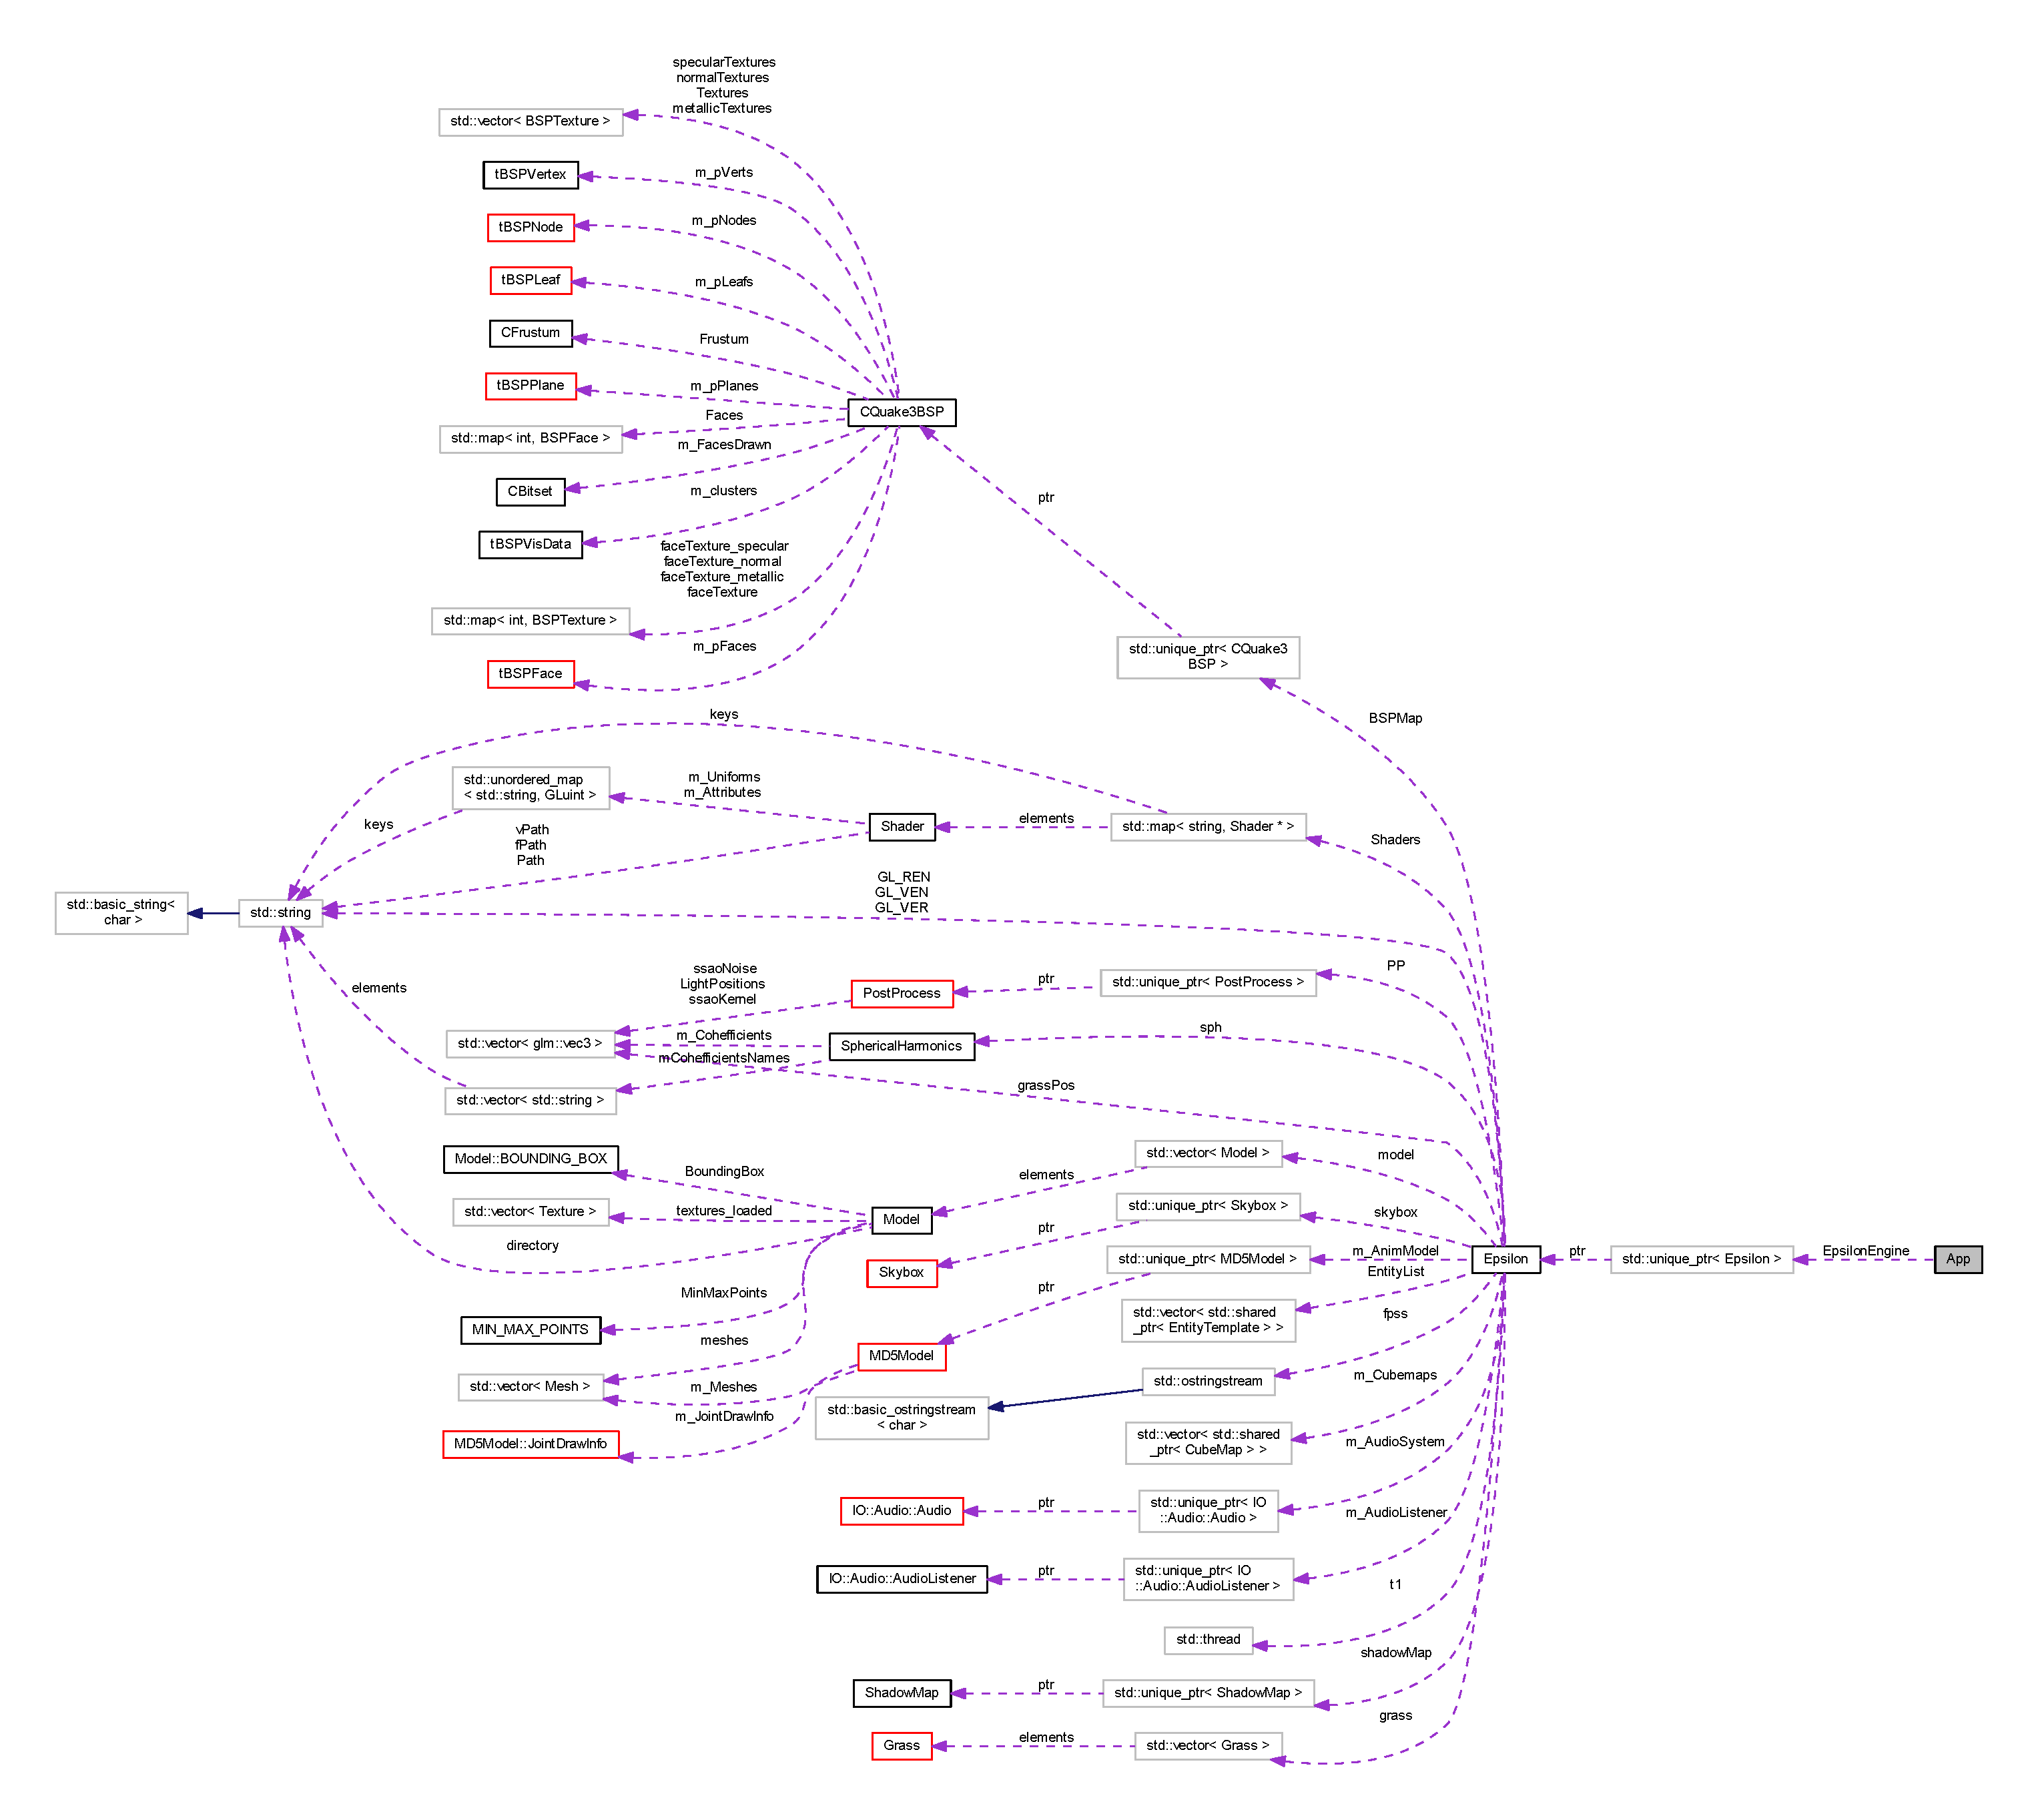
\includegraphics[width=350pt]{class_app__coll__graph}
\end{center}
\end{figure}
\subsection*{Public Member Functions}
\begin{DoxyCompactItemize}
\item 
{\bfseries App} (G\+L\+F\+Wwindow $\ast$\&win)\hypertarget{class_app_a4e1aff51a838dd4249f9a222cb01453e}{}\label{class_app_a4e1aff51a838dd4249f9a222cb01453e}

\item 
void {\bfseries Run} (void)\hypertarget{class_app_a48d0843a8f5eb7be1fd589df838d5b56}{}\label{class_app_a48d0843a8f5eb7be1fd589df838d5b56}

\end{DoxyCompactItemize}
\subsection*{Data Fields}
\begin{DoxyCompactItemize}
\item 
std\+::unique\+\_\+ptr$<$ \hyperlink{class_epsilon}{Epsilon} $>$ {\bfseries Epsilon\+Engine}\hypertarget{class_app_a13d267e75cc370f7a495d0140756f2ae}{}\label{class_app_a13d267e75cc370f7a495d0140756f2ae}

\end{DoxyCompactItemize}


\subsection{Detailed Description}
========= Copyright Survtech, All rights reserved. ============//

Purpose\+: 

 

Definition at line 13 of file main.\+h.


\hypertarget{class_i_o_1_1_audio_1_1_audio}{}\section{IO\+:\+:Audio\+:\+:Audio Class Reference}
\label{class_i_o_1_1_audio_1_1_audio}\index{I\+O\+::\+Audio\+::\+Audio@{I\+O\+::\+Audio\+::\+Audio}}


Collaboration diagram for IO\+:\+:Audio\+:\+:Audio\+:
\nopagebreak
\begin{figure}[H]
\begin{center}
\leavevmode
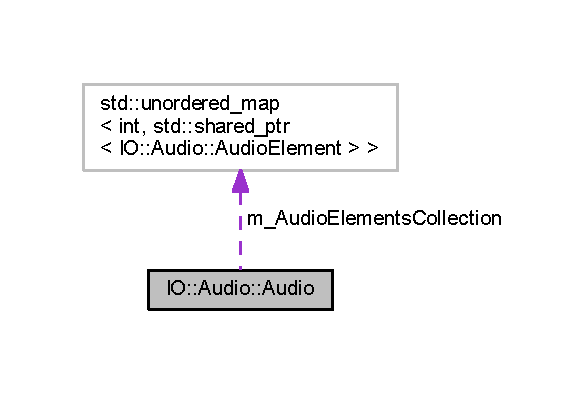
\includegraphics[width=282pt]{class_i_o_1_1_audio_1_1_audio__coll__graph}
\end{center}
\end{figure}
\subsection*{Public Member Functions}
\begin{DoxyCompactItemize}
\item 
void {\bfseries add\+Audio\+Element} (int, std\+::shared\+\_\+ptr$<$ \hyperlink{class_i_o_1_1_audio_1_1_audio_element}{Audio\+Element} $>$ element)\hypertarget{class_i_o_1_1_audio_1_1_audio_ab94ccbb6449e5c67b79af089ce675e3d}{}\label{class_i_o_1_1_audio_1_1_audio_ab94ccbb6449e5c67b79af089ce675e3d}

\item 
void {\bfseries Play\+Audio} ()\hypertarget{class_i_o_1_1_audio_1_1_audio_a47f7812040aef0d2f660cad5464d030a}{}\label{class_i_o_1_1_audio_1_1_audio_a47f7812040aef0d2f660cad5464d030a}

\item 
void {\bfseries Play\+By\+ID} (int)\hypertarget{class_i_o_1_1_audio_1_1_audio_aa7322292671539512a6d8eec3908a029}{}\label{class_i_o_1_1_audio_1_1_audio_aa7322292671539512a6d8eec3908a029}

\item 
bool {\bfseries set\+Master\+Volume} (float)\hypertarget{class_i_o_1_1_audio_1_1_audio_abc127574c67bd014fce4e4ec9f86002b}{}\label{class_i_o_1_1_audio_1_1_audio_abc127574c67bd014fce4e4ec9f86002b}

\item 
bool {\bfseries set\+Music\+Volume} (float)\hypertarget{class_i_o_1_1_audio_1_1_audio_a4bd5a3dfbcd8f5f6af8e067ecc535791}{}\label{class_i_o_1_1_audio_1_1_audio_a4bd5a3dfbcd8f5f6af8e067ecc535791}

\item 
bool {\bfseries set\+Game\+Volume} (float)\hypertarget{class_i_o_1_1_audio_1_1_audio_a57e02f1b176f94707ed7704b1d9e348a}{}\label{class_i_o_1_1_audio_1_1_audio_a57e02f1b176f94707ed7704b1d9e348a}

\end{DoxyCompactItemize}
\subsection*{Private Attributes}
\begin{DoxyCompactItemize}
\item 
float {\bfseries m\+\_\+\+Master\+Volume}\hypertarget{class_i_o_1_1_audio_1_1_audio_a9559f0dca415c5764d686062884ac1cf}{}\label{class_i_o_1_1_audio_1_1_audio_a9559f0dca415c5764d686062884ac1cf}

\item 
float {\bfseries m\+\_\+\+Music\+Volume}\hypertarget{class_i_o_1_1_audio_1_1_audio_a1f3534128042225669467fa0d1f839c2}{}\label{class_i_o_1_1_audio_1_1_audio_a1f3534128042225669467fa0d1f839c2}

\item 
float {\bfseries m\+\_\+\+Game\+Volume}\hypertarget{class_i_o_1_1_audio_1_1_audio_a3b8a67062fe14330aa1da8bc1b1001f9}{}\label{class_i_o_1_1_audio_1_1_audio_a3b8a67062fe14330aa1da8bc1b1001f9}

\item 
A\+L\+Cdevice $\ast$ {\bfseries device}\hypertarget{class_i_o_1_1_audio_1_1_audio_ac3e39acf964905bc2d113d846b0c8bc2}{}\label{class_i_o_1_1_audio_1_1_audio_ac3e39acf964905bc2d113d846b0c8bc2}

\item 
A\+L\+Ccontext $\ast$ {\bfseries context}\hypertarget{class_i_o_1_1_audio_1_1_audio_a87634f06b7f51d2404e427cc6102046f}{}\label{class_i_o_1_1_audio_1_1_audio_a87634f06b7f51d2404e427cc6102046f}

\item 
std\+::unordered\+\_\+map$<$ int, std\+::shared\+\_\+ptr$<$ \hyperlink{class_i_o_1_1_audio_1_1_audio_element}{Audio\+Element} $>$ $>$ {\bfseries m\+\_\+\+Audio\+Elements\+Collection}\hypertarget{class_i_o_1_1_audio_1_1_audio_afa7fe54debf2c73565314da2ca96081f}{}\label{class_i_o_1_1_audio_1_1_audio_afa7fe54debf2c73565314da2ca96081f}

\end{DoxyCompactItemize}


\subsection{Detailed Description}


Definition at line 9 of file Audio.\+h.


\hypertarget{class_i_o_1_1_audio_1_1_audio_element}{}\section{IO\+:\+:Audio\+:\+:Audio\+Element Class Reference}
\label{class_i_o_1_1_audio_1_1_audio_element}\index{I\+O\+::\+Audio\+::\+Audio\+Element@{I\+O\+::\+Audio\+::\+Audio\+Element}}
\subsection*{Public Member Functions}
\begin{DoxyCompactItemize}
\item 
{\bfseries Audio\+Element} (const char $\ast$file\+Name, A\+U\+D\+I\+O\+\_\+\+T\+Y\+PE type, glm\+::vec3 Audio\+Position, glm\+::vec3 Audio\+Direction)\hypertarget{class_i_o_1_1_audio_1_1_audio_element_a5dc9b2edcd68bbb0c17231628dead103}{}\label{class_i_o_1_1_audio_1_1_audio_element_a5dc9b2edcd68bbb0c17231628dead103}

\item 
void {\bfseries Destroy} ()\hypertarget{class_i_o_1_1_audio_1_1_audio_element_a0e9ba45fc7d2f2f3228695120ca0e539}{}\label{class_i_o_1_1_audio_1_1_audio_element_a0e9ba45fc7d2f2f3228695120ca0e539}

\item 
void {\bfseries Play} ()\hypertarget{class_i_o_1_1_audio_1_1_audio_element_ae6dd75379691f87959a93110bd456be7}{}\label{class_i_o_1_1_audio_1_1_audio_element_ae6dd75379691f87959a93110bd456be7}

\item 
A\+U\+D\+I\+O\+\_\+\+T\+Y\+PE {\bfseries get\+Type} ()\hypertarget{class_i_o_1_1_audio_1_1_audio_element_aaa1929ed8868b03997adebca0a9f2fa7}{}\label{class_i_o_1_1_audio_1_1_audio_element_aaa1929ed8868b03997adebca0a9f2fa7}

\end{DoxyCompactItemize}
\subsection*{Private Attributes}
\begin{DoxyCompactItemize}
\item 
unsigned int {\bfseries m\+\_\+\+Audio\+ID}\hypertarget{class_i_o_1_1_audio_1_1_audio_element_a527eaf6c623d65e34f858c8e9445fa5e}{}\label{class_i_o_1_1_audio_1_1_audio_element_a527eaf6c623d65e34f858c8e9445fa5e}

\item 
unsigned int {\bfseries m\+\_\+\+Buffer\+ID}\hypertarget{class_i_o_1_1_audio_1_1_audio_element_a3ec6a87075a8df60de7c632ce554474a}{}\label{class_i_o_1_1_audio_1_1_audio_element_a3ec6a87075a8df60de7c632ce554474a}

\item 
float {\bfseries m\+\_\+\+Volume}\hypertarget{class_i_o_1_1_audio_1_1_audio_element_a9a370abcfaea4f25da82691fdc02289d}{}\label{class_i_o_1_1_audio_1_1_audio_element_a9a370abcfaea4f25da82691fdc02289d}

\item 
int {\bfseries m\+\_\+\+Channels}\hypertarget{class_i_o_1_1_audio_1_1_audio_element_a0a4ba6e76a29da2a3d7587c574ed7cba}{}\label{class_i_o_1_1_audio_1_1_audio_element_a0a4ba6e76a29da2a3d7587c574ed7cba}

\item 
unsigned int {\bfseries m\+\_\+\+Format}\hypertarget{class_i_o_1_1_audio_1_1_audio_element_ab31b6315ede0f2c568dffe14eb02ae32}{}\label{class_i_o_1_1_audio_1_1_audio_element_ab31b6315ede0f2c568dffe14eb02ae32}

\item 
int {\bfseries m\+\_\+\+Bytes\+Per\+Second}\hypertarget{class_i_o_1_1_audio_1_1_audio_element_af2b400f9761b0b33a81bb65f25532866}{}\label{class_i_o_1_1_audio_1_1_audio_element_af2b400f9761b0b33a81bb65f25532866}

\item 
std\+::shared\+\_\+ptr$<$ char $>$ {\bfseries data}\hypertarget{class_i_o_1_1_audio_1_1_audio_element_a5a89ff073db45b715cc9f0162e71354f}{}\label{class_i_o_1_1_audio_1_1_audio_element_a5a89ff073db45b715cc9f0162e71354f}

\item 
A\+U\+D\+I\+O\+\_\+\+T\+Y\+PE {\bfseries m\+\_\+\+Type}\hypertarget{class_i_o_1_1_audio_1_1_audio_element_a867da6202123d156f61dc57bcc5fc645}{}\label{class_i_o_1_1_audio_1_1_audio_element_a867da6202123d156f61dc57bcc5fc645}

\item 
glm\+::vec3 {\bfseries m\+\_\+\+Position}\hypertarget{class_i_o_1_1_audio_1_1_audio_element_aeac2de4d6e56351d66072ff105c92069}{}\label{class_i_o_1_1_audio_1_1_audio_element_aeac2de4d6e56351d66072ff105c92069}

\item 
glm\+::vec3 {\bfseries m\+\_\+\+Direction}\hypertarget{class_i_o_1_1_audio_1_1_audio_element_a8186dfc5446ca0409f7c259eb2a9f222}{}\label{class_i_o_1_1_audio_1_1_audio_element_a8186dfc5446ca0409f7c259eb2a9f222}

\item 
glm\+::vec3 {\bfseries m\+\_\+\+Velocity}\hypertarget{class_i_o_1_1_audio_1_1_audio_element_a0b68136368101c51108886435dd94b00}{}\label{class_i_o_1_1_audio_1_1_audio_element_a0b68136368101c51108886435dd94b00}

\item 
float {\bfseries m\+\_\+\+Radius}\hypertarget{class_i_o_1_1_audio_1_1_audio_element_a08db2f7eadcda0d391722723afb68bca}{}\label{class_i_o_1_1_audio_1_1_audio_element_a08db2f7eadcda0d391722723afb68bca}

\end{DoxyCompactItemize}


\subsection{Detailed Description}


Definition at line 10 of file Audio\+Element.\+h.


\hypertarget{class_i_o_1_1_audio_1_1_audio_listener}{}\section{IO\+:\+:Audio\+:\+:Audio\+Listener Class Reference}
\label{class_i_o_1_1_audio_1_1_audio_listener}\index{I\+O\+::\+Audio\+::\+Audio\+Listener@{I\+O\+::\+Audio\+::\+Audio\+Listener}}
\subsection*{Public Member Functions}
\begin{DoxyCompactItemize}
\item 
void {\bfseries Update\+Listener} ()\hypertarget{class_i_o_1_1_audio_1_1_audio_listener_a8ecb93a04ab93ae63d6c23e5a6035364}{}\label{class_i_o_1_1_audio_1_1_audio_listener_a8ecb93a04ab93ae63d6c23e5a6035364}

\item 
void {\bfseries set\+Listener\+Position} (glm\+::vec3 pos)\hypertarget{class_i_o_1_1_audio_1_1_audio_listener_a3eeb956aea0c66124ee265b04d5b6c14}{}\label{class_i_o_1_1_audio_1_1_audio_listener_a3eeb956aea0c66124ee265b04d5b6c14}

\item 
void {\bfseries set\+Listener\+Direction} (glm\+::vec3 dir)\hypertarget{class_i_o_1_1_audio_1_1_audio_listener_afd39011a9bd287b6288c1f08db25282b}{}\label{class_i_o_1_1_audio_1_1_audio_listener_afd39011a9bd287b6288c1f08db25282b}

\item 
glm\+::vec3 {\bfseries get\+Listener\+Position} () const \hypertarget{class_i_o_1_1_audio_1_1_audio_listener_aa06927e5688b7473bb85874e048b036f}{}\label{class_i_o_1_1_audio_1_1_audio_listener_aa06927e5688b7473bb85874e048b036f}

\item 
glm\+::vec3 {\bfseries get\+Listener\+Direction} () const \hypertarget{class_i_o_1_1_audio_1_1_audio_listener_ab6782fcfaa5c14aedf9222dc58e73c83}{}\label{class_i_o_1_1_audio_1_1_audio_listener_ab6782fcfaa5c14aedf9222dc58e73c83}

\end{DoxyCompactItemize}
\subsection*{Private Attributes}
\begin{DoxyCompactItemize}
\item 
glm\+::vec3 {\bfseries m\+\_\+\+Listener\+Position}\hypertarget{class_i_o_1_1_audio_1_1_audio_listener_a8423bc9e78d1cb76c7262630d0a66b73}{}\label{class_i_o_1_1_audio_1_1_audio_listener_a8423bc9e78d1cb76c7262630d0a66b73}

\item 
glm\+::vec3 {\bfseries m\+\_\+\+Listener\+Direction}\hypertarget{class_i_o_1_1_audio_1_1_audio_listener_a4b2875262a1f507955ce0b234a00aaf6}{}\label{class_i_o_1_1_audio_1_1_audio_listener_a4b2875262a1f507955ce0b234a00aaf6}

\item 
float {\bfseries m\+\_\+\+Listener\+Orientation} \mbox{[}6\mbox{]}\hypertarget{class_i_o_1_1_audio_1_1_audio_listener_a4bf95f2c7169fd0df97e064e35b972ce}{}\label{class_i_o_1_1_audio_1_1_audio_listener_a4bf95f2c7169fd0df97e064e35b972ce}

\item 
float {\bfseries m\+\_\+\+Listener\+Velocity}\hypertarget{class_i_o_1_1_audio_1_1_audio_listener_a66bba80d99062e6451e859ec8b22af43}{}\label{class_i_o_1_1_audio_1_1_audio_listener_a66bba80d99062e6451e859ec8b22af43}

\end{DoxyCompactItemize}


\subsection{Detailed Description}


Definition at line 9 of file Audio\+Listener.\+h.


\hypertarget{struct_m_d5_animation_1_1_base_frame}{}\section{M\+D5\+Animation\+:\+:Base\+Frame Struct Reference}
\label{struct_m_d5_animation_1_1_base_frame}\index{M\+D5\+Animation\+::\+Base\+Frame@{M\+D5\+Animation\+::\+Base\+Frame}}
\subsection*{Data Fields}
\begin{DoxyCompactItemize}
\item 
glm\+::vec3 {\bfseries m\+\_\+\+Pos}\hypertarget{struct_m_d5_animation_1_1_base_frame_a9586b0574582517cc2968703e07588b0}{}\label{struct_m_d5_animation_1_1_base_frame_a9586b0574582517cc2968703e07588b0}

\item 
glm\+::quat {\bfseries m\+\_\+\+Orient}\hypertarget{struct_m_d5_animation_1_1_base_frame_ae60903c1a92bf95597fa9c5c963d0ea9}{}\label{struct_m_d5_animation_1_1_base_frame_ae60903c1a92bf95597fa9c5c963d0ea9}

\end{DoxyCompactItemize}


\subsection{Detailed Description}


Definition at line 41 of file M\+D5\+\_\+\+Anim.\+h.


\hypertarget{struct_b_i_t_m_a_p___i_n_f_o_r_m_a_t_i_o_n___h_e_a_d_e_r}{}\section{B\+I\+T\+M\+A\+P\+\_\+\+I\+N\+F\+O\+R\+M\+A\+T\+I\+O\+N\+\_\+\+H\+E\+A\+D\+ER Struct Reference}
\label{struct_b_i_t_m_a_p___i_n_f_o_r_m_a_t_i_o_n___h_e_a_d_e_r}\index{B\+I\+T\+M\+A\+P\+\_\+\+I\+N\+F\+O\+R\+M\+A\+T\+I\+O\+N\+\_\+\+H\+E\+A\+D\+ER@{B\+I\+T\+M\+A\+P\+\_\+\+I\+N\+F\+O\+R\+M\+A\+T\+I\+O\+N\+\_\+\+H\+E\+A\+D\+ER}}
\subsection*{Data Fields}
\begin{DoxyCompactItemize}
\item 
I\+NT {\bfseries B\+I\+T\+M\+A\+P\+I\+N\+F\+O\+H\+E\+A\+D\+E\+R\+\_\+\+S\+I\+ZE}\hypertarget{struct_b_i_t_m_a_p___i_n_f_o_r_m_a_t_i_o_n___h_e_a_d_e_r_afd4ca64510fe69034359f6065ad1d34f}{}\label{struct_b_i_t_m_a_p___i_n_f_o_r_m_a_t_i_o_n___h_e_a_d_e_r_afd4ca64510fe69034359f6065ad1d34f}

\item 
I\+NT {\bfseries W\+I\+D\+TH}\hypertarget{struct_b_i_t_m_a_p___i_n_f_o_r_m_a_t_i_o_n___h_e_a_d_e_r_a03be4a250788c557d73dd54ee79093d9}{}\label{struct_b_i_t_m_a_p___i_n_f_o_r_m_a_t_i_o_n___h_e_a_d_e_r_a03be4a250788c557d73dd54ee79093d9}

\item 
I\+NT {\bfseries H\+E\+I\+G\+HT}\hypertarget{struct_b_i_t_m_a_p___i_n_f_o_r_m_a_t_i_o_n___h_e_a_d_e_r_a6c8f69ac4a9418a6d7e53b4d3c302aa8}{}\label{struct_b_i_t_m_a_p___i_n_f_o_r_m_a_t_i_o_n___h_e_a_d_e_r_a6c8f69ac4a9418a6d7e53b4d3c302aa8}

\item 
S\+H\+O\+RT {\bfseries N\+U\+M\+\_\+\+P\+L\+A\+N\+ES}\hypertarget{struct_b_i_t_m_a_p___i_n_f_o_r_m_a_t_i_o_n___h_e_a_d_e_r_a0f9264746215b896b69bd8ac29981c2a}{}\label{struct_b_i_t_m_a_p___i_n_f_o_r_m_a_t_i_o_n___h_e_a_d_e_r_a0f9264746215b896b69bd8ac29981c2a}

\item 
S\+H\+O\+RT {\bfseries B\+PP}\hypertarget{struct_b_i_t_m_a_p___i_n_f_o_r_m_a_t_i_o_n___h_e_a_d_e_r_a78dabb55fff1abfb2e97a7bc2de17610}{}\label{struct_b_i_t_m_a_p___i_n_f_o_r_m_a_t_i_o_n___h_e_a_d_e_r_a78dabb55fff1abfb2e97a7bc2de17610}

\item 
I\+NT {\bfseries C\+O\+M\+P\+R\+E\+S\+S\+I\+ON}\hypertarget{struct_b_i_t_m_a_p___i_n_f_o_r_m_a_t_i_o_n___h_e_a_d_e_r_a7727be08d81df600cfbd75c458ef2169}{}\label{struct_b_i_t_m_a_p___i_n_f_o_r_m_a_t_i_o_n___h_e_a_d_e_r_a7727be08d81df600cfbd75c458ef2169}

\item 
I\+NT {\bfseries S\+I\+ZE}\hypertarget{struct_b_i_t_m_a_p___i_n_f_o_r_m_a_t_i_o_n___h_e_a_d_e_r_a6d728081de4ad2b38a7a9bf723f3078c}{}\label{struct_b_i_t_m_a_p___i_n_f_o_r_m_a_t_i_o_n___h_e_a_d_e_r_a6d728081de4ad2b38a7a9bf723f3078c}

\item 
I\+NT {\bfseries H\+O\+R\+I\+Z\+O\+N\+T\+A\+L\+\_\+\+R\+E\+S\+O\+L\+U\+T\+I\+ON}\hypertarget{struct_b_i_t_m_a_p___i_n_f_o_r_m_a_t_i_o_n___h_e_a_d_e_r_a1ea6aa22d546339fa03731bd56d7bb1b}{}\label{struct_b_i_t_m_a_p___i_n_f_o_r_m_a_t_i_o_n___h_e_a_d_e_r_a1ea6aa22d546339fa03731bd56d7bb1b}

\item 
I\+NT {\bfseries V\+E\+R\+T\+I\+C\+A\+L\+\_\+\+R\+E\+S\+O\+L\+U\+T\+I\+ON}\hypertarget{struct_b_i_t_m_a_p___i_n_f_o_r_m_a_t_i_o_n___h_e_a_d_e_r_a50812bcda652fe8377b85b1e9779d507}{}\label{struct_b_i_t_m_a_p___i_n_f_o_r_m_a_t_i_o_n___h_e_a_d_e_r_a50812bcda652fe8377b85b1e9779d507}

\item 
I\+NT {\bfseries N\+U\+M\+\_\+\+C\+O\+L\+O\+RS}\hypertarget{struct_b_i_t_m_a_p___i_n_f_o_r_m_a_t_i_o_n___h_e_a_d_e_r_a3badf5ea06bb1d9e0d423a6fd35d2357}{}\label{struct_b_i_t_m_a_p___i_n_f_o_r_m_a_t_i_o_n___h_e_a_d_e_r_a3badf5ea06bb1d9e0d423a6fd35d2357}

\item 
I\+NT {\bfseries N\+U\+M\+\_\+\+I\+M\+P\+O\+R\+T\+A\+N\+T\+\_\+\+C\+O\+L\+O\+RS}\hypertarget{struct_b_i_t_m_a_p___i_n_f_o_r_m_a_t_i_o_n___h_e_a_d_e_r_aa1cd6991598b67ada844d78b697337d5}{}\label{struct_b_i_t_m_a_p___i_n_f_o_r_m_a_t_i_o_n___h_e_a_d_e_r_aa1cd6991598b67ada844d78b697337d5}

\end{DoxyCompactItemize}


\subsection{Detailed Description}


Definition at line 23 of file B\+M\+P.\+hpp.


\hypertarget{struct_b_m_p___h_e_a_d_e_r}{}\section{B\+M\+P\+\_\+\+H\+E\+A\+D\+ER Struct Reference}
\label{struct_b_m_p___h_e_a_d_e_r}\index{B\+M\+P\+\_\+\+H\+E\+A\+D\+ER@{B\+M\+P\+\_\+\+H\+E\+A\+D\+ER}}
\subsection*{Data Fields}
\begin{DoxyCompactItemize}
\item 
S\+H\+O\+RT {\bfseries \+\_\+signature}\hypertarget{struct_b_m_p___h_e_a_d_e_r_a8e28f3e072eda68a6f360fe280a63d66}{}\label{struct_b_m_p___h_e_a_d_e_r_a8e28f3e072eda68a6f360fe280a63d66}

\item 
I\+NT {\bfseries \+\_\+size}\hypertarget{struct_b_m_p___h_e_a_d_e_r_aec195a5228186b9c32f8a93133b5a9b9}{}\label{struct_b_m_p___h_e_a_d_e_r_aec195a5228186b9c32f8a93133b5a9b9}

\item 
S\+H\+O\+RT {\bfseries \+\_\+reserved}\hypertarget{struct_b_m_p___h_e_a_d_e_r_ad64eddcac86911e65d41955b0b15744e}{}\label{struct_b_m_p___h_e_a_d_e_r_ad64eddcac86911e65d41955b0b15744e}

\item 
S\+H\+O\+RT {\bfseries \+\_\+\+\_\+reserved}\hypertarget{struct_b_m_p___h_e_a_d_e_r_a299e66558c91abdabe3a661c257329f9}{}\label{struct_b_m_p___h_e_a_d_e_r_a299e66558c91abdabe3a661c257329f9}

\item 
I\+NT {\bfseries \+\_\+offset}\hypertarget{struct_b_m_p___h_e_a_d_e_r_a0ae360efd03820bad6781c1ecb6073e9}{}\label{struct_b_m_p___h_e_a_d_e_r_a0ae360efd03820bad6781c1ecb6073e9}

\end{DoxyCompactItemize}


\subsection{Detailed Description}


Definition at line 14 of file B\+M\+P.\+hpp.


\hypertarget{struct_m_d5_animation_1_1_bound}{}\section{M\+D5\+Animation\+:\+:Bound Struct Reference}
\label{struct_m_d5_animation_1_1_bound}\index{M\+D5\+Animation\+::\+Bound@{M\+D5\+Animation\+::\+Bound}}
\subsection*{Data Fields}
\begin{DoxyCompactItemize}
\item 
glm\+::vec3 {\bfseries m\+\_\+\+Min}\hypertarget{struct_m_d5_animation_1_1_bound_ac336feaf8013f6da93cd776c0e2ebd16}{}\label{struct_m_d5_animation_1_1_bound_ac336feaf8013f6da93cd776c0e2ebd16}

\item 
glm\+::vec3 {\bfseries m\+\_\+\+Max}\hypertarget{struct_m_d5_animation_1_1_bound_a9beb9b46e65c5314646761b4a0fec54e}{}\label{struct_m_d5_animation_1_1_bound_a9beb9b46e65c5314646761b4a0fec54e}

\end{DoxyCompactItemize}


\subsection{Detailed Description}


Definition at line 34 of file M\+D5\+\_\+\+Anim.\+h.


\hypertarget{struct_model_1_1_b_o_u_n_d_i_n_g___b_o_x}{}\section{Model\+:\+:B\+O\+U\+N\+D\+I\+N\+G\+\_\+\+B\+OX Struct Reference}
\label{struct_model_1_1_b_o_u_n_d_i_n_g___b_o_x}\index{Model\+::\+B\+O\+U\+N\+D\+I\+N\+G\+\_\+\+B\+OX@{Model\+::\+B\+O\+U\+N\+D\+I\+N\+G\+\_\+\+B\+OX}}


Structure to store the models bounding box for visibility and collision computation.  


\subsection*{Data Fields}
\begin{DoxyCompactItemize}
\item 
float {\bfseries F\+R\+O\+N\+T\+\_\+\+T\+O\+P\+\_\+\+L\+E\+FT}\hypertarget{struct_model_1_1_b_o_u_n_d_i_n_g___b_o_x_a65787e6454e3e94e8144a039fe5eb1fc}{}\label{struct_model_1_1_b_o_u_n_d_i_n_g___b_o_x_a65787e6454e3e94e8144a039fe5eb1fc}

\item 
float {\bfseries F\+R\+O\+N\+T\+\_\+\+T\+O\+P\+\_\+\+R\+I\+G\+HT}\hypertarget{struct_model_1_1_b_o_u_n_d_i_n_g___b_o_x_a9ed20b67bb450f2e9dcb2f81265faaba}{}\label{struct_model_1_1_b_o_u_n_d_i_n_g___b_o_x_a9ed20b67bb450f2e9dcb2f81265faaba}

\item 
float {\bfseries F\+R\+O\+N\+T\+\_\+\+B\+O\+T\+T\+O\+M\+\_\+\+L\+E\+FT}\hypertarget{struct_model_1_1_b_o_u_n_d_i_n_g___b_o_x_afd1d232efb0ca43160624cf3ae2b0ae6}{}\label{struct_model_1_1_b_o_u_n_d_i_n_g___b_o_x_afd1d232efb0ca43160624cf3ae2b0ae6}

\item 
float {\bfseries F\+R\+O\+N\+T\+\_\+\+B\+O\+T\+T\+O\+M\+\_\+\+R\+I\+G\+HT}\hypertarget{struct_model_1_1_b_o_u_n_d_i_n_g___b_o_x_a8cbb072a587d3453f961c0bb3cae0e59}{}\label{struct_model_1_1_b_o_u_n_d_i_n_g___b_o_x_a8cbb072a587d3453f961c0bb3cae0e59}

\item 
float {\bfseries B\+A\+C\+K\+\_\+\+T\+O\+P\+\_\+\+L\+E\+FT}\hypertarget{struct_model_1_1_b_o_u_n_d_i_n_g___b_o_x_aeb402ac7832ab6f1af573d85e64fe8a2}{}\label{struct_model_1_1_b_o_u_n_d_i_n_g___b_o_x_aeb402ac7832ab6f1af573d85e64fe8a2}

\item 
float {\bfseries B\+A\+C\+K\+\_\+\+T\+O\+P\+\_\+\+R\+I\+G\+HT}\hypertarget{struct_model_1_1_b_o_u_n_d_i_n_g___b_o_x_a43ea2d971ded0474794af07faa97bf68}{}\label{struct_model_1_1_b_o_u_n_d_i_n_g___b_o_x_a43ea2d971ded0474794af07faa97bf68}

\item 
float {\bfseries B\+A\+C\+K\+\_\+\+B\+O\+T\+T\+O\+M\+\_\+\+L\+E\+FT}\hypertarget{struct_model_1_1_b_o_u_n_d_i_n_g___b_o_x_af4c6ec7fac905c1ff6c2eeccc8272b7f}{}\label{struct_model_1_1_b_o_u_n_d_i_n_g___b_o_x_af4c6ec7fac905c1ff6c2eeccc8272b7f}

\item 
float {\bfseries B\+A\+C\+K\+\_\+\+B\+O\+T\+T\+O\+M\+\_\+\+R\+I\+G\+HT}\hypertarget{struct_model_1_1_b_o_u_n_d_i_n_g___b_o_x_af638a06a328c69636b4e261a10940d1e}{}\label{struct_model_1_1_b_o_u_n_d_i_n_g___b_o_x_af638a06a328c69636b4e261a10940d1e}

\end{DoxyCompactItemize}


\subsection{Detailed Description}
Structure to store the models bounding box for visibility and collision computation. 

Definition at line 102 of file Model.\+h.


\hypertarget{class_b_s_p_face}{}\section{B\+S\+P\+Face Class Reference}
\label{class_b_s_p_face}\index{B\+S\+P\+Face@{B\+S\+P\+Face}}


Collaboration diagram for B\+S\+P\+Face\+:
\nopagebreak
\begin{figure}[H]
\begin{center}
\leavevmode
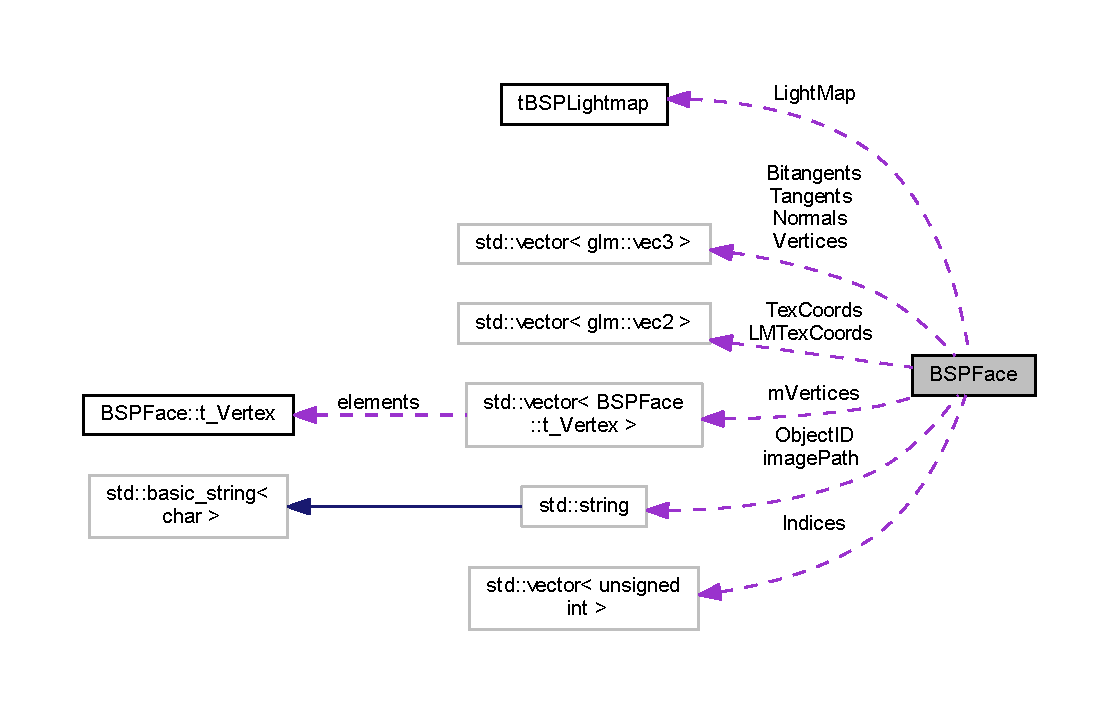
\includegraphics[width=350pt]{class_b_s_p_face__coll__graph}
\end{center}
\end{figure}
\subsection*{Data Structures}
\begin{DoxyCompactItemize}
\item 
struct \hyperlink{struct_b_s_p_face_1_1t___vertex}{t\+\_\+\+Vertex}
\end{DoxyCompactItemize}
\subsection*{Public Member Functions}
\begin{DoxyCompactItemize}
\item 
bool \hyperlink{class_b_s_p_face_a4ae99df1fc45845b5a3049c73eb6ae25}{Build\+Face} (std\+::vector$<$ glm\+::vec3 $>$ Vertices, std\+::vector$<$ glm\+::vec3 $>$ Normals, std\+::vector$<$ glm\+::vec2 $>$ Tex\+Coords, std\+::vector$<$ glm\+::vec2 $>$ L\+M\+Tex\+Coords, std\+::vector$<$ unsigned int $>$ Indices, int ID, string image\+Path, \hyperlink{structt_b_s_p_lightmap}{t\+B\+S\+P\+Lightmap} Light\+Map, std\+::shared\+\_\+ptr$<$ \hyperlink{class_resource_manager}{Resource\+Manager} $>$ Resm)
\item 
void {\bfseries Render\+Face} (G\+Luint shader, G\+Luint Texture\+ID, G\+Luint normal\+ID, G\+Luint specular\+ID, G\+Luint metallic\+ID, bool)\hypertarget{class_b_s_p_face_a254a767339d20aef7b14ab5c0d57406d}{}\label{class_b_s_p_face_a254a767339d20aef7b14ab5c0d57406d}

\item 
std\+::string {\bfseries get\+Object\+ID} ()\hypertarget{class_b_s_p_face_a4ca1b71cb722d7bb4f22b04ff5c3a9a3}{}\label{class_b_s_p_face_a4ca1b71cb722d7bb4f22b04ff5c3a9a3}

\end{DoxyCompactItemize}
\subsection*{Data Fields}
\begin{DoxyCompactItemize}
\item 
std\+::string {\bfseries Object\+ID}\hypertarget{class_b_s_p_face_a7c79a08c838144cdd0146172b6c4f6c1}{}\label{class_b_s_p_face_a7c79a08c838144cdd0146172b6c4f6c1}

\item 
int {\bfseries face\+ID}\hypertarget{class_b_s_p_face_a2f3839071b0408b173a00aa98b987e4e}{}\label{class_b_s_p_face_a2f3839071b0408b173a00aa98b987e4e}

\item 
std\+::shared\+\_\+ptr$<$ bt\+Rigid\+Body $>$ {\bfseries rigid\+Body}\hypertarget{class_b_s_p_face_af74bd1f8ab6d7510ef500bcbcc9597fb}{}\label{class_b_s_p_face_af74bd1f8ab6d7510ef500bcbcc9597fb}

\end{DoxyCompactItemize}
\subsection*{Private Member Functions}
\begin{DoxyCompactItemize}
\item 
bool {\bfseries Load\+Light\+Map\+Texture} ()\hypertarget{class_b_s_p_face_aff2c541edb2cfb6826ac8a1af5d34020}{}\label{class_b_s_p_face_aff2c541edb2cfb6826ac8a1af5d34020}

\item 
bool \hyperlink{class_b_s_p_face_a5814b00d0169b2eb7808c0d64724dd94}{Calc\+Tangent\+Space} ()
\item 
bool \hyperlink{class_b_s_p_face_a53ccd893ab6d659edb33fb09de00d7be}{prepare\+V\+AO} ()
\end{DoxyCompactItemize}
\subsection*{Private Attributes}
\begin{DoxyCompactItemize}
\item 
std\+::vector$<$ \hyperlink{struct_b_s_p_face_1_1t___vertex}{t\+\_\+\+Vertex} $>$ {\bfseries m\+Vertices}\hypertarget{class_b_s_p_face_ad5ebb6100ab23467e7737c25fd8e8523}{}\label{class_b_s_p_face_ad5ebb6100ab23467e7737c25fd8e8523}

\item 
glm\+::vec3 {\bfseries m\+Position}\hypertarget{class_b_s_p_face_a99cf0e5077e2ec7386b2d7ca18dbaf69}{}\label{class_b_s_p_face_a99cf0e5077e2ec7386b2d7ca18dbaf69}

\item 
G\+Luint {\bfseries V\+AO}\hypertarget{class_b_s_p_face_a37f5fb2c6dc1fca509a3270de9d63d5f}{}\label{class_b_s_p_face_a37f5fb2c6dc1fca509a3270de9d63d5f}

\item 
G\+Luint {\bfseries texture}\hypertarget{class_b_s_p_face_a70b3c4166cf280c5c2ff0268b7acafbf}{}\label{class_b_s_p_face_a70b3c4166cf280c5c2ff0268b7acafbf}

\item 
string {\bfseries image\+Path}\hypertarget{class_b_s_p_face_a0ba38134841b9f59d1f430aef37a87ca}{}\label{class_b_s_p_face_a0ba38134841b9f59d1f430aef37a87ca}

\item 
G\+Luint {\bfseries V\+BO}\hypertarget{class_b_s_p_face_af68418b4c1d2714a2d1c2d07e90484d7}{}\label{class_b_s_p_face_af68418b4c1d2714a2d1c2d07e90484d7}

\item 
G\+Luint {\bfseries E\+BO}\hypertarget{class_b_s_p_face_aff1f36c5b368c9dad1b005083d087991}{}\label{class_b_s_p_face_aff1f36c5b368c9dad1b005083d087991}

\item 
G\+Luint {\bfseries G\+I\+Texture}\hypertarget{class_b_s_p_face_a9d8138d21cf83781f8feaacfc6744058}{}\label{class_b_s_p_face_a9d8138d21cf83781f8feaacfc6744058}

\item 
bool {\bfseries G\+I\+Set} = false\hypertarget{class_b_s_p_face_a7d14051390a327bc3476c2a68177cd5a}{}\label{class_b_s_p_face_a7d14051390a327bc3476c2a68177cd5a}

\item 
\hyperlink{structt_b_s_p_lightmap}{t\+B\+S\+P\+Lightmap} {\bfseries Light\+Map}\hypertarget{class_b_s_p_face_aea4a6c2edb342e354ef6290d2b27f5d7}{}\label{class_b_s_p_face_aea4a6c2edb342e354ef6290d2b27f5d7}

\item 
G\+Luint {\bfseries Light\+Maptexture}\hypertarget{class_b_s_p_face_aba7ea1972d5bd877c6e7221d2d44a518}{}\label{class_b_s_p_face_aba7ea1972d5bd877c6e7221d2d44a518}

\item 
std\+::shared\+\_\+ptr$<$ \hyperlink{class_physics_1_1_physic_object}{Physics\+::\+Physic\+Object} $>$ {\bfseries Collision\+Object}\hypertarget{class_b_s_p_face_a3911b146eb7a30813599dd9ef28147e1}{}\label{class_b_s_p_face_a3911b146eb7a30813599dd9ef28147e1}

\item 
std\+::shared\+\_\+ptr$<$ \hyperlink{class_resource_manager}{Resource\+Manager} $>$ {\bfseries resm}\hypertarget{class_b_s_p_face_a1b8547089bd3fa796772777b426fe916}{}\label{class_b_s_p_face_a1b8547089bd3fa796772777b426fe916}

\item 
std\+::vector$<$ glm\+::vec3 $>$ {\bfseries Vertices}\hypertarget{class_b_s_p_face_af5c2081505af9ca68f2fd11411accc61}{}\label{class_b_s_p_face_af5c2081505af9ca68f2fd11411accc61}

\item 
std\+::vector$<$ glm\+::vec3 $>$ {\bfseries Normals}\hypertarget{class_b_s_p_face_a007702ba00244c56eaddd574c1101f94}{}\label{class_b_s_p_face_a007702ba00244c56eaddd574c1101f94}

\item 
std\+::vector$<$ glm\+::vec2 $>$ {\bfseries Tex\+Coords}\hypertarget{class_b_s_p_face_a732af8bbae1f7d05d6f208c5483b2097}{}\label{class_b_s_p_face_a732af8bbae1f7d05d6f208c5483b2097}

\item 
std\+::vector$<$ glm\+::vec2 $>$ {\bfseries L\+M\+Tex\+Coords}\hypertarget{class_b_s_p_face_acd850892f1a001b8c323648508c0357d}{}\label{class_b_s_p_face_acd850892f1a001b8c323648508c0357d}

\item 
std\+::vector$<$ glm\+::vec3 $>$ {\bfseries Tangents}\hypertarget{class_b_s_p_face_a7914de0eca3b3a656f2e5af1f989f270}{}\label{class_b_s_p_face_a7914de0eca3b3a656f2e5af1f989f270}

\item 
std\+::vector$<$ glm\+::vec3 $>$ {\bfseries Bitangents}\hypertarget{class_b_s_p_face_addc72ce0baed9dc6e61c802271de9503}{}\label{class_b_s_p_face_addc72ce0baed9dc6e61c802271de9503}

\item 
std\+::vector$<$ unsigned int $>$ {\bfseries Indices}\hypertarget{class_b_s_p_face_a5d53336515838573d7d619622664e51a}{}\label{class_b_s_p_face_a5d53336515838573d7d619622664e51a}

\item 
std\+::shared\+\_\+ptr$<$ \hyperlink{class_physics_1_1_collision_info}{Physics\+::\+Collision\+Info} $>$ {\bfseries collinfo}\hypertarget{class_b_s_p_face_acf76591e8fdb71bb1390a0685652ead9}{}\label{class_b_s_p_face_acf76591e8fdb71bb1390a0685652ead9}

\end{DoxyCompactItemize}


\subsection{Detailed Description}


Definition at line 30 of file B\+S\+P\+Face.\+h.



\subsection{Member Function Documentation}
\index{B\+S\+P\+Face@{B\+S\+P\+Face}!Build\+Face@{Build\+Face}}
\index{Build\+Face@{Build\+Face}!B\+S\+P\+Face@{B\+S\+P\+Face}}
\subsubsection[{\texorpdfstring{Build\+Face(std\+::vector$<$ glm\+::vec3 $>$ Vertices, std\+::vector$<$ glm\+::vec3 $>$ Normals, std\+::vector$<$ glm\+::vec2 $>$ Tex\+Coords, std\+::vector$<$ glm\+::vec2 $>$ L\+M\+Tex\+Coords, std\+::vector$<$ unsigned int $>$ Indices, int I\+D, string image\+Path, t\+B\+S\+P\+Lightmap Light\+Map, std\+::shared\+\_\+ptr$<$ Resource\+Manager $>$ Resm)}{BuildFace(std::vector< glm::vec3 > Vertices, std::vector< glm::vec3 > Normals, std::vector< glm::vec2 > TexCoords, std::vector< glm::vec2 > LMTexCoords, std::vector< unsigned int > Indices, int ID, string imagePath, tBSPLightmap LightMap, std::shared_ptr< ResourceManager > Resm)}}]{\setlength{\rightskip}{0pt plus 5cm}bool B\+S\+P\+Face\+::\+Build\+Face (
\begin{DoxyParamCaption}
\item[{std\+::vector$<$ glm\+::vec3 $>$}]{Vertices, }
\item[{std\+::vector$<$ glm\+::vec3 $>$}]{Normals, }
\item[{std\+::vector$<$ glm\+::vec2 $>$}]{Tex\+Coords, }
\item[{std\+::vector$<$ glm\+::vec2 $>$}]{L\+M\+Tex\+Coords, }
\item[{std\+::vector$<$ unsigned int $>$}]{Indices, }
\item[{int}]{ID, }
\item[{string}]{image\+Path, }
\item[{{\bf t\+B\+S\+P\+Lightmap}}]{Light\+Map, }
\item[{std\+::shared\+\_\+ptr$<$ {\bf Resource\+Manager} $>$}]{Resm}
\end{DoxyParamCaption}
)}\hypertarget{class_b_s_p_face_a4ae99df1fc45845b5a3049c73eb6ae25}{}\label{class_b_s_p_face_a4ae99df1fc45845b5a3049c73eb6ae25}
cout $<$$<$ \char`\"{}\+Face \#\char`\"{} $<$$<$ ID $<$$<$ endl; 

Definition at line 5 of file B\+S\+P\+Face.\+cpp.



Here is the call graph for this function\+:
\nopagebreak
\begin{figure}[H]
\begin{center}
\leavevmode
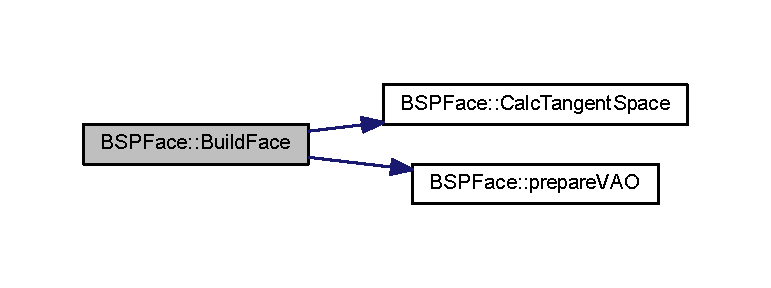
\includegraphics[width=350pt]{class_b_s_p_face_a4ae99df1fc45845b5a3049c73eb6ae25_cgraph}
\end{center}
\end{figure}




Here is the caller graph for this function\+:
\nopagebreak
\begin{figure}[H]
\begin{center}
\leavevmode
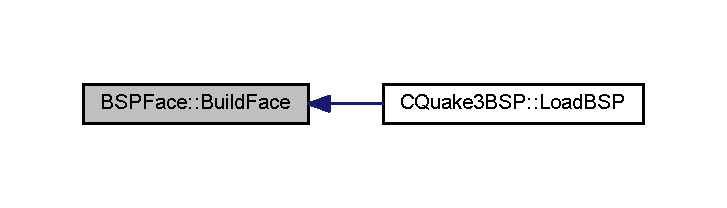
\includegraphics[width=349pt]{class_b_s_p_face_a4ae99df1fc45845b5a3049c73eb6ae25_icgraph}
\end{center}
\end{figure}


\index{B\+S\+P\+Face@{B\+S\+P\+Face}!Calc\+Tangent\+Space@{Calc\+Tangent\+Space}}
\index{Calc\+Tangent\+Space@{Calc\+Tangent\+Space}!B\+S\+P\+Face@{B\+S\+P\+Face}}
\subsubsection[{\texorpdfstring{Calc\+Tangent\+Space()}{CalcTangentSpace()}}]{\setlength{\rightskip}{0pt plus 5cm}bool B\+S\+P\+Face\+::\+Calc\+Tangent\+Space (
\begin{DoxyParamCaption}
{}
\end{DoxyParamCaption}
)\hspace{0.3cm}{\ttfamily [inline]}, {\ttfamily [private]}}\hypertarget{class_b_s_p_face_a5814b00d0169b2eb7808c0d64724dd94}{}\label{class_b_s_p_face_a5814b00d0169b2eb7808c0d64724dd94}
calculate tangent/bitangent vectors of both triangles

tangent1 = glm\+::normalize(tangent1);

bitangent1 = glm\+::normalize(bitangent1); 

Definition at line 93 of file B\+S\+P\+Face.\+h.



Here is the caller graph for this function\+:
\nopagebreak
\begin{figure}[H]
\begin{center}
\leavevmode
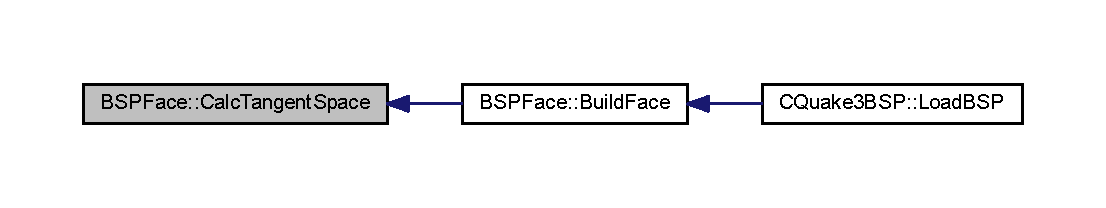
\includegraphics[width=350pt]{class_b_s_p_face_a5814b00d0169b2eb7808c0d64724dd94_icgraph}
\end{center}
\end{figure}


\index{B\+S\+P\+Face@{B\+S\+P\+Face}!prepare\+V\+AO@{prepare\+V\+AO}}
\index{prepare\+V\+AO@{prepare\+V\+AO}!B\+S\+P\+Face@{B\+S\+P\+Face}}
\subsubsection[{\texorpdfstring{prepare\+V\+A\+O()}{prepareVAO()}}]{\setlength{\rightskip}{0pt plus 5cm}bool B\+S\+P\+Face\+::prepare\+V\+AO (
\begin{DoxyParamCaption}
{}
\end{DoxyParamCaption}
)\hspace{0.3cm}{\ttfamily [inline]}, {\ttfamily [private]}}\hypertarget{class_b_s_p_face_a53ccd893ab6d659edb33fb09de00d7be}{}\label{class_b_s_p_face_a53ccd893ab6d659edb33fb09de00d7be}
Load data into vertex buffers

A great thing about structs is that their memory layout is sequential for all its items. The effect is that we can simply pass a pointer to the struct and it translates perfectly to a glm\+::vec3/2 array which again translates to 3/2 floats which translates to a byte array.

Set the vertex attribute pointers \hyperlink{struct_vertex}{Vertex} Positions

\hyperlink{struct_vertex}{Vertex} \hyperlink{struct_texture}{Texture} Coords

\hyperlink{struct_vertex}{Vertex} Normals

\hyperlink{struct_vertex}{Vertex} Tangent

\hyperlink{struct_vertex}{Vertex} Bitangent 

Definition at line 135 of file B\+S\+P\+Face.\+h.



Here is the caller graph for this function\+:
\nopagebreak
\begin{figure}[H]
\begin{center}
\leavevmode
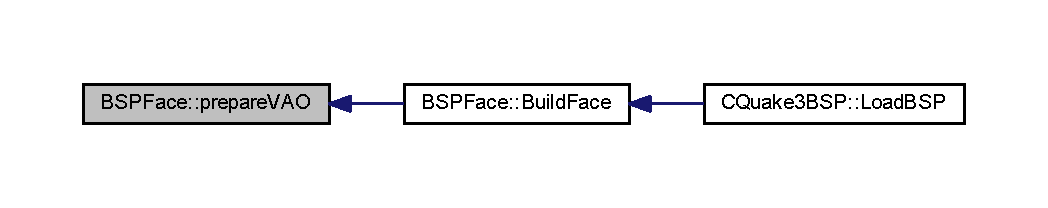
\includegraphics[width=350pt]{class_b_s_p_face_a53ccd893ab6d659edb33fb09de00d7be_icgraph}
\end{center}
\end{figure}



\hypertarget{class_b_s_pfile}{}\section{B\+S\+Pfile Class Reference}
\label{class_b_s_pfile}\index{B\+S\+Pfile@{B\+S\+Pfile}}


Collaboration diagram for B\+S\+Pfile\+:
\nopagebreak
\begin{figure}[H]
\begin{center}
\leavevmode
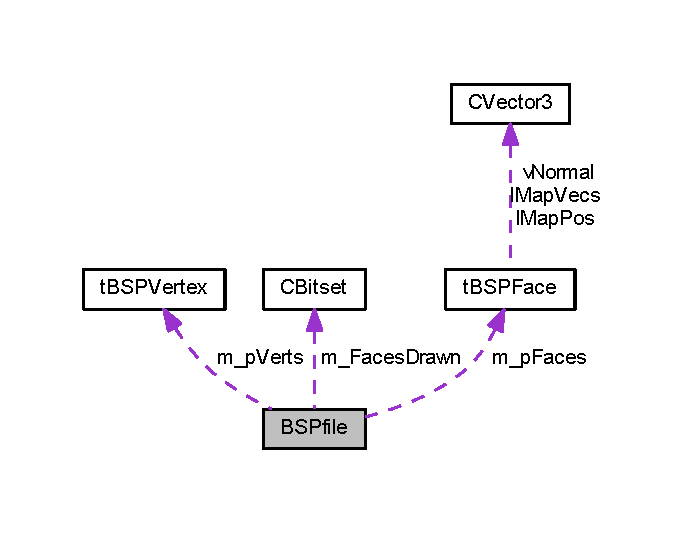
\includegraphics[width=329pt]{class_b_s_pfile__coll__graph}
\end{center}
\end{figure}
\subsection*{Public Member Functions}
\begin{DoxyCompactItemize}
\item 
bool \hyperlink{class_b_s_pfile_abfb2664873246b1714ffa17593cb6cf2}{Load\+B\+SP} (const char $\ast$str\+File\+Name)\hypertarget{class_b_s_pfile_abfb2664873246b1714ffa17593cb6cf2}{}\label{class_b_s_pfile_abfb2664873246b1714ffa17593cb6cf2}

\begin{DoxyCompactList}\small\item\em This loads a .bsp file by it\textquotesingle{}s file name (Returns true if successful) \end{DoxyCompactList}\item 
void \hyperlink{class_b_s_pfile_a7b15a3485081c1e8b31209271a68e0a6}{Render\+Level} (const glm\+::vec3 \&v\+Pos)\hypertarget{class_b_s_pfile_a7b15a3485081c1e8b31209271a68e0a6}{}\label{class_b_s_pfile_a7b15a3485081c1e8b31209271a68e0a6}

\begin{DoxyCompactList}\small\item\em This renders the level to the screen, currently the camera pos isn\textquotesingle{}t being used. \end{DoxyCompactList}\item 
void \hyperlink{class_b_s_pfile_a703bd45549f861ea4a84852538b0fcb1}{Destroy} ()\hypertarget{class_b_s_pfile_a703bd45549f861ea4a84852538b0fcb1}{}\label{class_b_s_pfile_a703bd45549f861ea4a84852538b0fcb1}

\begin{DoxyCompactList}\small\item\em This destroys the level data. \end{DoxyCompactList}\end{DoxyCompactItemize}
\subsection*{Private Member Functions}
\begin{DoxyCompactItemize}
\item 
void \hyperlink{class_b_s_pfile_ae1f8be78e62a72e8d38f5858bddb9c1b}{Find\+Texture\+Extension} (char $\ast$str\+File\+Name)\hypertarget{class_b_s_pfile_ae1f8be78e62a72e8d38f5858bddb9c1b}{}\label{class_b_s_pfile_ae1f8be78e62a72e8d38f5858bddb9c1b}

\begin{DoxyCompactList}\small\item\em This attaches the correct extension to the file name, if found. \end{DoxyCompactList}\item 
void \hyperlink{class_b_s_pfile_a25c51a5f92f9fe447dbbb1c33785c117}{Render\+Face} (int face\+Index)\hypertarget{class_b_s_pfile_a25c51a5f92f9fe447dbbb1c33785c117}{}\label{class_b_s_pfile_a25c51a5f92f9fe447dbbb1c33785c117}

\begin{DoxyCompactList}\small\item\em This renders a single face to the screen. \end{DoxyCompactList}\end{DoxyCompactItemize}
\subsection*{Private Attributes}
\begin{DoxyCompactItemize}
\item 
int {\bfseries m\+\_\+num\+Of\+Verts}\hypertarget{class_b_s_pfile_a4ace6677bd15bc1e1476f24e0c2864f1}{}\label{class_b_s_pfile_a4ace6677bd15bc1e1476f24e0c2864f1}

\item 
int \hyperlink{class_b_s_pfile_a12bfa8c7e0d985dd89193bce795f2613}{m\+\_\+num\+Of\+Faces}\hypertarget{class_b_s_pfile_a12bfa8c7e0d985dd89193bce795f2613}{}\label{class_b_s_pfile_a12bfa8c7e0d985dd89193bce795f2613}

\begin{DoxyCompactList}\small\item\em The number of verts in the model. \end{DoxyCompactList}\item 
int \hyperlink{class_b_s_pfile_a764cccbff1b8f80ef366f35c4edc721e}{m\+\_\+num\+Of\+Indices}\hypertarget{class_b_s_pfile_a764cccbff1b8f80ef366f35c4edc721e}{}\label{class_b_s_pfile_a764cccbff1b8f80ef366f35c4edc721e}

\begin{DoxyCompactList}\small\item\em The number of faces in the model. \end{DoxyCompactList}\item 
int \hyperlink{class_b_s_pfile_a862b3f1249427bcacf1ade8362b753c8}{m\+\_\+num\+Of\+Textures}\hypertarget{class_b_s_pfile_a862b3f1249427bcacf1ade8362b753c8}{}\label{class_b_s_pfile_a862b3f1249427bcacf1ade8362b753c8}

\begin{DoxyCompactList}\small\item\em The number of indices for the model. \end{DoxyCompactList}\item 
int $\ast$ \hyperlink{class_b_s_pfile_aa86af87121864c5cfef95e5278241f7b}{m\+\_\+p\+Indices}\hypertarget{class_b_s_pfile_aa86af87121864c5cfef95e5278241f7b}{}\label{class_b_s_pfile_aa86af87121864c5cfef95e5278241f7b}

\begin{DoxyCompactList}\small\item\em The number of texture maps. \end{DoxyCompactList}\item 
\hyperlink{structt_b_s_p_vertex}{t\+B\+S\+P\+Vertex} $\ast$ \hyperlink{class_b_s_pfile_a6ddf2eae40c66dad1e2306aab2b79c4b}{m\+\_\+p\+Verts}\hypertarget{class_b_s_pfile_a6ddf2eae40c66dad1e2306aab2b79c4b}{}\label{class_b_s_pfile_a6ddf2eae40c66dad1e2306aab2b79c4b}

\begin{DoxyCompactList}\small\item\em The object\textquotesingle{}s indices for rendering. \end{DoxyCompactList}\item 
\hyperlink{structt_b_s_p_face}{t\+B\+S\+P\+Face} $\ast$ \hyperlink{class_b_s_pfile_a229bf352e07fe5fc205925ef4bcd204c}{m\+\_\+p\+Faces}\hypertarget{class_b_s_pfile_a229bf352e07fe5fc205925ef4bcd204c}{}\label{class_b_s_pfile_a229bf352e07fe5fc205925ef4bcd204c}

\begin{DoxyCompactList}\small\item\em The object\textquotesingle{}s vertices. \end{DoxyCompactList}\item 
unsigned int \hyperlink{class_b_s_pfile_ade4ec8b0582ac55d498ce1d53b94a565}{m\+\_\+textures} \mbox{[}500\mbox{]}
\begin{DoxyCompactList}\small\item\em The texture and lightmap array for the level. \end{DoxyCompactList}\item 
\hyperlink{class_c_bitset}{C\+Bitset} {\bfseries m\+\_\+\+Faces\+Drawn}\hypertarget{class_b_s_pfile_a500f3a4700116398f61dcca78ceca484}{}\label{class_b_s_pfile_a500f3a4700116398f61dcca78ceca484}

\end{DoxyCompactItemize}


\subsection{Detailed Description}
========= Copyright Survtech, All rights reserved. ============//

Purpose\+: 

 

Definition at line 19 of file B\+S\+Pfile.\+h.



\subsection{Field Documentation}
\index{B\+S\+Pfile@{B\+S\+Pfile}!m\+\_\+textures@{m\+\_\+textures}}
\index{m\+\_\+textures@{m\+\_\+textures}!B\+S\+Pfile@{B\+S\+Pfile}}
\subsubsection[{\texorpdfstring{m\+\_\+textures}{m_textures}}]{\setlength{\rightskip}{0pt plus 5cm}unsigned int B\+S\+Pfile\+::m\+\_\+textures\mbox{[}500\mbox{]}\hspace{0.3cm}{\ttfamily [private]}}\hypertarget{class_b_s_pfile_ade4ec8b0582ac55d498ce1d53b94a565}{}\label{class_b_s_pfile_ade4ec8b0582ac55d498ce1d53b94a565}


The texture and lightmap array for the level. 

The faces information of the object 

Definition at line 52 of file B\+S\+Pfile.\+h.


\hypertarget{struct_b_s_p_texture}{}\section{B\+S\+P\+Texture Struct Reference}
\label{struct_b_s_p_texture}\index{B\+S\+P\+Texture@{B\+S\+P\+Texture}}


Collaboration diagram for B\+S\+P\+Texture\+:
\nopagebreak
\begin{figure}[H]
\begin{center}
\leavevmode
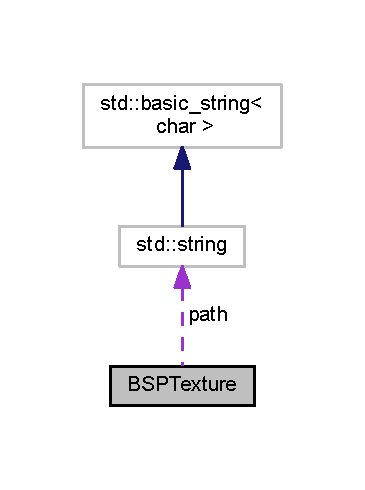
\includegraphics[width=175pt]{struct_b_s_p_texture__coll__graph}
\end{center}
\end{figure}
\subsection*{Data Fields}
\begin{DoxyCompactItemize}
\item 
string {\bfseries path}\hypertarget{struct_b_s_p_texture_a6224e57403bbc640af1d4bb0d0f1a15a}{}\label{struct_b_s_p_texture_a6224e57403bbc640af1d4bb0d0f1a15a}

\item 
G\+Luint {\bfseries G\+L\+Texture\+ID}\hypertarget{struct_b_s_p_texture_aa267445bc116004d7cd7196e0b01e567}{}\label{struct_b_s_p_texture_aa267445bc116004d7cd7196e0b01e567}

\item 
int {\bfseries type}\hypertarget{struct_b_s_p_texture_a2617bf848d7df3492c45341e474fff5e}{}\label{struct_b_s_p_texture_a2617bf848d7df3492c45341e474fff5e}

\end{DoxyCompactItemize}


\subsection{Detailed Description}


Definition at line 93 of file B\+S\+P.\+h.


\hypertarget{class_button}{}\section{Button Class Reference}
\label{class_button}\index{Button@{Button}}


Inheritance diagram for Button\+:
\nopagebreak
\begin{figure}[H]
\begin{center}
\leavevmode
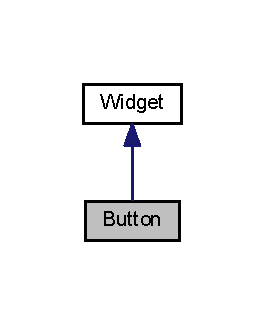
\includegraphics[width=127pt]{class_button__inherit__graph}
\end{center}
\end{figure}


Collaboration diagram for Button\+:
\nopagebreak
\begin{figure}[H]
\begin{center}
\leavevmode
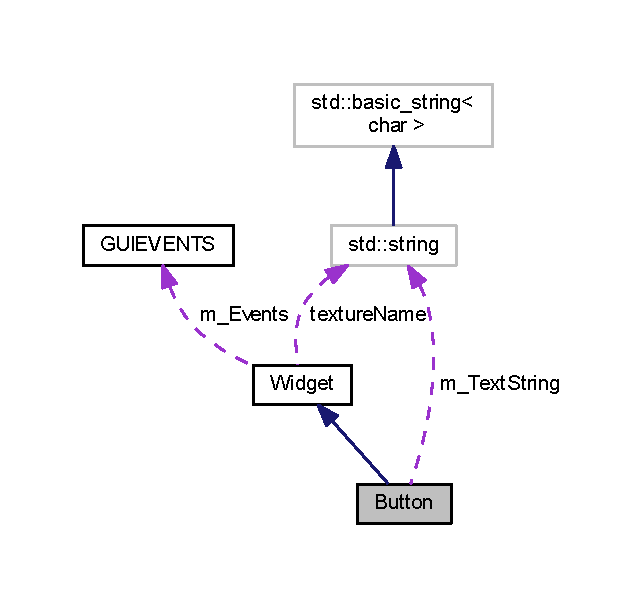
\includegraphics[width=309pt]{class_button__coll__graph}
\end{center}
\end{figure}
\subsection*{Public Member Functions}
\begin{DoxyCompactItemize}
\item 
{\bfseries Button} (float width, float height, int win\+Width, int win\+Height, std\+::string text)\hypertarget{class_button_ac9e452a0f12897a81fd5e052176aeaf6}{}\label{class_button_ac9e452a0f12897a81fd5e052176aeaf6}

\item 
void {\bfseries Render} (std\+::shared\+\_\+ptr$<$ \hyperlink{class_shader}{Shader} $>$ shader)\hypertarget{class_button_a746cc4d16abaf65168806b3b1505c011}{}\label{class_button_a746cc4d16abaf65168806b3b1505c011}

\item 
void {\bfseries Update} ()\hypertarget{class_button_a23e8bc9ad05142244ea4e79a406a6c9c}{}\label{class_button_a23e8bc9ad05142244ea4e79a406a6c9c}

\end{DoxyCompactItemize}
\subsection*{Data Fields}
\begin{DoxyCompactItemize}
\item 
std\+::shared\+\_\+ptr$<$ \hyperlink{class_text}{Text} $>$ {\bfseries m\+\_\+\+Text\+Renderer\+Instance}\hypertarget{class_button_afc58e980e856ef0a9f5835846261e751}{}\label{class_button_afc58e980e856ef0a9f5835846261e751}

\end{DoxyCompactItemize}
\subsection*{Private Attributes}
\begin{DoxyCompactItemize}
\item 
float {\bfseries m\+\_\+\+Opacity}\hypertarget{class_button_a65236f721197446602505157028da626}{}\label{class_button_a65236f721197446602505157028da626}

\item 
float {\bfseries m\+\_\+\+Width}\hypertarget{class_button_abb91d7816eb9610ccea86bd7998fa4d2}{}\label{class_button_abb91d7816eb9610ccea86bd7998fa4d2}

\item 
float {\bfseries m\+\_\+\+Height}\hypertarget{class_button_a566dc820d67b7a77441ad07170e1eb75}{}\label{class_button_a566dc820d67b7a77441ad07170e1eb75}

\item 
float {\bfseries m\+\_\+win\+Width}\hypertarget{class_button_a23c34faf74b886dd7ec9c8eca67e466b}{}\label{class_button_a23c34faf74b886dd7ec9c8eca67e466b}

\item 
float {\bfseries m\+\_\+win\+Height}\hypertarget{class_button_a0682411e09402316a1d362d66298f41b}{}\label{class_button_a0682411e09402316a1d362d66298f41b}

\item 
float {\bfseries m\+\_\+text\+Width} = 0.\+0\hypertarget{class_button_ac4d2a5749af6b990e708bd1f062aad3c}{}\label{class_button_ac4d2a5749af6b990e708bd1f062aad3c}

\item 
float {\bfseries m\+\_\+text\+Height} = 0.\+0\hypertarget{class_button_a71a4ddbb20ad2bdea2de33ebac659670}{}\label{class_button_a71a4ddbb20ad2bdea2de33ebac659670}

\item 
glm\+::mat4 {\bfseries projection}\hypertarget{class_button_ab210a540cfa946560ab6e2dd2f5aa9f3}{}\label{class_button_ab210a540cfa946560ab6e2dd2f5aa9f3}

\item 
std\+::shared\+\_\+ptr$<$ \hyperlink{class_open_g_l_helpers_1_1_quad}{Open\+G\+L\+Helpers\+::\+Quad} $>$ {\bfseries m\+\_\+\+Quad}\hypertarget{class_button_a3b1bf861e58dadc97e1554b141b2cb13}{}\label{class_button_a3b1bf861e58dadc97e1554b141b2cb13}

\item 
std\+::string {\bfseries m\+\_\+\+Text\+String}\hypertarget{class_button_af0132736c89e3da304cac4a5ec8d8c02}{}\label{class_button_af0132736c89e3da304cac4a5ec8d8c02}

\end{DoxyCompactItemize}
\subsection*{Additional Inherited Members}


\subsection{Detailed Description}


Definition at line 7 of file Button.\+h.


\hypertarget{class_camera}{}\section{Camera Class Reference}
\label{class_camera}\index{Camera@{Camera}}
\subsection*{Public Member Functions}
\begin{DoxyCompactItemize}
\item 
{\bfseries Camera} (glm\+::vec3, glm\+::vec3)\hypertarget{class_camera_a7ac99ca06250df56ae81414fe54589e2}{}\label{class_camera_a7ac99ca06250df56ae81414fe54589e2}

\item 
void {\bfseries Update} (G\+L\+F\+Wwindow $\ast$\&)\hypertarget{class_camera_a0d9114c1c4de87842d227d511e045df5}{}\label{class_camera_a0d9114c1c4de87842d227d511e045df5}

\item 
void {\bfseries Update\+Matrices} (void)\hypertarget{class_camera_acdf18835a138363721f33a6d3bf085b2}{}\label{class_camera_acdf18835a138363721f33a6d3bf085b2}

\item 
glm\+::mat4 {\bfseries get\+View\+Matrix} (void)\hypertarget{class_camera_a5b68da2e7a27893a7a3a8ac85c5b788f}{}\label{class_camera_a5b68da2e7a27893a7a3a8ac85c5b788f}

\item 
glm\+::mat4 {\bfseries get\+Prev\+View\+Matrix} (void)\hypertarget{class_camera_a8566bc0b2a61fc6d74995f2dc4ea8017}{}\label{class_camera_a8566bc0b2a61fc6d74995f2dc4ea8017}

\item 
glm\+::mat4 {\bfseries get\+Projection\+Matrix} (void)\hypertarget{class_camera_a2ebb2fdd189345caa39113fcafcc6d5a}{}\label{class_camera_a2ebb2fdd189345caa39113fcafcc6d5a}

\item 
glm\+::vec3 {\bfseries get\+Position} (void)\hypertarget{class_camera_a0a32173c1f61b10ced8f674758872403}{}\label{class_camera_a0a32173c1f61b10ced8f674758872403}

\item 
glm\+::vec3 {\bfseries get\+Direction} (void)\hypertarget{class_camera_a50f87cd85fd230c6b5196e552c4fe45f}{}\label{class_camera_a50f87cd85fd230c6b5196e552c4fe45f}

\item 
glm\+::vec3 {\bfseries get\+Up} (void)\hypertarget{class_camera_ae3b6ae9df4f8003f7985e683a375899c}{}\label{class_camera_ae3b6ae9df4f8003f7985e683a375899c}

\item 
glm\+::vec3 {\bfseries get\+Right} (void)\hypertarget{class_camera_aa4797845d8c2179a0ad9d47a32e1abd5}{}\label{class_camera_aa4797845d8c2179a0ad9d47a32e1abd5}

\item 
void {\bfseries set\+Position} (glm\+::vec3 new\+Position)\hypertarget{class_camera_aac2d0a2bd337c4523d38aefbdaeb8d41}{}\label{class_camera_aac2d0a2bd337c4523d38aefbdaeb8d41}

\item 
void {\bfseries set\+Direction} (glm\+::vec3 new\+Direction)\hypertarget{class_camera_ae871e4e4e8903f77897fdcb911a3642e}{}\label{class_camera_ae871e4e4e8903f77897fdcb911a3642e}

\item 
void {\bfseries set\+FoV} (float FoV)\hypertarget{class_camera_ade678831d00089b370b08e71c81f5215}{}\label{class_camera_ade678831d00089b370b08e71c81f5215}

\item 
float {\bfseries get\+FoV} ()\hypertarget{class_camera_aef7933e312710e4ed87329dbabb15a99}{}\label{class_camera_aef7933e312710e4ed87329dbabb15a99}

\item 
void {\bfseries set\+Projection} (float F\+OV, float AR, float N\+E\+AR, float F\+AR)\hypertarget{class_camera_a1956749dfc92f5b9c75bcff120e8ab5a}{}\label{class_camera_a1956749dfc92f5b9c75bcff120e8ab5a}

\item 
void {\bfseries set\+Projection} (glm\+::mat4)\hypertarget{class_camera_aa1606d668b24df804e1e4358040caa7f}{}\label{class_camera_aa1606d668b24df804e1e4358040caa7f}

\item 
void {\bfseries set\+View\+Matrix} (glm\+::mat4)\hypertarget{class_camera_abb039add28392d053bbc0759afee84f7}{}\label{class_camera_abb039add28392d053bbc0759afee84f7}

\item 
bool {\bfseries is\+Moving} ()\hypertarget{class_camera_ae5e581022eba09a62f7e8dde90dd17b0}{}\label{class_camera_ae5e581022eba09a62f7e8dde90dd17b0}

\end{DoxyCompactItemize}
\subsection*{Data Fields}
\begin{DoxyCompactItemize}
\item 
glm\+::mat4 {\bfseries M\+VP}\hypertarget{class_camera_acbffeb464f0d15fa92f6780ef1e005d7}{}\label{class_camera_acbffeb464f0d15fa92f6780ef1e005d7}

\item 
float {\bfseries Movement\+Speed}\hypertarget{class_camera_a63221392d762df6a74f45bc9d43a2f61}{}\label{class_camera_a63221392d762df6a74f45bc9d43a2f61}

\item 
float {\bfseries Mouse\+Speed}\hypertarget{class_camera_a54fc599f1742077bbc84f623a23112ae}{}\label{class_camera_a54fc599f1742077bbc84f623a23112ae}

\item 
float {\bfseries Joystick\+Sensibility}\hypertarget{class_camera_af5985750a20cb55024671cf61b8f6c4a}{}\label{class_camera_af5985750a20cb55024671cf61b8f6c4a}

\item 
float {\bfseries Field\+Of\+View}\hypertarget{class_camera_aa58ac7abca90e0a182493b86f7b1c4d2}{}\label{class_camera_aa58ac7abca90e0a182493b86f7b1c4d2}

\item 
int {\bfseries winx}\hypertarget{class_camera_acb5a9b01adbd32a00e5d70c4f175c467}{}\label{class_camera_acb5a9b01adbd32a00e5d70c4f175c467}

\item 
int {\bfseries winy}\hypertarget{class_camera_a94f986f9ed4b4a07f2d9ee857d958b32}{}\label{class_camera_a94f986f9ed4b4a07f2d9ee857d958b32}

\item 
float {\bfseries Max\+Movement\+Speed}\hypertarget{class_camera_a161269518cec25e3597455472610a311}{}\label{class_camera_a161269518cec25e3597455472610a311}

\item 
bool {\bfseries m\+Is\+Moving} = false\hypertarget{class_camera_a0138317fb414868490876f0d23ef5ff3}{}\label{class_camera_a0138317fb414868490876f0d23ef5ff3}

\end{DoxyCompactItemize}
\subsection*{Private Member Functions}
\begin{DoxyCompactItemize}
\item 
void {\bfseries Lock\+Camera} (void)\hypertarget{class_camera_abff5b93c71289be007f966060ff9a70d}{}\label{class_camera_abff5b93c71289be007f966060ff9a70d}

\item 
void \hyperlink{class_camera_a63bf578388a6ea87d2d0a250f91198ab}{Handle\+Inputs} (G\+L\+F\+Wwindow $\ast$\&)
\item 
void {\bfseries Get\+External\+Inputs} (void)\hypertarget{class_camera_ae26cc8359a03e57b9f26c149574e920d}{}\label{class_camera_ae26cc8359a03e57b9f26c149574e920d}

\end{DoxyCompactItemize}
\subsection*{Private Attributes}
\begin{DoxyCompactItemize}
\item 
glm\+::vec3 {\bfseries Rigth}\hypertarget{class_camera_a3b7666cf3dbaf02534a2644abaa5be76}{}\label{class_camera_a3b7666cf3dbaf02534a2644abaa5be76}

\item 
glm\+::vec3 {\bfseries Up}\hypertarget{class_camera_ad74c4a490bc8865e67e27a2036d0a72d}{}\label{class_camera_ad74c4a490bc8865e67e27a2036d0a72d}

\item 
glm\+::vec3 {\bfseries Frustrum}\hypertarget{class_camera_ae18be48fbe18e69438525168435bc745}{}\label{class_camera_ae18be48fbe18e69438525168435bc745}

\item 
glm\+::vec3 {\bfseries new\+Orientation}\hypertarget{class_camera_a0781b6d41623d8798e92a25151ff3cd8}{}\label{class_camera_a0781b6d41623d8798e92a25151ff3cd8}

\item 
glm\+::vec3 {\bfseries new\+Position}\hypertarget{class_camera_ab80cd05699e81ec019e256b2f1c07d3e}{}\label{class_camera_ab80cd05699e81ec019e256b2f1c07d3e}

\item 
glm\+::mat4 {\bfseries Prev\+View}\hypertarget{class_camera_a2f4f0321841106b34b9faa9a222580bc}{}\label{class_camera_a2f4f0321841106b34b9faa9a222580bc}

\item 
bool {\bfseries Orientationhas\+Changed}\hypertarget{class_camera_a73bb980786eb9ee9e23ad99ee06c3907}{}\label{class_camera_a73bb980786eb9ee9e23ad99ee06c3907}

\item 
bool {\bfseries Positionhas\+Changed}\hypertarget{class_camera_acc8ddad12bc8d2d6289df0884cfa9a9e}{}\label{class_camera_acc8ddad12bc8d2d6289df0884cfa9a9e}

\item 
float {\bfseries vertical\+Angle}\hypertarget{class_camera_a6582a5068d81b8de7a7fc67e5143e628}{}\label{class_camera_a6582a5068d81b8de7a7fc67e5143e628}

\item 
float {\bfseries horizontal\+Angle}\hypertarget{class_camera_aad9d573147be409e929251eca0bea339}{}\label{class_camera_aad9d573147be409e929251eca0bea339}

\item 
glm\+::mat4 {\bfseries View\+Matrix}\hypertarget{class_camera_a34f22e4635ee38206e4b9c59095d43bf}{}\label{class_camera_a34f22e4635ee38206e4b9c59095d43bf}

\item 
glm\+::mat4 {\bfseries Projection\+Matrix}\hypertarget{class_camera_a8f5424b6795715c8a44805d1c3a5b11c}{}\label{class_camera_a8f5424b6795715c8a44805d1c3a5b11c}

\item 
glm\+::vec3 {\bfseries Position}\hypertarget{class_camera_a9733b59f5340f6f1bca24d52a6679039}{}\label{class_camera_a9733b59f5340f6f1bca24d52a6679039}

\item 
glm\+::vec3 {\bfseries Orientation}\hypertarget{class_camera_ab998c79a8bcbd71dcaad201f536e36e1}{}\label{class_camera_ab998c79a8bcbd71dcaad201f536e36e1}

\item 
glm\+::vec3 {\bfseries Last\+Position}\hypertarget{class_camera_a274def711ceb63556a3074da11fb43df}{}\label{class_camera_a274def711ceb63556a3074da11fb43df}

\item 
glm\+::vec3 {\bfseries Delta\+Vector}\hypertarget{class_camera_a92ea5380dd9962b451e067fe1c3c81dc}{}\label{class_camera_a92ea5380dd9962b451e067fe1c3c81dc}

\item 
glm\+::vec3 {\bfseries Movement\+Vector}\hypertarget{class_camera_a0d450752f3639989bc813bb077dd9f13}{}\label{class_camera_a0d450752f3639989bc813bb077dd9f13}

\end{DoxyCompactItemize}


\subsection{Detailed Description}
========= Copyright Survtech, All rights reserved. ============//

Purpose\+: 

 

Definition at line 16 of file camera.\+h.



\subsection{Member Function Documentation}
\index{Camera@{Camera}!Handle\+Inputs@{Handle\+Inputs}}
\index{Handle\+Inputs@{Handle\+Inputs}!Camera@{Camera}}
\subsubsection[{\texorpdfstring{Handle\+Inputs(\+G\+L\+F\+Wwindow $\ast$\&)}{HandleInputs(GLFWwindow *&)}}]{\setlength{\rightskip}{0pt plus 5cm}void Camera\+::\+Handle\+Inputs (
\begin{DoxyParamCaption}
\item[{G\+L\+F\+Wwindow $\ast$\&}]{window}
\end{DoxyParamCaption}
)\hspace{0.3cm}{\ttfamily [private]}}\hypertarget{class_camera_a63bf578388a6ea87d2d0a250f91198ab}{}\label{class_camera_a63bf578388a6ea87d2d0a250f91198ab}
Keyboard \hyperlink{class_camera}{Camera} input 



Joystick \hyperlink{class_camera}{Camera} input 



Definition at line 73 of file Camera.\+cpp.


\hypertarget{class_c_bitset}{}\section{C\+Bitset Class Reference}
\label{class_c_bitset}\index{C\+Bitset@{C\+Bitset}}
\subsection*{Public Member Functions}
\begin{DoxyCompactItemize}
\item 
void {\bfseries Resize} (int count)\hypertarget{class_c_bitset_a452780d0a5bf716012e7706929885a27}{}\label{class_c_bitset_a452780d0a5bf716012e7706929885a27}

\item 
void {\bfseries Set} (int i)\hypertarget{class_c_bitset_a217900efa644dd8d739a756d6811e475}{}\label{class_c_bitset_a217900efa644dd8d739a756d6811e475}

\item 
int {\bfseries On} (int i)\hypertarget{class_c_bitset_a57dfc60d4a180f8166e94bd41612d3f8}{}\label{class_c_bitset_a57dfc60d4a180f8166e94bd41612d3f8}

\item 
void {\bfseries Clear} (int i)\hypertarget{class_c_bitset_a0278f6027f4bbc3177731ccadb638e2a}{}\label{class_c_bitset_a0278f6027f4bbc3177731ccadb638e2a}

\item 
void {\bfseries Clear\+All} ()\hypertarget{class_c_bitset_ad1cf97399375c29574079338ce02d7ac}{}\label{class_c_bitset_ad1cf97399375c29574079338ce02d7ac}

\item 
\hyperlink{class_c_bitset_a20e9448086472dcf6cba08abf8a55f0a}{C\+Bitset} ()\hypertarget{class_c_bitset_a20e9448086472dcf6cba08abf8a55f0a}{}\label{class_c_bitset_a20e9448086472dcf6cba08abf8a55f0a}

\begin{DoxyCompactList}\small\item\em Initialize all the data members. \end{DoxyCompactList}\item 
\hyperlink{class_c_bitset_a9332c709c4d655959bcdac749db593b4}{$\sim$\+C\+Bitset} ()
\begin{DoxyCompactList}\small\item\em This is our deconstructor. \end{DoxyCompactList}\item 
void \hyperlink{class_c_bitset_a452780d0a5bf716012e7706929885a27}{Resize} (int count)
\begin{DoxyCompactList}\small\item\em This resizes our bitset to a size so each face has a bit associated with it. \end{DoxyCompactList}\item 
void \hyperlink{class_c_bitset_a217900efa644dd8d739a756d6811e475}{Set} (int i)\hypertarget{class_c_bitset_a217900efa644dd8d739a756d6811e475}{}\label{class_c_bitset_a217900efa644dd8d739a756d6811e475}

\begin{DoxyCompactList}\small\item\em This does the binary math to set the desired bit. \end{DoxyCompactList}\item 
int \hyperlink{class_c_bitset_a57dfc60d4a180f8166e94bd41612d3f8}{On} (int i)\hypertarget{class_c_bitset_a57dfc60d4a180f8166e94bd41612d3f8}{}\label{class_c_bitset_a57dfc60d4a180f8166e94bd41612d3f8}

\begin{DoxyCompactList}\small\item\em This returns if the desired bit slot is a 1 or a 0. \end{DoxyCompactList}\item 
void \hyperlink{class_c_bitset_a0278f6027f4bbc3177731ccadb638e2a}{Clear} (int i)\hypertarget{class_c_bitset_a0278f6027f4bbc3177731ccadb638e2a}{}\label{class_c_bitset_a0278f6027f4bbc3177731ccadb638e2a}

\begin{DoxyCompactList}\small\item\em This clears a bit to 0. \end{DoxyCompactList}\item 
void \hyperlink{class_c_bitset_ad1cf97399375c29574079338ce02d7ac}{Clear\+All} ()\hypertarget{class_c_bitset_ad1cf97399375c29574079338ce02d7ac}{}\label{class_c_bitset_ad1cf97399375c29574079338ce02d7ac}

\begin{DoxyCompactList}\small\item\em This initializes the bits to 0. \end{DoxyCompactList}\end{DoxyCompactItemize}
\subsection*{Private Attributes}
\begin{DoxyCompactItemize}
\item 
unsigned int $\ast$ \hyperlink{class_c_bitset_ad652e9601865e54acd0d956b1493a535}{m\+\_\+bits}\hypertarget{class_c_bitset_ad652e9601865e54acd0d956b1493a535}{}\label{class_c_bitset_ad652e9601865e54acd0d956b1493a535}

\begin{DoxyCompactList}\small\item\em Our private bit data that holds the bits and size. \end{DoxyCompactList}\item 
int {\bfseries m\+\_\+size}\hypertarget{class_c_bitset_ab55d8030981a04787e0198a124fa8488}{}\label{class_c_bitset_ab55d8030981a04787e0198a124fa8488}

\end{DoxyCompactItemize}


\subsection{Detailed Description}
========= Copyright Survtech, All rights reserved. ============//

Purpose\+: 

 

Definition at line 164 of file B\+S\+P.\+h.



\subsection{Constructor \& Destructor Documentation}
\index{C\+Bitset@{C\+Bitset}!````~C\+Bitset@{$\sim$\+C\+Bitset}}
\index{````~C\+Bitset@{$\sim$\+C\+Bitset}!C\+Bitset@{C\+Bitset}}
\subsubsection[{\texorpdfstring{$\sim$\+C\+Bitset()}{~CBitset()}}]{\setlength{\rightskip}{0pt plus 5cm}C\+Bitset\+::$\sim$\+C\+Bitset (
\begin{DoxyParamCaption}
{}
\end{DoxyParamCaption}
)\hspace{0.3cm}{\ttfamily [inline]}}\hypertarget{class_c_bitset_a9332c709c4d655959bcdac749db593b4}{}\label{class_c_bitset_a9332c709c4d655959bcdac749db593b4}


This is our deconstructor. 

If we have valid memory, get rid of it 

Definition at line 25 of file C\+Bitset.\+h.



\subsection{Member Function Documentation}
\index{C\+Bitset@{C\+Bitset}!Resize@{Resize}}
\index{Resize@{Resize}!C\+Bitset@{C\+Bitset}}
\subsubsection[{\texorpdfstring{Resize(int count)}{Resize(int count)}}]{\setlength{\rightskip}{0pt plus 5cm}void C\+Bitset\+::\+Resize (
\begin{DoxyParamCaption}
\item[{int}]{count}
\end{DoxyParamCaption}
)\hspace{0.3cm}{\ttfamily [inline]}}\hypertarget{class_c_bitset_a452780d0a5bf716012e7706929885a27}{}\label{class_c_bitset_a452780d0a5bf716012e7706929885a27}


This resizes our bitset to a size so each face has a bit associated with it. 

Get the size of integers we need

Make sure we haven\textquotesingle{}t already allocated memory for the bits

Allocate the bits and initialize them 

Definition at line 36 of file C\+Bitset.\+h.


\hypertarget{class_c_frustum}{}\section{C\+Frustum Class Reference}
\label{class_c_frustum}\index{C\+Frustum@{C\+Frustum}}
\subsection*{Public Member Functions}
\begin{DoxyCompactItemize}
\item 
void \hyperlink{class_c_frustum_a9c1738062b94376ab2b754bfd6b4c363}{Calculate\+Frustum} (glm\+::mat4 Projection\+Matrix, glm\+::mat4 Model\+Matrix)
\item 
bool \hyperlink{class_c_frustum_aff4dd14b8d2528621030756d21e37d7f}{Point\+In\+Frustum} (float x, float y, float z)
\item 
bool \hyperlink{class_c_frustum_af05ef901019c29f46d145c6ebe6ea62c}{Sphere\+In\+Frustum} (float x, float y, float z, float radius)
\item 
bool \hyperlink{class_c_frustum_a02d4b3e95c33f9f83fc4104a3f5363e5}{Cube\+In\+Frustum} (float x, float y, float z, float size)
\item 
bool \hyperlink{class_c_frustum_a06155e722ef85cce62f65d8667cf41fb}{Box\+In\+Frustum} (float x, float y, float z, float sizeX, float sizeY, float sizeZ)
\item 
bool \hyperlink{class_c_frustum_a34e0f4eee50fa86ab4dfbdb2b1a78264}{Box\+In\+Frustum} (\hyperlink{struct_m_i_n___m_a_x___p_o_i_n_t_s}{M\+I\+N\+\_\+\+M\+A\+X\+\_\+\+P\+O\+I\+N\+TS} points)
\end{DoxyCompactItemize}
\subsection*{Private Attributes}
\begin{DoxyCompactItemize}
\item 
float {\bfseries m\+\_\+\+Frustum} \mbox{[}6\mbox{]}\mbox{[}4\mbox{]} = \{\{1\}, \{1\}\}\hypertarget{class_c_frustum_a2673b79facea7c41014cc9afdd7af138}{}\label{class_c_frustum_a2673b79facea7c41014cc9afdd7af138}

\end{DoxyCompactItemize}


\subsection{Detailed Description}


Definition at line 7 of file Frustum.\+h.



\subsection{Member Function Documentation}
\index{C\+Frustum@{C\+Frustum}!Box\+In\+Frustum@{Box\+In\+Frustum}}
\index{Box\+In\+Frustum@{Box\+In\+Frustum}!C\+Frustum@{C\+Frustum}}
\subsubsection[{\texorpdfstring{Box\+In\+Frustum(float x, float y, float z, float size\+X, float size\+Y, float size\+Z)}{BoxInFrustum(float x, float y, float z, float sizeX, float sizeY, float sizeZ)}}]{\setlength{\rightskip}{0pt plus 5cm}bool C\+Frustum\+::\+Box\+In\+Frustum (
\begin{DoxyParamCaption}
\item[{float}]{x, }
\item[{float}]{y, }
\item[{float}]{z, }
\item[{float}]{sizeX, }
\item[{float}]{sizeY, }
\item[{float}]{sizeZ}
\end{DoxyParamCaption}
)}\hypertarget{class_c_frustum_a06155e722ef85cce62f65d8667cf41fb}{}\label{class_c_frustum_a06155e722ef85cce62f65d8667cf41fb}
Go through all of the corners of the box and check then again each plane in the frustum. If all of them are behind one of the planes, then it most like is not in the frustum.

If we get here, it isn\textquotesingle{}t in the frustum 

Definition at line 282 of file Frustum.\+cpp.

\index{C\+Frustum@{C\+Frustum}!Box\+In\+Frustum@{Box\+In\+Frustum}}
\index{Box\+In\+Frustum@{Box\+In\+Frustum}!C\+Frustum@{C\+Frustum}}
\subsubsection[{\texorpdfstring{Box\+In\+Frustum(\+M\+I\+N\+\_\+\+M\+A\+X\+\_\+\+P\+O\+I\+N\+T\+S points)}{BoxInFrustum(MIN_MAX_POINTS points)}}]{\setlength{\rightskip}{0pt plus 5cm}bool C\+Frustum\+::\+Box\+In\+Frustum (
\begin{DoxyParamCaption}
\item[{{\bf M\+I\+N\+\_\+\+M\+A\+X\+\_\+\+P\+O\+I\+N\+TS}}]{points}
\end{DoxyParamCaption}
)}\hypertarget{class_c_frustum_a34e0f4eee50fa86ab4dfbdb2b1a78264}{}\label{class_c_frustum_a34e0f4eee50fa86ab4dfbdb2b1a78264}
Go through all of the corners of the box and check then again each plane in the frustum. If all of them are behind one of the planes, then it most like is not in the frustum.

If we get here, it isn\textquotesingle{}t in the frustum 

Definition at line 306 of file Frustum.\+cpp.

\index{C\+Frustum@{C\+Frustum}!Calculate\+Frustum@{Calculate\+Frustum}}
\index{Calculate\+Frustum@{Calculate\+Frustum}!C\+Frustum@{C\+Frustum}}
\subsubsection[{\texorpdfstring{Calculate\+Frustum(glm\+::mat4 Projection\+Matrix, glm\+::mat4 Model\+Matrix)}{CalculateFrustum(glm::mat4 ProjectionMatrix, glm::mat4 ModelMatrix)}}]{\setlength{\rightskip}{0pt plus 5cm}void C\+Frustum\+::\+Calculate\+Frustum (
\begin{DoxyParamCaption}
\item[{glm\+::mat4}]{Projection\+Matrix, }
\item[{glm\+::mat4}]{Model\+Matrix}
\end{DoxyParamCaption}
)}\hypertarget{class_c_frustum_a9c1738062b94376ab2b754bfd6b4c363}{}\label{class_c_frustum_a9c1738062b94376ab2b754bfd6b4c363}
Normalize the B\+O\+T\+T\+OM side

This will extract the T\+OP side of the frustum

Normalize the T\+OP side

This will extract the B\+A\+CK side of the frustum

Normalize the B\+A\+CK side

Normalize the F\+R\+O\+NT side 

Definition at line 67 of file Frustum.\+cpp.

\index{C\+Frustum@{C\+Frustum}!Cube\+In\+Frustum@{Cube\+In\+Frustum}}
\index{Cube\+In\+Frustum@{Cube\+In\+Frustum}!C\+Frustum@{C\+Frustum}}
\subsubsection[{\texorpdfstring{Cube\+In\+Frustum(float x, float y, float z, float size)}{CubeInFrustum(float x, float y, float z, float size)}}]{\setlength{\rightskip}{0pt plus 5cm}bool C\+Frustum\+::\+Cube\+In\+Frustum (
\begin{DoxyParamCaption}
\item[{float}]{x, }
\item[{float}]{y, }
\item[{float}]{z, }
\item[{float}]{size}
\end{DoxyParamCaption}
)}\hypertarget{class_c_frustum_a02d4b3e95c33f9f83fc4104a3f5363e5}{}\label{class_c_frustum_a02d4b3e95c33f9f83fc4104a3f5363e5}
Basically, what is going on is, that we are given the center of the cube, and half the length. Think of it like a radius. Then we checking each point in the cube and seeing if it is inside the frustum. If a point is found in front of a side, then we skip to the next side. If we get to a plane that does N\+OT have a point in front of it, then it will return false.

{\itshape Note} -\/ This will sometimes say that a cube is inside the frustum when it isn\textquotesingle{}t. This happens when all the corners of the bounding box are not behind any one plane. This is rare and shouldn\textquotesingle{}t effect the overall rendering speed.

If we get here, it isn\textquotesingle{}t in the frustum 

Definition at line 236 of file Frustum.\+cpp.

\index{C\+Frustum@{C\+Frustum}!Point\+In\+Frustum@{Point\+In\+Frustum}}
\index{Point\+In\+Frustum@{Point\+In\+Frustum}!C\+Frustum@{C\+Frustum}}
\subsubsection[{\texorpdfstring{Point\+In\+Frustum(float x, float y, float z)}{PointInFrustum(float x, float y, float z)}}]{\setlength{\rightskip}{0pt plus 5cm}bool C\+Frustum\+::\+Point\+In\+Frustum (
\begin{DoxyParamCaption}
\item[{float}]{x, }
\item[{float}]{y, }
\item[{float}]{z}
\end{DoxyParamCaption}
)}\hypertarget{class_c_frustum_aff4dd14b8d2528621030756d21e37d7f}{}\label{class_c_frustum_aff4dd14b8d2528621030756d21e37d7f}
The code below will allow us to make checks within the frustum. For example, if we want to see if a point, a sphere, or a cube lies inside of the frustum. Because all of our planes point I\+N\+W\+A\+R\+DS (The normals are all pointing inside the frustum) we then can assume that if a point is in F\+R\+O\+NT of all of the planes, it\textquotesingle{}s inside. Go through all the sides of the frustum

Calculate the plane equation and check if the point is behind a side of the frustum

The point was behind a side, so it I\+SN\textquotesingle{}T in the frustum

The point was inside of the frustum (In front of A\+LL the sides of the frustum) 

Definition at line 189 of file Frustum.\+cpp.

\index{C\+Frustum@{C\+Frustum}!Sphere\+In\+Frustum@{Sphere\+In\+Frustum}}
\index{Sphere\+In\+Frustum@{Sphere\+In\+Frustum}!C\+Frustum@{C\+Frustum}}
\subsubsection[{\texorpdfstring{Sphere\+In\+Frustum(float x, float y, float z, float radius)}{SphereInFrustum(float x, float y, float z, float radius)}}]{\setlength{\rightskip}{0pt plus 5cm}bool C\+Frustum\+::\+Sphere\+In\+Frustum (
\begin{DoxyParamCaption}
\item[{float}]{x, }
\item[{float}]{y, }
\item[{float}]{z, }
\item[{float}]{radius}
\end{DoxyParamCaption}
)}\hypertarget{class_c_frustum_af05ef901019c29f46d145c6ebe6ea62c}{}\label{class_c_frustum_af05ef901019c29f46d145c6ebe6ea62c}
Go through all the sides of the frustum

If the center of the sphere is farther away from the plane than the radius

The distance was greater than the radius so the sphere is outside of the frustum 

Definition at line 213 of file Frustum.\+cpp.


\hypertarget{struct_text_1_1_character}{}\section{Text\+:\+:Character Struct Reference}
\label{struct_text_1_1_character}\index{Text\+::\+Character@{Text\+::\+Character}}
\subsection*{Data Fields}
\begin{DoxyCompactItemize}
\item 
G\+Luint {\bfseries Texture\+ID}\hypertarget{struct_text_1_1_character_af360b406edc3ed9092ce7e233ae3acc8}{}\label{struct_text_1_1_character_af360b406edc3ed9092ce7e233ae3acc8}

\item 
glm\+::ivec2 \hyperlink{struct_text_1_1_character_ad4c2b88bfc1232dec53699b361231ca3}{Size}\hypertarget{struct_text_1_1_character_ad4c2b88bfc1232dec53699b361231ca3}{}\label{struct_text_1_1_character_ad4c2b88bfc1232dec53699b361231ca3}

\begin{DoxyCompactList}\small\item\em ID handle of the glyph texture. \end{DoxyCompactList}\item 
glm\+::ivec2 \hyperlink{struct_text_1_1_character_a2bfdd54e6722da034311bb89e8059336}{Bearing}\hypertarget{struct_text_1_1_character_a2bfdd54e6722da034311bb89e8059336}{}\label{struct_text_1_1_character_a2bfdd54e6722da034311bb89e8059336}

\begin{DoxyCompactList}\small\item\em Size of glyph. \end{DoxyCompactList}\item 
long int \hyperlink{struct_text_1_1_character_aa110a0ca88b692cbce2b19a4211ff20d}{Advance}\hypertarget{struct_text_1_1_character_aa110a0ca88b692cbce2b19a4211ff20d}{}\label{struct_text_1_1_character_aa110a0ca88b692cbce2b19a4211ff20d}

\begin{DoxyCompactList}\small\item\em Offset from baseline to left/top of glyph. \end{DoxyCompactList}\end{DoxyCompactItemize}


\subsection{Detailed Description}


Definition at line 211 of file Text.\+h.


\hypertarget{class_check_box}{}\section{Check\+Box Class Reference}
\label{class_check_box}\index{Check\+Box@{Check\+Box}}


Inheritance diagram for Check\+Box\+:
\nopagebreak
\begin{figure}[H]
\begin{center}
\leavevmode
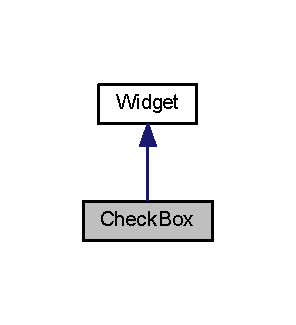
\includegraphics[width=142pt]{class_check_box__inherit__graph}
\end{center}
\end{figure}


Collaboration diagram for Check\+Box\+:
\nopagebreak
\begin{figure}[H]
\begin{center}
\leavevmode
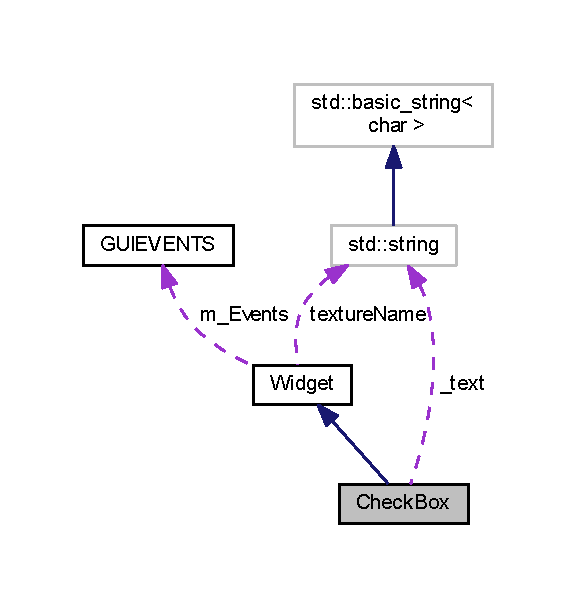
\includegraphics[width=277pt]{class_check_box__coll__graph}
\end{center}
\end{figure}
\subsection*{Public Member Functions}
\begin{DoxyCompactItemize}
\item 
{\bfseries Check\+Box} (float width, float height, int win\+Width, int win\+Height, std\+::string text)\hypertarget{class_check_box_a3d9390cf35471e93face354b98ff3001}{}\label{class_check_box_a3d9390cf35471e93face354b98ff3001}

\item 
void {\bfseries func} ()\hypertarget{class_check_box_a0b97039dee9e859cc9eb30d72e133a14}{}\label{class_check_box_a0b97039dee9e859cc9eb30d72e133a14}

\item 
const void {\bfseries Toggle} ()\hypertarget{class_check_box_a167a810d2ccddb3fec5a91520b6ae814}{}\label{class_check_box_a167a810d2ccddb3fec5a91520b6ae814}

\item 
glm\+::vec2 {\bfseries Calculate\+Resolution} (int w, int h, int ww, int wh)\hypertarget{class_check_box_ace23379528e35190569cf3e390d4632f}{}\label{class_check_box_ace23379528e35190569cf3e390d4632f}

\item 
void {\bfseries Render} (std\+::shared\+\_\+ptr$<$ \hyperlink{class_shader}{Shader} $>$ shader)\hypertarget{class_check_box_a52282c55293a750f37515b9bf1dc8aca}{}\label{class_check_box_a52282c55293a750f37515b9bf1dc8aca}

\item 
void {\bfseries Update} ()\hypertarget{class_check_box_a9ac8ab23419163e51aeb4bcf0a3b3114}{}\label{class_check_box_a9ac8ab23419163e51aeb4bcf0a3b3114}

\item 
void {\bfseries set\+Text} (std\+::string txt)\hypertarget{class_check_box_a9d2970b875aa42e476e656dfa0533e27}{}\label{class_check_box_a9d2970b875aa42e476e656dfa0533e27}

\item 
bool {\bfseries Checked} ()\hypertarget{class_check_box_a06cc98fa2259372559948cfe4656288c}{}\label{class_check_box_a06cc98fa2259372559948cfe4656288c}

\item 
void {\bfseries Check} ()\hypertarget{class_check_box_abab1504cfd126c3b13338db6171ae2d5}{}\label{class_check_box_abab1504cfd126c3b13338db6171ae2d5}

\item 
void {\bfseries Uncheck} ()\hypertarget{class_check_box_a79d07104121045ab7589e5bcee43c4c1}{}\label{class_check_box_a79d07104121045ab7589e5bcee43c4c1}

\end{DoxyCompactItemize}
\subsection*{Data Fields}
\begin{DoxyCompactItemize}
\item 
std\+::shared\+\_\+ptr$<$ \hyperlink{class_text}{Text} $>$ {\bfseries m\+\_\+\+Text\+Renderer\+Instance}\hypertarget{class_check_box_a89248e9f2d0168a99e480e2847f0b96b}{}\label{class_check_box_a89248e9f2d0168a99e480e2847f0b96b}

\end{DoxyCompactItemize}
\subsection*{Static Public Attributes}
\begin{DoxyCompactItemize}
\item 
static bool {\bfseries \+\_\+checked} = true\hypertarget{class_check_box_aaf46b8d854583decd71d82af3a84cd4c}{}\label{class_check_box_aaf46b8d854583decd71d82af3a84cd4c}

\end{DoxyCompactItemize}
\subsection*{Private Attributes}
\begin{DoxyCompactItemize}
\item 
std\+::function$<$ void()$>$ {\bfseries \+\_\+clickfunc}\hypertarget{class_check_box_af5af918560cc8733a4186a37af9d3ffc}{}\label{class_check_box_af5af918560cc8733a4186a37af9d3ffc}

\item 
std\+::shared\+\_\+ptr$<$ \hyperlink{classe_texture}{e\+Texture} $>$ {\bfseries \+\_\+checked\+Ico}\hypertarget{class_check_box_a57983f1421b9bdb7432fadb0d800dbfe}{}\label{class_check_box_a57983f1421b9bdb7432fadb0d800dbfe}

\item 
std\+::shared\+\_\+ptr$<$ \hyperlink{classe_texture}{e\+Texture} $>$ {\bfseries \+\_\+unchecked\+Ico}\hypertarget{class_check_box_ac2b7e23e182871b0b3c3f63b855dff38}{}\label{class_check_box_ac2b7e23e182871b0b3c3f63b855dff38}

\item 
glm\+::mat4 {\bfseries projection}\hypertarget{class_check_box_a9c7a7bbbdd801f86c54159dadf6761a9}{}\label{class_check_box_a9c7a7bbbdd801f86c54159dadf6761a9}

\item 
std\+::shared\+\_\+ptr$<$ \hyperlink{class_open_g_l_helpers_1_1_quad}{Open\+G\+L\+Helpers\+::\+Quad} $>$ {\bfseries m\+\_\+\+Quad}\hypertarget{class_check_box_a3eda2dffdfc108bcd052979c39ca061f}{}\label{class_check_box_a3eda2dffdfc108bcd052979c39ca061f}

\item 
std\+::string {\bfseries \+\_\+text}\hypertarget{class_check_box_adf8dfe43e7c761f7aa251c09d94536a6}{}\label{class_check_box_adf8dfe43e7c761f7aa251c09d94536a6}

\item 
std\+::shared\+\_\+ptr$<$ \hyperlink{class_shader}{Shader} $>$ {\bfseries m\+\_\+\+Check\+Box\+Shader}\hypertarget{class_check_box_a4f218da0aa68f868501e5a2c9194f4b2}{}\label{class_check_box_a4f218da0aa68f868501e5a2c9194f4b2}

\item 
float {\bfseries m\+\_\+\+Width}\hypertarget{class_check_box_a0ee5ae038afa76d504d657679e59b379}{}\label{class_check_box_a0ee5ae038afa76d504d657679e59b379}

\item 
float {\bfseries m\+\_\+\+Height}\hypertarget{class_check_box_ac89b5a9f404e10620e7451f22572c717}{}\label{class_check_box_ac89b5a9f404e10620e7451f22572c717}

\item 
float {\bfseries m\+\_\+win\+Width}\hypertarget{class_check_box_a532007421507bd6d4e7c71f1e788980f}{}\label{class_check_box_a532007421507bd6d4e7c71f1e788980f}

\item 
float {\bfseries m\+\_\+win\+Height}\hypertarget{class_check_box_a93bbceb8e7558727c7607b4b45f90305}{}\label{class_check_box_a93bbceb8e7558727c7607b4b45f90305}

\end{DoxyCompactItemize}
\subsection*{Additional Inherited Members}


\subsection{Detailed Description}


Definition at line 7 of file Check\+Box.\+h.


\hypertarget{class_component_1_1_cloth_component}{}\section{Component\+:\+:Cloth\+Component Class Reference}
\label{class_component_1_1_cloth_component}\index{Component\+::\+Cloth\+Component@{Component\+::\+Cloth\+Component}}


Inheritance diagram for Component\+:\+:Cloth\+Component\+:
\nopagebreak
\begin{figure}[H]
\begin{center}
\leavevmode
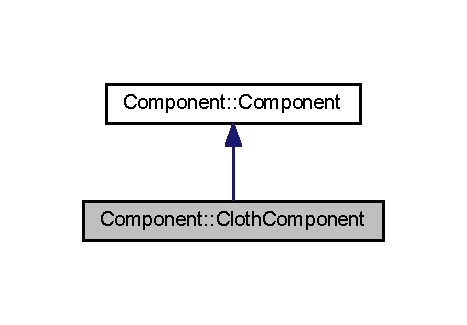
\includegraphics[width=224pt]{class_component_1_1_cloth_component__inherit__graph}
\end{center}
\end{figure}


Collaboration diagram for Component\+:\+:Cloth\+Component\+:
\nopagebreak
\begin{figure}[H]
\begin{center}
\leavevmode
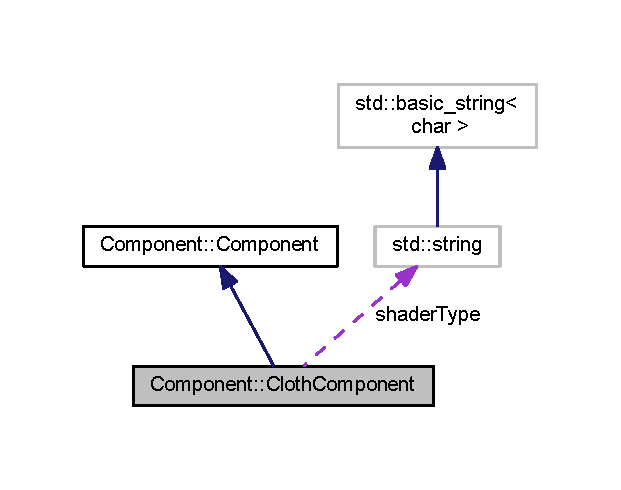
\includegraphics[width=298pt]{class_component_1_1_cloth_component__coll__graph}
\end{center}
\end{figure}
\subsection*{Public Member Functions}
\begin{DoxyCompactItemize}
\item 
{\bfseries Cloth\+Component} (std\+::shared\+\_\+ptr$<$ \hyperlink{class_camera}{Camera} $>$ \&in\+Pointer\+To\+Camera)\hypertarget{class_component_1_1_cloth_component_a9f1c6b25320d8c8ebb0a6db5a263954f}{}\label{class_component_1_1_cloth_component_a9f1c6b25320d8c8ebb0a6db5a263954f}

\item 
void {\bfseries Fill} (std\+::shared\+\_\+ptr$<$ \hyperlink{class_physics_1_1_physic_object}{Physics\+::\+Physic\+Object} $>$ Physic\+Body\+Pointer)\hypertarget{class_component_1_1_cloth_component_acb3b11f2564e72d5a0fb9c9baf61151f}{}\label{class_component_1_1_cloth_component_acb3b11f2564e72d5a0fb9c9baf61151f}

\item 
void {\bfseries Render} (std\+::shared\+\_\+ptr$<$ \hyperlink{class_resource_manager}{Resource\+Manager} $>$ rm, glm\+::vec3 pos)\hypertarget{class_component_1_1_cloth_component_a0c7111ca675b583947eec0db6325b879}{}\label{class_component_1_1_cloth_component_a0c7111ca675b583947eec0db6325b879}

\item 
virtual void {\bfseries Render\+Shadows} ()\hypertarget{class_component_1_1_cloth_component_acfc9cbff108906ad03de7fbd71a69a9a}{}\label{class_component_1_1_cloth_component_acfc9cbff108906ad03de7fbd71a69a9a}

\item 
void {\bfseries Update} (std\+::shared\+\_\+ptr$<$ \hyperlink{class_resource_manager}{Resource\+Manager} $>$ rm)\hypertarget{class_component_1_1_cloth_component_a8a65ac909f98708aa75775ab3621cafa}{}\label{class_component_1_1_cloth_component_a8a65ac909f98708aa75775ab3621cafa}

\item 
void {\bfseries set\+Shader} (std\+::string sh)\hypertarget{class_component_1_1_cloth_component_a1dd222f5b5b2dc28ff7dd5ed6821dd09}{}\label{class_component_1_1_cloth_component_a1dd222f5b5b2dc28ff7dd5ed6821dd09}

\item 
virtual void \hyperlink{class_component_1_1_cloth_component_a576710f899b875a602bf4768590a805e}{Fill} (bool, bool)
\item 
virtual void {\bfseries Fill} (float, std\+::shared\+\_\+ptr$<$ \hyperlink{class_physics_1_1_physic_object}{Physics\+::\+Physic\+Object} $>$ Physic\+Body\+Pointer)\hypertarget{class_component_1_1_cloth_component_ae8977bbe31adb63fced8a18d8dd1109c}{}\label{class_component_1_1_cloth_component_ae8977bbe31adb63fced8a18d8dd1109c}

\item 
virtual void {\bfseries Fill} (std\+::string path, std\+::shared\+\_\+ptr$<$ \hyperlink{class_resource_manager}{Resource\+Manager} $>$ \&rm, std\+::string shader)\hypertarget{class_component_1_1_cloth_component_a97e68ce0ee8a6f236f01969ced6b5140}{}\label{class_component_1_1_cloth_component_a97e68ce0ee8a6f236f01969ced6b5140}

\item 
void {\bfseries Render} ()\hypertarget{class_component_1_1_cloth_component_a18bbb264c9e8838068a7004258b7b3a8}{}\label{class_component_1_1_cloth_component_a18bbb264c9e8838068a7004258b7b3a8}

\item 
virtual void {\bfseries set\+Transparency} (bool x)\hypertarget{class_component_1_1_cloth_component_a0517b1f0aebec214588a8a8e7b5df8ea}{}\label{class_component_1_1_cloth_component_a0517b1f0aebec214588a8a8e7b5df8ea}

\end{DoxyCompactItemize}
\subsection*{Data Fields}
\begin{DoxyCompactItemize}
\item 
std\+::shared\+\_\+ptr$<$ \hyperlink{class_patch}{Patch} $>$ {\bfseries m\+Patch}\hypertarget{class_component_1_1_cloth_component_ae4cf4f211f24417a59b60ce4b2eb9e13}{}\label{class_component_1_1_cloth_component_ae4cf4f211f24417a59b60ce4b2eb9e13}

\item 
std\+::shared\+\_\+ptr$<$ \hyperlink{class_physics_1_1_physic_object}{Physics\+::\+Physic\+Object} $>$ {\bfseries Rigid\+Body\+Pointer} = nullptr\hypertarget{class_component_1_1_cloth_component_a35128603dac4023fa535f8b0d28e9332}{}\label{class_component_1_1_cloth_component_a35128603dac4023fa535f8b0d28e9332}

\item 
std\+::shared\+\_\+ptr$<$ \hyperlink{class_camera}{Camera} $>$ {\bfseries Pointer\+To\+Camera}\hypertarget{class_component_1_1_cloth_component_a81e871d180ce755dd3f0c73982b955ab}{}\label{class_component_1_1_cloth_component_a81e871d180ce755dd3f0c73982b955ab}

\item 
std\+::string {\bfseries shader\+Type}\hypertarget{class_component_1_1_cloth_component_ae35886ac9a93ab8547dbbc026190b716}{}\label{class_component_1_1_cloth_component_ae35886ac9a93ab8547dbbc026190b716}

\end{DoxyCompactItemize}


\subsection{Detailed Description}


Definition at line 297 of file Component.\+h.



\subsection{Member Function Documentation}
\index{Component\+::\+Cloth\+Component@{Component\+::\+Cloth\+Component}!Fill@{Fill}}
\index{Fill@{Fill}!Component\+::\+Cloth\+Component@{Component\+::\+Cloth\+Component}}
\subsubsection[{\texorpdfstring{Fill(bool, bool)}{Fill(bool, bool)}}]{\setlength{\rightskip}{0pt plus 5cm}virtual void Component\+::\+Cloth\+Component\+::\+Fill (
\begin{DoxyParamCaption}
\item[{bool}]{, }
\item[{bool}]{}
\end{DoxyParamCaption}
)\hspace{0.3cm}{\ttfamily [inline]}, {\ttfamily [virtual]}}\hypertarget{class_component_1_1_cloth_component_a576710f899b875a602bf4768590a805e}{}\label{class_component_1_1_cloth_component_a576710f899b875a602bf4768590a805e}
Functions declared for the sake of pure virtual function polymorphism, must not be used for production 

Implements \hyperlink{class_component_1_1_component}{Component\+::\+Component}.



Definition at line 345 of file Component.\+h.


\hypertarget{class_physics_1_1_cloth_physic_object}{}\section{Physics\+:\+:Cloth\+Physic\+Object Class Reference}
\label{class_physics_1_1_cloth_physic_object}\index{Physics\+::\+Cloth\+Physic\+Object@{Physics\+::\+Cloth\+Physic\+Object}}


Inheritance diagram for Physics\+:\+:Cloth\+Physic\+Object\+:
\nopagebreak
\begin{figure}[H]
\begin{center}
\leavevmode
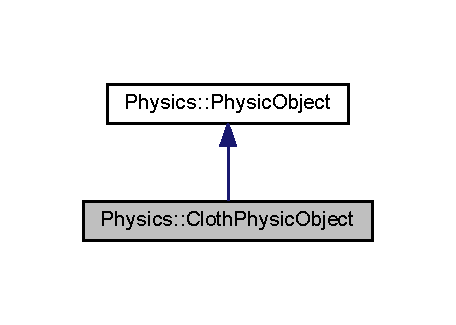
\includegraphics[width=219pt]{class_physics_1_1_cloth_physic_object__inherit__graph}
\end{center}
\end{figure}


Collaboration diagram for Physics\+:\+:Cloth\+Physic\+Object\+:
\nopagebreak
\begin{figure}[H]
\begin{center}
\leavevmode
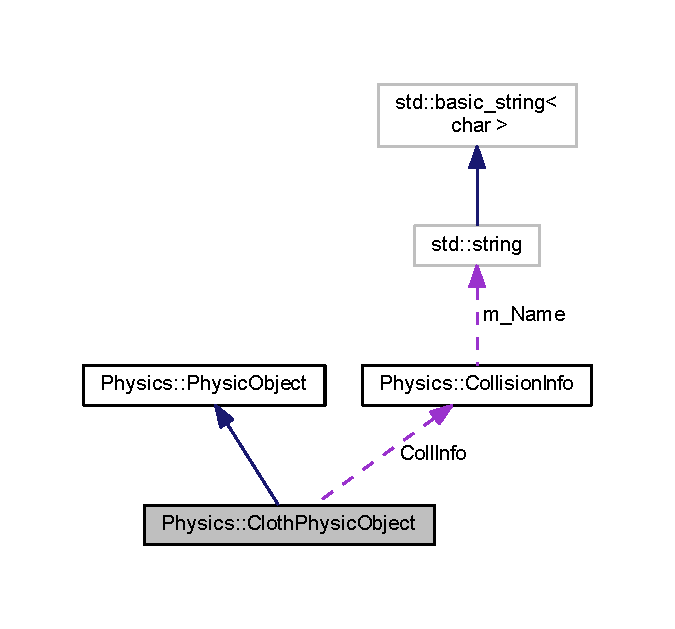
\includegraphics[width=324pt]{class_physics_1_1_cloth_physic_object__coll__graph}
\end{center}
\end{figure}
\subsection*{Public Member Functions}
\begin{DoxyCompactItemize}
\item 
virtual std\+::shared\+\_\+ptr$<$ bt\+Soft\+Body $>$ {\bfseries add\+Object} (std\+::shared\+\_\+ptr$<$ bt\+Soft\+Body\+World\+Info $>$ soft\+World\+Info, const glm\+::vec3 position, const bt\+Scalar s, const int numX, const int numY, const int fixed)\hypertarget{class_physics_1_1_cloth_physic_object_a78923cc91aae2576f71de7e1cfc1ef2b}{}\label{class_physics_1_1_cloth_physic_object_a78923cc91aae2576f71de7e1cfc1ef2b}

\item 
std\+::vector$<$ \hyperlink{struct_physics_1_1_physic_object_1_1t___cloth_vertex}{t\+\_\+\+Cloth\+Vertex} $>$ {\bfseries get\+Vertices} ()\hypertarget{class_physics_1_1_cloth_physic_object_a16c6ad9efd297a4f130bb4b91da4688f}{}\label{class_physics_1_1_cloth_physic_object_a16c6ad9efd297a4f130bb4b91da4688f}

\item 
float {\bfseries get\+Scale} ()\hypertarget{class_physics_1_1_cloth_physic_object_a3febd3bda1ef9e8e93e94cc492b08cb8}{}\label{class_physics_1_1_cloth_physic_object_a3febd3bda1ef9e8e93e94cc492b08cb8}

\item 
int {\bfseries get\+Width} ()\hypertarget{class_physics_1_1_cloth_physic_object_a1fe5c3095c7a9189f748c937f5a38035}{}\label{class_physics_1_1_cloth_physic_object_a1fe5c3095c7a9189f748c937f5a38035}

\item 
int {\bfseries get\+Height} ()\hypertarget{class_physics_1_1_cloth_physic_object_a18f471ffe72516280fdfbd94b9d86093}{}\label{class_physics_1_1_cloth_physic_object_a18f471ffe72516280fdfbd94b9d86093}

\item 
void {\bfseries set\+Wind} (bt\+Vector3 direction, float speed)\hypertarget{class_physics_1_1_cloth_physic_object_a7a62b2d5e8c4fb86b5eb8aebf40407d6}{}\label{class_physics_1_1_cloth_physic_object_a7a62b2d5e8c4fb86b5eb8aebf40407d6}

\item 
void {\bfseries setconstraint} (int x, int y)\hypertarget{class_physics_1_1_cloth_physic_object_a48b7fda6eb78e6d7fe01696553ef40be}{}\label{class_physics_1_1_cloth_physic_object_a48b7fda6eb78e6d7fe01696553ef40be}

\end{DoxyCompactItemize}
\subsection*{Data Fields}
\begin{DoxyCompactItemize}
\item 
std\+::shared\+\_\+ptr$<$ bt\+Soft\+Body $>$ {\bfseries m\+\_\+\+Body\+Cloth}\hypertarget{class_physics_1_1_cloth_physic_object_afc314d3b98724e0df6179b937595db22}{}\label{class_physics_1_1_cloth_physic_object_afc314d3b98724e0df6179b937595db22}

\item 
\hyperlink{class_physics_1_1_collision_info}{Collision\+Info} {\bfseries Coll\+Info}\hypertarget{class_physics_1_1_cloth_physic_object_a7fe0ba698cd4bcb4d82a25cb7e0e5aa2}{}\label{class_physics_1_1_cloth_physic_object_a7fe0ba698cd4bcb4d82a25cb7e0e5aa2}

\end{DoxyCompactItemize}
\subsection*{Private Attributes}
\begin{DoxyCompactItemize}
\item 
float {\bfseries m\+Scale}\hypertarget{class_physics_1_1_cloth_physic_object_ad9c5b1da6495f984ee0215d296677456}{}\label{class_physics_1_1_cloth_physic_object_ad9c5b1da6495f984ee0215d296677456}

\item 
int {\bfseries m\+Width}\hypertarget{class_physics_1_1_cloth_physic_object_aeab1e545b898d75f7f1b4b0bac94399a}{}\label{class_physics_1_1_cloth_physic_object_aeab1e545b898d75f7f1b4b0bac94399a}

\item 
int {\bfseries m\+Height}\hypertarget{class_physics_1_1_cloth_physic_object_a1e42276fd67a31e4cf892181382e9e64}{}\label{class_physics_1_1_cloth_physic_object_a1e42276fd67a31e4cf892181382e9e64}

\end{DoxyCompactItemize}


\subsection{Detailed Description}


Definition at line 10 of file Cloth\+Physic\+Object.\+h.


\hypertarget{class_physics_1_1_collision_info}{}\section{Physics\+:\+:Collision\+Info Class Reference}
\label{class_physics_1_1_collision_info}\index{Physics\+::\+Collision\+Info@{Physics\+::\+Collision\+Info}}


Collaboration diagram for Physics\+:\+:Collision\+Info\+:
\nopagebreak
\begin{figure}[H]
\begin{center}
\leavevmode
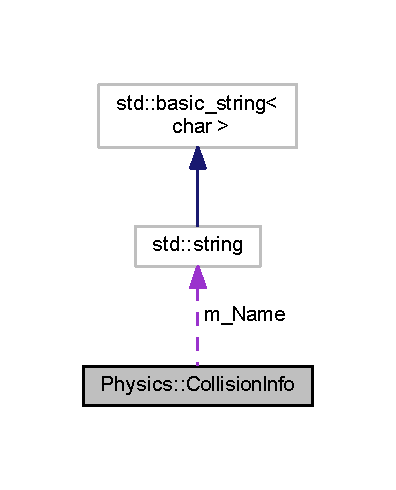
\includegraphics[width=190pt]{class_physics_1_1_collision_info__coll__graph}
\end{center}
\end{figure}
\subsection*{Public Member Functions}
\begin{DoxyCompactItemize}
\item 
std\+::string {\bfseries get\+Name} ()\hypertarget{class_physics_1_1_collision_info_a3194d945a48374db518166df543a54fc}{}\label{class_physics_1_1_collision_info_a3194d945a48374db518166df543a54fc}

\item 
void {\bfseries set\+Name} (std\+::string name)\hypertarget{class_physics_1_1_collision_info_aecf6846320be0f31c5d1c28f41dc4020}{}\label{class_physics_1_1_collision_info_aecf6846320be0f31c5d1c28f41dc4020}

\end{DoxyCompactItemize}
\subsection*{Private Attributes}
\begin{DoxyCompactItemize}
\item 
std\+::string {\bfseries m\+\_\+\+Name}\hypertarget{class_physics_1_1_collision_info_a800678029ef53f0deac515d85a72882b}{}\label{class_physics_1_1_collision_info_a800678029ef53f0deac515d85a72882b}

\end{DoxyCompactItemize}


\subsection{Detailed Description}


Definition at line 3 of file Collision\+Info.\+h.


\hypertarget{class_component_1_1_component}{}\section{Component\+:\+:Component Class Reference}
\label{class_component_1_1_component}\index{Component\+::\+Component@{Component\+::\+Component}}


Inheritance diagram for Component\+:\+:Component\+:
\nopagebreak
\begin{figure}[H]
\begin{center}
\leavevmode
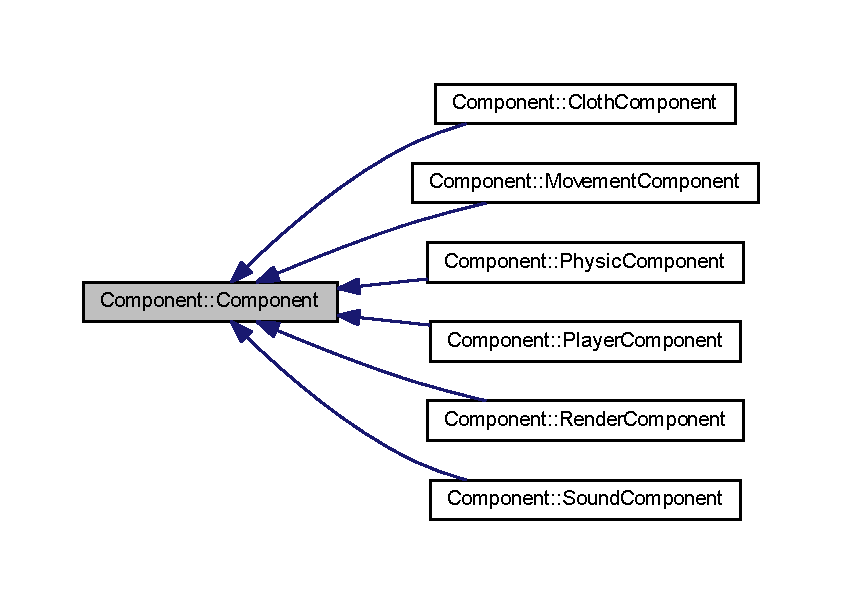
\includegraphics[width=350pt]{class_component_1_1_component__inherit__graph}
\end{center}
\end{figure}
\subsection*{Public Member Functions}
\begin{DoxyCompactItemize}
\item 
virtual void {\bfseries Fill} (bool Has\+Health, bool Has\+Gun)=0\hypertarget{class_component_1_1_component_a26353b4e284b63d84b929b86f6e9148b}{}\label{class_component_1_1_component_a26353b4e284b63d84b929b86f6e9148b}

\item 
virtual void {\bfseries Fill} (std\+::string path, std\+::shared\+\_\+ptr$<$ \hyperlink{class_resource_manager}{Resource\+Manager} $>$ \&rm, std\+::string shader)=0\hypertarget{class_component_1_1_component_a489a17c3dd7e1ee77959181533fa9d9a}{}\label{class_component_1_1_component_a489a17c3dd7e1ee77959181533fa9d9a}

\item 
virtual void {\bfseries Fill} (float mass, std\+::shared\+\_\+ptr$<$ \hyperlink{class_physics_1_1_physic_object}{Physics\+::\+Physic\+Object} $>$ Physic\+Body\+Pointer)=0\hypertarget{class_component_1_1_component_ae90e144d4395c5ab87bd0c6ba6b9bee7}{}\label{class_component_1_1_component_ae90e144d4395c5ab87bd0c6ba6b9bee7}

\item 
virtual void {\bfseries set\+User\+Pointer} (void $\ast$user\+Pointer)\hypertarget{class_component_1_1_component_a2dce4318453252ae4f290b06b810e31b}{}\label{class_component_1_1_component_a2dce4318453252ae4f290b06b810e31b}

\item 
virtual bt\+Transform {\bfseries get\+Transform} ()\hypertarget{class_component_1_1_component_a79cfa9368519bd1956cf52ee24636d47}{}\label{class_component_1_1_component_a79cfa9368519bd1956cf52ee24636d47}

\item 
virtual void {\bfseries set\+Transform} (bt\+Transform)\hypertarget{class_component_1_1_component_a077e191323027579fd41e1cc893a79e7}{}\label{class_component_1_1_component_a077e191323027579fd41e1cc893a79e7}

\item 
virtual void {\bfseries Update} (std\+::shared\+\_\+ptr$<$ \hyperlink{class_resource_manager}{Resource\+Manager} $>$ rm)=0\hypertarget{class_component_1_1_component_aa931d000ca1e0ba431213273755f622c}{}\label{class_component_1_1_component_aa931d000ca1e0ba431213273755f622c}

\item 
virtual void {\bfseries Render} (std\+::shared\+\_\+ptr$<$ \hyperlink{class_resource_manager}{Resource\+Manager} $>$ rm, glm\+::vec3)=0\hypertarget{class_component_1_1_component_ac485b3a9afb2f9dd593fa6b7714ad3cc}{}\label{class_component_1_1_component_ac485b3a9afb2f9dd593fa6b7714ad3cc}

\item 
virtual void {\bfseries Render\+Shadows} ()\hypertarget{class_component_1_1_component_a99c7072041c25a077cf4633669c1c984}{}\label{class_component_1_1_component_a99c7072041c25a077cf4633669c1c984}

\item 
virtual void {\bfseries set\+Transparency} (bool x)=0\hypertarget{class_component_1_1_component_af43987e6d8dadab7ef7aaee6629fa1e1}{}\label{class_component_1_1_component_af43987e6d8dadab7ef7aaee6629fa1e1}

\item 
void {\bfseries set\+Shader} (string sh)\hypertarget{class_component_1_1_component_a6a113766820370bb4cdc4129d2408a55}{}\label{class_component_1_1_component_a6a113766820370bb4cdc4129d2408a55}

\end{DoxyCompactItemize}
\subsection*{Data Fields}
\begin{DoxyCompactItemize}
\item 
C\+O\+M\+P\+O\+N\+E\+N\+T\+\_\+\+T\+Y\+PE {\bfseries Type}\hypertarget{class_component_1_1_component_af4dec3a51b9df784040cb5cd809d79fe}{}\label{class_component_1_1_component_af4dec3a51b9df784040cb5cd809d79fe}

\item 
bt\+Vector3 {\bfseries m\+\_\+\+Physics\+World\+Position}\hypertarget{class_component_1_1_component_a052f87b10a8099a7c5d1c177a13056df}{}\label{class_component_1_1_component_a052f87b10a8099a7c5d1c177a13056df}

\item 
bt\+Vector3 {\bfseries m\+\_\+\+Last\+Physics\+World\+Position}\hypertarget{class_component_1_1_component_a63bb972ef698fe609770899f252ccc53}{}\label{class_component_1_1_component_a63bb972ef698fe609770899f252ccc53}

\item 
bt\+Vector3 {\bfseries m\+\_\+\+Physics\+World\+Scale}\hypertarget{class_component_1_1_component_ad533f66011b8562f55af6ae4b56e374b}{}\label{class_component_1_1_component_ad533f66011b8562f55af6ae4b56e374b}

\item 
bt\+Quaternion {\bfseries m\+\_\+\+Physics\+World\+Rotation}\hypertarget{class_component_1_1_component_a7fefa7380768c1b96b67d65410cb0d90}{}\label{class_component_1_1_component_a7fefa7380768c1b96b67d65410cb0d90}

\item 
bt\+Quaternion {\bfseries m\+\_\+\+Last\+Physics\+World\+Rotation}\hypertarget{class_component_1_1_component_a4d549befaca3703195f7328791206770}{}\label{class_component_1_1_component_a4d549befaca3703195f7328791206770}

\item 
bool {\bfseries update\+If\+Out\+Of\+View} = true\hypertarget{class_component_1_1_component_a0a49f61f8df325e37d18972ef9efab7c}{}\label{class_component_1_1_component_a0a49f61f8df325e37d18972ef9efab7c}

\item 
bool {\bfseries is\+Transparent} = false\hypertarget{class_component_1_1_component_ac8579c1969e9b0f53366b5521dd9d89b}{}\label{class_component_1_1_component_ac8579c1969e9b0f53366b5521dd9d89b}

\item 
bool {\bfseries is\+Double\+Faced} = false\hypertarget{class_component_1_1_component_a9b9c018cd89f4f31d49232f4e47caf3e}{}\label{class_component_1_1_component_a9b9c018cd89f4f31d49232f4e47caf3e}

\end{DoxyCompactItemize}


\subsection{Detailed Description}


Definition at line 20 of file Component.\+h.


\hypertarget{class_console}{}\section{Console Class Reference}
\label{class_console}\index{Console@{Console}}


Inheritance diagram for Console\+:
\nopagebreak
\begin{figure}[H]
\begin{center}
\leavevmode
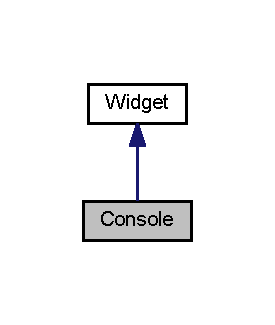
\includegraphics[width=132pt]{class_console__inherit__graph}
\end{center}
\end{figure}


Collaboration diagram for Console\+:
\nopagebreak
\begin{figure}[H]
\begin{center}
\leavevmode
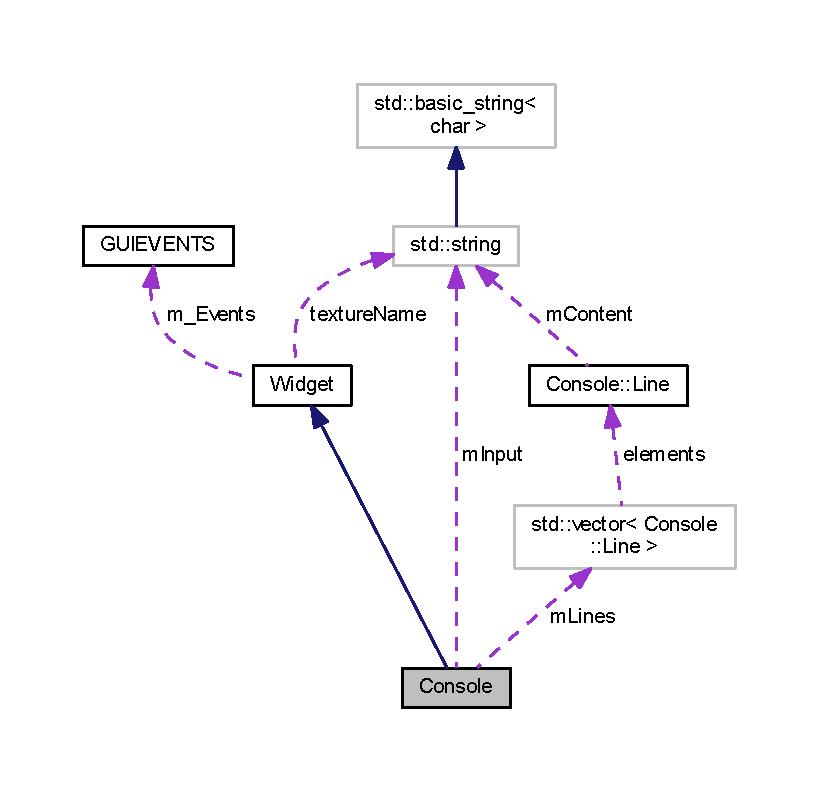
\includegraphics[width=350pt]{class_console__coll__graph}
\end{center}
\end{figure}
\subsection*{Data Structures}
\begin{DoxyCompactItemize}
\item 
class \hyperlink{class_console_1_1_line}{Line}
\end{DoxyCompactItemize}
\subsection*{Public Member Functions}
\begin{DoxyCompactItemize}
\item 
{\bfseries Console} (int w, int h, int fs, glm\+::vec4 c)\hypertarget{class_console_a15b54426649b02aabfc85d7abd800bc8}{}\label{class_console_a15b54426649b02aabfc85d7abd800bc8}

\item 
{\bfseries Render} ()\hypertarget{class_console_a885dd5651b11c34e24800fc574eb583f}{}\label{class_console_a885dd5651b11c34e24800fc574eb583f}

\item 
{\bfseries Toggle} ()\hypertarget{class_console_a3de86c2d04f5acdae65832c82b56b1ec}{}\label{class_console_a3de86c2d04f5acdae65832c82b56b1ec}

\item 
{\bfseries Add\+Command} ()\hypertarget{class_console_a10e1942df8cf654f330b808f4b88c7f8}{}\label{class_console_a10e1942df8cf654f330b808f4b88c7f8}

\item 
{\bfseries Execute\+Command} ()\hypertarget{class_console_a37444eaccb8b549612a0b0a6820e7a35}{}\label{class_console_a37444eaccb8b549612a0b0a6820e7a35}

\item 
bool {\bfseries is\+Showing} ()\hypertarget{class_console_af3841ee0141e0fef631021f68cc05cf3}{}\label{class_console_af3841ee0141e0fef631021f68cc05cf3}

\end{DoxyCompactItemize}
\subsection*{Private Member Functions}
\begin{DoxyCompactItemize}
\item 
void {\bfseries Render\+Frame} ()\hypertarget{class_console_a8e113a2a59fdb02689042b4e53cd5608}{}\label{class_console_a8e113a2a59fdb02689042b4e53cd5608}

\item 
void {\bfseries Render\+Scroll\+Bar} ()\hypertarget{class_console_a466e397fdf905d31903efda5835609e8}{}\label{class_console_a466e397fdf905d31903efda5835609e8}

\item 
void {\bfseries Render\+Text} ()\hypertarget{class_console_a6ae098af143802a2e3b6663568970c90}{}\label{class_console_a6ae098af143802a2e3b6663568970c90}

\item 
void {\bfseries Render\+Input\+Text} ()\hypertarget{class_console_a180276113ca697dad64eec27e6642960}{}\label{class_console_a180276113ca697dad64eec27e6642960}

\end{DoxyCompactItemize}
\subsection*{Private Attributes}
\begin{DoxyCompactItemize}
\item 
bool {\bfseries m\+Showing} = false\hypertarget{class_console_ae6dc828ddc2568d404c469680b8d3c0a}{}\label{class_console_ae6dc828ddc2568d404c469680b8d3c0a}

\item 
std\+::vector$<$ \hyperlink{class_console_1_1_line}{Line} $>$ {\bfseries m\+Lines}\hypertarget{class_console_a8bfc7c9805dd83446285616962985ae0}{}\label{class_console_a8bfc7c9805dd83446285616962985ae0}

\item 
std\+::string {\bfseries m\+Input}\hypertarget{class_console_a43845fdae982a31cfec85169d3b899b2}{}\label{class_console_a43845fdae982a31cfec85169d3b899b2}

\item 
int {\bfseries m\+Width}\hypertarget{class_console_a9914b424fbb8a60918de3166b8b151ae}{}\label{class_console_a9914b424fbb8a60918de3166b8b151ae}

\item 
int {\bfseries m\+Height}\hypertarget{class_console_a43e628863901714b6b825d103c20d9cb}{}\label{class_console_a43e628863901714b6b825d103c20d9cb}

\item 
int {\bfseries m\+Font\+Size}\hypertarget{class_console_a1dc666f022caaf0454de44494f63ec11}{}\label{class_console_a1dc666f022caaf0454de44494f63ec11}

\item 
glm\+::vec4 {\bfseries m\+Background\+Color}\hypertarget{class_console_ab28ca087e70d7835190053f919ea2f93}{}\label{class_console_ab28ca087e70d7835190053f919ea2f93}

\item 
glm\+::mat4 {\bfseries projection}\hypertarget{class_console_a6b6690bb5da085e17ab42f97778094fa}{}\label{class_console_a6b6690bb5da085e17ab42f97778094fa}

\item 
std\+::shared\+\_\+ptr$<$ \hyperlink{class_open_g_l_helpers_1_1_quad}{Open\+G\+L\+Helpers\+::\+Quad} $>$ {\bfseries m\+\_\+\+Quad}\hypertarget{class_console_a4a639bbd4321496f2c3e3a81fb50ff21}{}\label{class_console_a4a639bbd4321496f2c3e3a81fb50ff21}

\end{DoxyCompactItemize}
\subsection*{Additional Inherited Members}


\subsection{Detailed Description}


Definition at line 7 of file Console.\+h.


\hypertarget{class_container}{}\section{Container Class Reference}
\label{class_container}\index{Container@{Container}}


Collaboration diagram for Container\+:
\nopagebreak
\begin{figure}[H]
\begin{center}
\leavevmode
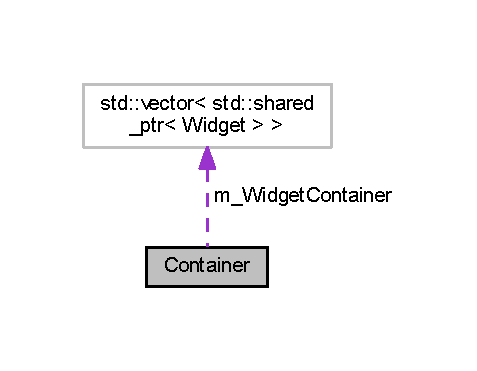
\includegraphics[width=229pt]{class_container__coll__graph}
\end{center}
\end{figure}
\subsection*{Public Member Functions}
\begin{DoxyCompactItemize}
\item 
bool {\bfseries add\+Widget} (std\+::shared\+\_\+ptr$<$ \hyperlink{class_widget}{Widget} $>$ widget)\hypertarget{class_container_afb008983dab9b54b9281954acce7a769}{}\label{class_container_afb008983dab9b54b9281954acce7a769}

\item 
void {\bfseries Render} (std\+::shared\+\_\+ptr$<$ \hyperlink{class_shader}{Shader} $>$ shader)\hypertarget{class_container_a3f42908e326e7cd5e02922bcdafe126c}{}\label{class_container_a3f42908e326e7cd5e02922bcdafe126c}

\item 
void {\bfseries Analize\+Events} (\hyperlink{struct_g_u_i_e_v_e_n_t_s}{G\+U\+I\+E\+V\+E\+N\+TS} Events)\hypertarget{class_container_aa80ad9b67044647b6891443b94098beb}{}\label{class_container_aa80ad9b67044647b6891443b94098beb}

\end{DoxyCompactItemize}
\subsection*{Private Attributes}
\begin{DoxyCompactItemize}
\item 
std\+::vector$<$ std\+::shared\+\_\+ptr$<$ \hyperlink{class_widget}{Widget} $>$ $>$ {\bfseries m\+\_\+\+Widget\+Container}\hypertarget{class_container_ae071597fef1204072f500f7384b5ae47}{}\label{class_container_ae071597fef1204072f500f7384b5ae47}

\end{DoxyCompactItemize}


\subsection{Detailed Description}


Definition at line 4 of file Container.\+h.


\hypertarget{class_c_p_u_i_d}{}\section{C\+P\+U\+ID Class Reference}
\label{class_c_p_u_i_d}\index{C\+P\+U\+ID@{C\+P\+U\+ID}}
\subsection*{Public Member Functions}
\begin{DoxyCompactItemize}
\item 
{\bfseries C\+P\+U\+ID} (unsigned i)\hypertarget{class_c_p_u_i_d_a18c6241f3f65fce5f97d0cf89e75f367}{}\label{class_c_p_u_i_d_a18c6241f3f65fce5f97d0cf89e75f367}

\item 
const uint32\+\_\+t \& {\bfseries E\+AX} () const \hypertarget{class_c_p_u_i_d_aa6601284e70a0916d9c469480966cbd7}{}\label{class_c_p_u_i_d_aa6601284e70a0916d9c469480966cbd7}

\item 
const uint32\+\_\+t \& {\bfseries E\+BX} () const \hypertarget{class_c_p_u_i_d_a00be36d9d083febb307c3ae6e38feac7}{}\label{class_c_p_u_i_d_a00be36d9d083febb307c3ae6e38feac7}

\item 
const uint32\+\_\+t \& {\bfseries E\+CX} () const \hypertarget{class_c_p_u_i_d_a33f163100a8f91ad81cbe56e2bd506d0}{}\label{class_c_p_u_i_d_a33f163100a8f91ad81cbe56e2bd506d0}

\item 
const uint32\+\_\+t \& {\bfseries E\+DX} () const \hypertarget{class_c_p_u_i_d_ab17d7f6f0a18ff5e5e8ecf1a22e25d89}{}\label{class_c_p_u_i_d_ab17d7f6f0a18ff5e5e8ecf1a22e25d89}

\item 
std\+::string {\bfseries get\+C\+P\+U\+Vendor} ()\hypertarget{class_c_p_u_i_d_ad9b9499f6e31a04536ee1242868faa17}{}\label{class_c_p_u_i_d_ad9b9499f6e31a04536ee1242868faa17}

\item 
bool {\bfseries get\+Endianes} ()\hypertarget{class_c_p_u_i_d_af31074460d6eae80a9920b58cbb19853}{}\label{class_c_p_u_i_d_af31074460d6eae80a9920b58cbb19853}

\item 
unsigned {\bfseries get\+Number\+Of\+Threads} ()\hypertarget{class_c_p_u_i_d_a4785c8f6b530e3b4b0fbe042dcc91140}{}\label{class_c_p_u_i_d_a4785c8f6b530e3b4b0fbe042dcc91140}

\item 
void {\bfseries print\+Hardware\+Information} ()\hypertarget{class_c_p_u_i_d_ab1fa95dd39b3e393ac82099fe6354c5c}{}\label{class_c_p_u_i_d_ab1fa95dd39b3e393ac82099fe6354c5c}

\end{DoxyCompactItemize}
\subsection*{Private Attributes}
\begin{DoxyCompactItemize}
\item 
uint32\+\_\+t {\bfseries regs} \mbox{[}4\mbox{]}\hypertarget{class_c_p_u_i_d_a3f833ee5ea4135a5604c563d25aaa7e2}{}\label{class_c_p_u_i_d_a3f833ee5ea4135a5604c563d25aaa7e2}

\end{DoxyCompactItemize}


\subsection{Detailed Description}


Definition at line 10 of file C\+P\+U\+I\+D.\+h.


\hypertarget{class_c_quake3_b_s_p}{}\section{C\+Quake3\+B\+SP Class Reference}
\label{class_c_quake3_b_s_p}\index{C\+Quake3\+B\+SP@{C\+Quake3\+B\+SP}}


Collaboration diagram for C\+Quake3\+B\+SP\+:
\nopagebreak
\begin{figure}[H]
\begin{center}
\leavevmode
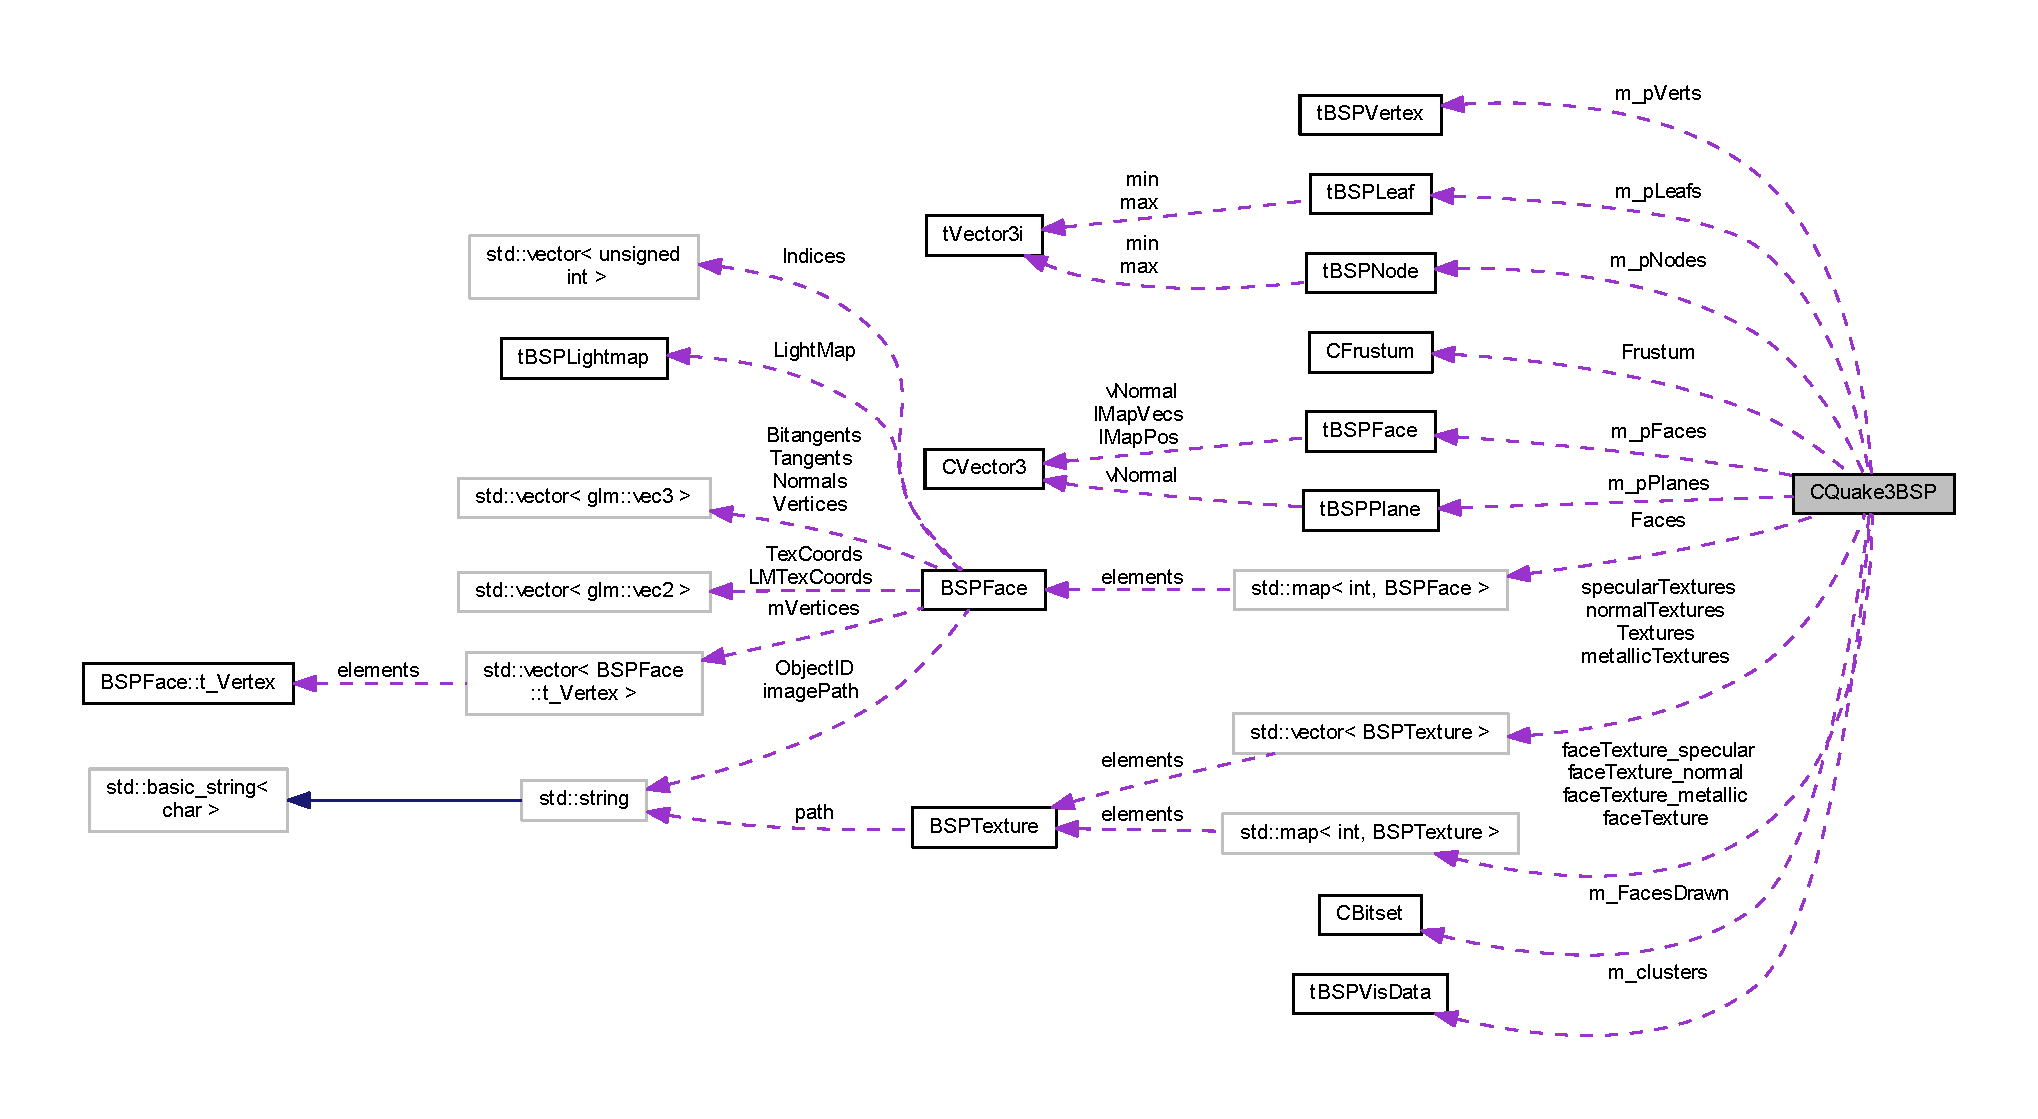
\includegraphics[width=350pt]{class_c_quake3_b_s_p__coll__graph}
\end{center}
\end{figure}
\subsection*{Public Member Functions}
\begin{DoxyCompactItemize}
\item 
{\bfseries C\+Quake3\+B\+SP} (std\+::shared\+\_\+ptr$<$ \hyperlink{class_resource_manager}{Resource\+Manager} $>$)\hypertarget{class_c_quake3_b_s_p_ade103aa4e41c95c7d8d96e4dc8fa5b6e}{}\label{class_c_quake3_b_s_p_ade103aa4e41c95c7d8d96e4dc8fa5b6e}

\item 
bool \hyperlink{class_c_quake3_b_s_p_a63f458d8e84eb5a4f0432460c849ba75}{Load\+B\+SP} (const char $\ast$str\+File\+Name)
\item 
void \hyperlink{class_c_quake3_b_s_p_adb06c36ee906c9c4db1d16c1642c3aa2}{Render\+Level} (glm\+::vec3 v\+Pos, G\+Luint shader, bool Shadow)
\item 
void {\bfseries Destroy} ()\hypertarget{class_c_quake3_b_s_p_aa61b5bb7e4dfe39ce88a023f438cbe77}{}\label{class_c_quake3_b_s_p_aa61b5bb7e4dfe39ce88a023f438cbe77}

\end{DoxyCompactItemize}
\subsection*{Data Fields}
\begin{DoxyCompactItemize}
\item 
\hyperlink{class_c_frustum}{C\+Frustum} {\bfseries Frustum}\hypertarget{class_c_quake3_b_s_p_ab3535b50e4d79b894aad24c1960ad718}{}\label{class_c_quake3_b_s_p_ab3535b50e4d79b894aad24c1960ad718}

\end{DoxyCompactItemize}
\subsection*{Private Member Functions}
\begin{DoxyCompactItemize}
\item 
void {\bfseries Find\+Texture\+Extension} (char $\ast$str\+File\+Name)\hypertarget{class_c_quake3_b_s_p_a81aaf95313a6b9d59ea088042870bbca}{}\label{class_c_quake3_b_s_p_a81aaf95313a6b9d59ea088042870bbca}

\item 
void {\bfseries Render\+Face} (int face\+Index, G\+Luint shader, bool)\hypertarget{class_c_quake3_b_s_p_ad1775eac850f6057170f7009e9fba55d}{}\label{class_c_quake3_b_s_p_ad1775eac850f6057170f7009e9fba55d}

\item 
int {\bfseries Is\+Cluster\+Visible} (int current, int test)\hypertarget{class_c_quake3_b_s_p_a8e69e5687f268bc56bff5faf341d597c}{}\label{class_c_quake3_b_s_p_a8e69e5687f268bc56bff5faf341d597c}

\item 
int \hyperlink{class_c_quake3_b_s_p_a82ab93b599790d05ebf7039aa811cee5}{Find\+Leaf} (glm\+::vec3 v\+Pos)
\end{DoxyCompactItemize}
\subsection*{Private Attributes}
\begin{DoxyCompactItemize}
\item 
int {\bfseries m\+\_\+num\+Of\+Verts}\hypertarget{class_c_quake3_b_s_p_a8ae3f4273747ba0c3895a8d633ce2454}{}\label{class_c_quake3_b_s_p_a8ae3f4273747ba0c3895a8d633ce2454}

\item 
int {\bfseries m\+\_\+num\+Of\+Faces}\hypertarget{class_c_quake3_b_s_p_af5a83586ec3fef2ccd908f35d5a7ed4f}{}\label{class_c_quake3_b_s_p_af5a83586ec3fef2ccd908f35d5a7ed4f}

\item 
int {\bfseries m\+\_\+num\+Of\+Indices}\hypertarget{class_c_quake3_b_s_p_aae87231445fa33c309d01df02fafb4a9}{}\label{class_c_quake3_b_s_p_aae87231445fa33c309d01df02fafb4a9}

\item 
int {\bfseries m\+\_\+num\+Of\+Textures}\hypertarget{class_c_quake3_b_s_p_a993aca8bb89197243d7b10c69bc25a62}{}\label{class_c_quake3_b_s_p_a993aca8bb89197243d7b10c69bc25a62}

\item 
int {\bfseries m\+\_\+num\+Of\+Lightmaps}\hypertarget{class_c_quake3_b_s_p_afe912e0cd3b2b30eb49637e0ce4c2538}{}\label{class_c_quake3_b_s_p_afe912e0cd3b2b30eb49637e0ce4c2538}

\item 
int {\bfseries m\+\_\+num\+Of\+Nodes}\hypertarget{class_c_quake3_b_s_p_ab36e7f94bcfa3bb51daa37ced0aa2b58}{}\label{class_c_quake3_b_s_p_ab36e7f94bcfa3bb51daa37ced0aa2b58}

\item 
int {\bfseries m\+\_\+num\+Of\+Leafs}\hypertarget{class_c_quake3_b_s_p_abd7ba3b4d1c3bfd69e501a37cd5fe8fc}{}\label{class_c_quake3_b_s_p_abd7ba3b4d1c3bfd69e501a37cd5fe8fc}

\item 
int {\bfseries m\+\_\+num\+Of\+Leaf\+Faces}\hypertarget{class_c_quake3_b_s_p_ad8f12c640f5a931b3ef55f06b7056611}{}\label{class_c_quake3_b_s_p_ad8f12c640f5a931b3ef55f06b7056611}

\item 
int {\bfseries m\+\_\+num\+Of\+Planes}\hypertarget{class_c_quake3_b_s_p_a65587e5eb28496e59f049cad7f5f7c1b}{}\label{class_c_quake3_b_s_p_a65587e5eb28496e59f049cad7f5f7c1b}

\item 
int $\ast$ {\bfseries m\+\_\+p\+Indices}\hypertarget{class_c_quake3_b_s_p_a58ccdf0e96cc03e690859e2205fbbe02}{}\label{class_c_quake3_b_s_p_a58ccdf0e96cc03e690859e2205fbbe02}

\item 
\hyperlink{structt_b_s_p_vertex}{t\+B\+S\+P\+Vertex} $\ast$ {\bfseries m\+\_\+p\+Verts}\hypertarget{class_c_quake3_b_s_p_aa8b1307c8cadac3fbdaa2d2090689b30}{}\label{class_c_quake3_b_s_p_aa8b1307c8cadac3fbdaa2d2090689b30}

\item 
\hyperlink{structt_b_s_p_face}{t\+B\+S\+P\+Face} $\ast$ {\bfseries m\+\_\+p\+Faces}\hypertarget{class_c_quake3_b_s_p_ac341d879b0d52ed6036be45b117b0800}{}\label{class_c_quake3_b_s_p_ac341d879b0d52ed6036be45b117b0800}

\item 
\hyperlink{structt_b_s_p_node}{t\+B\+S\+P\+Node} $\ast$ {\bfseries m\+\_\+p\+Nodes}\hypertarget{class_c_quake3_b_s_p_a61af50f0545e0e9f17b30ba29a6d3012}{}\label{class_c_quake3_b_s_p_a61af50f0545e0e9f17b30ba29a6d3012}

\item 
\hyperlink{structt_b_s_p_leaf}{t\+B\+S\+P\+Leaf} $\ast$ {\bfseries m\+\_\+p\+Leafs}\hypertarget{class_c_quake3_b_s_p_ae45c76a84f9a10fd63a784a555018664}{}\label{class_c_quake3_b_s_p_ae45c76a84f9a10fd63a784a555018664}

\item 
\hyperlink{structt_b_s_p_plane}{t\+B\+S\+P\+Plane} $\ast$ {\bfseries m\+\_\+p\+Planes}\hypertarget{class_c_quake3_b_s_p_a3dcce071fe25a7e261b625ca136fbf6e}{}\label{class_c_quake3_b_s_p_a3dcce071fe25a7e261b625ca136fbf6e}

\item 
int $\ast$ {\bfseries m\+\_\+p\+Leaf\+Faces}\hypertarget{class_c_quake3_b_s_p_ae9d2411614785d4dcb304f6a17ffd2d6}{}\label{class_c_quake3_b_s_p_ae9d2411614785d4dcb304f6a17ffd2d6}

\item 
\hyperlink{structt_b_s_p_vis_data}{t\+B\+S\+P\+Vis\+Data} {\bfseries m\+\_\+clusters}\hypertarget{class_c_quake3_b_s_p_af579c8cdab13d65d04b8fe21da37dde6}{}\label{class_c_quake3_b_s_p_af579c8cdab13d65d04b8fe21da37dde6}

\item 
unsigned int {\bfseries m\+\_\+textures} \mbox{[}M\+A\+X\+\_\+\+T\+E\+X\+T\+U\+R\+ES\mbox{]}\hypertarget{class_c_quake3_b_s_p_ad39344a841f60c33fbad46c354cc1c04}{}\label{class_c_quake3_b_s_p_ad39344a841f60c33fbad46c354cc1c04}

\item 
\hyperlink{class_c_bitset}{C\+Bitset} {\bfseries m\+\_\+\+Faces\+Drawn}\hypertarget{class_c_quake3_b_s_p_a91c15f2d32d87985fdd6ea874e1f9707}{}\label{class_c_quake3_b_s_p_a91c15f2d32d87985fdd6ea874e1f9707}

\item 
std\+::map$<$ int, \hyperlink{class_b_s_p_face}{B\+S\+P\+Face} $>$ {\bfseries Faces}\hypertarget{class_c_quake3_b_s_p_a3abb90858963d1d795b5e5e33a152f92}{}\label{class_c_quake3_b_s_p_a3abb90858963d1d795b5e5e33a152f92}

\item 
std\+::vector$<$ \hyperlink{struct_b_s_p_texture}{B\+S\+P\+Texture} $>$ {\bfseries Textures}\hypertarget{class_c_quake3_b_s_p_ae0e924f8e1ec9d4e911e4d9bdce5a1dd}{}\label{class_c_quake3_b_s_p_ae0e924f8e1ec9d4e911e4d9bdce5a1dd}

\item 
std\+::vector$<$ \hyperlink{struct_b_s_p_texture}{B\+S\+P\+Texture} $>$ {\bfseries normal\+Textures}\hypertarget{class_c_quake3_b_s_p_a83c453f608fa2799750da3705309aba4}{}\label{class_c_quake3_b_s_p_a83c453f608fa2799750da3705309aba4}

\item 
std\+::vector$<$ \hyperlink{struct_b_s_p_texture}{B\+S\+P\+Texture} $>$ {\bfseries specular\+Textures}\hypertarget{class_c_quake3_b_s_p_a38864b6aeb49897e7e836ca3ca306913}{}\label{class_c_quake3_b_s_p_a38864b6aeb49897e7e836ca3ca306913}

\item 
std\+::vector$<$ \hyperlink{struct_b_s_p_texture}{B\+S\+P\+Texture} $>$ {\bfseries metallic\+Textures}\hypertarget{class_c_quake3_b_s_p_acb1e64479b9861f90d79d4e84c10f725}{}\label{class_c_quake3_b_s_p_acb1e64479b9861f90d79d4e84c10f725}

\item 
std\+::map$<$ int, \hyperlink{struct_b_s_p_texture}{B\+S\+P\+Texture} $>$ {\bfseries face\+Texture}\hypertarget{class_c_quake3_b_s_p_adf1d74f1aa4e4bef4d0f467a6eaf863f}{}\label{class_c_quake3_b_s_p_adf1d74f1aa4e4bef4d0f467a6eaf863f}

\item 
std\+::map$<$ int, \hyperlink{struct_b_s_p_texture}{B\+S\+P\+Texture} $>$ {\bfseries face\+Texture\+\_\+normal}\hypertarget{class_c_quake3_b_s_p_a93aa930777a9843962fe40811ae0c050}{}\label{class_c_quake3_b_s_p_a93aa930777a9843962fe40811ae0c050}

\item 
std\+::map$<$ int, \hyperlink{struct_b_s_p_texture}{B\+S\+P\+Texture} $>$ {\bfseries face\+Texture\+\_\+specular}\hypertarget{class_c_quake3_b_s_p_a1ccd0446e9df6e7e6ec5f8f5c7ef551b}{}\label{class_c_quake3_b_s_p_a1ccd0446e9df6e7e6ec5f8f5c7ef551b}

\item 
std\+::map$<$ int, \hyperlink{struct_b_s_p_texture}{B\+S\+P\+Texture} $>$ {\bfseries face\+Texture\+\_\+metallic}\hypertarget{class_c_quake3_b_s_p_aef04d61cd502bb4ff5b7baadaf1e2425}{}\label{class_c_quake3_b_s_p_aef04d61cd502bb4ff5b7baadaf1e2425}

\item 
std\+::shared\+\_\+ptr$<$ \hyperlink{class_resource_manager}{Resource\+Manager} $>$ {\bfseries resm}\hypertarget{class_c_quake3_b_s_p_a31582b175495cba4efe12a246e2c0556}{}\label{class_c_quake3_b_s_p_a31582b175495cba4efe12a246e2c0556}

\item 
bool {\bfseries lightmap}\hypertarget{class_c_quake3_b_s_p_aef6f1b37165988413a0b2e6c94cc8318}{}\label{class_c_quake3_b_s_p_aef6f1b37165988413a0b2e6c94cc8318}

\item 
bool {\bfseries color}\hypertarget{class_c_quake3_b_s_p_aab755fee798e3a61e5ea781565fd1d89}{}\label{class_c_quake3_b_s_p_aab755fee798e3a61e5ea781565fd1d89}

\item 
int {\bfseries face\+Count}\hypertarget{class_c_quake3_b_s_p_a7153ffaf217255a815b837862a9d2f9a}{}\label{class_c_quake3_b_s_p_a7153ffaf217255a815b837862a9d2f9a}

\item 
G\+Luint {\bfseries Normal\+Texture\+ID}\hypertarget{class_c_quake3_b_s_p_a0daebdd8ca8923f8a0aa6d35e962a7b3}{}\label{class_c_quake3_b_s_p_a0daebdd8ca8923f8a0aa6d35e962a7b3}

\end{DoxyCompactItemize}


\subsection{Detailed Description}


Definition at line 225 of file B\+S\+P.\+h.



\subsection{Member Function Documentation}
\index{C\+Quake3\+B\+SP@{C\+Quake3\+B\+SP}!Find\+Leaf@{Find\+Leaf}}
\index{Find\+Leaf@{Find\+Leaf}!C\+Quake3\+B\+SP@{C\+Quake3\+B\+SP}}
\subsubsection[{\texorpdfstring{Find\+Leaf(glm\+::vec3 v\+Pos)}{FindLeaf(glm::vec3 vPos)}}]{\setlength{\rightskip}{0pt plus 5cm}int C\+Quake3\+B\+S\+P\+::\+Find\+Leaf (
\begin{DoxyParamCaption}
\item[{glm\+::vec3}]{v\+Pos}
\end{DoxyParamCaption}
)\hspace{0.3cm}{\ttfamily [private]}}\hypertarget{class_c_quake3_b_s_p_a82ab93b599790d05ebf7039aa811cee5}{}\label{class_c_quake3_b_s_p_a82ab93b599790d05ebf7039aa811cee5}
Binary operation 

Definition at line 351 of file B\+S\+P.\+cpp.

\index{C\+Quake3\+B\+SP@{C\+Quake3\+B\+SP}!Load\+B\+SP@{Load\+B\+SP}}
\index{Load\+B\+SP@{Load\+B\+SP}!C\+Quake3\+B\+SP@{C\+Quake3\+B\+SP}}
\subsubsection[{\texorpdfstring{Load\+B\+S\+P(const char $\ast$str\+File\+Name)}{LoadBSP(const char *strFileName)}}]{\setlength{\rightskip}{0pt plus 5cm}bool C\+Quake3\+B\+S\+P\+::\+Load\+B\+SP (
\begin{DoxyParamCaption}
\item[{const char $\ast$}]{str\+File\+Name}
\end{DoxyParamCaption}
)}\hypertarget{class_c_quake3_b_s_p_a63f458d8e84eb5a4f0432460c849ba75}{}\label{class_c_quake3_b_s_p_a63f458d8e84eb5a4f0432460c849ba75}
cout $<$$<$ \char`\"{}\+Number of lightmaps \+: \char`\"{} $<$$<$ lumps\mbox{[}k\+Lightmaps\mbox{]}.length / sizeof(t\+B\+S\+P\+Lightmap) $<$$<$ endl;

Used to Smooth the normals of the whole B\+SP map 

Definition at line 33 of file B\+S\+P.\+cpp.



Here is the call graph for this function\+:
\nopagebreak
\begin{figure}[H]
\begin{center}
\leavevmode
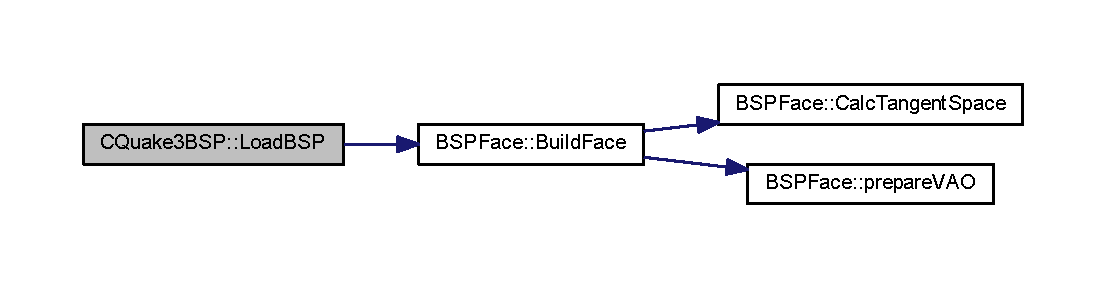
\includegraphics[width=350pt]{class_c_quake3_b_s_p_a63f458d8e84eb5a4f0432460c849ba75_cgraph}
\end{center}
\end{figure}


\index{C\+Quake3\+B\+SP@{C\+Quake3\+B\+SP}!Render\+Level@{Render\+Level}}
\index{Render\+Level@{Render\+Level}!C\+Quake3\+B\+SP@{C\+Quake3\+B\+SP}}
\subsubsection[{\texorpdfstring{Render\+Level(glm\+::vec3 v\+Pos, G\+Luint shader, bool Shadow)}{RenderLevel(glm::vec3 vPos, GLuint shader, bool Shadow)}}]{\setlength{\rightskip}{0pt plus 5cm}void C\+Quake3\+B\+S\+P\+::\+Render\+Level (
\begin{DoxyParamCaption}
\item[{glm\+::vec3}]{v\+Pos, }
\item[{G\+Luint}]{shader, }
\item[{bool}]{Shadow}
\end{DoxyParamCaption}
)}\hypertarget{class_c_quake3_b_s_p_adb06c36ee906c9c4db1d16c1642c3aa2}{}\label{class_c_quake3_b_s_p_adb06c36ee906c9c4db1d16c1642c3aa2}
glfw\+Set\+Window\+Title(window, (\char`\"{}\+Faces Drawn\+: \char`\"{} + to\+\_\+string(g\+\_\+\+Visible\+Faces)).c\+\_\+str()); 

Definition at line 407 of file B\+S\+P.\+cpp.


\hypertarget{class_cube_map}{}\section{Cube\+Map Class Reference}
\label{class_cube_map}\index{Cube\+Map@{Cube\+Map}}


Inheritance diagram for Cube\+Map\+:
\nopagebreak
\begin{figure}[H]
\begin{center}
\leavevmode
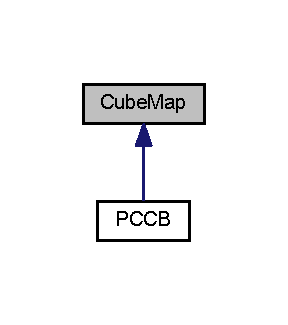
\includegraphics[width=138pt]{class_cube_map__inherit__graph}
\end{center}
\end{figure}


Collaboration diagram for Cube\+Map\+:
\nopagebreak
\begin{figure}[H]
\begin{center}
\leavevmode
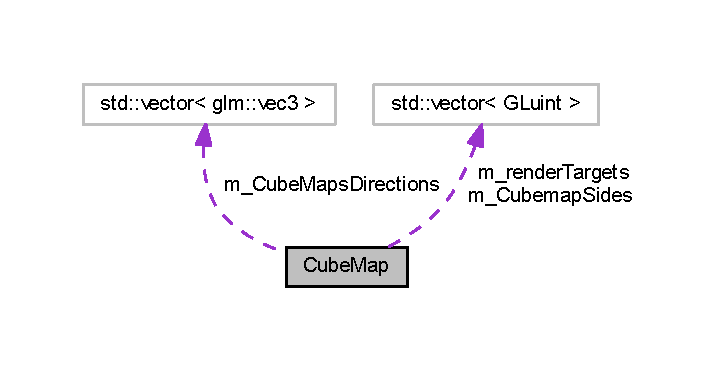
\includegraphics[width=345pt]{class_cube_map__coll__graph}
\end{center}
\end{figure}
\subsection*{Public Member Functions}
\begin{DoxyCompactItemize}
\item 
{\bfseries Cube\+Map} (int ID, glm\+::vec3 Pos)\hypertarget{class_cube_map_a83b70c2d6512569a18a2635c80ce016f}{}\label{class_cube_map_a83b70c2d6512569a18a2635c80ce016f}

\item 
{\bfseries Cube\+Map} (std\+::vector$<$ std\+::string $>$ paths, int ID, glm\+::vec3 Pos)\hypertarget{class_cube_map_a378d9efce6a735333fa729b41139311c}{}\label{class_cube_map_a378d9efce6a735333fa729b41139311c}

\item 
virtual void {\bfseries Capture\+Environment} (int index)\hypertarget{class_cube_map_a0a61a5ed08518ba002f23fbc5d8e9d05}{}\label{class_cube_map_a0a61a5ed08518ba002f23fbc5d8e9d05}

\item 
void {\bfseries end\+Capturing\+Environment} ()\hypertarget{class_cube_map_a61c5c70fffa991f6ed4f89a0dbb22e0a}{}\label{class_cube_map_a61c5c70fffa991f6ed4f89a0dbb22e0a}

\item 
void {\bfseries gen\+Frame\+Buffer} ()\hypertarget{class_cube_map_a37dd1b5096863f271a82a73774890d7c}{}\label{class_cube_map_a37dd1b5096863f271a82a73774890d7c}

\item 
void {\bfseries gen\+Ambient\+Convolution} ()\hypertarget{class_cube_map_a0797ebc5b6ba76861e75f0430fc1e905}{}\label{class_cube_map_a0797ebc5b6ba76861e75f0430fc1e905}

\item 
glm\+::mat4 {\bfseries get\+View\+Matrixby\+Index} (int index)\hypertarget{class_cube_map_a1f30c27f1f2d8498e4ac7a56f35d458e}{}\label{class_cube_map_a1f30c27f1f2d8498e4ac7a56f35d458e}

\item 
glm\+::mat4 {\bfseries get\+Projection\+Matrix} ()\hypertarget{class_cube_map_ac48b4b3164ffe920b8e9b0399c11f540}{}\label{class_cube_map_ac48b4b3164ffe920b8e9b0399c11f540}

\item 
virtual glm\+::vec3 {\bfseries get\+Position} ()\hypertarget{class_cube_map_a1fd3790fa6d80720250fc0359e692a2e}{}\label{class_cube_map_a1fd3790fa6d80720250fc0359e692a2e}

\item 
virtual G\+Luint {\bfseries get\+Texture\+ID} ()\hypertarget{class_cube_map_ae53c8617abedefbac800926e0e1996bc}{}\label{class_cube_map_ae53c8617abedefbac800926e0e1996bc}

\item 
virtual G\+Luint {\bfseries get\+Cubemap\+Face} (int index)\hypertarget{class_cube_map_a33de9d0608fa3b665723a83b6772ac76}{}\label{class_cube_map_a33de9d0608fa3b665723a83b6772ac76}

\item 
int {\bfseries get\+ID} ()\hypertarget{class_cube_map_a656ddc444646dc9a7382eb0a4c98a975}{}\label{class_cube_map_a656ddc444646dc9a7382eb0a4c98a975}

\item 
C\+U\+B\+E\+M\+A\+P\+\_\+\+T\+Y\+PE {\bfseries get\+Type} ()\hypertarget{class_cube_map_a241521b1b98238e4a76897da86893765}{}\label{class_cube_map_a241521b1b98238e4a76897da86893765}

\end{DoxyCompactItemize}
\subsection*{Data Fields}
\begin{DoxyCompactItemize}
\item 
glm\+::mat4 {\bfseries capture\+Views} \mbox{[}6\mbox{]}\hypertarget{class_cube_map_a6a3a96c080aba0a9d53bcef2751b9438}{}\label{class_cube_map_a6a3a96c080aba0a9d53bcef2751b9438}

\item 
G\+Luint {\bfseries cubemap\+Tex}\hypertarget{class_cube_map_a5e11e5b5c02ab9ad84389aff8658ea05}{}\label{class_cube_map_a5e11e5b5c02ab9ad84389aff8658ea05}

\item 
std\+::shared\+\_\+ptr$<$ \hyperlink{class_shader}{Shader} $>$ {\bfseries m\+Main\+Shader}\hypertarget{class_cube_map_a416152699bb8ddf19cf197c3312348b1}{}\label{class_cube_map_a416152699bb8ddf19cf197c3312348b1}

\item 
std\+::shared\+\_\+ptr$<$ \hyperlink{class_shader}{Shader} $>$ {\bfseries prefilter\+Shader}\hypertarget{class_cube_map_a9c1e5654510e86b23e88b494841aae6c}{}\label{class_cube_map_a9c1e5654510e86b23e88b494841aae6c}

\item 
glm\+::mat4 {\bfseries capture\+Projection}\hypertarget{class_cube_map_ab34edb21a396571e0553010ab60515a3}{}\label{class_cube_map_ab34edb21a396571e0553010ab60515a3}

\item 
unsigned int {\bfseries prefilter\+Map}\hypertarget{class_cube_map_a4d1195dfbe7f487ba2db77f9df9ecdf2}{}\label{class_cube_map_a4d1195dfbe7f487ba2db77f9df9ecdf2}

\item 
G\+Luint {\bfseries capture\+F\+BO} = 0\hypertarget{class_cube_map_a58200802c6b1e11c86b385eb294ddc13}{}\label{class_cube_map_a58200802c6b1e11c86b385eb294ddc13}

\item 
G\+Luint {\bfseries capture\+R\+BO} = 0\hypertarget{class_cube_map_a4bf8bba61b34a4303ce5758c45aa70fc}{}\label{class_cube_map_a4bf8bba61b34a4303ce5758c45aa70fc}

\end{DoxyCompactItemize}
\subsection*{Protected Member Functions}
\begin{DoxyCompactItemize}
\item 
void {\bfseries render\+Cube} ()\hypertarget{class_cube_map_a86364029cd8831d35b1ff11dc16b5d81}{}\label{class_cube_map_a86364029cd8831d35b1ff11dc16b5d81}

\end{DoxyCompactItemize}
\subsection*{Protected Attributes}
\begin{DoxyCompactItemize}
\item 
unsigned int {\bfseries cube\+V\+AO} = 0\hypertarget{class_cube_map_aad4e977cb96f73cce4211d82ae9995c1}{}\label{class_cube_map_aad4e977cb96f73cce4211d82ae9995c1}

\item 
unsigned int {\bfseries cube\+V\+BO} = 0\hypertarget{class_cube_map_a035827269959a847c98183befca029aa}{}\label{class_cube_map_a035827269959a847c98183befca029aa}

\end{DoxyCompactItemize}
\subsection*{Private Attributes}
\begin{DoxyCompactItemize}
\item 
int {\bfseries ID} = 0\hypertarget{class_cube_map_a6c8cb6843f7fac0f413750ab56a9672f}{}\label{class_cube_map_a6c8cb6843f7fac0f413750ab56a9672f}

\item 
glm\+::vec3 {\bfseries Position}\hypertarget{class_cube_map_a86c355799975449ea9021ff727c4b442}{}\label{class_cube_map_a86c355799975449ea9021ff727c4b442}

\item 
std\+::shared\+\_\+ptr$<$ \hyperlink{classe_texture}{e\+Texture} $>$ {\bfseries texture}\hypertarget{class_cube_map_a5abac1b20596767c00c1d265ca2cb2cc}{}\label{class_cube_map_a5abac1b20596767c00c1d265ca2cb2cc}

\item 
std\+::vector$<$ glm\+::vec3 $>$ {\bfseries m\+\_\+\+Cube\+Maps\+Directions}\hypertarget{class_cube_map_a6d5b3338b1c3f0f3cbf0f1b2862ca46d}{}\label{class_cube_map_a6d5b3338b1c3f0f3cbf0f1b2862ca46d}

\item 
std\+::vector$<$ G\+Luint $>$ {\bfseries m\+\_\+\+Cubemap\+Sides}\hypertarget{class_cube_map_a5c82161fb2912e10abe307259a7248f5}{}\label{class_cube_map_a5c82161fb2912e10abe307259a7248f5}

\item 
std\+::vector$<$ G\+Luint $>$ {\bfseries m\+\_\+render\+Targets}\hypertarget{class_cube_map_a4bc8ea4e83e9eed1e82f8a9320b50999}{}\label{class_cube_map_a4bc8ea4e83e9eed1e82f8a9320b50999}

\item 
std\+::shared\+\_\+ptr$<$ \hyperlink{class_open_g_l_helpers_1_1_full_screen_quad}{Open\+G\+L\+Helpers\+::\+Full\+Screen\+Quad} $>$ {\bfseries m\+\_\+\+Quad}\hypertarget{class_cube_map_a0723ffc8df92599c6445e315b3d5a390}{}\label{class_cube_map_a0723ffc8df92599c6445e315b3d5a390}

\item 
std\+::shared\+\_\+ptr$<$ \hyperlink{class_shader}{Shader} $>$ {\bfseries m\+Pass\+Through\+Shader}\hypertarget{class_cube_map_adc9413b47b2d588755ec28bb7bc20dc8}{}\label{class_cube_map_adc9413b47b2d588755ec28bb7bc20dc8}

\item 
std\+::shared\+\_\+ptr$<$ \hyperlink{class_frame_buffer}{Frame\+Buffer}$<$ std\+::string $>$ $>$ {\bfseries hdr\+F\+BO}\hypertarget{class_cube_map_ad759d8dd6c8832976d7389cd794a7e0a}{}\label{class_cube_map_ad759d8dd6c8832976d7389cd794a7e0a}

\item 
C\+U\+B\+E\+M\+A\+P\+\_\+\+T\+Y\+PE {\bfseries type}\hypertarget{class_cube_map_a5a58f0d7a0b0c706f2c432427603bf25}{}\label{class_cube_map_a5a58f0d7a0b0c706f2c432427603bf25}

\end{DoxyCompactItemize}


\subsection{Detailed Description}


Definition at line 19 of file Cube\+Map.\+h.


\hypertarget{class_cubemap_renderer}{}\section{Cubemap\+Renderer Class Reference}
\label{class_cubemap_renderer}\index{Cubemap\+Renderer@{Cubemap\+Renderer}}


Collaboration diagram for Cubemap\+Renderer\+:
\nopagebreak
\begin{figure}[H]
\begin{center}
\leavevmode
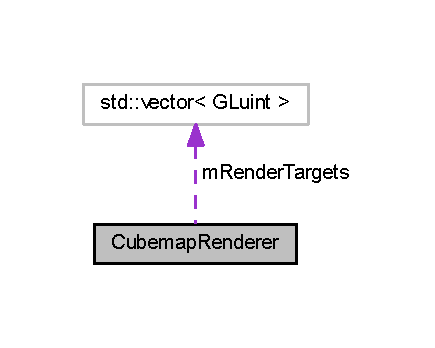
\includegraphics[width=209pt]{class_cubemap_renderer__coll__graph}
\end{center}
\end{figure}
\subsection*{Public Member Functions}
\begin{DoxyCompactItemize}
\item 
void \hyperlink{class_cubemap_renderer_aaaade77e14c75944a1dea1c809d777fb}{Begin} (int, G\+Luint, G\+Luint)
\item 
void {\bfseries End} (int)\hypertarget{class_cubemap_renderer_a9435e23f6aaab606ee0450d1909b560b}{}\label{class_cubemap_renderer_a9435e23f6aaab606ee0450d1909b560b}

\item 
std\+::vector$<$ G\+Luint $>$ {\bfseries get\+Render\+Targets} ()\hypertarget{class_cubemap_renderer_a0129da43b202da4263a6df388cf23355}{}\label{class_cubemap_renderer_a0129da43b202da4263a6df388cf23355}

\end{DoxyCompactItemize}
\subsection*{Data Fields}
\begin{DoxyCompactItemize}
\item 
std\+::shared\+\_\+ptr$<$ \hyperlink{class_shader}{Shader} $>$ {\bfseries m\+Main\+Shader}\hypertarget{class_cubemap_renderer_afdd2f628d718f612c16f2472221cc34d}{}\label{class_cubemap_renderer_afdd2f628d718f612c16f2472221cc34d}

\end{DoxyCompactItemize}
\subsection*{Private Member Functions}
\begin{DoxyCompactItemize}
\item 
void {\bfseries Copy\+Texture} (int)\hypertarget{class_cubemap_renderer_a7e8ccc9174fca56e9fe8ed7c92f912ff}{}\label{class_cubemap_renderer_a7e8ccc9174fca56e9fe8ed7c92f912ff}

\item 
void {\bfseries set\+Camera} ()\hypertarget{class_cubemap_renderer_a3c52ed27dbb4a9397be805b8add53c4b}{}\label{class_cubemap_renderer_a3c52ed27dbb4a9397be805b8add53c4b}

\end{DoxyCompactItemize}
\subsection*{Private Attributes}
\begin{DoxyCompactItemize}
\item 
float {\bfseries m\+N\+E\+AR}\hypertarget{class_cubemap_renderer_a86e41f5601710e0c8e50dcaa8bed103c}{}\label{class_cubemap_renderer_a86e41f5601710e0c8e50dcaa8bed103c}

\item 
float {\bfseries m\+F\+AR}\hypertarget{class_cubemap_renderer_a3cfe44c6e37d07f881ede9b53e5bc464}{}\label{class_cubemap_renderer_a3cfe44c6e37d07f881ede9b53e5bc464}

\item 
int {\bfseries m\+W\+I\+D\+TH}\hypertarget{class_cubemap_renderer_a3a51c98788a7b6c8a7d808ed7c0c6e49}{}\label{class_cubemap_renderer_a3a51c98788a7b6c8a7d808ed7c0c6e49}

\item 
int {\bfseries m\+H\+E\+I\+G\+HT}\hypertarget{class_cubemap_renderer_ab4b8f75ad23dcdd0e3c2c53e02a370d9}{}\label{class_cubemap_renderer_ab4b8f75ad23dcdd0e3c2c53e02a370d9}

\item 
glm\+::vec3 {\bfseries m\+Position}\hypertarget{class_cubemap_renderer_ab75b59ac05619624aee8a0211de352a5}{}\label{class_cubemap_renderer_ab75b59ac05619624aee8a0211de352a5}

\item 
std\+::shared\+\_\+ptr$<$ \hyperlink{class_frame_buffer}{Frame\+Buffer}$<$ int $>$ $>$ {\bfseries m\+Frame\+Buffer}\hypertarget{class_cubemap_renderer_ae19a90e9ca2c4006432761440039168f}{}\label{class_cubemap_renderer_ae19a90e9ca2c4006432761440039168f}

\item 
std\+::shared\+\_\+ptr$<$ \hyperlink{class_frame_buffer}{Frame\+Buffer}$<$ int $>$ $>$ {\bfseries m\+Copy\+Texture\+Frame\+Buffer}\hypertarget{class_cubemap_renderer_a555a5ed25b351bc4439bb8738c1a28fd}{}\label{class_cubemap_renderer_a555a5ed25b351bc4439bb8738c1a28fd}

\item 
std\+::shared\+\_\+ptr$<$ \hyperlink{class_open_g_l_helpers_1_1_full_screen_quad}{Open\+G\+L\+Helpers\+::\+Full\+Screen\+Quad} $>$ {\bfseries m\+Full\+Screen\+Quad}\hypertarget{class_cubemap_renderer_acf58d00882f70d5a6bac8466fbb93abb}{}\label{class_cubemap_renderer_acf58d00882f70d5a6bac8466fbb93abb}

\item 
std\+::shared\+\_\+ptr$<$ \hyperlink{class_shader}{Shader} $>$ {\bfseries m\+Pass\+Through\+Shader}\hypertarget{class_cubemap_renderer_aab76c4e9fe6d7cdcf4747a818b23af4e}{}\label{class_cubemap_renderer_aab76c4e9fe6d7cdcf4747a818b23af4e}

\item 
std\+::vector$<$ G\+Luint $>$ {\bfseries m\+Render\+Targets}\hypertarget{class_cubemap_renderer_a80c6716d65cd3d35eb13fa67966b08a8}{}\label{class_cubemap_renderer_a80c6716d65cd3d35eb13fa67966b08a8}

\item 
std\+::shared\+\_\+ptr$<$ \hyperlink{class_camera}{Camera} $>$ {\bfseries m\+Renderer\+Camera}\hypertarget{class_cubemap_renderer_a1410f13ffc4a96396a2984f89566e8ee}{}\label{class_cubemap_renderer_a1410f13ffc4a96396a2984f89566e8ee}

\end{DoxyCompactItemize}


\subsection{Detailed Description}


Definition at line 13 of file cubemap\+Renderer.\+h.



\subsection{Member Function Documentation}
\index{Cubemap\+Renderer@{Cubemap\+Renderer}!Begin@{Begin}}
\index{Begin@{Begin}!Cubemap\+Renderer@{Cubemap\+Renderer}}
\subsubsection[{\texorpdfstring{Begin(int, G\+Luint, G\+Luint)}{Begin(int, GLuint, GLuint)}}]{\setlength{\rightskip}{0pt plus 5cm}void Cubemap\+Renderer\+::\+Begin (
\begin{DoxyParamCaption}
\item[{int}]{index, }
\item[{G\+Luint}]{texture, }
\item[{G\+Luint}]{F\+BO}
\end{DoxyParamCaption}
)}\hypertarget{class_cubemap_renderer_aaaade77e14c75944a1dea1c809d777fb}{}\label{class_cubemap_renderer_aaaade77e14c75944a1dea1c809d777fb}
Function receives the current faces\textquotesingle{} index 

Definition at line 19 of file cubemap\+Renderer.\+cpp.


\hypertarget{class_physics_1_1_cube_physic_object}{}\section{Physics\+:\+:Cube\+Physic\+Object Class Reference}
\label{class_physics_1_1_cube_physic_object}\index{Physics\+::\+Cube\+Physic\+Object@{Physics\+::\+Cube\+Physic\+Object}}


Inheritance diagram for Physics\+:\+:Cube\+Physic\+Object\+:
\nopagebreak
\begin{figure}[H]
\begin{center}
\leavevmode
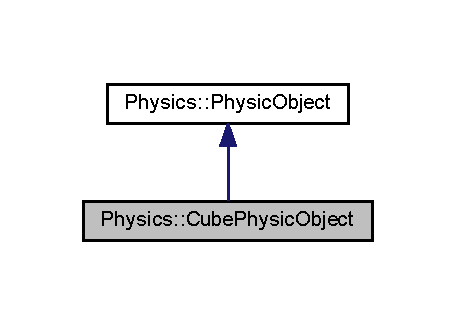
\includegraphics[width=219pt]{class_physics_1_1_cube_physic_object__inherit__graph}
\end{center}
\end{figure}


Collaboration diagram for Physics\+:\+:Cube\+Physic\+Object\+:
\nopagebreak
\begin{figure}[H]
\begin{center}
\leavevmode
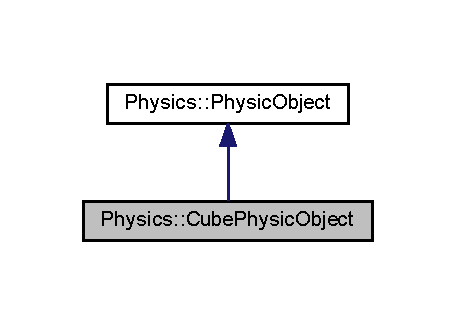
\includegraphics[width=219pt]{class_physics_1_1_cube_physic_object__coll__graph}
\end{center}
\end{figure}
\subsection*{Public Member Functions}
\begin{DoxyCompactItemize}
\item 
virtual std\+::shared\+\_\+ptr$<$ bt\+Rigid\+Body $>$ {\bfseries add\+Object} (float, float, float, float, float)\hypertarget{class_physics_1_1_cube_physic_object_a91256fe683984587eeaf484f95aece80}{}\label{class_physics_1_1_cube_physic_object_a91256fe683984587eeaf484f95aece80}

\item 
virtual std\+::shared\+\_\+ptr$<$ bt\+Rigid\+Body $>$ {\bfseries add\+Object} (glm\+::vec3, float, \hyperlink{struct_m_i_n___m_a_x___p_o_i_n_t_s}{M\+I\+N\+\_\+\+M\+A\+X\+\_\+\+P\+O\+I\+N\+TS}, float)\hypertarget{class_physics_1_1_cube_physic_object_a48ddcf7df0a08b934779509e39289942}{}\label{class_physics_1_1_cube_physic_object_a48ddcf7df0a08b934779509e39289942}

\end{DoxyCompactItemize}
\subsection*{Private Member Functions}
\begin{DoxyCompactItemize}
\item 
virtual std\+::shared\+\_\+ptr$<$ bt\+Rigid\+Body $>$ {\bfseries add\+Object} (float, float)\hypertarget{class_physics_1_1_cube_physic_object_a4f35f61329030f482bf6e2d2df850431}{}\label{class_physics_1_1_cube_physic_object_a4f35f61329030f482bf6e2d2df850431}

\item 
virtual std\+::shared\+\_\+ptr$<$ bt\+Rigid\+Body $>$ {\bfseries add\+Object} (std\+::vector$<$ glm\+::vec3 $>$, std\+::vector$<$ unsigned int $>$, float)\hypertarget{class_physics_1_1_cube_physic_object_a831e9b82a690bdb822b6ddd0ea81198a}{}\label{class_physics_1_1_cube_physic_object_a831e9b82a690bdb822b6ddd0ea81198a}

\item 
virtual std\+::shared\+\_\+ptr$<$ bt\+Rigid\+Body $>$ {\bfseries add\+Object} (glm\+::vec3, float, float)\hypertarget{class_physics_1_1_cube_physic_object_a35e7b5cfd0181501a5a831caa765112c}{}\label{class_physics_1_1_cube_physic_object_a35e7b5cfd0181501a5a831caa765112c}

\end{DoxyCompactItemize}
\subsection*{Private Attributes}
\begin{DoxyCompactItemize}
\item 
float {\bfseries m\+\_\+\+Size} = 1.\+0f\hypertarget{class_physics_1_1_cube_physic_object_a49edd861021c769d5d1d747043feb56a}{}\label{class_physics_1_1_cube_physic_object_a49edd861021c769d5d1d747043feb56a}

\item 
float {\bfseries m\+\_\+\+Mass} = 0.\+0f\hypertarget{class_physics_1_1_cube_physic_object_a6828f9bf568f840d07b853421c3876e1}{}\label{class_physics_1_1_cube_physic_object_a6828f9bf568f840d07b853421c3876e1}

\item 
glm\+::vec3 {\bfseries m\+\_\+\+Position} = glm\+::vec3(0.\+0f, 0.\+0f, 0.\+0f)\hypertarget{class_physics_1_1_cube_physic_object_a80de2908178c79d690b047676f96afe1}{}\label{class_physics_1_1_cube_physic_object_a80de2908178c79d690b047676f96afe1}

\item 
std\+::shared\+\_\+ptr$<$ bt\+Box\+Shape $>$ {\bfseries Cube\+Shape}\hypertarget{class_physics_1_1_cube_physic_object_ae0d63fbd5bc97dbd3c8c7e90be96e5e9}{}\label{class_physics_1_1_cube_physic_object_ae0d63fbd5bc97dbd3c8c7e90be96e5e9}

\item 
std\+::shared\+\_\+ptr$<$ bt\+Motion\+State $>$ {\bfseries motion\+State}\hypertarget{class_physics_1_1_cube_physic_object_a6441b26c2be6eff8cb5102e428ebf4ce}{}\label{class_physics_1_1_cube_physic_object_a6441b26c2be6eff8cb5102e428ebf4ce}

\item 
std\+::shared\+\_\+ptr$<$ bt\+Compound\+Shape $>$ {\bfseries m\+\_\+\+Col\+Shape}\hypertarget{class_physics_1_1_cube_physic_object_a3b70e8d67173fe57b2527ba6e22fc6e0}{}\label{class_physics_1_1_cube_physic_object_a3b70e8d67173fe57b2527ba6e22fc6e0}

\end{DoxyCompactItemize}
\subsection*{Additional Inherited Members}


\subsection{Detailed Description}


Definition at line 6 of file Cube\+Physic\+Object.\+h.


\hypertarget{struct_c_vector2}{}\section{C\+Vector2 Struct Reference}
\label{struct_c_vector2}\index{C\+Vector2@{C\+Vector2}}
\subsection*{Data Fields}
\begin{DoxyCompactItemize}
\item 
float {\bfseries x}\hypertarget{struct_c_vector2_a33cc20e661507c82c45d27e75563d672}{}\label{struct_c_vector2_a33cc20e661507c82c45d27e75563d672}

\item 
float {\bfseries y}\hypertarget{struct_c_vector2_a3856009668b0d289c514161ca5828e2a}{}\label{struct_c_vector2_a3856009668b0d289c514161ca5828e2a}

\end{DoxyCompactItemize}


\subsection{Detailed Description}


Definition at line 37 of file B\+S\+P.\+h.


\hypertarget{struct_c_vector3}{}\section{C\+Vector3 Struct Reference}
\label{struct_c_vector3}\index{C\+Vector3@{C\+Vector3}}
\subsection*{Data Fields}
\begin{DoxyCompactItemize}
\item 
float {\bfseries x}\hypertarget{struct_c_vector3_a06b092361b335f9971323be0ddf759b1}{}\label{struct_c_vector3_a06b092361b335f9971323be0ddf759b1}

\item 
float {\bfseries y}\hypertarget{struct_c_vector3_a20d0b1099477995b22a4f1407e41a7a1}{}\label{struct_c_vector3_a20d0b1099477995b22a4f1407e41a7a1}

\item 
float {\bfseries z}\hypertarget{struct_c_vector3_a9dd3ce85f6aaa17ccc67bfe50a089b3a}{}\label{struct_c_vector3_a9dd3ce85f6aaa17ccc67bfe50a089b3a}

\end{DoxyCompactItemize}


\subsection{Detailed Description}


Definition at line 32 of file B\+S\+P.\+h.


\hypertarget{class_d_d_s}{}\section{D\+DS Class Reference}
\label{class_d_d_s}\index{D\+DS@{D\+DS}}


Collaboration diagram for D\+DS\+:
\nopagebreak
\begin{figure}[H]
\begin{center}
\leavevmode
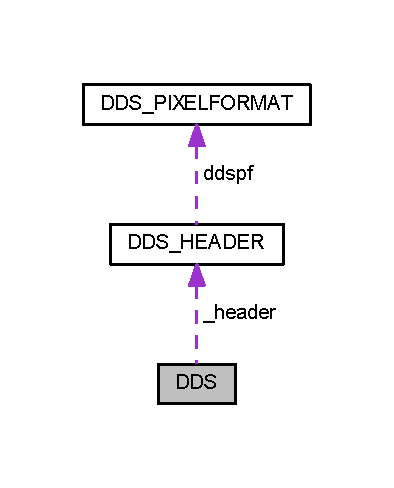
\includegraphics[width=189pt]{class_d_d_s__coll__graph}
\end{center}
\end{figure}
\subsection*{Public Member Functions}
\begin{DoxyCompactItemize}
\item 
{\bfseries D\+DS} (std\+::string)\hypertarget{class_d_d_s_ac5ac976521bebdef668de3e1cf77e279}{}\label{class_d_d_s_ac5ac976521bebdef668de3e1cf77e279}

\item 
const \hyperlink{struct_d_d_s___h_e_a_d_e_r}{D\+D\+S\+\_\+\+H\+E\+A\+D\+ER} $\ast$ {\bfseries header} () const \hypertarget{class_d_d_s_a7bac3c01274736d1a5fc85c807312f6b}{}\label{class_d_d_s_a7bac3c01274736d1a5fc85c807312f6b}

\item 
const std\+::shared\+\_\+ptr$<$ unsigned char $>$ {\bfseries Data} () const \hypertarget{class_d_d_s_a4cc8e7e708642b15b10ad5f9694a742c}{}\label{class_d_d_s_a4cc8e7e708642b15b10ad5f9694a742c}

\item 
const unsigned int {\bfseries Internal\+Format} () const \hypertarget{class_d_d_s_a958175f74602a608bc71e2928ec135fa}{}\label{class_d_d_s_a958175f74602a608bc71e2928ec135fa}

\end{DoxyCompactItemize}
\subsection*{Private Attributes}
\begin{DoxyCompactItemize}
\item 
\hyperlink{struct_d_d_s___h_e_a_d_e_r}{D\+D\+S\+\_\+\+H\+E\+A\+D\+ER} $\ast$ {\bfseries \+\_\+header}\hypertarget{class_d_d_s_a354ae60bdc35adf0b92e4d320e61fad6}{}\label{class_d_d_s_a354ae60bdc35adf0b92e4d320e61fad6}

\item 
std\+::shared\+\_\+ptr$<$ unsigned char $>$ {\bfseries data}\hypertarget{class_d_d_s_a4c9dc0548401f81bdfd8e799e1c15976}{}\label{class_d_d_s_a4c9dc0548401f81bdfd8e799e1c15976}

\item 
unsigned int {\bfseries m\+\_\+\+Internal\+Format}\hypertarget{class_d_d_s_a82a480e9bed9083c47312a60e7755248}{}\label{class_d_d_s_a82a480e9bed9083c47312a60e7755248}

\end{DoxyCompactItemize}


\subsection{Detailed Description}


Definition at line 4 of file D\+D\+S.\+h.


\hypertarget{class_i_o_1_1_image_1_1_d_d_s}{}\section{IO\+:\+:Image\+:\+:D\+DS Class Reference}
\label{class_i_o_1_1_image_1_1_d_d_s}\index{I\+O\+::\+Image\+::\+D\+DS@{I\+O\+::\+Image\+::\+D\+DS}}


Collaboration diagram for IO\+:\+:Image\+:\+:D\+DS\+:
\nopagebreak
\begin{figure}[H]
\begin{center}
\leavevmode
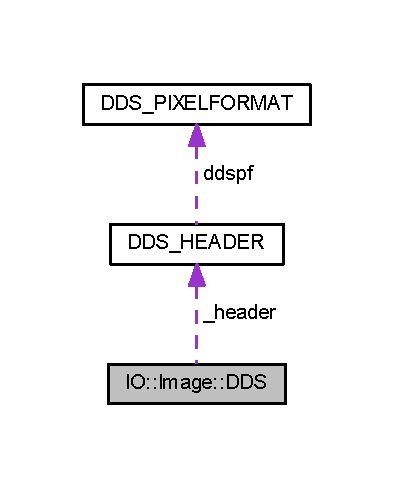
\includegraphics[width=189pt]{class_i_o_1_1_image_1_1_d_d_s__coll__graph}
\end{center}
\end{figure}
\subsection*{Public Member Functions}
\begin{DoxyCompactItemize}
\item 
{\bfseries D\+DS} (std\+::string)\hypertarget{class_i_o_1_1_image_1_1_d_d_s_ac5ac976521bebdef668de3e1cf77e279}{}\label{class_i_o_1_1_image_1_1_d_d_s_ac5ac976521bebdef668de3e1cf77e279}

\item 
const \hyperlink{struct_d_d_s___h_e_a_d_e_r}{D\+D\+S\+\_\+\+H\+E\+A\+D\+ER} $\ast$ {\bfseries header} () const \hypertarget{class_i_o_1_1_image_1_1_d_d_s_a6a15230421bf4b07a38029dae364808f}{}\label{class_i_o_1_1_image_1_1_d_d_s_a6a15230421bf4b07a38029dae364808f}

\item 
const std\+::shared\+\_\+ptr$<$ unsigned char $>$ {\bfseries Data} () const \hypertarget{class_i_o_1_1_image_1_1_d_d_s_ac4f120e5afbb940faffabbf7c705fdd7}{}\label{class_i_o_1_1_image_1_1_d_d_s_ac4f120e5afbb940faffabbf7c705fdd7}

\item 
const unsigned int {\bfseries Internal\+Format} () const \hypertarget{class_i_o_1_1_image_1_1_d_d_s_a32785a55a7a1267ff0c3bde1dfb8eb6f}{}\label{class_i_o_1_1_image_1_1_d_d_s_a32785a55a7a1267ff0c3bde1dfb8eb6f}

\end{DoxyCompactItemize}
\subsection*{Private Attributes}
\begin{DoxyCompactItemize}
\item 
\hyperlink{struct_d_d_s___h_e_a_d_e_r}{D\+D\+S\+\_\+\+H\+E\+A\+D\+ER} $\ast$ {\bfseries \+\_\+header}\hypertarget{class_i_o_1_1_image_1_1_d_d_s_a86d53fba767a3a2b7e6e8323ca642d6d}{}\label{class_i_o_1_1_image_1_1_d_d_s_a86d53fba767a3a2b7e6e8323ca642d6d}

\item 
std\+::shared\+\_\+ptr$<$ unsigned char $>$ {\bfseries data}\hypertarget{class_i_o_1_1_image_1_1_d_d_s_ad819b96494a8b89ae713a4b7434146ae}{}\label{class_i_o_1_1_image_1_1_d_d_s_ad819b96494a8b89ae713a4b7434146ae}

\item 
unsigned int {\bfseries m\+\_\+\+Internal\+Format}\hypertarget{class_i_o_1_1_image_1_1_d_d_s_abd54a124f39474a3ade09c62c66e338d}{}\label{class_i_o_1_1_image_1_1_d_d_s_abd54a124f39474a3ade09c62c66e338d}

\end{DoxyCompactItemize}


\subsection{Detailed Description}


Definition at line 6 of file D\+D\+S.\+h.


\hypertarget{struct_d_d_s___h_e_a_d_e_r}{}\section{D\+D\+S\+\_\+\+H\+E\+A\+D\+ER Struct Reference}
\label{struct_d_d_s___h_e_a_d_e_r}\index{D\+D\+S\+\_\+\+H\+E\+A\+D\+ER@{D\+D\+S\+\_\+\+H\+E\+A\+D\+ER}}


Collaboration diagram for D\+D\+S\+\_\+\+H\+E\+A\+D\+ER\+:
\nopagebreak
\begin{figure}[H]
\begin{center}
\leavevmode
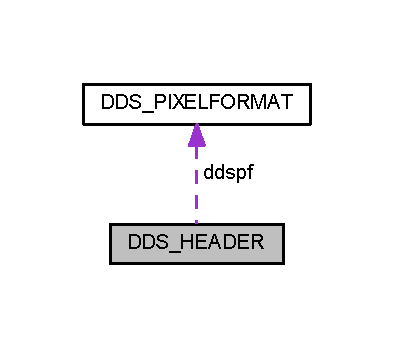
\includegraphics[width=189pt]{struct_d_d_s___h_e_a_d_e_r__coll__graph}
\end{center}
\end{figure}
\subsection*{Data Fields}
\begin{DoxyCompactItemize}
\item 
int {\bfseries dw\+Size}\hypertarget{struct_d_d_s___h_e_a_d_e_r_a383ba0dff0b7ecc076406e0032b5611f}{}\label{struct_d_d_s___h_e_a_d_e_r_a383ba0dff0b7ecc076406e0032b5611f}

\item 
int {\bfseries dw\+Flags}\hypertarget{struct_d_d_s___h_e_a_d_e_r_a9c8eaeba8d2c90b2378c5fc1c9e7956b}{}\label{struct_d_d_s___h_e_a_d_e_r_a9c8eaeba8d2c90b2378c5fc1c9e7956b}

\item 
int {\bfseries dw\+Height}\hypertarget{struct_d_d_s___h_e_a_d_e_r_a92c5c1384415aa817405fced60ff7b5a}{}\label{struct_d_d_s___h_e_a_d_e_r_a92c5c1384415aa817405fced60ff7b5a}

\item 
int {\bfseries dw\+Width}\hypertarget{struct_d_d_s___h_e_a_d_e_r_ac571f785c51a8c197b6fea3daf8360f0}{}\label{struct_d_d_s___h_e_a_d_e_r_ac571f785c51a8c197b6fea3daf8360f0}

\item 
int {\bfseries dw\+Pitch\+Or\+Linear\+Size}\hypertarget{struct_d_d_s___h_e_a_d_e_r_abd22b5a3079a03065bb3359104a87f2a}{}\label{struct_d_d_s___h_e_a_d_e_r_abd22b5a3079a03065bb3359104a87f2a}

\item 
int {\bfseries dw\+Depth}\hypertarget{struct_d_d_s___h_e_a_d_e_r_aff6df3f167394ea045d5fa511adfa53f}{}\label{struct_d_d_s___h_e_a_d_e_r_aff6df3f167394ea045d5fa511adfa53f}

\item 
int {\bfseries dw\+Mip\+Map\+Count}\hypertarget{struct_d_d_s___h_e_a_d_e_r_aa447e01b02f9ad7fb63499613f4e2e45}{}\label{struct_d_d_s___h_e_a_d_e_r_aa447e01b02f9ad7fb63499613f4e2e45}

\item 
int {\bfseries dw\+Reserved1} \mbox{[}11\mbox{]}\hypertarget{struct_d_d_s___h_e_a_d_e_r_a57f3120f4cbf14d9ae80ccd1fd95d88b}{}\label{struct_d_d_s___h_e_a_d_e_r_a57f3120f4cbf14d9ae80ccd1fd95d88b}

\item 
\hyperlink{struct_d_d_s___p_i_x_e_l_f_o_r_m_a_t}{D\+D\+S\+\_\+\+P\+I\+X\+E\+L\+F\+O\+R\+M\+AT} {\bfseries ddspf}\hypertarget{struct_d_d_s___h_e_a_d_e_r_a27445ea81444c05a620469f266bff154}{}\label{struct_d_d_s___h_e_a_d_e_r_a27445ea81444c05a620469f266bff154}

\item 
int {\bfseries dw\+Caps}\hypertarget{struct_d_d_s___h_e_a_d_e_r_a72545c3925fdab17734af8849e34006f}{}\label{struct_d_d_s___h_e_a_d_e_r_a72545c3925fdab17734af8849e34006f}

\item 
int {\bfseries dw\+Caps2}\hypertarget{struct_d_d_s___h_e_a_d_e_r_aaa67492946e0226c0d7a9856ff651f2e}{}\label{struct_d_d_s___h_e_a_d_e_r_aaa67492946e0226c0d7a9856ff651f2e}

\item 
int {\bfseries dw\+Caps3}\hypertarget{struct_d_d_s___h_e_a_d_e_r_a5e08cb4b384e154375c41c899b052c42}{}\label{struct_d_d_s___h_e_a_d_e_r_a5e08cb4b384e154375c41c899b052c42}

\item 
int {\bfseries dw\+Caps4}\hypertarget{struct_d_d_s___h_e_a_d_e_r_a8acdd296d7d53d39c989dcb56de783e2}{}\label{struct_d_d_s___h_e_a_d_e_r_a8acdd296d7d53d39c989dcb56de783e2}

\item 
int {\bfseries dw\+Reserved2}\hypertarget{struct_d_d_s___h_e_a_d_e_r_ac5b489890ce6f685967297b18f8c847c}{}\label{struct_d_d_s___h_e_a_d_e_r_ac5b489890ce6f685967297b18f8c847c}

\end{DoxyCompactItemize}


\subsection{Detailed Description}


Definition at line 22 of file D\+D\+S\+File.\+h.


\hypertarget{struct_d_d_s___p_i_x_e_l_f_o_r_m_a_t}{}\section{D\+D\+S\+\_\+\+P\+I\+X\+E\+L\+F\+O\+R\+M\+AT Struct Reference}
\label{struct_d_d_s___p_i_x_e_l_f_o_r_m_a_t}\index{D\+D\+S\+\_\+\+P\+I\+X\+E\+L\+F\+O\+R\+M\+AT@{D\+D\+S\+\_\+\+P\+I\+X\+E\+L\+F\+O\+R\+M\+AT}}
\subsection*{Data Fields}
\begin{DoxyCompactItemize}
\item 
int {\bfseries dw\+Size}\hypertarget{struct_d_d_s___p_i_x_e_l_f_o_r_m_a_t_a739655da318fe79bae54f19b04f3f8c5}{}\label{struct_d_d_s___p_i_x_e_l_f_o_r_m_a_t_a739655da318fe79bae54f19b04f3f8c5}

\item 
int {\bfseries dw\+Flags}\hypertarget{struct_d_d_s___p_i_x_e_l_f_o_r_m_a_t_ae92e157af09b1b4e635637ac33031ec8}{}\label{struct_d_d_s___p_i_x_e_l_f_o_r_m_a_t_ae92e157af09b1b4e635637ac33031ec8}

\item 
int {\bfseries dw\+Four\+CC}\hypertarget{struct_d_d_s___p_i_x_e_l_f_o_r_m_a_t_ab180a1787fcf6a6f6aec7179b9ac9b67}{}\label{struct_d_d_s___p_i_x_e_l_f_o_r_m_a_t_ab180a1787fcf6a6f6aec7179b9ac9b67}

\item 
int {\bfseries dw\+R\+G\+B\+Bit\+Count}\hypertarget{struct_d_d_s___p_i_x_e_l_f_o_r_m_a_t_ab419a113c34099904af5aaf09c243bcb}{}\label{struct_d_d_s___p_i_x_e_l_f_o_r_m_a_t_ab419a113c34099904af5aaf09c243bcb}

\item 
int {\bfseries dw\+R\+Bit\+Mask}\hypertarget{struct_d_d_s___p_i_x_e_l_f_o_r_m_a_t_a0badef2982a2b348111131b8a8464a3a}{}\label{struct_d_d_s___p_i_x_e_l_f_o_r_m_a_t_a0badef2982a2b348111131b8a8464a3a}

\item 
int {\bfseries dw\+G\+Bit\+Mask}\hypertarget{struct_d_d_s___p_i_x_e_l_f_o_r_m_a_t_aa63c6570e96e5e2bd01c661f0ee39030}{}\label{struct_d_d_s___p_i_x_e_l_f_o_r_m_a_t_aa63c6570e96e5e2bd01c661f0ee39030}

\item 
int {\bfseries dw\+B\+Bit\+Mask}\hypertarget{struct_d_d_s___p_i_x_e_l_f_o_r_m_a_t_a22cc6451146f3f6774654ee8c8fc72f5}{}\label{struct_d_d_s___p_i_x_e_l_f_o_r_m_a_t_a22cc6451146f3f6774654ee8c8fc72f5}

\item 
int {\bfseries dw\+A\+Bit\+Mask}\hypertarget{struct_d_d_s___p_i_x_e_l_f_o_r_m_a_t_ae08eb1a76181a3b3fabf65590c101b8c}{}\label{struct_d_d_s___p_i_x_e_l_f_o_r_m_a_t_ae08eb1a76181a3b3fabf65590c101b8c}

\end{DoxyCompactItemize}


\subsection{Detailed Description}


Definition at line 11 of file D\+D\+S\+File.\+h.


\hypertarget{class_deferred_renderer}{}\section{Deferred\+Renderer Class Reference}
\label{class_deferred_renderer}\index{Deferred\+Renderer@{Deferred\+Renderer}}


Inheritance diagram for Deferred\+Renderer\+:
\nopagebreak
\begin{figure}[H]
\begin{center}
\leavevmode
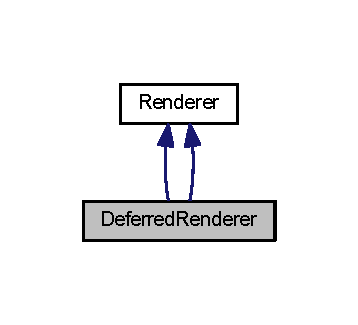
\includegraphics[width=172pt]{class_deferred_renderer__inherit__graph}
\end{center}
\end{figure}


Collaboration diagram for Deferred\+Renderer\+:
\nopagebreak
\begin{figure}[H]
\begin{center}
\leavevmode
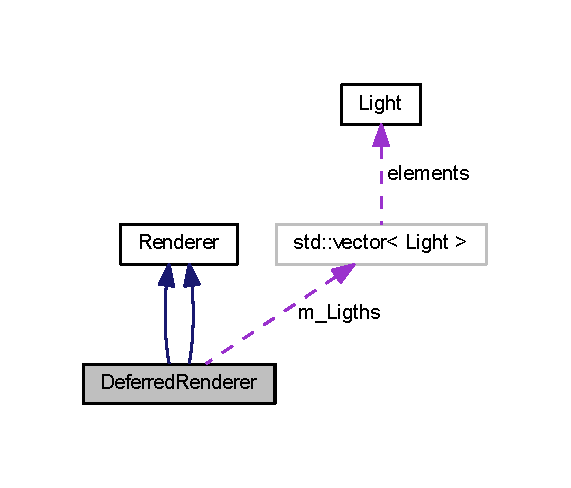
\includegraphics[width=274pt]{class_deferred_renderer__coll__graph}
\end{center}
\end{figure}
\subsection*{Public Member Functions}
\begin{DoxyCompactItemize}
\item 
virtual void {\bfseries Start} ()\hypertarget{class_deferred_renderer_a2c4c90972a828c3a360a56df41a277e6}{}\label{class_deferred_renderer_a2c4c90972a828c3a360a56df41a277e6}

\item 
virtual void {\bfseries End} ()\hypertarget{class_deferred_renderer_ac1cff7897713fc988112089ed6e7f514}{}\label{class_deferred_renderer_ac1cff7897713fc988112089ed6e7f514}

\item 
\hyperlink{class_deferred_renderer_a7ff36487b21145609eb8ba107d2e1db6}{Deferred\+Renderer} (int width, int height)
\item 
void {\bfseries begin\+Render} ()\hypertarget{class_deferred_renderer_a2f9c92eb5bc1a160805849b288ad98f0}{}\label{class_deferred_renderer_a2f9c92eb5bc1a160805849b288ad98f0}

\item 
void {\bfseries end\+Render} ()\hypertarget{class_deferred_renderer_a2c21b0833c7b57ce01dd3c5017875d78}{}\label{class_deferred_renderer_a2c21b0833c7b57ce01dd3c5017875d78}

\item 
void {\bfseries get\+Texture} ()\hypertarget{class_deferred_renderer_a49db94328fb391b443755af7b5e4342e}{}\label{class_deferred_renderer_a49db94328fb391b443755af7b5e4342e}

\end{DoxyCompactItemize}
\subsection*{Private Attributes}
\begin{DoxyCompactItemize}
\item 
std\+::vector$<$ \hyperlink{class_light}{Light} $>$ {\bfseries m\+\_\+\+Ligths}\hypertarget{class_deferred_renderer_a83ca815c8e8a8200bec7b36bb7236b72}{}\label{class_deferred_renderer_a83ca815c8e8a8200bec7b36bb7236b72}

\item 
std\+::shared\+\_\+ptr$<$ \hyperlink{class_frame_buffer}{Frame\+Buffer} $>$ {\bfseries m\+\_\+g\+Buffer}\hypertarget{class_deferred_renderer_a8c4cd8dfb136396766a5b84ddb182995}{}\label{class_deferred_renderer_a8c4cd8dfb136396766a5b84ddb182995}

\item 
std\+::shared\+\_\+ptr$<$ \hyperlink{class_frame_buffer}{Frame\+Buffer} $>$ {\bfseries m\+\_\+\+Composite\+Buffer}\hypertarget{class_deferred_renderer_a3045f0f36f06e7fd7915d4fc68907b5a}{}\label{class_deferred_renderer_a3045f0f36f06e7fd7915d4fc68907b5a}

\item 
std\+::shared\+\_\+ptr$<$ \hyperlink{class_shader}{Shader} $>$ {\bfseries m\+\_\+shader}\hypertarget{class_deferred_renderer_a867cac63d1b0a35b934f874442a0ec95}{}\label{class_deferred_renderer_a867cac63d1b0a35b934f874442a0ec95}

\item 
std\+::shared\+\_\+ptr$<$ e\+Camera $>$ {\bfseries m\+\_\+camera}\hypertarget{class_deferred_renderer_a6b87cec004bc40aebd34c4a25a036ea1}{}\label{class_deferred_renderer_a6b87cec004bc40aebd34c4a25a036ea1}

\end{DoxyCompactItemize}


\subsection{Detailed Description}


Definition at line 8 of file Deferred\+Renderer.\+h.



\subsection{Constructor \& Destructor Documentation}
\index{Deferred\+Renderer@{Deferred\+Renderer}!Deferred\+Renderer@{Deferred\+Renderer}}
\index{Deferred\+Renderer@{Deferred\+Renderer}!Deferred\+Renderer@{Deferred\+Renderer}}
\subsubsection[{\texorpdfstring{Deferred\+Renderer(int width, int height)}{DeferredRenderer(int width, int height)}}]{\setlength{\rightskip}{0pt plus 5cm}Deferred\+Renderer\+::\+Deferred\+Renderer (
\begin{DoxyParamCaption}
\item[{int}]{width, }
\item[{int}]{height}
\end{DoxyParamCaption}
)\hspace{0.3cm}{\ttfamily [inline]}}\hypertarget{class_deferred_renderer_a7ff36487b21145609eb8ba107d2e1db6}{}\label{class_deferred_renderer_a7ff36487b21145609eb8ba107d2e1db6}
Setting up the Geometry buffer

Setting up the composite buffer 

Definition at line 10 of file Deferred\+Renderer.\+h.


\hypertarget{class_post_process_1_1_effect}{}\section{Post\+Process\+:\+:Effect Class Reference}
\label{class_post_process_1_1_effect}\index{Post\+Process\+::\+Effect@{Post\+Process\+::\+Effect}}


Inheritance diagram for Post\+Process\+:\+:Effect\+:
\nopagebreak
\begin{figure}[H]
\begin{center}
\leavevmode
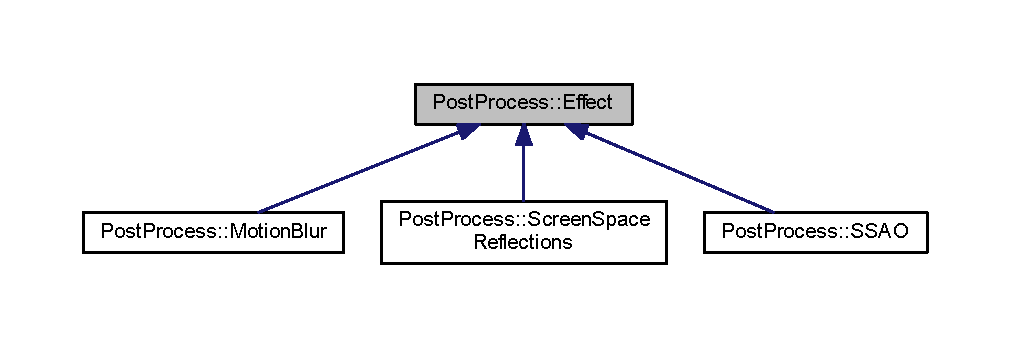
\includegraphics[width=350pt]{class_post_process_1_1_effect__inherit__graph}
\end{center}
\end{figure}
\subsection*{Public Member Functions}
\begin{DoxyCompactItemize}
\item 
{\bfseries Effect} (int, int)\hypertarget{class_post_process_1_1_effect_afbe32efd41c1801c3363e0e31afe57f5}{}\label{class_post_process_1_1_effect_afbe32efd41c1801c3363e0e31afe57f5}

\item 
virtual G\+Luint {\bfseries Apply} ()=0\hypertarget{class_post_process_1_1_effect_a1e09ae1bf1de1570aedbbf1a7fd4a7a5}{}\label{class_post_process_1_1_effect_a1e09ae1bf1de1570aedbbf1a7fd4a7a5}

\item 
virtual void {\bfseries Update} ()=0\hypertarget{class_post_process_1_1_effect_aec304379a238501f3d77530897e643b8}{}\label{class_post_process_1_1_effect_aec304379a238501f3d77530897e643b8}

\end{DoxyCompactItemize}
\subsection*{Protected Attributes}
\begin{DoxyCompactItemize}
\item 
std\+::shared\+\_\+ptr$<$ \hyperlink{class_frame_buffer}{Frame\+Buffer}$<$ std\+::string $>$ $>$ {\bfseries m\+\_\+p\+Frame\+Buffer}\hypertarget{class_post_process_1_1_effect_aa488936ef39986fab438ad778fdd1eb5}{}\label{class_post_process_1_1_effect_aa488936ef39986fab438ad778fdd1eb5}

\item 
std\+::shared\+\_\+ptr$<$ \hyperlink{class_open_g_l_helpers_1_1_full_screen_quad}{Open\+G\+L\+Helpers\+::\+Full\+Screen\+Quad} $>$ {\bfseries m\+\_\+p\+Full\+Screen\+Quad}\hypertarget{class_post_process_1_1_effect_ac048d2f0b7c2180359ea4416f6dc8b82}{}\label{class_post_process_1_1_effect_ac048d2f0b7c2180359ea4416f6dc8b82}

\item 
std\+::shared\+\_\+ptr$<$ \hyperlink{class_shader}{Shader} $>$ {\bfseries m\+\_\+p\+Shader}\hypertarget{class_post_process_1_1_effect_a2d04105296d1b8be2849e38be42f23f3}{}\label{class_post_process_1_1_effect_a2d04105296d1b8be2849e38be42f23f3}

\item 
int {\bfseries m\+\_\+\+Width}\hypertarget{class_post_process_1_1_effect_a0877d8b2d098049afacd836c4b5d4de7}{}\label{class_post_process_1_1_effect_a0877d8b2d098049afacd836c4b5d4de7}

\item 
int {\bfseries m\+\_\+\+Height}\hypertarget{class_post_process_1_1_effect_a43a25397d0d839d4d46e77df28a23aea}{}\label{class_post_process_1_1_effect_a43a25397d0d839d4d46e77df28a23aea}

\end{DoxyCompactItemize}


\subsection{Detailed Description}


Definition at line 10 of file Effect.\+h.


\hypertarget{class_helpers_1_1_elapsed_time}{}\section{Helpers\+:\+:Elapsed\+Time Class Reference}
\label{class_helpers_1_1_elapsed_time}\index{Helpers\+::\+Elapsed\+Time@{Helpers\+::\+Elapsed\+Time}}
\subsection*{Public Member Functions}
\begin{DoxyCompactItemize}
\item 
{\bfseries Elapsed\+Time} (float max\+Time\+Step=0.\+03333f)\hypertarget{class_helpers_1_1_elapsed_time_a6802c9506ea1d2984db2dfc853e69890}{}\label{class_helpers_1_1_elapsed_time_a6802c9506ea1d2984db2dfc853e69890}

\item 
float {\bfseries Get\+Elapsed\+Time} () const \hypertarget{class_helpers_1_1_elapsed_time_ab184519b80f819a5f18507b00194bdd6}{}\label{class_helpers_1_1_elapsed_time_ab184519b80f819a5f18507b00194bdd6}

\end{DoxyCompactItemize}
\subsection*{Private Attributes}
\begin{DoxyCompactItemize}
\item 
float {\bfseries m\+\_\+f\+Max\+Time\+Step}\hypertarget{class_helpers_1_1_elapsed_time_a2702d8a9f3bd81e3a4bf01e79150b636}{}\label{class_helpers_1_1_elapsed_time_a2702d8a9f3bd81e3a4bf01e79150b636}

\item 
float {\bfseries m\+\_\+f\+Previous}\hypertarget{class_helpers_1_1_elapsed_time_a8f97573e4c9f6e46ab25a2ab963f69ed}{}\label{class_helpers_1_1_elapsed_time_a8f97573e4c9f6e46ab25a2ab963f69ed}

\end{DoxyCompactItemize}


\subsection{Detailed Description}


Definition at line 205 of file Includes.\+h.


\hypertarget{class_entity_template}{}\section{Entity\+Template Class Reference}
\label{class_entity_template}\index{Entity\+Template@{Entity\+Template}}


Collaboration diagram for Entity\+Template\+:
\nopagebreak
\begin{figure}[H]
\begin{center}
\leavevmode
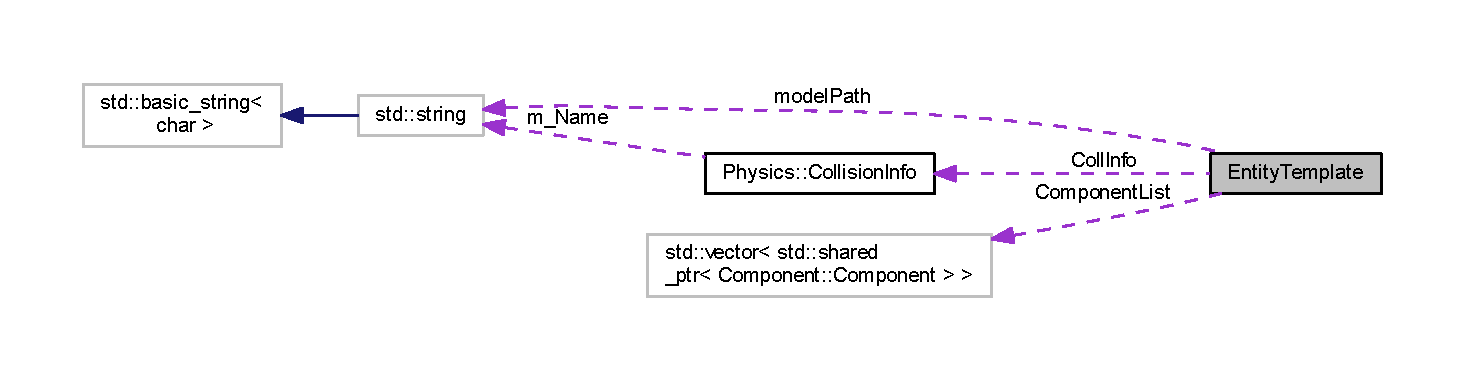
\includegraphics[width=350pt]{class_entity_template__coll__graph}
\end{center}
\end{figure}
\subsection*{Public Member Functions}
\begin{DoxyCompactItemize}
\item 
{\bfseries Entity\+Template} (std\+::shared\+\_\+ptr$<$ \hyperlink{class_resource_manager}{Resource\+Manager} $>$ rm, glm\+::vec3 pos, glm\+::vec3 sc, glm\+::quat rot)\hypertarget{class_entity_template_a835da6ccca2b8fbf53db7cb1ebffa85a}{}\label{class_entity_template_a835da6ccca2b8fbf53db7cb1ebffa85a}

\item 
void {\bfseries add\+Component} (std\+::shared\+\_\+ptr$<$ \hyperlink{class_component_1_1_component}{Component\+::\+Component} $>$ t)\hypertarget{class_entity_template_ac8321b22a8c2a781634850d9fab6df4e}{}\label{class_entity_template_ac8321b22a8c2a781634850d9fab6df4e}

\item 
void {\bfseries Update} ()\hypertarget{class_entity_template_a3d3a948716b31911b55f124f41994bb8}{}\label{class_entity_template_a3d3a948716b31911b55f124f41994bb8}

\item 
void {\bfseries Render} ()\hypertarget{class_entity_template_ac8ea339efcf5ccfdd4a9be8220830aef}{}\label{class_entity_template_ac8ea339efcf5ccfdd4a9be8220830aef}

\item 
void {\bfseries Render\+Shadows} ()\hypertarget{class_entity_template_aeff24e4911790a2c2f5a3f1044399a66}{}\label{class_entity_template_aeff24e4911790a2c2f5a3f1044399a66}

\item 
glm\+::vec3 {\bfseries get\+Position} ()\hypertarget{class_entity_template_a58b67e09dc139f0e6c524d13dffaa14d}{}\label{class_entity_template_a58b67e09dc139f0e6c524d13dffaa14d}

\item 
glm\+::vec3 {\bfseries get\+Prev\+Position} ()\hypertarget{class_entity_template_ab32c01732ae30bce09349205a5dcc15a}{}\label{class_entity_template_ab32c01732ae30bce09349205a5dcc15a}

\item 
glm\+::vec3 {\bfseries get\+Scale} ()\hypertarget{class_entity_template_a8d63187b137c8da1cc1b68a3b3a9b5d3}{}\label{class_entity_template_a8d63187b137c8da1cc1b68a3b3a9b5d3}

\item 
glm\+::vec3 {\bfseries get\+Prev\+Scale} ()\hypertarget{class_entity_template_ad2aa2fa03dbf878bfe81065564172b9c}{}\label{class_entity_template_ad2aa2fa03dbf878bfe81065564172b9c}

\item 
glm\+::quat {\bfseries get\+Rotation} ()\hypertarget{class_entity_template_af26ee422fd735162b8090d8942122cb7}{}\label{class_entity_template_af26ee422fd735162b8090d8942122cb7}

\item 
glm\+::quat {\bfseries get\+Prev\+Rotation} ()\hypertarget{class_entity_template_a27a0dd1dd7046c7c4aa7f1ff0cc06a50}{}\label{class_entity_template_a27a0dd1dd7046c7c4aa7f1ff0cc06a50}

\item 
\hyperlink{struct_m_i_n___m_a_x___p_o_i_n_t_s}{M\+I\+N\+\_\+\+M\+A\+X\+\_\+\+P\+O\+I\+N\+TS} {\bfseries get\+Bounding\+Box} ()\hypertarget{class_entity_template_ab78eb4367fea5a9df14386a9cbc0cdb6}{}\label{class_entity_template_ab78eb4367fea5a9df14386a9cbc0cdb6}

\item 
long {\bfseries to\+Hash} ()\hypertarget{class_entity_template_a172abb2b80217f33f5e0cf2ccd1bafeb}{}\label{class_entity_template_a172abb2b80217f33f5e0cf2ccd1bafeb}

\item 
void {\bfseries set\+Shader} (std\+::string sh)\hypertarget{class_entity_template_a2ccb14b558800599e0b7d5598afd4aca}{}\label{class_entity_template_a2ccb14b558800599e0b7d5598afd4aca}

\end{DoxyCompactItemize}
\subsection*{Data Fields}
\begin{DoxyCompactItemize}
\item 
bool {\bfseries has\+Player\+Component} = false\hypertarget{class_entity_template_a5fa22e1a9509c613f4e1346bf1748722}{}\label{class_entity_template_a5fa22e1a9509c613f4e1346bf1748722}

\item 
bool {\bfseries has\+Model} = false\hypertarget{class_entity_template_af2766cf841ba16dd64b7f2a1c1029a34}{}\label{class_entity_template_af2766cf841ba16dd64b7f2a1c1029a34}

\item 
bool {\bfseries has\+Physic\+Component} = false\hypertarget{class_entity_template_afd4bf4abe3b26adf9dbce131ead0593a}{}\label{class_entity_template_afd4bf4abe3b26adf9dbce131ead0593a}

\item 
bool {\bfseries has\+Cloth\+Component} = false\hypertarget{class_entity_template_a5c69077872edc24f0ef0847ee12fb6a7}{}\label{class_entity_template_a5c69077872edc24f0ef0847ee12fb6a7}

\item 
int {\bfseries ID}\hypertarget{class_entity_template_ad427cb58611f953613755f7771f2b608}{}\label{class_entity_template_ad427cb58611f953613755f7771f2b608}

\item 
std\+::string {\bfseries model\+Path}\hypertarget{class_entity_template_afdb73a0ce60c40aafa25a4b39f7c52db}{}\label{class_entity_template_afdb73a0ce60c40aafa25a4b39f7c52db}

\item 
std\+::vector$<$ std\+::shared\+\_\+ptr$<$ \hyperlink{class_component_1_1_component}{Component\+::\+Component} $>$ $>$ {\bfseries Component\+List}\hypertarget{class_entity_template_a43acb5764c2b2ade736859cd6174b367}{}\label{class_entity_template_a43acb5764c2b2ade736859cd6174b367}

\end{DoxyCompactItemize}
\subsection*{Private Attributes}
\begin{DoxyCompactItemize}
\item 
glm\+::vec3 {\bfseries m\+\_\+\+Position}\hypertarget{class_entity_template_a7d870912d0a3b6b12ea10f961a8dd6ff}{}\label{class_entity_template_a7d870912d0a3b6b12ea10f961a8dd6ff}

\item 
glm\+::vec3 {\bfseries m\+\_\+\+Scale}\hypertarget{class_entity_template_a74618b9555c8ba4026a822fa9ba907e6}{}\label{class_entity_template_a74618b9555c8ba4026a822fa9ba907e6}

\item 
glm\+::quat {\bfseries m\+\_\+\+Rotation}\hypertarget{class_entity_template_ad9095228ca57933e8e44fd09293ee553}{}\label{class_entity_template_ad9095228ca57933e8e44fd09293ee553}

\item 
glm\+::vec3 {\bfseries m\+\_\+\+Prev\+Position}\hypertarget{class_entity_template_a0e5349a4bc69b0b3a751ea0f5ee403fb}{}\label{class_entity_template_a0e5349a4bc69b0b3a751ea0f5ee403fb}

\item 
glm\+::vec3 {\bfseries m\+\_\+\+Prev\+Scale}\hypertarget{class_entity_template_a9900973652555a788884ae19a21f231b}{}\label{class_entity_template_a9900973652555a788884ae19a21f231b}

\item 
glm\+::quat {\bfseries m\+\_\+\+Prev\+Rotation}\hypertarget{class_entity_template_aa075496f781e0966ca16a0a12300bbf9}{}\label{class_entity_template_aa075496f781e0966ca16a0a12300bbf9}

\item 
\hyperlink{class_physics_1_1_collision_info}{Physics\+::\+Collision\+Info} {\bfseries Coll\+Info}\hypertarget{class_entity_template_a954a31be2af5f2c8ffee496443c50442}{}\label{class_entity_template_a954a31be2af5f2c8ffee496443c50442}

\item 
std\+::shared\+\_\+ptr$<$ \hyperlink{class_resource_manager}{Resource\+Manager} $>$ {\bfseries resource\+Manager}\hypertarget{class_entity_template_ab50f8e53879cb19aed028252cca762ac}{}\label{class_entity_template_ab50f8e53879cb19aed028252cca762ac}

\end{DoxyCompactItemize}


\subsection{Detailed Description}


Definition at line 11 of file Entity\+Template.\+h.


\hypertarget{class_epsilon}{}\section{Epsilon Class Reference}
\label{class_epsilon}\index{Epsilon@{Epsilon}}


Collaboration diagram for Epsilon\+:
\nopagebreak
\begin{figure}[H]
\begin{center}
\leavevmode
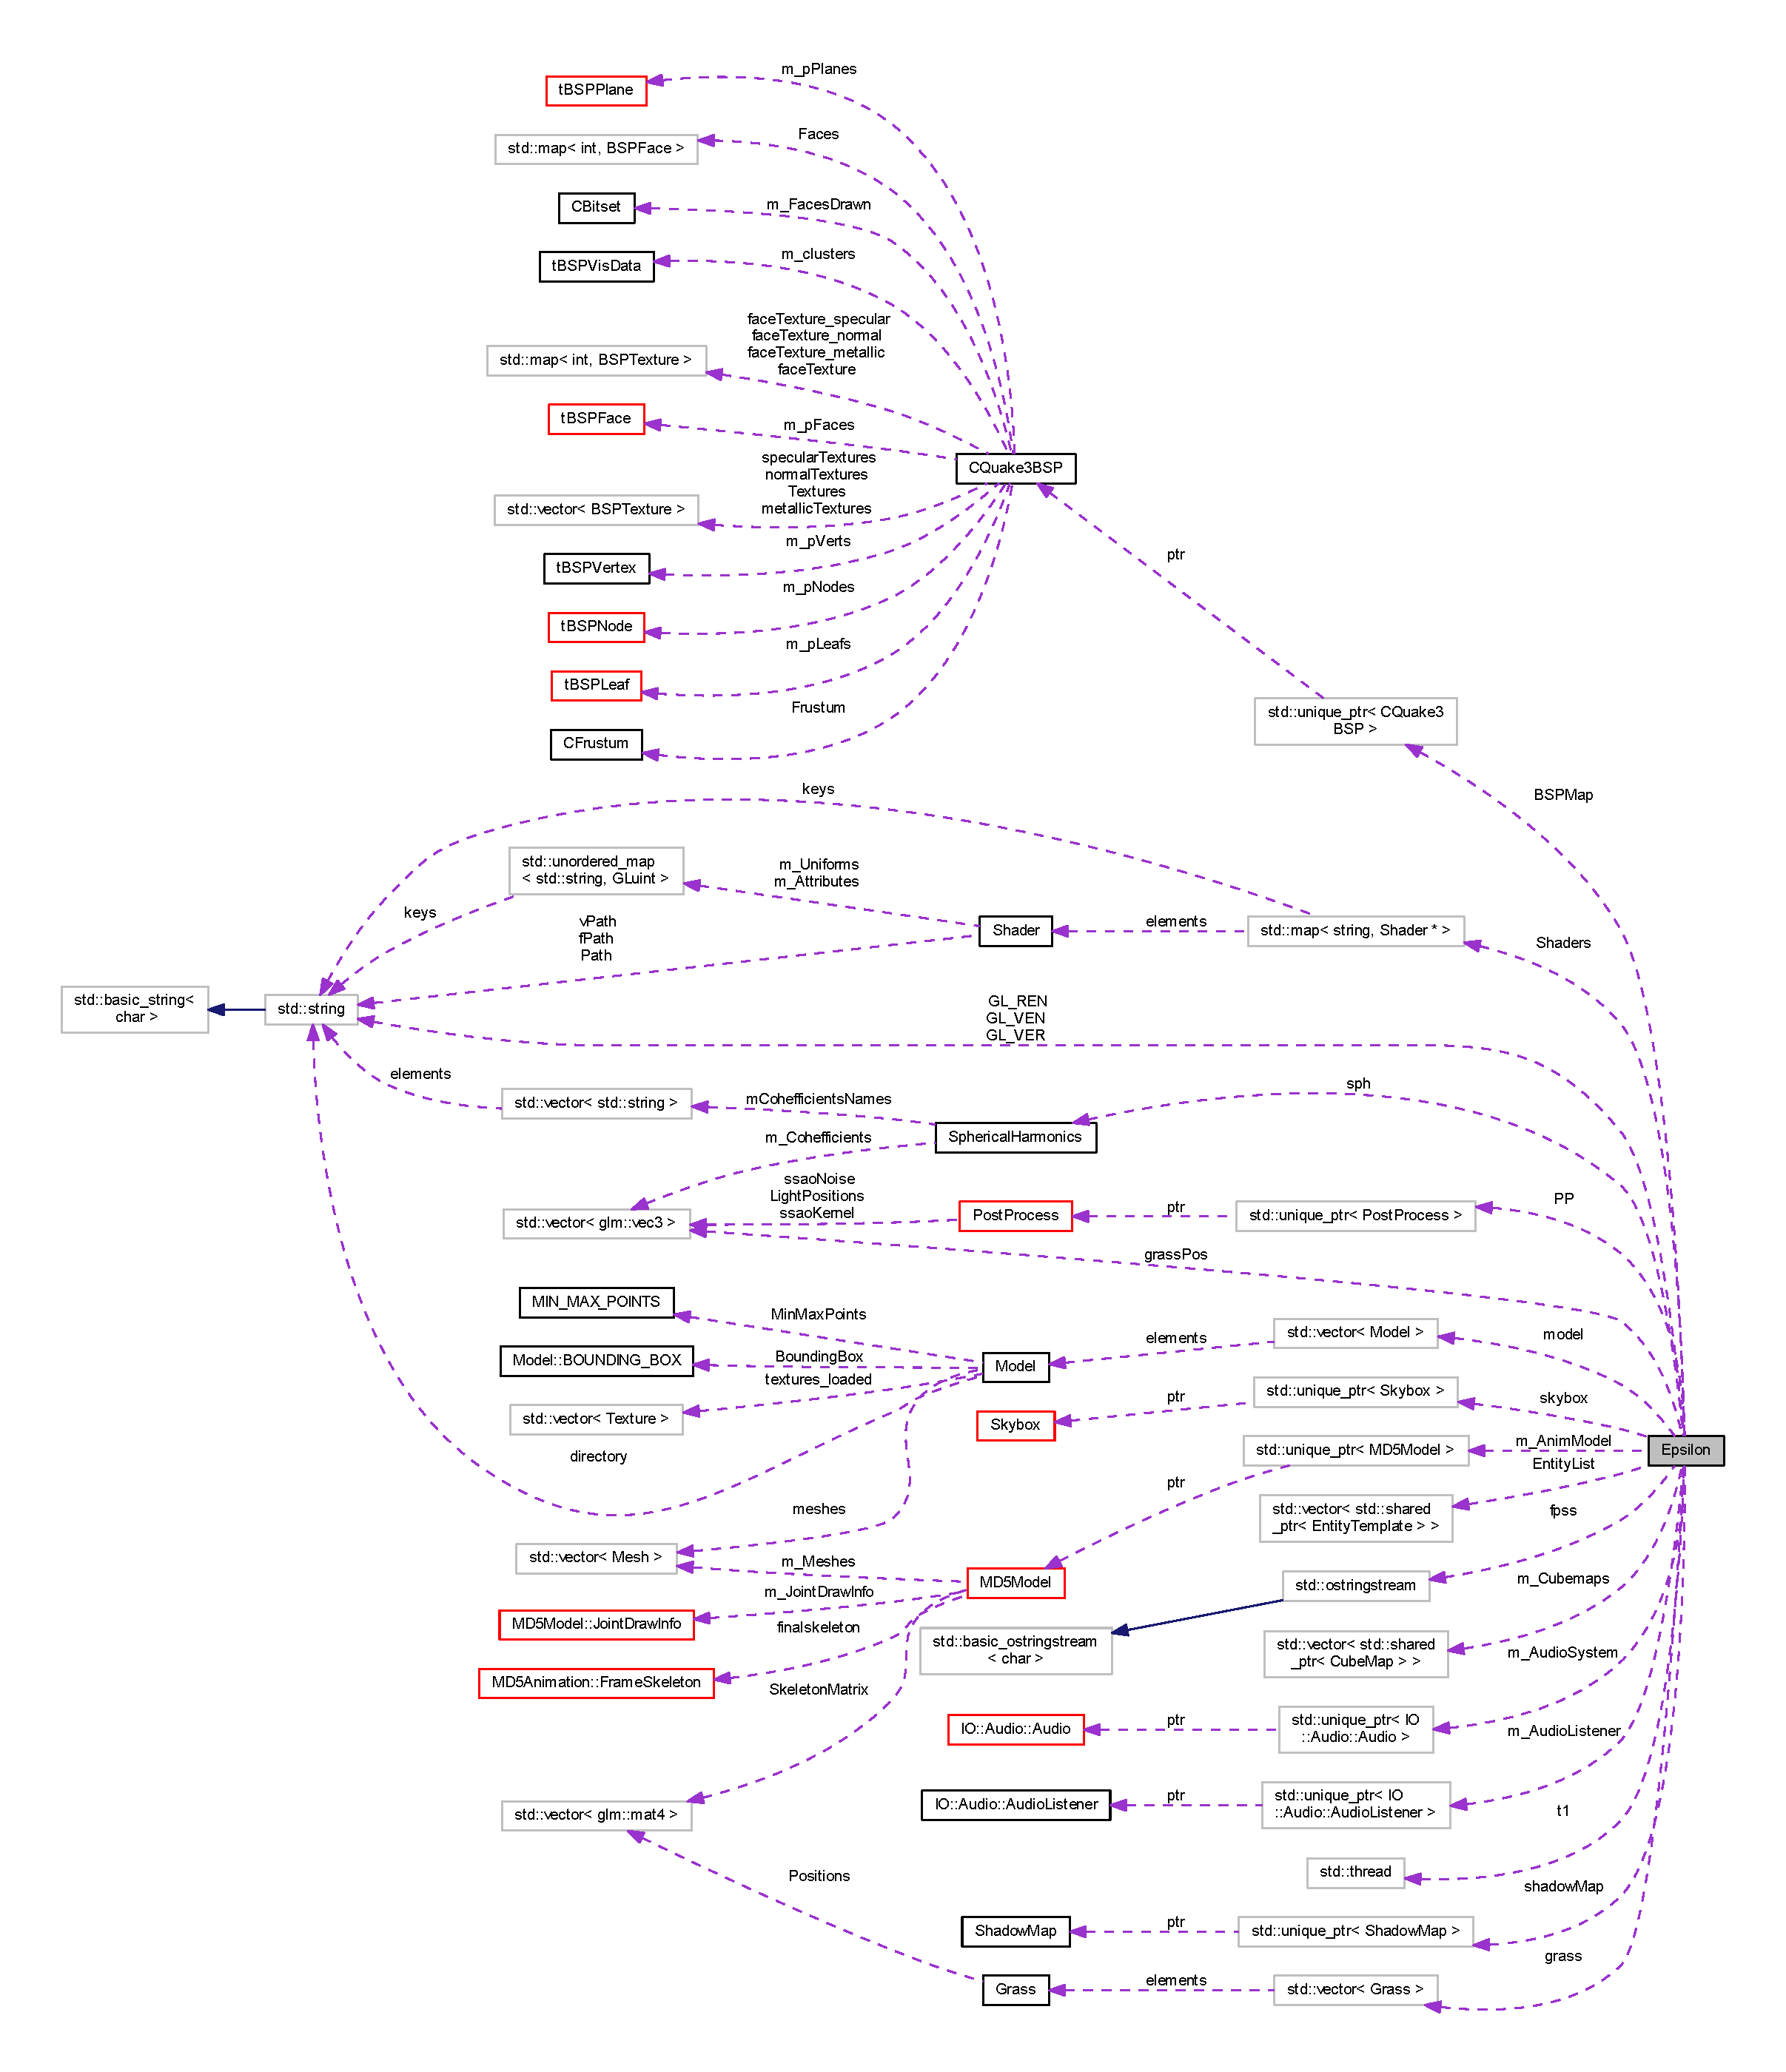
\includegraphics[width=350pt]{class_epsilon__coll__graph}
\end{center}
\end{figure}
\subsection*{Public Member Functions}
\begin{DoxyCompactItemize}
\item 
{\bfseries Epsilon} (G\+L\+F\+Wwindow $\ast$\&)\hypertarget{class_epsilon_a97302c6ca7b7d55d14f9ca742659ddca}{}\label{class_epsilon_a97302c6ca7b7d55d14f9ca742659ddca}

\item 
void {\bfseries Main\+Loop} (void)\hypertarget{class_epsilon_a2c59fe55bdbbfffbd7c3bca0532b4ec4}{}\label{class_epsilon_a2c59fe55bdbbfffbd7c3bca0532b4ec4}

\item 
void \hyperlink{class_epsilon_acdbbc212462949ba9bde213afc7b5a38}{Init\+Resources} (void)
\end{DoxyCompactItemize}
\subsection*{Data Fields}
\begin{DoxyCompactItemize}
\item 
std\+::shared\+\_\+ptr$<$ \hyperlink{class_camera}{Camera} $>$ {\bfseries e\+Camera}\hypertarget{class_epsilon_abfaacae6aa330a03d4c9ad5ea64e2a0c}{}\label{class_epsilon_abfaacae6aa330a03d4c9ad5ea64e2a0c}

\item 
std\+::shared\+\_\+ptr$<$ \hyperlink{class_physics_1_1_cloth_physic_object}{Physics\+::\+Cloth\+Physic\+Object} $>$ {\bfseries m\+Cloth}\hypertarget{class_epsilon_a201fc9489e5df35b08e7e88f26c05576}{}\label{class_epsilon_a201fc9489e5df35b08e7e88f26c05576}

\item 
std\+::shared\+\_\+ptr$<$ \hyperlink{class_patch}{Patch} $>$ {\bfseries m\+Patch}\hypertarget{class_epsilon_a42be8b163d188604f22956fec5228798}{}\label{class_epsilon_a42be8b163d188604f22956fec5228798}

\item 
G\+Luint \hyperlink{class_epsilon_a373ecfeb0f2da56ea44c70fd24a04a53}{cubemap\+Tex} = 0
\item 
G\+Luint {\bfseries cubemap\+Depth\+Tex} = 0\hypertarget{class_epsilon_a02bed2e9746800ffd4b355535b12abcc}{}\label{class_epsilon_a02bed2e9746800ffd4b355535b12abcc}

\item 
std\+::map$<$ string, \hyperlink{class_shader}{Shader} $\ast$ $>$ {\bfseries Shaders}\hypertarget{class_epsilon_a80c03a3455fad80a7e146ebb04a8a2fd}{}\label{class_epsilon_a80c03a3455fad80a7e146ebb04a8a2fd}

\item 
std\+::unique\+\_\+ptr$<$ \hyperlink{class_skybox}{Skybox} $>$ {\bfseries skybox}\hypertarget{class_epsilon_aa213c255e2fd3fde8d815106d193a031}{}\label{class_epsilon_aa213c255e2fd3fde8d815106d193a031}

\item 
std\+::shared\+\_\+ptr$<$ \hyperlink{class_water}{Water} $>$ {\bfseries water\+Plane}\hypertarget{class_epsilon_a6aa1464c9d08a34a80262f56f25efaff}{}\label{class_epsilon_a6aa1464c9d08a34a80262f56f25efaff}

\item 
std\+::vector$<$ \hyperlink{class_grass}{Grass} $>$ {\bfseries grass}\hypertarget{class_epsilon_ae0a6e3e7c24c4ea1ed750ffc039f5852}{}\label{class_epsilon_ae0a6e3e7c24c4ea1ed750ffc039f5852}

\item 
std\+::vector$<$ \hyperlink{class_model}{Model} $>$ {\bfseries model}\hypertarget{class_epsilon_a23cf64e07be032abc3ffe969f037c87b}{}\label{class_epsilon_a23cf64e07be032abc3ffe969f037c87b}

\item 
G\+Luint {\bfseries Vertex\+Array\+ID}\hypertarget{class_epsilon_acb637f14e1d02d3286d4021dd546fbef}{}\label{class_epsilon_acb637f14e1d02d3286d4021dd546fbef}

\item 
G\+L\+F\+Wwindow $\ast$ {\bfseries window} = nullptr\hypertarget{class_epsilon_a12aad9914ca9e20307ff65807b1db252}{}\label{class_epsilon_a12aad9914ca9e20307ff65807b1db252}

\item 
std\+::shared\+\_\+ptr$<$ \hyperlink{class_text}{Text} $>$ {\bfseries text}\hypertarget{class_epsilon_a43b14c92523a1fec14d475c2b50bc932}{}\label{class_epsilon_a43b14c92523a1fec14d475c2b50bc932}

\item 
std\+::shared\+\_\+ptr$<$ \hyperlink{class_terrain}{Terrain} $>$ {\bfseries terrain}\hypertarget{class_epsilon_a794ce0e478c5f087feb664bcb3abcb7c}{}\label{class_epsilon_a794ce0e478c5f087feb664bcb3abcb7c}

\item 
std\+::shared\+\_\+ptr$<$ \hyperlink{class_sun}{Sun} $>$ {\bfseries sun}\hypertarget{class_epsilon_a9123a170e3b6f0f345c7b76ccde79403}{}\label{class_epsilon_a9123a170e3b6f0f345c7b76ccde79403}

\item 
std\+::unique\+\_\+ptr$<$ \hyperlink{class_c_quake3_b_s_p}{C\+Quake3\+B\+SP} $>$ {\bfseries B\+S\+P\+Map}\hypertarget{class_epsilon_a4209ad5c3f4198bedc354a3f453b90f6}{}\label{class_epsilon_a4209ad5c3f4198bedc354a3f453b90f6}

\item 
std\+::unique\+\_\+ptr$<$ \hyperlink{class_m_d5_model}{M\+D5\+Model} $>$ {\bfseries m\+\_\+\+Anim\+Model}\hypertarget{class_epsilon_afb0e90e9c8c15c9091cbf6dea4500f53}{}\label{class_epsilon_afb0e90e9c8c15c9091cbf6dea4500f53}

\item 
std\+::unique\+\_\+ptr$<$ \hyperlink{class_shadow_map}{Shadow\+Map} $>$ {\bfseries shadow\+Map}\hypertarget{class_epsilon_a5cec8f0efb9c91fb2f61b20264e3ef8d}{}\label{class_epsilon_a5cec8f0efb9c91fb2f61b20264e3ef8d}

\item 
std\+::unique\+\_\+ptr$<$ \hyperlink{class_post_process}{Post\+Process} $>$ {\bfseries PP}\hypertarget{class_epsilon_a3522839e0199c6896e56e5ac9ee98550}{}\label{class_epsilon_a3522839e0199c6896e56e5ac9ee98550}

\item 
std\+::vector$<$ std\+::shared\+\_\+ptr$<$ \hyperlink{class_entity_template}{Entity\+Template} $>$ $>$ {\bfseries Entity\+List}\hypertarget{class_epsilon_a5bbbefe4de05db9e3a210447e7e341fa}{}\label{class_epsilon_a5bbbefe4de05db9e3a210447e7e341fa}

\item 
std\+::unique\+\_\+ptr$<$ \hyperlink{class_i_o_1_1_audio_1_1_audio}{I\+O\+::\+Audio\+::\+Audio} $>$ {\bfseries m\+\_\+\+Audio\+System}\hypertarget{class_epsilon_ad99e81e15f261af8afd61083dc314434}{}\label{class_epsilon_ad99e81e15f261af8afd61083dc314434}

\item 
std\+::unique\+\_\+ptr$<$ \hyperlink{class_i_o_1_1_audio_1_1_audio_listener}{I\+O\+::\+Audio\+::\+Audio\+Listener} $>$ {\bfseries m\+\_\+\+Audio\+Listener}\hypertarget{class_epsilon_a1023b5f96256fcdfe0efdd408dcf6ecd}{}\label{class_epsilon_a1023b5f96256fcdfe0efdd408dcf6ecd}

\item 
std\+::shared\+\_\+ptr$<$ \hyperlink{class_spherical_harmonics}{Spherical\+Harmonics} $>$ {\bfseries sphericalharmonics}\hypertarget{class_epsilon_a4a135163eeb3fb82c4fd3737a1060004}{}\label{class_epsilon_a4a135163eeb3fb82c4fd3737a1060004}

\item 
std\+::thread {\bfseries t1}\hypertarget{class_epsilon_a91b0fc4ff62151b96af0100e3afdb4b9}{}\label{class_epsilon_a91b0fc4ff62151b96af0100e3afdb4b9}

\item 
std\+::shared\+\_\+ptr$<$ \hyperlink{class_particle_system}{Particle\+System} $>$ {\bfseries m\+\_\+\+Particle\+System}\hypertarget{class_epsilon_abff74a16bcd1e516ee39a1aaa3d12d71}{}\label{class_epsilon_abff74a16bcd1e516ee39a1aaa3d12d71}

\item 
std\+::shared\+\_\+ptr$<$ \hyperlink{classe_texture}{e\+Texture} $>$ {\bfseries tex}\hypertarget{class_epsilon_a0bd1361123cdeceedcba1af257e5b66f}{}\label{class_epsilon_a0bd1361123cdeceedcba1af257e5b66f}

\item 
C\+A\+M\+E\+R\+A\+\_\+\+M\+O\+DE {\bfseries m\+\_\+\+Camera\+Mode}\hypertarget{class_epsilon_aeb2edd96204e1206a74faabdc22fba80}{}\label{class_epsilon_aeb2edd96204e1206a74faabdc22fba80}

\item 
std\+::vector$<$ std\+::shared\+\_\+ptr$<$ \hyperlink{class_cube_map}{Cube\+Map} $>$ $>$ {\bfseries m\+\_\+\+Cubemaps}\hypertarget{class_epsilon_ae69942651e2334e47772efd53b255615}{}\label{class_epsilon_ae69942651e2334e47772efd53b255615}

\item 
std\+::shared\+\_\+ptr$<$ \hyperlink{class_cube_map}{Cube\+Map} $>$ {\bfseries m\+Cubemap}\hypertarget{class_epsilon_ae29db1c10e659d5ebf99daf105e4809a}{}\label{class_epsilon_ae29db1c10e659d5ebf99daf105e4809a}

\item 
std\+::shared\+\_\+ptr$<$ \hyperlink{class_game_1_1_player}{Game\+::\+Player} $>$ {\bfseries m\+\_\+\+Player\+Capsule}\hypertarget{class_epsilon_a04665a1bb5a68ad3ce58da699e950eea}{}\label{class_epsilon_a04665a1bb5a68ad3ce58da699e950eea}

\item 
std\+::shared\+\_\+ptr$<$ \hyperlink{class_g_u_i}{G\+UI} $>$ {\bfseries m\+\_\+\+G\+UI}\hypertarget{class_epsilon_ac1ee53302ebb2b523ab9ce9d5b4085f8}{}\label{class_epsilon_ac1ee53302ebb2b523ab9ce9d5b4085f8}

\item 
std\+::shared\+\_\+ptr$<$ \hyperlink{class_panel}{Panel} $>$ {\bfseries m\+\_\+\+Panel}\hypertarget{class_epsilon_af9eeb9bfc7070eba5e0825bb0944d988}{}\label{class_epsilon_af9eeb9bfc7070eba5e0825bb0944d988}

\item 
std\+::shared\+\_\+ptr$<$ \hyperlink{class_button}{Button} $>$ {\bfseries t\+\_\+\+Button\+Settings}\hypertarget{class_epsilon_ab51b2a5e32060866cfa88636462ff60d}{}\label{class_epsilon_ab51b2a5e32060866cfa88636462ff60d}

\item 
std\+::shared\+\_\+ptr$<$ \hyperlink{class_panel}{Panel} $>$ {\bfseries t\+\_\+\+Panel\+Settings}\hypertarget{class_epsilon_aa2d01a0159b159ecf687c8a60d2e4e2a}{}\label{class_epsilon_aa2d01a0159b159ecf687c8a60d2e4e2a}

\item 
std\+::shared\+\_\+ptr$<$ \hyperlink{class_button}{Button} $>$ {\bfseries t\+\_\+\+Button\+Resume}\hypertarget{class_epsilon_aa6e4dbd8843cad591be006b21a0bfbf9}{}\label{class_epsilon_aa6e4dbd8843cad591be006b21a0bfbf9}

\item 
std\+::shared\+\_\+ptr$<$ \hyperlink{class_check_box}{Check\+Box} $>$ {\bfseries t\+\_\+\+Check\+Box}\hypertarget{class_epsilon_abb0ca9300f46b775efaa57383970c95e}{}\label{class_epsilon_abb0ca9300f46b775efaa57383970c95e}

\item 
bool {\bfseries Parallax\+On}\hypertarget{class_epsilon_aba41d13e40c2dc8796dc7da8b72274f0}{}\label{class_epsilon_aba41d13e40c2dc8796dc7da8b72274f0}

\item 
float \hyperlink{class_epsilon_aa59709ace8b71ed123e818708edc0543}{xz} \mbox{[}5\mbox{]}\mbox{[}5\mbox{]}
\item 
short {\bfseries W\+I\+D\+TH} = 16\hypertarget{class_epsilon_ad005199e74a13e0fc6dc1eb47416f073}{}\label{class_epsilon_ad005199e74a13e0fc6dc1eb47416f073}

\item 
short {\bfseries H\+E\+I\+G\+HT} = 16\hypertarget{class_epsilon_a7ad4ba1637a98f1def52a9488d3c69ac}{}\label{class_epsilon_a7ad4ba1637a98f1def52a9488d3c69ac}

\item 
bool {\bfseries S\+S\+AO} = false\hypertarget{class_epsilon_a40b12fc7256c567130cb22a4e3589436}{}\label{class_epsilon_a40b12fc7256c567130cb22a4e3589436}

\item 
double {\bfseries time\+Behind} = 0.\+0\hypertarget{class_epsilon_a7bf97215054ec71c0e8df83b53fede04}{}\label{class_epsilon_a7bf97215054ec71c0e8df83b53fede04}

\item 
float {\bfseries time\+G\+UI} = 0.\+0\hypertarget{class_epsilon_adc6c68c8ca9e97b9d90e6b965823367d}{}\label{class_epsilon_adc6c68c8ca9e97b9d90e6b965823367d}

\item 
\hyperlink{class_spherical_harmonics}{Spherical\+Harmonics} {\bfseries sph}\hypertarget{class_epsilon_ad818cadefca3345f9a1a1bdd82d3ae8e}{}\label{class_epsilon_ad818cadefca3345f9a1a1bdd82d3ae8e}

\item 
G\+Luint {\bfseries Ambient\+Light\+S\+S\+BO}\hypertarget{class_epsilon_a133e03db16b6866251a7c5e84df1cd55}{}\label{class_epsilon_a133e03db16b6866251a7c5e84df1cd55}

\end{DoxyCompactItemize}
\subsection*{Private Member Functions}
\begin{DoxyCompactItemize}
\item 
void \hyperlink{class_epsilon_a78c0240886a4a651bbd68f32a8a83bcb}{Load\+Geometry} (void)
\item 
void {\bfseries Load\+Sound} (void)\hypertarget{class_epsilon_af22c2e5923fcd5eef66d82b78ebaf45b}{}\label{class_epsilon_af22c2e5923fcd5eef66d82b78ebaf45b}

\item 
void {\bfseries Load\+Shaders} (void)\hypertarget{class_epsilon_a983a024c1507b66b8ac74319416dea46}{}\label{class_epsilon_a983a024c1507b66b8ac74319416dea46}

\item 
void {\bfseries Render\+Splash\+Screen} (std\+::string)\hypertarget{class_epsilon_aec29f963fbcfdb3aea13b88716160adb}{}\label{class_epsilon_aec29f963fbcfdb3aea13b88716160adb}

\item 
void {\bfseries Poll\+Events} (void)\hypertarget{class_epsilon_a755aeb43e7f4e87b93112ad0fa16b85f}{}\label{class_epsilon_a755aeb43e7f4e87b93112ad0fa16b85f}

\item 
void {\bfseries Render3D} (\hyperlink{class_shader}{Shader} $\ast$)\hypertarget{class_epsilon_ad7d2d1703bc1dd267a7ca64f15a34feb}{}\label{class_epsilon_ad7d2d1703bc1dd267a7ca64f15a34feb}

\item 
void {\bfseries Render3D} (void)\hypertarget{class_epsilon_a64c6ffc39309ac06ba984f676f34caa5}{}\label{class_epsilon_a64c6ffc39309ac06ba984f676f34caa5}

\item 
void {\bfseries Render2D} (void)\hypertarget{class_epsilon_affd17730239b1c11b926cee6f0e394a7}{}\label{class_epsilon_affd17730239b1c11b926cee6f0e394a7}

\item 
void {\bfseries Process\+Audio} (void)\hypertarget{class_epsilon_aa6a1cc4e2d5497023b197beaa621d79d}{}\label{class_epsilon_aa6a1cc4e2d5497023b197beaa621d79d}

\item 
void {\bfseries Render\+Legacy} (void)\hypertarget{class_epsilon_af2a8325d6788484ff3e6755504189253}{}\label{class_epsilon_af2a8325d6788484ff3e6755504189253}

\item 
void {\bfseries Render\+Skybox} (bool)\hypertarget{class_epsilon_aeb718827e14df8f618e362907c17f4be}{}\label{class_epsilon_aeb718827e14df8f618e362907c17f4be}

\item 
void {\bfseries Compute\+Water} (void)\hypertarget{class_epsilon_abbabb1ab313440119a0ff1741d52d4ca}{}\label{class_epsilon_abbabb1ab313440119a0ff1741d52d4ca}

\item 
void {\bfseries Swap\+Buffers} (void)\hypertarget{class_epsilon_a5e75d17eb31e4a826234b5611d2f710b}{}\label{class_epsilon_a5e75d17eb31e4a826234b5611d2f710b}

\item 
void {\bfseries Clear\+Buffers} (void)\hypertarget{class_epsilon_ac8ff48133df501675ef699c2e30d6c9c}{}\label{class_epsilon_ac8ff48133df501675ef699c2e30d6c9c}

\item 
void {\bfseries Compute\+Camera} (C\+A\+M\+E\+R\+A\+\_\+\+M\+O\+DE, glm\+::vec3 position=glm\+::vec3(0.\+0), glm\+::vec3 direction=glm\+::vec3(0.\+0), glm\+::mat4 proj=glm\+::mat4(0), glm\+::mat4 view=glm\+::mat4(0))\hypertarget{class_epsilon_a582383193c6b56f2ece5ba4e97bec2ca}{}\label{class_epsilon_a582383193c6b56f2ece5ba4e97bec2ca}

\item 
void {\bfseries Render\+Frame} (void)\hypertarget{class_epsilon_aec23d0bc6e70751880b20aa312e0e254}{}\label{class_epsilon_aec23d0bc6e70751880b20aa312e0e254}

\item 
void {\bfseries Process\+Frame} (void)\hypertarget{class_epsilon_a15d8da6ef70aabd9b8c13919bdf61bb2}{}\label{class_epsilon_a15d8da6ef70aabd9b8c13919bdf61bb2}

\item 
void {\bfseries Set\+Uniforms} (\hyperlink{class_shader}{Shader} $\ast$\&, glm\+::vec3 position, glm\+::vec3 scale, glm\+::quat rotation)\hypertarget{class_epsilon_ab7df71b81feb2a69c433d621c3b707c3}{}\label{class_epsilon_ab7df71b81feb2a69c433d621c3b707c3}

\item 
void {\bfseries Clock} (void)\hypertarget{class_epsilon_a485abd60922d9c5d1aabee3386b55266}{}\label{class_epsilon_a485abd60922d9c5d1aabee3386b55266}

\item 
void {\bfseries Compute\+Shadow} (void)\hypertarget{class_epsilon_a6b985dc929718148dc54490e34dbf21f}{}\label{class_epsilon_a6b985dc929718148dc54490e34dbf21f}

\item 
void {\bfseries Render\+To\+Cubemaps} ()\hypertarget{class_epsilon_ac696918509d18b87f1610cc5b4765418}{}\label{class_epsilon_ac696918509d18b87f1610cc5b4765418}

\item 
void {\bfseries Render\+Particles} ()\hypertarget{class_epsilon_acfb308b991cd8ffa1767b8244ecf88a1}{}\label{class_epsilon_acfb308b991cd8ffa1767b8244ecf88a1}

\end{DoxyCompactItemize}
\subsection*{Private Attributes}
\begin{DoxyCompactItemize}
\item 
bool {\bfseries normal} = 0\hypertarget{class_epsilon_a13ee7dfbabe704b302a60dad62f54615}{}\label{class_epsilon_a13ee7dfbabe704b302a60dad62f54615}

\item 
bool {\bfseries flash\+Light} = 0\hypertarget{class_epsilon_aa9924c414ff6240268212fa2b7aa3f2d}{}\label{class_epsilon_aa9924c414ff6240268212fa2b7aa3f2d}

\item 
bool {\bfseries hdr} = true\hypertarget{class_epsilon_a5501cf7542b772a09cf4d4d90a9bb998}{}\label{class_epsilon_a5501cf7542b772a09cf4d4d90a9bb998}

\item 
double {\bfseries last\+Time} = 0\hypertarget{class_epsilon_a01da56903e0602a9b075f35e1c54daca}{}\label{class_epsilon_a01da56903e0602a9b075f35e1c54daca}

\item 
double {\bfseries frametime} = 0\hypertarget{class_epsilon_a02eeaebcbdc08c1fba79f2da3f131b89}{}\label{class_epsilon_a02eeaebcbdc08c1fba79f2da3f131b89}

\item 
double {\bfseries etime} = 0\hypertarget{class_epsilon_a490cfdcf7c8055841a2c84c9351f8cd7}{}\label{class_epsilon_a490cfdcf7c8055841a2c84c9351f8cd7}

\item 
float {\bfseries wind\+Speed} = 0.\+0\hypertarget{class_epsilon_a8528e4671facd79090b4fa15374919ed}{}\label{class_epsilon_a8528e4671facd79090b4fa15374919ed}

\item 
float {\bfseries exposure} = 0\hypertarget{class_epsilon_a536df7a1ddb765cb5e66134b800e3b77}{}\label{class_epsilon_a536df7a1ddb765cb5e66134b800e3b77}

\item 
bool {\bfseries parallax} = false\hypertarget{class_epsilon_a337e26c855ae67cb3d45af0f2566001c}{}\label{class_epsilon_a337e26c855ae67cb3d45af0f2566001c}

\item 
float {\bfseries eventtime} = 0\hypertarget{class_epsilon_a4c11e8a8f223c276ee6777d8d8a9d133}{}\label{class_epsilon_a4c11e8a8f223c276ee6777d8d8a9d133}

\item 
short {\bfseries fps} = 0\hypertarget{class_epsilon_a6eda8c6f3d7757e0ff3f03bc83ae48cc}{}\label{class_epsilon_a6eda8c6f3d7757e0ff3f03bc83ae48cc}

\item 
int {\bfseries Frame\+Count} = 0\hypertarget{class_epsilon_a48b91fd667f11574b7a822dd018251f6}{}\label{class_epsilon_a48b91fd667f11574b7a822dd018251f6}

\item 
int {\bfseries Frames\+Since\+Last\+U\+I\+Update} = 0\hypertarget{class_epsilon_a5fccca83cb7117596c6871424049e3fe}{}\label{class_epsilon_a5fccca83cb7117596c6871424049e3fe}

\item 
bool {\bfseries showtext} = false\hypertarget{class_epsilon_a5c56615886879536842f8511c9c1cd94}{}\label{class_epsilon_a5c56615886879536842f8511c9c1cd94}

\item 
bool {\bfseries on\+Menu} = false\hypertarget{class_epsilon_add6a62776d73af7786cc116b07dc2b22}{}\label{class_epsilon_add6a62776d73af7786cc116b07dc2b22}

\item 
float {\bfseries menu\+Time} = 0.\+0\hypertarget{class_epsilon_a2bc93af33dc0013fa82dfe19d62effff}{}\label{class_epsilon_a2bc93af33dc0013fa82dfe19d62effff}

\item 
std\+::vector$<$ glm\+::vec3 $>$ {\bfseries grass\+Pos}\hypertarget{class_epsilon_ac96f8c02f0e5a73154e7036c7fb79450}{}\label{class_epsilon_ac96f8c02f0e5a73154e7036c7fb79450}

\item 
std\+::ostringstream {\bfseries fpss}\hypertarget{class_epsilon_a8f6ec2cc773f0a8a20b9293a1d59d8d9}{}\label{class_epsilon_a8f6ec2cc773f0a8a20b9293a1d59d8d9}

\item 
std\+::shared\+\_\+ptr$<$ \hyperlink{class_resource_manager}{Resource\+Manager} $>$ {\bfseries rM}\hypertarget{class_epsilon_aed713f9eef6e236d05ed4b2a36aab155}{}\label{class_epsilon_aed713f9eef6e236d05ed4b2a36aab155}

\item 
std\+::shared\+\_\+ptr$<$ \hyperlink{class_physics_1_1_sphere_physic_object}{Physics\+::\+Sphere\+Physic\+Object} $>$ {\bfseries ph3}\hypertarget{class_epsilon_a923fb68faf4526bf2bfdb7762ab2d566}{}\label{class_epsilon_a923fb68faf4526bf2bfdb7762ab2d566}

\item 
std\+::string {\bfseries G\+L\+\_\+\+V\+ER}\hypertarget{class_epsilon_a63563c9cfb97f4db51652ed1f44fb285}{}\label{class_epsilon_a63563c9cfb97f4db51652ed1f44fb285}

\item 
std\+::string {\bfseries G\+L\+\_\+\+R\+EN}\hypertarget{class_epsilon_a89e2eabfed6ef8a789cd289fc3e863a3}{}\label{class_epsilon_a89e2eabfed6ef8a789cd289fc3e863a3}

\item 
std\+::string {\bfseries G\+L\+\_\+\+V\+EN}\hypertarget{class_epsilon_a875c9b74238e12cdc5757b8c30e92982}{}\label{class_epsilon_a875c9b74238e12cdc5757b8c30e92982}

\item 
double {\bfseries m\+\_\+\+Text\+Acum} = 0.\+0\hypertarget{class_epsilon_a268f6d00f1aefae8a22cd94e9082ed18}{}\label{class_epsilon_a268f6d00f1aefae8a22cd94e9082ed18}

\end{DoxyCompactItemize}


\subsection{Detailed Description}


Definition at line 57 of file Epsilon.\+h.



\subsection{Member Function Documentation}
\index{Epsilon@{Epsilon}!Init\+Resources@{Init\+Resources}}
\index{Init\+Resources@{Init\+Resources}!Epsilon@{Epsilon}}
\subsubsection[{\texorpdfstring{Init\+Resources(void)}{InitResources(void)}}]{\setlength{\rightskip}{0pt plus 5cm}void Epsilon\+::\+Init\+Resources (
\begin{DoxyParamCaption}
\item[{void}]{}
\end{DoxyParamCaption}
)}\hypertarget{class_epsilon_acdbbc212462949ba9bde213afc7b5a38}{}\label{class_epsilon_acdbbc212462949ba9bde213afc7b5a38}
godrays tutorial begin

godrays tutorial end 

Definition at line 139 of file Epsilon.\+cpp.

\index{Epsilon@{Epsilon}!Load\+Geometry@{Load\+Geometry}}
\index{Load\+Geometry@{Load\+Geometry}!Epsilon@{Epsilon}}
\subsubsection[{\texorpdfstring{Load\+Geometry(void)}{LoadGeometry(void)}}]{\setlength{\rightskip}{0pt plus 5cm}void Epsilon\+::\+Load\+Geometry (
\begin{DoxyParamCaption}
\item[{void}]{}
\end{DoxyParamCaption}
)\hspace{0.3cm}{\ttfamily [private]}}\hypertarget{class_epsilon_a78c0240886a4a651bbd68f32a8a83bcb}{}\label{class_epsilon_a78c0240886a4a651bbd68f32a8a83bcb}
-\/11.\+8 

Definition at line 674 of file Epsilon.\+cpp.



\subsection{Field Documentation}
\index{Epsilon@{Epsilon}!cubemap\+Tex@{cubemap\+Tex}}
\index{cubemap\+Tex@{cubemap\+Tex}!Epsilon@{Epsilon}}
\subsubsection[{\texorpdfstring{cubemap\+Tex}{cubemapTex}}]{\setlength{\rightskip}{0pt plus 5cm}G\+Luint Epsilon\+::cubemap\+Tex = 0}\hypertarget{class_epsilon_a373ecfeb0f2da56ea44c70fd24a04a53}{}\label{class_epsilon_a373ecfeb0f2da56ea44c70fd24a04a53}
Shaders 

Definition at line 143 of file Epsilon.\+h.

\index{Epsilon@{Epsilon}!xz@{xz}}
\index{xz@{xz}!Epsilon@{Epsilon}}
\subsubsection[{\texorpdfstring{xz}{xz}}]{\setlength{\rightskip}{0pt plus 5cm}float Epsilon\+::xz\mbox{[}5\mbox{]}\mbox{[}5\mbox{]}}\hypertarget{class_epsilon_aa59709ace8b71ed123e818708edc0543}{}\label{class_epsilon_aa59709ace8b71ed123e818708edc0543}
Window Properties 

Definition at line 181 of file Epsilon.\+h.


\hypertarget{classe_texture}{}\section{e\+Texture Class Reference}
\label{classe_texture}\index{e\+Texture@{e\+Texture}}


Collaboration diagram for e\+Texture\+:
\nopagebreak
\begin{figure}[H]
\begin{center}
\leavevmode
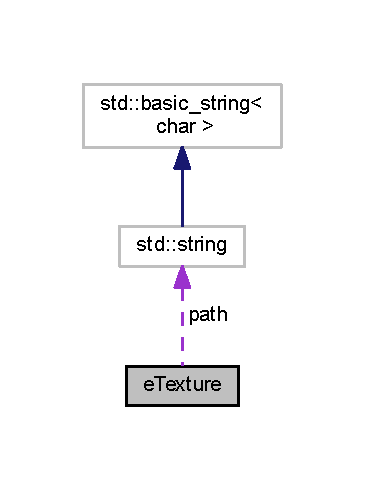
\includegraphics[width=175pt]{classe_texture__coll__graph}
\end{center}
\end{figure}
\subsection*{Public Member Functions}
\begin{DoxyCompactItemize}
\item 
{\bfseries e\+Texture} (const char $\ast$Tex\+Name, G\+Lenum wrap=G\+L\+\_\+\+R\+E\+P\+E\+AT, G\+Lenum type=G\+L\+\_\+\+T\+E\+X\+T\+U\+R\+E\+\_\+2D, G\+Luint filtering=-\/1)\hypertarget{classe_texture_a9ec24a2a3a66ef1a3b01f3a771678cd0}{}\label{classe_texture_a9ec24a2a3a66ef1a3b01f3a771678cd0}

\item 
{\bfseries e\+Texture} (std\+::vector$<$ std\+::string $>$ Cube\+Map\+Path)\hypertarget{classe_texture_aeafb4e7b82a31dc25568b682afbbdbfd}{}\label{classe_texture_aeafb4e7b82a31dc25568b682afbbdbfd}

\item 
void {\bfseries create\+Null\+Texture} (const char $\ast$Tex\+Name, G\+Lenum wrap=G\+L\+\_\+\+R\+E\+P\+E\+AT, G\+Lenum type=G\+L\+\_\+\+T\+E\+X\+T\+U\+R\+E\+\_\+2D, G\+Luint filtering=-\/1)\hypertarget{classe_texture_a83ddd5b62c54b797fc280525df59cd3b}{}\label{classe_texture_a83ddd5b62c54b797fc280525df59cd3b}

\item 
void {\bfseries create\+G\+L\+Texture} (unsigned char $\ast$image, const char $\ast$Tex\+Name, G\+Lenum wrap=G\+L\+\_\+\+R\+E\+P\+E\+AT, G\+Lenum type=G\+L\+\_\+\+T\+E\+X\+T\+U\+R\+E\+\_\+2D, G\+Luint filtering=-\/1)\hypertarget{classe_texture_a7b3ac2468c3742bcaf750321b7d3da08}{}\label{classe_texture_a7b3ac2468c3742bcaf750321b7d3da08}

\item 
void {\bfseries load\+File} (const char $\ast$path, unsigned char $\ast$\&data, int $\ast$outwidth, int $\ast$outheight, int $\ast$outchannels)\hypertarget{classe_texture_a58994ab16a3e5a5a799347b452639cfe}{}\label{classe_texture_a58994ab16a3e5a5a799347b452639cfe}

\item 
bool {\bfseries is\+Normal} (const char $\ast$Tex\+Name)\hypertarget{classe_texture_afeb634ec4c3c0b50f47419586c9865d3}{}\label{classe_texture_afeb634ec4c3c0b50f47419586c9865d3}

\item 
void {\bfseries Destroy} ()\hypertarget{classe_texture_a6e35d16487176c7374bcb4278e63d49d}{}\label{classe_texture_a6e35d16487176c7374bcb4278e63d49d}

\item 
G\+Luint {\bfseries get\+Texture\+ID} (void)\hypertarget{classe_texture_a533898fcfffcc4bc44900a5332d0263b}{}\label{classe_texture_a533898fcfffcc4bc44900a5332d0263b}

\item 
int {\bfseries get\+Width} ()\hypertarget{classe_texture_aee25d33f8fdd1169dd38a7205be9a199}{}\label{classe_texture_aee25d33f8fdd1169dd38a7205be9a199}

\item 
int {\bfseries get\+Height} ()\hypertarget{classe_texture_abb1dbcb9479bdd601b7fda6f19eafc9a}{}\label{classe_texture_abb1dbcb9479bdd601b7fda6f19eafc9a}

\item 
const char $\ast$ {\bfseries get\+Path} ()\hypertarget{classe_texture_a07f3dc41b4314f889e099f84c51372fe}{}\label{classe_texture_a07f3dc41b4314f889e099f84c51372fe}

\item 
void {\bfseries set\+Request\+Count} ()\hypertarget{classe_texture_a7c7632c6985463d2612888b14b604764}{}\label{classe_texture_a7c7632c6985463d2612888b14b604764}

\item 
void {\bfseries reset\+Request\+Count} ()\hypertarget{classe_texture_a8cebd725a5fd104e55e2c0d0113a8fa3}{}\label{classe_texture_a8cebd725a5fd104e55e2c0d0113a8fa3}

\item 
int {\bfseries get\+Times\+Used} ()\hypertarget{classe_texture_aefc9b33a8052f58bc7ffc9dfdc0b7947}{}\label{classe_texture_aefc9b33a8052f58bc7ffc9dfdc0b7947}

\item 
long {\bfseries to\+Hash} ()\hypertarget{classe_texture_a1994858c4811cb5308dfdfa248601199}{}\label{classe_texture_a1994858c4811cb5308dfdfa248601199}

\item 
void {\bfseries check\+Loading} ()\hypertarget{classe_texture_af4afd9082c1cf2b77da2cf8d07a20f93}{}\label{classe_texture_af4afd9082c1cf2b77da2cf8d07a20f93}

\end{DoxyCompactItemize}
\subsection*{Private Attributes}
\begin{DoxyCompactItemize}
\item 
G\+Luint {\bfseries texture} = 0\hypertarget{classe_texture_ad971f45612dacb43ca0d7c15ae756f1d}{}\label{classe_texture_ad971f45612dacb43ca0d7c15ae756f1d}

\item 
bool {\bfseries ispng} = false\hypertarget{classe_texture_ab3cb12de02f93a233af596ade029a198}{}\label{classe_texture_ab3cb12de02f93a233af596ade029a198}

\item 
bool {\bfseries m\+Loaded} = false\hypertarget{classe_texture_afd1aa1585fb7feddc59d36b51844f2aa}{}\label{classe_texture_afd1aa1585fb7feddc59d36b51844f2aa}

\item 
std\+::shared\+\_\+ptr$<$ \hyperlink{class_i_o_1_1_image_1_1_image}{I\+O\+::\+Image\+::\+Image} $>$ {\bfseries m\+Image} = nullptr\hypertarget{classe_texture_a558fbc7ce2ab879f6c76bd87130c5487}{}\label{classe_texture_a558fbc7ce2ab879f6c76bd87130c5487}

\item 
unsigned char $\ast$ {\bfseries image}\hypertarget{classe_texture_a30335ac7950cd767cf4aa2b8013cc1c0}{}\label{classe_texture_a30335ac7950cd767cf4aa2b8013cc1c0}

\item 
std\+::string {\bfseries path}\hypertarget{classe_texture_aa6eaae046d23ecfa2d957ec1255b9c86}{}\label{classe_texture_aa6eaae046d23ecfa2d957ec1255b9c86}

\item 
int {\bfseries m\+\_\+\+Times\+Used} = 0\hypertarget{classe_texture_afb728f12c3c2ab27fbb59c8bcb652eb3}{}\label{classe_texture_afb728f12c3c2ab27fbb59c8bcb652eb3}

\item 
double {\bfseries m\+\_\+\+Time\+Since\+Last\+Use} = 0.\+0\hypertarget{classe_texture_a6b9bbf09f6b63a36afc6ee0e18aced0e}{}\label{classe_texture_a6b9bbf09f6b63a36afc6ee0e18aced0e}

\item 
int {\bfseries width} = 0\hypertarget{classe_texture_ac01c2228b2de88acd9441de9d094f8af}{}\label{classe_texture_ac01c2228b2de88acd9441de9d094f8af}

\item 
int {\bfseries height} = 0\hypertarget{classe_texture_a607169804cdbbc9e4adb3211efd91cd0}{}\label{classe_texture_a607169804cdbbc9e4adb3211efd91cd0}

\end{DoxyCompactItemize}


\subsection{Detailed Description}


Definition at line 25 of file Texture.\+h.


\hypertarget{struct_face}{}\section{Face Struct Reference}
\label{struct_face}\index{Face@{Face}}
\subsection*{Data Fields}
\begin{DoxyCompactItemize}
\item 
glm\+::vec3 {\bfseries vertex0}\hypertarget{struct_face_a8803c329f74eb6b2f3839114c2946bc3}{}\label{struct_face_a8803c329f74eb6b2f3839114c2946bc3}

\item 
glm\+::vec3 {\bfseries vertex1}\hypertarget{struct_face_a587a818a98e51b0f48aba21dfca29bda}{}\label{struct_face_a587a818a98e51b0f48aba21dfca29bda}

\item 
glm\+::vec3 {\bfseries vertex2}\hypertarget{struct_face_a1e98ca0f2f18fd0e50e99844b92459e6}{}\label{struct_face_a1e98ca0f2f18fd0e50e99844b92459e6}

\end{DoxyCompactItemize}


\subsection{Detailed Description}


Definition at line 35 of file Terrain.\+h.


\hypertarget{class_i_o_1_1_filesystem_1_1_file}{}\section{IO\+:\+:Filesystem\+:\+:File Class Reference}
\label{class_i_o_1_1_filesystem_1_1_file}\index{I\+O\+::\+Filesystem\+::\+File@{I\+O\+::\+Filesystem\+::\+File}}


Collaboration diagram for IO\+:\+:Filesystem\+:\+:File\+:
\nopagebreak
\begin{figure}[H]
\begin{center}
\leavevmode
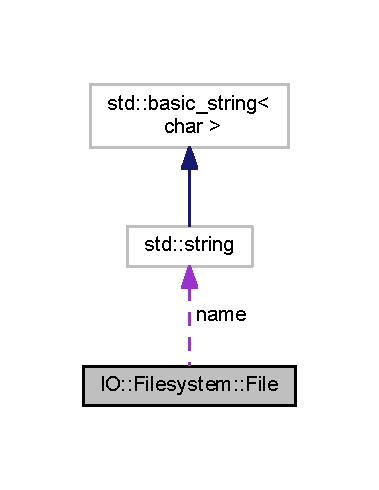
\includegraphics[width=182pt]{class_i_o_1_1_filesystem_1_1_file__coll__graph}
\end{center}
\end{figure}
\subsection*{Public Member Functions}
\begin{DoxyCompactItemize}
\item 
uint32\+\_\+t \hyperlink{class_i_o_1_1_filesystem_1_1_file_a162b7a834aa2880ffb57e64b61dafa62}{generate\+Hash} (std\+::string filename)
\end{DoxyCompactItemize}
\subsection*{Data Fields}
\begin{DoxyCompactItemize}
\item 
std\+::string {\bfseries name}\hypertarget{class_i_o_1_1_filesystem_1_1_file_a86d7c0717bd76958de8d105512c0920c}{}\label{class_i_o_1_1_filesystem_1_1_file_a86d7c0717bd76958de8d105512c0920c}

\item 
uint32\+\_\+t {\bfseries hash}\hypertarget{class_i_o_1_1_filesystem_1_1_file_aad4382da3abd369b7bf95ec45df02bf1}{}\label{class_i_o_1_1_filesystem_1_1_file_aad4382da3abd369b7bf95ec45df02bf1}

\item 
uint32\+\_\+t {\bfseries type}\hypertarget{class_i_o_1_1_filesystem_1_1_file_aa65b54894d2b1626619c0921bb8c957a}{}\label{class_i_o_1_1_filesystem_1_1_file_aa65b54894d2b1626619c0921bb8c957a}

\end{DoxyCompactItemize}


\subsection{Detailed Description}


Definition at line 22 of file filesystem.\+h.



\subsection{Member Function Documentation}
\index{I\+O\+::\+Filesystem\+::\+File@{I\+O\+::\+Filesystem\+::\+File}!generate\+Hash@{generate\+Hash}}
\index{generate\+Hash@{generate\+Hash}!I\+O\+::\+Filesystem\+::\+File@{I\+O\+::\+Filesystem\+::\+File}}
\subsubsection[{\texorpdfstring{generate\+Hash(std\+::string filename)}{generateHash(std::string filename)}}]{\setlength{\rightskip}{0pt plus 5cm}uint32\+\_\+t I\+O\+::\+Filesystem\+::\+File\+::generate\+Hash (
\begin{DoxyParamCaption}
\item[{std\+::string}]{filename}
\end{DoxyParamCaption}
)}\hypertarget{class_i_o_1_1_filesystem_1_1_file_a162b7a834aa2880ffb57e64b61dafa62}{}\label{class_i_o_1_1_filesystem_1_1_file_a162b7a834aa2880ffb57e64b61dafa62}
Theorical definition of a file including a hash in case it is inside a zip file and the name of the file itself 

Definition at line 13 of file filesystem.\+cpp.


\hypertarget{class_i_o_1_1_filesystem_1_1_filesystem}{}\section{IO\+:\+:Filesystem\+:\+:Filesystem Class Reference}
\label{class_i_o_1_1_filesystem_1_1_filesystem}\index{I\+O\+::\+Filesystem\+::\+Filesystem@{I\+O\+::\+Filesystem\+::\+Filesystem}}


Collaboration diagram for IO\+:\+:Filesystem\+:\+:Filesystem\+:
\nopagebreak
\begin{figure}[H]
\begin{center}
\leavevmode
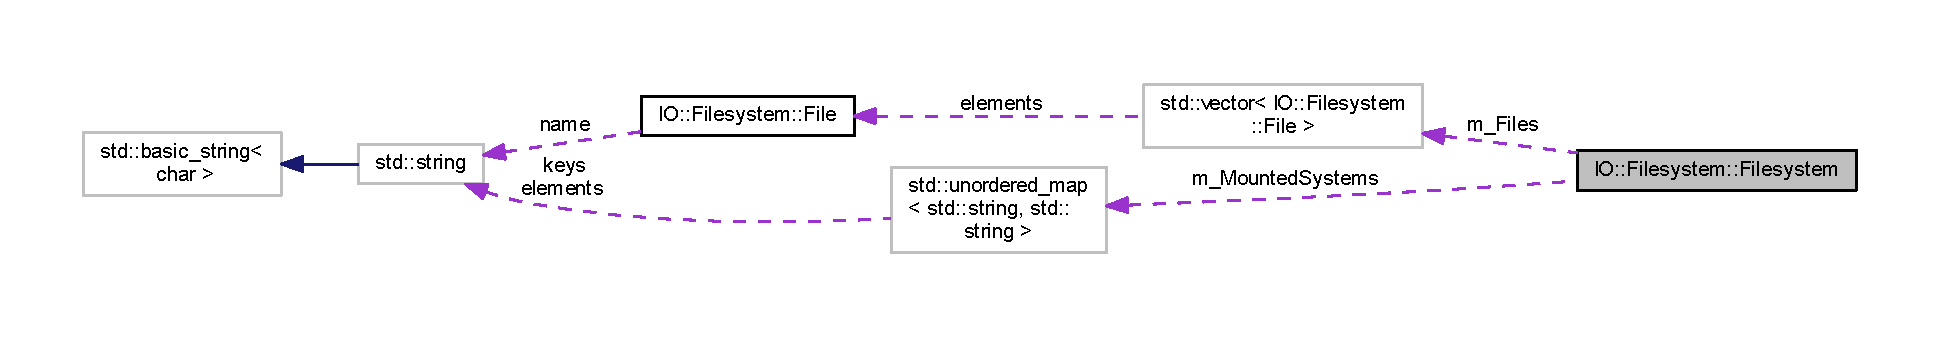
\includegraphics[width=350pt]{class_i_o_1_1_filesystem_1_1_filesystem__coll__graph}
\end{center}
\end{figure}
\subsection*{Public Member Functions}
\begin{DoxyCompactItemize}
\item 
const std\+::vector$<$ std\+::string $>$ \hyperlink{class_i_o_1_1_filesystem_1_1_filesystem_a08a55eab2acbf4868339d2dee3e861e6}{get\+File\+Names\+In\+Directory} (std\+::string, std\+::string)
\item 
bool {\bfseries File\+Exists} (std\+::string)\hypertarget{class_i_o_1_1_filesystem_1_1_filesystem_a8652e75765bc28f5d5f8da64ae8770f9}{}\label{class_i_o_1_1_filesystem_1_1_filesystem_a8652e75765bc28f5d5f8da64ae8770f9}

\item 
bool {\bfseries Mount} (std\+::string, std\+::string)\hypertarget{class_i_o_1_1_filesystem_1_1_filesystem_a82571e9965f36d7593a383fef2489e64}{}\label{class_i_o_1_1_filesystem_1_1_filesystem_a82571e9965f36d7593a383fef2489e64}

\item 
bool {\bfseries File\+System\+Is\+Zip} (\hyperlink{class_i_o_1_1_filesystem_1_1_file}{File} file)\hypertarget{class_i_o_1_1_filesystem_1_1_filesystem_afe8e55d51bd27cefd17c52ae62be79e6}{}\label{class_i_o_1_1_filesystem_1_1_filesystem_afe8e55d51bd27cefd17c52ae62be79e6}

\end{DoxyCompactItemize}
\subsection*{Private Attributes}
\begin{DoxyCompactItemize}
\item 
std\+::unordered\+\_\+map$<$ std\+::string, std\+::string $>$ {\bfseries m\+\_\+\+Mounted\+Systems}\hypertarget{class_i_o_1_1_filesystem_1_1_filesystem_ac71a116e35d3243ea9b8747b32439e01}{}\label{class_i_o_1_1_filesystem_1_1_filesystem_ac71a116e35d3243ea9b8747b32439e01}

\item 
std\+::vector$<$ \hyperlink{class_i_o_1_1_filesystem_1_1_file}{File} $>$ {\bfseries m\+\_\+\+Files}\hypertarget{class_i_o_1_1_filesystem_1_1_filesystem_adf20c9d57de39dcea58bcace45cbb5a9}{}\label{class_i_o_1_1_filesystem_1_1_filesystem_adf20c9d57de39dcea58bcace45cbb5a9}

\end{DoxyCompactItemize}


\subsection{Detailed Description}


Definition at line 63 of file filesystem.\+h.



\subsection{Member Function Documentation}
\index{I\+O\+::\+Filesystem\+::\+Filesystem@{I\+O\+::\+Filesystem\+::\+Filesystem}!get\+File\+Names\+In\+Directory@{get\+File\+Names\+In\+Directory}}
\index{get\+File\+Names\+In\+Directory@{get\+File\+Names\+In\+Directory}!I\+O\+::\+Filesystem\+::\+Filesystem@{I\+O\+::\+Filesystem\+::\+Filesystem}}
\subsubsection[{\texorpdfstring{get\+File\+Names\+In\+Directory(std\+::string, std\+::string)}{getFileNamesInDirectory(std::string, std::string)}}]{\setlength{\rightskip}{0pt plus 5cm}const std\+::vector$<$ std\+::string $>$ I\+O\+::\+Filesystem\+::\+Filesystem\+::get\+File\+Names\+In\+Directory (
\begin{DoxyParamCaption}
\item[{std\+::string}]{path, }
\item[{std\+::string}]{ext = {\ttfamily \char`\"{}$\ast$\char`\"{}}}
\end{DoxyParamCaption}
)}\hypertarget{class_i_o_1_1_filesystem_1_1_filesystem_a08a55eab2acbf4868339d2dee3e861e6}{}\label{class_i_o_1_1_filesystem_1_1_filesystem_a08a55eab2acbf4868339d2dee3e861e6}
Now is the main class that controls the interaction between the virtual filesystem and the user 

Definition at line 50 of file filesystem.\+cpp.


\hypertarget{class_frame_buffer}{}\section{Frame\+Buffer$<$ T $>$ Class Template Reference}
\label{class_frame_buffer}\index{Frame\+Buffer$<$ T $>$@{Frame\+Buffer$<$ T $>$}}


Collaboration diagram for Frame\+Buffer$<$ T $>$\+:
\nopagebreak
\begin{figure}[H]
\begin{center}
\leavevmode
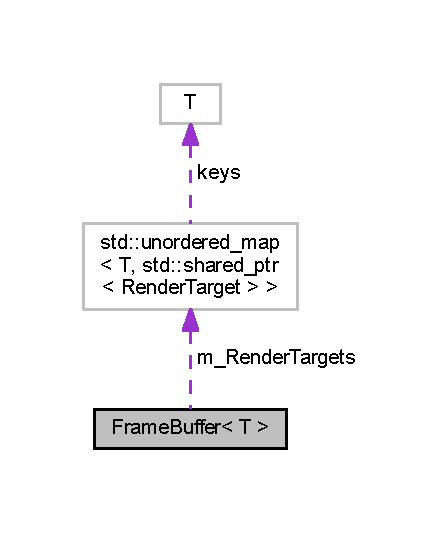
\includegraphics[width=212pt]{class_frame_buffer__coll__graph}
\end{center}
\end{figure}
\subsection*{Public Member Functions}
\begin{DoxyCompactItemize}
\item 
{\bfseries Frame\+Buffer} (int width, int height, bool Depth\+Attachment)\hypertarget{class_frame_buffer_ab7b122bbfc713a58e3d54e5b7474af56}{}\label{class_frame_buffer_ab7b122bbfc713a58e3d54e5b7474af56}

\item 
bool {\bfseries add\+Render\+Target} (T name, int internalformat, int format, int magfilter, int minfilter, bool mipmaps, G\+Luint target=G\+L\+\_\+\+T\+E\+X\+T\+U\+R\+E\+\_\+2D)\hypertarget{class_frame_buffer_ab09573b43ca1906bb3c106f4a9ea7078}{}\label{class_frame_buffer_ab09573b43ca1906bb3c106f4a9ea7078}

\item 
bool {\bfseries Finish\+Frame\+Buffer} ()\hypertarget{class_frame_buffer_ade95eb0f5e2c9112727fd5fcd39e7f98}{}\label{class_frame_buffer_ade95eb0f5e2c9112727fd5fcd39e7f98}

\item 
bool {\bfseries add\+Depth\+Attachment} ()\hypertarget{class_frame_buffer_a10bb6b1df517a12113e37bf913d4f78a}{}\label{class_frame_buffer_a10bb6b1df517a12113e37bf913d4f78a}

\item 
void {\bfseries bind\+Framebuffer} ()\hypertarget{class_frame_buffer_ab8d75432d798f90e01e48f1c8b12cbd2}{}\label{class_frame_buffer_ab8d75432d798f90e01e48f1c8b12cbd2}

\item 
void {\bfseries unbind\+Framebuffer} ()\hypertarget{class_frame_buffer_a28daa4e95495388f1d58ba72cc6b3116}{}\label{class_frame_buffer_a28daa4e95495388f1d58ba72cc6b3116}

\item 
void {\bfseries set\+Viewport} ()\hypertarget{class_frame_buffer_a38d76aa81993cb1bcf28b811ccb7e97e}{}\label{class_frame_buffer_a38d76aa81993cb1bcf28b811ccb7e97e}

\item 
void {\bfseries clear\+Buffer} (int masks)\hypertarget{class_frame_buffer_a9678f75bff552a860451aec9aa268b80}{}\label{class_frame_buffer_a9678f75bff552a860451aec9aa268b80}

\item 
void {\bfseries Update\+Mip\+Maps} ()\hypertarget{class_frame_buffer_ae547f88e0e9081bfd4e8c2cc98ca3198}{}\label{class_frame_buffer_ae547f88e0e9081bfd4e8c2cc98ca3198}

\item 
void {\bfseries set\+To\+Read} ()\hypertarget{class_frame_buffer_aab0e90a873662766c8aeb7d034bf981c}{}\label{class_frame_buffer_aab0e90a873662766c8aeb7d034bf981c}

\item 
void {\bfseries set\+To\+Draw} ()\hypertarget{class_frame_buffer_a7fc09c39eb24e6cadc57b006dd6af0cc}{}\label{class_frame_buffer_a7fc09c39eb24e6cadc57b006dd6af0cc}

\item 
bool {\bfseries check\+Framebuffer} ()\hypertarget{class_frame_buffer_a76d5ef51d24805dd4c2de33dcc598b75}{}\label{class_frame_buffer_a76d5ef51d24805dd4c2de33dcc598b75}

\item 
bool {\bfseries Destroy} ()\hypertarget{class_frame_buffer_afedd4359e85b3588fa11656b9dbade69}{}\label{class_frame_buffer_afedd4359e85b3588fa11656b9dbade69}

\item 
G\+Luint {\bfseries get\+Render\+Target\+Handler} (T name)\hypertarget{class_frame_buffer_aa66d88e11d16a6e505878acca41f872c}{}\label{class_frame_buffer_aa66d88e11d16a6e505878acca41f872c}

\end{DoxyCompactItemize}
\subsection*{Data Fields}
\begin{DoxyCompactItemize}
\item 
std\+::unordered\+\_\+map$<$ T, std\+::shared\+\_\+ptr$<$ \hyperlink{class_render_target}{Render\+Target} $>$ $>$ {\bfseries m\+\_\+\+Render\+Targets}\hypertarget{class_frame_buffer_a7c5cdda0f659fba287d1a5b3d09de387}{}\label{class_frame_buffer_a7c5cdda0f659fba287d1a5b3d09de387}

\item 
int {\bfseries m\+\_\+\+Render\+Target\+Count}\hypertarget{class_frame_buffer_a01b5ec507b23c7b821675308391fc9df}{}\label{class_frame_buffer_a01b5ec507b23c7b821675308391fc9df}

\item 
int {\bfseries M\+A\+X\+\_\+\+R\+E\+N\+D\+E\+R\+\_\+\+T\+A\+R\+G\+E\+TS}\hypertarget{class_frame_buffer_a5b334773e9a54ade675e1b538706eae8}{}\label{class_frame_buffer_a5b334773e9a54ade675e1b538706eae8}

\item 
int {\bfseries W\+I\+D\+TH}\hypertarget{class_frame_buffer_a11fe0a9c9c4f35abd66a2c77e1c740f9}{}\label{class_frame_buffer_a11fe0a9c9c4f35abd66a2c77e1c740f9}

\item 
int {\bfseries H\+E\+I\+G\+HT}\hypertarget{class_frame_buffer_ab85b82233910477a28c1ca8f69dbe555}{}\label{class_frame_buffer_ab85b82233910477a28c1ca8f69dbe555}

\item 
G\+Luint {\bfseries m\+\_\+\+Framebuffer\+Handler}\hypertarget{class_frame_buffer_a16bcb5f0c8a1064dd075b89965b79863}{}\label{class_frame_buffer_a16bcb5f0c8a1064dd075b89965b79863}

\item 
G\+Luint {\bfseries m\+\_\+\+Depth\+Texture\+Target}\hypertarget{class_frame_buffer_a49198d665734401aa6b28860fc9442e8}{}\label{class_frame_buffer_a49198d665734401aa6b28860fc9442e8}

\item 
bool {\bfseries is\+Depth\+Attachment}\hypertarget{class_frame_buffer_a065cf8faab04276cb7e6a4cd004512d1}{}\label{class_frame_buffer_a065cf8faab04276cb7e6a4cd004512d1}

\end{DoxyCompactItemize}


\subsection{Detailed Description}
\subsubsection*{template$<$typename T$>$\\*
class Frame\+Buffer$<$ T $>$}



Definition at line 11 of file Frame\+Buffer.\+h.


\hypertarget{struct_m_d5_animation_1_1_frame_data}{}\section{M\+D5\+Animation\+:\+:Frame\+Data Struct Reference}
\label{struct_m_d5_animation_1_1_frame_data}\index{M\+D5\+Animation\+::\+Frame\+Data@{M\+D5\+Animation\+::\+Frame\+Data}}


Collaboration diagram for M\+D5\+Animation\+:\+:Frame\+Data\+:
\nopagebreak
\begin{figure}[H]
\begin{center}
\leavevmode
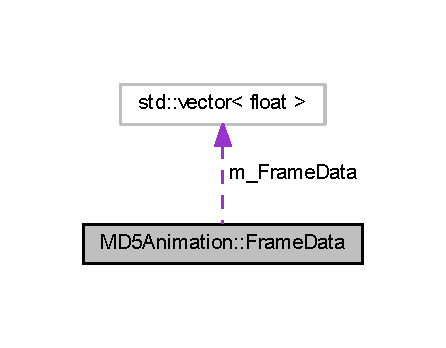
\includegraphics[width=214pt]{struct_m_d5_animation_1_1_frame_data__coll__graph}
\end{center}
\end{figure}
\subsection*{Data Fields}
\begin{DoxyCompactItemize}
\item 
int {\bfseries m\+\_\+i\+Frame\+ID}\hypertarget{struct_m_d5_animation_1_1_frame_data_aabde95278d7c492302eff0588d4df8ae}{}\label{struct_m_d5_animation_1_1_frame_data_aabde95278d7c492302eff0588d4df8ae}

\item 
std\+::vector$<$ float $>$ {\bfseries m\+\_\+\+Frame\+Data}\hypertarget{struct_m_d5_animation_1_1_frame_data_aae7ffea26bf8b0ea133a0ed2e04f164f}{}\label{struct_m_d5_animation_1_1_frame_data_aae7ffea26bf8b0ea133a0ed2e04f164f}

\end{DoxyCompactItemize}


\subsection{Detailed Description}


Definition at line 48 of file M\+D5\+\_\+\+Anim.\+h.


\hypertarget{struct_m_d5_animation_1_1_frame_skeleton}{}\section{M\+D5\+Animation\+:\+:Frame\+Skeleton Struct Reference}
\label{struct_m_d5_animation_1_1_frame_skeleton}\index{M\+D5\+Animation\+::\+Frame\+Skeleton@{M\+D5\+Animation\+::\+Frame\+Skeleton}}


Collaboration diagram for M\+D5\+Animation\+:\+:Frame\+Skeleton\+:
\nopagebreak
\begin{figure}[H]
\begin{center}
\leavevmode
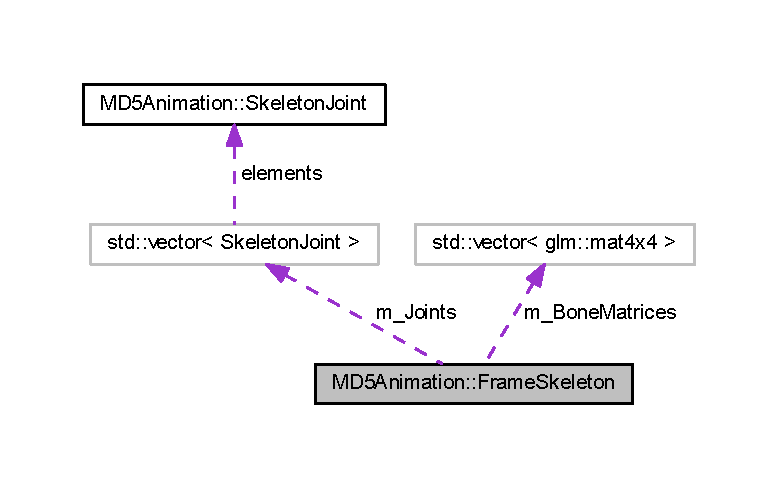
\includegraphics[width=350pt]{struct_m_d5_animation_1_1_frame_skeleton__coll__graph}
\end{center}
\end{figure}
\subsection*{Data Fields}
\begin{DoxyCompactItemize}
\item 
Skeleton\+Matrix\+List {\bfseries m\+\_\+\+Bone\+Matrices}\hypertarget{struct_m_d5_animation_1_1_frame_skeleton_a614fe6f4ce905af6da3cb6f6f3a7a5cd}{}\label{struct_m_d5_animation_1_1_frame_skeleton_a614fe6f4ce905af6da3cb6f6f3a7a5cd}

\item 
Skeleton\+Joint\+List {\bfseries m\+\_\+\+Joints}\hypertarget{struct_m_d5_animation_1_1_frame_skeleton_a65ce440d467eaae6c3cbbf94eb1d91b9}{}\label{struct_m_d5_animation_1_1_frame_skeleton_a65ce440d467eaae6c3cbbf94eb1d91b9}

\end{DoxyCompactItemize}


\subsection{Detailed Description}


Definition at line 76 of file M\+D5\+\_\+\+Anim.\+h.


\hypertarget{class_open_g_l_helpers_1_1_full_screen_quad}{}\section{Open\+G\+L\+Helpers\+:\+:Full\+Screen\+Quad Class Reference}
\label{class_open_g_l_helpers_1_1_full_screen_quad}\index{Open\+G\+L\+Helpers\+::\+Full\+Screen\+Quad@{Open\+G\+L\+Helpers\+::\+Full\+Screen\+Quad}}
\subsection*{Public Member Functions}
\begin{DoxyCompactItemize}
\item 
void {\bfseries Render} ()\hypertarget{class_open_g_l_helpers_1_1_full_screen_quad_a2758c7738ae496e95573fa7ee5e7fdc7}{}\label{class_open_g_l_helpers_1_1_full_screen_quad_a2758c7738ae496e95573fa7ee5e7fdc7}

\end{DoxyCompactItemize}
\subsection*{Private Attributes}
\begin{DoxyCompactItemize}
\item 
G\+Luint {\bfseries quad\+V\+AO} = 0\hypertarget{class_open_g_l_helpers_1_1_full_screen_quad_a770f3df38a60f16641e4917b1db747d8}{}\label{class_open_g_l_helpers_1_1_full_screen_quad_a770f3df38a60f16641e4917b1db747d8}

\item 
G\+Luint {\bfseries quad\+V\+BO} = 0\hypertarget{class_open_g_l_helpers_1_1_full_screen_quad_a2079668e16561c8c7088912bc11d9852}{}\label{class_open_g_l_helpers_1_1_full_screen_quad_a2079668e16561c8c7088912bc11d9852}

\end{DoxyCompactItemize}


\subsection{Detailed Description}


Definition at line 5 of file Full\+Screen\+Quad.\+h.


\hypertarget{classgl_cache}{}\section{gl\+Cache Class Reference}
\label{classgl_cache}\index{gl\+Cache@{gl\+Cache}}
\subsection*{Static Public Member Functions}
\begin{DoxyCompactItemize}
\item 
static void {\bfseries gl\+Use\+Program} (G\+Luint program)\hypertarget{classgl_cache_a7788c5bc421f4fffb0c558e9613f8f14}{}\label{classgl_cache_a7788c5bc421f4fffb0c558e9613f8f14}

\item 
static void {\bfseries gl\+Cull\+Face} (G\+Lenum mode)\hypertarget{classgl_cache_ab8013e9005e6cb79a2754aa512de4dc9}{}\label{classgl_cache_ab8013e9005e6cb79a2754aa512de4dc9}

\item 
static void {\bfseries gl\+Enable} (G\+Lenum cap)\hypertarget{classgl_cache_a1388678233c21888b944fe27a3133928}{}\label{classgl_cache_a1388678233c21888b944fe27a3133928}

\item 
static void {\bfseries gl\+Draw\+Elements} (G\+Lenum mode, G\+Lsizei count, G\+Lenum type, const G\+Lvoid $\ast$indices)\hypertarget{classgl_cache_a1e84f8e987b546a678be7e2fa502af59}{}\label{classgl_cache_a1e84f8e987b546a678be7e2fa502af59}

\item 
static void {\bfseries gl\+Draw\+Arrays} (G\+Lenum mode, G\+Lint first, G\+Lsizei count)\hypertarget{classgl_cache_ae108a3ad73abd1e44ef465c291ec4830}{}\label{classgl_cache_ae108a3ad73abd1e44ef465c291ec4830}

\end{DoxyCompactItemize}
\subsection*{Static Public Attributes}
\begin{DoxyCompactItemize}
\item 
static G\+Luint {\bfseries Shader\+Id} = 0\hypertarget{classgl_cache_aff46755b94de4b4abaf376eeca078c50}{}\label{classgl_cache_aff46755b94de4b4abaf376eeca078c50}

\item 
static G\+Lenum {\bfseries Cull\+Face\+Mode} = 0\hypertarget{classgl_cache_a59fe6f35f12e7cdc8e99d559060493ca}{}\label{classgl_cache_a59fe6f35f12e7cdc8e99d559060493ca}

\item 
static unsigned {\bfseries Draw\+Calls} = 0\hypertarget{classgl_cache_aa8fd4d4ed98423ba342d3969a8082807}{}\label{classgl_cache_aa8fd4d4ed98423ba342d3969a8082807}

\end{DoxyCompactItemize}


\subsection{Detailed Description}


Definition at line 5 of file Gl\+Cache.\+h.


\hypertarget{class_g_p_u}{}\section{G\+PU Class Reference}
\label{class_g_p_u}\index{G\+PU@{G\+PU}}


Collaboration diagram for G\+PU\+:
\nopagebreak
\begin{figure}[H]
\begin{center}
\leavevmode
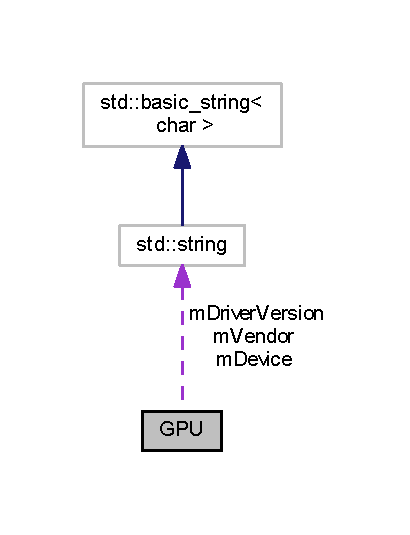
\includegraphics[width=197pt]{class_g_p_u__coll__graph}
\end{center}
\end{figure}
\subsection*{Public Member Functions}
\begin{DoxyCompactItemize}
\item 
std\+::string {\bfseries get\+Driver\+Version} ()\hypertarget{class_g_p_u_ae92cd8553e3017952372f0d9a0a0a6aa}{}\label{class_g_p_u_ae92cd8553e3017952372f0d9a0a0a6aa}

\item 
std\+::string {\bfseries get\+Vendor} ()\hypertarget{class_g_p_u_a7f302d02f8828a87659706ac6ea7e2ce}{}\label{class_g_p_u_a7f302d02f8828a87659706ac6ea7e2ce}

\item 
std\+::string {\bfseries get\+Device} ()\hypertarget{class_g_p_u_ac4814898ff4886efbb19c1136c438e9b}{}\label{class_g_p_u_ac4814898ff4886efbb19c1136c438e9b}

\item 
size\+\_\+t {\bfseries get\+Available\+Memory} ()\hypertarget{class_g_p_u_a49b8fa7e391cf16dbae0f9b17841eff3}{}\label{class_g_p_u_a49b8fa7e391cf16dbae0f9b17841eff3}

\item 
size\+\_\+t {\bfseries get\+Total\+Memory} ()\hypertarget{class_g_p_u_acab8ea6309c537472ff8eceb58e4bcc0}{}\label{class_g_p_u_acab8ea6309c537472ff8eceb58e4bcc0}

\end{DoxyCompactItemize}
\subsection*{Private Attributes}
\begin{DoxyCompactItemize}
\item 
std\+::string {\bfseries m\+Vendor}\hypertarget{class_g_p_u_a175c63d0f5ef908a0e20b7fef32746a3}{}\label{class_g_p_u_a175c63d0f5ef908a0e20b7fef32746a3}

\item 
std\+::string {\bfseries m\+Driver\+Version}\hypertarget{class_g_p_u_ac6751bd68c6dca89bd8ef5a4caf88aa6}{}\label{class_g_p_u_ac6751bd68c6dca89bd8ef5a4caf88aa6}

\item 
std\+::string {\bfseries m\+Device}\hypertarget{class_g_p_u_ae090ffd3784da047f027ec0ad804b59e}{}\label{class_g_p_u_ae090ffd3784da047f027ec0ad804b59e}

\end{DoxyCompactItemize}


\subsection{Detailed Description}


Definition at line 5 of file G\+P\+U.\+hpp.


\hypertarget{class_grass}{}\section{Grass Class Reference}
\label{class_grass}\index{Grass@{Grass}}


Collaboration diagram for Grass\+:
\nopagebreak
\begin{figure}[H]
\begin{center}
\leavevmode
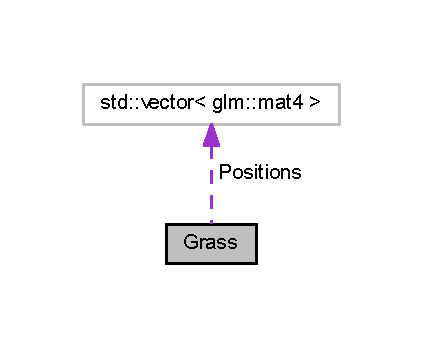
\includegraphics[width=203pt]{class_grass__coll__graph}
\end{center}
\end{figure}
\subsection*{Public Member Functions}
\begin{DoxyCompactItemize}
\item 
{\bfseries Grass} (const char $\ast$path, std\+::vector$<$ glm\+::vec3 $>$ grass\+Pos)\hypertarget{class_grass_abc975681174b5f67d3116c5bdbec65c0}{}\label{class_grass_abc975681174b5f67d3116c5bdbec65c0}

\item 
void {\bfseries Render} (\hyperlink{class_shader}{Shader} $\ast$shader)\hypertarget{class_grass_a5d3aa3ab5ad807f3cdd9b655da53f3b7}{}\label{class_grass_a5d3aa3ab5ad807f3cdd9b655da53f3b7}

\end{DoxyCompactItemize}
\subsection*{Private Attributes}
\begin{DoxyCompactItemize}
\item 
G\+Luint {\bfseries V\+BO}\hypertarget{class_grass_a94546b98c58f2a74a91ad59f73036f8b}{}\label{class_grass_a94546b98c58f2a74a91ad59f73036f8b}

\item 
G\+Luint {\bfseries E\+BO}\hypertarget{class_grass_a054fd25dde0d19e2b272f8aa611e7b3e}{}\label{class_grass_a054fd25dde0d19e2b272f8aa611e7b3e}

\item 
G\+Luint {\bfseries V\+AO}\hypertarget{class_grass_a35f97e4d959542776ba90ad2e0908260}{}\label{class_grass_a35f97e4d959542776ba90ad2e0908260}

\item 
G\+Luint {\bfseries grass\+Texture}\hypertarget{class_grass_a026bbcbfbb49b9557801943723cb01be}{}\label{class_grass_a026bbcbfbb49b9557801943723cb01be}

\item 
std\+::vector$<$ glm\+::mat4 $>$ {\bfseries Positions}\hypertarget{class_grass_a816ecede6a8d916dbeb4e446de98c5a5}{}\label{class_grass_a816ecede6a8d916dbeb4e446de98c5a5}

\item 
int {\bfseries amount}\hypertarget{class_grass_a129256ec74373edd2d18654102ade669}{}\label{class_grass_a129256ec74373edd2d18654102ade669}

\item 
G\+Lfloat {\bfseries Grass\+Vertices} \mbox{[}64\mbox{]}
\item 
G\+Luint {\bfseries Grass\+Indices} \mbox{[}12\mbox{]}
\end{DoxyCompactItemize}


\subsection{Detailed Description}
========= Copyright Survtech, All rights reserved. ============//

Purpose\+: 

 

Definition at line 18 of file Grass.\+h.



\subsection{Field Documentation}
\index{Grass@{Grass}!Grass\+Indices@{Grass\+Indices}}
\index{Grass\+Indices@{Grass\+Indices}!Grass@{Grass}}
\subsubsection[{\texorpdfstring{Grass\+Indices}{GrassIndices}}]{\setlength{\rightskip}{0pt plus 5cm}G\+Luint Grass\+::\+Grass\+Indices\mbox{[}12\mbox{]}\hspace{0.3cm}{\ttfamily [private]}}\hypertarget{class_grass_a2a7aecffc8204c7b6d268d91f37eea3d}{}\label{class_grass_a2a7aecffc8204c7b6d268d91f37eea3d}
{\bfseries Initial value\+:}
\begin{DoxyCode}
=
    \{
        0, 1, 3,
        1, 2, 3,
        4, 5, 7,
        5, 6, 7
    \}
\end{DoxyCode}


Definition at line 133 of file Grass.\+h.

\index{Grass@{Grass}!Grass\+Vertices@{Grass\+Vertices}}
\index{Grass\+Vertices@{Grass\+Vertices}!Grass@{Grass}}
\subsubsection[{\texorpdfstring{Grass\+Vertices}{GrassVertices}}]{\setlength{\rightskip}{0pt plus 5cm}G\+Lfloat Grass\+::\+Grass\+Vertices\mbox{[}64\mbox{]}\hspace{0.3cm}{\ttfamily [private]}}\hypertarget{class_grass_ae23b5fc33245f28237d2232c49adcdca}{}\label{class_grass_ae23b5fc33245f28237d2232c49adcdca}
{\bfseries Initial value\+:}
\begin{DoxyCode}
=
    \{
        0.5f,  0.5f,  0.0f, 0.0f, 0.0f, 0.0, 1.0, 0.0,
        0.5f, -0.5f,  0.0f, 0.0f, 1.0f, 0.0, 1.0, 0.0,
        -0.5f, -0.5f,  0.0f, 1.0f, 1.0f, 0.0, 1.0, 0.0,
        -0.5f,  0.5f,  0.0f, 1.0f, 0.0f, 0.0, 1.0, 0.0,

        0.0f,  0.5f,  0.5f, 1.0f, 0.0f, 0.0, 1.0, 0.0,
        0.0f,  0.5f, -0.5f, 0.0f, 0.0f, 0.0, 1.0, 0.0,
        0.0f, -0.5f, -0.5f, 0.0f, 1.0f, 0.0, 1.0, 0.0,
        0.0f, -0.5f,  0.5f, 1.0f, 1.0f, 0.0, 1.0, 0.0
    \}
\end{DoxyCode}


Definition at line 120 of file Grass.\+h.


\hypertarget{class_g_u_i}{}\section{G\+UI Class Reference}
\label{class_g_u_i}\index{G\+UI@{G\+UI}}


Collaboration diagram for G\+UI\+:
\nopagebreak
\begin{figure}[H]
\begin{center}
\leavevmode
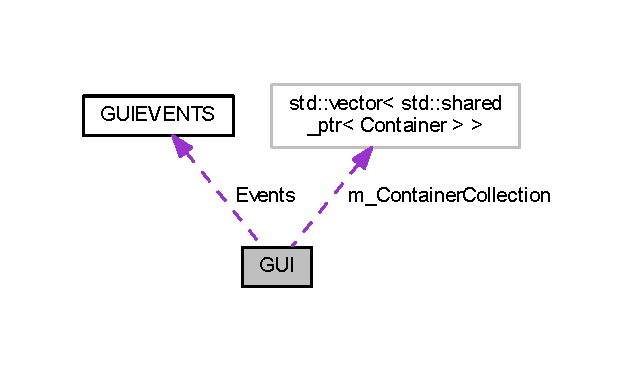
\includegraphics[width=305pt]{class_g_u_i__coll__graph}
\end{center}
\end{figure}
\subsection*{Public Member Functions}
\begin{DoxyCompactItemize}
\item 
{\bfseries G\+UI} (int win\+Width, int win\+Height)\hypertarget{class_g_u_i_a200d23809446a60bf9b9ea4c0ae30c46}{}\label{class_g_u_i_a200d23809446a60bf9b9ea4c0ae30c46}

\item 
void {\bfseries Render} ()\hypertarget{class_g_u_i_a4905ff37be14b83496d098096f5848b6}{}\label{class_g_u_i_a4905ff37be14b83496d098096f5848b6}

\item 
bool {\bfseries Add\+Container} (std\+::shared\+\_\+ptr$<$ \hyperlink{class_container}{Container} $>$ container)\hypertarget{class_g_u_i_a54dfaebb735e37ad855512018039a969}{}\label{class_g_u_i_a54dfaebb735e37ad855512018039a969}

\item 
bool {\bfseries G\+U\+I\+Remove\+Widget} (int Widget\+ID)\hypertarget{class_g_u_i_a6efb59f469126f8629ed5f0acc5138fb}{}\label{class_g_u_i_a6efb59f469126f8629ed5f0acc5138fb}

\item 
void {\bfseries Poll\+Events} (G\+L\+F\+Wwindow $\ast$window)\hypertarget{class_g_u_i_a2afd27aa7203549ebcd97ff4777a683a}{}\label{class_g_u_i_a2afd27aa7203549ebcd97ff4777a683a}

\end{DoxyCompactItemize}
\subsection*{Private Attributes}
\begin{DoxyCompactItemize}
\item 
std\+::vector$<$ std\+::shared\+\_\+ptr$<$ \hyperlink{class_container}{Container} $>$ $>$ {\bfseries m\+\_\+\+Container\+Collection}\hypertarget{class_g_u_i_a35b7b035ba9ffe52e98216cb14cf0108}{}\label{class_g_u_i_a35b7b035ba9ffe52e98216cb14cf0108}

\item 
std\+::shared\+\_\+ptr$<$ \hyperlink{class_shader}{Shader} $>$ {\bfseries m\+\_\+\+Shader}\hypertarget{class_g_u_i_a75e3b7c07e1559e346680326a439fe74}{}\label{class_g_u_i_a75e3b7c07e1559e346680326a439fe74}

\item 
\hyperlink{struct_g_u_i_e_v_e_n_t_s}{G\+U\+I\+E\+V\+E\+N\+TS} {\bfseries Events}\hypertarget{class_g_u_i_aa4806d12dd478a1cacd0a20b59d22298}{}\label{class_g_u_i_aa4806d12dd478a1cacd0a20b59d22298}

\item 
int {\bfseries m\+\_\+\+Window\+Width}\hypertarget{class_g_u_i_a0a5ea53e7f6ce833842c6f6e7735ece3}{}\label{class_g_u_i_a0a5ea53e7f6ce833842c6f6e7735ece3}

\item 
int {\bfseries m\+\_\+\+Window\+Height}\hypertarget{class_g_u_i_a2d95e4f6e7347c11197f2ec1aadf1d92}{}\label{class_g_u_i_a2d95e4f6e7347c11197f2ec1aadf1d92}

\end{DoxyCompactItemize}


\subsection{Detailed Description}


Definition at line 7 of file G\+U\+I.\+h.


\hypertarget{struct_g_u_i_e_v_e_n_t_s}{}\section{G\+U\+I\+E\+V\+E\+N\+TS Struct Reference}
\label{struct_g_u_i_e_v_e_n_t_s}\index{G\+U\+I\+E\+V\+E\+N\+TS@{G\+U\+I\+E\+V\+E\+N\+TS}}
\subsection*{Data Fields}
\begin{DoxyCompactItemize}
\item 
double {\bfseries Mouse\+Position} \mbox{[}2\mbox{]}\hypertarget{struct_g_u_i_e_v_e_n_t_s_a43970005b3aad1aa4c02e0d4043d0cee}{}\label{struct_g_u_i_e_v_e_n_t_s_a43970005b3aad1aa4c02e0d4043d0cee}

\item 
bool {\bfseries Key\+Pressed} \mbox{[}256\mbox{]}\hypertarget{struct_g_u_i_e_v_e_n_t_s_a9ce1ca9dd931e80ddb093a561bb607d9}{}\label{struct_g_u_i_e_v_e_n_t_s_a9ce1ca9dd931e80ddb093a561bb607d9}

\item 
bool {\bfseries Right\+Click\+Was\+Pressed}\hypertarget{struct_g_u_i_e_v_e_n_t_s_a69e9249aae5d7d2333e1882fdac40615}{}\label{struct_g_u_i_e_v_e_n_t_s_a69e9249aae5d7d2333e1882fdac40615}

\item 
bool {\bfseries Left\+Click\+Was\+Pressed}\hypertarget{struct_g_u_i_e_v_e_n_t_s_a61e98cb8bce7c193d836acd09e933603}{}\label{struct_g_u_i_e_v_e_n_t_s_a61e98cb8bce7c193d836acd09e933603}

\end{DoxyCompactItemize}


\subsection{Detailed Description}


Definition at line 169 of file Types.\+h.


\hypertarget{class_i_o_1_1_image_1_1_image}{}\section{IO\+:\+:Image\+:\+:Image Class Reference}
\label{class_i_o_1_1_image_1_1_image}\index{I\+O\+::\+Image\+::\+Image@{I\+O\+::\+Image\+::\+Image}}


Collaboration diagram for IO\+:\+:Image\+:\+:Image\+:
\nopagebreak
\begin{figure}[H]
\begin{center}
\leavevmode
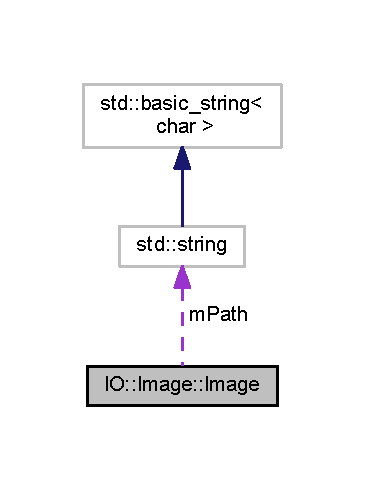
\includegraphics[width=175pt]{class_i_o_1_1_image_1_1_image__coll__graph}
\end{center}
\end{figure}
\subsection*{Public Types}
\begin{DoxyCompactItemize}
\item 
typedef std\+::shared\+\_\+ptr$<$ \hyperlink{class_i_o_1_1_image_1_1_image}{I\+O\+::\+Image\+::\+Image} $>$ {\bfseries Image\+\_\+ptr}\hypertarget{class_i_o_1_1_image_1_1_image_a2278b8aad75cd25274b860851cfa3327}{}\label{class_i_o_1_1_image_1_1_image_a2278b8aad75cd25274b860851cfa3327}

\end{DoxyCompactItemize}
\subsection*{Public Member Functions}
\begin{DoxyCompactItemize}
\item 
void {\bfseries Load\+File} (const char $\ast$path, unsigned char $\ast$\&data, int $\ast$outwidth, int $\ast$outheight, int $\ast$outchannels)\hypertarget{class_i_o_1_1_image_1_1_image_a05f99148e9bef11345479f217904f67d}{}\label{class_i_o_1_1_image_1_1_image_a05f99148e9bef11345479f217904f67d}

\item 
void {\bfseries Load\+File} (const char $\ast$path)\hypertarget{class_i_o_1_1_image_1_1_image_a5f5bcdb4e1a2e0931e26b568a28a2f5d}{}\label{class_i_o_1_1_image_1_1_image_a5f5bcdb4e1a2e0931e26b568a28a2f5d}

\item 
void {\bfseries Load} ()\hypertarget{class_i_o_1_1_image_1_1_image_a9f1a3f64b2ef92c54db583194a9f8091}{}\label{class_i_o_1_1_image_1_1_image_a9f1a3f64b2ef92c54db583194a9f8091}

\item 
void {\bfseries get\+Size\+P\+NG} (const char $\ast$p, int $\ast$w, int $\ast$h, int $\ast$c)\hypertarget{class_i_o_1_1_image_1_1_image_a1541631a67ad6872fa5c133b7a49e4af}{}\label{class_i_o_1_1_image_1_1_image_a1541631a67ad6872fa5c133b7a49e4af}

\item 
void {\bfseries get\+Size\+B\+MP} (const char $\ast$p, int $\ast$w, int $\ast$h)\hypertarget{class_i_o_1_1_image_1_1_image_a69b4e9d76b76809b4fdf18dd2a0a716b}{}\label{class_i_o_1_1_image_1_1_image_a69b4e9d76b76809b4fdf18dd2a0a716b}

\item 
void {\bfseries get\+Size\+T\+GA} (const char $\ast$p, int $\ast$w, int $\ast$h)\hypertarget{class_i_o_1_1_image_1_1_image_abe305d4223885aa9b8da93584ca94f2c}{}\label{class_i_o_1_1_image_1_1_image_abe305d4223885aa9b8da93584ca94f2c}

\item 
void {\bfseries get\+Size\+D\+DS} (const char $\ast$p, int $\ast$w, int $\ast$h)\hypertarget{class_i_o_1_1_image_1_1_image_a8a88ebfab83bb7625b2a9e0d363525d1}{}\label{class_i_o_1_1_image_1_1_image_a8a88ebfab83bb7625b2a9e0d363525d1}

\item 
bool {\bfseries is\+Loaded} ()\hypertarget{class_i_o_1_1_image_1_1_image_a58bb5e5fd453bab092bc37e2cb9b67e9}{}\label{class_i_o_1_1_image_1_1_image_a58bb5e5fd453bab092bc37e2cb9b67e9}

\item 
void {\bfseries on\+Load} (std\+::function$<$ void()$>$ f)\hypertarget{class_i_o_1_1_image_1_1_image_af7422a0799029301e1788a1feab10998}{}\label{class_i_o_1_1_image_1_1_image_af7422a0799029301e1788a1feab10998}

\item 
unsigned char $\ast$ {\bfseries get\+Data} ()\hypertarget{class_i_o_1_1_image_1_1_image_ac40aed74c1c40aedcec355443164b303}{}\label{class_i_o_1_1_image_1_1_image_ac40aed74c1c40aedcec355443164b303}

\end{DoxyCompactItemize}
\subsection*{Data Fields}
\begin{DoxyCompactItemize}
\item 
std\+::function$<$ void()$>$ {\bfseries On\+Load} = nullptr\hypertarget{class_i_o_1_1_image_1_1_image_a179048eccc6df5d42d06106b9a9f4e80}{}\label{class_i_o_1_1_image_1_1_image_a179048eccc6df5d42d06106b9a9f4e80}

\item 
std\+::shared\+\_\+ptr$<$ std\+::thread $>$ {\bfseries th1}\hypertarget{class_i_o_1_1_image_1_1_image_a4e40dcbffacded80f3b077e43a24aec1}{}\label{class_i_o_1_1_image_1_1_image_a4e40dcbffacded80f3b077e43a24aec1}

\end{DoxyCompactItemize}
\subsection*{Private Attributes}
\begin{DoxyCompactItemize}
\item 
bool {\bfseries m\+Loaded} = false\hypertarget{class_i_o_1_1_image_1_1_image_ae7de8af3717796c8c86c8d1cb31ed2a2}{}\label{class_i_o_1_1_image_1_1_image_ae7de8af3717796c8c86c8d1cb31ed2a2}

\item 
unsigned char $\ast$ {\bfseries m\+Data} = nullptr\hypertarget{class_i_o_1_1_image_1_1_image_a1be4ab27ddce7814942bbccd097bc9b6}{}\label{class_i_o_1_1_image_1_1_image_a1be4ab27ddce7814942bbccd097bc9b6}

\item 
std\+::string {\bfseries m\+Path} = \char`\"{}\char`\"{}\hypertarget{class_i_o_1_1_image_1_1_image_a597d7b71a0ceb9c95bf6466d23c7c475}{}\label{class_i_o_1_1_image_1_1_image_a597d7b71a0ceb9c95bf6466d23c7c475}

\item 
int {\bfseries m\+Width} = 0\hypertarget{class_i_o_1_1_image_1_1_image_a2e11c19dab536fa7575be8930d98676a}{}\label{class_i_o_1_1_image_1_1_image_a2e11c19dab536fa7575be8930d98676a}

\item 
int {\bfseries m\+Height} = 0\hypertarget{class_i_o_1_1_image_1_1_image_a8805b40269a0ea9014448eee65406eed}{}\label{class_i_o_1_1_image_1_1_image_a8805b40269a0ea9014448eee65406eed}

\end{DoxyCompactItemize}


\subsection{Detailed Description}


Definition at line 16 of file Image.\+hpp.


\hypertarget{class_thread_1_1_job}{}\section{Thread\+:\+:Job$<$ T $>$ Class Template Reference}
\label{class_thread_1_1_job}\index{Thread\+::\+Job$<$ T $>$@{Thread\+::\+Job$<$ T $>$}}


Collaboration diagram for Thread\+:\+:Job$<$ T $>$\+:
\nopagebreak
\begin{figure}[H]
\begin{center}
\leavevmode
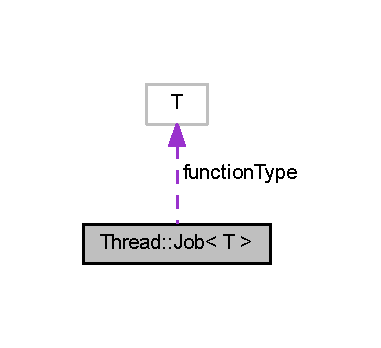
\includegraphics[width=183pt]{class_thread_1_1_job__coll__graph}
\end{center}
\end{figure}
\subsection*{Public Member Functions}
\begin{DoxyCompactItemize}
\item 
int {\bfseries Begin} ()\hypertarget{class_thread_1_1_job_a7be347617e4125390298491976176f4d}{}\label{class_thread_1_1_job_a7be347617e4125390298491976176f4d}

\item 
int {\bfseries Finish} ()\hypertarget{class_thread_1_1_job_aabf96ee68a4917da6cc7dec07f976502}{}\label{class_thread_1_1_job_aabf96ee68a4917da6cc7dec07f976502}

\end{DoxyCompactItemize}
\subsection*{Private Attributes}
\begin{DoxyCompactItemize}
\item 
std\+::shared\+\_\+ptr$<$ Thread $>$ {\bfseries m\+Thread}\hypertarget{class_thread_1_1_job_a7507a46d46adedc70d4c579f12012a25}{}\label{class_thread_1_1_job_a7507a46d46adedc70d4c579f12012a25}

\item 
std\+::function$<$ T $>$ {\bfseries m\+Function}\hypertarget{class_thread_1_1_job_a9d8b19e5e3b47e790266a0e79eee56e7}{}\label{class_thread_1_1_job_a9d8b19e5e3b47e790266a0e79eee56e7}

\item 
T {\bfseries function\+Type}\hypertarget{class_thread_1_1_job_adb49d85ea08e42c1e2f9b10d9823ede7}{}\label{class_thread_1_1_job_adb49d85ea08e42c1e2f9b10d9823ede7}

\end{DoxyCompactItemize}


\subsection{Detailed Description}
\subsubsection*{template$<$typename T$>$\\*
class Thread\+::\+Job$<$ T $>$}



Definition at line 8 of file Job.\+h.


\hypertarget{struct_m_d5_model_1_1_joint}{}\section{M\+D5\+Model\+:\+:Joint Struct Reference}
\label{struct_m_d5_model_1_1_joint}\index{M\+D5\+Model\+::\+Joint@{M\+D5\+Model\+::\+Joint}}


Collaboration diagram for M\+D5\+Model\+:\+:Joint\+:
\nopagebreak
\begin{figure}[H]
\begin{center}
\leavevmode
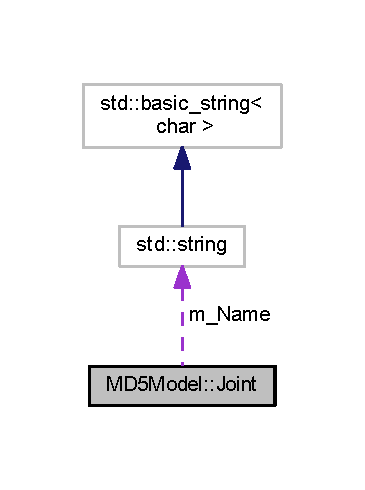
\includegraphics[width=175pt]{struct_m_d5_model_1_1_joint__coll__graph}
\end{center}
\end{figure}
\subsection*{Data Fields}
\begin{DoxyCompactItemize}
\item 
std\+::string {\bfseries m\+\_\+\+Name}\hypertarget{struct_m_d5_model_1_1_joint_a87fc950b11a52a0f5c3ac5ef8ec554ac}{}\label{struct_m_d5_model_1_1_joint_a87fc950b11a52a0f5c3ac5ef8ec554ac}

\item 
int {\bfseries m\+\_\+\+Parent\+ID}\hypertarget{struct_m_d5_model_1_1_joint_a386ca25e937f6341eb8a2afd1d2165e8}{}\label{struct_m_d5_model_1_1_joint_a386ca25e937f6341eb8a2afd1d2165e8}

\item 
glm\+::vec3 {\bfseries m\+\_\+\+Pos}\hypertarget{struct_m_d5_model_1_1_joint_ad0858a102b54299e5fe8ad942acffea0}{}\label{struct_m_d5_model_1_1_joint_ad0858a102b54299e5fe8ad942acffea0}

\item 
glm\+::quat {\bfseries m\+\_\+\+Orient}\hypertarget{struct_m_d5_model_1_1_joint_a9fbf36372259c5d1c877b06c991c279b}{}\label{struct_m_d5_model_1_1_joint_a9fbf36372259c5d1c877b06c991c279b}

\end{DoxyCompactItemize}


\subsection{Detailed Description}


Definition at line 66 of file M\+D5\+\_\+\+Model.\+h.


\hypertarget{struct_m_d5_model_1_1_joint_draw_info}{}\section{M\+D5\+Model\+:\+:Joint\+Draw\+Info Struct Reference}
\label{struct_m_d5_model_1_1_joint_draw_info}\index{M\+D5\+Model\+::\+Joint\+Draw\+Info@{M\+D5\+Model\+::\+Joint\+Draw\+Info}}


Collaboration diagram for M\+D5\+Model\+:\+:Joint\+Draw\+Info\+:
\nopagebreak
\begin{figure}[H]
\begin{center}
\leavevmode
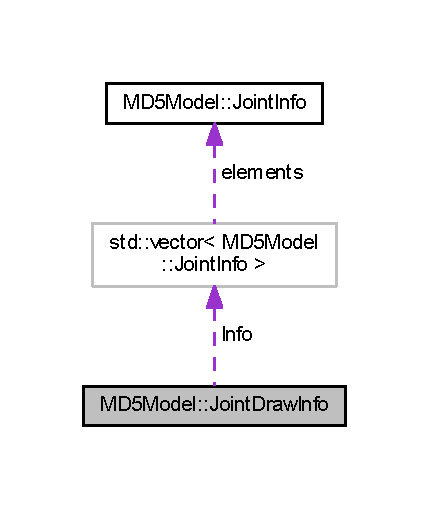
\includegraphics[width=206pt]{struct_m_d5_model_1_1_joint_draw_info__coll__graph}
\end{center}
\end{figure}
\subsection*{Data Fields}
\begin{DoxyCompactItemize}
\item 
G\+Luint {\bfseries V\+AO}\hypertarget{struct_m_d5_model_1_1_joint_draw_info_accb2b4c2c2fbf73f93d8109d2a749efb}{}\label{struct_m_d5_model_1_1_joint_draw_info_accb2b4c2c2fbf73f93d8109d2a749efb}

\item 
G\+Luint {\bfseries V\+BO}\hypertarget{struct_m_d5_model_1_1_joint_draw_info_aa5f0b55afe49b644ab90888278432ff6}{}\label{struct_m_d5_model_1_1_joint_draw_info_aa5f0b55afe49b644ab90888278432ff6}

\item 
std\+::vector$<$ \hyperlink{struct_m_d5_model_1_1_joint_info}{Joint\+Info} $>$ {\bfseries Info}\hypertarget{struct_m_d5_model_1_1_joint_draw_info_acc6911d2241afb5a71d9f040e51a3357}{}\label{struct_m_d5_model_1_1_joint_draw_info_acc6911d2241afb5a71d9f040e51a3357}

\end{DoxyCompactItemize}


\subsection{Detailed Description}


Definition at line 170 of file M\+D5\+\_\+\+Model.\+h.


\hypertarget{struct_m_d5_animation_1_1_joint_info}{}\section{M\+D5\+Animation\+:\+:Joint\+Info Struct Reference}
\label{struct_m_d5_animation_1_1_joint_info}\index{M\+D5\+Animation\+::\+Joint\+Info@{M\+D5\+Animation\+::\+Joint\+Info}}


Collaboration diagram for M\+D5\+Animation\+:\+:Joint\+Info\+:
\nopagebreak
\begin{figure}[H]
\begin{center}
\leavevmode
\includegraphics[width=202pt]{struct_m_d5_animation_1_1_joint_info__coll__graph}
\end{center}
\end{figure}
\subsection*{Data Fields}
\begin{DoxyCompactItemize}
\item 
std\+::string {\bfseries m\+\_\+\+Name}\hypertarget{struct_m_d5_animation_1_1_joint_info_a96689c5c43ab55c4ea81ad9cf45a71b2}{}\label{struct_m_d5_animation_1_1_joint_info_a96689c5c43ab55c4ea81ad9cf45a71b2}

\item 
int {\bfseries m\+\_\+\+Parent\+ID}\hypertarget{struct_m_d5_animation_1_1_joint_info_aa6e4fd111213167c87341bfb04a7bb8b}{}\label{struct_m_d5_animation_1_1_joint_info_aa6e4fd111213167c87341bfb04a7bb8b}

\item 
int {\bfseries m\+\_\+\+Flags}\hypertarget{struct_m_d5_animation_1_1_joint_info_af17256b6479a8888116cc8e62b3844d0}{}\label{struct_m_d5_animation_1_1_joint_info_af17256b6479a8888116cc8e62b3844d0}

\item 
int {\bfseries m\+\_\+\+Start\+Index}\hypertarget{struct_m_d5_animation_1_1_joint_info_af95e9e7800f0a4dafe62b86cf60efb46}{}\label{struct_m_d5_animation_1_1_joint_info_af95e9e7800f0a4dafe62b86cf60efb46}

\end{DoxyCompactItemize}


\subsection{Detailed Description}


Definition at line 25 of file M\+D5\+\_\+\+Anim.\+h.


\hypertarget{struct_m_d5_model_1_1_joint_info}{}\section{M\+D5\+Model\+:\+:Joint\+Info Struct Reference}
\label{struct_m_d5_model_1_1_joint_info}\index{M\+D5\+Model\+::\+Joint\+Info@{M\+D5\+Model\+::\+Joint\+Info}}
\subsection*{Data Fields}
\begin{DoxyCompactItemize}
\item 
float {\bfseries x}\hypertarget{struct_m_d5_model_1_1_joint_info_ab93ec32353acab4194a77df8c007bf59}{}\label{struct_m_d5_model_1_1_joint_info_ab93ec32353acab4194a77df8c007bf59}

\item 
float {\bfseries y}\hypertarget{struct_m_d5_model_1_1_joint_info_aecb9cf51fa82cf8bbcf90a8038b82d29}{}\label{struct_m_d5_model_1_1_joint_info_aecb9cf51fa82cf8bbcf90a8038b82d29}

\item 
float {\bfseries z}\hypertarget{struct_m_d5_model_1_1_joint_info_a45dea9ea0b4c20b3d01b7dc6a2e1b2fe}{}\label{struct_m_d5_model_1_1_joint_info_a45dea9ea0b4c20b3d01b7dc6a2e1b2fe}

\item 
float {\bfseries r}\hypertarget{struct_m_d5_model_1_1_joint_info_ae8a22b483fc5aa635895443a80fa9c6f}{}\label{struct_m_d5_model_1_1_joint_info_ae8a22b483fc5aa635895443a80fa9c6f}

\item 
float {\bfseries g}\hypertarget{struct_m_d5_model_1_1_joint_info_ac0cb2ca2d6e93aa62ac048baacd97d79}{}\label{struct_m_d5_model_1_1_joint_info_ac0cb2ca2d6e93aa62ac048baacd97d79}

\item 
float {\bfseries b}\hypertarget{struct_m_d5_model_1_1_joint_info_a320a061e581d3dff7980c0c7a57a2543}{}\label{struct_m_d5_model_1_1_joint_info_a320a061e581d3dff7980c0c7a57a2543}

\end{DoxyCompactItemize}


\subsection{Detailed Description}


Definition at line 159 of file M\+D5\+\_\+\+Model.\+h.


\hypertarget{class_input_1_1_joystick}{}\section{Input\+:\+:Joystick Class Reference}
\label{class_input_1_1_joystick}\index{Input\+::\+Joystick@{Input\+::\+Joystick}}
\subsection*{Static Public Member Functions}
\begin{DoxyCompactItemize}
\item 
static void {\bfseries Joystick\+Callback} (int joystick, int event)\hypertarget{class_input_1_1_joystick_ae0b085eeeef63d61a8bed3b8b904be88}{}\label{class_input_1_1_joystick_ae0b085eeeef63d61a8bed3b8b904be88}

\item 
static void {\bfseries Poll\+Joystick} ()\hypertarget{class_input_1_1_joystick_a16c96624e81c0c1999b1e250c4724582}{}\label{class_input_1_1_joystick_a16c96624e81c0c1999b1e250c4724582}

\end{DoxyCompactItemize}
\subsection*{Static Public Attributes}
\begin{DoxyCompactItemize}
\item 
static bool {\bfseries Joystick\+Is\+Present} = false\hypertarget{class_input_1_1_joystick_a396b09c69a2285330828f532d507b076}{}\label{class_input_1_1_joystick_a396b09c69a2285330828f532d507b076}

\item 
static int {\bfseries Joystick\+Axes\+Count} = 0\hypertarget{class_input_1_1_joystick_a5d55d48ef69cdc4d8eb411e48a27f730}{}\label{class_input_1_1_joystick_a5d55d48ef69cdc4d8eb411e48a27f730}

\item 
static int {\bfseries Joystick\+Buttons\+Count} = 0\hypertarget{class_input_1_1_joystick_a393af49faede7855ee04e56400d1f9c3}{}\label{class_input_1_1_joystick_a393af49faede7855ee04e56400d1f9c3}

\item 
static const float $\ast$ {\bfseries Joystick\+Axes} = nullptr\hypertarget{class_input_1_1_joystick_ae4893eb5418ddcc68f7e8c33a2d2758c}{}\label{class_input_1_1_joystick_ae4893eb5418ddcc68f7e8c33a2d2758c}

\item 
static const unsigned char $\ast$ {\bfseries Joystick\+Buttons} = nullptr\hypertarget{class_input_1_1_joystick_add8b4ecf1b2d2b320cf4192f5b5af234}{}\label{class_input_1_1_joystick_add8b4ecf1b2d2b320cf4192f5b5af234}

\item 
static bool {\bfseries B\+U\+T\+T\+O\+NS} \mbox{[}15\mbox{]} = \{false\}\hypertarget{class_input_1_1_joystick_a622aac22546454bc35233c64041582e2}{}\label{class_input_1_1_joystick_a622aac22546454bc35233c64041582e2}

\end{DoxyCompactItemize}


\subsection{Detailed Description}


Definition at line 8 of file Joystick.\+h.


\hypertarget{class_input_1_1_key_board}{}\section{Input\+:\+:Key\+Board Class Reference}
\label{class_input_1_1_key_board}\index{Input\+::\+Key\+Board@{Input\+::\+Key\+Board}}
\subsection*{Static Public Member Functions}
\begin{DoxyCompactItemize}
\item 
static void {\bfseries Key\+Board\+Call\+Back} (G\+L\+F\+Wwindow $\ast$window, int key, int scancode, int action, int mode)\hypertarget{class_input_1_1_key_board_ae87cac631316b7c7f2e7f37c0b3b4b40}{}\label{class_input_1_1_key_board_ae87cac631316b7c7f2e7f37c0b3b4b40}

\end{DoxyCompactItemize}
\subsection*{Static Public Attributes}
\begin{DoxyCompactItemize}
\item 
static bool {\bfseries K\+E\+YS} \mbox{[}1024\mbox{]} = \{false\}\hypertarget{class_input_1_1_key_board_a6c2c9067a6ed773f57143cfe81abba12}{}\label{class_input_1_1_key_board_a6c2c9067a6ed773f57143cfe81abba12}

\end{DoxyCompactItemize}


\subsection{Detailed Description}


Definition at line 15 of file Key\+Board.\+h.


\hypertarget{class_label}{}\section{Label Class Reference}
\label{class_label}\index{Label@{Label}}


Inheritance diagram for Label\+:
\nopagebreak
\begin{figure}[H]
\begin{center}
\leavevmode
\includegraphics[width=127pt]{class_label__inherit__graph}
\end{center}
\end{figure}


Collaboration diagram for Label\+:
\nopagebreak
\begin{figure}[H]
\begin{center}
\leavevmode
\includegraphics[width=248pt]{class_label__coll__graph}
\end{center}
\end{figure}
\subsection*{Additional Inherited Members}


\subsection{Detailed Description}


Definition at line 3 of file Label.\+h.


\hypertarget{class_threading_1_1_lambda}{}\section{Threading\+:\+:Lambda$<$ Return, Argument $>$ Class Template Reference}
\label{class_threading_1_1_lambda}\index{Threading\+::\+Lambda$<$ Return, Argument $>$@{Threading\+::\+Lambda$<$ Return, Argument $>$}}
\subsection*{Public Member Functions}
\begin{DoxyCompactItemize}
\item 
{\bfseries Lambda} (std\+::function$<$ Return(Argument)$>$)\hypertarget{class_threading_1_1_lambda_a1538670ee0a6ce0fc3f436a97a94f25a}{}\label{class_threading_1_1_lambda_a1538670ee0a6ce0fc3f436a97a94f25a}

\item 
\+\_\+return\+\_\+type {\bfseries Exec} ()\hypertarget{class_threading_1_1_lambda_a2a64c63c51be4f2a49efd983e0769d41}{}\label{class_threading_1_1_lambda_a2a64c63c51be4f2a49efd983e0769d41}

\end{DoxyCompactItemize}
\subsection*{Private Attributes}
\begin{DoxyCompactItemize}
\item 
Return {\bfseries \+\_\+return\+\_\+type}\hypertarget{class_threading_1_1_lambda_a9ed17784d05bb1d368a09861496291b2}{}\label{class_threading_1_1_lambda_a9ed17784d05bb1d368a09861496291b2}

\item 
Argument {\bfseries \+\_\+argument\+\_\+type}\hypertarget{class_threading_1_1_lambda_a5cfd24445bed42ab3afe75fd40304fe5}{}\label{class_threading_1_1_lambda_a5cfd24445bed42ab3afe75fd40304fe5}

\item 
std\+::function$<$ \+\_\+return\+\_\+type(\+\_\+argument\+\_\+type)$>$ {\bfseries \+\_\+function}\hypertarget{class_threading_1_1_lambda_a29c7aa5f9208d98ed165478cd160994a}{}\label{class_threading_1_1_lambda_a29c7aa5f9208d98ed165478cd160994a}

\end{DoxyCompactItemize}


\subsection{Detailed Description}
\subsubsection*{template$<$typename Return, Argument$>$\\*
class Threading\+::\+Lambda$<$ Return, Argument $>$}



Definition at line 6 of file Lambda.\+hpp.


\hypertarget{class_light}{}\section{Light Class Reference}
\label{class_light}\index{Light@{Light}}
\subsection*{Public Member Functions}
\begin{DoxyCompactItemize}
\item 
{\bfseries Light} (short type, glm\+::vec3 direction, glm\+::vec3 position, float radius, float quadratic, float linear, float constant)\hypertarget{class_light_a26abeeeb04bb0d501cc7dab5aaa3f81f}{}\label{class_light_a26abeeeb04bb0d501cc7dab5aaa3f81f}

\item 
short \hyperlink{class_light_aefdd21a77a725c1676bd10717cfca838}{get\+Type} ()
\item 
glm\+::vec3 {\bfseries get\+Direction} ()\hypertarget{class_light_ae10c348537ea57b655960f027731fbf3}{}\label{class_light_ae10c348537ea57b655960f027731fbf3}

\item 
glm\+::vec3 {\bfseries get\+Position} ()\hypertarget{class_light_a7b29978fecfaaf90586a812c8f9648cd}{}\label{class_light_a7b29978fecfaaf90586a812c8f9648cd}

\item 
float {\bfseries get\+Radius} ()\hypertarget{class_light_a796d2ff750ba0ce24ebc4a77d897ac71}{}\label{class_light_a796d2ff750ba0ce24ebc4a77d897ac71}

\item 
float {\bfseries get\+Quadratic} ()\hypertarget{class_light_a00c361277bfc6806c18126f665f64e74}{}\label{class_light_a00c361277bfc6806c18126f665f64e74}

\item 
float {\bfseries get\+Linear} ()\hypertarget{class_light_ae34e98dd8c41d62a7e523442046dd9cc}{}\label{class_light_ae34e98dd8c41d62a7e523442046dd9cc}

\item 
float {\bfseries get\+Constant} ()\hypertarget{class_light_a2ce9f92eb7b1ecf6c2ec1af1f0e9005a}{}\label{class_light_a2ce9f92eb7b1ecf6c2ec1af1f0e9005a}

\item 
\hyperlink{structt__light}{t\+\_\+light} {\bfseries to\+Struct} ()\hypertarget{class_light_a456e1b15f272fe5e0a26af199b2be6f8}{}\label{class_light_a456e1b15f272fe5e0a26af199b2be6f8}

\item 
void \hyperlink{class_light_abba7a3cf02bc097fcb8950e00c113aa8}{set\+Type} (B\+Y\+TE new\+Type)
\item 
void {\bfseries set\+Direction} (glm\+::vec3 new\+Direction)\hypertarget{class_light_a4eee07bdeb9540bf63f45546ffd6be1f}{}\label{class_light_a4eee07bdeb9540bf63f45546ffd6be1f}

\item 
void {\bfseries set\+Position} (glm\+::vec3 new\+Position)\hypertarget{class_light_ad35b48df38330b35a4ee1f8dd462acea}{}\label{class_light_ad35b48df38330b35a4ee1f8dd462acea}

\item 
void {\bfseries set\+Radius} (float new\+Radius)\hypertarget{class_light_a846c6f581c1091dc2052ef7b69fbabe2}{}\label{class_light_a846c6f581c1091dc2052ef7b69fbabe2}

\item 
void {\bfseries set\+Quadratic} (float new\+Quadratic)\hypertarget{class_light_a7ca67d1c0b6cbe86c7c33d08332a53fe}{}\label{class_light_a7ca67d1c0b6cbe86c7c33d08332a53fe}

\item 
void {\bfseries set\+Linear} (float new\+Linear)\hypertarget{class_light_aceb7b45cfe2548710f64a33043e973b7}{}\label{class_light_aceb7b45cfe2548710f64a33043e973b7}

\item 
void {\bfseries set\+Constant} (float new\+Constant)\hypertarget{class_light_a96ff8e8b388e8f8f2da5b2ef1de02e5d}{}\label{class_light_a96ff8e8b388e8f8f2da5b2ef1de02e5d}

\end{DoxyCompactItemize}
\subsection*{Private Attributes}
\begin{DoxyCompactItemize}
\item 
short {\bfseries type}\hypertarget{class_light_ae3821bfa500ab56404411a8476549eca}{}\label{class_light_ae3821bfa500ab56404411a8476549eca}

\item 
glm\+::vec3 {\bfseries direction}\hypertarget{class_light_a494230a45b5cfa2f9fb54dbd4de3812b}{}\label{class_light_a494230a45b5cfa2f9fb54dbd4de3812b}

\item 
glm\+::vec3 {\bfseries position}\hypertarget{class_light_a89bffe071ec6431a21c5b54021fe08d6}{}\label{class_light_a89bffe071ec6431a21c5b54021fe08d6}

\item 
float {\bfseries radius}\hypertarget{class_light_ab9a87981b02f4612c872c49efa6b6e53}{}\label{class_light_ab9a87981b02f4612c872c49efa6b6e53}

\item 
float {\bfseries quadratic}\hypertarget{class_light_a0427bec0c2333a5dd9a18b2c282d952e}{}\label{class_light_a0427bec0c2333a5dd9a18b2c282d952e}

\item 
float {\bfseries linear}\hypertarget{class_light_a9d89a84a196a1329cda29df47a937e28}{}\label{class_light_a9d89a84a196a1329cda29df47a937e28}

\item 
float {\bfseries constant}\hypertarget{class_light_a3e211778e131611d35039827f36f51e5}{}\label{class_light_a3e211778e131611d35039827f36f51e5}

\end{DoxyCompactItemize}


\subsection{Detailed Description}
========= Copyright Survtech, All rights reserved. ============//

Purpose\+: 

 

Definition at line 15 of file Light.\+h.



\subsection{Member Function Documentation}
\index{Light@{Light}!get\+Type@{get\+Type}}
\index{get\+Type@{get\+Type}!Light@{Light}}
\subsubsection[{\texorpdfstring{get\+Type()}{getType()}}]{\setlength{\rightskip}{0pt plus 5cm}short Light\+::get\+Type (
\begin{DoxyParamCaption}
{}
\end{DoxyParamCaption}
)\hspace{0.3cm}{\ttfamily [inline]}}\hypertarget{class_light_aefdd21a77a725c1676bd10717cfca838}{}\label{class_light_aefdd21a77a725c1676bd10717cfca838}
Getters 

Definition at line 33 of file Light.\+h.

\index{Light@{Light}!set\+Type@{set\+Type}}
\index{set\+Type@{set\+Type}!Light@{Light}}
\subsubsection[{\texorpdfstring{set\+Type(\+B\+Y\+T\+E new\+Type)}{setType(BYTE newType)}}]{\setlength{\rightskip}{0pt plus 5cm}void Light\+::set\+Type (
\begin{DoxyParamCaption}
\item[{B\+Y\+TE}]{new\+Type}
\end{DoxyParamCaption}
)\hspace{0.3cm}{\ttfamily [inline]}}\hypertarget{class_light_abba7a3cf02bc097fcb8950e00c113aa8}{}\label{class_light_abba7a3cf02bc097fcb8950e00c113aa8}
Setters 

Definition at line 75 of file Light.\+h.


\hypertarget{class_light_probe}{}\section{Light\+Probe Class Reference}
\label{class_light_probe}\index{Light\+Probe@{Light\+Probe}}


Collaboration diagram for Light\+Probe\+:
\nopagebreak
\begin{figure}[H]
\begin{center}
\leavevmode
\includegraphics[width=350pt]{class_light_probe__coll__graph}
\end{center}
\end{figure}
\subsection*{Public Member Functions}
\begin{DoxyCompactItemize}
\item 
void {\bfseries Capture\+Light} ()\hypertarget{class_light_probe_a316fa741d9c8d6a0700a5de267654477}{}\label{class_light_probe_a316fa741d9c8d6a0700a5de267654477}

\item 
void {\bfseries Filter\+Prove} ()\hypertarget{class_light_probe_a1ac02f9718c11e97dd9e272a60822631}{}\label{class_light_probe_a1ac02f9718c11e97dd9e272a60822631}

\end{DoxyCompactItemize}
\subsection*{Private Attributes}
\begin{DoxyCompactItemize}
\item 
glm\+::vec3 {\bfseries m\+\_\+\+Position}\hypertarget{class_light_probe_aef07e749e06e4cb487cf5d506bcf409f}{}\label{class_light_probe_aef07e749e06e4cb487cf5d506bcf409f}

\item 
std\+::vector$<$ glm\+::vec3 $>$ {\bfseries m\+\_\+\+Directions}\hypertarget{class_light_probe_a12a6979a462e9c38b180bd9b6892e64c}{}\label{class_light_probe_a12a6979a462e9c38b180bd9b6892e64c}

\item 
\hyperlink{class_cube_map}{Cube\+Map} {\bfseries m\+\_\+\+Cube\+Map}\hypertarget{class_light_probe_ad02108a065ff3f69e3f8627f1c6b310c}{}\label{class_light_probe_ad02108a065ff3f69e3f8627f1c6b310c}

\item 
int {\bfseries m\+\_\+\+Width}\hypertarget{class_light_probe_adc924471ef4d109a6f3e29a4094febda}{}\label{class_light_probe_adc924471ef4d109a6f3e29a4094febda}

\item 
int {\bfseries m\+\_\+\+Height}\hypertarget{class_light_probe_a9803b3b1f5b67785ef6e1079ae692d04}{}\label{class_light_probe_a9803b3b1f5b67785ef6e1079ae692d04}

\item 
float {\bfseries m\+\_\+\+F\+OV}\hypertarget{class_light_probe_a33b1d5d8fef7493f59a1b1d13888eeca}{}\label{class_light_probe_a33b1d5d8fef7493f59a1b1d13888eeca}

\item 
float {\bfseries m\+\_\+\+Near\+Plane}\hypertarget{class_light_probe_aa38ec97383e8d28407fb37806ab7a6b6}{}\label{class_light_probe_aa38ec97383e8d28407fb37806ab7a6b6}

\item 
float {\bfseries m\+\_\+\+Far\+Plane}\hypertarget{class_light_probe_a1bb6fc7fac3b49426a93bc8f9ca43a56}{}\label{class_light_probe_a1bb6fc7fac3b49426a93bc8f9ca43a56}

\end{DoxyCompactItemize}


\subsection{Detailed Description}


Definition at line 4 of file Light\+Probe.\+h.


\hypertarget{class_console_1_1_line}{}\section{Console\+:\+:Line Class Reference}
\label{class_console_1_1_line}\index{Console\+::\+Line@{Console\+::\+Line}}


Collaboration diagram for Console\+:\+:Line\+:
\nopagebreak
\begin{figure}[H]
\begin{center}
\leavevmode
\includegraphics[width=175pt]{class_console_1_1_line__coll__graph}
\end{center}
\end{figure}
\subsection*{Public Types}
\begin{DoxyCompactItemize}
\item 
using {\bfseries Color} = glm\+::vec3\hypertarget{class_console_1_1_line_ad91533fb32916632a9899e571dc627dc}{}\label{class_console_1_1_line_ad91533fb32916632a9899e571dc627dc}

\end{DoxyCompactItemize}
\subsection*{Public Member Functions}
\begin{DoxyCompactItemize}
\item 
{\bfseries Line} (std\+::string content, Color col)\hypertarget{class_console_1_1_line_a99c8853bfc5915263acd0b89ff2c6303}{}\label{class_console_1_1_line_a99c8853bfc5915263acd0b89ff2c6303}

\item 
std\+::string const {\bfseries get\+Text} ()\hypertarget{class_console_1_1_line_a83776e5e351fa767f08e4634d830a84b}{}\label{class_console_1_1_line_a83776e5e351fa767f08e4634d830a84b}

\item 
Color const {\bfseries get\+Color} ()\hypertarget{class_console_1_1_line_a9ff2eac44fc6b818abe7fea2e229bb8a}{}\label{class_console_1_1_line_a9ff2eac44fc6b818abe7fea2e229bb8a}

\end{DoxyCompactItemize}
\subsection*{Private Attributes}
\begin{DoxyCompactItemize}
\item 
std\+::string {\bfseries m\+Content}\hypertarget{class_console_1_1_line_a6c633f4b07d74ae96f6eaa2668c2f68b}{}\label{class_console_1_1_line_a6c633f4b07d74ae96f6eaa2668c2f68b}

\item 
Color {\bfseries m\+Color}\hypertarget{class_console_1_1_line_afa6e9698bc16a7dd72efe91d4d3d0eab}{}\label{class_console_1_1_line_afa6e9698bc16a7dd72efe91d4d3d0eab}

\end{DoxyCompactItemize}


\subsection{Detailed Description}


Definition at line 10 of file Console.\+h.


\hypertarget{class_global_1_1_log}{}\section{Global\+:\+:Log Class Reference}
\label{class_global_1_1_log}\index{Global\+::\+Log@{Global\+::\+Log}}


Collaboration diagram for Global\+:\+:Log\+:
\nopagebreak
\begin{figure}[H]
\begin{center}
\leavevmode
\includegraphics[width=196pt]{class_global_1_1_log__coll__graph}
\end{center}
\end{figure}
\subsection*{Static Public Member Functions}
\begin{DoxyCompactItemize}
\item 
static void {\bfseries Open\+File} (std\+::string path)\hypertarget{class_global_1_1_log_a63f278746c40bc6f60f12ea6bd946e8f}{}\label{class_global_1_1_log_a63f278746c40bc6f60f12ea6bd946e8f}

\item 
static void {\bfseries Write\+To\+Log} (std\+::string logmesage)\hypertarget{class_global_1_1_log_a852c7254c3c470333788b817d52ee43a}{}\label{class_global_1_1_log_a852c7254c3c470333788b817d52ee43a}

\end{DoxyCompactItemize}
\subsection*{Static Public Attributes}
\begin{DoxyCompactItemize}
\item 
static std\+::ofstream {\bfseries F\+I\+LE}\hypertarget{class_global_1_1_log_aaa59f5763a558afe6e1843848067b29a}{}\label{class_global_1_1_log_aaa59f5763a558afe6e1843848067b29a}

\end{DoxyCompactItemize}


\subsection{Detailed Description}


Definition at line 24 of file Log.\+h.


\hypertarget{class_m_d5_animation}{}\section{M\+D5\+Animation Class Reference}
\label{class_m_d5_animation}\index{M\+D5\+Animation@{M\+D5\+Animation}}


Collaboration diagram for M\+D5\+Animation\+:
\nopagebreak
\begin{figure}[H]
\begin{center}
\leavevmode
\includegraphics[width=350pt]{class_m_d5_animation__coll__graph}
\end{center}
\end{figure}
\subsection*{Data Structures}
\begin{DoxyCompactItemize}
\item 
struct \hyperlink{struct_m_d5_animation_1_1_base_frame}{Base\+Frame}
\item 
struct \hyperlink{struct_m_d5_animation_1_1_bound}{Bound}
\item 
struct \hyperlink{struct_m_d5_animation_1_1_frame_data}{Frame\+Data}
\item 
struct \hyperlink{struct_m_d5_animation_1_1_frame_skeleton}{Frame\+Skeleton}
\item 
struct \hyperlink{struct_m_d5_animation_1_1_joint_info}{Joint\+Info}
\item 
struct \hyperlink{struct_m_d5_animation_1_1_skeleton_joint}{Skeleton\+Joint}
\end{DoxyCompactItemize}
\subsection*{Public Types}
\begin{DoxyCompactItemize}
\item 
typedef std\+::vector$<$ \hyperlink{struct_m_d5_animation_1_1_joint_info}{Joint\+Info} $>$ {\bfseries Joint\+Info\+List}\hypertarget{class_m_d5_animation_a50328410a36f2445b6c03b7c1e8d2934}{}\label{class_m_d5_animation_a50328410a36f2445b6c03b7c1e8d2934}

\item 
typedef std\+::vector$<$ \hyperlink{struct_m_d5_animation_1_1_bound}{Bound} $>$ {\bfseries Bound\+List}\hypertarget{class_m_d5_animation_acbfdd9a96988ec0978732e0216a7f98f}{}\label{class_m_d5_animation_acbfdd9a96988ec0978732e0216a7f98f}

\item 
typedef std\+::vector$<$ \hyperlink{struct_m_d5_animation_1_1_base_frame}{Base\+Frame} $>$ {\bfseries Base\+Frame\+List}\hypertarget{class_m_d5_animation_afaabb682bcec86356fad3c41650737fc}{}\label{class_m_d5_animation_afaabb682bcec86356fad3c41650737fc}

\item 
typedef std\+::vector$<$ \hyperlink{struct_m_d5_animation_1_1_frame_data}{Frame\+Data} $>$ {\bfseries Frame\+Data\+List}\hypertarget{class_m_d5_animation_affa602032e56507139361d8678c7627e}{}\label{class_m_d5_animation_affa602032e56507139361d8678c7627e}

\item 
typedef std\+::vector$<$ \hyperlink{struct_m_d5_animation_1_1_skeleton_joint}{Skeleton\+Joint} $>$ {\bfseries Skeleton\+Joint\+List}\hypertarget{class_m_d5_animation_a22c12c62b7f4dbcf1075e531c00664d7}{}\label{class_m_d5_animation_a22c12c62b7f4dbcf1075e531c00664d7}

\item 
typedef std\+::vector$<$ glm\+::mat4x4 $>$ {\bfseries Skeleton\+Matrix\+List}\hypertarget{class_m_d5_animation_a3d6e12b4976ff212c795ac234bb0c872}{}\label{class_m_d5_animation_a3d6e12b4976ff212c795ac234bb0c872}

\item 
typedef std\+::vector$<$ \hyperlink{struct_m_d5_animation_1_1_frame_skeleton}{Frame\+Skeleton} $>$ {\bfseries Frame\+Skeleton\+List}\hypertarget{class_m_d5_animation_a1afa822d89f7aa1bbb5de1d31e12639b}{}\label{class_m_d5_animation_a1afa822d89f7aa1bbb5de1d31e12639b}

\end{DoxyCompactItemize}
\subsection*{Public Member Functions}
\begin{DoxyCompactItemize}
\item 
bool {\bfseries Load\+Animation} (const std\+::string \&filename)\hypertarget{class_m_d5_animation_afccfff8962a0efc3cf52049a6b9e7a82}{}\label{class_m_d5_animation_afccfff8962a0efc3cf52049a6b9e7a82}

\item 
void {\bfseries Update} (float f\+Delta\+Time)\hypertarget{class_m_d5_animation_ae150a53834deb176c35ac63f7913c4e5}{}\label{class_m_d5_animation_ae150a53834deb176c35ac63f7913c4e5}

\item 
void {\bfseries Render} ()\hypertarget{class_m_d5_animation_a1f6cad453b4750412e0f708a1cc5122b}{}\label{class_m_d5_animation_a1f6cad453b4750412e0f708a1cc5122b}

\item 
const \hyperlink{struct_m_d5_animation_1_1_frame_skeleton}{Frame\+Skeleton} \& {\bfseries Get\+Skeleton} () const \hypertarget{class_m_d5_animation_a00e9899126768fb7bbbb96e65a51fed9}{}\label{class_m_d5_animation_a00e9899126768fb7bbbb96e65a51fed9}

\item 
int {\bfseries Get\+Num\+Joints} () const \hypertarget{class_m_d5_animation_a0ee75478e9a12fb1ddaf44e98bf0d517}{}\label{class_m_d5_animation_a0ee75478e9a12fb1ddaf44e98bf0d517}

\item 
const \hyperlink{struct_m_d5_animation_1_1_joint_info}{Joint\+Info} \& {\bfseries Get\+Joint\+Info} (unsigned int index) const \hypertarget{class_m_d5_animation_a6c786c02b5e01aac7395b0f21efbf792}{}\label{class_m_d5_animation_a6c786c02b5e01aac7395b0f21efbf792}

\item 
void {\bfseries Interpolate\+Skeletons} (\hyperlink{struct_m_d5_animation_1_1_frame_skeleton}{Frame\+Skeleton} \&final\+Skeleton, const \hyperlink{struct_m_d5_animation_1_1_frame_skeleton}{Frame\+Skeleton} \&skeleton0, const \hyperlink{struct_m_d5_animation_1_1_frame_skeleton}{Frame\+Skeleton} \&skeleton1, float f\+Interpolate)\hypertarget{class_m_d5_animation_acb2fcc23fdab580e1496a7c20f236a7f}{}\label{class_m_d5_animation_acb2fcc23fdab580e1496a7c20f236a7f}

\item 
const Skeleton\+Matrix\+List \& {\bfseries Get\+Skeleton\+Matrix\+List} () const \hypertarget{class_m_d5_animation_a463069288d498da1db25afaed3d8e70b}{}\label{class_m_d5_animation_a463069288d498da1db25afaed3d8e70b}

\end{DoxyCompactItemize}
\subsection*{Protected Member Functions}
\begin{DoxyCompactItemize}
\item 
void {\bfseries Build\+Frame\+Skeleton} (Frame\+Skeleton\+List \&skeletons, const Joint\+Info\+List \&joint\+Info, const Base\+Frame\+List \&base\+Frames, const \hyperlink{struct_m_d5_animation_1_1_frame_data}{Frame\+Data} \&frame\+Data)\hypertarget{class_m_d5_animation_a0cff7f3ae566479937fa3935cdceff1a}{}\label{class_m_d5_animation_a0cff7f3ae566479937fa3935cdceff1a}

\end{DoxyCompactItemize}
\subsection*{Protected Attributes}
\begin{DoxyCompactItemize}
\item 
Joint\+Info\+List {\bfseries m\+\_\+\+Joint\+Infos}\hypertarget{class_m_d5_animation_a534dbc471789e8068f1fe7b2612d0473}{}\label{class_m_d5_animation_a534dbc471789e8068f1fe7b2612d0473}

\item 
Bound\+List {\bfseries m\+\_\+\+Bounds}\hypertarget{class_m_d5_animation_a563bead578187d904bcb05865a589a04}{}\label{class_m_d5_animation_a563bead578187d904bcb05865a589a04}

\item 
Base\+Frame\+List {\bfseries m\+\_\+\+Base\+Frames}\hypertarget{class_m_d5_animation_a63c8b797cfb34b237ef07c70cf57c042}{}\label{class_m_d5_animation_a63c8b797cfb34b237ef07c70cf57c042}

\item 
Frame\+Data\+List {\bfseries m\+\_\+\+Frames}\hypertarget{class_m_d5_animation_a6279a8f164832a31430c5c27a630c176}{}\label{class_m_d5_animation_a6279a8f164832a31430c5c27a630c176}

\item 
Frame\+Skeleton\+List {\bfseries m\+\_\+\+Skeletons}\hypertarget{class_m_d5_animation_a8f697d5eb44ede098e2c8da70f8bb3db}{}\label{class_m_d5_animation_a8f697d5eb44ede098e2c8da70f8bb3db}

\item 
\hyperlink{struct_m_d5_animation_1_1_frame_skeleton}{Frame\+Skeleton} {\bfseries m\+\_\+\+Animated\+Skeleton}\hypertarget{class_m_d5_animation_aa2089bc95c2ad6b30113989c49d305fd}{}\label{class_m_d5_animation_aa2089bc95c2ad6b30113989c49d305fd}

\item 
std\+::vector$<$ glm\+::mat4 $>$ {\bfseries final\+Skeleton\+Matrix}\hypertarget{class_m_d5_animation_a87b07f5e10f3bac5bab316e23b734704}{}\label{class_m_d5_animation_a87b07f5e10f3bac5bab316e23b734704}

\end{DoxyCompactItemize}
\subsection*{Private Attributes}
\begin{DoxyCompactItemize}
\item 
int {\bfseries m\+\_\+i\+M\+D5\+Version}\hypertarget{class_m_d5_animation_ab7a550c488f2fe0506c246739cfdf8c7}{}\label{class_m_d5_animation_ab7a550c488f2fe0506c246739cfdf8c7}

\item 
int {\bfseries m\+\_\+i\+Num\+Frames}\hypertarget{class_m_d5_animation_ad3cebc892b485c7c338fcf492c8944ec}{}\label{class_m_d5_animation_ad3cebc892b485c7c338fcf492c8944ec}

\item 
int {\bfseries m\+\_\+i\+Num\+Joints}\hypertarget{class_m_d5_animation_a5e7b52a064927325874e6c331c432cd2}{}\label{class_m_d5_animation_a5e7b52a064927325874e6c331c432cd2}

\item 
int {\bfseries m\+\_\+i\+Fram\+Rate}\hypertarget{class_m_d5_animation_a5d12cabb97cdcddf0865adf5e1084300}{}\label{class_m_d5_animation_a5d12cabb97cdcddf0865adf5e1084300}

\item 
int {\bfseries m\+\_\+i\+Num\+Animated\+Components}\hypertarget{class_m_d5_animation_aa9f816179f3c711878378edbe32a5bfa}{}\label{class_m_d5_animation_aa9f816179f3c711878378edbe32a5bfa}

\item 
float {\bfseries m\+\_\+f\+Anim\+Duration}\hypertarget{class_m_d5_animation_a6dc7fae87e62b8e7ed8d3d52e254806f}{}\label{class_m_d5_animation_a6dc7fae87e62b8e7ed8d3d52e254806f}

\item 
float {\bfseries m\+\_\+f\+Frame\+Duration}\hypertarget{class_m_d5_animation_a68d64478bba383b596d51c130cf15c97}{}\label{class_m_d5_animation_a68d64478bba383b596d51c130cf15c97}

\item 
float {\bfseries m\+\_\+f\+Anim\+Time}\hypertarget{class_m_d5_animation_ae0310e7c463c5800ed18082af261d63d}{}\label{class_m_d5_animation_ae0310e7c463c5800ed18082af261d63d}

\item 
std\+::string {\bfseries m\+\_\+\+Animation\+Name}\hypertarget{class_m_d5_animation_a653d440c11d99febfae6c595920c14f4}{}\label{class_m_d5_animation_a653d440c11d99febfae6c595920c14f4}

\end{DoxyCompactItemize}


\subsection{Detailed Description}


Definition at line 10 of file M\+D5\+\_\+\+Anim.\+h.


\hypertarget{class_m_d5_model}{}\section{M\+D5\+Model Class Reference}
\label{class_m_d5_model}\index{M\+D5\+Model@{M\+D5\+Model}}


Collaboration diagram for M\+D5\+Model\+:
\nopagebreak
\begin{figure}[H]
\begin{center}
\leavevmode
\includegraphics[width=350pt]{class_m_d5_model__coll__graph}
\end{center}
\end{figure}
\subsection*{Data Structures}
\begin{DoxyCompactItemize}
\item 
struct \hyperlink{struct_m_d5_model_1_1_joint}{Joint}
\item 
struct \hyperlink{struct_m_d5_model_1_1_joint_draw_info}{Joint\+Draw\+Info}
\item 
struct \hyperlink{struct_m_d5_model_1_1_joint_info}{Joint\+Info}
\item 
struct \hyperlink{struct_m_d5_model_1_1_mesh}{Mesh}
\item 
struct \hyperlink{struct_m_d5_model_1_1_skeleton}{Skeleton}
\item 
struct \hyperlink{struct_m_d5_model_1_1_triangle}{Triangle}
\item 
struct \hyperlink{struct_m_d5_model_1_1_vertex}{Vertex}
\item 
struct \hyperlink{struct_m_d5_model_1_1_weight}{Weight}
\end{DoxyCompactItemize}
\subsection*{Public Member Functions}
\begin{DoxyCompactItemize}
\item 
bool {\bfseries Load\+Model} (const std\+::string \&filename)\hypertarget{class_m_d5_model_acf87019fc5b1b071c9f870a67f6bfb1f}{}\label{class_m_d5_model_acf87019fc5b1b071c9f870a67f6bfb1f}

\item 
bool {\bfseries Load\+Anim} (const std\+::string \&filename)\hypertarget{class_m_d5_model_a6447eb17a7c651c93a6d5e8b05894539}{}\label{class_m_d5_model_a6447eb17a7c651c93a6d5e8b05894539}

\item 
void {\bfseries Update} (float f\+Delta\+Time, float blend)\hypertarget{class_m_d5_model_adc4a0b3a8d6118e32007517b511b4efc}{}\label{class_m_d5_model_adc4a0b3a8d6118e32007517b511b4efc}

\item 
void {\bfseries Render} (G\+Luint shader)\hypertarget{class_m_d5_model_a1dbf73e77aabbf4e4a06dfef4623fc48}{}\label{class_m_d5_model_a1dbf73e77aabbf4e4a06dfef4623fc48}

\item 
void {\bfseries Render\+Skeleton} ()\hypertarget{class_m_d5_model_a2138fb6001b7fac6222e5fdba20ee929}{}\label{class_m_d5_model_a2138fb6001b7fac6222e5fdba20ee929}

\item 
void {\bfseries Render\+Joints} ()\hypertarget{class_m_d5_model_ac4e8c4da88e673bb062ff2a7c31ba918}{}\label{class_m_d5_model_ac4e8c4da88e673bb062ff2a7c31ba918}

\item 
glm\+::vec3 {\bfseries get\+Joint\+Position\+By\+Name} (std\+::string joint\+Name)\hypertarget{class_m_d5_model_aba436fd966ee9a32cbf5325b6e73b1d1}{}\label{class_m_d5_model_aba436fd966ee9a32cbf5325b6e73b1d1}

\item 
std\+::vector$<$ glm\+::mat4 $>$ {\bfseries Get\+Animated\+Skeleton\+Matrix} ()\hypertarget{class_m_d5_model_a8e64f2869b7cb8757bc37dcae197d91d}{}\label{class_m_d5_model_a8e64f2869b7cb8757bc37dcae197d91d}

\end{DoxyCompactItemize}
\subsection*{Data Fields}
\begin{DoxyCompactItemize}
\item 
std\+::vector$<$ glm\+::mat4 $>$ {\bfseries Skeleton\+Matrix}\hypertarget{class_m_d5_model_aa66a2ce0e76a71866bc1925891c3735c}{}\label{class_m_d5_model_aa66a2ce0e76a71866bc1925891c3735c}

\item 
Matrix\+List {\bfseries m\+\_\+\+Animated\+Bones}\hypertarget{class_m_d5_model_a92f58728b9c837b7b7b8ac027ba16903}{}\label{class_m_d5_model_a92f58728b9c837b7b7b8ac027ba16903}

\end{DoxyCompactItemize}
\subsection*{Protected Types}
\begin{DoxyCompactItemize}
\item 
typedef std\+::vector$<$ glm\+::vec3 $>$ {\bfseries Position\+Buffer}\hypertarget{class_m_d5_model_afbe151d3252967ec25065c49a3396b52}{}\label{class_m_d5_model_afbe151d3252967ec25065c49a3396b52}

\item 
typedef std\+::vector$<$ glm\+::vec3 $>$ {\bfseries Normal\+Buffer}\hypertarget{class_m_d5_model_a2d26390c6b2a1dfe57e7edb9aaad7284}{}\label{class_m_d5_model_a2d26390c6b2a1dfe57e7edb9aaad7284}

\item 
typedef std\+::vector$<$ glm\+::vec3 $>$ {\bfseries Tangent\+Buffer}\hypertarget{class_m_d5_model_a878f3bbbffac6acd58ccaef684033902}{}\label{class_m_d5_model_a878f3bbbffac6acd58ccaef684033902}

\item 
typedef std\+::vector$<$ glm\+::vec3 $>$ {\bfseries Binormal\+Buffer}\hypertarget{class_m_d5_model_a8688f477ee79f7648f1c94eb54530082}{}\label{class_m_d5_model_a8688f477ee79f7648f1c94eb54530082}

\item 
typedef std\+::vector$<$ glm\+::vec2 $>$ {\bfseries Tex2\+D\+Buffer}\hypertarget{class_m_d5_model_a3f7834af7a383634536b41b914e9ea80}{}\label{class_m_d5_model_a3f7834af7a383634536b41b914e9ea80}

\item 
typedef std\+::vector$<$ glm\+::vec4 $>$ {\bfseries Weight\+Buffer}\hypertarget{class_m_d5_model_aea3633af5a03a90e730052bb85b81b8c}{}\label{class_m_d5_model_aea3633af5a03a90e730052bb85b81b8c}

\item 
typedef std\+::vector$<$ glm\+::vec4 $>$ {\bfseries Bone\+Index\+Buffer}\hypertarget{class_m_d5_model_a8bf79bf99b177408c1b4809e4235f7cc}{}\label{class_m_d5_model_a8bf79bf99b177408c1b4809e4235f7cc}

\item 
typedef std\+::vector$<$ G\+Luint $>$ {\bfseries Index\+Buffer}\hypertarget{class_m_d5_model_a70552011c4b7f707a3204f0baef41a75}{}\label{class_m_d5_model_a70552011c4b7f707a3204f0baef41a75}

\item 
typedef std\+::vector$<$ \hyperlink{struct_m_d5_model_1_1_vertex}{Vertex} $>$ {\bfseries Vertex\+List}\hypertarget{class_m_d5_model_ae3e2d726f196a6572c45ae8062bfecbe}{}\label{class_m_d5_model_ae3e2d726f196a6572c45ae8062bfecbe}

\item 
typedef std\+::vector$<$ \hyperlink{struct_m_d5_model_1_1_triangle}{Triangle} $>$ {\bfseries Triangle\+List}\hypertarget{class_m_d5_model_a4e5af7371f14c932adf6560392f6c802}{}\label{class_m_d5_model_a4e5af7371f14c932adf6560392f6c802}

\item 
typedef std\+::vector$<$ \hyperlink{struct_m_d5_model_1_1_weight}{Weight} $>$ {\bfseries Weight\+List}\hypertarget{class_m_d5_model_ab388b5989bf90ec7c61a30bc39becd6d}{}\label{class_m_d5_model_ab388b5989bf90ec7c61a30bc39becd6d}

\item 
typedef std\+::vector$<$ \hyperlink{struct_m_d5_model_1_1_joint}{Joint} $>$ {\bfseries Joint\+List}\hypertarget{class_m_d5_model_a5012c36317fdc35b5eb9e904e9b5ab9a}{}\label{class_m_d5_model_a5012c36317fdc35b5eb9e904e9b5ab9a}

\item 
typedef std\+::vector$<$ \hyperlink{struct_m_d5_model_1_1_mesh}{Mesh} $>$ {\bfseries Mesh\+List}\hypertarget{class_m_d5_model_a8a146aa3803d0f4c782f5a3367aee2ee}{}\label{class_m_d5_model_a8a146aa3803d0f4c782f5a3367aee2ee}

\item 
typedef std\+::vector$<$ glm\+::mat4x4 $>$ {\bfseries Matrix\+List}\hypertarget{class_m_d5_model_a8cf31b3ad979cae95e682747a33fdfc1}{}\label{class_m_d5_model_a8cf31b3ad979cae95e682747a33fdfc1}

\end{DoxyCompactItemize}
\subsection*{Protected Member Functions}
\begin{DoxyCompactItemize}
\item 
bool {\bfseries Prepare\+Mesh} (\hyperlink{struct_m_d5_model_1_1_mesh}{Mesh} \&mesh)\hypertarget{class_m_d5_model_af26d86069e82be5f921edb05e883b679}{}\label{class_m_d5_model_af26d86069e82be5f921edb05e883b679}

\item 
bool {\bfseries Prepare\+Mesh} (\hyperlink{struct_m_d5_model_1_1_mesh}{Mesh} \&mesh, const std\+::vector$<$ glm\+::mat4x4 $>$ \&skel)\hypertarget{class_m_d5_model_a6ce9e872bd6343c6aa78b0dec86e34a3}{}\label{class_m_d5_model_a6ce9e872bd6343c6aa78b0dec86e34a3}

\item 
bool {\bfseries Prepare\+Normals} (\hyperlink{struct_m_d5_model_1_1_mesh}{Mesh} \&mesh)\hypertarget{class_m_d5_model_ae3995dbd348a611572e475f49c23b280}{}\label{class_m_d5_model_ae3995dbd348a611572e475f49c23b280}

\item 
bool \hyperlink{class_m_d5_model_a4a875a52a29fea232eee7b3aa11f0143}{Prepare\+V\+AO} (\hyperlink{struct_m_d5_model_1_1_mesh}{Mesh} \&mesh)
\item 
void {\bfseries Prepare\+Skeleton\+V\+AO} ()\hypertarget{class_m_d5_model_a06c13db7b0c28a68ba69e2a83a812957}{}\label{class_m_d5_model_a06c13db7b0c28a68ba69e2a83a812957}

\item 
bool {\bfseries Calc\+Tangent\+Space} (\hyperlink{struct_m_d5_model_1_1_mesh}{Mesh} \&mesh)\hypertarget{class_m_d5_model_ad5476239e7378cc4171e5cd5f6763e3e}{}\label{class_m_d5_model_ad5476239e7378cc4171e5cd5f6763e3e}

\item 
void {\bfseries Build\+Bind\+Pose} (const Joint\+List \&joints)\hypertarget{class_m_d5_model_a95a82596b286a40d3ed7227a2cd47bc3}{}\label{class_m_d5_model_a95a82596b286a40d3ed7227a2cd47bc3}

\item 
void {\bfseries Render\+Mesh} (const \hyperlink{struct_m_d5_model_1_1_mesh}{Mesh} \&mesh, G\+Luint shader)\hypertarget{class_m_d5_model_ae72199c990dca34421aaa77c63ab0b52}{}\label{class_m_d5_model_ae72199c990dca34421aaa77c63ab0b52}

\item 
void {\bfseries Render\+Normals} (const \hyperlink{struct_m_d5_model_1_1_mesh}{Mesh} \&mesh)\hypertarget{class_m_d5_model_a7c8aca7b9dc7a3fd45f7a067327e53f5}{}\label{class_m_d5_model_a7c8aca7b9dc7a3fd45f7a067327e53f5}

\item 
void {\bfseries Render\+Skeleton} (const Joint\+List \&joints)\hypertarget{class_m_d5_model_a9d98112488d5ee40861854265f3ca3af}{}\label{class_m_d5_model_a9d98112488d5ee40861854265f3ca3af}

\item 
bool {\bfseries Check\+Animation} (const \hyperlink{class_m_d5_animation}{M\+D5\+Animation} \&animation) const \hypertarget{class_m_d5_model_ac12c62307502306fa8a8777bd8f2aa09}{}\label{class_m_d5_model_ac12c62307502306fa8a8777bd8f2aa09}

\end{DoxyCompactItemize}
\subsection*{Private Attributes}
\begin{DoxyCompactItemize}
\item 
int {\bfseries m\+\_\+i\+M\+D5\+Version}\hypertarget{class_m_d5_model_aac45d29f6dfa32ae952dda99b3a4ef93}{}\label{class_m_d5_model_aac45d29f6dfa32ae952dda99b3a4ef93}

\item 
int {\bfseries m\+\_\+i\+Num\+Joints}\hypertarget{class_m_d5_model_a82b951d7d256adefa14dd451ff0be77f}{}\label{class_m_d5_model_a82b951d7d256adefa14dd451ff0be77f}

\item 
int {\bfseries m\+\_\+i\+Num\+Meshes}\hypertarget{class_m_d5_model_af7f5f9dadf2e6d5528fd7ba0cecb60aa}{}\label{class_m_d5_model_af7f5f9dadf2e6d5528fd7ba0cecb60aa}

\item 
bool {\bfseries m\+\_\+b\+Has\+Animation}\hypertarget{class_m_d5_model_aa5469e09321b4d646ce358a11fa198c4}{}\label{class_m_d5_model_aa5469e09321b4d646ce358a11fa198c4}

\item 
Joint\+List {\bfseries m\+\_\+\+Joints}\hypertarget{class_m_d5_model_ac214f7fe97a3dbdca045ac01586c8fb2}{}\label{class_m_d5_model_ac214f7fe97a3dbdca045ac01586c8fb2}

\item 
Mesh\+List {\bfseries m\+\_\+\+Meshes}\hypertarget{class_m_d5_model_ad851c031119862ff623ef6db57a537d7}{}\label{class_m_d5_model_ad851c031119862ff623ef6db57a537d7}

\item 
Matrix\+List {\bfseries m\+\_\+\+Bind\+Pose}\hypertarget{class_m_d5_model_afe2e2f60a8329e944e09d6eb42c97d51}{}\label{class_m_d5_model_afe2e2f60a8329e944e09d6eb42c97d51}

\item 
Matrix\+List {\bfseries m\+\_\+\+Inverse\+Bind\+Pose}\hypertarget{class_m_d5_model_aae7f639bdc8ccb67d03e12fd7ba400c9}{}\label{class_m_d5_model_aae7f639bdc8ccb67d03e12fd7ba400c9}

\item 
glm\+::mat4x4 {\bfseries m\+\_\+\+Local\+To\+World\+Matrix}\hypertarget{class_m_d5_model_ac11ddef8bb4a07b3b81ab3167cef392e}{}\label{class_m_d5_model_ac11ddef8bb4a07b3b81ab3167cef392e}

\item 
std\+::vector$<$ \hyperlink{class_m_d5_animation}{M\+D5\+Animation} $>$ {\bfseries m\+\_\+\+Animations}\hypertarget{class_m_d5_model_a6331c1ebfb82e7970a29d5be585788c1}{}\label{class_m_d5_model_a6331c1ebfb82e7970a29d5be585788c1}

\item 
std\+::vector$<$ \hyperlink{struct_m_d5_model_1_1_skeleton}{Skeleton} $>$ {\bfseries m\+\_\+\+Skeletons}\hypertarget{class_m_d5_model_afb64972d3e609b3a43120a3b588c36d3}{}\label{class_m_d5_model_afb64972d3e609b3a43120a3b588c36d3}

\item 
\hyperlink{struct_m_d5_model_1_1_joint_draw_info}{Joint\+Draw\+Info} {\bfseries m\+\_\+\+Joint\+Draw\+Info}\hypertarget{class_m_d5_model_ab7eab806466002ca21e87ddc0a960644}{}\label{class_m_d5_model_ab7eab806466002ca21e87ddc0a960644}

\item 
\hyperlink{struct_m_d5_animation_1_1_frame_skeleton}{M\+D5\+Animation\+::\+Frame\+Skeleton} {\bfseries finalskeleton}\hypertarget{class_m_d5_model_ace1e72c079321469fc6554c3bd107463}{}\label{class_m_d5_model_ace1e72c079321469fc6554c3bd107463}

\end{DoxyCompactItemize}


\subsection{Detailed Description}


Definition at line 12 of file M\+D5\+\_\+\+Model.\+h.



\subsection{Member Function Documentation}
\index{M\+D5\+Model@{M\+D5\+Model}!Prepare\+V\+AO@{Prepare\+V\+AO}}
\index{Prepare\+V\+AO@{Prepare\+V\+AO}!M\+D5\+Model@{M\+D5\+Model}}
\subsubsection[{\texorpdfstring{Prepare\+V\+A\+O(\+Mesh \&mesh)}{PrepareVAO(Mesh &mesh)}}]{\setlength{\rightskip}{0pt plus 5cm}bool M\+D5\+Model\+::\+Prepare\+V\+AO (
\begin{DoxyParamCaption}
\item[{{\bf Mesh} \&}]{mesh}
\end{DoxyParamCaption}
)\hspace{0.3cm}{\ttfamily [protected]}}\hypertarget{class_m_d5_model_a4a875a52a29fea232eee7b3aa11f0143}{}\label{class_m_d5_model_a4a875a52a29fea232eee7b3aa11f0143}
std\+::cout $<$$<$ \char`\"{}\+V\+B\+O Loaded\char`\"{} $<$$<$ std\+::endl; 

Definition at line 467 of file M\+D5\+\_\+\+Model.\+cpp.


\hypertarget{struct_m_d5_model_1_1_mesh}{}\section{M\+D5\+Model\+:\+:Mesh Struct Reference}
\label{struct_m_d5_model_1_1_mesh}\index{M\+D5\+Model\+::\+Mesh@{M\+D5\+Model\+::\+Mesh}}


Collaboration diagram for M\+D5\+Model\+:\+:Mesh\+:
\nopagebreak
\begin{figure}[H]
\begin{center}
\leavevmode
\includegraphics[width=350pt]{struct_m_d5_model_1_1_mesh__coll__graph}
\end{center}
\end{figure}
\subsection*{Data Fields}
\begin{DoxyCompactItemize}
\item 
std\+::string {\bfseries m\+\_\+\+Shader}\hypertarget{struct_m_d5_model_1_1_mesh_a09c51a6f89f9c0f34e0f46f6a0a6a6c3}{}\label{struct_m_d5_model_1_1_mesh_a09c51a6f89f9c0f34e0f46f6a0a6a6c3}

\item 
Vertex\+List {\bfseries m\+\_\+\+Verts}\hypertarget{struct_m_d5_model_1_1_mesh_a9e72e3a3508f789eadcdffaa7b4d44a4}{}\label{struct_m_d5_model_1_1_mesh_a9e72e3a3508f789eadcdffaa7b4d44a4}

\item 
Triangle\+List {\bfseries m\+\_\+\+Tris}\hypertarget{struct_m_d5_model_1_1_mesh_a1914d7849199ce50ea09b087f60cd0a6}{}\label{struct_m_d5_model_1_1_mesh_a1914d7849199ce50ea09b087f60cd0a6}

\item 
Weight\+List {\bfseries m\+\_\+\+Weights}\hypertarget{struct_m_d5_model_1_1_mesh_a4bd0de7f52733a4cb9ae142e15671d0c}{}\label{struct_m_d5_model_1_1_mesh_a4bd0de7f52733a4cb9ae142e15671d0c}

\item 
glm\+::mat4 {\bfseries m\+\_\+\+Bind\+Pose\+Matrix}\hypertarget{struct_m_d5_model_1_1_mesh_a2cef39b010cf113490b01384974d6ad2}{}\label{struct_m_d5_model_1_1_mesh_a2cef39b010cf113490b01384974d6ad2}

\item 
G\+Luint {\bfseries m\+\_\+\+Tex\+ID}\hypertarget{struct_m_d5_model_1_1_mesh_a020a2fb9eff2046bacba63f26c0c86be}{}\label{struct_m_d5_model_1_1_mesh_a020a2fb9eff2046bacba63f26c0c86be}

\item 
G\+Luint {\bfseries m\+\_\+n\+Tex\+ID}\hypertarget{struct_m_d5_model_1_1_mesh_a04a92eab99efc139f4b01cba108277b5}{}\label{struct_m_d5_model_1_1_mesh_a04a92eab99efc139f4b01cba108277b5}

\item 
G\+Luint {\bfseries m\+\_\+s\+Tex\+ID}\hypertarget{struct_m_d5_model_1_1_mesh_a6bcc28271f038437cbd5b142696e418b}{}\label{struct_m_d5_model_1_1_mesh_a6bcc28271f038437cbd5b142696e418b}

\item 
G\+Luint {\bfseries m\+\_\+m\+Tex\+ID}\hypertarget{struct_m_d5_model_1_1_mesh_a3113815b6b34ea82a3f1db59d2b76fbe}{}\label{struct_m_d5_model_1_1_mesh_a3113815b6b34ea82a3f1db59d2b76fbe}

\item 
Position\+Buffer {\bfseries m\+\_\+\+Position\+Buffer}\hypertarget{struct_m_d5_model_1_1_mesh_aed8cd78066ae55f779ac186481674ff3}{}\label{struct_m_d5_model_1_1_mesh_aed8cd78066ae55f779ac186481674ff3}

\item 
Normal\+Buffer {\bfseries m\+\_\+\+Normal\+Buffer}\hypertarget{struct_m_d5_model_1_1_mesh_aea7fe200e899eca26a7994fbf84720e6}{}\label{struct_m_d5_model_1_1_mesh_aea7fe200e899eca26a7994fbf84720e6}

\item 
Tangent\+Buffer {\bfseries m\+\_\+\+Tangent\+Buffer}\hypertarget{struct_m_d5_model_1_1_mesh_ab82ba38ce73a803ec852471fb0da11bb}{}\label{struct_m_d5_model_1_1_mesh_ab82ba38ce73a803ec852471fb0da11bb}

\item 
Binormal\+Buffer {\bfseries m\+\_\+\+Binormal\+Buffer}\hypertarget{struct_m_d5_model_1_1_mesh_aecd28a89bd5535418beb43240f62f866}{}\label{struct_m_d5_model_1_1_mesh_aecd28a89bd5535418beb43240f62f866}

\item 
Tex2\+D\+Buffer {\bfseries m\+\_\+\+Tex2\+D\+Buffer}\hypertarget{struct_m_d5_model_1_1_mesh_a0807b6567068bc0cf33d5c83869a95a9}{}\label{struct_m_d5_model_1_1_mesh_a0807b6567068bc0cf33d5c83869a95a9}

\item 
Index\+Buffer {\bfseries m\+\_\+\+Index\+Buffer}\hypertarget{struct_m_d5_model_1_1_mesh_af3d54eebe81467688cd87755fa968712}{}\label{struct_m_d5_model_1_1_mesh_af3d54eebe81467688cd87755fa968712}

\item 
Weight\+Buffer {\bfseries m\+\_\+\+Bone\+Weights}\hypertarget{struct_m_d5_model_1_1_mesh_a9b337aba6fec9a097454a1d014720edb}{}\label{struct_m_d5_model_1_1_mesh_a9b337aba6fec9a097454a1d014720edb}

\item 
Bone\+Index\+Buffer {\bfseries m\+\_\+\+Bone\+Index}\hypertarget{struct_m_d5_model_1_1_mesh_a7c74ef5129fdd21aee5e48ba0a865a1e}{}\label{struct_m_d5_model_1_1_mesh_a7c74ef5129fdd21aee5e48ba0a865a1e}

\item 
G\+Luint {\bfseries m\+\_\+\+V\+AO}\hypertarget{struct_m_d5_model_1_1_mesh_a6252b540c7526521bf78ccd25c5628bb}{}\label{struct_m_d5_model_1_1_mesh_a6252b540c7526521bf78ccd25c5628bb}

\item 
G\+Luint {\bfseries m\+\_\+\+V\+BO}\hypertarget{struct_m_d5_model_1_1_mesh_a98aa0ff5ac915420eb95fbb18180077e}{}\label{struct_m_d5_model_1_1_mesh_a98aa0ff5ac915420eb95fbb18180077e}

\item 
G\+Luint {\bfseries m\+\_\+\+N\+BO}\hypertarget{struct_m_d5_model_1_1_mesh_adcabe263f86ef10b29abac98c230879c}{}\label{struct_m_d5_model_1_1_mesh_adcabe263f86ef10b29abac98c230879c}

\item 
G\+Luint {\bfseries m\+\_\+\+T\+BO}\hypertarget{struct_m_d5_model_1_1_mesh_a2533ac25e8c08252eb92539b5fe2b777}{}\label{struct_m_d5_model_1_1_mesh_a2533ac25e8c08252eb92539b5fe2b777}

\item 
G\+Luint {\bfseries m\+\_\+\+B\+BO}\hypertarget{struct_m_d5_model_1_1_mesh_a235863a1864172bb0e9f4d105f60b08b}{}\label{struct_m_d5_model_1_1_mesh_a235863a1864172bb0e9f4d105f60b08b}

\item 
G\+Luint {\bfseries m\+\_\+\+W\+BO}\hypertarget{struct_m_d5_model_1_1_mesh_ab2946e8f6ef57204414c39a9e4a116db}{}\label{struct_m_d5_model_1_1_mesh_ab2946e8f6ef57204414c39a9e4a116db}

\item 
G\+Luint {\bfseries m\+\_\+\+I\+B\+BO}\hypertarget{struct_m_d5_model_1_1_mesh_a95b8afff402e6d310a8c967da1d08f12}{}\label{struct_m_d5_model_1_1_mesh_a95b8afff402e6d310a8c967da1d08f12}

\item 
G\+Luint {\bfseries m\+\_\+\+I\+BO}\hypertarget{struct_m_d5_model_1_1_mesh_ac2fdb4848bfa44fa2b0d1c0636412d82}{}\label{struct_m_d5_model_1_1_mesh_ac2fdb4848bfa44fa2b0d1c0636412d82}

\end{DoxyCompactItemize}


\subsection{Detailed Description}


Definition at line 75 of file M\+D5\+\_\+\+Model.\+h.


\hypertarget{class_mesh}{}\section{Mesh Class Reference}
\label{class_mesh}\index{Mesh@{Mesh}}


Collaboration diagram for Mesh\+:
\nopagebreak
\begin{figure}[H]
\begin{center}
\leavevmode
\includegraphics[width=350pt]{class_mesh__coll__graph}
\end{center}
\end{figure}
\subsection*{Public Member Functions}
\begin{DoxyCompactItemize}
\item 
\hyperlink{class_mesh_ab1367e4facd2cd7165d7800c0f5e8f1a}{Mesh} (vector$<$ \hyperlink{structt___vertex}{t\+\_\+\+Vertex} $>$ \hyperlink{class_mesh_ae065969fc6d4864eca63f57d14030a5d}{vertices}, vector$<$ G\+Luint $>$ indices, vector$<$ \hyperlink{struct_texture}{Texture} $>$ textures, int Cube\+Mapindex=1)
\begin{DoxyCompactList}\small\item\em Constructor. \end{DoxyCompactList}\item 
void \hyperlink{class_mesh_a175ba91175ae81444bb4d3a93c343c98}{Draw} (\hyperlink{class_shader}{Shader} $\ast$\&shader, std\+::shared\+\_\+ptr$<$ \hyperlink{class_resource_manager}{Resource\+Manager} $>$ resm, glm\+::vec3 pos)
\begin{DoxyCompactList}\small\item\em Render the mesh. \end{DoxyCompactList}\item 
void \hyperlink{class_mesh_abb81f637776b12623f7903aba64a597b}{Draw} (G\+Luint shader, std\+::shared\+\_\+ptr$<$ \hyperlink{class_resource_manager}{Resource\+Manager} $>$ resm, glm\+::vec3)
\begin{DoxyCompactList}\small\item\em Render the mesh. \end{DoxyCompactList}\item 
void \hyperlink{class_mesh_a0709742dcefaa68370096791963bf055}{Draw\+With\+Alpha} ()\hypertarget{class_mesh_a0709742dcefaa68370096791963bf055}{}\label{class_mesh_a0709742dcefaa68370096791963bf055}

\begin{DoxyCompactList}\small\item\em Render the mesh. \end{DoxyCompactList}\item 
void {\bfseries Draw\+No\+Texture} ()\hypertarget{class_mesh_acdb1558a5dd6337ac2fa6df4db67cd84}{}\label{class_mesh_acdb1558a5dd6337ac2fa6df4db67cd84}

\item 
void {\bfseries Destroy} ()\hypertarget{class_mesh_a7f5641e4a3f2504dc9a07a78c52b93f1}{}\label{class_mesh_a7f5641e4a3f2504dc9a07a78c52b93f1}

\item 
void \hyperlink{class_mesh_aafa4e21067a9b0c4407daf5e3c9ea991}{setup\+Mesh} ()
\begin{DoxyCompactList}\small\item\em Initializes all the buffer objects/arrays. \end{DoxyCompactList}\end{DoxyCompactItemize}
\subsection*{Data Fields}
\begin{DoxyCompactItemize}
\item 
vector$<$ \hyperlink{structt___vertex}{t\+\_\+\+Vertex} $>$ \hyperlink{class_mesh_ae065969fc6d4864eca63f57d14030a5d}{vertices}
\item 
int {\bfseries Cube\+Map\+Index} = 1\hypertarget{class_mesh_a44fcd4d07b93cb0a57c7fa0d6ff8a8ba}{}\label{class_mesh_a44fcd4d07b93cb0a57c7fa0d6ff8a8ba}

\item 
vector$<$ \hyperlink{struct_vertex}{Vertex} $>$ {\bfseries ivertices}\hypertarget{class_mesh_a5853c81e7f7a948a75ca43d3e8747310}{}\label{class_mesh_a5853c81e7f7a948a75ca43d3e8747310}

\item 
vector$<$ G\+Luint $>$ {\bfseries indices}\hypertarget{class_mesh_a233e40975b5ddafda502c8c31b77db2c}{}\label{class_mesh_a233e40975b5ddafda502c8c31b77db2c}

\item 
vector$<$ \hyperlink{struct_texture}{Texture} $>$ {\bfseries textures}\hypertarget{class_mesh_a09bf4e8307bf7717c56501ca6293c6c0}{}\label{class_mesh_a09bf4e8307bf7717c56501ca6293c6c0}

\item 
G\+Luint \hyperlink{class_mesh_a09b989b9d4df8ae595d7e80e091a4a5b}{V\+AO}
\item 
G\+Luint {\bfseries V\+BO}\hypertarget{class_mesh_a0d28b2c6fee628a13f43cae3f858569b}{}\label{class_mesh_a0d28b2c6fee628a13f43cae3f858569b}

\item 
G\+Luint {\bfseries E\+BO}\hypertarget{class_mesh_a894c6723c0172f4e38b2509582abfa6c}{}\label{class_mesh_a894c6723c0172f4e38b2509582abfa6c}

\end{DoxyCompactItemize}


\subsection{Detailed Description}


Definition at line 46 of file Mesh.\+h.



\subsection{Constructor \& Destructor Documentation}
\index{Mesh@{Mesh}!Mesh@{Mesh}}
\index{Mesh@{Mesh}!Mesh@{Mesh}}
\subsubsection[{\texorpdfstring{Mesh(vector$<$ t\+\_\+\+Vertex $>$ vertices, vector$<$ G\+Luint $>$ indices, vector$<$ Texture $>$ textures, int Cube\+Mapindex=1)}{Mesh(vector< t_Vertex > vertices, vector< GLuint > indices, vector< Texture > textures, int CubeMapindex=1)}}]{\setlength{\rightskip}{0pt plus 5cm}Mesh\+::\+Mesh (
\begin{DoxyParamCaption}
\item[{vector$<$ {\bf t\+\_\+\+Vertex} $>$}]{vertices, }
\item[{vector$<$ G\+Luint $>$}]{indices, }
\item[{vector$<$ {\bf Texture} $>$}]{textures, }
\item[{int}]{Cube\+Mapindex = {\ttfamily 1}}
\end{DoxyParamCaption}
)\hspace{0.3cm}{\ttfamily [inline]}}\hypertarget{class_mesh_ab1367e4facd2cd7165d7800c0f5e8f1a}{}\label{class_mesh_ab1367e4facd2cd7165d7800c0f5e8f1a}


Constructor. 

Functions cout $<$$<$ \char`\"{}number of textures for this mesh\+: \char`\"{} $<$$<$ textures.\+size() $<$$<$ endl;

Now that we have all the required data, set the vertex buffers and its attribute pointers. 

Definition at line 58 of file Mesh.\+h.



\subsection{Member Function Documentation}
\index{Mesh@{Mesh}!Draw@{Draw}}
\index{Draw@{Draw}!Mesh@{Mesh}}
\subsubsection[{\texorpdfstring{Draw(\+Shader $\ast$\&shader, std\+::shared\+\_\+ptr$<$ Resource\+Manager $>$ resm, glm\+::vec3 pos)}{Draw(Shader *&shader, std::shared_ptr< ResourceManager > resm, glm::vec3 pos)}}]{\setlength{\rightskip}{0pt plus 5cm}void Mesh\+::\+Draw (
\begin{DoxyParamCaption}
\item[{{\bf Shader} $\ast$\&}]{shader, }
\item[{std\+::shared\+\_\+ptr$<$ {\bf Resource\+Manager} $>$}]{resm, }
\item[{glm\+::vec3}]{pos}
\end{DoxyParamCaption}
)}\hypertarget{class_mesh_a175ba91175ae81444bb4d3a93c343c98}{}\label{class_mesh_a175ba91175ae81444bb4d3a93c343c98}


Render the mesh. 

Draw mesh 

Definition at line 6 of file Mesh.\+cpp.

\index{Mesh@{Mesh}!Draw@{Draw}}
\index{Draw@{Draw}!Mesh@{Mesh}}
\subsubsection[{\texorpdfstring{Draw(\+G\+Luint shader, std\+::shared\+\_\+ptr$<$ Resource\+Manager $>$ resm, glm\+::vec3)}{Draw(GLuint shader, std::shared_ptr< ResourceManager > resm, glm::vec3)}}]{\setlength{\rightskip}{0pt plus 5cm}void Mesh\+::\+Draw (
\begin{DoxyParamCaption}
\item[{G\+Luint}]{shader, }
\item[{std\+::shared\+\_\+ptr$<$ {\bf Resource\+Manager} $>$}]{resm, }
\item[{glm\+::vec3}]{pos}
\end{DoxyParamCaption}
)}\hypertarget{class_mesh_abb81f637776b12623f7903aba64a597b}{}\label{class_mesh_abb81f637776b12623f7903aba64a597b}


Render the mesh. 

Draw mesh 

Definition at line 53 of file Mesh.\+cpp.

\index{Mesh@{Mesh}!setup\+Mesh@{setup\+Mesh}}
\index{setup\+Mesh@{setup\+Mesh}!Mesh@{Mesh}}
\subsubsection[{\texorpdfstring{setup\+Mesh()}{setupMesh()}}]{\setlength{\rightskip}{0pt plus 5cm}void Mesh\+::setup\+Mesh (
\begin{DoxyParamCaption}
{}
\end{DoxyParamCaption}
)\hspace{0.3cm}{\ttfamily [inline]}}\hypertarget{class_mesh_aafa4e21067a9b0c4407daf5e3c9ea991}{}\label{class_mesh_aafa4e21067a9b0c4407daf5e3c9ea991}


Initializes all the buffer objects/arrays. 

Functions Create buffers/arrays

Load data into vertex buffers

A great thing about structs is that their memory layout is sequential for all its items. The effect is that we can simply pass a pointer to the struct and it translates perfectly to a glm\+::vec3/2 array which again translates to 3/2 floats which translates to a byte array.

Set the vertex attribute pointers \hyperlink{struct_vertex}{Vertex} Positions

\hyperlink{struct_vertex}{Vertex} \hyperlink{struct_texture}{Texture} Coords

\hyperlink{struct_vertex}{Vertex} Normals

\hyperlink{struct_vertex}{Vertex} Tangent

\hyperlink{struct_vertex}{Vertex} Bitangent 

Definition at line 111 of file Mesh.\+h.



\subsection{Field Documentation}
\index{Mesh@{Mesh}!V\+AO@{V\+AO}}
\index{V\+AO@{V\+AO}!Mesh@{Mesh}}
\subsubsection[{\texorpdfstring{V\+AO}{VAO}}]{\setlength{\rightskip}{0pt plus 5cm}G\+Luint Mesh\+::\+V\+AO}\hypertarget{class_mesh_a09b989b9d4df8ae595d7e80e091a4a5b}{}\label{class_mesh_a09b989b9d4df8ae595d7e80e091a4a5b}
Render data 

Definition at line 107 of file Mesh.\+h.

\index{Mesh@{Mesh}!vertices@{vertices}}
\index{vertices@{vertices}!Mesh@{Mesh}}
\subsubsection[{\texorpdfstring{vertices}{vertices}}]{\setlength{\rightskip}{0pt plus 5cm}vector$<${\bf t\+\_\+\+Vertex}$>$ Mesh\+::vertices}\hypertarget{class_mesh_ae065969fc6d4864eca63f57d14030a5d}{}\label{class_mesh_ae065969fc6d4864eca63f57d14030a5d}
\hyperlink{class_mesh}{Mesh} Data 

Definition at line 50 of file Mesh.\+h.


\hypertarget{struct_m_i_n___m_a_x___p_o_i_n_t_s}{}\section{M\+I\+N\+\_\+\+M\+A\+X\+\_\+\+P\+O\+I\+N\+TS Struct Reference}
\label{struct_m_i_n___m_a_x___p_o_i_n_t_s}\index{M\+I\+N\+\_\+\+M\+A\+X\+\_\+\+P\+O\+I\+N\+TS@{M\+I\+N\+\_\+\+M\+A\+X\+\_\+\+P\+O\+I\+N\+TS}}
\subsection*{Data Fields}
\begin{DoxyCompactItemize}
\item 
float {\bfseries M\+A\+X\+\_\+X}\hypertarget{struct_m_i_n___m_a_x___p_o_i_n_t_s_a8395854ac1028066dc36f10d0683bb67}{}\label{struct_m_i_n___m_a_x___p_o_i_n_t_s_a8395854ac1028066dc36f10d0683bb67}

\item 
float {\bfseries M\+A\+X\+\_\+Y}\hypertarget{struct_m_i_n___m_a_x___p_o_i_n_t_s_a412bff130a10d619ec2ea7a2ba8f2e39}{}\label{struct_m_i_n___m_a_x___p_o_i_n_t_s_a412bff130a10d619ec2ea7a2ba8f2e39}

\item 
float {\bfseries M\+A\+X\+\_\+Z}\hypertarget{struct_m_i_n___m_a_x___p_o_i_n_t_s_a246715378495b5ffa26983d1a466f316}{}\label{struct_m_i_n___m_a_x___p_o_i_n_t_s_a246715378495b5ffa26983d1a466f316}

\item 
float {\bfseries M\+I\+N\+\_\+X}\hypertarget{struct_m_i_n___m_a_x___p_o_i_n_t_s_aca9241c65718cb92877a7ac04d5c942f}{}\label{struct_m_i_n___m_a_x___p_o_i_n_t_s_aca9241c65718cb92877a7ac04d5c942f}

\item 
float {\bfseries M\+I\+N\+\_\+Y}\hypertarget{struct_m_i_n___m_a_x___p_o_i_n_t_s_ab294df18a3c743057c655ab8e291ac9b}{}\label{struct_m_i_n___m_a_x___p_o_i_n_t_s_ab294df18a3c743057c655ab8e291ac9b}

\item 
float {\bfseries M\+I\+N\+\_\+Z}\hypertarget{struct_m_i_n___m_a_x___p_o_i_n_t_s_a4b4bd356bbcecab72c61770bdd4606bb}{}\label{struct_m_i_n___m_a_x___p_o_i_n_t_s_a4b4bd356bbcecab72c61770bdd4606bb}

\end{DoxyCompactItemize}


\subsection{Detailed Description}


Definition at line 51 of file Types.\+h.


\hypertarget{struct_m_i_n_m_a_x___p_o_i_n_t_s}{}\section{M\+I\+N\+M\+A\+X\+\_\+\+P\+O\+I\+N\+TS Struct Reference}
\label{struct_m_i_n_m_a_x___p_o_i_n_t_s}\index{M\+I\+N\+M\+A\+X\+\_\+\+P\+O\+I\+N\+TS@{M\+I\+N\+M\+A\+X\+\_\+\+P\+O\+I\+N\+TS}}
\subsection*{Data Fields}
\begin{DoxyCompactItemize}
\item 
float {\bfseries M\+A\+X\+\_\+X}\hypertarget{struct_m_i_n_m_a_x___p_o_i_n_t_s_a6f3647bbc9d035aecb3d8361d2b63068}{}\label{struct_m_i_n_m_a_x___p_o_i_n_t_s_a6f3647bbc9d035aecb3d8361d2b63068}

\item 
float {\bfseries M\+A\+X\+\_\+Y}\hypertarget{struct_m_i_n_m_a_x___p_o_i_n_t_s_acf33b4e9ce1b9959f5277ae1837cd310}{}\label{struct_m_i_n_m_a_x___p_o_i_n_t_s_acf33b4e9ce1b9959f5277ae1837cd310}

\item 
float {\bfseries M\+A\+X\+\_\+Z}\hypertarget{struct_m_i_n_m_a_x___p_o_i_n_t_s_aad78df5b8e4560ec82ddef477c946029}{}\label{struct_m_i_n_m_a_x___p_o_i_n_t_s_aad78df5b8e4560ec82ddef477c946029}

\item 
float {\bfseries M\+I\+N\+\_\+X}\hypertarget{struct_m_i_n_m_a_x___p_o_i_n_t_s_adb26d6ffeb40bd27c31c4053efae7617}{}\label{struct_m_i_n_m_a_x___p_o_i_n_t_s_adb26d6ffeb40bd27c31c4053efae7617}

\item 
float {\bfseries M\+I\+N\+\_\+Y}\hypertarget{struct_m_i_n_m_a_x___p_o_i_n_t_s_a953cae776bec6fade1cfc958df763733}{}\label{struct_m_i_n_m_a_x___p_o_i_n_t_s_a953cae776bec6fade1cfc958df763733}

\item 
float {\bfseries M\+I\+N\+\_\+Z}\hypertarget{struct_m_i_n_m_a_x___p_o_i_n_t_s_a44dc28854d9543a021b2777b6b55fecf}{}\label{struct_m_i_n_m_a_x___p_o_i_n_t_s_a44dc28854d9543a021b2777b6b55fecf}

\end{DoxyCompactItemize}


\subsection{Detailed Description}


Definition at line 40 of file Types.\+h.


\hypertarget{class_mist_particle_proxy}{}\section{Mist\+Particle\+Proxy Class Reference}
\label{class_mist_particle_proxy}\index{Mist\+Particle\+Proxy@{Mist\+Particle\+Proxy}}


Inheritance diagram for Mist\+Particle\+Proxy\+:
\nopagebreak
\begin{figure}[H]
\begin{center}
\leavevmode
\includegraphics[width=174pt]{class_mist_particle_proxy__inherit__graph}
\end{center}
\end{figure}


Collaboration diagram for Mist\+Particle\+Proxy\+:
\nopagebreak
\begin{figure}[H]
\begin{center}
\leavevmode
\includegraphics[width=350pt]{class_mist_particle_proxy__coll__graph}
\end{center}
\end{figure}
\subsection*{Public Member Functions}
\begin{DoxyCompactItemize}
\item 
{\bfseries Mist\+Particle\+Proxy} (unsigned int id, \hyperlink{struct_m_i_n_m_a_x___p_o_i_n_t_s}{M\+I\+N\+M\+A\+X\+\_\+\+P\+O\+I\+N\+TS} limits, double numparts)\hypertarget{class_mist_particle_proxy_adb84b823fcd64a6a3a3bdaa8833e68cb}{}\label{class_mist_particle_proxy_adb84b823fcd64a6a3a3bdaa8833e68cb}

\item 
void {\bfseries Initialize\+Proxy} ()\hypertarget{class_mist_particle_proxy_a4ba586d08ef166a3eec6c23b8605599b}{}\label{class_mist_particle_proxy_a4ba586d08ef166a3eec6c23b8605599b}

\item 
void {\bfseries calculate\+Distanceto\+Camera} (glm\+::vec3 cam\+Position)\hypertarget{class_mist_particle_proxy_a264a8aac29e5ad62d669ca0a1074ddf2}{}\label{class_mist_particle_proxy_a264a8aac29e5ad62d669ca0a1074ddf2}

\item 
void {\bfseries sort\+Particles} ()\hypertarget{class_mist_particle_proxy_aa3f5e08275cfe68c240ef9a0cef91646}{}\label{class_mist_particle_proxy_aa3f5e08275cfe68c240ef9a0cef91646}

\item 
void \hyperlink{class_mist_particle_proxy_a5187e0417b1e07706325ca56f7173822}{Simulate} (float delta\+Time, glm\+::vec3 cam\+Pos)
\item 
virtual void {\bfseries Render} ()\hypertarget{class_mist_particle_proxy_af90afa793b42b68c3402ffba593c1aae}{}\label{class_mist_particle_proxy_af90afa793b42b68c3402ffba593c1aae}

\end{DoxyCompactItemize}
\subsection*{Data Fields}
\begin{DoxyCompactItemize}
\item 
std\+::vector$<$ \hyperlink{class_particle}{Particle} $>$ {\bfseries Particles}\hypertarget{class_mist_particle_proxy_a6205747277240f264febfef07dbc0c5d}{}\label{class_mist_particle_proxy_a6205747277240f264febfef07dbc0c5d}

\end{DoxyCompactItemize}
\subsection*{Additional Inherited Members}


\subsection{Detailed Description}


Definition at line 60 of file Particle\+Proxy.\+h.



\subsection{Member Function Documentation}
\index{Mist\+Particle\+Proxy@{Mist\+Particle\+Proxy}!Simulate@{Simulate}}
\index{Simulate@{Simulate}!Mist\+Particle\+Proxy@{Mist\+Particle\+Proxy}}
\subsubsection[{\texorpdfstring{Simulate(float delta\+Time, glm\+::vec3 cam\+Pos)}{Simulate(float deltaTime, glm::vec3 camPos)}}]{\setlength{\rightskip}{0pt plus 5cm}void Mist\+Particle\+Proxy\+::\+Simulate (
\begin{DoxyParamCaption}
\item[{float}]{delta\+Time, }
\item[{glm\+::vec3}]{cam\+Pos}
\end{DoxyParamCaption}
)\hspace{0.3cm}{\ttfamily [inline]}, {\ttfamily [virtual]}}\hypertarget{class_mist_particle_proxy_a5187e0417b1e07706325ca56f7173822}{}\label{class_mist_particle_proxy_a5187e0417b1e07706325ca56f7173822}
Rotation\+Matrix 

Reimplemented from \hyperlink{class_particle_proxy}{Particle\+Proxy}.



Definition at line 112 of file Particle\+Proxy.\+h.


\hypertarget{class_model}{}\section{Model Class Reference}
\label{class_model}\index{Model@{Model}}


Collaboration diagram for Model\+:
\nopagebreak
\begin{figure}[H]
\begin{center}
\leavevmode
\includegraphics[width=350pt]{class_model__coll__graph}
\end{center}
\end{figure}
\subsection*{Data Structures}
\begin{DoxyCompactItemize}
\item 
struct \hyperlink{struct_model_1_1_b_o_u_n_d_i_n_g___b_o_x}{B\+O\+U\+N\+D\+I\+N\+G\+\_\+\+B\+OX}
\begin{DoxyCompactList}\small\item\em Structure to store the models bounding box for visibility and collision computation. \end{DoxyCompactList}\end{DoxyCompactItemize}
\subsection*{Public Member Functions}
\begin{DoxyCompactItemize}
\item 
{\bfseries Model} (const char $\ast$\hyperlink{class_model_af94ddde9af2f1fcee96a5aca53e48ed1}{path})\hypertarget{class_model_a0c34749c25d878e0e00179911d2b6628}{}\label{class_model_a0c34749c25d878e0e00179911d2b6628}

\item 
{\bfseries Model} (const char $\ast$\hyperlink{class_model_af94ddde9af2f1fcee96a5aca53e48ed1}{path}, std\+::shared\+\_\+ptr$<$ \hyperlink{class_resource_manager}{Resource\+Manager} $>$ rm, glm\+::vec3 pos=glm\+::vec3(0, 0, 0), glm\+::vec3 sc=glm\+::vec3(0, 0, 0), glm\+::quat rot=glm\+::quat(0, 0, 0, 1))\hypertarget{class_model_a9e5fadef9ed39a2d3a2282b3e6d34524}{}\label{class_model_a9e5fadef9ed39a2d3a2282b3e6d34524}

\item 
std\+::string {\bfseries get\+Path} ()\hypertarget{class_model_a01308a0e5396f32afacefe1b1e39312d}{}\label{class_model_a01308a0e5396f32afacefe1b1e39312d}

\item 
void {\bfseries Destroy} ()\hypertarget{class_model_ad60ed0ed7eaa7dcdd58398e6efacc7c4}{}\label{class_model_ad60ed0ed7eaa7dcdd58398e6efacc7c4}

\item 
void \hyperlink{class_model_a2c0655ebc702a393808dad399b9e2381}{Draw} (\hyperlink{class_shader}{Shader} $\ast$shader, glm\+::vec3)\hypertarget{class_model_a2c0655ebc702a393808dad399b9e2381}{}\label{class_model_a2c0655ebc702a393808dad399b9e2381}

\begin{DoxyCompactList}\small\item\em Draws the model, and thus all its meshes. \end{DoxyCompactList}\item 
void \hyperlink{class_model_a87d25cae9e3685ebc02a50d0087f2d8e}{Draw} (G\+Luint shader, glm\+::vec3)\hypertarget{class_model_a87d25cae9e3685ebc02a50d0087f2d8e}{}\label{class_model_a87d25cae9e3685ebc02a50d0087f2d8e}

\begin{DoxyCompactList}\small\item\em Draws the model, and thus all its meshes. \end{DoxyCompactList}\item 
void \hyperlink{class_model_a03262c92e9aa1028a2df43eb53eaca67}{Draw\+No\+Texture} ()\hypertarget{class_model_a03262c92e9aa1028a2df43eb53eaca67}{}\label{class_model_a03262c92e9aa1028a2df43eb53eaca67}

\begin{DoxyCompactList}\small\item\em Draws the model, and thus all its meshes. \end{DoxyCompactList}\item 
void {\bfseries Set\+Uniforms} (\hyperlink{class_shader}{Shader} $\ast$shader, glm\+::vec3 position, glm\+::vec3 scale, glm\+::quat rotation, glm\+::vec3 pposition, glm\+::vec3 pscale, glm\+::quat protation, std\+::shared\+\_\+ptr$<$ \hyperlink{class_camera}{Camera} $>$ cam)\hypertarget{class_model_a158e521766a8025af10164d49a748d65}{}\label{class_model_a158e521766a8025af10164d49a748d65}

\item 
void {\bfseries Set\+Uniforms} (\hyperlink{class_shader}{Shader} $\ast$shader, glm\+::vec3 position, glm\+::vec3 scale, glm\+::quat rotation, std\+::shared\+\_\+ptr$<$ \hyperlink{class_camera}{Camera} $>$ cam)\hypertarget{class_model_a747213788550bd06cd4d24f0bd8347f4}{}\label{class_model_a747213788550bd06cd4d24f0bd8347f4}

\item 
long {\bfseries to\+Hash} ()\hypertarget{class_model_a801e5c752f03761b5eb46435f6fc8bd6}{}\label{class_model_a801e5c752f03761b5eb46435f6fc8bd6}

\end{DoxyCompactItemize}
\subsection*{Data Fields}
\begin{DoxyCompactItemize}
\item 
glm\+::vec3 {\bfseries Position} = glm\+::vec3(0,0,0)\hypertarget{class_model_a973bfbdb62d7cc49da681f5f96416bac}{}\label{class_model_a973bfbdb62d7cc49da681f5f96416bac}

\item 
glm\+::vec3 {\bfseries Scale}\hypertarget{class_model_a272a95591f623982748ca26cfc2787b3}{}\label{class_model_a272a95591f623982748ca26cfc2787b3}

\item 
glm\+::quat {\bfseries Rotation}\hypertarget{class_model_ae319973305e370f31f131b6bc53c71ca}{}\label{class_model_ae319973305e370f31f131b6bc53c71ca}

\item 
glm\+::mat4 {\bfseries Prev\+Model}\hypertarget{class_model_ad76b2b52fe00a1f4940b8160ff445226}{}\label{class_model_ad76b2b52fe00a1f4940b8160ff445226}

\item 
glm\+::mat4 {\bfseries Model\+Matrix}\hypertarget{class_model_af7253432a4b7c2a1f3e884be5b992419}{}\label{class_model_af7253432a4b7c2a1f3e884be5b992419}

\item 
glm\+::vec3 {\bfseries Prev\+Pos}\hypertarget{class_model_a7529ea1a44280e90349ad0c82ba43324}{}\label{class_model_a7529ea1a44280e90349ad0c82ba43324}

\item 
glm\+::vec3 {\bfseries Prev\+Scale}\hypertarget{class_model_a62b4358f4aed04a2ad19baca834650f6}{}\label{class_model_a62b4358f4aed04a2ad19baca834650f6}

\item 
glm\+::quat {\bfseries Prev\+Rot}\hypertarget{class_model_a3db8a33c371e5572d169a0b032b4178b}{}\label{class_model_a3db8a33c371e5572d169a0b032b4178b}

\item 
bool {\bfseries m\+\_\+\+Cast\+Shadows}\hypertarget{class_model_a8fae239ce9a064b20070c5a50f3c15a9}{}\label{class_model_a8fae239ce9a064b20070c5a50f3c15a9}

\item 
bool {\bfseries m\+\_\+\+Is\+Visible}\hypertarget{class_model_a2be5d1b1db5c70b22ff1f43e45146e09}{}\label{class_model_a2be5d1b1db5c70b22ff1f43e45146e09}

\item 
M\+O\+D\+E\+L\+\_\+\+T\+Y\+PE {\bfseries m\+\_\+\+Type}\hypertarget{class_model_a7d8ac75c6ab0c5c63f97571f33095924}{}\label{class_model_a7d8ac75c6ab0c5c63f97571f33095924}

\item 
std\+::shared\+\_\+ptr$<$ \hyperlink{class_resource_manager}{Resource\+Manager} $>$ {\bfseries resm}\hypertarget{class_model_af175189cc681cfc69faf76e2d2ed78a1}{}\label{class_model_af175189cc681cfc69faf76e2d2ed78a1}

\item 
const char $\ast$ \hyperlink{class_model_af94ddde9af2f1fcee96a5aca53e48ed1}{path}
\begin{DoxyCompactList}\small\item\em Constructor, expects a filepath to a 3D model. \end{DoxyCompactList}\item 
string {\bfseries directory}\hypertarget{class_model_a5d77b67392e10756ca9c5075b2abedea}{}\label{class_model_a5d77b67392e10756ca9c5075b2abedea}

\item 
vector$<$ \hyperlink{class_mesh}{Mesh} $>$ {\bfseries meshes}\hypertarget{class_model_a8ff9e88cc08d20ac95168a6a61458d98}{}\label{class_model_a8ff9e88cc08d20ac95168a6a61458d98}

\item 
vector$<$ \hyperlink{struct_texture}{Texture} $>$ {\bfseries textures\+\_\+loaded}\hypertarget{class_model_aa0d87cb976812a96da160a85d7a610e8}{}\label{class_model_aa0d87cb976812a96da160a85d7a610e8}

\item 
\hyperlink{struct_m_i_n___m_a_x___p_o_i_n_t_s}{M\+I\+N\+\_\+\+M\+A\+X\+\_\+\+P\+O\+I\+N\+TS} {\bfseries Min\+Max\+Points}\hypertarget{class_model_a4fb7f2a4cd72a2d800219107187e07f2}{}\label{class_model_a4fb7f2a4cd72a2d800219107187e07f2}

\item 
\hyperlink{struct_model_1_1_b_o_u_n_d_i_n_g___b_o_x}{B\+O\+U\+N\+D\+I\+N\+G\+\_\+\+B\+OX} {\bfseries Bounding\+Box}\hypertarget{class_model_abda72709e3aa14066e39f4ccd02f9911}{}\label{class_model_abda72709e3aa14066e39f4ccd02f9911}

\end{DoxyCompactItemize}
\subsection*{Private Member Functions}
\begin{DoxyCompactItemize}
\item 
bool {\bfseries load\+Model} (string eml\+Path, int a)\hypertarget{class_model_a7eff5466b93a48b22e71f9b57c88c6ad}{}\label{class_model_a7eff5466b93a48b22e71f9b57c88c6ad}

\end{DoxyCompactItemize}


\subsection{Detailed Description}


Definition at line 32 of file Model.\+h.



\subsection{Field Documentation}
\index{Model@{Model}!path@{path}}
\index{path@{path}!Model@{Model}}
\subsubsection[{\texorpdfstring{path}{path}}]{\setlength{\rightskip}{0pt plus 5cm}const char$\ast$ Model\+::path}\hypertarget{class_model_af94ddde9af2f1fcee96a5aca53e48ed1}{}\label{class_model_af94ddde9af2f1fcee96a5aca53e48ed1}


Constructor, expects a filepath to a 3D model. 

Functions 

Definition at line 50 of file Model.\+h.


\hypertarget{class_post_process_1_1_motion_blur}{}\section{Post\+Process\+:\+:Motion\+Blur Class Reference}
\label{class_post_process_1_1_motion_blur}\index{Post\+Process\+::\+Motion\+Blur@{Post\+Process\+::\+Motion\+Blur}}


Inheritance diagram for Post\+Process\+:\+:Motion\+Blur\+:
\nopagebreak
\begin{figure}[H]
\begin{center}
\leavevmode
\includegraphics[width=205pt]{class_post_process_1_1_motion_blur__inherit__graph}
\end{center}
\end{figure}


Collaboration diagram for Post\+Process\+:\+:Motion\+Blur\+:
\nopagebreak
\begin{figure}[H]
\begin{center}
\leavevmode
\includegraphics[width=205pt]{class_post_process_1_1_motion_blur__coll__graph}
\end{center}
\end{figure}
\subsection*{Public Member Functions}
\begin{DoxyCompactItemize}
\item 
{\bfseries Motion\+Blur} (int w, int h)\hypertarget{class_post_process_1_1_motion_blur_ab64efc742e2a6350fa657aa5481b03f7}{}\label{class_post_process_1_1_motion_blur_ab64efc742e2a6350fa657aa5481b03f7}

\item 
virtual G\+Luint {\bfseries Apply} (G\+Luint, G\+Luint, double)\hypertarget{class_post_process_1_1_motion_blur_a98518684a26d34c4e68da0eaec44583d}{}\label{class_post_process_1_1_motion_blur_a98518684a26d34c4e68da0eaec44583d}

\item 
virtual void {\bfseries Update} ()\hypertarget{class_post_process_1_1_motion_blur_a705b652f292c9329008475c318e499b2}{}\label{class_post_process_1_1_motion_blur_a705b652f292c9329008475c318e499b2}

\end{DoxyCompactItemize}
\subsection*{Private Attributes}
\begin{DoxyCompactItemize}
\item 
bool {\bfseries m\+\_\+\+Activated}\hypertarget{class_post_process_1_1_motion_blur_a1e495d877fc2e7f12c98db0496841104}{}\label{class_post_process_1_1_motion_blur_a1e495d877fc2e7f12c98db0496841104}

\item 
float {\bfseries m\+\_\+\+Intesity}\hypertarget{class_post_process_1_1_motion_blur_af51567909ce4f5874adcefe6fd2d1bc7}{}\label{class_post_process_1_1_motion_blur_af51567909ce4f5874adcefe6fd2d1bc7}

\end{DoxyCompactItemize}
\subsection*{Additional Inherited Members}


\subsection{Detailed Description}


Definition at line 6 of file Motion\+Blur.\+h.


\hypertarget{class_input_1_1_mouse}{}\section{Input\+:\+:Mouse Class Reference}
\label{class_input_1_1_mouse}\index{Input\+::\+Mouse@{Input\+::\+Mouse}}
\subsection*{Static Public Member Functions}
\begin{DoxyCompactItemize}
\item 
static void {\bfseries Mouse\+Call\+Back} (G\+L\+F\+Wwindow $\ast$window, double xpos, double ypos)\hypertarget{class_input_1_1_mouse_a514c5149516dcfd1e34ea1bf7fcebfbf}{}\label{class_input_1_1_mouse_a514c5149516dcfd1e34ea1bf7fcebfbf}

\end{DoxyCompactItemize}
\subsection*{Static Public Attributes}
\begin{DoxyCompactItemize}
\item 
static double {\bfseries X\+P\+OS} = 500\hypertarget{class_input_1_1_mouse_ae7ff9ac117d2bce9ee90fd8532679ca4}{}\label{class_input_1_1_mouse_ae7ff9ac117d2bce9ee90fd8532679ca4}

\item 
static double {\bfseries Y\+P\+OS} = 500\hypertarget{class_input_1_1_mouse_a1f78f6147d1ea6373bb8dfed631d4da8}{}\label{class_input_1_1_mouse_a1f78f6147d1ea6373bb8dfed631d4da8}

\end{DoxyCompactItemize}


\subsection{Detailed Description}


Definition at line 6 of file Mouse.\+h.


\hypertarget{class_component_1_1_movement_component}{}\section{Component\+:\+:Movement\+Component Class Reference}
\label{class_component_1_1_movement_component}\index{Component\+::\+Movement\+Component@{Component\+::\+Movement\+Component}}


Inheritance diagram for Component\+:\+:Movement\+Component\+:
\nopagebreak
\begin{figure}[H]
\begin{center}
\leavevmode
\includegraphics[width=246pt]{class_component_1_1_movement_component__inherit__graph}
\end{center}
\end{figure}


Collaboration diagram for Component\+:\+:Movement\+Component\+:
\nopagebreak
\begin{figure}[H]
\begin{center}
\leavevmode
\includegraphics[width=246pt]{class_component_1_1_movement_component__coll__graph}
\end{center}
\end{figure}
\subsection*{Public Member Functions}
\begin{DoxyCompactItemize}
\item 
void {\bfseries Fill} (std\+::shared\+\_\+ptr$<$ \hyperlink{class_physics_1_1_physic_object}{Physics\+::\+Physic\+Object} $>$ rigid\+Body, glm\+::vec3 from, glm\+::vec3 to, float speed, bool loop)\hypertarget{class_component_1_1_movement_component_aed40e730e193cbc048091a97081d0aea}{}\label{class_component_1_1_movement_component_aed40e730e193cbc048091a97081d0aea}

\item 
void {\bfseries Update} (std\+::shared\+\_\+ptr$<$ \hyperlink{class_resource_manager}{Resource\+Manager} $>$ rm)\hypertarget{class_component_1_1_movement_component_af4ca369e680ddaa9fc5981e8c855537c}{}\label{class_component_1_1_movement_component_af4ca369e680ddaa9fc5981e8c855537c}

\item 
virtual void {\bfseries Fill} (bool, bool)\hypertarget{class_component_1_1_movement_component_a6411cd31299815fc2bff24a015109b8e}{}\label{class_component_1_1_movement_component_a6411cd31299815fc2bff24a015109b8e}

\item 
virtual void {\bfseries Fill} (std\+::string path, std\+::shared\+\_\+ptr$<$ \hyperlink{class_resource_manager}{Resource\+Manager} $>$ \&rm, std\+::string shader)\hypertarget{class_component_1_1_movement_component_a80c6faeb95ee6937eb059a089e62fb59}{}\label{class_component_1_1_movement_component_a80c6faeb95ee6937eb059a089e62fb59}

\item 
virtual void {\bfseries Fill} (float mass, std\+::shared\+\_\+ptr$<$ \hyperlink{class_physics_1_1_physic_object}{Physics\+::\+Physic\+Object} $>$ Physic\+Body\+Pointer)\hypertarget{class_component_1_1_movement_component_a9d8d787ca02445eb337e38d181500242}{}\label{class_component_1_1_movement_component_a9d8d787ca02445eb337e38d181500242}

\item 
void {\bfseries Render} (std\+::shared\+\_\+ptr$<$ \hyperlink{class_resource_manager}{Resource\+Manager} $>$ rm)\hypertarget{class_component_1_1_movement_component_ab3c644588ecbd90b2b61b90eb3170c4c}{}\label{class_component_1_1_movement_component_ab3c644588ecbd90b2b61b90eb3170c4c}

\item 
virtual void {\bfseries set\+Transparency} (bool x)\hypertarget{class_component_1_1_movement_component_a13dd0d14196f5dcb87862e4e65d2f4fb}{}\label{class_component_1_1_movement_component_a13dd0d14196f5dcb87862e4e65d2f4fb}

\end{DoxyCompactItemize}
\subsection*{Private Attributes}
\begin{DoxyCompactItemize}
\item 
glm\+::vec3 {\bfseries m\+\_\+\+From\+Pos}\hypertarget{class_component_1_1_movement_component_a913f49050c271f40c635900a8364b990}{}\label{class_component_1_1_movement_component_a913f49050c271f40c635900a8364b990}

\item 
glm\+::vec3 {\bfseries m\+\_\+\+To\+Pos}\hypertarget{class_component_1_1_movement_component_a55459f63b8f84585ca42845e47085850}{}\label{class_component_1_1_movement_component_a55459f63b8f84585ca42845e47085850}

\item 
glm\+::vec3 {\bfseries m\+\_\+\+Current\+Position}\hypertarget{class_component_1_1_movement_component_a143468d3c1da30b835a9c51091997157}{}\label{class_component_1_1_movement_component_a143468d3c1da30b835a9c51091997157}

\item 
float {\bfseries m\+\_\+\+Speed}\hypertarget{class_component_1_1_movement_component_adfc2edc51bd54b5daae98fc319af9b73}{}\label{class_component_1_1_movement_component_adfc2edc51bd54b5daae98fc319af9b73}

\item 
float {\bfseries m\+\_\+\+Interpolation} = 0.\+0\hypertarget{class_component_1_1_movement_component_a08898c15892ff8485f2f2259b05b19bb}{}\label{class_component_1_1_movement_component_a08898c15892ff8485f2f2259b05b19bb}

\item 
float {\bfseries m\+\_\+\+Rate} = 0\hypertarget{class_component_1_1_movement_component_ad90bea23bdfedafea327a4ab23dc8eed}{}\label{class_component_1_1_movement_component_ad90bea23bdfedafea327a4ab23dc8eed}

\item 
bool {\bfseries m\+\_\+\+Loop}\hypertarget{class_component_1_1_movement_component_a5715fbcb6bf7974e19beff59c9dbb8bd}{}\label{class_component_1_1_movement_component_a5715fbcb6bf7974e19beff59c9dbb8bd}

\item 
bool {\bfseries m\+\_\+\+Up} = true\hypertarget{class_component_1_1_movement_component_a6a53b693a165e98b296fd7b3310478fb}{}\label{class_component_1_1_movement_component_a6a53b693a165e98b296fd7b3310478fb}

\item 
std\+::shared\+\_\+ptr$<$ \hyperlink{class_physics_1_1_physic_object}{Physics\+::\+Physic\+Object} $>$ {\bfseries Rigid\+Body\+Pointer}\hypertarget{class_component_1_1_movement_component_a6b7b7072e627dc861bb55e5e291cde5b}{}\label{class_component_1_1_movement_component_a6b7b7072e627dc861bb55e5e291cde5b}

\end{DoxyCompactItemize}
\subsection*{Additional Inherited Members}


\subsection{Detailed Description}


Definition at line 190 of file Component.\+h.


\hypertarget{class_thread_1_1_mutex_1_1_mutex}{}\section{Thread\+:\+:Mutex\+:\+:Mutex Class Reference}
\label{class_thread_1_1_mutex_1_1_mutex}\index{Thread\+::\+Mutex\+::\+Mutex@{Thread\+::\+Mutex\+::\+Mutex}}
\subsection*{Private Attributes}
\begin{DoxyCompactItemize}
\item 
std\+::mutex {\bfseries m\+\_\+\+Mutex}\hypertarget{class_thread_1_1_mutex_1_1_mutex_a265655225f19d0dc58d7ded0aa95e33e}{}\label{class_thread_1_1_mutex_1_1_mutex_a265655225f19d0dc58d7ded0aa95e33e}

\end{DoxyCompactItemize}


\subsection{Detailed Description}


Definition at line 9 of file Mutex.\+h.


\hypertarget{class_panel}{}\section{Panel Class Reference}
\label{class_panel}\index{Panel@{Panel}}


Inheritance diagram for Panel\+:
\nopagebreak
\begin{figure}[H]
\begin{center}
\leavevmode
\includegraphics[width=127pt]{class_panel__inherit__graph}
\end{center}
\end{figure}


Collaboration diagram for Panel\+:
\nopagebreak
\begin{figure}[H]
\begin{center}
\leavevmode
\includegraphics[width=248pt]{class_panel__coll__graph}
\end{center}
\end{figure}
\subsection*{Public Member Functions}
\begin{DoxyCompactItemize}
\item 
{\bfseries Panel} (const int win\+Width, const int win\+Height, const int width, const int height, const glm\+::vec2 pos)\hypertarget{class_panel_ac1eaa9c5d59554d3287bfba615f8d3cd}{}\label{class_panel_ac1eaa9c5d59554d3287bfba615f8d3cd}

\item 
void {\bfseries Render} (std\+::shared\+\_\+ptr$<$ \hyperlink{class_shader}{Shader} $>$ shader)\hypertarget{class_panel_aad8065de71d84c90aa366d0a2869c99e}{}\label{class_panel_aad8065de71d84c90aa366d0a2869c99e}

\item 
void {\bfseries Update} (void)\hypertarget{class_panel_acbf83735b56674b87ebe271bd72cd25b}{}\label{class_panel_acbf83735b56674b87ebe271bd72cd25b}

\end{DoxyCompactItemize}
\subsection*{Private Attributes}
\begin{DoxyCompactItemize}
\item 
float {\bfseries m\+\_\+\+Opacity}\hypertarget{class_panel_aeebb677a20722ec270b18704a0e6dae6}{}\label{class_panel_aeebb677a20722ec270b18704a0e6dae6}

\item 
float {\bfseries m\+\_\+\+Width}\hypertarget{class_panel_a8335bcba5a35a90612a45856b93ee0d9}{}\label{class_panel_a8335bcba5a35a90612a45856b93ee0d9}

\item 
float {\bfseries m\+\_\+\+Height}\hypertarget{class_panel_ac337c6443dc3ac3183695f5c6ad6a784}{}\label{class_panel_ac337c6443dc3ac3183695f5c6ad6a784}

\item 
float {\bfseries m\+\_\+win\+Width}\hypertarget{class_panel_aa709b2ff808992110294003a05719313}{}\label{class_panel_aa709b2ff808992110294003a05719313}

\item 
float {\bfseries m\+\_\+win\+Height}\hypertarget{class_panel_a5369f23a3fca8182c2b84c1ba5ca1dc0}{}\label{class_panel_a5369f23a3fca8182c2b84c1ba5ca1dc0}

\item 
std\+::shared\+\_\+ptr$<$ \hyperlink{class_open_g_l_helpers_1_1_quad}{Open\+G\+L\+Helpers\+::\+Quad} $>$ {\bfseries m\+\_\+\+Quad}\hypertarget{class_panel_abeb3d66374b1338ac5baae78e39f0ee6}{}\label{class_panel_abeb3d66374b1338ac5baae78e39f0ee6}

\item 
glm\+::mat4 {\bfseries projection}\hypertarget{class_panel_ae58048a588d2bfec9b6a84a7917ee557}{}\label{class_panel_ae58048a588d2bfec9b6a84a7917ee557}

\end{DoxyCompactItemize}
\subsection*{Additional Inherited Members}


\subsection{Detailed Description}


Definition at line 8 of file Panel.\+h.


\hypertarget{class_particle}{}\section{Particle Class Reference}
\label{class_particle}\index{Particle@{Particle}}


Collaboration diagram for Particle\+:
\nopagebreak
\begin{figure}[H]
\begin{center}
\leavevmode
\includegraphics[width=196pt]{class_particle__coll__graph}
\end{center}
\end{figure}
\subsection*{Public Member Functions}
\begin{DoxyCompactItemize}
\item 
{\bfseries Particle} (glm\+::vec3 pos, float speed, float life, \hyperlink{struct_m_i_n_m_a_x___p_o_i_n_t_s}{M\+I\+N\+M\+A\+X\+\_\+\+P\+O\+I\+N\+TS} limits)\hypertarget{class_particle_a9a2736511bce4ffbb36b664a97147f81}{}\label{class_particle_a9a2736511bce4ffbb36b664a97147f81}

\item 
const glm\+::vec3 {\bfseries get\+Position} () const \hypertarget{class_particle_a266d389d1bc213520c563bb2ab8b4ea2}{}\label{class_particle_a266d389d1bc213520c563bb2ab8b4ea2}

\item 
void {\bfseries reset\+Position} ()\hypertarget{class_particle_aa8e020fb8b433923044a287c74eec0ec}{}\label{class_particle_aa8e020fb8b433923044a287c74eec0ec}

\item 
const glm\+::vec3 {\bfseries get\+Speed} () const \hypertarget{class_particle_a44d05de509c90f2fe48dadfa071ba361}{}\label{class_particle_a44d05de509c90f2fe48dadfa071ba361}

\item 
void {\bfseries set\+Speed} (glm\+::vec3 sp)\hypertarget{class_particle_ad38624600c51081eedb768b5785025f9}{}\label{class_particle_ad38624600c51081eedb768b5785025f9}

\item 
const float {\bfseries get\+Life} () const \hypertarget{class_particle_a4832a6739180d12ece51a65d197dfaa9}{}\label{class_particle_a4832a6739180d12ece51a65d197dfaa9}

\item 
void {\bfseries set\+Life} (float life)\hypertarget{class_particle_ae048a4fbc1009f563992cb09bb349d51}{}\label{class_particle_ae048a4fbc1009f563992cb09bb349d51}

\item 
void {\bfseries reset\+Life} ()\hypertarget{class_particle_a39520f30d49f6d8d6958981bf4442622}{}\label{class_particle_a39520f30d49f6d8d6958981bf4442622}

\item 
const float {\bfseries get\+Weight} () const \hypertarget{class_particle_a36adaa6affd83d4cbad7ef6be4af5cbf}{}\label{class_particle_a36adaa6affd83d4cbad7ef6be4af5cbf}

\item 
void {\bfseries set\+Position} (const glm\+::vec3 pos)\hypertarget{class_particle_a1fdd1cf794426d3a5cbaa1efeb6e5cdf}{}\label{class_particle_a1fdd1cf794426d3a5cbaa1efeb6e5cdf}

\item 
void {\bfseries set\+Distanceto\+Camera} (float dist)\hypertarget{class_particle_a3ae8f7c1568049d5549dfb96c785164e}{}\label{class_particle_a3ae8f7c1568049d5549dfb96c785164e}

\item 
const float {\bfseries get\+Distanceto\+Camera} () const \hypertarget{class_particle_a508642571a5946f860ac62d9883637c3}{}\label{class_particle_a508642571a5946f860ac62d9883637c3}

\item 
bool {\bfseries operator$<$} (const \hyperlink{class_particle}{Particle} \&that) const \hypertarget{class_particle_a1ea5d4a5c5803cf5597ca671f37c97dd}{}\label{class_particle_a1ea5d4a5c5803cf5597ca671f37c97dd}

\end{DoxyCompactItemize}
\subsection*{Data Fields}
\begin{DoxyCompactItemize}
\item 
glm\+::vec3 {\bfseries m\+\_\+\+Position}\hypertarget{class_particle_a05bdcd46ec00aec441b72c5f1fe99c9a}{}\label{class_particle_a05bdcd46ec00aec441b72c5f1fe99c9a}

\item 
glm\+::vec3 {\bfseries m\+\_\+\+Direction}\hypertarget{class_particle_a1ad7f1a189d1a1f3a89a3f30a6cb7789}{}\label{class_particle_a1ad7f1a189d1a1f3a89a3f30a6cb7789}

\end{DoxyCompactItemize}
\subsection*{Private Attributes}
\begin{DoxyCompactItemize}
\item 
glm\+::vec3 {\bfseries m\+\_\+\+Speed}\hypertarget{class_particle_a86b6e9e7c9c9de42db12236facbabeca}{}\label{class_particle_a86b6e9e7c9c9de42db12236facbabeca}

\item 
float {\bfseries m\+\_\+\+Life}\hypertarget{class_particle_aea24eafdc2b5076c934633df0e5d66d8}{}\label{class_particle_aea24eafdc2b5076c934633df0e5d66d8}

\item 
glm\+::vec3 {\bfseries m\+\_\+\+Initial\+Position}\hypertarget{class_particle_a36f770b833f1d72cbda09df2ac82edf9}{}\label{class_particle_a36f770b833f1d72cbda09df2ac82edf9}

\item 
\hyperlink{struct_m_i_n_m_a_x___p_o_i_n_t_s}{M\+I\+N\+M\+A\+X\+\_\+\+P\+O\+I\+N\+TS} {\bfseries Particles\+Limits}\hypertarget{class_particle_a8ff64075a331929bb7bbfc14cf144589}{}\label{class_particle_a8ff64075a331929bb7bbfc14cf144589}

\item 
float {\bfseries m\+\_\+\+Initial\+Life}\hypertarget{class_particle_a7f45803a20d8cef1f87081ba1d5d7066}{}\label{class_particle_a7f45803a20d8cef1f87081ba1d5d7066}

\item 
float {\bfseries m\+\_\+\+Weight}\hypertarget{class_particle_aaad85b10d66d84b46061d90e42c99535}{}\label{class_particle_aaad85b10d66d84b46061d90e42c99535}

\item 
float {\bfseries m\+\_\+\+Distanceto\+Camera}\hypertarget{class_particle_acf9e5adc68e538c8d2c1f91786316de7}{}\label{class_particle_acf9e5adc68e538c8d2c1f91786316de7}

\end{DoxyCompactItemize}


\subsection{Detailed Description}


Definition at line 5 of file Particle.\+h.


\hypertarget{class_particle_proxy}{}\section{Particle\+Proxy Class Reference}
\label{class_particle_proxy}\index{Particle\+Proxy@{Particle\+Proxy}}


Inheritance diagram for Particle\+Proxy\+:
\nopagebreak
\begin{figure}[H]
\begin{center}
\leavevmode
\includegraphics[width=350pt]{class_particle_proxy__inherit__graph}
\end{center}
\end{figure}


Collaboration diagram for Particle\+Proxy\+:
\nopagebreak
\begin{figure}[H]
\begin{center}
\leavevmode
\includegraphics[width=323pt]{class_particle_proxy__coll__graph}
\end{center}
\end{figure}
\subsection*{Public Member Functions}
\begin{DoxyCompactItemize}
\item 
{\bfseries Particle\+Proxy} (unsigned int id, \hyperlink{struct_m_i_n_m_a_x___p_o_i_n_t_s}{M\+I\+N\+M\+A\+X\+\_\+\+P\+O\+I\+N\+TS} limits, double numparts)\hypertarget{class_particle_proxy_a478ee7fa76d2745e7f16f049dbfd9c72}{}\label{class_particle_proxy_a478ee7fa76d2745e7f16f049dbfd9c72}

\item 
virtual void {\bfseries Simulate} (float, glm\+::vec3)\hypertarget{class_particle_proxy_ac4e12926d2dd038f2e27995fede2fd3e}{}\label{class_particle_proxy_ac4e12926d2dd038f2e27995fede2fd3e}

\item 
virtual void {\bfseries Render} ()\hypertarget{class_particle_proxy_a54c146ddfc2fae7d2b880bd1d788f3a6}{}\label{class_particle_proxy_a54c146ddfc2fae7d2b880bd1d788f3a6}

\end{DoxyCompactItemize}
\subsection*{Data Fields}
\begin{DoxyCompactItemize}
\item 
double {\bfseries m\+\_\+\+Num\+Particles}\hypertarget{class_particle_proxy_ac1003f27c030a6500f474f6166dace1f}{}\label{class_particle_proxy_ac1003f27c030a6500f474f6166dace1f}

\item 
std\+::vector$<$ glm\+::mat4 $>$ {\bfseries m\+\_\+\+Particle\+Positions}\hypertarget{class_particle_proxy_a23bcc9dfa75f02d16d71d37a6589d365}{}\label{class_particle_proxy_a23bcc9dfa75f02d16d71d37a6589d365}

\item 
G\+Luint {\bfseries quad\+V\+AO}\hypertarget{class_particle_proxy_a863b18298ede87d5429c161bcfa4e1aa}{}\label{class_particle_proxy_a863b18298ede87d5429c161bcfa4e1aa}

\item 
G\+Luint {\bfseries quad\+V\+BO}\hypertarget{class_particle_proxy_a430ac2d3094c4f9e06d9c09d819f1dd8}{}\label{class_particle_proxy_a430ac2d3094c4f9e06d9c09d819f1dd8}

\item 
std\+::shared\+\_\+ptr$<$ \hyperlink{class_particle_renderer}{Particle\+Renderer} $>$ {\bfseries m\+\_\+\+Particle\+Renderer}\hypertarget{class_particle_proxy_ab71eb6a1258fbc85bf83a74ba1049f19}{}\label{class_particle_proxy_ab71eb6a1258fbc85bf83a74ba1049f19}

\end{DoxyCompactItemize}
\subsection*{Protected Member Functions}
\begin{DoxyCompactItemize}
\item 
glm\+::vec3 {\bfseries Generate\+Random\+Particle} ()\hypertarget{class_particle_proxy_a92f6d1b4151d3d1c11c67b9dfb3fcf98}{}\label{class_particle_proxy_a92f6d1b4151d3d1c11c67b9dfb3fcf98}

\item 
virtual void {\bfseries Initialize\+Proxy} ()\hypertarget{class_particle_proxy_ae46bb012de9ebccb924ea1fc13696430}{}\label{class_particle_proxy_ae46bb012de9ebccb924ea1fc13696430}

\end{DoxyCompactItemize}
\subsection*{Protected Attributes}
\begin{DoxyCompactItemize}
\item 
std\+::random\+\_\+device {\bfseries rd}\hypertarget{class_particle_proxy_aef862b0dbc62c558e9deeae5e1ce89dd}{}\label{class_particle_proxy_aef862b0dbc62c558e9deeae5e1ce89dd}

\item 
std\+::default\+\_\+random\+\_\+engine {\bfseries generator}\hypertarget{class_particle_proxy_a80e20d33bffbd36eadec1dbc04dab051}{}\label{class_particle_proxy_a80e20d33bffbd36eadec1dbc04dab051}

\item 
\hyperlink{struct_m_i_n_m_a_x___p_o_i_n_t_s}{M\+I\+N\+M\+A\+X\+\_\+\+P\+O\+I\+N\+TS} {\bfseries Particles\+Limits}\hypertarget{class_particle_proxy_ab3b40fd972f605120cdb07ebe7400fa7}{}\label{class_particle_proxy_ab3b40fd972f605120cdb07ebe7400fa7}

\item 
unsigned int {\bfseries ID}\hypertarget{class_particle_proxy_a17b2cd405a9fc2ad5ac05ecd9420692e}{}\label{class_particle_proxy_a17b2cd405a9fc2ad5ac05ecd9420692e}

\end{DoxyCompactItemize}


\subsection{Detailed Description}


Definition at line 15 of file Particle\+Proxy.\+h.


\hypertarget{class_particle_renderer}{}\section{Particle\+Renderer Class Reference}
\label{class_particle_renderer}\index{Particle\+Renderer@{Particle\+Renderer}}


Collaboration diagram for Particle\+Renderer\+:
\nopagebreak
\begin{figure}[H]
\begin{center}
\leavevmode
\includegraphics[width=203pt]{class_particle_renderer__coll__graph}
\end{center}
\end{figure}
\subsection*{Public Member Functions}
\begin{DoxyCompactItemize}
\item 
{\bfseries Particle\+Renderer} (unsigned int ID, unsigned int num\+Particles, std\+::vector$<$ glm\+::mat4 $>$ init\+Pos)\hypertarget{class_particle_renderer_a36881e94f634b7ec31f8eba39d28567d}{}\label{class_particle_renderer_a36881e94f634b7ec31f8eba39d28567d}

\item 
void {\bfseries Render} ()\hypertarget{class_particle_renderer_aaec6cf2ac4e0a0a433c6bd35d2bc7371}{}\label{class_particle_renderer_aaec6cf2ac4e0a0a433c6bd35d2bc7371}

\item 
void {\bfseries Update\+Particle\+Renderer} (std\+::vector$<$ glm\+::mat4 $>$ new\+Positions)\hypertarget{class_particle_renderer_ad755ee803455a6207477b5e37e6cf04e}{}\label{class_particle_renderer_ad755ee803455a6207477b5e37e6cf04e}

\end{DoxyCompactItemize}
\subsection*{Private Member Functions}
\begin{DoxyCompactItemize}
\item 
void {\bfseries Generate\+Particle\+Geometry} ()\hypertarget{class_particle_renderer_aff0b801a18319ef1ffa0aabde62ddac2}{}\label{class_particle_renderer_aff0b801a18319ef1ffa0aabde62ddac2}

\end{DoxyCompactItemize}
\subsection*{Private Attributes}
\begin{DoxyCompactItemize}
\item 
std\+::vector$<$ glm\+::mat4 $>$ {\bfseries m\+\_\+\+Positions}\hypertarget{class_particle_renderer_aaea7bcaea526e25b776bef6892de8c38}{}\label{class_particle_renderer_aaea7bcaea526e25b776bef6892de8c38}

\item 
unsigned int {\bfseries m\+\_\+\+Num\+Particles}\hypertarget{class_particle_renderer_aefa8d6a45e1e9074ed8bc2b864c8888a}{}\label{class_particle_renderer_aefa8d6a45e1e9074ed8bc2b864c8888a}

\item 
unsigned int {\bfseries System\+\_\+\+ID}\hypertarget{class_particle_renderer_ad222af206b523f93ee19a06e3e2770a2}{}\label{class_particle_renderer_ad222af206b523f93ee19a06e3e2770a2}

\item 
G\+Luint {\bfseries V\+AO}\hypertarget{class_particle_renderer_aabebb5220f544c3f38d0d95b8c32b66d}{}\label{class_particle_renderer_aabebb5220f544c3f38d0d95b8c32b66d}

\item 
G\+Luint {\bfseries V\+BO}\hypertarget{class_particle_renderer_a138f39ad4fb007a02effce41795057c9}{}\label{class_particle_renderer_a138f39ad4fb007a02effce41795057c9}

\item 
G\+Luint {\bfseries E\+BO}\hypertarget{class_particle_renderer_a85a2d6b6e5ed1e3a729e269c4afdb27f}{}\label{class_particle_renderer_a85a2d6b6e5ed1e3a729e269c4afdb27f}

\item 
G\+Luint {\bfseries Position\+Buffer}\hypertarget{class_particle_renderer_a3ecf4d143a72735431ccb807f7f180f6}{}\label{class_particle_renderer_a3ecf4d143a72735431ccb807f7f180f6}

\item 
G\+Lfloat {\bfseries Particle\+Vertices} \mbox{[}32\mbox{]}
\item 
G\+Luint {\bfseries Particles\+Indices} \mbox{[}6\mbox{]}
\end{DoxyCompactItemize}


\subsection{Detailed Description}


Definition at line 6 of file Particle\+Renderer.\+h.



\subsection{Field Documentation}
\index{Particle\+Renderer@{Particle\+Renderer}!Particles\+Indices@{Particles\+Indices}}
\index{Particles\+Indices@{Particles\+Indices}!Particle\+Renderer@{Particle\+Renderer}}
\subsubsection[{\texorpdfstring{Particles\+Indices}{ParticlesIndices}}]{\setlength{\rightskip}{0pt plus 5cm}G\+Luint Particle\+Renderer\+::\+Particles\+Indices\mbox{[}6\mbox{]}\hspace{0.3cm}{\ttfamily [private]}}\hypertarget{class_particle_renderer_afcb1a06e978086291d76288d29ca5015}{}\label{class_particle_renderer_afcb1a06e978086291d76288d29ca5015}
{\bfseries Initial value\+:}
\begin{DoxyCode}
=
    \{
        0, 1, 3,
        1, 2, 3,
    \}
\end{DoxyCode}


Definition at line 110 of file Particle\+Renderer.\+h.

\index{Particle\+Renderer@{Particle\+Renderer}!Particle\+Vertices@{Particle\+Vertices}}
\index{Particle\+Vertices@{Particle\+Vertices}!Particle\+Renderer@{Particle\+Renderer}}
\subsubsection[{\texorpdfstring{Particle\+Vertices}{ParticleVertices}}]{\setlength{\rightskip}{0pt plus 5cm}G\+Lfloat Particle\+Renderer\+::\+Particle\+Vertices\mbox{[}32\mbox{]}\hspace{0.3cm}{\ttfamily [private]}}\hypertarget{class_particle_renderer_a5d656611858354276ac560ac41c751ba}{}\label{class_particle_renderer_a5d656611858354276ac560ac41c751ba}
{\bfseries Initial value\+:}
\begin{DoxyCode}
=
    \{
        0.25f,  0.25f,  0.0f, 1.0f, 1.0f, 0.0, 1.0, 0.0,
        0.25f, -0.25f,  0.0f, 1.0f, 0.0f, 0.0, 1.0, 0.0,
        -0.25f, -0.25f,  0.0f, 0.0f, 0.0f, 0.0, 1.0, 0.0,
        -0.25f,  0.25f,  0.0f, 0.0f, 1.0f, 0.0, 1.0, 0.0,
    \}
\end{DoxyCode}


Definition at line 102 of file Particle\+Renderer.\+h.


\hypertarget{class_particle_system}{}\section{Particle\+System Class Reference}
\label{class_particle_system}\index{Particle\+System@{Particle\+System}}


Collaboration diagram for Particle\+System\+:
\nopagebreak
\begin{figure}[H]
\begin{center}
\leavevmode
\includegraphics[width=257pt]{class_particle_system__coll__graph}
\end{center}
\end{figure}
\subsection*{Public Member Functions}
\begin{DoxyCompactItemize}
\item 
void {\bfseries add\+New\+System} (\hyperlink{struct_m_i_n_m_a_x___p_o_i_n_t_s}{M\+I\+N\+M\+A\+X\+\_\+\+P\+O\+I\+N\+TS}, P\+A\+R\+T\+I\+C\+L\+E\+\_\+\+P\+R\+O\+XY, unsigned int)\hypertarget{class_particle_system_ab0db87835a2e7e25e6defe6db5e64cac}{}\label{class_particle_system_ab0db87835a2e7e25e6defe6db5e64cac}

\item 
void {\bfseries Update\+Particle\+System} ()\hypertarget{class_particle_system_ae5831b13cc8807f5d1f15ec7e417129b}{}\label{class_particle_system_ae5831b13cc8807f5d1f15ec7e417129b}

\item 
void {\bfseries Render} ()\hypertarget{class_particle_system_a71b91106260fc592e7affe0479b7dce4}{}\label{class_particle_system_a71b91106260fc592e7affe0479b7dce4}

\item 
void {\bfseries Simulate} (float, glm\+::vec3)\hypertarget{class_particle_system_aa12fb82aab4de6740518775ae32a9929}{}\label{class_particle_system_aa12fb82aab4de6740518775ae32a9929}

\end{DoxyCompactItemize}
\subsection*{Private Attributes}
\begin{DoxyCompactItemize}
\item 
std\+::vector$<$ std\+::shared\+\_\+ptr$<$ \hyperlink{class_particle_proxy}{Particle\+Proxy} $>$ $>$ {\bfseries m\+\_\+\+Particle\+Proxy\+Container}\hypertarget{class_particle_system_ac06fcd838245587146b91c349e4d7500}{}\label{class_particle_system_ac06fcd838245587146b91c349e4d7500}

\end{DoxyCompactItemize}


\subsection{Detailed Description}


Definition at line 9 of file Particle\+System.\+h.


\hypertarget{class_patch}{}\section{Patch Class Reference}
\label{class_patch}\index{Patch@{Patch}}


Collaboration diagram for Patch\+:
\nopagebreak
\begin{figure}[H]
\begin{center}
\leavevmode
\includegraphics[width=350pt]{class_patch__coll__graph}
\end{center}
\end{figure}
\subsection*{Public Member Functions}
\begin{DoxyCompactItemize}
\item 
\hyperlink{class_patch_a325e0e4b125bf7b121a92b819a1829b6}{Patch} (glm\+::vec3 position, float s, int w, int h, std\+::string texture\+Path)
\item 
void \hyperlink{class_patch_a9be709377da88bbdb41d3be5bd0d1304}{update\+Vertex\+Buffers} (std\+::vector$<$ \hyperlink{struct_physics_1_1_physic_object_1_1t___cloth_vertex}{Physics\+::\+Physic\+Object\+::t\+\_\+\+Cloth\+Vertex} $>$)
\item 
void \hyperlink{class_patch_a15da6bd801bd94e154840be9fafa0144}{generate\+Geometry} ()
\item 
void \hyperlink{class_patch_acf061ad5c711edadf53041dada53aeac}{Render} (\hyperlink{class_shader}{Shader} $\ast$in\+Shader, glm\+::mat4 view\+Matrix, glm\+::mat4 projection\+Matrix)
\item 
void \hyperlink{class_patch_a54b25c84906b56239801329a86a62b61}{Render} (\hyperlink{class_shader}{Shader} in\+Shader, glm\+::mat4 view\+Matrix, glm\+::mat4 projection\+Matrix)
\item 
void \hyperlink{class_patch_aa1bad94df8b360742dd6792919d0d10c}{Render\+Shadows} ()
\item 
void \hyperlink{class_patch_ac92e88795e488d68f3d48c7f8c88b07f}{Destroy} ()
\end{DoxyCompactItemize}
\subsection*{Private Member Functions}
\begin{DoxyCompactItemize}
\item 
void \hyperlink{class_patch_a707359ae572413835eed30aa581b4303}{setup\+Vertex\+Buffers} ()
\end{DoxyCompactItemize}
\subsection*{Private Attributes}
\begin{DoxyCompactItemize}
\item 
std\+::shared\+\_\+ptr$<$ \hyperlink{classe_texture}{e\+Texture} $>$ {\bfseries m\+Texture}\hypertarget{class_patch_a448c010ef227400a0c920eba2ceaaa6a}{}\label{class_patch_a448c010ef227400a0c920eba2ceaaa6a}

\item 
std\+::shared\+\_\+ptr$<$ \hyperlink{classe_texture}{e\+Texture} $>$ {\bfseries m\+Normal\+Texture}\hypertarget{class_patch_a858af6054b09d30e12f60dfb3d4d37ce}{}\label{class_patch_a858af6054b09d30e12f60dfb3d4d37ce}

\item 
std\+::vector$<$ glm\+::vec3 $>$ {\bfseries m\+Vertices}\hypertarget{class_patch_a91394b023be10f88bf2a0d859cfb2658}{}\label{class_patch_a91394b023be10f88bf2a0d859cfb2658}

\item 
std\+::vector$<$ glm\+::vec3 $>$ {\bfseries m\+Normals}\hypertarget{class_patch_a2c4a284c887f9b53e2421bd528b7f1a1}{}\label{class_patch_a2c4a284c887f9b53e2421bd528b7f1a1}

\item 
std\+::vector$<$ glm\+::vec2 $>$ {\bfseries m\+Tex\+Coords}\hypertarget{class_patch_ae1e2c42f6f536d30cff72ebff76d6a6e}{}\label{class_patch_ae1e2c42f6f536d30cff72ebff76d6a6e}

\item 
std\+::vector$<$ unsigned int $>$ {\bfseries m\+Indices}\hypertarget{class_patch_a1b45d376a90ccfec624d6180d4edfcc0}{}\label{class_patch_a1b45d376a90ccfec624d6180d4edfcc0}

\item 
glm\+::vec3 {\bfseries m\+Position}\hypertarget{class_patch_a5c8e649806469a8e32ebae1bda2ae3c6}{}\label{class_patch_a5c8e649806469a8e32ebae1bda2ae3c6}

\item 
int {\bfseries m\+Width}\hypertarget{class_patch_a84408002534919c7ebe17f336548b1b2}{}\label{class_patch_a84408002534919c7ebe17f336548b1b2}

\item 
int {\bfseries m\+Height}\hypertarget{class_patch_afcafdb606806884f266c1be6e28c499e}{}\label{class_patch_afcafdb606806884f266c1be6e28c499e}

\item 
float {\bfseries m\+Scale}\hypertarget{class_patch_ac4a3dafd158a7fae66c6bea99b75e9a4}{}\label{class_patch_ac4a3dafd158a7fae66c6bea99b75e9a4}

\item 
G\+Luint {\bfseries V\+AO}\hypertarget{class_patch_a45679d9388d67dc900e2c11038124ba5}{}\label{class_patch_a45679d9388d67dc900e2c11038124ba5}

\item 
G\+Luint {\bfseries V\+BO}\hypertarget{class_patch_a8f19701433a5a7d0ba92bd53e2b9e09d}{}\label{class_patch_a8f19701433a5a7d0ba92bd53e2b9e09d}

\item 
G\+Luint {\bfseries N\+BO}\hypertarget{class_patch_a184323059ea595dd22186beeba0a5f84}{}\label{class_patch_a184323059ea595dd22186beeba0a5f84}

\item 
G\+Luint {\bfseries E\+BO}\hypertarget{class_patch_ae244bc36389081cfbbb0385e496d7f40}{}\label{class_patch_ae244bc36389081cfbbb0385e496d7f40}

\item 
G\+Luint {\bfseries U\+V\+BO}\hypertarget{class_patch_aa7dc58c0c17fe9ad1006ca92c3d88c23}{}\label{class_patch_aa7dc58c0c17fe9ad1006ca92c3d88c23}

\end{DoxyCompactItemize}


\subsection{Detailed Description}


Definition at line 9 of file Patch.\+h.



\subsection{Constructor \& Destructor Documentation}
\index{Patch@{Patch}!Patch@{Patch}}
\index{Patch@{Patch}!Patch@{Patch}}
\subsubsection[{\texorpdfstring{Patch(glm\+::vec3 position, float s, int w, int h, std\+::string texture\+Path)}{Patch(glm::vec3 position, float s, int w, int h, std::string texturePath)}}]{\setlength{\rightskip}{0pt plus 5cm}Patch\+::\+Patch (
\begin{DoxyParamCaption}
\item[{glm\+::vec3}]{position, }
\item[{float}]{s, }
\item[{int}]{w, }
\item[{int}]{h, }
\item[{std\+::string}]{texture\+Path}
\end{DoxyParamCaption}
)}\hypertarget{class_patch_a325e0e4b125bf7b121a92b819a1829b6}{}\label{class_patch_a325e0e4b125bf7b121a92b819a1829b6}
Constructor taking parameters for scale, width and height of the patch, and the corresponding texture 

Definition at line 3 of file Patch.\+cpp.



Here is the call graph for this function\+:
\nopagebreak
\begin{figure}[H]
\begin{center}
\leavevmode
\includegraphics[width=321pt]{class_patch_a325e0e4b125bf7b121a92b819a1829b6_cgraph}
\end{center}
\end{figure}




\subsection{Member Function Documentation}
\index{Patch@{Patch}!Destroy@{Destroy}}
\index{Destroy@{Destroy}!Patch@{Patch}}
\subsubsection[{\texorpdfstring{Destroy()}{Destroy()}}]{\setlength{\rightskip}{0pt plus 5cm}void Patch\+::\+Destroy (
\begin{DoxyParamCaption}
{}
\end{DoxyParamCaption}
)}\hypertarget{class_patch_ac92e88795e488d68f3d48c7f8c88b07f}{}\label{class_patch_ac92e88795e488d68f3d48c7f8c88b07f}
Destroy all current textures and buffers 

Definition at line 16 of file Patch.\+cpp.

\index{Patch@{Patch}!generate\+Geometry@{generate\+Geometry}}
\index{generate\+Geometry@{generate\+Geometry}!Patch@{Patch}}
\subsubsection[{\texorpdfstring{generate\+Geometry()}{generateGeometry()}}]{\setlength{\rightskip}{0pt plus 5cm}void Patch\+::generate\+Geometry (
\begin{DoxyParamCaption}
{}
\end{DoxyParamCaption}
)}\hypertarget{class_patch_a15da6bd801bd94e154840be9fafa0144}{}\label{class_patch_a15da6bd801bd94e154840be9fafa0144}
Function to generate patch geometry data 

Definition at line 106 of file Patch.\+cpp.



Here is the caller graph for this function\+:
\nopagebreak
\begin{figure}[H]
\begin{center}
\leavevmode
\includegraphics[width=318pt]{class_patch_a15da6bd801bd94e154840be9fafa0144_icgraph}
\end{center}
\end{figure}


\index{Patch@{Patch}!Render@{Render}}
\index{Render@{Render}!Patch@{Patch}}
\subsubsection[{\texorpdfstring{Render(\+Shader $\ast$in\+Shader, glm\+::mat4 view\+Matrix, glm\+::mat4 projection\+Matrix)}{Render(Shader *inShader, glm::mat4 viewMatrix, glm::mat4 projectionMatrix)}}]{\setlength{\rightskip}{0pt plus 5cm}void Patch\+::\+Render (
\begin{DoxyParamCaption}
\item[{{\bf Shader} $\ast$}]{in\+Shader, }
\item[{glm\+::mat4}]{view\+Matrix, }
\item[{glm\+::mat4}]{projection\+Matrix}
\end{DoxyParamCaption}
)}\hypertarget{class_patch_acf061ad5c711edadf53041dada53aeac}{}\label{class_patch_acf061ad5c711edadf53041dada53aeac}
Render function 

Definition at line 26 of file Patch.\+cpp.

\index{Patch@{Patch}!Render@{Render}}
\index{Render@{Render}!Patch@{Patch}}
\subsubsection[{\texorpdfstring{Render(\+Shader in\+Shader, glm\+::mat4 view\+Matrix, glm\+::mat4 projection\+Matrix)}{Render(Shader inShader, glm::mat4 viewMatrix, glm::mat4 projectionMatrix)}}]{\setlength{\rightskip}{0pt plus 5cm}void Patch\+::\+Render (
\begin{DoxyParamCaption}
\item[{{\bf Shader}}]{in\+Shader, }
\item[{glm\+::mat4}]{view\+Matrix, }
\item[{glm\+::mat4}]{projection\+Matrix}
\end{DoxyParamCaption}
)}\hypertarget{class_patch_a54b25c84906b56239801329a86a62b61}{}\label{class_patch_a54b25c84906b56239801329a86a62b61}
Render function 

Definition at line 61 of file Patch.\+cpp.

\index{Patch@{Patch}!Render\+Shadows@{Render\+Shadows}}
\index{Render\+Shadows@{Render\+Shadows}!Patch@{Patch}}
\subsubsection[{\texorpdfstring{Render\+Shadows()}{RenderShadows()}}]{\setlength{\rightskip}{0pt plus 5cm}void Patch\+::\+Render\+Shadows (
\begin{DoxyParamCaption}
{}
\end{DoxyParamCaption}
)}\hypertarget{class_patch_aa1bad94df8b360742dd6792919d0d10c}{}\label{class_patch_aa1bad94df8b360742dd6792919d0d10c}
Render function 

Definition at line 52 of file Patch.\+cpp.

\index{Patch@{Patch}!setup\+Vertex\+Buffers@{setup\+Vertex\+Buffers}}
\index{setup\+Vertex\+Buffers@{setup\+Vertex\+Buffers}!Patch@{Patch}}
\subsubsection[{\texorpdfstring{setup\+Vertex\+Buffers()}{setupVertexBuffers()}}]{\setlength{\rightskip}{0pt plus 5cm}void Patch\+::setup\+Vertex\+Buffers (
\begin{DoxyParamCaption}
{}
\end{DoxyParamCaption}
)\hspace{0.3cm}{\ttfamily [private]}}\hypertarget{class_patch_a707359ae572413835eed30aa581b4303}{}\label{class_patch_a707359ae572413835eed30aa581b4303}
Set up V\+AO And V\+BO for the patch V\+BO is configured as a streaming vertex buffer Create buffers/arrays

Load data into vertex buffers 

Definition at line 146 of file Patch.\+cpp.



Here is the caller graph for this function\+:
\nopagebreak
\begin{figure}[H]
\begin{center}
\leavevmode
\includegraphics[width=321pt]{class_patch_a707359ae572413835eed30aa581b4303_icgraph}
\end{center}
\end{figure}


\index{Patch@{Patch}!update\+Vertex\+Buffers@{update\+Vertex\+Buffers}}
\index{update\+Vertex\+Buffers@{update\+Vertex\+Buffers}!Patch@{Patch}}
\subsubsection[{\texorpdfstring{update\+Vertex\+Buffers(std\+::vector$<$ Physics\+::\+Physic\+Object\+::t\+\_\+\+Cloth\+Vertex $>$)}{updateVertexBuffers(std::vector< Physics::PhysicObject::t_ClothVertex >)}}]{\setlength{\rightskip}{0pt plus 5cm}void Patch\+::update\+Vertex\+Buffers (
\begin{DoxyParamCaption}
\item[{std\+::vector$<$ {\bf Physics\+::\+Physic\+Object\+::t\+\_\+\+Cloth\+Vertex} $>$}]{in\+Vertices}
\end{DoxyParamCaption}
)}\hypertarget{class_patch_a9be709377da88bbdb41d3be5bd0d1304}{}\label{class_patch_a9be709377da88bbdb41d3be5bd0d1304}
In case the vertex attributes change (Cloth simulation, etc), this function will update them Takes an array of vertices as input 

Definition at line 84 of file Patch.\+cpp.


\hypertarget{class_p_c_c_b}{}\section{P\+C\+CB Class Reference}
\label{class_p_c_c_b}\index{P\+C\+CB@{P\+C\+CB}}


Inheritance diagram for P\+C\+CB\+:
\nopagebreak
\begin{figure}[H]
\begin{center}
\leavevmode
\includegraphics[width=138pt]{class_p_c_c_b__inherit__graph}
\end{center}
\end{figure}


Collaboration diagram for P\+C\+CB\+:
\nopagebreak
\begin{figure}[H]
\begin{center}
\leavevmode
\includegraphics[width=350pt]{class_p_c_c_b__coll__graph}
\end{center}
\end{figure}
\subsection*{Public Member Functions}
\begin{DoxyCompactItemize}
\item 
std\+::vector$<$ glm\+::vec3 $>$ {\bfseries get\+Box\+Min\+Max\+Points} ()\hypertarget{class_p_c_c_b_a9245619c1fe3b5bf2d9640a402c61090}{}\label{class_p_c_c_b_a9245619c1fe3b5bf2d9640a402c61090}

\end{DoxyCompactItemize}
\subsection*{Data Fields}
\begin{DoxyCompactItemize}
\item 
std\+::vector$<$ glm\+::vec3 $>$ {\bfseries Box\+Min\+Max\+Points}\hypertarget{class_p_c_c_b_a0a2a728f7f8b8de6d4f7629e388b9dfa}{}\label{class_p_c_c_b_a0a2a728f7f8b8de6d4f7629e388b9dfa}

\end{DoxyCompactItemize}
\subsection*{Additional Inherited Members}


\subsection{Detailed Description}


Definition at line 293 of file Cube\+Map.\+h.


\hypertarget{class_i_o_1_1_filesystem_1_1_physical_file_system}{}\section{IO\+:\+:Filesystem\+:\+:Physical\+File\+System Class Reference}
\label{class_i_o_1_1_filesystem_1_1_physical_file_system}\index{I\+O\+::\+Filesystem\+::\+Physical\+File\+System@{I\+O\+::\+Filesystem\+::\+Physical\+File\+System}}


Inheritance diagram for IO\+:\+:Filesystem\+:\+:Physical\+File\+System\+:
\nopagebreak
\begin{figure}[H]
\begin{center}
\leavevmode
\includegraphics[width=210pt]{class_i_o_1_1_filesystem_1_1_physical_file_system__inherit__graph}
\end{center}
\end{figure}


Collaboration diagram for IO\+:\+:Filesystem\+:\+:Physical\+File\+System\+:
\nopagebreak
\begin{figure}[H]
\begin{center}
\leavevmode
\includegraphics[width=210pt]{class_i_o_1_1_filesystem_1_1_physical_file_system__coll__graph}
\end{center}
\end{figure}
\subsection*{Private Member Functions}
\begin{DoxyCompactItemize}
\item 
\hyperlink{class_i_o_1_1_filesystem_1_1_physical_file_system_adeb16dca58d4897fd1503836b13356f2}{Physical\+File\+System} (std\+::string)
\item 
\hyperlink{class_i_o_1_1_filesystem_1_1_file}{File} {\bfseries Find\+File} (const std\+::string)\hypertarget{class_i_o_1_1_filesystem_1_1_physical_file_system_ac45bd4426b19d99cad0ab480492d0680}{}\label{class_i_o_1_1_filesystem_1_1_physical_file_system_ac45bd4426b19d99cad0ab480492d0680}

\end{DoxyCompactItemize}
\subsection*{Additional Inherited Members}


\subsection{Detailed Description}


Definition at line 54 of file filesystem.\+h.



\subsection{Constructor \& Destructor Documentation}
\index{I\+O\+::\+Filesystem\+::\+Physical\+File\+System@{I\+O\+::\+Filesystem\+::\+Physical\+File\+System}!Physical\+File\+System@{Physical\+File\+System}}
\index{Physical\+File\+System@{Physical\+File\+System}!I\+O\+::\+Filesystem\+::\+Physical\+File\+System@{I\+O\+::\+Filesystem\+::\+Physical\+File\+System}}
\subsubsection[{\texorpdfstring{Physical\+File\+System(std\+::string)}{PhysicalFileSystem(std::string)}}]{\setlength{\rightskip}{0pt plus 5cm}I\+O\+::\+Filesystem\+::\+Physical\+File\+System\+::\+Physical\+File\+System (
\begin{DoxyParamCaption}
\item[{std\+::string}]{}
\end{DoxyParamCaption}
)\hspace{0.3cm}{\ttfamily [private]}}\hypertarget{class_i_o_1_1_filesystem_1_1_physical_file_system_adeb16dca58d4897fd1503836b13356f2}{}\label{class_i_o_1_1_filesystem_1_1_physical_file_system_adeb16dca58d4897fd1503836b13356f2}
Second is the real filesystem, i.\+e. not contained within a zip file, a hard drive 

Definition at line 30 of file filesystem.\+cpp.


\hypertarget{class_component_1_1_physic_component}{}\section{Component\+:\+:Physic\+Component Class Reference}
\label{class_component_1_1_physic_component}\index{Component\+::\+Physic\+Component@{Component\+::\+Physic\+Component}}


Physic Components.  




Inheritance diagram for Component\+:\+:Physic\+Component\+:
\nopagebreak
\begin{figure}[H]
\begin{center}
\leavevmode
\includegraphics[width=232pt]{class_component_1_1_physic_component__inherit__graph}
\end{center}
\end{figure}


Collaboration diagram for Component\+:\+:Physic\+Component\+:
\nopagebreak
\begin{figure}[H]
\begin{center}
\leavevmode
\includegraphics[width=232pt]{class_component_1_1_physic_component__coll__graph}
\end{center}
\end{figure}
\subsection*{Public Member Functions}
\begin{DoxyCompactItemize}
\item 
void {\bfseries Fill} (float mass, std\+::shared\+\_\+ptr$<$ \hyperlink{class_physics_1_1_physic_object}{Physics\+::\+Physic\+Object} $>$ Physic\+Body\+Pointer)\hypertarget{class_component_1_1_physic_component_a8bdf756aed442b6ca55005c9d4574a1d}{}\label{class_component_1_1_physic_component_a8bdf756aed442b6ca55005c9d4574a1d}

\item 
void {\bfseries Update} (std\+::shared\+\_\+ptr$<$ \hyperlink{class_resource_manager}{Resource\+Manager} $>$ rm)\hypertarget{class_component_1_1_physic_component_a192e66143fd3dcd71453b5e96c7337c9}{}\label{class_component_1_1_physic_component_a192e66143fd3dcd71453b5e96c7337c9}

\item 
virtual void {\bfseries set\+User\+Pointer} (void $\ast$user\+Pointer)\hypertarget{class_component_1_1_physic_component_a9781ceeeaece338cecded734ad403bf1}{}\label{class_component_1_1_physic_component_a9781ceeeaece338cecded734ad403bf1}

\item 
virtual bt\+Transform {\bfseries get\+Transform} ()\hypertarget{class_component_1_1_physic_component_aaa220e6fc967ae7cc9cc7cd58fa3ce86}{}\label{class_component_1_1_physic_component_aaa220e6fc967ae7cc9cc7cd58fa3ce86}

\item 
virtual void {\bfseries set\+Transform} (bt\+Transform t)\hypertarget{class_component_1_1_physic_component_acb4610f231b36a154715b5c7bc22479f}{}\label{class_component_1_1_physic_component_acb4610f231b36a154715b5c7bc22479f}

\item 
virtual void \hyperlink{class_component_1_1_physic_component_a2aa38ff30a247be21fae04ac78e6188e}{Fill} (bool, bool)
\item 
virtual void {\bfseries Fill} (std\+::string path, std\+::shared\+\_\+ptr$<$ \hyperlink{class_resource_manager}{Resource\+Manager} $>$ \&rm, std\+::string shader)\hypertarget{class_component_1_1_physic_component_a1a314003e28bcb0e533762a52ce55b89}{}\label{class_component_1_1_physic_component_a1a314003e28bcb0e533762a52ce55b89}

\item 
void {\bfseries Render} (std\+::shared\+\_\+ptr$<$ \hyperlink{class_resource_manager}{Resource\+Manager} $>$ rm, glm\+::vec3)\hypertarget{class_component_1_1_physic_component_afe545e4cd5fc20c8932d7a9305542a06}{}\label{class_component_1_1_physic_component_afe545e4cd5fc20c8932d7a9305542a06}

\item 
virtual void {\bfseries set\+Transparency} (bool x)\hypertarget{class_component_1_1_physic_component_a689745c64f64e6edffab736810976cae}{}\label{class_component_1_1_physic_component_a689745c64f64e6edffab736810976cae}

\end{DoxyCompactItemize}
\subsection*{Data Fields}
\begin{DoxyCompactItemize}
\item 
float {\bfseries Mass}\hypertarget{class_component_1_1_physic_component_a89a99f45ba318be0927f7189861814ee}{}\label{class_component_1_1_physic_component_a89a99f45ba318be0927f7189861814ee}

\item 
std\+::shared\+\_\+ptr$<$ \hyperlink{class_physics_1_1_physic_object}{Physics\+::\+Physic\+Object} $>$ {\bfseries Rigid\+Body\+Pointer} = nullptr\hypertarget{class_component_1_1_physic_component_afc1cbfbe61e7a259d868db5024cdc585}{}\label{class_component_1_1_physic_component_afc1cbfbe61e7a259d868db5024cdc585}

\end{DoxyCompactItemize}


\subsection{Detailed Description}
Physic Components. 

Definition at line 128 of file Component.\+h.



\subsection{Member Function Documentation}
\index{Component\+::\+Physic\+Component@{Component\+::\+Physic\+Component}!Fill@{Fill}}
\index{Fill@{Fill}!Component\+::\+Physic\+Component@{Component\+::\+Physic\+Component}}
\subsubsection[{\texorpdfstring{Fill(bool, bool)}{Fill(bool, bool)}}]{\setlength{\rightskip}{0pt plus 5cm}virtual void Component\+::\+Physic\+Component\+::\+Fill (
\begin{DoxyParamCaption}
\item[{bool}]{, }
\item[{bool}]{}
\end{DoxyParamCaption}
)\hspace{0.3cm}{\ttfamily [inline]}, {\ttfamily [virtual]}}\hypertarget{class_component_1_1_physic_component_a2aa38ff30a247be21fae04ac78e6188e}{}\label{class_component_1_1_physic_component_a2aa38ff30a247be21fae04ac78e6188e}
Functions declared for the sake of pure virtual function polymorphism, must not be used for production 

Implements \hyperlink{class_component_1_1_component}{Component\+::\+Component}.



Definition at line 184 of file Component.\+h.


\hypertarget{class_physics_1_1_physic_object}{}\section{Physics\+:\+:Physic\+Object Class Reference}
\label{class_physics_1_1_physic_object}\index{Physics\+::\+Physic\+Object@{Physics\+::\+Physic\+Object}}


Inheritance diagram for Physics\+:\+:Physic\+Object\+:
\nopagebreak
\begin{figure}[H]
\begin{center}
\leavevmode
\includegraphics[width=350pt]{class_physics_1_1_physic_object__inherit__graph}
\end{center}
\end{figure}
\subsection*{Data Structures}
\begin{DoxyCompactItemize}
\item 
struct \hyperlink{struct_physics_1_1_physic_object_1_1t___cloth_vertex}{t\+\_\+\+Cloth\+Vertex}
\item 
struct \hyperlink{struct_physics_1_1_physic_object_1_1t___face}{t\+\_\+\+Face}
\end{DoxyCompactItemize}
\subsection*{Public Member Functions}
\begin{DoxyCompactItemize}
\item 
virtual std\+::shared\+\_\+ptr$<$ bt\+Rigid\+Body $>$ {\bfseries add\+Object} (glm\+::vec3, float, float)\hypertarget{class_physics_1_1_physic_object_a64f5181be092b85b1f34bf542b94780a}{}\label{class_physics_1_1_physic_object_a64f5181be092b85b1f34bf542b94780a}

\item 
virtual std\+::shared\+\_\+ptr$<$ bt\+Rigid\+Body $>$ {\bfseries add\+Object} (float, float, float, float, float)\hypertarget{class_physics_1_1_physic_object_a0cff2f47921a688ca5d1355075a94a40}{}\label{class_physics_1_1_physic_object_a0cff2f47921a688ca5d1355075a94a40}

\item 
virtual std\+::shared\+\_\+ptr$<$ bt\+Rigid\+Body $>$ {\bfseries add\+Object} (float, float)\hypertarget{class_physics_1_1_physic_object_a2a57f444c58cbe27ed873ed64bf2efaa}{}\label{class_physics_1_1_physic_object_a2a57f444c58cbe27ed873ed64bf2efaa}

\item 
virtual std\+::shared\+\_\+ptr$<$ bt\+Rigid\+Body $>$ {\bfseries add\+Object} (glm\+::vec3, float, \hyperlink{struct_m_i_n___m_a_x___p_o_i_n_t_s}{M\+I\+N\+\_\+\+M\+A\+X\+\_\+\+P\+O\+I\+N\+TS}, float)\hypertarget{class_physics_1_1_physic_object_aee5783cf9855d98a6218f1311effb005}{}\label{class_physics_1_1_physic_object_aee5783cf9855d98a6218f1311effb005}

\item 
virtual std\+::shared\+\_\+ptr$<$ bt\+Rigid\+Body $>$ {\bfseries add\+Object} (std\+::vector$<$ glm\+::vec3 $>$, std\+::vector$<$ unsigned int $>$, float)\hypertarget{class_physics_1_1_physic_object_a0d5b59e9e2f115c57f7f6cbe2149d3cd}{}\label{class_physics_1_1_physic_object_a0d5b59e9e2f115c57f7f6cbe2149d3cd}

\end{DoxyCompactItemize}
\subsection*{Data Fields}
\begin{DoxyCompactItemize}
\item 
std\+::shared\+\_\+ptr$<$ bt\+Rigid\+Body $>$ {\bfseries Body}\hypertarget{class_physics_1_1_physic_object_abd712db1dea4d1071cb272a3d25ac905}{}\label{class_physics_1_1_physic_object_abd712db1dea4d1071cb272a3d25ac905}

\end{DoxyCompactItemize}


\subsection{Detailed Description}


Definition at line 6 of file Physic\+Object.\+h.


\hypertarget{class_physics_1_1_physics}{}\section{Physics\+:\+:Physics Class Reference}
\label{class_physics_1_1_physics}\index{Physics\+::\+Physics@{Physics\+::\+Physics}}
\subsection*{Public Member Functions}
\begin{DoxyCompactItemize}
\item 
void {\bfseries Update} (float)\hypertarget{class_physics_1_1_physics_a4b2969a4b6bfde1ebd56d3fd824cd729}{}\label{class_physics_1_1_physics_a4b2969a4b6bfde1ebd56d3fd824cd729}

\item 
std\+::shared\+\_\+ptr$<$ bt\+Soft\+Rigid\+Dynamics\+World $>$ {\bfseries get\+Soft\+Dynamics\+World} ()\hypertarget{class_physics_1_1_physics_a5a11400f96679a7a9717d00d559ad116}{}\label{class_physics_1_1_physics_a5a11400f96679a7a9717d00d559ad116}

\item 
std\+::string {\bfseries get\+Collision\+Object\+Name} (bt\+Vector3 ray\+Position, bt\+Vector3 ray\+Target)\hypertarget{class_physics_1_1_physics_ad1c064c28d05b82cc92d0d52795b4a30}{}\label{class_physics_1_1_physics_ad1c064c28d05b82cc92d0d52795b4a30}

\item 
glm\+::vec3 {\bfseries get\+Collision\+Position} (bt\+Vector3 ray\+Position, bt\+Vector3 ray\+Target)\hypertarget{class_physics_1_1_physics_a1c0684ae48f618305129da7d4e0b35de}{}\label{class_physics_1_1_physics_a1c0684ae48f618305129da7d4e0b35de}

\end{DoxyCompactItemize}
\subsection*{Data Fields}
\begin{DoxyCompactItemize}
\item 
std\+::shared\+\_\+ptr$<$ bt\+Dynamics\+World $>$ {\bfseries world}\hypertarget{class_physics_1_1_physics_a2673bbfa65758410f0f59b634d29a74d}{}\label{class_physics_1_1_physics_a2673bbfa65758410f0f59b634d29a74d}

\item 
std\+::shared\+\_\+ptr$<$ bt\+Broadphase\+Interface $>$ {\bfseries broadphase}\hypertarget{class_physics_1_1_physics_aedd523a6223a65b5563d37b136b30aa6}{}\label{class_physics_1_1_physics_aedd523a6223a65b5563d37b136b30aa6}

\item 
std\+::shared\+\_\+ptr$<$ bt\+Soft\+Body\+World\+Info $>$ {\bfseries soft\+Body\+World\+Info}\hypertarget{class_physics_1_1_physics_aba05637660cabca9cb0fee0dd15e984a}{}\label{class_physics_1_1_physics_aba05637660cabca9cb0fee0dd15e984a}

\end{DoxyCompactItemize}
\subsection*{Private Attributes}
\begin{DoxyCompactItemize}
\item 
std\+::shared\+\_\+ptr$<$ bt\+Dispatcher $>$ {\bfseries dispatcher}\hypertarget{class_physics_1_1_physics_a3a41a46b0d97a35e65f0230ff6b417a0}{}\label{class_physics_1_1_physics_a3a41a46b0d97a35e65f0230ff6b417a0}

\item 
std\+::shared\+\_\+ptr$<$ bt\+Collision\+Configuration $>$ {\bfseries collision\+Config}\hypertarget{class_physics_1_1_physics_abfab6c229512877ff6440656e92d75cd}{}\label{class_physics_1_1_physics_abfab6c229512877ff6440656e92d75cd}

\item 
std\+::shared\+\_\+ptr$<$ bt\+Constraint\+Solver $>$ {\bfseries solver}\hypertarget{class_physics_1_1_physics_a2927601ab8bb0bc242e28b180086050c}{}\label{class_physics_1_1_physics_a2927601ab8bb0bc242e28b180086050c}

\end{DoxyCompactItemize}


\subsection{Detailed Description}


Definition at line 25 of file Physics.\+h.


\hypertarget{class_pick}{}\section{Pick Class Reference}
\label{class_pick}\index{Pick@{Pick}}
\subsection*{Public Member Functions}
\begin{DoxyCompactItemize}
\item 
{\bfseries Pick} (std\+::shared\+\_\+ptr$<$ bt\+Dynamics\+World $>$)\hypertarget{class_pick_ac3f2224d9365fabf66a1b508374ed204}{}\label{class_pick_ac3f2224d9365fabf66a1b508374ed204}

\item 
virtual void {\bfseries Checkfor\+Picking} (bt\+Vector3, bt\+Vector3, bt\+Scalar, std\+::shared\+\_\+ptr$<$ bt\+Dynamics\+World $>$)\hypertarget{class_pick_af7768e601142bf6e563b1d42e9947180}{}\label{class_pick_af7768e601142bf6e563b1d42e9947180}

\end{DoxyCompactItemize}
\subsection*{Private Member Functions}
\begin{DoxyCompactItemize}
\item 
virtual bool {\bfseries pick\+Object} (bt\+Vector3, bt\+Vector3, std\+::shared\+\_\+ptr$<$ bt\+Dynamics\+World $>$)\hypertarget{class_pick_a35669d6fa238f14bf0693d871d5c4a70}{}\label{class_pick_a35669d6fa238f14bf0693d871d5c4a70}

\item 
virtual bool {\bfseries move\+Object} ()\hypertarget{class_pick_a6ffb2557dd445c501646143213b909c4}{}\label{class_pick_a6ffb2557dd445c501646143213b909c4}

\item 
virtual void {\bfseries delete\+Constraint} ()\hypertarget{class_pick_adecf66aec823723b2e7e08c110704ad0}{}\label{class_pick_adecf66aec823723b2e7e08c110704ad0}

\end{DoxyCompactItemize}
\subsection*{Private Attributes}
\begin{DoxyCompactItemize}
\item 
bt\+Rigid\+Body $\ast$ {\bfseries m\+\_\+picked\+Body}\hypertarget{class_pick_a640524537ad8866cad42d791712073e9}{}\label{class_pick_a640524537ad8866cad42d791712073e9}

\item 
bt\+Typed\+Constraint $\ast$ {\bfseries m\+\_\+picked\+Constraint}\hypertarget{class_pick_ad3ac277f4f6bf7028e4e4cc6b4e5ed44}{}\label{class_pick_ad3ac277f4f6bf7028e4e4cc6b4e5ed44}

\item 
std\+::shared\+\_\+ptr$<$ bt\+Dynamics\+World $>$ {\bfseries m\+\_\+\+World\+Instance}\hypertarget{class_pick_a3cc97bc163dbb5f33ca020a9ef6464f0}{}\label{class_pick_a3cc97bc163dbb5f33ca020a9ef6464f0}

\item 
bt\+Vector3 {\bfseries m\+\_\+old\+Picking\+Pos}\hypertarget{class_pick_ab148cbd9ea670c825b5230bc0e1b6841}{}\label{class_pick_ab148cbd9ea670c825b5230bc0e1b6841}

\item 
bt\+Vector3 {\bfseries m\+\_\+hit\+Pos}\hypertarget{class_pick_aaee856eff43f0f5cff51747f6a3667b1}{}\label{class_pick_aaee856eff43f0f5cff51747f6a3667b1}

\item 
bt\+Vector3 {\bfseries ray\+To}\hypertarget{class_pick_a915354f02bf5c91c9a63e02d8dec34d6}{}\label{class_pick_a915354f02bf5c91c9a63e02d8dec34d6}

\item 
bt\+Vector3 {\bfseries ray\+From}\hypertarget{class_pick_aebe71781593209a8bc0e6005649ebdf5}{}\label{class_pick_aebe71781593209a8bc0e6005649ebdf5}

\item 
bt\+Scalar {\bfseries m\+\_\+old\+Picking\+Dist}\hypertarget{class_pick_a8be687cbe529ee04d2cb5083aa4adad5}{}\label{class_pick_a8be687cbe529ee04d2cb5083aa4adad5}

\item 
bool {\bfseries active} = false\hypertarget{class_pick_a3c6cb297bbd998e04362e14f678f050d}{}\label{class_pick_a3c6cb297bbd998e04362e14f678f050d}

\item 
int {\bfseries m\+\_\+saved\+State}\hypertarget{class_pick_a2438da4770eed066cde8e48dd178194b}{}\label{class_pick_a2438da4770eed066cde8e48dd178194b}

\end{DoxyCompactItemize}


\subsection{Detailed Description}


Definition at line 5 of file Picking.\+h.


\hypertarget{class_game_1_1_player}{}\section{Game\+:\+:Player Class Reference}
\label{class_game_1_1_player}\index{Game\+::\+Player@{Game\+::\+Player}}
\subsection*{Public Member Functions}
\begin{DoxyCompactItemize}
\item 
\hyperlink{class_game_1_1_player_a0c4b6711ce532d961574843c990834f1}{Player} (float x, float y, float z, std\+::shared\+\_\+ptr$<$ \hyperlink{class_resource_manager}{Resource\+Manager} $>$ resource\+Manager)
\begin{DoxyCompactList}\small\item\em (one liner) \end{DoxyCompactList}\item 
void \hyperlink{class_game_1_1_player_a1379c0be9da9908da84b1fa99e268ece}{set\+Position} (glm\+::vec3 pos)
\begin{DoxyCompactList}\small\item\em (one liner) \end{DoxyCompactList}\item 
void \hyperlink{class_game_1_1_player_a0dc4a7db089a5659f97552c16c424c0d}{set\+Direction} (glm\+::vec3 dir)
\begin{DoxyCompactList}\small\item\em (one liner) \end{DoxyCompactList}\item 
void \hyperlink{class_game_1_1_player_a83a0058e7d3206735c1b27f00c0ae46f}{set\+Health} (unsigned short health)
\begin{DoxyCompactList}\small\item\em (one liner) \end{DoxyCompactList}\item 
void \hyperlink{class_game_1_1_player_a4d6b1f14903a69338b02a5621d350290}{set\+Speed} (float speed)
\begin{DoxyCompactList}\small\item\em Set the player\textquotesingle{}s speed. \end{DoxyCompactList}\item 
glm\+::vec3 \hyperlink{class_game_1_1_player_a5dd82979f9a5ac7bdd9e1244491d900f}{get\+Position} ()
\begin{DoxyCompactList}\small\item\em (one liner) \end{DoxyCompactList}\item 
bool \hyperlink{class_game_1_1_player_af6ac1597903155f7300f8aa01b774959}{is\+On\+Ground} ()
\begin{DoxyCompactList}\small\item\em \hyperlink{class_game_1_1_player}{Player} is on the ground. \end{DoxyCompactList}\item 
void {\bfseries reset} ()\hypertarget{class_game_1_1_player_a01c89e0e6aecd2a2a755def2b70c1386}{}\label{class_game_1_1_player_a01c89e0e6aecd2a2a755def2b70c1386}

\item 
bool {\bfseries can\+Jump} ()\hypertarget{class_game_1_1_player_acd3d5ea3d2c955b37ce97438bf4b441c}{}\label{class_game_1_1_player_acd3d5ea3d2c955b37ce97438bf4b441c}

\item 
void {\bfseries Jump} ()\hypertarget{class_game_1_1_player_a9087e2f119e35dcf0f08fd0b3c1d62fb}{}\label{class_game_1_1_player_a9087e2f119e35dcf0f08fd0b3c1d62fb}

\item 
void {\bfseries warp} (bt\+Vector3)\hypertarget{class_game_1_1_player_a35f23fc1670c2be92ef51a2052774046}{}\label{class_game_1_1_player_a35f23fc1670c2be92ef51a2052774046}

\item 
bool {\bfseries Has\+Obstacle} ()\hypertarget{class_game_1_1_player_ad9a1f1282311677ee3a800525fb23f5c}{}\label{class_game_1_1_player_ad9a1f1282311677ee3a800525fb23f5c}

\item 
void {\bfseries pre\+Step} ()\hypertarget{class_game_1_1_player_a7934f0f80dd63aa2ca154f117c82bc7c}{}\label{class_game_1_1_player_a7934f0f80dd63aa2ca154f117c82bc7c}

\item 
void {\bfseries Movement} (std\+::shared\+\_\+ptr$<$ \hyperlink{class_camera}{Camera} $>$ cam, float dt)\hypertarget{class_game_1_1_player_a7051c1ebe7cfd413b94636ccf0423215}{}\label{class_game_1_1_player_a7051c1ebe7cfd413b94636ccf0423215}

\item 
void {\bfseries Checkfor\+Picking} (bt\+Vector3, bt\+Vector3)\hypertarget{class_game_1_1_player_a5ed97a33ac3925dde9c32d9fd468174e}{}\label{class_game_1_1_player_a5ed97a33ac3925dde9c32d9fd468174e}

\end{DoxyCompactItemize}
\subsection*{Private Member Functions}
\begin{DoxyCompactItemize}
\item 
bool {\bfseries pick\+Object} (bt\+Vector3, bt\+Vector3)\hypertarget{class_game_1_1_player_a5c935bd7768a0cac0a7f4ca57c3fa611}{}\label{class_game_1_1_player_a5c935bd7768a0cac0a7f4ca57c3fa611}

\item 
bool {\bfseries move\+Object} ()\hypertarget{class_game_1_1_player_a75dc200d7c3cd1d66dc3eee7f7893e21}{}\label{class_game_1_1_player_a75dc200d7c3cd1d66dc3eee7f7893e21}

\item 
void {\bfseries delete\+Constraint} ()\hypertarget{class_game_1_1_player_a7b4bf21a3cd1c9a51d105f962af1c41d}{}\label{class_game_1_1_player_a7b4bf21a3cd1c9a51d105f962af1c41d}

\end{DoxyCompactItemize}
\subsection*{Private Attributes}
\begin{DoxyCompactItemize}
\item 
bt\+Vector3 {\bfseries m\+\_\+\+Position}\hypertarget{class_game_1_1_player_a5e82f7f39bec32e55218658cfd03ee07}{}\label{class_game_1_1_player_a5e82f7f39bec32e55218658cfd03ee07}

\item 
bt\+Vector3 {\bfseries m\+\_\+\+Direction}\hypertarget{class_game_1_1_player_ab8bef26c3e1ddd716de1797553247a23}{}\label{class_game_1_1_player_ab8bef26c3e1ddd716de1797553247a23}

\item 
bt\+Vector3 {\bfseries m\+\_\+\+Prev\+Position}\hypertarget{class_game_1_1_player_a56d386ddc50272091588a66a88a09e95}{}\label{class_game_1_1_player_a56d386ddc50272091588a66a88a09e95}

\item 
bt\+Vector3 {\bfseries m\+\_\+\+Prev\+Direction}\hypertarget{class_game_1_1_player_ac5b69bfb6766b8c81a1075efd4dcda76}{}\label{class_game_1_1_player_ac5b69bfb6766b8c81a1075efd4dcda76}

\item 
bt\+Vector3 {\bfseries m\+\_\+\+Front}\hypertarget{class_game_1_1_player_a0e7cde937f39ae0eb444eb4216143650}{}\label{class_game_1_1_player_a0e7cde937f39ae0eb444eb4216143650}

\item 
bt\+Vector3 {\bfseries m\+\_\+ray\+Source} \mbox{[}2\mbox{]}\hypertarget{class_game_1_1_player_a1d6123263de3dfc874feb8d770f0fb2a}{}\label{class_game_1_1_player_a1d6123263de3dfc874feb8d770f0fb2a}

\item 
bt\+Vector3 {\bfseries m\+\_\+ray\+Target} \mbox{[}2\mbox{]}\hypertarget{class_game_1_1_player_a85c773f6ad4be3c9724bac1b3b057ca0}{}\label{class_game_1_1_player_a85c773f6ad4be3c9724bac1b3b057ca0}

\item 
bt\+Scalar {\bfseries m\+\_\+ray\+Lambda} \mbox{[}2\mbox{]}\hypertarget{class_game_1_1_player_a4c5c410dfd3c48ea0a1a4d4058103ee9}{}\label{class_game_1_1_player_a4c5c410dfd3c48ea0a1a4d4058103ee9}

\item 
bt\+Vector3 {\bfseries m\+\_\+ray\+Normal} \mbox{[}2\mbox{]}\hypertarget{class_game_1_1_player_af8d9eba21515cdabb37d24fc01024df9}{}\label{class_game_1_1_player_af8d9eba21515cdabb37d24fc01024df9}

\item 
bt\+Vector3 {\bfseries m\+\_\+ray\+Pos} \mbox{[}2\mbox{]}\hypertarget{class_game_1_1_player_a5d05aab01130810d074a6c2618184fd7}{}\label{class_game_1_1_player_a5d05aab01130810d074a6c2618184fd7}

\item 
float {\bfseries distance\+To\+Ground}\hypertarget{class_game_1_1_player_a1dd8eec2e7d0d8bf39d5784c2b4fa5d7}{}\label{class_game_1_1_player_a1dd8eec2e7d0d8bf39d5784c2b4fa5d7}

\item 
bt\+Scalar {\bfseries walk\+Speed}\hypertarget{class_game_1_1_player_af83a483910f63d6721f6e19d04e18bcf}{}\label{class_game_1_1_player_af83a483910f63d6721f6e19d04e18bcf}

\item 
bt\+Scalar {\bfseries m\+\_\+turn\+Angle}\hypertarget{class_game_1_1_player_a2b3a3b966714a5410390dd70fb507b66}{}\label{class_game_1_1_player_a2b3a3b966714a5410390dd70fb507b66}

\item 
bool {\bfseries higherthannormal}\hypertarget{class_game_1_1_player_a54c3b070948f48f5ef17fa03700b19c6}{}\label{class_game_1_1_player_a54c3b070948f48f5ef17fa03700b19c6}

\item 
bt\+Scalar {\bfseries m\+\_\+max\+Linear\+Velocity}\hypertarget{class_game_1_1_player_a672b8afbf3fe8562ca1b747042dd9da6}{}\label{class_game_1_1_player_a672b8afbf3fe8562ca1b747042dd9da6}

\item 
bt\+Scalar {\bfseries m\+\_\+walk\+Velocity}\hypertarget{class_game_1_1_player_aaf17da4a0b13abe718148ccfd1f10dff}{}\label{class_game_1_1_player_aaf17da4a0b13abe718148ccfd1f10dff}

\item 
bt\+Scalar {\bfseries m\+\_\+turn\+Velocity}\hypertarget{class_game_1_1_player_a9e6fb9b01aa477a480e782377e77e6b4}{}\label{class_game_1_1_player_a9e6fb9b01aa477a480e782377e77e6b4}

\item 
bt\+Vector3 {\bfseries m\+\_\+ray\+Hit}\hypertarget{class_game_1_1_player_a2e8850057c5344b8565d2ab704c01b7a}{}\label{class_game_1_1_player_a2e8850057c5344b8565d2ab704c01b7a}

\item 
unsigned short {\bfseries m\+\_\+\+Health}\hypertarget{class_game_1_1_player_aed6df0bc3f1b6f1272bd713dd4252570}{}\label{class_game_1_1_player_aed6df0bc3f1b6f1272bd713dd4252570}

\item 
float {\bfseries m\+\_\+\+Speed}\hypertarget{class_game_1_1_player_a4c71daedf7bd3485d76c1cb70b7f27ce}{}\label{class_game_1_1_player_a4c71daedf7bd3485d76c1cb70b7f27ce}

\item 
bool {\bfseries m\+\_\+\+Is\+On\+Ground}\hypertarget{class_game_1_1_player_a4dc57222dc1e9247bfd19a7cdc9c0fe4}{}\label{class_game_1_1_player_a4dc57222dc1e9247bfd19a7cdc9c0fe4}

\item 
std\+::shared\+\_\+ptr$<$ bt\+Rigid\+Body $>$ {\bfseries m\+\_\+player\+Body}\hypertarget{class_game_1_1_player_a911813ba62a58e47edf2f1817dff17fa}{}\label{class_game_1_1_player_a911813ba62a58e47edf2f1817dff17fa}

\item 
std\+::shared\+\_\+ptr$<$ bt\+Capsule\+Shape $>$ {\bfseries m\+\_\+player\+Capsule}\hypertarget{class_game_1_1_player_a0ff046e1d523e4aa29cddaeb8ca3a85c}{}\label{class_game_1_1_player_a0ff046e1d523e4aa29cddaeb8ca3a85c}

\item 
std\+::shared\+\_\+ptr$<$ bt\+Motion\+State $>$ {\bfseries m\+\_\+\+Motion\+State}\hypertarget{class_game_1_1_player_a05827ead977591a04553205769e1aecf}{}\label{class_game_1_1_player_a05827ead977591a04553205769e1aecf}

\item 
std\+::shared\+\_\+ptr$<$ \hyperlink{class_resource_manager}{Resource\+Manager} $>$ {\bfseries m\+\_\+\+Local\+Resource\+Manager\+Pointer}\hypertarget{class_game_1_1_player_a63863d1b8aa07e194d5d4188031d6918}{}\label{class_game_1_1_player_a63863d1b8aa07e194d5d4188031d6918}

\item 
std\+::shared\+\_\+ptr$<$ \hyperlink{class_physics_1_1_collision_info}{Physics\+::\+Collision\+Info} $>$ {\bfseries m\+\_\+collinfo}\hypertarget{class_game_1_1_player_aeced903f6d135a6b3eb0675fbfcf1b6a}{}\label{class_game_1_1_player_aeced903f6d135a6b3eb0675fbfcf1b6a}

\item 
bt\+Rigid\+Body $\ast$ {\bfseries m\+\_\+picked\+Body}\hypertarget{class_game_1_1_player_abc902ef3e954fa600b981caf19f83047}{}\label{class_game_1_1_player_abc902ef3e954fa600b981caf19f83047}

\item 
bt\+Typed\+Constraint $\ast$ {\bfseries m\+\_\+picked\+Constraint}\hypertarget{class_game_1_1_player_a0f404419ffe9be67113db1f7b4daaa38}{}\label{class_game_1_1_player_a0f404419ffe9be67113db1f7b4daaa38}

\item 
bt\+Vector3 {\bfseries m\+\_\+old\+Picking\+Pos}\hypertarget{class_game_1_1_player_ad4eeee281483e943d3a55fb2e81968f5}{}\label{class_game_1_1_player_ad4eeee281483e943d3a55fb2e81968f5}

\item 
bt\+Vector3 {\bfseries m\+\_\+hit\+Pos}\hypertarget{class_game_1_1_player_a38c5edc61c6c665d74faaa442111e128}{}\label{class_game_1_1_player_a38c5edc61c6c665d74faaa442111e128}

\item 
bt\+Vector3 {\bfseries ray\+To}\hypertarget{class_game_1_1_player_a4e94f12311fd385bd149593ef4fcac11}{}\label{class_game_1_1_player_a4e94f12311fd385bd149593ef4fcac11}

\item 
bt\+Vector3 {\bfseries ray\+From}\hypertarget{class_game_1_1_player_a232e8cd88d87fe31d27feee2c74fd127}{}\label{class_game_1_1_player_a232e8cd88d87fe31d27feee2c74fd127}

\item 
bt\+Scalar {\bfseries m\+\_\+old\+Picking\+Dist}\hypertarget{class_game_1_1_player_a10e436f1af96276e01ca10446bf635ce}{}\label{class_game_1_1_player_a10e436f1af96276e01ca10446bf635ce}

\item 
bool {\bfseries active} = false\hypertarget{class_game_1_1_player_acc9490f5bb7b108508fb01a92840edf4}{}\label{class_game_1_1_player_acc9490f5bb7b108508fb01a92840edf4}

\item 
bt\+Vector3 {\bfseries pickedbodyangularfactor}\hypertarget{class_game_1_1_player_a18c9903af68407a2dc69ff79a572dfd3}{}\label{class_game_1_1_player_a18c9903af68407a2dc69ff79a572dfd3}

\item 
int {\bfseries m\+\_\+saved\+State}\hypertarget{class_game_1_1_player_ac926f7f93b598968a3ffa845d7e10853}{}\label{class_game_1_1_player_ac926f7f93b598968a3ffa845d7e10853}

\end{DoxyCompactItemize}


\subsection{Detailed Description}


Definition at line 14 of file Player.\+h.



\subsection{Constructor \& Destructor Documentation}
\index{Game\+::\+Player@{Game\+::\+Player}!Player@{Player}}
\index{Player@{Player}!Game\+::\+Player@{Game\+::\+Player}}
\subsubsection[{\texorpdfstring{Player(float x, float y, float z, std\+::shared\+\_\+ptr$<$ Resource\+Manager $>$ resource\+Manager)}{Player(float x, float y, float z, std::shared_ptr< ResourceManager > resourceManager)}}]{\setlength{\rightskip}{0pt plus 5cm}Game\+::\+Player\+::\+Player (
\begin{DoxyParamCaption}
\item[{float}]{x, }
\item[{float}]{y, }
\item[{float}]{z, }
\item[{std\+::shared\+\_\+ptr$<$ {\bf Resource\+Manager} $>$}]{resource\+Manager}
\end{DoxyParamCaption}
)}\hypertarget{class_game_1_1_player_a0c4b6711ce532d961574843c990834f1}{}\label{class_game_1_1_player_a0c4b6711ce532d961574843c990834f1}


(one liner) 

(documentation goes here) 

Definition at line 20 of file Player.\+cpp.



\subsection{Member Function Documentation}
\index{Game\+::\+Player@{Game\+::\+Player}!get\+Position@{get\+Position}}
\index{get\+Position@{get\+Position}!Game\+::\+Player@{Game\+::\+Player}}
\subsubsection[{\texorpdfstring{get\+Position()}{getPosition()}}]{\setlength{\rightskip}{0pt plus 5cm}glm\+::vec3 Game\+::\+Player\+::get\+Position (
\begin{DoxyParamCaption}
\item[{void}]{}
\end{DoxyParamCaption}
)}\hypertarget{class_game_1_1_player_a5dd82979f9a5ac7bdd9e1244491d900f}{}\label{class_game_1_1_player_a5dd82979f9a5ac7bdd9e1244491d900f}


(one liner) 

(documentation goes here) 

Definition at line 99 of file Player.\+cpp.



Here is the call graph for this function\+:
\nopagebreak
\begin{figure}[H]
\begin{center}
\leavevmode
\includegraphics[width=350pt]{class_game_1_1_player_a5dd82979f9a5ac7bdd9e1244491d900f_cgraph}
\end{center}
\end{figure}


\index{Game\+::\+Player@{Game\+::\+Player}!is\+On\+Ground@{is\+On\+Ground}}
\index{is\+On\+Ground@{is\+On\+Ground}!Game\+::\+Player@{Game\+::\+Player}}
\subsubsection[{\texorpdfstring{is\+On\+Ground()}{isOnGround()}}]{\setlength{\rightskip}{0pt plus 5cm}bool Game\+::\+Player\+::is\+On\+Ground (
\begin{DoxyParamCaption}
{}
\end{DoxyParamCaption}
)}\hypertarget{class_game_1_1_player_af6ac1597903155f7300f8aa01b774959}{}\label{class_game_1_1_player_af6ac1597903155f7300f8aa01b774959}


\hyperlink{class_game_1_1_player}{Player} is on the ground. 

(documentation goes here) 

Definition at line 68 of file Player.\+cpp.



Here is the caller graph for this function\+:
\nopagebreak
\begin{figure}[H]
\begin{center}
\leavevmode
\includegraphics[width=350pt]{class_game_1_1_player_af6ac1597903155f7300f8aa01b774959_icgraph}
\end{center}
\end{figure}


\index{Game\+::\+Player@{Game\+::\+Player}!set\+Direction@{set\+Direction}}
\index{set\+Direction@{set\+Direction}!Game\+::\+Player@{Game\+::\+Player}}
\subsubsection[{\texorpdfstring{set\+Direction(glm\+::vec3 dir)}{setDirection(glm::vec3 dir)}}]{\setlength{\rightskip}{0pt plus 5cm}void Game\+::\+Player\+::set\+Direction (
\begin{DoxyParamCaption}
\item[{glm\+::vec3}]{dir}
\end{DoxyParamCaption}
)}\hypertarget{class_game_1_1_player_a0dc4a7db089a5659f97552c16c424c0d}{}\label{class_game_1_1_player_a0dc4a7db089a5659f97552c16c424c0d}


(one liner) 

(documentation goes here) 

Definition at line 88 of file Player.\+cpp.

\index{Game\+::\+Player@{Game\+::\+Player}!set\+Health@{set\+Health}}
\index{set\+Health@{set\+Health}!Game\+::\+Player@{Game\+::\+Player}}
\subsubsection[{\texorpdfstring{set\+Health(unsigned short health)}{setHealth(unsigned short health)}}]{\setlength{\rightskip}{0pt plus 5cm}void Game\+::\+Player\+::set\+Health (
\begin{DoxyParamCaption}
\item[{unsigned short}]{health}
\end{DoxyParamCaption}
)}\hypertarget{class_game_1_1_player_a83a0058e7d3206735c1b27f00c0ae46f}{}\label{class_game_1_1_player_a83a0058e7d3206735c1b27f00c0ae46f}


(one liner) 

(documentation goes here) 

Definition at line 83 of file Player.\+cpp.

\index{Game\+::\+Player@{Game\+::\+Player}!set\+Position@{set\+Position}}
\index{set\+Position@{set\+Position}!Game\+::\+Player@{Game\+::\+Player}}
\subsubsection[{\texorpdfstring{set\+Position(glm\+::vec3 pos)}{setPosition(glm::vec3 pos)}}]{\setlength{\rightskip}{0pt plus 5cm}void Game\+::\+Player\+::set\+Position (
\begin{DoxyParamCaption}
\item[{glm\+::vec3}]{pos}
\end{DoxyParamCaption}
)}\hypertarget{class_game_1_1_player_a1379c0be9da9908da84b1fa99e268ece}{}\label{class_game_1_1_player_a1379c0be9da9908da84b1fa99e268ece}


(one liner) 

(documentation goes here) 

Definition at line 93 of file Player.\+cpp.

\index{Game\+::\+Player@{Game\+::\+Player}!set\+Speed@{set\+Speed}}
\index{set\+Speed@{set\+Speed}!Game\+::\+Player@{Game\+::\+Player}}
\subsubsection[{\texorpdfstring{set\+Speed(float speed)}{setSpeed(float speed)}}]{\setlength{\rightskip}{0pt plus 5cm}void Game\+::\+Player\+::set\+Speed (
\begin{DoxyParamCaption}
\item[{float}]{speed}
\end{DoxyParamCaption}
)}\hypertarget{class_game_1_1_player_a4d6b1f14903a69338b02a5621d350290}{}\label{class_game_1_1_player_a4d6b1f14903a69338b02a5621d350290}


Set the player\textquotesingle{}s speed. 

(documentation goes here) 

Definition at line 77 of file Player.\+cpp.


\hypertarget{class_component_1_1_player_component}{}\section{Component\+:\+:Player\+Component Class Reference}
\label{class_component_1_1_player_component}\index{Component\+::\+Player\+Component@{Component\+::\+Player\+Component}}


N\+P\+C/\+Player Components.  




Inheritance diagram for Component\+:\+:Player\+Component\+:
\nopagebreak
\begin{figure}[H]
\begin{center}
\leavevmode
\includegraphics[width=229pt]{class_component_1_1_player_component__inherit__graph}
\end{center}
\end{figure}


Collaboration diagram for Component\+:\+:Player\+Component\+:
\nopagebreak
\begin{figure}[H]
\begin{center}
\leavevmode
\includegraphics[width=229pt]{class_component_1_1_player_component__coll__graph}
\end{center}
\end{figure}
\subsection*{Public Member Functions}
\begin{DoxyCompactItemize}
\item 
void {\bfseries Fill} (bool Has\+Health, bool Has\+Gun)\hypertarget{class_component_1_1_player_component_aea1500efda4a05a928bd23d76d47fdda}{}\label{class_component_1_1_player_component_aea1500efda4a05a928bd23d76d47fdda}

\item 
void {\bfseries Update} (std\+::shared\+\_\+ptr$<$ \hyperlink{class_resource_manager}{Resource\+Manager} $>$ rm)\hypertarget{class_component_1_1_player_component_a48b3a0653cebd15a14e248bbd71011bd}{}\label{class_component_1_1_player_component_a48b3a0653cebd15a14e248bbd71011bd}

\end{DoxyCompactItemize}
\subsection*{Data Fields}
\begin{DoxyCompactItemize}
\item 
bool {\bfseries has\+Health}\hypertarget{class_component_1_1_player_component_a6d4e5bf08368f2c1ece3ad0b27802dd6}{}\label{class_component_1_1_player_component_a6d4e5bf08368f2c1ece3ad0b27802dd6}

\item 
bool {\bfseries has\+Gun}\hypertarget{class_component_1_1_player_component_a5693dcedacbe16a46e930da841cc24d6}{}\label{class_component_1_1_player_component_a5693dcedacbe16a46e930da841cc24d6}

\end{DoxyCompactItemize}


\subsection{Detailed Description}
N\+P\+C/\+Player Components. 

Definition at line 58 of file Component.\+h.


\hypertarget{class_physics_1_1_player_controlled_physics_object}{}\section{Physics\+:\+:Player\+Controlled\+Physics\+Object Class Reference}
\label{class_physics_1_1_player_controlled_physics_object}\index{Physics\+::\+Player\+Controlled\+Physics\+Object@{Physics\+::\+Player\+Controlled\+Physics\+Object}}
\subsection*{Public Member Functions}
\begin{DoxyCompactItemize}
\item 
{\bfseries Player\+Controlled\+Physics\+Object} (bt\+Scalar x, bt\+Scalar y, bt\+Scalar z)\hypertarget{class_physics_1_1_player_controlled_physics_object_aa655766dbd11f5dd69b63b17724121ab}{}\label{class_physics_1_1_player_controlled_physics_object_aa655766dbd11f5dd69b63b17724121ab}

\item 
glm\+::vec3 {\bfseries get\+Position} ()\hypertarget{class_physics_1_1_player_controlled_physics_object_a4e9971ece59da1f83e629efca331dbc6}{}\label{class_physics_1_1_player_controlled_physics_object_a4e9971ece59da1f83e629efca331dbc6}

\item 
glm\+::vec3 {\bfseries get\+Orientation} ()\hypertarget{class_physics_1_1_player_controlled_physics_object_af3f5f1d771942844871c0ea46d5a9661}{}\label{class_physics_1_1_player_controlled_physics_object_af3f5f1d771942844871c0ea46d5a9661}

\item 
bool {\bfseries is\+On\+Ground} ()\hypertarget{class_physics_1_1_player_controlled_physics_object_a1d9995190d3784cb474ee9fb5bacc127}{}\label{class_physics_1_1_player_controlled_physics_object_a1d9995190d3784cb474ee9fb5bacc127}

\item 
float {\bfseries get\+Speed} ()\hypertarget{class_physics_1_1_player_controlled_physics_object_a620ef54eca7f966af29a16c911b88a86}{}\label{class_physics_1_1_player_controlled_physics_object_a620ef54eca7f966af29a16c911b88a86}

\end{DoxyCompactItemize}
\subsection*{Private Attributes}
\begin{DoxyCompactItemize}
\item 
bt\+Scalar {\bfseries sizeX}\hypertarget{class_physics_1_1_player_controlled_physics_object_a04f4857a183822a50607da03850ab7d1}{}\label{class_physics_1_1_player_controlled_physics_object_a04f4857a183822a50607da03850ab7d1}

\item 
bt\+Scalar {\bfseries sizeY}\hypertarget{class_physics_1_1_player_controlled_physics_object_a2e45c7c6cf7094a3cd2e84897d406058}{}\label{class_physics_1_1_player_controlled_physics_object_a2e45c7c6cf7094a3cd2e84897d406058}

\item 
bt\+Scalar {\bfseries sizeZ}\hypertarget{class_physics_1_1_player_controlled_physics_object_a203c49b83634cd70975c5696b0f2279e}{}\label{class_physics_1_1_player_controlled_physics_object_a203c49b83634cd70975c5696b0f2279e}

\item 
std\+::shared\+\_\+ptr$<$ bt\+Motion\+State $>$ {\bfseries m\+\_\+motion\+State}\hypertarget{class_physics_1_1_player_controlled_physics_object_a67983f19ba82f4a8c7e399da26605ed2}{}\label{class_physics_1_1_player_controlled_physics_object_a67983f19ba82f4a8c7e399da26605ed2}

\item 
std\+::shared\+\_\+ptr$<$ bt\+Collision\+Shape $>$ {\bfseries capsule\+Shape}\hypertarget{class_physics_1_1_player_controlled_physics_object_a2425caf22893455876fd6695bde2c0ef}{}\label{class_physics_1_1_player_controlled_physics_object_a2425caf22893455876fd6695bde2c0ef}

\item 
std\+::shared\+\_\+ptr$<$ bt\+Rigid\+Body $>$ {\bfseries m\+\_\+playerbody}\hypertarget{class_physics_1_1_player_controlled_physics_object_a62480810f2ad6acc193d9b1b6c24adc3}{}\label{class_physics_1_1_player_controlled_physics_object_a62480810f2ad6acc193d9b1b6c24adc3}

\item 
std\+::shared\+\_\+ptr$<$ bt\+Pair\+Caching\+Ghost\+Object $>$ {\bfseries m\+\_\+ghost\+Object}\hypertarget{class_physics_1_1_player_controlled_physics_object_a8b8fb9132bf7f351dc36d66fb817926b}{}\label{class_physics_1_1_player_controlled_physics_object_a8b8fb9132bf7f351dc36d66fb817926b}

\item 
std\+::shared\+\_\+ptr$<$ bt\+Character\+Controller\+Interface $>$ {\bfseries m\+\_\+character}\hypertarget{class_physics_1_1_player_controlled_physics_object_a726afd495c368b8d6bdff34fa7073bf8}{}\label{class_physics_1_1_player_controlled_physics_object_a726afd495c368b8d6bdff34fa7073bf8}

\end{DoxyCompactItemize}


\subsection{Detailed Description}


Definition at line 5 of file Player\+Controlled\+Physics\+Object.\+h.


\hypertarget{class_post_process}{}\section{Post\+Process Class Reference}
\label{class_post_process}\index{Post\+Process@{Post\+Process}}


Collaboration diagram for Post\+Process\+:
\nopagebreak
\begin{figure}[H]
\begin{center}
\leavevmode
\includegraphics[width=350pt]{class_post_process__coll__graph}
\end{center}
\end{figure}
\subsection*{Public Member Functions}
\begin{DoxyCompactItemize}
\item 
void \hyperlink{class_post_process_a38bb7420926e3eabf5f4f73ecff37aa9}{begin\+Off\+Screenrendering} (void)
\item 
void \hyperlink{class_post_process_a19cbfd261c0899f70035134e56ec0faa}{end\+Off\+Screen\+Rendering} (void)
\item 
void \hyperlink{class_post_process_acebaecb02b654eef8775ed01d7ac792d}{Show\+Frame} (glm\+::vec3, bool \&hdr, std\+::shared\+\_\+ptr$<$ \hyperlink{class_camera}{Camera} $>$ \&cam, float exposure, std\+::unique\+\_\+ptr$<$ \hyperlink{class_shadow_map}{Shadow\+Map} $>$ \&)
\item 
void \hyperlink{class_post_process_a91ba3f5417ef7302414ef22511542fb8}{apply\+S\+S\+AO} (std\+::shared\+\_\+ptr$<$ \hyperlink{class_camera}{Camera} $>$ \&cam)
\item 
void \hyperlink{class_post_process_a78f0a745809aa98913eeae01c00cfe68}{Show\+Post\+Process\+Image} (float exposure, G\+Luint, glm\+::vec3 \hyperlink{class_sun}{Sun}, std\+::shared\+\_\+ptr$<$ \hyperlink{class_camera}{Camera} $>$ \&cam)
\item 
G\+Luint {\bfseries get\+Scene\+Texture} ()\hypertarget{class_post_process_aca5a2fb8f56f160dc447e3f1a8406083}{}\label{class_post_process_aca5a2fb8f56f160dc447e3f1a8406083}

\item 
void {\bfseries Destroy} ()\hypertarget{class_post_process_a347f369fe253926301925a2628bdb9d2}{}\label{class_post_process_a347f369fe253926301925a2628bdb9d2}

\end{DoxyCompactItemize}
\subsection*{Data Fields}
\begin{DoxyCompactItemize}
\item 
G\+Luint {\bfseries color\+Buffer}\hypertarget{class_post_process_af6ac3992f1a6a8728aa53e035497a4b9}{}\label{class_post_process_af6ac3992f1a6a8728aa53e035497a4b9}

\item 
G\+Luint {\bfseries depth\+Buffer}\hypertarget{class_post_process_ae17db17c81e11a32fc20bc2b2421ca32}{}\label{class_post_process_ae17db17c81e11a32fc20bc2b2421ca32}

\item 
std\+::shared\+\_\+ptr$<$ \hyperlink{class_frame_buffer}{Frame\+Buffer}$<$ std\+::string $>$ $>$ {\bfseries hdr\+F\+BO}\hypertarget{class_post_process_aa3cc5d7e8298e283a829f2c4c0940fcb}{}\label{class_post_process_aa3cc5d7e8298e283a829f2c4c0940fcb}

\item 
std\+::shared\+\_\+ptr$<$ \hyperlink{class_frame_buffer}{Frame\+Buffer}$<$ int $>$ $>$ {\bfseries m\+Composite\+Image}\hypertarget{class_post_process_a7ed4bcff383006fb9382f8dbcb506be7}{}\label{class_post_process_a7ed4bcff383006fb9382f8dbcb506be7}

\item 
std\+::unique\+\_\+ptr$<$ \hyperlink{class_shader}{Shader} $>$ {\bfseries shader}\hypertarget{class_post_process_a02ff6a0163605ec1b9305a62f0d1efaa}{}\label{class_post_process_a02ff6a0163605ec1b9305a62f0d1efaa}

\item 
std\+::shared\+\_\+ptr$<$ \hyperlink{class_frame_buffer}{Frame\+Buffer}$<$ int $>$ $>$ {\bfseries Copy\+Texture\+F\+BO}\hypertarget{class_post_process_a4e567b3efb33e26fbfc712ee78f4cae9}{}\label{class_post_process_a4e567b3efb33e26fbfc712ee78f4cae9}

\item 
float {\bfseries m\+\_\+exposure}\hypertarget{class_post_process_ae6b3e05d49ce3db14e54fc69cecfae37}{}\label{class_post_process_ae6b3e05d49ce3db14e54fc69cecfae37}

\item 
G\+Luint {\bfseries g\+Depth}\hypertarget{class_post_process_a94f0a0ba6c405c3b4ad6ca8c8ac0b2cf}{}\label{class_post_process_a94f0a0ba6c405c3b4ad6ca8c8ac0b2cf}

\end{DoxyCompactItemize}
\subsection*{Private Member Functions}
\begin{DoxyCompactItemize}
\item 
void \hyperlink{class_post_process_a6dae442b486eae1998836bb77055e684}{Load\+Offscreens\+Shaders} (void)
\item 
void \hyperlink{class_post_process_a08977c2caa835dd252648edaedbd320f}{Setup\+Framebuffer} (void)
\item 
void \hyperlink{class_post_process_ad0e21d0808e0a70d2c996a7ab9e3b0ce}{Render\+Quad} (void)
\item 
float \hyperlink{class_post_process_aef30f3a7c5c63af503e5bc8a943469c0}{lerp} (float y1, float y2, float mu)
\item 
void \hyperlink{class_post_process_aa34071cd45a83f46b63622d2710d7990}{Setup\+G\+Buffer} (void)
\item 
void \hyperlink{class_post_process_aa78e9436eb2ee584aa68f4a780dfb0d7}{setup\+S\+S\+AO} (void)
\item 
void \hyperlink{class_post_process_a4f569f4f7f341895fc01429d11053d17}{setup\+S\+SR} (void)
\item 
void \hyperlink{class_post_process_aa7f1380b9b6a59b264bd305935547a81}{S\+S\+R\+Pass} (std\+::shared\+\_\+ptr$<$ \hyperlink{class_camera}{Camera} $>$ \&cam)
\item 
void {\bfseries setup\+Down\+Sampled\+S\+SR} ()\hypertarget{class_post_process_a970e3b0c805141809ba796bd8a2ebbb9}{}\label{class_post_process_a970e3b0c805141809ba796bd8a2ebbb9}

\item 
void {\bfseries Down\+Sample\+S\+SR} (double)\hypertarget{class_post_process_a37fd8b3a1f4261c986a1d427e26daa25}{}\label{class_post_process_a37fd8b3a1f4261c986a1d427e26daa25}

\item 
G\+Luint \hyperlink{class_post_process_af633b9be568ce821e0c7affca38ae2f8}{blur\+Image} (G\+Luint Buffer, bool)
\item 
void \hyperlink{class_post_process_a0487c53687150b2c46f210f2aebf3eac}{Setup\+Ping\+Pong\+F\+BO} (void)
\item 
void \hyperlink{class_post_process_a0cec00da385424a8f0c67a44c61d1a0e}{Setup\+Ping\+Pong\+D\+OF} (void)
\item 
G\+Lfloat \hyperlink{class_post_process_ab337b3a4d3cce0fea1bc6ae3d25185bf}{apply\+Auto\+Axposure} (G\+Luint Buffer)
\item 
void {\bfseries Setup\+Motion\+Blur} ()\hypertarget{class_post_process_a64a4e67743d3967a678c0746234c3632}{}\label{class_post_process_a64a4e67743d3967a678c0746234c3632}

\item 
void {\bfseries Motion\+Blur} (float)\hypertarget{class_post_process_af8bd85f9b29a6a13b091d0a2b14be89d}{}\label{class_post_process_af8bd85f9b29a6a13b091d0a2b14be89d}

\item 
G\+Luint {\bfseries blur\+S\+SR} (G\+Luint)\hypertarget{class_post_process_a2d1200ad2a2ad2fe2c9002236b193bdd}{}\label{class_post_process_a2d1200ad2a2ad2fe2c9002236b193bdd}

\item 
void {\bfseries setup\+Ping\+Pong\+S\+SR} ()\hypertarget{class_post_process_a8070a951740df2c87f60aeefe08f3eab}{}\label{class_post_process_a8070a951740df2c87f60aeefe08f3eab}

\item 
void {\bfseries Composite\+Image} (bool)\hypertarget{class_post_process_a84ed266e2d9595173b3f2cedbb73deb2}{}\label{class_post_process_a84ed266e2d9595173b3f2cedbb73deb2}

\item 
G\+Luint {\bfseries Get\+Pixel} (G\+Luint)\hypertarget{class_post_process_aec465de212566b341ad2fa34e8510c8b}{}\label{class_post_process_aec465de212566b341ad2fa34e8510c8b}

\item 
void {\bfseries generate\+B\+R\+DF} ()\hypertarget{class_post_process_aa4620e807e18d9e67d7385c4792c81f5}{}\label{class_post_process_aa4620e807e18d9e67d7385c4792c81f5}

\item 
void {\bfseries setup\+Denoise} ()\hypertarget{class_post_process_a4738d365965538e3882c7225677cb252}{}\label{class_post_process_a4738d365965538e3882c7225677cb252}

\end{DoxyCompactItemize}
\subsection*{Private Attributes}
\begin{DoxyCompactItemize}
\item 
std\+::vector$<$ \hyperlink{structt__light}{t\+\_\+light} $>$ {\bfseries m\+\_\+\+Lights}\hypertarget{class_post_process_a0c4eb4ac4ad4d27d48a818e33b5fd18e}{}\label{class_post_process_a0c4eb4ac4ad4d27d48a818e33b5fd18e}

\item 
G\+Luint {\bfseries S\+S\+A\+Owidth}\hypertarget{class_post_process_a270641e52cd73aacd71e79ad6085f938}{}\label{class_post_process_a270641e52cd73aacd71e79ad6085f938}

\item 
G\+Luint {\bfseries S\+S\+A\+Oheight}\hypertarget{class_post_process_a976f4ef1f60fc1c56be30ee4dac9c854}{}\label{class_post_process_a976f4ef1f60fc1c56be30ee4dac9c854}

\item 
G\+Luint {\bfseries Motion\+Blur\+Buffer}\hypertarget{class_post_process_ad31325b68544d62f94e05b765ea5bfe8}{}\label{class_post_process_ad31325b68544d62f94e05b765ea5bfe8}

\item 
G\+Luint {\bfseries Motion\+Blur\+F\+BO}\hypertarget{class_post_process_a497dfb61aa506292933d119394d5d477}{}\label{class_post_process_a497dfb61aa506292933d119394d5d477}

\item 
G\+Luint {\bfseries S\+S\+R\+F\+BO}\hypertarget{class_post_process_a57e865ea7b71520da7f8f6b190c87df6}{}\label{class_post_process_a57e865ea7b71520da7f8f6b190c87df6}

\item 
G\+Luint {\bfseries S\+S\+R\+Texture}\hypertarget{class_post_process_a89ca68b09a9e5e1e6334a4a480d091c5}{}\label{class_post_process_a89ca68b09a9e5e1e6334a4a480d091c5}

\item 
G\+Luint {\bfseries pingpong\+S\+S\+R\+F\+BO} \mbox{[}2\mbox{]}\hypertarget{class_post_process_a429f9ebb91c0bb3aeee0495de728cac8}{}\label{class_post_process_a429f9ebb91c0bb3aeee0495de728cac8}

\item 
G\+Luint {\bfseries pingpong\+S\+S\+RT} \mbox{[}2\mbox{]}\hypertarget{class_post_process_a2578047a4697412f0cd6c013e6198ba5}{}\label{class_post_process_a2578047a4697412f0cd6c013e6198ba5}

\item 
G\+Luint {\bfseries Down\+Sampler\+F\+BO}\hypertarget{class_post_process_a7bee7c6ed9c05e5eecb22a12733d6381}{}\label{class_post_process_a7bee7c6ed9c05e5eecb22a12733d6381}

\item 
G\+Luint {\bfseries Down\+Sampled\+Texture}\hypertarget{class_post_process_ad8bc290e92c2b1712f73912484a5f336}{}\label{class_post_process_ad8bc290e92c2b1712f73912484a5f336}

\item 
G\+Luint {\bfseries Single\+Pixel\+Color\+Buffer}\hypertarget{class_post_process_ada483d6dd3adaa11f956a924eed03317}{}\label{class_post_process_ada483d6dd3adaa11f956a924eed03317}

\item 
G\+Luint {\bfseries g\+Extra\+Components}\hypertarget{class_post_process_a30d0ee1a8526989aa8aff4a4260bfd02}{}\label{class_post_process_a30d0ee1a8526989aa8aff4a4260bfd02}

\item 
bool {\bfseries S\+S\+R\+On}\hypertarget{class_post_process_ad30d4c5b307861b897e4d60515d1284c}{}\label{class_post_process_ad30d4c5b307861b897e4d60515d1284c}

\item 
bool {\bfseries m\+\_\+\+Motion\+Blur}\hypertarget{class_post_process_a016702dfa077a7204f4c077abc9db177}{}\label{class_post_process_a016702dfa077a7204f4c077abc9db177}

\item 
bool {\bfseries light\+Shafts}\hypertarget{class_post_process_a3aa495418af84b9f4a9843bedfe51cb2}{}\label{class_post_process_a3aa495418af84b9f4a9843bedfe51cb2}

\item 
bool {\bfseries m\+Parallax\+Mapping}\hypertarget{class_post_process_a6dfe50ed00017382fd4f687593a99b43}{}\label{class_post_process_a6dfe50ed00017382fd4f687593a99b43}

\item 
bool {\bfseries m\+Motion\+Blur\+Strength}\hypertarget{class_post_process_a7caef11e2356c116ba46173ccd2d7ce4}{}\label{class_post_process_a7caef11e2356c116ba46173ccd2d7ce4}

\item 
int {\bfseries m\+H\+B\+A\+O\+Quality}\hypertarget{class_post_process_a964c97d799a625d223bcf7f8cafb3557}{}\label{class_post_process_a964c97d799a625d223bcf7f8cafb3557}

\item 
bool {\bfseries m\+Chromatic\+Aberration}\hypertarget{class_post_process_ae455329304700f4eec0ea2bec2191824}{}\label{class_post_process_ae455329304700f4eec0ea2bec2191824}

\item 
bool {\bfseries m\+Bokeh\+D\+OF}\hypertarget{class_post_process_a58a502782040a717398ca8d0dd27c2bb}{}\label{class_post_process_a58a502782040a717398ca8d0dd27c2bb}

\item 
std\+::shared\+\_\+ptr$<$ \hyperlink{class_frame_buffer}{Frame\+Buffer}$<$ int $>$ $>$ {\bfseries B\+R\+D\+F\+Framebuffer}\hypertarget{class_post_process_a1d53ee6e17aabaa2b8b28cf795174292}{}\label{class_post_process_a1d53ee6e17aabaa2b8b28cf795174292}

\item 
G\+Luint {\bfseries ssao\+F\+BO}\hypertarget{class_post_process_a560ec6825b911f05a940ff6e90af6600}{}\label{class_post_process_a560ec6825b911f05a940ff6e90af6600}

\item 
G\+Luint {\bfseries ssao\+Blur\+F\+BO}\hypertarget{class_post_process_aa5a1c421781775cb4a18113b0644d914}{}\label{class_post_process_aa5a1c421781775cb4a18113b0644d914}

\item 
G\+Luint {\bfseries rbo\+Depth}\hypertarget{class_post_process_adfa2993fd0809b22f1e1d27d1dc2f4bf}{}\label{class_post_process_adfa2993fd0809b22f1e1d27d1dc2f4bf}

\item 
G\+Luint {\bfseries r\+Depth}\hypertarget{class_post_process_afd0632053fabcfd93fa93ab8bd757c32}{}\label{class_post_process_afd0632053fabcfd93fa93ab8bd757c32}

\item 
G\+Luint {\bfseries quad\+V\+AO} = 0\hypertarget{class_post_process_ac892657e2c03193ece1345e6047e0c40}{}\label{class_post_process_ac892657e2c03193ece1345e6047e0c40}

\item 
G\+Luint {\bfseries quad\+V\+BO}\hypertarget{class_post_process_a2f57cd2163651048c86218b24d472b3f}{}\label{class_post_process_a2f57cd2163651048c86218b24d472b3f}

\item 
G\+Luint {\bfseries sampler}\hypertarget{class_post_process_a605886eebec0fcc44846b1d9f96eb4bb}{}\label{class_post_process_a605886eebec0fcc44846b1d9f96eb4bb}

\item 
G\+Luint {\bfseries intermediate\+F\+BO}\hypertarget{class_post_process_af7ab6af3c0275eeeeee1629d653f616c}{}\label{class_post_process_af7ab6af3c0275eeeeee1629d653f616c}

\item 
G\+Luint {\bfseries Depth\+Texture}\hypertarget{class_post_process_aaec91922bacb1eaddaf9b25f255457d9}{}\label{class_post_process_aaec91922bacb1eaddaf9b25f255457d9}

\item 
G\+Luint {\bfseries lowres\+F\+BO}\hypertarget{class_post_process_a49a53d8a3ea6bd18eb455fe52de5dda2}{}\label{class_post_process_a49a53d8a3ea6bd18eb455fe52de5dda2}

\item 
float {\bfseries last\+Depth}\hypertarget{class_post_process_a3abc05d2892f0bfd536252612ce69e24}{}\label{class_post_process_a3abc05d2892f0bfd536252612ce69e24}

\item 
G\+Luint {\bfseries lowres\+Tex}\hypertarget{class_post_process_ae680a89b400e4530f570f74fc8b48b65}{}\label{class_post_process_ae680a89b400e4530f570f74fc8b48b65}

\item 
G\+Luint {\bfseries pingpong\+F\+BO} \mbox{[}2\mbox{]}\hypertarget{class_post_process_a2adb4ea7ba61d31a0facac5f69b062bc}{}\label{class_post_process_a2adb4ea7ba61d31a0facac5f69b062bc}

\item 
G\+Luint {\bfseries pingpong\+Colorbuffers} \mbox{[}2\mbox{]}\hypertarget{class_post_process_a7118702a4e3ccab9694a0754aa778c0e}{}\label{class_post_process_a7118702a4e3ccab9694a0754aa778c0e}

\item 
G\+Luint {\bfseries pingpong\+D\+OF} \mbox{[}2\mbox{]}\hypertarget{class_post_process_a0bb0221084bd5c1e1455b32489dddc05}{}\label{class_post_process_a0bb0221084bd5c1e1455b32489dddc05}

\item 
G\+Luint {\bfseries pingpong\+Colorbuffers\+D\+OF} \mbox{[}2\mbox{]}\hypertarget{class_post_process_a7aa3bb2fca1e8ef8a877a4f06316aea8}{}\label{class_post_process_a7aa3bb2fca1e8ef8a877a4f06316aea8}

\item 
G\+Luint {\bfseries D\+O\+F\+Buffer}\hypertarget{class_post_process_a443ab6ff49c01a284eff21cf51a0b6b7}{}\label{class_post_process_a443ab6ff49c01a284eff21cf51a0b6b7}

\item 
glm\+::vec3 {\bfseries Sun}\hypertarget{class_post_process_a0d4bc1dee1128ff4e35cb2504f891780}{}\label{class_post_process_a0d4bc1dee1128ff4e35cb2504f891780}

\item 
std\+::vector$<$ glm\+::vec3 $>$ {\bfseries ssao\+Noise}\hypertarget{class_post_process_a373cf87c4afb93b26bbad09882f609a3}{}\label{class_post_process_a373cf87c4afb93b26bbad09882f609a3}

\item 
G\+Lenum {\bfseries attachment\+\_\+type}\hypertarget{class_post_process_a123c0e3124940ba8aadc0abbe96f474c}{}\label{class_post_process_a123c0e3124940ba8aadc0abbe96f474c}

\item 
int {\bfseries width}\hypertarget{class_post_process_a65b8eb5b5bd81fd7cad569919a2559a3}{}\label{class_post_process_a65b8eb5b5bd81fd7cad569919a2559a3}

\item 
int {\bfseries height}\hypertarget{class_post_process_a01b97fc45027e3395f825daaa28109ef}{}\label{class_post_process_a01b97fc45027e3395f825daaa28109ef}

\item 
float {\bfseries exposure\+Time}\hypertarget{class_post_process_a6e872522e3576bae1b1edb6d02cf142c}{}\label{class_post_process_a6e872522e3576bae1b1edb6d02cf142c}

\item 
std\+::unique\+\_\+ptr$<$ \hyperlink{class_shader}{Shader} $>$ {\bfseries S\+S\+AO}\hypertarget{class_post_process_a5280896a590a2ba6ef6d3a400ed17f58}{}\label{class_post_process_a5280896a590a2ba6ef6d3a400ed17f58}

\item 
std\+::unique\+\_\+ptr$<$ \hyperlink{class_shader}{Shader} $>$ {\bfseries blur\+S\+S\+AO}\hypertarget{class_post_process_a80ad5cbd99ec98700781d49d3fb67362}{}\label{class_post_process_a80ad5cbd99ec98700781d49d3fb67362}

\item 
std\+::unique\+\_\+ptr$<$ \hyperlink{class_shader}{Shader} $>$ {\bfseries final\+Image}\hypertarget{class_post_process_afc5a961181ff7dd661270b5dbeb85ffc}{}\label{class_post_process_afc5a961181ff7dd661270b5dbeb85ffc}

\item 
std\+::unique\+\_\+ptr$<$ \hyperlink{class_shader}{Shader} $>$ {\bfseries blur\+Bloom}\hypertarget{class_post_process_a3486a820d3968491addd62096866a13e}{}\label{class_post_process_a3486a820d3968491addd62096866a13e}

\item 
std\+::unique\+\_\+ptr$<$ \hyperlink{class_shader}{Shader} $>$ {\bfseries Screen\+Space\+Reflection\+Shader}\hypertarget{class_post_process_a3899e326c875d37d35c898c46a25bafc}{}\label{class_post_process_a3899e326c875d37d35c898c46a25bafc}

\item 
std\+::unique\+\_\+ptr$<$ \hyperlink{class_shader}{Shader} $>$ {\bfseries blur\+S\+S\+R\+Shader}\hypertarget{class_post_process_a9a0346ac281251e3a7ab25592dbb5066}{}\label{class_post_process_a9a0346ac281251e3a7ab25592dbb5066}

\item 
std\+::unique\+\_\+ptr$<$ \hyperlink{class_shader}{Shader} $>$ {\bfseries Pass\+Through\+Shader}\hypertarget{class_post_process_a822b12610954935381a77a9a22cc4161}{}\label{class_post_process_a822b12610954935381a77a9a22cc4161}

\item 
std\+::unique\+\_\+ptr$<$ \hyperlink{class_shader}{Shader} $>$ {\bfseries Motion\+Blur\+Shader}\hypertarget{class_post_process_a66fbc9476445c5f5fd0244a5d5624984}{}\label{class_post_process_a66fbc9476445c5f5fd0244a5d5624984}

\item 
std\+::unique\+\_\+ptr$<$ \hyperlink{class_shader}{Shader} $>$ {\bfseries Composite\+Shader}\hypertarget{class_post_process_a6eb2776a528af973c3ec52f9204b6814}{}\label{class_post_process_a6eb2776a528af973c3ec52f9204b6814}

\item 
std\+::unique\+\_\+ptr$<$ \hyperlink{class_shader}{Shader} $>$ {\bfseries B\+R\+D\+F\+Shader}\hypertarget{class_post_process_a29a10cf915ff785fad4e9b7ef86ef9da}{}\label{class_post_process_a29a10cf915ff785fad4e9b7ef86ef9da}

\item 
std\+::unique\+\_\+ptr$<$ \hyperlink{class_shader}{Shader} $>$ {\bfseries Denoise\+Shader}\hypertarget{class_post_process_a4bc30a05f094474f0779b8ee7ed4201d}{}\label{class_post_process_a4bc30a05f094474f0779b8ee7ed4201d}

\item 
std\+::vector$<$ glm\+::vec3 $>$ {\bfseries Light\+Positions}\hypertarget{class_post_process_ae4c43bee583e81707ccb4ed69ced965e}{}\label{class_post_process_ae4c43bee583e81707ccb4ed69ced965e}

\item 
std\+::vector$<$ glm\+::vec3 $>$ \hyperlink{class_post_process_ad2b9c44c832a3be92faabf48dfd8009e}{ssao\+Kernel}\hypertarget{class_post_process_ad2b9c44c832a3be92faabf48dfd8009e}{}\label{class_post_process_ad2b9c44c832a3be92faabf48dfd8009e}

\begin{DoxyCompactList}\small\item\em G-\/\+Buffer texture samplers. \end{DoxyCompactList}\item 
G\+Luint {\bfseries noise\+Texture}\hypertarget{class_post_process_a4686a88757a73c7722ba3b35990ad284}{}\label{class_post_process_a4686a88757a73c7722ba3b35990ad284}

\item 
G\+Luint {\bfseries Denoise\+Texture}\hypertarget{class_post_process_af6cac07a2f0b8a65d68b4834fa3d1cf7}{}\label{class_post_process_af6cac07a2f0b8a65d68b4834fa3d1cf7}

\item 
G\+Luint {\bfseries Denoise\+F\+BO}\hypertarget{class_post_process_aa6c26fcb8cbfe0f2f1be49783ee89ba1}{}\label{class_post_process_aa6c26fcb8cbfe0f2f1be49783ee89ba1}

\item 
G\+Luint {\bfseries bright\+Color\+Buffer}\hypertarget{class_post_process_a2e3cfaf7b923348732d99882ed79140f}{}\label{class_post_process_a2e3cfaf7b923348732d99882ed79140f}

\item 
G\+Luint {\bfseries g\+Buffer}\hypertarget{class_post_process_aa8b2b51765180988517fb55102db93a2}{}\label{class_post_process_aa8b2b51765180988517fb55102db93a2}

\item 
G\+Luint {\bfseries g\+Albedo\+Spec}\hypertarget{class_post_process_afa5ba87edeb9c4c53ce6e862b0e72dfb}{}\label{class_post_process_afa5ba87edeb9c4c53ce6e862b0e72dfb}

\item 
G\+Luint {\bfseries g\+Position}\hypertarget{class_post_process_a005d84c255105b7d73888e97e6bb214c}{}\label{class_post_process_a005d84c255105b7d73888e97e6bb214c}

\item 
G\+Luint {\bfseries g\+Normal}\hypertarget{class_post_process_a462c1b1f5b96d7bb0c85872743bd950a}{}\label{class_post_process_a462c1b1f5b96d7bb0c85872743bd950a}

\item 
G\+Luint {\bfseries g\+Low\+Res\+Depth}\hypertarget{class_post_process_a39b9831c4da56288216fc57fce06ec67}{}\label{class_post_process_a39b9831c4da56288216fc57fce06ec67}

\item 
G\+Luint {\bfseries g\+Expensive\+Normal}\hypertarget{class_post_process_aee390abc9169b89a2b738c5280a333c2}{}\label{class_post_process_aee390abc9169b89a2b738c5280a333c2}

\item 
G\+Luint {\bfseries ssao\+Color\+Buffer}\hypertarget{class_post_process_a3f81c98c4a5e6dea0f95253699948a3f}{}\label{class_post_process_a3f81c98c4a5e6dea0f95253699948a3f}

\item 
G\+Luint {\bfseries ssao\+Color\+Buffer\+Blur}\hypertarget{class_post_process_a9f84dfc3be3b3a8894419438ecb1fea8}{}\label{class_post_process_a9f84dfc3be3b3a8894419438ecb1fea8}

\item 
G\+Luint {\bfseries g\+World\+Space\+Position}\hypertarget{class_post_process_ae41ec5a53a774012cd1208cd27ba3f3b}{}\label{class_post_process_ae41ec5a53a774012cd1208cd27ba3f3b}

\item 
G\+Luint {\bfseries g\+Light\+Accumulation}\hypertarget{class_post_process_a9ec31d85453885addcb4f2ef1314cd38}{}\label{class_post_process_a9ec31d85453885addcb4f2ef1314cd38}

\item 
G\+Luint {\bfseries m\+Last\+Frametexture}\hypertarget{class_post_process_a067b6f0c72c87a1933ca49d802fbe66f}{}\label{class_post_process_a067b6f0c72c87a1933ca49d802fbe66f}

\item 
G\+Luint {\bfseries m\+Blurred\+S\+SR}\hypertarget{class_post_process_ac08d956c85be818c5c6b23ecaa51f6ab}{}\label{class_post_process_ac08d956c85be818c5c6b23ecaa51f6ab}

\item 
G\+Luint {\bfseries B\+R\+DF} = 0\hypertarget{class_post_process_adb16998b4029278936a3f58f02c3fd94}{}\label{class_post_process_adb16998b4029278936a3f58f02c3fd94}

\item 
G\+Luint {\bfseries ssbo} = 0\hypertarget{class_post_process_a2a196884f22cec1c846cee570f0a8228}{}\label{class_post_process_a2a196884f22cec1c846cee570f0a8228}

\item 
std\+::shared\+\_\+ptr$<$ \hyperlink{classe_texture}{e\+Texture} $>$ {\bfseries lens\+Color}\hypertarget{class_post_process_a62018a688ecd4f43129cb155db3d3fc9}{}\label{class_post_process_a62018a688ecd4f43129cb155db3d3fc9}

\item 
std\+::shared\+\_\+ptr$<$ \hyperlink{classe_texture}{e\+Texture} $>$ {\bfseries lens\+Dirt}\hypertarget{class_post_process_af42dc428972b5293b4c9a0d96a5e8076}{}\label{class_post_process_af42dc428972b5293b4c9a0d96a5e8076}

\item 
std\+::shared\+\_\+ptr$<$ \hyperlink{classe_texture}{e\+Texture} $>$ {\bfseries lens\+Star}\hypertarget{class_post_process_ab326c2e2f17955ca2cb48f04151b3b39}{}\label{class_post_process_ab326c2e2f17955ca2cb48f04151b3b39}

\item 
glm\+::vec2 {\bfseries Focal\+Len}\hypertarget{class_post_process_a3ed78039bfa461aae333a58993c60d50}{}\label{class_post_process_a3ed78039bfa461aae333a58993c60d50}

\item 
glm\+::vec2 {\bfseries Inv\+Focal\+Len}\hypertarget{class_post_process_a5872a2cd6c7102be62666d61a67dfb9c}{}\label{class_post_process_a5872a2cd6c7102be62666d61a67dfb9c}

\item 
glm\+::vec2 {\bfseries U\+V\+To\+ViewA}\hypertarget{class_post_process_a3f013f8906583bdeda3ceba98a7c73dc}{}\label{class_post_process_a3f013f8906583bdeda3ceba98a7c73dc}

\item 
glm\+::vec2 {\bfseries U\+V\+To\+ViewB}\hypertarget{class_post_process_a2af2fe1523c35cb6ab990b99506eadb2}{}\label{class_post_process_a2af2fe1523c35cb6ab990b99506eadb2}

\item 
glm\+::vec2 {\bfseries Lin\+M\+AD}\hypertarget{class_post_process_a5aa081f6924860895df45dd3f30fb99b}{}\label{class_post_process_a5aa081f6924860895df45dd3f30fb99b}

\end{DoxyCompactItemize}


\subsection{Detailed Description}
========= Copyright Survtech, All rights reserved. ============//

Purpose\+: 

 

Definition at line 20 of file Post\+Process.\+h.



\subsection{Member Function Documentation}
\index{Post\+Process@{Post\+Process}!apply\+Auto\+Axposure@{apply\+Auto\+Axposure}}
\index{apply\+Auto\+Axposure@{apply\+Auto\+Axposure}!Post\+Process@{Post\+Process}}
\subsubsection[{\texorpdfstring{apply\+Auto\+Axposure(\+G\+Luint Buffer)}{applyAutoAxposure(GLuint Buffer)}}]{\setlength{\rightskip}{0pt plus 5cm}G\+Lfloat Post\+Process\+::apply\+Auto\+Axposure (
\begin{DoxyParamCaption}
\item[{G\+Luint}]{Buffer}
\end{DoxyParamCaption}
)\hspace{0.3cm}{\ttfamily [private]}}\hypertarget{class_post_process_ab337b3a4d3cce0fea1bc6ae3d25185bf}{}\label{class_post_process_ab337b3a4d3cce0fea1bc6ae3d25185bf}
gets the luminicense from a texture 

Definition at line 460 of file Post\+Process.\+cpp.

\index{Post\+Process@{Post\+Process}!apply\+S\+S\+AO@{apply\+S\+S\+AO}}
\index{apply\+S\+S\+AO@{apply\+S\+S\+AO}!Post\+Process@{Post\+Process}}
\subsubsection[{\texorpdfstring{apply\+S\+S\+A\+O(std\+::shared\+\_\+ptr$<$ Camera $>$ \&cam)}{applySSAO(std::shared_ptr< Camera > &cam)}}]{\setlength{\rightskip}{0pt plus 5cm}void Post\+Process\+::apply\+S\+S\+AO (
\begin{DoxyParamCaption}
\item[{std\+::shared\+\_\+ptr$<$ {\bf Camera} $>$ \&}]{cam}
\end{DoxyParamCaption}
)}\hypertarget{class_post_process_a91ba3f5417ef7302414ef22511542fb8}{}\label{class_post_process_a91ba3f5417ef7302414ef22511542fb8}
Calculates the screen space ambient occlusion from the geometry 

Definition at line 339 of file Post\+Process.\+cpp.



Here is the call graph for this function\+:
\nopagebreak
\begin{figure}[H]
\begin{center}
\leavevmode
\includegraphics[width=350pt]{class_post_process_a91ba3f5417ef7302414ef22511542fb8_cgraph}
\end{center}
\end{figure}


\index{Post\+Process@{Post\+Process}!begin\+Off\+Screenrendering@{begin\+Off\+Screenrendering}}
\index{begin\+Off\+Screenrendering@{begin\+Off\+Screenrendering}!Post\+Process@{Post\+Process}}
\subsubsection[{\texorpdfstring{begin\+Off\+Screenrendering(void)}{beginOffScreenrendering(void)}}]{\setlength{\rightskip}{0pt plus 5cm}void Post\+Process\+::begin\+Off\+Screenrendering (
\begin{DoxyParamCaption}
\item[{void}]{}
\end{DoxyParamCaption}
)}\hypertarget{class_post_process_a38bb7420926e3eabf5f4f73ecff37aa9}{}\label{class_post_process_a38bb7420926e3eabf5f4f73ecff37aa9}
Attaches the off-\/screen rendering buffer 

Definition at line 199 of file Post\+Process.\+cpp.

\index{Post\+Process@{Post\+Process}!blur\+Image@{blur\+Image}}
\index{blur\+Image@{blur\+Image}!Post\+Process@{Post\+Process}}
\subsubsection[{\texorpdfstring{blur\+Image(\+G\+Luint Buffer, bool)}{blurImage(GLuint Buffer, bool)}}]{\setlength{\rightskip}{0pt plus 5cm}G\+Luint Post\+Process\+::blur\+Image (
\begin{DoxyParamCaption}
\item[{G\+Luint}]{Buffer, }
\item[{bool}]{cheap = {\ttfamily false}}
\end{DoxyParamCaption}
)\hspace{0.3cm}{\ttfamily [private]}}\hypertarget{class_post_process_af633b9be568ce821e0c7affca38ae2f8}{}\label{class_post_process_af633b9be568ce821e0c7affca38ae2f8}
Blurs and image using a Gaussian Blur shader 

Definition at line 426 of file Post\+Process.\+cpp.



Here is the call graph for this function\+:
\nopagebreak
\begin{figure}[H]
\begin{center}
\leavevmode
\includegraphics[width=350pt]{class_post_process_af633b9be568ce821e0c7affca38ae2f8_cgraph}
\end{center}
\end{figure}




Here is the caller graph for this function\+:
\nopagebreak
\begin{figure}[H]
\begin{center}
\leavevmode
\includegraphics[width=350pt]{class_post_process_af633b9be568ce821e0c7affca38ae2f8_icgraph}
\end{center}
\end{figure}


\index{Post\+Process@{Post\+Process}!end\+Off\+Screen\+Rendering@{end\+Off\+Screen\+Rendering}}
\index{end\+Off\+Screen\+Rendering@{end\+Off\+Screen\+Rendering}!Post\+Process@{Post\+Process}}
\subsubsection[{\texorpdfstring{end\+Off\+Screen\+Rendering(void)}{endOffScreenRendering(void)}}]{\setlength{\rightskip}{0pt plus 5cm}void Post\+Process\+::end\+Off\+Screen\+Rendering (
\begin{DoxyParamCaption}
\item[{void}]{}
\end{DoxyParamCaption}
)}\hypertarget{class_post_process_a19cbfd261c0899f70035134e56ec0faa}{}\label{class_post_process_a19cbfd261c0899f70035134e56ec0faa}
Disattaches the off-\/screen rendering buffer 

Definition at line 208 of file Post\+Process.\+cpp.

\index{Post\+Process@{Post\+Process}!lerp@{lerp}}
\index{lerp@{lerp}!Post\+Process@{Post\+Process}}
\subsubsection[{\texorpdfstring{lerp(float y1, float y2, float mu)}{lerp(float y1, float y2, float mu)}}]{\setlength{\rightskip}{0pt plus 5cm}float Post\+Process\+::lerp (
\begin{DoxyParamCaption}
\item[{float}]{y1, }
\item[{float}]{y2, }
\item[{float}]{mu}
\end{DoxyParamCaption}
)\hspace{0.3cm}{\ttfamily [private]}}\hypertarget{class_post_process_aef30f3a7c5c63af503e5bc8a943469c0}{}\label{class_post_process_aef30f3a7c5c63af503e5bc8a943469c0}
Lerp function to interpolate values 

Definition at line 1040 of file Post\+Process.\+cpp.



Here is the caller graph for this function\+:
\nopagebreak
\begin{figure}[H]
\begin{center}
\leavevmode
\includegraphics[width=350pt]{class_post_process_aef30f3a7c5c63af503e5bc8a943469c0_icgraph}
\end{center}
\end{figure}


\index{Post\+Process@{Post\+Process}!Load\+Offscreens\+Shaders@{Load\+Offscreens\+Shaders}}
\index{Load\+Offscreens\+Shaders@{Load\+Offscreens\+Shaders}!Post\+Process@{Post\+Process}}
\subsubsection[{\texorpdfstring{Load\+Offscreens\+Shaders(void)}{LoadOffscreensShaders(void)}}]{\setlength{\rightskip}{0pt plus 5cm}void Post\+Process\+::\+Load\+Offscreens\+Shaders (
\begin{DoxyParamCaption}
\item[{void}]{}
\end{DoxyParamCaption}
)\hspace{0.3cm}{\ttfamily [private]}}\hypertarget{class_post_process_a6dae442b486eae1998836bb77055e684}{}\label{class_post_process_a6dae442b486eae1998836bb77055e684}
loads the shaders used for render off-\/screen and post process affects 

Definition at line 184 of file Post\+Process.\+cpp.

\index{Post\+Process@{Post\+Process}!Render\+Quad@{Render\+Quad}}
\index{Render\+Quad@{Render\+Quad}!Post\+Process@{Post\+Process}}
\subsubsection[{\texorpdfstring{Render\+Quad(void)}{RenderQuad(void)}}]{\setlength{\rightskip}{0pt plus 5cm}void Post\+Process\+::\+Render\+Quad (
\begin{DoxyParamCaption}
\item[{void}]{}
\end{DoxyParamCaption}
)\hspace{0.3cm}{\ttfamily [private]}}\hypertarget{class_post_process_ad0e21d0808e0a70d2c996a7ab9e3b0ce}{}\label{class_post_process_ad0e21d0808e0a70d2c996a7ab9e3b0ce}
Renders a quad that fills the screen 

Definition at line 1044 of file Post\+Process.\+cpp.



Here is the caller graph for this function\+:
\nopagebreak
\begin{figure}[H]
\begin{center}
\leavevmode
\includegraphics[width=350pt]{class_post_process_ad0e21d0808e0a70d2c996a7ab9e3b0ce_icgraph}
\end{center}
\end{figure}


\index{Post\+Process@{Post\+Process}!Setup\+Framebuffer@{Setup\+Framebuffer}}
\index{Setup\+Framebuffer@{Setup\+Framebuffer}!Post\+Process@{Post\+Process}}
\subsubsection[{\texorpdfstring{Setup\+Framebuffer(void)}{SetupFramebuffer(void)}}]{\setlength{\rightskip}{0pt plus 5cm}void Post\+Process\+::\+Setup\+Framebuffer (
\begin{DoxyParamCaption}
\item[{void}]{}
\end{DoxyParamCaption}
)\hspace{0.3cm}{\ttfamily [private]}}\hypertarget{class_post_process_a08977c2caa835dd252648edaedbd320f}{}\label{class_post_process_a08977c2caa835dd252648edaedbd320f}
Creates the framebuffer objects and attaches the proper textures 

Definition at line 19 of file Post\+Process.\+cpp.



Here is the call graph for this function\+:
\nopagebreak
\begin{figure}[H]
\begin{center}
\leavevmode
\includegraphics[width=350pt]{class_post_process_a08977c2caa835dd252648edaedbd320f_cgraph}
\end{center}
\end{figure}


\index{Post\+Process@{Post\+Process}!Setup\+G\+Buffer@{Setup\+G\+Buffer}}
\index{Setup\+G\+Buffer@{Setup\+G\+Buffer}!Post\+Process@{Post\+Process}}
\subsubsection[{\texorpdfstring{Setup\+G\+Buffer(void)}{SetupGBuffer(void)}}]{\setlength{\rightskip}{0pt plus 5cm}void Post\+Process\+::\+Setup\+G\+Buffer (
\begin{DoxyParamCaption}
\item[{void}]{}
\end{DoxyParamCaption}
)\hspace{0.3cm}{\ttfamily [private]}}\hypertarget{class_post_process_aa34071cd45a83f46b63622d2710d7990}{}\label{class_post_process_aa34071cd45a83f46b63622d2710d7990}
Creates the G\+Buffer and attaches the proper textures 
\begin{DoxyItemize}
\item Color + Specular color buffer
\item Normal color buffer
\item Create and attach depth buffer (renderbuffer) 
\end{DoxyItemize}

Definition at line 212 of file Post\+Process.\+cpp.



Here is the caller graph for this function\+:
\nopagebreak
\begin{figure}[H]
\begin{center}
\leavevmode
\includegraphics[width=350pt]{class_post_process_aa34071cd45a83f46b63622d2710d7990_icgraph}
\end{center}
\end{figure}


\index{Post\+Process@{Post\+Process}!Setup\+Ping\+Pong\+D\+OF@{Setup\+Ping\+Pong\+D\+OF}}
\index{Setup\+Ping\+Pong\+D\+OF@{Setup\+Ping\+Pong\+D\+OF}!Post\+Process@{Post\+Process}}
\subsubsection[{\texorpdfstring{Setup\+Ping\+Pong\+D\+O\+F(void)}{SetupPingPongDOF(void)}}]{\setlength{\rightskip}{0pt plus 5cm}void Post\+Process\+::\+Setup\+Ping\+Pong\+D\+OF (
\begin{DoxyParamCaption}
\item[{void}]{}
\end{DoxyParamCaption}
)\hspace{0.3cm}{\ttfamily [private]}}\hypertarget{class_post_process_a0cec00da385424a8f0c67a44c61d1a0e}{}\label{class_post_process_a0cec00da385424a8f0c67a44c61d1a0e}
Set up buffers for blurring 

Definition at line 535 of file Post\+Process.\+cpp.

\index{Post\+Process@{Post\+Process}!Setup\+Ping\+Pong\+F\+BO@{Setup\+Ping\+Pong\+F\+BO}}
\index{Setup\+Ping\+Pong\+F\+BO@{Setup\+Ping\+Pong\+F\+BO}!Post\+Process@{Post\+Process}}
\subsubsection[{\texorpdfstring{Setup\+Ping\+Pong\+F\+B\+O(void)}{SetupPingPongFBO(void)}}]{\setlength{\rightskip}{0pt plus 5cm}void Post\+Process\+::\+Setup\+Ping\+Pong\+F\+BO (
\begin{DoxyParamCaption}
\item[{void}]{}
\end{DoxyParamCaption}
)\hspace{0.3cm}{\ttfamily [private]}}\hypertarget{class_post_process_a0487c53687150b2c46f210f2aebf3eac}{}\label{class_post_process_a0487c53687150b2c46f210f2aebf3eac}
Set up buffers for blurring 

Definition at line 497 of file Post\+Process.\+cpp.



Here is the caller graph for this function\+:
\nopagebreak
\begin{figure}[H]
\begin{center}
\leavevmode
\includegraphics[width=350pt]{class_post_process_a0487c53687150b2c46f210f2aebf3eac_icgraph}
\end{center}
\end{figure}


\index{Post\+Process@{Post\+Process}!setup\+S\+S\+AO@{setup\+S\+S\+AO}}
\index{setup\+S\+S\+AO@{setup\+S\+S\+AO}!Post\+Process@{Post\+Process}}
\subsubsection[{\texorpdfstring{setup\+S\+S\+A\+O(void)}{setupSSAO(void)}}]{\setlength{\rightskip}{0pt plus 5cm}void Post\+Process\+::setup\+S\+S\+AO (
\begin{DoxyParamCaption}
\item[{void}]{}
\end{DoxyParamCaption}
)\hspace{0.3cm}{\ttfamily [private]}}\hypertarget{class_post_process_aa78e9436eb2ee584aa68f4a780dfb0d7}{}\label{class_post_process_aa78e9436eb2ee584aa68f4a780dfb0d7}
Creates the \hyperlink{class_post_process_1_1_s_s_a_o}{S\+S\+AO} framebuffer and attaches the proper textures Also create framebuffer to hold \hyperlink{class_post_process_1_1_s_s_a_o}{S\+S\+AO} processing stage


\begin{DoxyItemize}
\item \hyperlink{class_post_process_1_1_s_s_a_o}{S\+S\+AO} color buffer
\item and blur stage 
\end{DoxyItemize}

Definition at line 277 of file Post\+Process.\+cpp.



Here is the call graph for this function\+:
\nopagebreak
\begin{figure}[H]
\begin{center}
\leavevmode
\includegraphics[width=342pt]{class_post_process_aa78e9436eb2ee584aa68f4a780dfb0d7_cgraph}
\end{center}
\end{figure}




Here is the caller graph for this function\+:
\nopagebreak
\begin{figure}[H]
\begin{center}
\leavevmode
\includegraphics[width=350pt]{class_post_process_aa78e9436eb2ee584aa68f4a780dfb0d7_icgraph}
\end{center}
\end{figure}


\index{Post\+Process@{Post\+Process}!setup\+S\+SR@{setup\+S\+SR}}
\index{setup\+S\+SR@{setup\+S\+SR}!Post\+Process@{Post\+Process}}
\subsubsection[{\texorpdfstring{setup\+S\+S\+R(void)}{setupSSR(void)}}]{\setlength{\rightskip}{0pt plus 5cm}void Post\+Process\+::setup\+S\+SR (
\begin{DoxyParamCaption}
\item[{void}]{}
\end{DoxyParamCaption}
)\hspace{0.3cm}{\ttfamily [private]}}\hypertarget{class_post_process_a4f569f4f7f341895fc01429d11053d17}{}\label{class_post_process_a4f569f4f7f341895fc01429d11053d17}
Creates the S\+SR framebuffer and attaches the proper textures 

Definition at line 554 of file Post\+Process.\+cpp.



Here is the caller graph for this function\+:
\nopagebreak
\begin{figure}[H]
\begin{center}
\leavevmode
\includegraphics[width=350pt]{class_post_process_a4f569f4f7f341895fc01429d11053d17_icgraph}
\end{center}
\end{figure}


\index{Post\+Process@{Post\+Process}!Show\+Frame@{Show\+Frame}}
\index{Show\+Frame@{Show\+Frame}!Post\+Process@{Post\+Process}}
\subsubsection[{\texorpdfstring{Show\+Frame(glm\+::vec3, bool \&hdr, std\+::shared\+\_\+ptr$<$ Camera $>$ \&cam, float exposure, std\+::unique\+\_\+ptr$<$ Shadow\+Map $>$ \&)}{ShowFrame(glm::vec3, bool &hdr, std::shared_ptr< Camera > &cam, float exposure, std::unique_ptr< ShadowMap > &)}}]{\setlength{\rightskip}{0pt plus 5cm}void Post\+Process\+::\+Show\+Frame (
\begin{DoxyParamCaption}
\item[{glm\+::vec3}]{Sun, }
\item[{bool \&}]{hdr, }
\item[{std\+::shared\+\_\+ptr$<$ {\bf Camera} $>$ \&}]{cam, }
\item[{float}]{exposure, }
\item[{std\+::unique\+\_\+ptr$<$ {\bf Shadow\+Map} $>$ \&}]{shadow\+Map}
\end{DoxyParamCaption}
)}\hypertarget{class_post_process_acebaecb02b654eef8775ed01d7ac792d}{}\label{class_post_process_acebaecb02b654eef8775ed01d7ac792d}
Render the output from the G-\/\+Buffer copy texture

end copy texture 

Definition at line 944 of file Post\+Process.\+cpp.



Here is the call graph for this function\+:
\nopagebreak
\begin{figure}[H]
\begin{center}
\leavevmode
\includegraphics[width=350pt]{class_post_process_acebaecb02b654eef8775ed01d7ac792d_cgraph}
\end{center}
\end{figure}


\index{Post\+Process@{Post\+Process}!Show\+Post\+Process\+Image@{Show\+Post\+Process\+Image}}
\index{Show\+Post\+Process\+Image@{Show\+Post\+Process\+Image}!Post\+Process@{Post\+Process}}
\subsubsection[{\texorpdfstring{Show\+Post\+Process\+Image(float exposure, G\+Luint, glm\+::vec3 Sun, std\+::shared\+\_\+ptr$<$ Camera $>$ \&cam)}{ShowPostProcessImage(float exposure, GLuint, glm::vec3 Sun, std::shared_ptr< Camera > &cam)}}]{\setlength{\rightskip}{0pt plus 5cm}void Post\+Process\+::\+Show\+Post\+Process\+Image (
\begin{DoxyParamCaption}
\item[{float}]{exposure, }
\item[{G\+Luint}]{onmenu, }
\item[{glm\+::vec3}]{Sun, }
\item[{std\+::shared\+\_\+ptr$<$ {\bf Camera} $>$ \&}]{cam}
\end{DoxyParamCaption}
)}\hypertarget{class_post_process_a78f0a745809aa98913eeae01c00cfe68}{}\label{class_post_process_a78f0a745809aa98913eeae01c00cfe68}
Render the post process image to the screen after the post-\/process effects has been applied 

Definition at line 869 of file Post\+Process.\+cpp.



Here is the call graph for this function\+:
\nopagebreak
\begin{figure}[H]
\begin{center}
\leavevmode
\includegraphics[width=350pt]{class_post_process_a78f0a745809aa98913eeae01c00cfe68_cgraph}
\end{center}
\end{figure}


\index{Post\+Process@{Post\+Process}!S\+S\+R\+Pass@{S\+S\+R\+Pass}}
\index{S\+S\+R\+Pass@{S\+S\+R\+Pass}!Post\+Process@{Post\+Process}}
\subsubsection[{\texorpdfstring{S\+S\+R\+Pass(std\+::shared\+\_\+ptr$<$ Camera $>$ \&cam)}{SSRPass(std::shared_ptr< Camera > &cam)}}]{\setlength{\rightskip}{0pt plus 5cm}void Post\+Process\+::\+S\+S\+R\+Pass (
\begin{DoxyParamCaption}
\item[{std\+::shared\+\_\+ptr$<$ {\bf Camera} $>$ \&}]{cam}
\end{DoxyParamCaption}
)\hspace{0.3cm}{\ttfamily [private]}}\hypertarget{class_post_process_aa7f1380b9b6a59b264bd305935547a81}{}\label{class_post_process_aa7f1380b9b6a59b264bd305935547a81}
S\+SR Denoise S\+SR 

Definition at line 640 of file Post\+Process.\+cpp.



Here is the call graph for this function\+:
\nopagebreak
\begin{figure}[H]
\begin{center}
\leavevmode
\includegraphics[width=350pt]{class_post_process_aa7f1380b9b6a59b264bd305935547a81_cgraph}
\end{center}
\end{figure}




Here is the caller graph for this function\+:
\nopagebreak
\begin{figure}[H]
\begin{center}
\leavevmode
\includegraphics[width=350pt]{class_post_process_aa7f1380b9b6a59b264bd305935547a81_icgraph}
\end{center}
\end{figure}



\hypertarget{class_program_data}{}\section{Program\+Data Class Reference}
\label{class_program_data}\index{Program\+Data@{Program\+Data}}
\subsection*{Public Member Functions}
\begin{DoxyCompactItemize}
\item 
\hyperlink{class_program_data_aac0984ace7ba84d571e5d3e590864b61}{Program\+Data} ()
\end{DoxyCompactItemize}
\subsection*{Data Fields}
\begin{DoxyCompactItemize}
\item 
int {\bfseries W\+I\+N\+D\+O\+W\+\_\+\+W\+I\+D\+TH}\hypertarget{class_program_data_a194382c9991456626eabfaac620d1593}{}\label{class_program_data_a194382c9991456626eabfaac620d1593}

\item 
int {\bfseries W\+I\+N\+D\+O\+W\+\_\+\+H\+E\+I\+G\+HT}\hypertarget{class_program_data_ae329abb19c18265f43fe6fc4719f116c}{}\label{class_program_data_ae329abb19c18265f43fe6fc4719f116c}

\item 
int {\bfseries F\+U\+L\+L\+S\+C\+R\+E\+EN}\hypertarget{class_program_data_ade841fd154be761a88668bce99a24dc7}{}\label{class_program_data_ade841fd154be761a88668bce99a24dc7}

\item 
float {\bfseries A\+N\+I\+S\+O\+T\+R\+O\+PY}\hypertarget{class_program_data_afdbcfdfce3153071fba3f9f3b38a3d7f}{}\label{class_program_data_afdbcfdfce3153071fba3f9f3b38a3d7f}

\item 
int {\bfseries M\+S\+A\+A\+\_\+\+S\+A\+M\+P\+L\+ES}\hypertarget{class_program_data_a390427f4cf8f8cdaa61e51c7ad4ec0ba}{}\label{class_program_data_a390427f4cf8f8cdaa61e51c7ad4ec0ba}

\item 
int {\bfseries M\+O\+N\+I\+T\+OR}\hypertarget{class_program_data_a7630d404f89116a3780ddcd9a43f94af}{}\label{class_program_data_a7630d404f89116a3780ddcd9a43f94af}

\item 
int {\bfseries V\+S\+Y\+NC}\hypertarget{class_program_data_ae8a78e0f45b9f7c26e6ba3d53a9d2e0d}{}\label{class_program_data_ae8a78e0f45b9f7c26e6ba3d53a9d2e0d}

\item 
int {\bfseries S\+H\+A\+D\+O\+W\+M\+A\+P\+\_\+\+S\+I\+ZE}\hypertarget{class_program_data_a54c66c5b37646a69b1a164511a1e8447}{}\label{class_program_data_a54c66c5b37646a69b1a164511a1e8447}

\item 
bool {\bfseries B\+L\+O\+OM}\hypertarget{class_program_data_a0be8976ca0152b554215ee1b149e500e}{}\label{class_program_data_a0be8976ca0152b554215ee1b149e500e}

\item 
bool {\bfseries S\+C\+R\+E\+E\+N\+\_\+\+S\+P\+A\+C\+E\+\_\+\+R\+E\+F\+L\+E\+C\+T\+I\+O\+NS}\hypertarget{class_program_data_aa4bb9ab9f71a82689ed95ba7cdcd463d}{}\label{class_program_data_aa4bb9ab9f71a82689ed95ba7cdcd463d}

\item 
int {\bfseries S\+S\+R\+\_\+\+Q\+U\+A\+L\+I\+TY}\hypertarget{class_program_data_aed82194fe658913a7ec9ec5c04ed1f7e}{}\label{class_program_data_aed82194fe658913a7ec9ec5c04ed1f7e}

\item 
bool {\bfseries L\+I\+G\+H\+T\+S\+H\+A\+F\+TS}\hypertarget{class_program_data_a99f6718558ff6410525d0342faba2fa8}{}\label{class_program_data_a99f6718558ff6410525d0342faba2fa8}

\item 
bool {\bfseries C\+O\+M\+P\+R\+E\+S\+S\+E\+D\+\_\+\+T\+E\+X\+T\+U\+R\+ES}\hypertarget{class_program_data_a90cb85227346ca2d7b9a4462b34c4b3d}{}\label{class_program_data_a90cb85227346ca2d7b9a4462b34c4b3d}

\item 
bool {\bfseries M\+O\+T\+I\+O\+N\+\_\+\+B\+L\+UR}\hypertarget{class_program_data_a5ca3aa9ef34b5837b73fdca927af2941}{}\label{class_program_data_a5ca3aa9ef34b5837b73fdca927af2941}

\item 
float {\bfseries M\+O\+T\+I\+O\+N\+\_\+\+B\+L\+U\+R\+\_\+\+S\+T\+R\+E\+N\+G\+TH}\hypertarget{class_program_data_a8f9ed202568ac9e43ae9c28092953a6b}{}\label{class_program_data_a8f9ed202568ac9e43ae9c28092953a6b}

\item 
bool {\bfseries P\+A\+R\+A\+L\+L\+A\+X\+\_\+\+O\+C\+L\+U\+S\+S\+I\+O\+N\+\_\+\+M\+A\+P\+P\+I\+NG}\hypertarget{class_program_data_a370f4fb5d3b5711de5ce208724d17d10}{}\label{class_program_data_a370f4fb5d3b5711de5ce208724d17d10}

\item 
bool {\bfseries B\+O\+K\+E\+H\+\_\+\+D\+OF}\hypertarget{class_program_data_a21747446a6ffefec92a244877fb63445}{}\label{class_program_data_a21747446a6ffefec92a244877fb63445}

\item 
bool {\bfseries C\+H\+R\+O\+M\+A\+T\+I\+C\+\_\+\+A\+B\+E\+R\+R\+A\+T\+I\+ON}\hypertarget{class_program_data_aa23f424455600c75c9fbd585fc3f20e1}{}\label{class_program_data_aa23f424455600c75c9fbd585fc3f20e1}

\item 
bool {\bfseries F\+X\+AA}\hypertarget{class_program_data_a924fca488b9024e9921541f364396c5c}{}\label{class_program_data_a924fca488b9024e9921541f364396c5c}

\item 
bool {\bfseries H\+B\+AO}\hypertarget{class_program_data_aa966b878941538d10d9a619b4af7f648}{}\label{class_program_data_aa966b878941538d10d9a619b4af7f648}

\item 
int {\bfseries H\+B\+A\+O\+\_\+\+Q\+U\+A\+L\+I\+TY}\hypertarget{class_program_data_ad001a7f8ad8017672e4d9d4a5130f8cb}{}\label{class_program_data_ad001a7f8ad8017672e4d9d4a5130f8cb}

\end{DoxyCompactItemize}


\subsection{Detailed Description}
========= Copyright Survtech, All rights reserved. ============//

Purpose\+: 

 

Definition at line 10 of file Program\+Data.\+h.



\subsection{Constructor \& Destructor Documentation}
\index{Program\+Data@{Program\+Data}!Program\+Data@{Program\+Data}}
\index{Program\+Data@{Program\+Data}!Program\+Data@{Program\+Data}}
\subsubsection[{\texorpdfstring{Program\+Data()}{ProgramData()}}]{\setlength{\rightskip}{0pt plus 5cm}Program\+Data\+::\+Program\+Data (
\begin{DoxyParamCaption}
{}
\end{DoxyParamCaption}
)}\hypertarget{class_program_data_aac0984ace7ba84d571e5d3e590864b61}{}\label{class_program_data_aac0984ace7ba84d571e5d3e590864b61}
========= Copyright Survtech, All rights reserved. ============//

Purpose\+: 

 

Definition at line 11 of file Program\+Data.\+cpp.


\hypertarget{class_threading_1_1_promise}{}\section{Threading\+:\+:Promise Class Reference}
\label{class_threading_1_1_promise}\index{Threading\+::\+Promise@{Threading\+::\+Promise}}


Collaboration diagram for Threading\+:\+:Promise\+:
\nopagebreak
\begin{figure}[H]
\begin{center}
\leavevmode
\includegraphics[width=350pt]{class_threading_1_1_promise__coll__graph}
\end{center}
\end{figure}
\subsection*{Public Member Functions}
\begin{DoxyCompactItemize}
\item 
{\bfseries Promise} (\hyperlink{class_threading_1_1_lambda}{Lambda} l)\hypertarget{class_threading_1_1_promise_a2f98b22f7246aff0d7d9f000f7628267}{}\label{class_threading_1_1_promise_a2f98b22f7246aff0d7d9f000f7628267}

\item 
void {\bfseries then} (\hyperlink{class_threading_1_1_lambda}{Lambda}$<$ void(\hyperlink{class_threading_1_1_lambda}{Lambda} success, \hyperlink{class_threading_1_1_lambda}{Lambda} faillure)$>$ l)\hypertarget{class_threading_1_1_promise_a37a2bd76dd97c9fa71e6bd18dc7f69de}{}\label{class_threading_1_1_promise_a37a2bd76dd97c9fa71e6bd18dc7f69de}

\item 
void {\bfseries catch} (\hyperlink{class_threading_1_1_lambda}{Lambda}$<$ void(std\+::string)$>$ l)\hypertarget{class_threading_1_1_promise_ad37ac3724f9d94c63441446adc9fff2e}{}\label{class_threading_1_1_promise_ad37ac3724f9d94c63441446adc9fff2e}

\end{DoxyCompactItemize}
\subsection*{Private Attributes}
\begin{DoxyCompactItemize}
\item 
\hyperlink{class_threading_1_1_lambda}{Lambda} {\bfseries \+\_\+primary\+\_\+function}\hypertarget{class_threading_1_1_promise_a8af5df617c8285a8481a1c96a9233591}{}\label{class_threading_1_1_promise_a8af5df617c8285a8481a1c96a9233591}

\item 
\hyperlink{class_threading_1_1_lambda}{Lambda}$<$ void(\hyperlink{class_threading_1_1_lambda}{Lambda}, \hyperlink{class_threading_1_1_lambda}{Lambda})$>$ {\bfseries \+\_\+then\+\_\+function}\hypertarget{class_threading_1_1_promise_a9746cd2fc6d98afbe8ac3567673b3b9a}{}\label{class_threading_1_1_promise_a9746cd2fc6d98afbe8ac3567673b3b9a}

\item 
\hyperlink{class_threading_1_1_lambda}{Lambda}$<$ void(std\+::string)$>$ {\bfseries \+\_\+catch\+\_\+function}\hypertarget{class_threading_1_1_promise_aacf54b6543861a8676bb1075d443f538}{}\label{class_threading_1_1_promise_aacf54b6543861a8676bb1075d443f538}

\end{DoxyCompactItemize}


\subsection{Detailed Description}


Definition at line 7 of file Promise.\+hpp.


\hypertarget{class_open_g_l_helpers_1_1_quad}{}\section{Open\+G\+L\+Helpers\+:\+:Quad Class Reference}
\label{class_open_g_l_helpers_1_1_quad}\index{Open\+G\+L\+Helpers\+::\+Quad@{Open\+G\+L\+Helpers\+::\+Quad}}
\subsection*{Public Member Functions}
\begin{DoxyCompactItemize}
\item 
{\bfseries Quad} (float width, float height)\hypertarget{class_open_g_l_helpers_1_1_quad_a52d22730cab64feac7b38e572f2184c0}{}\label{class_open_g_l_helpers_1_1_quad_a52d22730cab64feac7b38e572f2184c0}

\item 
void {\bfseries setup\+V\+AO} (void)\hypertarget{class_open_g_l_helpers_1_1_quad_a20b101e1490c895aecdae310610562e2}{}\label{class_open_g_l_helpers_1_1_quad_a20b101e1490c895aecdae310610562e2}

\item 
void {\bfseries Render} ()\hypertarget{class_open_g_l_helpers_1_1_quad_a00634f4c68c5c4b301e4298c61a3352a}{}\label{class_open_g_l_helpers_1_1_quad_a00634f4c68c5c4b301e4298c61a3352a}

\end{DoxyCompactItemize}
\subsection*{Private Attributes}
\begin{DoxyCompactItemize}
\item 
G\+Luint {\bfseries quad\+V\+AO} = 0\hypertarget{class_open_g_l_helpers_1_1_quad_a2d9a7a43fb8b7d611f97a07ed179177d}{}\label{class_open_g_l_helpers_1_1_quad_a2d9a7a43fb8b7d611f97a07ed179177d}

\item 
G\+Luint {\bfseries quad\+V\+BO} = 0\hypertarget{class_open_g_l_helpers_1_1_quad_aa2a9ed90c9aa2e8e07ce260927f0226c}{}\label{class_open_g_l_helpers_1_1_quad_aa2a9ed90c9aa2e8e07ce260927f0226c}

\item 
float {\bfseries m\+\_\+\+Width}\hypertarget{class_open_g_l_helpers_1_1_quad_ac5e535bbfe2f97e822c333ba1bb7ad56}{}\label{class_open_g_l_helpers_1_1_quad_ac5e535bbfe2f97e822c333ba1bb7ad56}

\item 
float {\bfseries m\+\_\+\+Height}\hypertarget{class_open_g_l_helpers_1_1_quad_a1d8578d1b2a06ba778e0cb0888d9043e}{}\label{class_open_g_l_helpers_1_1_quad_a1d8578d1b2a06ba778e0cb0888d9043e}

\end{DoxyCompactItemize}


\subsection{Detailed Description}


Definition at line 4 of file Quad.\+h.


\hypertarget{class_rain_particle_proxy}{}\section{Rain\+Particle\+Proxy Class Reference}
\label{class_rain_particle_proxy}\index{Rain\+Particle\+Proxy@{Rain\+Particle\+Proxy}}


Inheritance diagram for Rain\+Particle\+Proxy\+:
\nopagebreak
\begin{figure}[H]
\begin{center}
\leavevmode
\includegraphics[width=175pt]{class_rain_particle_proxy__inherit__graph}
\end{center}
\end{figure}


Collaboration diagram for Rain\+Particle\+Proxy\+:
\nopagebreak
\begin{figure}[H]
\begin{center}
\leavevmode
\includegraphics[width=350pt]{class_rain_particle_proxy__coll__graph}
\end{center}
\end{figure}
\subsection*{Public Member Functions}
\begin{DoxyCompactItemize}
\item 
{\bfseries Rain\+Particle\+Proxy} (unsigned int id, \hyperlink{struct_m_i_n_m_a_x___p_o_i_n_t_s}{M\+I\+N\+M\+A\+X\+\_\+\+P\+O\+I\+N\+TS} limits, double numparts)\hypertarget{class_rain_particle_proxy_a4386acd47fb0d9b49f85416287dc02cc}{}\label{class_rain_particle_proxy_a4386acd47fb0d9b49f85416287dc02cc}

\item 
void {\bfseries calculate\+Distanceto\+Camera} (glm\+::vec3 cam\+Position)\hypertarget{class_rain_particle_proxy_accf1a6b7f070ad05331659cf2600e3fa}{}\label{class_rain_particle_proxy_accf1a6b7f070ad05331659cf2600e3fa}

\item 
void {\bfseries sort\+Particles} ()\hypertarget{class_rain_particle_proxy_a430cf877428e7abb1d7977391c44f1b2}{}\label{class_rain_particle_proxy_a430cf877428e7abb1d7977391c44f1b2}

\item 
void {\bfseries Initialize\+Proxy} ()\hypertarget{class_rain_particle_proxy_a5257efbcccb3893755e82546d0665744}{}\label{class_rain_particle_proxy_a5257efbcccb3893755e82546d0665744}

\item 
void {\bfseries Simulate} (float delta\+Time, glm\+::vec3 cam\+Pos)\hypertarget{class_rain_particle_proxy_a4c224073e8aa639032ccf2107622e645}{}\label{class_rain_particle_proxy_a4c224073e8aa639032ccf2107622e645}

\item 
virtual void {\bfseries Render} ()\hypertarget{class_rain_particle_proxy_a77f7f34c12aec5e7166c7a99cc54a060}{}\label{class_rain_particle_proxy_a77f7f34c12aec5e7166c7a99cc54a060}

\end{DoxyCompactItemize}
\subsection*{Data Fields}
\begin{DoxyCompactItemize}
\item 
std\+::vector$<$ \hyperlink{class_particle}{Particle} $>$ {\bfseries Particles}\hypertarget{class_rain_particle_proxy_a2a1ed4f2a64d490055d91ef0f2017a56}{}\label{class_rain_particle_proxy_a2a1ed4f2a64d490055d91ef0f2017a56}

\end{DoxyCompactItemize}
\subsection*{Additional Inherited Members}


\subsection{Detailed Description}


Definition at line 275 of file Particle\+Proxy.\+h.


\hypertarget{class_component_1_1_render_component}{}\section{Component\+:\+:Render\+Component Class Reference}
\label{class_component_1_1_render_component}\index{Component\+::\+Render\+Component@{Component\+::\+Render\+Component}}


Rendering Components.  




Inheritance diagram for Component\+:\+:Render\+Component\+:
\nopagebreak
\begin{figure}[H]
\begin{center}
\leavevmode
\includegraphics[width=232pt]{class_component_1_1_render_component__inherit__graph}
\end{center}
\end{figure}


Collaboration diagram for Component\+:\+:Render\+Component\+:
\nopagebreak
\begin{figure}[H]
\begin{center}
\leavevmode
\includegraphics[width=298pt]{class_component_1_1_render_component__coll__graph}
\end{center}
\end{figure}
\subsection*{Public Member Functions}
\begin{DoxyCompactItemize}
\item 
void {\bfseries Fill} (std\+::string path, std\+::shared\+\_\+ptr$<$ \hyperlink{class_resource_manager}{Resource\+Manager} $>$ \&rm, std\+::string shader)\hypertarget{class_component_1_1_render_component_ad152afe46068c7b00f85ccd6bd98f90c}{}\label{class_component_1_1_render_component_ad152afe46068c7b00f85ccd6bd98f90c}

\item 
void {\bfseries Update} (std\+::shared\+\_\+ptr$<$ \hyperlink{class_resource_manager}{Resource\+Manager} $>$ rm)\hypertarget{class_component_1_1_render_component_a718f61cfd8e4c69918efa56194bfac75}{}\label{class_component_1_1_render_component_a718f61cfd8e4c69918efa56194bfac75}

\item 
void {\bfseries Render} (std\+::shared\+\_\+ptr$<$ \hyperlink{class_resource_manager}{Resource\+Manager} $>$ rm, glm\+::vec3 pos)\hypertarget{class_component_1_1_render_component_a85240742053d9b11aa8c2d475de0e296}{}\label{class_component_1_1_render_component_a85240742053d9b11aa8c2d475de0e296}

\item 
void {\bfseries set\+Shader} (std\+::string sh)\hypertarget{class_component_1_1_render_component_ae3eae47c6ae0d6d2e6a93949bc1864e2}{}\label{class_component_1_1_render_component_ae3eae47c6ae0d6d2e6a93949bc1864e2}

\item 
void {\bfseries set\+Transparency} (bool x)\hypertarget{class_component_1_1_render_component_ae99354a0e520dba9be9e9ef52a7a76e1}{}\label{class_component_1_1_render_component_ae99354a0e520dba9be9e9ef52a7a76e1}

\item 
virtual void \hyperlink{class_component_1_1_render_component_a4f14696af9c2b7b24c708139fccfad04}{Fill} (bool, bool)
\item 
virtual void {\bfseries Fill} (float, std\+::shared\+\_\+ptr$<$ \hyperlink{class_physics_1_1_physic_object}{Physics\+::\+Physic\+Object} $>$ Physic\+Body\+Pointer)\hypertarget{class_component_1_1_render_component_a0f398fb6067ce5dd3895a9ec45954d1e}{}\label{class_component_1_1_render_component_a0f398fb6067ce5dd3895a9ec45954d1e}

\end{DoxyCompactItemize}
\subsection*{Data Fields}
\begin{DoxyCompactItemize}
\item 
bool {\bfseries has\+Model} = false\hypertarget{class_component_1_1_render_component_a51e43d8377e19480220004570443fd5b}{}\label{class_component_1_1_render_component_a51e43d8377e19480220004570443fd5b}

\item 
std\+::string {\bfseries model\+Path}\hypertarget{class_component_1_1_render_component_a2baadbbad5f4a59dc2ab2fbdf0c95761}{}\label{class_component_1_1_render_component_a2baadbbad5f4a59dc2ab2fbdf0c95761}

\item 
std\+::string {\bfseries shader\+Type}\hypertarget{class_component_1_1_render_component_a298178bc83427dabccc8269cfad4cd7e}{}\label{class_component_1_1_render_component_a298178bc83427dabccc8269cfad4cd7e}

\item 
M\+O\+D\+E\+L\+\_\+\+T\+Y\+PE {\bfseries Model\+Type}\hypertarget{class_component_1_1_render_component_aa240d1a95c766c8e966a22217956584b}{}\label{class_component_1_1_render_component_aa240d1a95c766c8e966a22217956584b}

\end{DoxyCompactItemize}


\subsection{Detailed Description}
Rendering Components. 

Definition at line 77 of file Component.\+h.



\subsection{Member Function Documentation}
\index{Component\+::\+Render\+Component@{Component\+::\+Render\+Component}!Fill@{Fill}}
\index{Fill@{Fill}!Component\+::\+Render\+Component@{Component\+::\+Render\+Component}}
\subsubsection[{\texorpdfstring{Fill(bool, bool)}{Fill(bool, bool)}}]{\setlength{\rightskip}{0pt plus 5cm}virtual void Component\+::\+Render\+Component\+::\+Fill (
\begin{DoxyParamCaption}
\item[{bool}]{, }
\item[{bool}]{}
\end{DoxyParamCaption}
)\hspace{0.3cm}{\ttfamily [inline]}, {\ttfamily [virtual]}}\hypertarget{class_component_1_1_render_component_a4f14696af9c2b7b24c708139fccfad04}{}\label{class_component_1_1_render_component_a4f14696af9c2b7b24c708139fccfad04}
Functions declared for the sake of pure virtual function polymorphism, must not be used for production 

Implements \hyperlink{class_component_1_1_component}{Component\+::\+Component}.



Definition at line 122 of file Component.\+h.


\hypertarget{class_renderer}{}\section{Renderer Class Reference}
\label{class_renderer}\index{Renderer@{Renderer}}


Inheritance diagram for Renderer\+:
\nopagebreak
\begin{figure}[H]
\begin{center}
\leavevmode
\includegraphics[width=172pt]{class_renderer__inherit__graph}
\end{center}
\end{figure}
\subsection*{Public Member Functions}
\begin{DoxyCompactItemize}
\item 
void {\bfseries Start} ()=0\hypertarget{class_renderer_acdb2d4e72175ec9055cf204d9212532d}{}\label{class_renderer_acdb2d4e72175ec9055cf204d9212532d}

\item 
void {\bfseries End} ()=0\hypertarget{class_renderer_ad375f4db6fb8b7f1567321769c4d67f0}{}\label{class_renderer_ad375f4db6fb8b7f1567321769c4d67f0}

\item 
virtual void {\bfseries begin\+Render} ()=0\hypertarget{class_renderer_ae180d2117b75aabcceef8fbdb49f9128}{}\label{class_renderer_ae180d2117b75aabcceef8fbdb49f9128}

\item 
virtual void {\bfseries end\+Render} ()=0\hypertarget{class_renderer_a0d526351ba47fbd60264a929117912c5}{}\label{class_renderer_a0d526351ba47fbd60264a929117912c5}

\end{DoxyCompactItemize}
\subsection*{Private Attributes}
\begin{DoxyCompactItemize}
\item 
short {\bfseries W\+I\+D\+TH}\hypertarget{class_renderer_ab46ad12794cab3387e152dffc4a64298}{}\label{class_renderer_ab46ad12794cab3387e152dffc4a64298}

\item 
short {\bfseries H\+E\+I\+G\+HT}\hypertarget{class_renderer_ae85e44c9a924e80d19b63117e78f40c6}{}\label{class_renderer_ae85e44c9a924e80d19b63117e78f40c6}

\end{DoxyCompactItemize}


\subsection{Detailed Description}


Definition at line 5 of file renderer.\+h.


\hypertarget{class_render_target}{}\section{Render\+Target Class Reference}
\label{class_render_target}\index{Render\+Target@{Render\+Target}}
\subsection*{Public Member Functions}
\begin{DoxyCompactItemize}
\item 
{\bfseries Render\+Target} (int width, int height, int internalformat, int format, int magfilter, int minfilter, int attachment, bool mipmaps, G\+Luint target)\hypertarget{class_render_target_a9ae081732db41da6ec5737994ec2b1fc}{}\label{class_render_target_a9ae081732db41da6ec5737994ec2b1fc}

\item 
bool {\bfseries Destroy\+Render\+Target} ()\hypertarget{class_render_target_ac27458508694096a6a56e87419019e21}{}\label{class_render_target_ac27458508694096a6a56e87419019e21}

\item 
G\+Luint {\bfseries get\+Render\+Texture\+Target} ()\hypertarget{class_render_target_a0af6f53457cf6115ae5cad5bb5d1770e}{}\label{class_render_target_a0af6f53457cf6115ae5cad5bb5d1770e}

\end{DoxyCompactItemize}
\subsection*{Private Attributes}
\begin{DoxyCompactItemize}
\item 
G\+Luint {\bfseries m\+\_\+\+Render\+Texture\+Target}\hypertarget{class_render_target_acfe59b77fa0efe88bfc1fde43a623cde}{}\label{class_render_target_acfe59b77fa0efe88bfc1fde43a623cde}

\end{DoxyCompactItemize}


\subsection{Detailed Description}


Definition at line 4 of file Render\+Target.\+h.


\hypertarget{class_resource_manager}{}\section{Resource\+Manager Class Reference}
\label{class_resource_manager}\index{Resource\+Manager@{Resource\+Manager}}


Collaboration diagram for Resource\+Manager\+:
\nopagebreak
\begin{figure}[H]
\begin{center}
\leavevmode
\includegraphics[width=350pt]{class_resource_manager__coll__graph}
\end{center}
\end{figure}
\subsection*{Public Member Functions}
\begin{DoxyCompactItemize}
\item 
std\+::string \hyperlink{class_resource_manager_a3d5f5a1f1ba52642b5e39b0c51c970f7}{request\+Texture} (std\+::string tex\+Path)
\begin{DoxyCompactList}\small\item\em Loads a texture from disk or assign the ID if it\textquotesingle{}s already loaded. \end{DoxyCompactList}\item 
std\+::string \hyperlink{class_resource_manager_a957b2daa207d299545d210fb2afc1049}{request\+Model} (std\+::string model\+Path, std\+::shared\+\_\+ptr$<$ \hyperlink{class_resource_manager}{Resource\+Manager} $>$ rm, glm\+::vec3 Pos, glm\+::vec3 scs, glm\+::quat rot)
\begin{DoxyCompactList}\small\item\em Loads a model from disk or assign the ID if it\textquotesingle{}s already loaded. \end{DoxyCompactList}\item 
void \hyperlink{class_resource_manager_a4a1e37445897a89d4b07a3490d0ba2ce}{use\+Model} (std\+::string model\+Path, \hyperlink{class_shader}{Shader} $\ast$shader, glm\+::vec3)
\begin{DoxyCompactList}\small\item\em Renders the asked model. \end{DoxyCompactList}\item 
void \hyperlink{class_resource_manager_a0572626be5a022c000afd417c72d851b}{use\+Model} (std\+::string model\+Path, G\+Luint shader, glm\+::vec3)
\begin{DoxyCompactList}\small\item\em Renders the asked model. \end{DoxyCompactList}\item 
\hyperlink{struct_m_i_n___m_a_x___p_o_i_n_t_s}{M\+I\+N\+\_\+\+M\+A\+X\+\_\+\+P\+O\+I\+N\+TS} \hyperlink{class_resource_manager_a97368ca128405495ccf1325b7df5f846}{get\+Model\+Bounding\+Box} (std\+::string model\+Path)
\begin{DoxyCompactList}\small\item\em Retrieves the asked model\textquotesingle{}s Mins and Max points contained in a structure. \end{DoxyCompactList}\item 
void \hyperlink{class_resource_manager_a6e25cafdac62920c553b570604812650}{set\+Model\+Visibility} (std\+::string path, bool visibility)
\begin{DoxyCompactList}\small\item\em Based on the visibility calculation sets the current visibility state of the model. \end{DoxyCompactList}\item 
glm\+::quat \hyperlink{class_resource_manager_a45899dc887c74ecabcc3fce5e079b4e4}{get\+Model\+Rotation} (std\+::string path)
\begin{DoxyCompactList}\small\item\em \hyperlink{class_model}{Model} assigned Rotation. \end{DoxyCompactList}\item 
glm\+::vec3 \hyperlink{class_resource_manager_a61f0223aaee7a6b11e197a4b68c0d17d}{get\+Model\+Position} (std\+::string path)
\begin{DoxyCompactList}\small\item\em \hyperlink{class_model}{Model} assigned Position. \end{DoxyCompactList}\item 
glm\+::vec3 \hyperlink{class_resource_manager_a7f6456c08e57b52fa66ce2c293b6a947}{get\+Model\+Scale} (std\+::string path)
\begin{DoxyCompactList}\small\item\em \hyperlink{class_model}{Model} assigned Scale. \end{DoxyCompactList}\item 
void \hyperlink{class_resource_manager_a538b1d86fac74708cd854ca185e8a716}{set\+Model\+Uniforms} (std\+::string, \hyperlink{class_shader}{Shader} $\ast$, glm\+::vec3, glm\+::vec3, glm\+::quat, std\+::shared\+\_\+ptr$<$ \hyperlink{class_camera}{Camera} $>$)
\begin{DoxyCompactList}\small\item\em Set model\textquotesingle{}s uniforms. \end{DoxyCompactList}\item 
void {\bfseries set\+Model\+Uniforms} (std\+::string path, \hyperlink{class_shader}{Shader} $\ast$shader, glm\+::vec3, glm\+::vec3, glm\+::quat, glm\+::vec3, glm\+::vec3, glm\+::quat, std\+::shared\+\_\+ptr$<$ \hyperlink{class_camera}{Camera} $>$ cam)\hypertarget{class_resource_manager_a6da9fd1a7b8c939b850a5ed23158a781}{}\label{class_resource_manager_a6da9fd1a7b8c939b850a5ed23158a781}

\item 
void {\bfseries destroy\+All\+Models} ()\hypertarget{class_resource_manager_af05090de2a0ab1186c7b6f9669345b4b}{}\label{class_resource_manager_af05090de2a0ab1186c7b6f9669345b4b}

\item 
G\+Luint \hyperlink{class_resource_manager_a387876b621fafcf12ca31f3c23a35c5a}{use\+Texture} (std\+::string tex\+Path)
\begin{DoxyCompactList}\small\item\em Returns a \hyperlink{struct_texture}{Texture} ID given a path. \end{DoxyCompactList}\item 
void \hyperlink{class_resource_manager_afc152b5b5383745636924a18fcbbac47}{add\+Texture\+To\+Queue} (std\+::string texture)
\begin{DoxyCompactList}\small\item\em Adds the path of a texture to be loaded when all the other resources are ready. \end{DoxyCompactList}\item 
void \hyperlink{class_resource_manager_ad45541223c9f21701bf75107c5369203}{load\+Queued\+Textures} ()
\begin{DoxyCompactList}\small\item\em When there is no more queued commands, all the texture are loaded in order of assignment. \end{DoxyCompactList}\item 
std\+::string \hyperlink{class_resource_manager_a8a981cfea7bc21774000932f9bcc0b34}{request\+Shader} (std\+::string shader\+Pathv, std\+::string shader\+Pathf, std\+::string name)
\begin{DoxyCompactList}\small\item\em Loads a new shader into the engine or returns the existing one if already loaded. \end{DoxyCompactList}\item 
void {\bfseries destroy\+All\+Textures} ()\hypertarget{class_resource_manager_a28da80dabb6ff7873cc6bb4eb709648a}{}\label{class_resource_manager_a28da80dabb6ff7873cc6bb4eb709648a}

\item 
\hyperlink{class_shader}{Shader} \hyperlink{class_resource_manager_a8c5654dad152328ad50a20f130464acf}{use\+Shader} (std\+::string shader\+Path)
\begin{DoxyCompactList}\small\item\em Returns an instance of the requested shader. \end{DoxyCompactList}\item 
G\+Luint \hyperlink{class_resource_manager_a63f9e674e29969a32cb4ea906e9a5aa4}{get\+Shader\+ID} (std\+::string shader\+Path)
\begin{DoxyCompactList}\small\item\em Loads a new shader into the engine or returns the existing one if already loaded. \end{DoxyCompactList}\item 
bool \hyperlink{class_resource_manager_aaa351ca8ae3ef95f4089398dc288552f}{request\+Cube\+Map} (int Cube\+Map\+ID, glm\+::vec3 Position)
\begin{DoxyCompactList}\small\item\em Loads a new Cube Map into the engine or returns the existing one if already loaded. \end{DoxyCompactList}\item 
int \hyperlink{class_resource_manager_ac1552bad163f9c3727faadaa9b055406}{Nearest\+Cube\+Map} (glm\+::vec3 Testing\+Point)
\begin{DoxyCompactList}\small\item\em Returns the ID of the closest cube map based on a given position. \end{DoxyCompactList}\item 
G\+Luint \hyperlink{class_resource_manager_a07e56b885469a090c43606a13e451d62}{use\+Cube\+Map} (int ID)
\begin{DoxyCompactList}\small\item\em Returns the ID of the requested cube map. \end{DoxyCompactList}\item 
int \hyperlink{class_resource_manager_a1438d6e497c7456e4f875c5936f898d5}{request\+Texture\+Usage} (std\+::string)
\begin{DoxyCompactList}\small\item\em Returns the number of times a texture is used per frame. \end{DoxyCompactList}\item 
void {\bfseries reset\+Texture\+Usage} (std\+::string)\hypertarget{class_resource_manager_aa78d80ebfe3deec7e98362f7eff29b3b}{}\label{class_resource_manager_aa78d80ebfe3deec7e98362f7eff29b3b}

\item 
bool {\bfseries add\+Cubemap} (std\+::shared\+\_\+ptr$<$ \hyperlink{class_cube_map}{Cube\+Map} $>$, glm\+::vec3)\hypertarget{class_resource_manager_a8826abe638311f03b8ee850110f1d18e}{}\label{class_resource_manager_a8826abe638311f03b8ee850110f1d18e}

\item 
\hyperlink{class_model}{Model} {\bfseries get\+Model} (std\+::string model\+Path)\hypertarget{class_resource_manager_a27054eafe78f53df38abf67e6f052569}{}\label{class_resource_manager_a27054eafe78f53df38abf67e6f052569}

\end{DoxyCompactItemize}
\subsection*{Data Fields}
\begin{DoxyCompactItemize}
\item 
std\+::shared\+\_\+ptr$<$ \hyperlink{class_camera}{Camera} $>$ {\bfseries m\+\_\+\+Camera}\hypertarget{class_resource_manager_a80b2ea2f322e1431bbc59b2a2a994d11}{}\label{class_resource_manager_a80b2ea2f322e1431bbc59b2a2a994d11}

\item 
std\+::shared\+\_\+ptr$<$ \hyperlink{class_physics_1_1_physics}{Physics\+::\+Physics} $>$ {\bfseries m\+\_\+\+Physics\+World}\hypertarget{class_resource_manager_add34ae6384c490c5689a860bd44af852}{}\label{class_resource_manager_add34ae6384c490c5689a860bd44af852}

\item 
std\+::shared\+\_\+ptr$<$ \hyperlink{class_i_o_1_1_audio_1_1_audio}{I\+O\+::\+Audio\+::\+Audio} $>$ {\bfseries m\+\_\+\+Audio\+System}\hypertarget{class_resource_manager_ab5042cc5d60c068ca1bce6939c87b944}{}\label{class_resource_manager_ab5042cc5d60c068ca1bce6939c87b944}

\item 
float {\bfseries timestep}\hypertarget{class_resource_manager_a07c54e80f53e5d2cf81cb12619bcd16f}{}\label{class_resource_manager_a07c54e80f53e5d2cf81cb12619bcd16f}

\item 
std\+::map$<$ int, std\+::shared\+\_\+ptr$<$ \hyperlink{class_cube_map}{Cube\+Map} $>$ $>$ {\bfseries Cube\+Map\+List}\hypertarget{class_resource_manager_afa304255b6198c2e9dd56c4394a63911}{}\label{class_resource_manager_afa304255b6198c2e9dd56c4394a63911}

\item 
std\+::vector$<$ int $>$ {\bfseries m\+Cubemap\+Index}\hypertarget{class_resource_manager_a64589baa7311486ef730953fc7a04ffb}{}\label{class_resource_manager_a64589baa7311486ef730953fc7a04ffb}

\end{DoxyCompactItemize}
\subsection*{Private Attributes}
\begin{DoxyCompactItemize}
\item 
std\+::map$<$ std\+::string, std\+::shared\+\_\+ptr$<$ \hyperlink{classe_texture}{e\+Texture} $>$ $>$ {\bfseries Texture\+List}\hypertarget{class_resource_manager_a2b386cfa7cb2d3bf15eb6354888b8e67}{}\label{class_resource_manager_a2b386cfa7cb2d3bf15eb6354888b8e67}

\item 
std\+::map$<$ std\+::string, \hyperlink{class_water}{Water} $>$ {\bfseries Water\+Planes\+List}\hypertarget{class_resource_manager_a3b28e4995ea477def6e7d1d101466317}{}\label{class_resource_manager_a3b28e4995ea477def6e7d1d101466317}

\item 
std\+::map$<$ std\+::string, \hyperlink{class_terrain}{Terrain} $>$ {\bfseries Terrain\+List}\hypertarget{class_resource_manager_a3e13d8ba49d868e8a0c57e7d1f04f6ea}{}\label{class_resource_manager_a3e13d8ba49d868e8a0c57e7d1f04f6ea}

\item 
std\+::map$<$ std\+::string, \hyperlink{class_model}{Model} $>$ {\bfseries Model\+List}\hypertarget{class_resource_manager_a2f9a6979889cf6d913bbb6aa5af7f993}{}\label{class_resource_manager_a2f9a6979889cf6d913bbb6aa5af7f993}

\item 
std\+::map$<$ std\+::string, \hyperlink{class_shader}{Shader} $>$ {\bfseries Shaders\+List}\hypertarget{class_resource_manager_a828322cfec867ce19af8eb249e0c23b2}{}\label{class_resource_manager_a828322cfec867ce19af8eb249e0c23b2}

\item 
std\+::vector$<$ glm\+::vec3 $>$ {\bfseries Cube\+Map\+Positions}\hypertarget{class_resource_manager_ae88330d471df1f1da98de27dbfd3b084}{}\label{class_resource_manager_ae88330d471df1f1da98de27dbfd3b084}

\item 
std\+::vector$<$ std\+::string $>$ \hyperlink{class_resource_manager_a9e21ce059a8812bb3afe957f75a3120b}{Texture\+Queue}
\item 
unsigned int {\bfseries model\+Counter}\hypertarget{class_resource_manager_ab4f1e2253295104d9a93ec8ca26816e4}{}\label{class_resource_manager_ab4f1e2253295104d9a93ec8ca26816e4}

\item 
unsigned int {\bfseries texture\+Counter}\hypertarget{class_resource_manager_a88d9b4bc80f4e31ea4eb9956a85f1b79}{}\label{class_resource_manager_a88d9b4bc80f4e31ea4eb9956a85f1b79}

\end{DoxyCompactItemize}


\subsection{Detailed Description}


Definition at line 16 of file Resource\+Manager.\+h.



\subsection{Member Function Documentation}
\index{Resource\+Manager@{Resource\+Manager}!add\+Texture\+To\+Queue@{add\+Texture\+To\+Queue}}
\index{add\+Texture\+To\+Queue@{add\+Texture\+To\+Queue}!Resource\+Manager@{Resource\+Manager}}
\subsubsection[{\texorpdfstring{add\+Texture\+To\+Queue(std\+::string texture)}{addTextureToQueue(std::string texture)}}]{\setlength{\rightskip}{0pt plus 5cm}void Resource\+Manager\+::add\+Texture\+To\+Queue (
\begin{DoxyParamCaption}
\item[{std\+::string}]{texture}
\end{DoxyParamCaption}
)}\hypertarget{class_resource_manager_afc152b5b5383745636924a18fcbbac47}{}\label{class_resource_manager_afc152b5b5383745636924a18fcbbac47}


Adds the path of a texture to be loaded when all the other resources are ready. 


\begin{DoxyParams}{Parameters}
{\em Path} & to the texture \\
\hline
\end{DoxyParams}


Definition at line 164 of file Resource\+Manager.\+cpp.

\index{Resource\+Manager@{Resource\+Manager}!get\+Model\+Bounding\+Box@{get\+Model\+Bounding\+Box}}
\index{get\+Model\+Bounding\+Box@{get\+Model\+Bounding\+Box}!Resource\+Manager@{Resource\+Manager}}
\subsubsection[{\texorpdfstring{get\+Model\+Bounding\+Box(std\+::string model\+Path)}{getModelBoundingBox(std::string modelPath)}}]{\setlength{\rightskip}{0pt plus 5cm}{\bf M\+I\+N\+\_\+\+M\+A\+X\+\_\+\+P\+O\+I\+N\+TS} Resource\+Manager\+::get\+Model\+Bounding\+Box (
\begin{DoxyParamCaption}
\item[{std\+::string}]{model\+Path}
\end{DoxyParamCaption}
)}\hypertarget{class_resource_manager_a97368ca128405495ccf1325b7df5f846}{}\label{class_resource_manager_a97368ca128405495ccf1325b7df5f846}


Retrieves the asked model\textquotesingle{}s Mins and Max points contained in a structure. 


\begin{DoxyParams}{Parameters}
{\em Path} & to the model \\
\hline
{\em Mins} & and Max points \\
\hline
\end{DoxyParams}


Definition at line 95 of file Resource\+Manager.\+cpp.

\index{Resource\+Manager@{Resource\+Manager}!get\+Model\+Position@{get\+Model\+Position}}
\index{get\+Model\+Position@{get\+Model\+Position}!Resource\+Manager@{Resource\+Manager}}
\subsubsection[{\texorpdfstring{get\+Model\+Position(std\+::string path)}{getModelPosition(std::string path)}}]{\setlength{\rightskip}{0pt plus 5cm}glm\+::vec3 Resource\+Manager\+::get\+Model\+Position (
\begin{DoxyParamCaption}
\item[{std\+::string}]{path}
\end{DoxyParamCaption}
)}\hypertarget{class_resource_manager_a61f0223aaee7a6b11e197a4b68c0d17d}{}\label{class_resource_manager_a61f0223aaee7a6b11e197a4b68c0d17d}


\hyperlink{class_model}{Model} assigned Position. 


\begin{DoxyParams}{Parameters}
{\em Path} & to the model \\
\hline
\end{DoxyParams}
\begin{DoxyReturn}{Returns}
A 3 component vector with the position 
\end{DoxyReturn}


Definition at line 118 of file Resource\+Manager.\+cpp.

\index{Resource\+Manager@{Resource\+Manager}!get\+Model\+Rotation@{get\+Model\+Rotation}}
\index{get\+Model\+Rotation@{get\+Model\+Rotation}!Resource\+Manager@{Resource\+Manager}}
\subsubsection[{\texorpdfstring{get\+Model\+Rotation(std\+::string path)}{getModelRotation(std::string path)}}]{\setlength{\rightskip}{0pt plus 5cm}glm\+::quat Resource\+Manager\+::get\+Model\+Rotation (
\begin{DoxyParamCaption}
\item[{std\+::string}]{path}
\end{DoxyParamCaption}
)}\hypertarget{class_resource_manager_a45899dc887c74ecabcc3fce5e079b4e4}{}\label{class_resource_manager_a45899dc887c74ecabcc3fce5e079b4e4}


\hyperlink{class_model}{Model} assigned Rotation. 


\begin{DoxyParams}{Parameters}
{\em Path} & to the model \\
\hline
\end{DoxyParams}
\begin{DoxyReturn}{Returns}
A quaternion with the orientation 
\end{DoxyReturn}


Definition at line 113 of file Resource\+Manager.\+cpp.

\index{Resource\+Manager@{Resource\+Manager}!get\+Model\+Scale@{get\+Model\+Scale}}
\index{get\+Model\+Scale@{get\+Model\+Scale}!Resource\+Manager@{Resource\+Manager}}
\subsubsection[{\texorpdfstring{get\+Model\+Scale(std\+::string path)}{getModelScale(std::string path)}}]{\setlength{\rightskip}{0pt plus 5cm}glm\+::vec3 Resource\+Manager\+::get\+Model\+Scale (
\begin{DoxyParamCaption}
\item[{std\+::string}]{path}
\end{DoxyParamCaption}
)}\hypertarget{class_resource_manager_a7f6456c08e57b52fa66ce2c293b6a947}{}\label{class_resource_manager_a7f6456c08e57b52fa66ce2c293b6a947}


\hyperlink{class_model}{Model} assigned Scale. 


\begin{DoxyParams}{Parameters}
{\em Path} & to the model \\
\hline
\end{DoxyParams}
\begin{DoxyReturn}{Returns}
A 3 component vector with the scale 
\end{DoxyReturn}


Definition at line 123 of file Resource\+Manager.\+cpp.

\index{Resource\+Manager@{Resource\+Manager}!get\+Shader\+ID@{get\+Shader\+ID}}
\index{get\+Shader\+ID@{get\+Shader\+ID}!Resource\+Manager@{Resource\+Manager}}
\subsubsection[{\texorpdfstring{get\+Shader\+I\+D(std\+::string shader\+Path)}{getShaderID(std::string shaderPath)}}]{\setlength{\rightskip}{0pt plus 5cm}G\+Luint Resource\+Manager\+::get\+Shader\+ID (
\begin{DoxyParamCaption}
\item[{std\+::string}]{shader\+Path}
\end{DoxyParamCaption}
)}\hypertarget{class_resource_manager_a63f9e674e29969a32cb4ea906e9a5aa4}{}\label{class_resource_manager_a63f9e674e29969a32cb4ea906e9a5aa4}


Loads a new shader into the engine or returns the existing one if already loaded. 


\begin{DoxyParams}{Parameters}
{\em \hyperlink{class_shader}{Shader}} & Name \\
\hline
\end{DoxyParams}
\begin{DoxyReturn}{Returns}
\hyperlink{class_shader}{Shader} ID 
\end{DoxyReturn}


Definition at line 283 of file Resource\+Manager.\+cpp.

\index{Resource\+Manager@{Resource\+Manager}!load\+Queued\+Textures@{load\+Queued\+Textures}}
\index{load\+Queued\+Textures@{load\+Queued\+Textures}!Resource\+Manager@{Resource\+Manager}}
\subsubsection[{\texorpdfstring{load\+Queued\+Textures()}{loadQueuedTextures()}}]{\setlength{\rightskip}{0pt plus 5cm}void Resource\+Manager\+::load\+Queued\+Textures (
\begin{DoxyParamCaption}
{}
\end{DoxyParamCaption}
)}\hypertarget{class_resource_manager_ad45541223c9f21701bf75107c5369203}{}\label{class_resource_manager_ad45541223c9f21701bf75107c5369203}


When there is no more queued commands, all the texture are loaded in order of assignment. 



Definition at line 177 of file Resource\+Manager.\+cpp.



Here is the call graph for this function\+:
\nopagebreak
\begin{figure}[H]
\begin{center}
\leavevmode
\includegraphics[width=350pt]{class_resource_manager_ad45541223c9f21701bf75107c5369203_cgraph}
\end{center}
\end{figure}


\index{Resource\+Manager@{Resource\+Manager}!Nearest\+Cube\+Map@{Nearest\+Cube\+Map}}
\index{Nearest\+Cube\+Map@{Nearest\+Cube\+Map}!Resource\+Manager@{Resource\+Manager}}
\subsubsection[{\texorpdfstring{Nearest\+Cube\+Map(glm\+::vec3 Testing\+Point)}{NearestCubeMap(glm::vec3 TestingPoint)}}]{\setlength{\rightskip}{0pt plus 5cm}int Resource\+Manager\+::\+Nearest\+Cube\+Map (
\begin{DoxyParamCaption}
\item[{glm\+::vec3}]{Testing\+Point}
\end{DoxyParamCaption}
)}\hypertarget{class_resource_manager_ac1552bad163f9c3727faadaa9b055406}{}\label{class_resource_manager_ac1552bad163f9c3727faadaa9b055406}


Returns the ID of the closest cube map based on a given position. 


\begin{DoxyParams}{Parameters}
{\em Position} & to get the nearest cube map to. \\
\hline
\end{DoxyParams}
\begin{DoxyReturn}{Returns}
Cube map ID 
\end{DoxyReturn}


Definition at line 348 of file Resource\+Manager.\+cpp.

\index{Resource\+Manager@{Resource\+Manager}!request\+Cube\+Map@{request\+Cube\+Map}}
\index{request\+Cube\+Map@{request\+Cube\+Map}!Resource\+Manager@{Resource\+Manager}}
\subsubsection[{\texorpdfstring{request\+Cube\+Map(int Cube\+Map\+I\+D, glm\+::vec3 Position)}{requestCubeMap(int CubeMapID, glm::vec3 Position)}}]{\setlength{\rightskip}{0pt plus 5cm}bool Resource\+Manager\+::request\+Cube\+Map (
\begin{DoxyParamCaption}
\item[{int}]{Cube\+Map\+ID, }
\item[{glm\+::vec3}]{Position}
\end{DoxyParamCaption}
)}\hypertarget{class_resource_manager_aaa351ca8ae3ef95f4089398dc288552f}{}\label{class_resource_manager_aaa351ca8ae3ef95f4089398dc288552f}


Loads a new Cube Map into the engine or returns the existing one if already loaded. 


\begin{DoxyParams}{Parameters}
{\em Cube} & Map Assign ID \\
\hline
{\em Position} & of the cube map in world coordinates \\
\hline
\end{DoxyParams}
\begin{DoxyReturn}{Returns}
Confirmation of correct loading 
\end{DoxyReturn}


Definition at line 296 of file Resource\+Manager.\+cpp.

\index{Resource\+Manager@{Resource\+Manager}!request\+Model@{request\+Model}}
\index{request\+Model@{request\+Model}!Resource\+Manager@{Resource\+Manager}}
\subsubsection[{\texorpdfstring{request\+Model(std\+::string model\+Path, std\+::shared\+\_\+ptr$<$ Resource\+Manager $>$ rm, glm\+::vec3 Pos, glm\+::vec3 scs, glm\+::quat rot)}{requestModel(std::string modelPath, std::shared_ptr< ResourceManager > rm, glm::vec3 Pos, glm::vec3 scs, glm::quat rot)}}]{\setlength{\rightskip}{0pt plus 5cm}std\+::string Resource\+Manager\+::request\+Model (
\begin{DoxyParamCaption}
\item[{std\+::string}]{model\+Path, }
\item[{std\+::shared\+\_\+ptr$<$ {\bf Resource\+Manager} $>$}]{rm, }
\item[{glm\+::vec3}]{Pos, }
\item[{glm\+::vec3}]{scs, }
\item[{glm\+::quat}]{rot}
\end{DoxyParamCaption}
)}\hypertarget{class_resource_manager_a957b2daa207d299545d210fb2afc1049}{}\label{class_resource_manager_a957b2daa207d299545d210fb2afc1049}


Loads a model from disk or assign the ID if it\textquotesingle{}s already loaded. 


\begin{DoxyParams}{Parameters}
{\em Path} & to the model \\
\hline
{\em Instance} & of the Resource Manager \\
\hline
{\em \hyperlink{class_model}{Model}} & Position \\
\hline
{\em \hyperlink{class_model}{Model}} & Scale \\
\hline
{\em \hyperlink{class_model}{Model}} & Rotation \\
\hline
\end{DoxyParams}
\begin{DoxyReturn}{Returns}
Path of the loaded model 
\end{DoxyReturn}


Definition at line 30 of file Resource\+Manager.\+cpp.

\index{Resource\+Manager@{Resource\+Manager}!request\+Shader@{request\+Shader}}
\index{request\+Shader@{request\+Shader}!Resource\+Manager@{Resource\+Manager}}
\subsubsection[{\texorpdfstring{request\+Shader(std\+::string shader\+Pathv, std\+::string shader\+Pathf, std\+::string name)}{requestShader(std::string shaderPathv, std::string shaderPathf, std::string name)}}]{\setlength{\rightskip}{0pt plus 5cm}std\+::string Resource\+Manager\+::request\+Shader (
\begin{DoxyParamCaption}
\item[{std\+::string}]{shader\+Pathv, }
\item[{std\+::string}]{shader\+Pathf, }
\item[{std\+::string}]{name}
\end{DoxyParamCaption}
)}\hypertarget{class_resource_manager_a8a981cfea7bc21774000932f9bcc0b34}{}\label{class_resource_manager_a8a981cfea7bc21774000932f9bcc0b34}


Loads a new shader into the engine or returns the existing one if already loaded. 


\begin{DoxyParams}{Parameters}
{\em Path} & to vertex shader \\
\hline
{\em Path} & to fragment shader \\
\hline
{\em \hyperlink{class_shader}{Shader}} & identification \\
\hline
\end{DoxyParams}
\begin{DoxyReturn}{Returns}
\hyperlink{class_shader}{Shader} identification 
\end{DoxyReturn}


Definition at line 247 of file Resource\+Manager.\+cpp.

\index{Resource\+Manager@{Resource\+Manager}!request\+Texture@{request\+Texture}}
\index{request\+Texture@{request\+Texture}!Resource\+Manager@{Resource\+Manager}}
\subsubsection[{\texorpdfstring{request\+Texture(std\+::string tex\+Path)}{requestTexture(std::string texPath)}}]{\setlength{\rightskip}{0pt plus 5cm}std\+::string Resource\+Manager\+::request\+Texture (
\begin{DoxyParamCaption}
\item[{std\+::string}]{tex\+Path}
\end{DoxyParamCaption}
)}\hypertarget{class_resource_manager_a3d5f5a1f1ba52642b5e39b0c51c970f7}{}\label{class_resource_manager_a3d5f5a1f1ba52642b5e39b0c51c970f7}


Loads a texture from disk or assign the ID if it\textquotesingle{}s already loaded. 


\begin{DoxyParams}{Parameters}
{\em Path} & to the texture \\
\hline
\end{DoxyParams}
\begin{DoxyReturn}{Returns}
Path of the loaded texture 
\end{DoxyReturn}


Definition at line 3 of file Resource\+Manager.\+cpp.



Here is the caller graph for this function\+:
\nopagebreak
\begin{figure}[H]
\begin{center}
\leavevmode
\includegraphics[width=350pt]{class_resource_manager_a3d5f5a1f1ba52642b5e39b0c51c970f7_icgraph}
\end{center}
\end{figure}


\index{Resource\+Manager@{Resource\+Manager}!request\+Texture\+Usage@{request\+Texture\+Usage}}
\index{request\+Texture\+Usage@{request\+Texture\+Usage}!Resource\+Manager@{Resource\+Manager}}
\subsubsection[{\texorpdfstring{request\+Texture\+Usage(std\+::string)}{requestTextureUsage(std::string)}}]{\setlength{\rightskip}{0pt plus 5cm}int Resource\+Manager\+::request\+Texture\+Usage (
\begin{DoxyParamCaption}
\item[{std\+::string}]{tex\+Path}
\end{DoxyParamCaption}
)}\hypertarget{class_resource_manager_a1438d6e497c7456e4f875c5936f898d5}{}\label{class_resource_manager_a1438d6e497c7456e4f875c5936f898d5}


Returns the number of times a texture is used per frame. 


\begin{DoxyParams}{Parameters}
{\em \hyperlink{struct_texture}{Texture}} & name. \\
\hline
\end{DoxyParams}
\begin{DoxyReturn}{Returns}
Number of times that texture was used in the frame 
\end{DoxyReturn}


Definition at line 195 of file Resource\+Manager.\+cpp.

\index{Resource\+Manager@{Resource\+Manager}!set\+Model\+Uniforms@{set\+Model\+Uniforms}}
\index{set\+Model\+Uniforms@{set\+Model\+Uniforms}!Resource\+Manager@{Resource\+Manager}}
\subsubsection[{\texorpdfstring{set\+Model\+Uniforms(std\+::string, Shader $\ast$, glm\+::vec3, glm\+::vec3, glm\+::quat, std\+::shared\+\_\+ptr$<$ Camera $>$)}{setModelUniforms(std::string, Shader *, glm::vec3, glm::vec3, glm::quat, std::shared_ptr< Camera >)}}]{\setlength{\rightskip}{0pt plus 5cm}void Resource\+Manager\+::set\+Model\+Uniforms (
\begin{DoxyParamCaption}
\item[{std\+::string}]{path, }
\item[{{\bf Shader} $\ast$}]{shader, }
\item[{glm\+::vec3}]{pos, }
\item[{glm\+::vec3}]{sc, }
\item[{glm\+::quat}]{rot, }
\item[{std\+::shared\+\_\+ptr$<$ {\bf Camera} $>$}]{cam}
\end{DoxyParamCaption}
)}\hypertarget{class_resource_manager_a538b1d86fac74708cd854ca185e8a716}{}\label{class_resource_manager_a538b1d86fac74708cd854ca185e8a716}


Set model\textquotesingle{}s uniforms. 


\begin{DoxyParams}{Parameters}
{\em Path} & to the model \\
\hline
{\em Position} & \\
\hline
{\em Scale} & \\
\hline
{\em Rotation} & \\
\hline
\end{DoxyParams}
\begin{DoxyReturn}{Returns}
void 
\end{DoxyReturn}


Definition at line 128 of file Resource\+Manager.\+cpp.

\index{Resource\+Manager@{Resource\+Manager}!set\+Model\+Visibility@{set\+Model\+Visibility}}
\index{set\+Model\+Visibility@{set\+Model\+Visibility}!Resource\+Manager@{Resource\+Manager}}
\subsubsection[{\texorpdfstring{set\+Model\+Visibility(std\+::string path, bool visibility)}{setModelVisibility(std::string path, bool visibility)}}]{\setlength{\rightskip}{0pt plus 5cm}void Resource\+Manager\+::set\+Model\+Visibility (
\begin{DoxyParamCaption}
\item[{std\+::string}]{path, }
\item[{bool}]{visibility}
\end{DoxyParamCaption}
)}\hypertarget{class_resource_manager_a6e25cafdac62920c553b570604812650}{}\label{class_resource_manager_a6e25cafdac62920c553b570604812650}


Based on the visibility calculation sets the current visibility state of the model. 


\begin{DoxyParams}{Parameters}
{\em Path} & to the model \\
\hline
{\em State} & \\
\hline
\end{DoxyParams}


Definition at line 108 of file Resource\+Manager.\+cpp.

\index{Resource\+Manager@{Resource\+Manager}!use\+Cube\+Map@{use\+Cube\+Map}}
\index{use\+Cube\+Map@{use\+Cube\+Map}!Resource\+Manager@{Resource\+Manager}}
\subsubsection[{\texorpdfstring{use\+Cube\+Map(int I\+D)}{useCubeMap(int ID)}}]{\setlength{\rightskip}{0pt plus 5cm}G\+Luint Resource\+Manager\+::use\+Cube\+Map (
\begin{DoxyParamCaption}
\item[{int}]{ID}
\end{DoxyParamCaption}
)}\hypertarget{class_resource_manager_a07e56b885469a090c43606a13e451d62}{}\label{class_resource_manager_a07e56b885469a090c43606a13e451d62}


Returns the ID of the requested cube map. 


\begin{DoxyParams}{Parameters}
{\em Cube} & map ID. \\
\hline
\end{DoxyParams}
\begin{DoxyReturn}{Returns}
Cube-\/map \hyperlink{struct_texture}{Texture} ID 
\end{DoxyReturn}


Definition at line 353 of file Resource\+Manager.\+cpp.

\index{Resource\+Manager@{Resource\+Manager}!use\+Model@{use\+Model}}
\index{use\+Model@{use\+Model}!Resource\+Manager@{Resource\+Manager}}
\subsubsection[{\texorpdfstring{use\+Model(std\+::string model\+Path, Shader $\ast$shader, glm\+::vec3)}{useModel(std::string modelPath, Shader *shader, glm::vec3)}}]{\setlength{\rightskip}{0pt plus 5cm}void Resource\+Manager\+::use\+Model (
\begin{DoxyParamCaption}
\item[{std\+::string}]{model\+Path, }
\item[{{\bf Shader} $\ast$}]{shader, }
\item[{glm\+::vec3}]{pos = {\ttfamily glm\+:\+:vec3(0,0,0)}}
\end{DoxyParamCaption}
)}\hypertarget{class_resource_manager_a4a1e37445897a89d4b07a3490d0ba2ce}{}\label{class_resource_manager_a4a1e37445897a89d4b07a3490d0ba2ce}


Renders the asked model. 


\begin{DoxyParams}{Parameters}
{\em Path} & to the model \\
\hline
{\em \hyperlink{class_shader}{Shader}} & instance \\
\hline
\end{DoxyParams}


Definition at line 56 of file Resource\+Manager.\+cpp.

\index{Resource\+Manager@{Resource\+Manager}!use\+Model@{use\+Model}}
\index{use\+Model@{use\+Model}!Resource\+Manager@{Resource\+Manager}}
\subsubsection[{\texorpdfstring{use\+Model(std\+::string model\+Path, G\+Luint shader, glm\+::vec3)}{useModel(std::string modelPath, GLuint shader, glm::vec3)}}]{\setlength{\rightskip}{0pt plus 5cm}void Resource\+Manager\+::use\+Model (
\begin{DoxyParamCaption}
\item[{std\+::string}]{model\+Path, }
\item[{G\+Luint}]{shader, }
\item[{glm\+::vec3}]{pos = {\ttfamily glm\+:\+:vec3(0,0,0)}}
\end{DoxyParamCaption}
)}\hypertarget{class_resource_manager_a0572626be5a022c000afd417c72d851b}{}\label{class_resource_manager_a0572626be5a022c000afd417c72d851b}


Renders the asked model. 


\begin{DoxyParams}{Parameters}
{\em Path} & to the model \\
\hline
{\em \hyperlink{class_shader}{Shader}} & ID \\
\hline
\end{DoxyParams}


Definition at line 69 of file Resource\+Manager.\+cpp.

\index{Resource\+Manager@{Resource\+Manager}!use\+Shader@{use\+Shader}}
\index{use\+Shader@{use\+Shader}!Resource\+Manager@{Resource\+Manager}}
\subsubsection[{\texorpdfstring{use\+Shader(std\+::string shader\+Path)}{useShader(std::string shaderPath)}}]{\setlength{\rightskip}{0pt plus 5cm}{\bf Shader} Resource\+Manager\+::use\+Shader (
\begin{DoxyParamCaption}
\item[{std\+::string}]{shader\+Path}
\end{DoxyParamCaption}
)}\hypertarget{class_resource_manager_a8c5654dad152328ad50a20f130464acf}{}\label{class_resource_manager_a8c5654dad152328ad50a20f130464acf}


Returns an instance of the requested shader. 


\begin{DoxyParams}{Parameters}
{\em \hyperlink{class_shader}{Shader}} & Name \\
\hline
\end{DoxyParams}
\begin{DoxyReturn}{Returns}
\hyperlink{class_shader}{Shader} Instance 
\end{DoxyReturn}


Definition at line 270 of file Resource\+Manager.\+cpp.

\index{Resource\+Manager@{Resource\+Manager}!use\+Texture@{use\+Texture}}
\index{use\+Texture@{use\+Texture}!Resource\+Manager@{Resource\+Manager}}
\subsubsection[{\texorpdfstring{use\+Texture(std\+::string tex\+Path)}{useTexture(std::string texPath)}}]{\setlength{\rightskip}{0pt plus 5cm}G\+Luint Resource\+Manager\+::use\+Texture (
\begin{DoxyParamCaption}
\item[{std\+::string}]{tex\+Path}
\end{DoxyParamCaption}
)}\hypertarget{class_resource_manager_a387876b621fafcf12ca31f3c23a35c5a}{}\label{class_resource_manager_a387876b621fafcf12ca31f3c23a35c5a}


Returns a \hyperlink{struct_texture}{Texture} ID given a path. 


\begin{DoxyParams}{Parameters}
{\em Path} & to the texture \\
\hline
\end{DoxyParams}
\begin{DoxyReturn}{Returns}
\hyperlink{struct_texture}{Texture} ID 
\end{DoxyReturn}


Definition at line 147 of file Resource\+Manager.\+cpp.



\subsection{Field Documentation}
\index{Resource\+Manager@{Resource\+Manager}!Texture\+Queue@{Texture\+Queue}}
\index{Texture\+Queue@{Texture\+Queue}!Resource\+Manager@{Resource\+Manager}}
\subsubsection[{\texorpdfstring{Texture\+Queue}{TextureQueue}}]{\setlength{\rightskip}{0pt plus 5cm}std\+::vector$<$std\+::string$>$ Resource\+Manager\+::\+Texture\+Queue\hspace{0.3cm}{\ttfamily [private]}}\hypertarget{class_resource_manager_a9e21ce059a8812bb3afe957f75a3120b}{}\label{class_resource_manager_a9e21ce059a8812bb3afe957f75a3120b}
Temp Variables 

Definition at line 223 of file Resource\+Manager.\+h.


\hypertarget{class_scene}{}\section{Scene Class Reference}
\label{class_scene}\index{Scene@{Scene}}


Collaboration diagram for Scene\+:
\nopagebreak
\begin{figure}[H]
\begin{center}
\leavevmode
\includegraphics[width=350pt]{class_scene__coll__graph}
\end{center}
\end{figure}
\subsection*{Public Member Functions}
\begin{DoxyCompactItemize}
\item 
{\bfseries Scene} (string scene\+Name)\hypertarget{class_scene_a560981a699d1a725c5d80830fc32cd9a}{}\label{class_scene_a560981a699d1a725c5d80830fc32cd9a}

\item 
bool {\bfseries setup\+Scene} ()\hypertarget{class_scene_a6b806d01f6b3bcdfc47f6fb918ddfc75}{}\label{class_scene_a6b806d01f6b3bcdfc47f6fb918ddfc75}

\item 
bool {\bfseries Reload\+Scene} ()\hypertarget{class_scene_ae539c6790a579e51420966ffaefb0f84}{}\label{class_scene_ae539c6790a579e51420966ffaefb0f84}

\item 
void {\bfseries Update} (float deltatime, G\+L\+F\+Wwindow $\ast$window)\hypertarget{class_scene_ab12a3c580f885981907b5813a4b4b22b}{}\label{class_scene_ab12a3c580f885981907b5813a4b4b22b}

\item 
void {\bfseries Render} ()\hypertarget{class_scene_a91913b921d41d374e00eac347358dc14}{}\label{class_scene_a91913b921d41d374e00eac347358dc14}

\end{DoxyCompactItemize}
\subsection*{Private Member Functions}
\begin{DoxyCompactItemize}
\item 
bool {\bfseries Load\+Geometry} ()\hypertarget{class_scene_aa5d6aed57a5640c318188b18f51f2d80}{}\label{class_scene_aa5d6aed57a5640c318188b18f51f2d80}

\item 
bool {\bfseries Load\+Entities} ()\hypertarget{class_scene_a1a8f3fe26766d0af1a3e823857266426}{}\label{class_scene_a1a8f3fe26766d0af1a3e823857266426}

\item 
bool {\bfseries Load\+Sounds} ()\hypertarget{class_scene_abc8ddcccced32a208d4d4b1968823833}{}\label{class_scene_abc8ddcccced32a208d4d4b1968823833}

\item 
void {\bfseries Calculate\+Visibility} ()\hypertarget{class_scene_a6d84a4166268d75e48fb5376b2e2554d}{}\label{class_scene_a6d84a4166268d75e48fb5376b2e2554d}

\item 
void {\bfseries Geometry\+Pre\+Pass} ()\hypertarget{class_scene_aadff4239f183b2edaeecff9480e672a5}{}\label{class_scene_aadff4239f183b2edaeecff9480e672a5}

\item 
void {\bfseries Deferred\+Rendering\+Pass} ()\hypertarget{class_scene_a53f61c29a484b806b28b01cb90ac38c4}{}\label{class_scene_a53f61c29a484b806b28b01cb90ac38c4}

\item 
void {\bfseries Forward\+Rendering\+Pass} ()\hypertarget{class_scene_a6151031a230527dfd4146317b92bad1b}{}\label{class_scene_a6151031a230527dfd4146317b92bad1b}

\item 
void {\bfseries Image\+Processing} ()\hypertarget{class_scene_aeeb0c33283db0dda53e14d66cf33f701}{}\label{class_scene_aeeb0c33283db0dda53e14d66cf33f701}

\end{DoxyCompactItemize}
\subsection*{Private Attributes}
\begin{DoxyCompactItemize}
\item 
std\+::shared\+\_\+ptr$<$ \hyperlink{class_resource_manager}{Resource\+Manager} $>$ {\bfseries m\+\_\+\+Resource\+Manager}\hypertarget{class_scene_acbc85b1c81aff53b9caeeda5f43ef3ff}{}\label{class_scene_acbc85b1c81aff53b9caeeda5f43ef3ff}

\item 
std\+::map$<$ int, std\+::shared\+\_\+ptr$<$ \hyperlink{class_entity_template}{Entity\+Template} $>$ $>$ {\bfseries map\+\_\+\+Entities}\hypertarget{class_scene_ae4844d20b0966cd8643a7e1856f290e8}{}\label{class_scene_ae4844d20b0966cd8643a7e1856f290e8}

\item 
std\+::map$<$ int, std\+::shared\+\_\+ptr$<$ \hyperlink{class_light}{Light} $>$ $>$ {\bfseries map\+\_\+\+Lights}\hypertarget{class_scene_acb3044ff71429b332b7ed746990b23e9}{}\label{class_scene_acb3044ff71429b332b7ed746990b23e9}

\item 
std\+::map$<$ int, std\+::shared\+\_\+ptr$<$ \hyperlink{class_shadow_map}{Shadow\+Map} $>$ $>$ {\bfseries map\+\_\+\+Shadow\+Maps}\hypertarget{class_scene_a284b38fe21e6d87fedb28e0d4e38b6ac}{}\label{class_scene_a284b38fe21e6d87fedb28e0d4e38b6ac}

\item 
std\+::unique\+\_\+ptr$<$ \hyperlink{class_c_quake3_b_s_p}{C\+Quake3\+B\+SP} $>$ {\bfseries m\+\_\+\+B\+S\+P\+Map}\hypertarget{class_scene_afa20f77078a752abb08e53ab5eb0b4c6}{}\label{class_scene_afa20f77078a752abb08e53ab5eb0b4c6}

\item 
std\+::unique\+\_\+ptr$<$ \hyperlink{class_sun}{Sun} $>$ {\bfseries m\+\_\+\+Sun}\hypertarget{class_scene_ac639c6e2ba159df8632bbe7cc4f9d461}{}\label{class_scene_ac639c6e2ba159df8632bbe7cc4f9d461}

\item 
std\+::unique\+\_\+ptr$<$ \hyperlink{class_skybox}{Skybox} $>$ {\bfseries m\+\_\+\+Skybox}\hypertarget{class_scene_adedb9598cae5aed3d68d6dfec392116d}{}\label{class_scene_adedb9598cae5aed3d68d6dfec392116d}

\item 
std\+::unique\+\_\+ptr$<$ \hyperlink{class_post_process}{Post\+Process} $>$ {\bfseries m\+\_\+\+Deferred\+Renderer}\hypertarget{class_scene_ae3c64ce169a652d6bcf1fc3120f0a702}{}\label{class_scene_ae3c64ce169a652d6bcf1fc3120f0a702}

\item 
std\+::unique\+\_\+ptr$<$ \hyperlink{class_post_process}{Post\+Process} $>$ {\bfseries m\+\_\+\+Post\+Process}\hypertarget{class_scene_a206acc18a7bc9f233c6f5bdde336f278}{}\label{class_scene_a206acc18a7bc9f233c6f5bdde336f278}

\item 
std\+::unique\+\_\+ptr$<$ \hyperlink{class_program_data}{Program\+Data} $>$ {\bfseries m\+\_\+\+Program\+Data}\hypertarget{class_scene_ae8d89e6c1a5c06cacea5e733dcf46207}{}\label{class_scene_ae8d89e6c1a5c06cacea5e733dcf46207}

\item 
std\+::unique\+\_\+ptr$<$ \hyperlink{class_c_frustum}{C\+Frustum} $>$ {\bfseries m\+\_\+\+Frustum}\hypertarget{class_scene_a8252214e11f2be643515899a52f9dc11}{}\label{class_scene_a8252214e11f2be643515899a52f9dc11}

\item 
std\+::string {\bfseries m\+\_\+\+Scene\+Name}\hypertarget{class_scene_a7ba4770364d9e1bfe7f450ddbe8d3e77}{}\label{class_scene_a7ba4770364d9e1bfe7f450ddbe8d3e77}

\end{DoxyCompactItemize}


\subsection{Detailed Description}


Definition at line 25 of file Scene.\+h.


\hypertarget{class_post_process_1_1_screen_space_reflections}{}\section{Post\+Process\+:\+:Screen\+Space\+Reflections Class Reference}
\label{class_post_process_1_1_screen_space_reflections}\index{Post\+Process\+::\+Screen\+Space\+Reflections@{Post\+Process\+::\+Screen\+Space\+Reflections}}


Inheritance diagram for Post\+Process\+:\+:Screen\+Space\+Reflections\+:
\nopagebreak
\begin{figure}[H]
\begin{center}
\leavevmode
\includegraphics[width=217pt]{class_post_process_1_1_screen_space_reflections__inherit__graph}
\end{center}
\end{figure}


Collaboration diagram for Post\+Process\+:\+:Screen\+Space\+Reflections\+:
\nopagebreak
\begin{figure}[H]
\begin{center}
\leavevmode
\includegraphics[width=217pt]{class_post_process_1_1_screen_space_reflections__coll__graph}
\end{center}
\end{figure}
\subsection*{Public Member Functions}
\begin{DoxyCompactItemize}
\item 
{\bfseries Screen\+Space\+Reflections} (int, int)\hypertarget{class_post_process_1_1_screen_space_reflections_a48e5f1a967f6406a877e85a0700a0968}{}\label{class_post_process_1_1_screen_space_reflections_a48e5f1a967f6406a877e85a0700a0968}

\item 
virtual G\+Luint {\bfseries Apply} (G\+Luint, G\+Luint, G\+Luint, G\+Luint, G\+Luint, glm\+::mat4, glm\+::mat4)\hypertarget{class_post_process_1_1_screen_space_reflections_a19f6cd01d90cd15dafb303aa1de77d96}{}\label{class_post_process_1_1_screen_space_reflections_a19f6cd01d90cd15dafb303aa1de77d96}

\item 
virtual void {\bfseries Update} ()\hypertarget{class_post_process_1_1_screen_space_reflections_ae2e64e78a33a4e1933840c2c09bf4a3e}{}\label{class_post_process_1_1_screen_space_reflections_ae2e64e78a33a4e1933840c2c09bf4a3e}

\item 
void \hyperlink{class_post_process_1_1_screen_space_reflections_a787361b601314ae83fcb5838ff3ec89d}{Prepare\+S\+S\+R\+Texture} ()
\end{DoxyCompactItemize}
\subsection*{Additional Inherited Members}


\subsection{Detailed Description}


Definition at line 5 of file Screen\+Space\+Reflections.\+h.



\subsection{Member Function Documentation}
\index{Post\+Process\+::\+Screen\+Space\+Reflections@{Post\+Process\+::\+Screen\+Space\+Reflections}!Prepare\+S\+S\+R\+Texture@{Prepare\+S\+S\+R\+Texture}}
\index{Prepare\+S\+S\+R\+Texture@{Prepare\+S\+S\+R\+Texture}!Post\+Process\+::\+Screen\+Space\+Reflections@{Post\+Process\+::\+Screen\+Space\+Reflections}}
\subsubsection[{\texorpdfstring{Prepare\+S\+S\+R\+Texture()}{PrepareSSRTexture()}}]{\setlength{\rightskip}{0pt plus 5cm}void Post\+Process\+::\+Screen\+Space\+Reflections\+::\+Prepare\+S\+S\+R\+Texture (
\begin{DoxyParamCaption}
{}
\end{DoxyParamCaption}
)}\hypertarget{class_post_process_1_1_screen_space_reflections_a787361b601314ae83fcb5838ff3ec89d}{}\label{class_post_process_1_1_screen_space_reflections_a787361b601314ae83fcb5838ff3ec89d}


 S\+SR Specific Code -\/-\/-\/-\/-\/-\/-\/-\/-\/-\/-\/-\/-\/-\/-\/-\/-\/-\/-\/-\/-\/-\/-\/-\/-\/-\/-\/-\/-\/-\/-\/-\/-\/-\/-\/-\/-\/--- 

Definition at line 48 of file Screen\+Space\+Reflections.\+cpp.


\hypertarget{struct_g_l_s_l_pre_processor_1_1s_directive}{}\section{G\+L\+S\+L\+Pre\+Processor\+:\+:s\+Directive Struct Reference}
\label{struct_g_l_s_l_pre_processor_1_1s_directive}\index{G\+L\+S\+L\+Pre\+Processor\+::s\+Directive@{G\+L\+S\+L\+Pre\+Processor\+::s\+Directive}}


Collaboration diagram for G\+L\+S\+L\+Pre\+Processor\+:\+:s\+Directive\+:
\nopagebreak
\begin{figure}[H]
\begin{center}
\leavevmode
\includegraphics[width=229pt]{struct_g_l_s_l_pre_processor_1_1s_directive__coll__graph}
\end{center}
\end{figure}
\subsection*{Data Fields}
\begin{DoxyCompactItemize}
\item 
std\+::string {\bfseries macro}\hypertarget{struct_g_l_s_l_pre_processor_1_1s_directive_a80007cd56962ae6f4216ede8df0277b8}{}\label{struct_g_l_s_l_pre_processor_1_1s_directive_a80007cd56962ae6f4216ede8df0277b8}

\item 
std\+::string {\bfseries directive}\hypertarget{struct_g_l_s_l_pre_processor_1_1s_directive_a20f568217b6d46c12c530f5f3b7109a9}{}\label{struct_g_l_s_l_pre_processor_1_1s_directive_a20f568217b6d46c12c530f5f3b7109a9}

\end{DoxyCompactItemize}


\subsection{Detailed Description}


Definition at line 14 of file Shader\+Pre\+Processor.\+h.


\hypertarget{class_shader}{}\section{Shader Class Reference}
\label{class_shader}\index{Shader@{Shader}}


Collaboration diagram for Shader\+:
\nopagebreak
\begin{figure}[H]
\begin{center}
\leavevmode
\includegraphics[width=271pt]{class_shader__coll__graph}
\end{center}
\end{figure}
\subsection*{Public Member Functions}
\begin{DoxyCompactItemize}
\item 
\hyperlink{class_shader_a06826fa137fa32fde05c3aca7605c6aa}{Shader} (const char $\ast$, const char $\ast$)
\item 
\hyperlink{class_shader_ad2181ad999b157a054376964f7c9cd69}{Shader} (const char $\ast$, const char $\ast$, const char $\ast$)
\item 
{\bfseries Shader} (const char $\ast$, const char $\ast$, const char $\ast$, const char $\ast$, const char $\ast$)\hypertarget{class_shader_acd0516c21ed4c18c13c7868c065dc5bf}{}\label{class_shader_acd0516c21ed4c18c13c7868c065dc5bf}

\item 
{\bfseries Shader} (const char $\ast$)\hypertarget{class_shader_a7496758169643a3d5c81eaae32909787}{}\label{class_shader_a7496758169643a3d5c81eaae32909787}

\item 
void {\bfseries Use} (void)\hypertarget{class_shader_a76c65e01a6f5f59d14913f296fcf6c8f}{}\label{class_shader_a76c65e01a6f5f59d14913f296fcf6c8f}

\item 
void {\bfseries Free} (void)\hypertarget{class_shader_a7b33ded961be380cf6ab32bbe284b2f7}{}\label{class_shader_a7b33ded961be380cf6ab32bbe284b2f7}

\item 
G\+Luint \hyperlink{class_shader_a5a3b99b6a5394a4e1e0e039dd05a2941}{generate\+Fragment\+Program} (std\+::string)
\item 
G\+Luint \hyperlink{class_shader_a411d170536d075c0c9e4681806aa607e}{generate\+Vertex\+Program} (std\+::string)
\item 
G\+Luint \hyperlink{class_shader_a862ac8720a1767a9f87e44c5be2f9166}{generate\+Geometry\+Program} (std\+::string)
\item 
G\+Luint {\bfseries get\+Program\+ID} ()\hypertarget{class_shader_a3be8bc123b4bc501887d268ae77e5dd6}{}\label{class_shader_a3be8bc123b4bc501887d268ae77e5dd6}

\item 
std\+::string {\bfseries get\+Path} ()\hypertarget{class_shader_a8c712f17cc553628f6e58299edca7483}{}\label{class_shader_a8c712f17cc553628f6e58299edca7483}

\item 
void {\bfseries Push\+Uniform} (std\+::string name, int data)\hypertarget{class_shader_aff6948c5b7d2b8a48bce4693ac88ee40}{}\label{class_shader_aff6948c5b7d2b8a48bce4693ac88ee40}

\item 
void {\bfseries Push\+Uniform} (std\+::string name, float data)\hypertarget{class_shader_ad583e175e1aa3ddca27b5e03b2023b47}{}\label{class_shader_ad583e175e1aa3ddca27b5e03b2023b47}

\item 
void {\bfseries Push\+Uniform} (std\+::string name, glm\+::vec2 data)\hypertarget{class_shader_a1eb1c429312a75ae01544a19a14b8c09}{}\label{class_shader_a1eb1c429312a75ae01544a19a14b8c09}

\item 
void {\bfseries Push\+Uniform} (std\+::string name, glm\+::vec3 data)\hypertarget{class_shader_a1233367cea31d94899069d0fe9fd70cb}{}\label{class_shader_a1233367cea31d94899069d0fe9fd70cb}

\item 
void {\bfseries Push\+Uniform} (std\+::string name, glm\+::vec4 data)\hypertarget{class_shader_a1d2e5734ca8cd5926ada84c9cfdef8c1}{}\label{class_shader_a1d2e5734ca8cd5926ada84c9cfdef8c1}

\item 
void {\bfseries Push\+Uniform} (std\+::string name, glm\+::mat3 data)\hypertarget{class_shader_a171d69ff2f635fdb1b44878fab6d93c2}{}\label{class_shader_a171d69ff2f635fdb1b44878fab6d93c2}

\item 
void {\bfseries Push\+Uniform} (std\+::string name, glm\+::mat4 data)\hypertarget{class_shader_a220e5175bab4710aa14aafb142179633}{}\label{class_shader_a220e5175bab4710aa14aafb142179633}

\end{DoxyCompactItemize}
\subsection*{Data Fields}
\begin{DoxyCompactItemize}
\item 
G\+Luint {\bfseries M\+V\+P\+\_\+\+Location}\hypertarget{class_shader_a68fc3359cca582d93004934f7e37975b}{}\label{class_shader_a68fc3359cca582d93004934f7e37975b}

\item 
G\+Luint {\bfseries World\+Transform\+\_\+\+Location}\hypertarget{class_shader_a617fdd437bbddbb5f6dc73bb3707022f}{}\label{class_shader_a617fdd437bbddbb5f6dc73bb3707022f}

\item 
G\+Luint {\bfseries Projection\+\_\+\+Location}\hypertarget{class_shader_ad6b5b0c6b02b43f762029389c8dacc0f}{}\label{class_shader_ad6b5b0c6b02b43f762029389c8dacc0f}

\item 
G\+Luint {\bfseries View\+\_\+\+Location}\hypertarget{class_shader_aa2568a521e2de216461bcacc7eead23b}{}\label{class_shader_aa2568a521e2de216461bcacc7eead23b}

\item 
G\+Luint {\bfseries View\+Direction\+\_\+\+Location}\hypertarget{class_shader_af6fd3359c77b8975585c9aa9e8b0d410}{}\label{class_shader_af6fd3359c77b8975585c9aa9e8b0d410}

\item 
G\+Luint {\bfseries View\+Position\+\_\+\+Location}\hypertarget{class_shader_ac6b23adb20bdd0451b32d1f7f31cd2f8}{}\label{class_shader_ac6b23adb20bdd0451b32d1f7f31cd2f8}

\item 
G\+Luint {\bfseries Light\+Space\+Matrix\+\_\+\+Location}\hypertarget{class_shader_acdca24ceeda39a86bbdd00ffb4f6c162}{}\label{class_shader_acdca24ceeda39a86bbdd00ffb4f6c162}

\item 
G\+Luint {\bfseries Model\+View3x3\+Matrix\+\_\+\+Location}\hypertarget{class_shader_a9fe709fa0eb7c08f85af5a17fc36cbc2}{}\label{class_shader_a9fe709fa0eb7c08f85af5a17fc36cbc2}

\item 
G\+Luint {\bfseries Normal\+Matrix\+\_\+\+Location}\hypertarget{class_shader_acce6b6ee730d22e50890019791218f7a}{}\label{class_shader_acce6b6ee730d22e50890019791218f7a}

\item 
G\+Luint {\bfseries Light\+Direction\+\_\+\+Location}\hypertarget{class_shader_af31699cd06ed279684c4d7d97ef977a0}{}\label{class_shader_af31699cd06ed279684c4d7d97ef977a0}

\item 
G\+Luint {\bfseries Clip\+Plane\+\_\+\+Location}\hypertarget{class_shader_a81c91a6d87d2c77b0cba15512e9514ef}{}\label{class_shader_a81c91a6d87d2c77b0cba15512e9514ef}

\item 
G\+Luint {\bfseries Time\+\_\+\+Location}\hypertarget{class_shader_aad88a9b85b399cd38ce594a6889ab694}{}\label{class_shader_aad88a9b85b399cd38ce594a6889ab694}

\item 
G\+Luint {\bfseries texture\+\_\+diffuse\+\_\+\+Location}\hypertarget{class_shader_a4b71833d0bb0e1ec99b2c18cd3de8a72}{}\label{class_shader_a4b71833d0bb0e1ec99b2c18cd3de8a72}

\item 
G\+Luint {\bfseries texture\+\_\+specular\+\_\+\+Location}\hypertarget{class_shader_a8ef6edb7e817a32c2b1c168aa5ae7867}{}\label{class_shader_a8ef6edb7e817a32c2b1c168aa5ae7867}

\item 
G\+Luint {\bfseries texture\+\_\+normal\+\_\+\+Location}\hypertarget{class_shader_aa527a766bf9e53886e080101e61416f3}{}\label{class_shader_aa527a766bf9e53886e080101e61416f3}

\item 
G\+Luint {\bfseries texture\+\_\+height\+\_\+\+Location}\hypertarget{class_shader_ac8ed2d239a34287ac47f442710023339}{}\label{class_shader_ac8ed2d239a34287ac47f442710023339}

\item 
G\+Luint {\bfseries skybox\+\_\+\+Location}\hypertarget{class_shader_a4c11043c5d55de00bd732eb8bd49fd54}{}\label{class_shader_a4c11043c5d55de00bd732eb8bd49fd54}

\item 
G\+Luint {\bfseries view\+Pos\+\_\+\+Location}\hypertarget{class_shader_ac1d9dc73404fbe445e1d5070ec621378}{}\label{class_shader_ac1d9dc73404fbe445e1d5070ec621378}

\item 
G\+Luint {\bfseries Prev\+View\+Pos\+\_\+\+Location}\hypertarget{class_shader_aea650ed7a9ffc6e2f856c90cd5e8822b}{}\label{class_shader_aea650ed7a9ffc6e2f856c90cd5e8822b}

\end{DoxyCompactItemize}
\subsection*{Private Member Functions}
\begin{DoxyCompactItemize}
\item 
void {\bfseries get\+Uniforms\+Locations} ()\hypertarget{class_shader_a3138a0efd6b84443e8b992f6c9eefa25}{}\label{class_shader_a3138a0efd6b84443e8b992f6c9eefa25}

\end{DoxyCompactItemize}
\subsection*{Private Attributes}
\begin{DoxyCompactItemize}
\item 
G\+Luint {\bfseries Program\+ID}\hypertarget{class_shader_ac9d689f1297575f02843c5d9a2204785}{}\label{class_shader_ac9d689f1297575f02843c5d9a2204785}

\item 
std\+::string {\bfseries Path}\hypertarget{class_shader_af55875685fc50833e40c84f9031e15af}{}\label{class_shader_af55875685fc50833e40c84f9031e15af}

\item 
std\+::string {\bfseries v\+Path}\hypertarget{class_shader_a9676a468edf7e9e2b9f53e21e38f5b2d}{}\label{class_shader_a9676a468edf7e9e2b9f53e21e38f5b2d}

\item 
std\+::string {\bfseries f\+Path}\hypertarget{class_shader_ac6c868bb921d461e4822be81ef8fe215}{}\label{class_shader_ac6c868bb921d461e4822be81ef8fe215}

\item 
std\+::unordered\+\_\+map$<$ std\+::string, G\+Luint $>$ {\bfseries m\+\_\+\+Attributes}\hypertarget{class_shader_a41234f14f945d214b3bc41269b321523}{}\label{class_shader_a41234f14f945d214b3bc41269b321523}

\item 
std\+::unordered\+\_\+map$<$ std\+::string, G\+Luint $>$ {\bfseries m\+\_\+\+Uniforms}\hypertarget{class_shader_aaf3d64919f158cc9d51ccd2fe8ad9356}{}\label{class_shader_aaf3d64919f158cc9d51ccd2fe8ad9356}

\end{DoxyCompactItemize}


\subsection{Detailed Description}
========= Copyright Survtech, All rights reserved. ============//

Purpose\+: 

 

Definition at line 19 of file Shader.\+h.



\subsection{Constructor \& Destructor Documentation}
\index{Shader@{Shader}!Shader@{Shader}}
\index{Shader@{Shader}!Shader@{Shader}}
\subsubsection[{\texorpdfstring{Shader(const char $\ast$, const char $\ast$)}{Shader(const char *, const char *)}}]{\setlength{\rightskip}{0pt plus 5cm}Shader\+::\+Shader (
\begin{DoxyParamCaption}
\item[{const char $\ast$}]{vertex, }
\item[{const char $\ast$}]{fragment}
\end{DoxyParamCaption}
)}\hypertarget{class_shader_a06826fa137fa32fde05c3aca7605c6aa}{}\label{class_shader_a06826fa137fa32fde05c3aca7605c6aa}
========= Copyright Survtech, All rights reserved. ============//

Purpose\+: 

 Link the program

Check the program 

Definition at line 17 of file Shader.\+cpp.



Here is the call graph for this function\+:
\nopagebreak
\begin{figure}[H]
\begin{center}
\leavevmode
\includegraphics[width=350pt]{class_shader_a06826fa137fa32fde05c3aca7605c6aa_cgraph}
\end{center}
\end{figure}


\index{Shader@{Shader}!Shader@{Shader}}
\index{Shader@{Shader}!Shader@{Shader}}
\subsubsection[{\texorpdfstring{Shader(const char $\ast$, const char $\ast$, const char $\ast$)}{Shader(const char *, const char *, const char *)}}]{\setlength{\rightskip}{0pt plus 5cm}Shader\+::\+Shader (
\begin{DoxyParamCaption}
\item[{const char $\ast$}]{vertex, }
\item[{const char $\ast$}]{fragment, }
\item[{const char $\ast$}]{geometry}
\end{DoxyParamCaption}
)}\hypertarget{class_shader_ad2181ad999b157a054376964f7c9cd69}{}\label{class_shader_ad2181ad999b157a054376964f7c9cd69}
Link the program

Check the program 

Definition at line 60 of file Shader.\+cpp.



Here is the call graph for this function\+:
\nopagebreak
\begin{figure}[H]
\begin{center}
\leavevmode
\includegraphics[width=350pt]{class_shader_ad2181ad999b157a054376964f7c9cd69_cgraph}
\end{center}
\end{figure}




\subsection{Member Function Documentation}
\index{Shader@{Shader}!generate\+Fragment\+Program@{generate\+Fragment\+Program}}
\index{generate\+Fragment\+Program@{generate\+Fragment\+Program}!Shader@{Shader}}
\subsubsection[{\texorpdfstring{generate\+Fragment\+Program(std\+::string)}{generateFragmentProgram(std::string)}}]{\setlength{\rightskip}{0pt plus 5cm}G\+Luint Shader\+::generate\+Fragment\+Program (
\begin{DoxyParamCaption}
\item[{std\+::string}]{p\+Shader\+String}
\end{DoxyParamCaption}
)}\hypertarget{class_shader_a5a3b99b6a5394a4e1e0e039dd05a2941}{}\label{class_shader_a5a3b99b6a5394a4e1e0e039dd05a2941}
Compile Fragment \hyperlink{class_shader}{Shader}

Check Fragment \hyperlink{class_shader}{Shader} 

Definition at line 105 of file Shader.\+cpp.



Here is the caller graph for this function\+:
\nopagebreak
\begin{figure}[H]
\begin{center}
\leavevmode
\includegraphics[width=332pt]{class_shader_a5a3b99b6a5394a4e1e0e039dd05a2941_icgraph}
\end{center}
\end{figure}


\index{Shader@{Shader}!generate\+Geometry\+Program@{generate\+Geometry\+Program}}
\index{generate\+Geometry\+Program@{generate\+Geometry\+Program}!Shader@{Shader}}
\subsubsection[{\texorpdfstring{generate\+Geometry\+Program(std\+::string)}{generateGeometryProgram(std::string)}}]{\setlength{\rightskip}{0pt plus 5cm}G\+Luint Shader\+::generate\+Geometry\+Program (
\begin{DoxyParamCaption}
\item[{std\+::string}]{p\+Shader\+String}
\end{DoxyParamCaption}
)}\hypertarget{class_shader_a862ac8720a1767a9f87e44c5be2f9166}{}\label{class_shader_a862ac8720a1767a9f87e44c5be2f9166}
Check \hyperlink{struct_vertex}{Vertex} \hyperlink{class_shader}{Shader} 

Definition at line 152 of file Shader.\+cpp.



Here is the caller graph for this function\+:
\nopagebreak
\begin{figure}[H]
\begin{center}
\leavevmode
\includegraphics[width=334pt]{class_shader_a862ac8720a1767a9f87e44c5be2f9166_icgraph}
\end{center}
\end{figure}


\index{Shader@{Shader}!generate\+Vertex\+Program@{generate\+Vertex\+Program}}
\index{generate\+Vertex\+Program@{generate\+Vertex\+Program}!Shader@{Shader}}
\subsubsection[{\texorpdfstring{generate\+Vertex\+Program(std\+::string)}{generateVertexProgram(std::string)}}]{\setlength{\rightskip}{0pt plus 5cm}G\+Luint Shader\+::generate\+Vertex\+Program (
\begin{DoxyParamCaption}
\item[{std\+::string}]{p\+Shader\+String}
\end{DoxyParamCaption}
)}\hypertarget{class_shader_a411d170536d075c0c9e4681806aa607e}{}\label{class_shader_a411d170536d075c0c9e4681806aa607e}
Check \hyperlink{struct_vertex}{Vertex} \hyperlink{class_shader}{Shader} 

Definition at line 129 of file Shader.\+cpp.



Here is the caller graph for this function\+:
\nopagebreak
\begin{figure}[H]
\begin{center}
\leavevmode
\includegraphics[width=350pt]{class_shader_a411d170536d075c0c9e4681806aa607e_icgraph}
\end{center}
\end{figure}



\hypertarget{class_shader_storage_buffer}{}\section{Shader\+Storage\+Buffer$<$ T $>$ Class Template Reference}
\label{class_shader_storage_buffer}\index{Shader\+Storage\+Buffer$<$ T $>$@{Shader\+Storage\+Buffer$<$ T $>$}}
\subsection*{Public Member Functions}
\begin{DoxyCompactItemize}
\item 
{\bfseries Shader\+Storage\+Buffer} (T $\ast$data, int s\+Data)\hypertarget{class_shader_storage_buffer_a28c1b79a425b55981535986d101aa799}{}\label{class_shader_storage_buffer_a28c1b79a425b55981535986d101aa799}

\item 
void {\bfseries Bind} ()\hypertarget{class_shader_storage_buffer_abdd3e61cfb984c0e0dd2dde72e91e428}{}\label{class_shader_storage_buffer_abdd3e61cfb984c0e0dd2dde72e91e428}

\item 
void {\bfseries Unbind} ()\hypertarget{class_shader_storage_buffer_ab615761a78b2860dafcd1b42b1cd921f}{}\label{class_shader_storage_buffer_ab615761a78b2860dafcd1b42b1cd921f}

\end{DoxyCompactItemize}
\subsection*{Private Attributes}
\begin{DoxyCompactItemize}
\item 
G\+Luint {\bfseries S\+S\+BO}\hypertarget{class_shader_storage_buffer_abeea528e9d31233a63952fa433a0df84}{}\label{class_shader_storage_buffer_abeea528e9d31233a63952fa433a0df84}

\end{DoxyCompactItemize}


\subsection{Detailed Description}
\subsubsection*{template$<$typename T$>$\\*
class Shader\+Storage\+Buffer$<$ T $>$}



Definition at line 5 of file Shader\+Storage\+Buffer.\+h.


\hypertarget{class_shadow_map}{}\section{Shadow\+Map Class Reference}
\label{class_shadow_map}\index{Shadow\+Map@{Shadow\+Map}}
\subsection*{Public Member Functions}
\begin{DoxyCompactItemize}
\item 
\hyperlink{class_shadow_map_aad205032db3d7d854ba714acf111eec2}{Shadow\+Map} (G\+Lfloat width, G\+Lfloat height, G\+Lfloat near, G\+Lfloat far)
\item 
virtual \hyperlink{class_shadow_map_a90af55a8b823d1863ba2e76a50de8f38}{$\sim$\+Shadow\+Map} ()
\item 
void \hyperlink{class_shadow_map_aea0e3d6a4b32b256b3318ea94d7cda9e}{Bind\+Shadow\+Frame\+Buffer} (void)
\item 
void \hyperlink{class_shadow_map_a0b8328ce476f157f00c78f905706be73}{Unbind\+Shadow\+Frame\+Buffer} (void)
\item 
void \hyperlink{class_shadow_map_a7ee7e51d8d5fb048b19acaaccae3c1d4}{Setup\+Ping\+Pong\+F\+BO} ()
\item 
void \hyperlink{class_shadow_map_adce20a1694daa11845bb8a4cabfe3f18}{set\+Shadow\+Position} (glm\+::vec3 new\+Pos)
\item 
void \hyperlink{class_shadow_map_a4c28748161d18d8e260ef21bc402af9d}{set\+Shadow\+Direction} (glm\+::vec3 new\+Dir)
\item 
G\+Luint \hyperlink{class_shadow_map_a4ecae9c8ba5f3e1eb1fa0899615d9f96}{get\+Shadow\+Texture\+ID} (void)
\item 
glm\+::mat4 \hyperlink{class_shadow_map_a860d36ab2c85037db4005258ed17f8a0}{get\+Light\+Space\+Matrix} (void)
\item 
glm\+::mat4 \hyperlink{class_shadow_map_a06668973dbcad477693f1a80879e24b1}{get\+Bias\+Matrix} (void)
\item 
void \hyperlink{class_shadow_map_acce822bf94608533989b77998eea48b6}{Setup\+Shadow\+Matrices} (void)
\end{DoxyCompactItemize}
\subsection*{Private Member Functions}
\begin{DoxyCompactItemize}
\item 
void \hyperlink{class_shadow_map_a4d4aa3ef5716aeeaee64d8431e432947}{Setup\+Shadow\+Map} (void)
\end{DoxyCompactItemize}
\subsection*{Private Attributes}
\begin{DoxyCompactItemize}
\item 
G\+Luint \hyperlink{class_shadow_map_aebb26b7e83be13b2e812d3d60e646e69}{m\+\_\+\+Shadow\+Texture}
\item 
G\+Luint \hyperlink{class_shadow_map_aa8a296eaaa25b1ed280f0d5443b6cb82}{m\+\_\+\+Shadow\+F\+BO}
\item 
G\+Luint {\bfseries pingpong\+F\+BO} \mbox{[}2\mbox{]}\hypertarget{class_shadow_map_a35ed57b768f4a11a7563d8edc75e2983}{}\label{class_shadow_map_a35ed57b768f4a11a7563d8edc75e2983}

\item 
G\+Luint {\bfseries pingpong\+Depthbuffers} \mbox{[}2\mbox{]}\hypertarget{class_shadow_map_aac20dd5e218bc9a4cb94c6a8e591eb61}{}\label{class_shadow_map_aac20dd5e218bc9a4cb94c6a8e591eb61}

\item 
G\+Lfloat \hyperlink{class_shadow_map_a01106ae34d919ac828e9786da7a91215}{m\+\_\+\+S\+H\+A\+D\+O\+W\+\_\+\+W\+I\+D\+TH}
\item 
G\+Lfloat \hyperlink{class_shadow_map_aef84eb2ab2d1f970cfdcb155254d7645}{m\+\_\+\+S\+H\+A\+D\+O\+W\+\_\+\+H\+E\+I\+G\+HT}
\item 
G\+Lfloat \hyperlink{class_shadow_map_a12457178e044128f6beaeafc6cff362c}{m\+\_\+\+N\+E\+A\+R\+\_\+\+S\+H\+A\+D\+O\+W\+\_\+\+P\+L\+A\+NE}
\item 
G\+Lfloat \hyperlink{class_shadow_map_ad4391126d86ecbd472125b86e38665b3}{m\+\_\+\+F\+A\+R\+\_\+\+S\+H\+A\+D\+O\+W\+\_\+\+P\+L\+A\+NE}
\item 
glm\+::vec3 \hyperlink{class_shadow_map_ac4dd84a1069dfb1d9d5e63fcf917947b}{m\+\_\+\+P\+O\+S\+I\+T\+I\+ON}
\item 
glm\+::vec3 \hyperlink{class_shadow_map_ad78382c5ab5ebc0de058081389ace23f}{m\+\_\+\+D\+I\+R\+E\+C\+T\+I\+ON}
\item 
glm\+::mat4 {\bfseries m\+\_\+light\+Projection}\hypertarget{class_shadow_map_a5b6ba931f697f84f4da3e265587d9720}{}\label{class_shadow_map_a5b6ba931f697f84f4da3e265587d9720}

\item 
glm\+::mat4 {\bfseries m\+\_\+light\+View}\hypertarget{class_shadow_map_aecef96918788429b8d6299c84a4b45b5}{}\label{class_shadow_map_aecef96918788429b8d6299c84a4b45b5}

\item 
glm\+::mat4 {\bfseries m\+\_\+light\+Space\+Matrix}\hypertarget{class_shadow_map_a0eea8d2dd25ac26d8696cebe6b097c9d}{}\label{class_shadow_map_a0eea8d2dd25ac26d8696cebe6b097c9d}

\item 
glm\+::mat4 {\bfseries m\+\_\+bias\+Matrix}\hypertarget{class_shadow_map_a10adb1b4da43d0fd2820869486ca8092}{}\label{class_shadow_map_a10adb1b4da43d0fd2820869486ca8092}

\end{DoxyCompactItemize}


\subsection{Detailed Description}
========= Copyright Survtech, All rights reserved. ============//

Purpose\+: Produce Shadows by a Framebuffer depth texture sampler 

 

Definition at line 17 of file Shadow\+Mapping.\+h.



\subsection{Constructor \& Destructor Documentation}
\index{Shadow\+Map@{Shadow\+Map}!Shadow\+Map@{Shadow\+Map}}
\index{Shadow\+Map@{Shadow\+Map}!Shadow\+Map@{Shadow\+Map}}
\subsubsection[{\texorpdfstring{Shadow\+Map(\+G\+Lfloat width, G\+Lfloat height, G\+Lfloat near, G\+Lfloat far)}{ShadowMap(GLfloat width, GLfloat height, GLfloat near, GLfloat far)}}]{\setlength{\rightskip}{0pt plus 5cm}Shadow\+Map\+::\+Shadow\+Map (
\begin{DoxyParamCaption}
\item[{G\+Lfloat}]{width, }
\item[{G\+Lfloat}]{height, }
\item[{G\+Lfloat}]{near, }
\item[{G\+Lfloat}]{far}
\end{DoxyParamCaption}
)\hspace{0.3cm}{\ttfamily [inline]}}\hypertarget{class_shadow_map_aad205032db3d7d854ba714acf111eec2}{}\label{class_shadow_map_aad205032db3d7d854ba714acf111eec2}
Constructor\+: In the first two arguments takes in the width and height of the shadow map texture The third and fourth argument are used for the shadow map bounding box near and far planes 
\begin{DoxyParams}{Parameters}
{\em width} & Width of the shadow map texture \\
\hline
{\em height} & Height of the shadow map texture \\
\hline
{\em near} & Shadow map bounding box near plane \\
\hline
{\em far} & Shadow map bounding box far plane \\
\hline
\end{DoxyParams}


Definition at line 26 of file Shadow\+Mapping.\+h.



Here is the call graph for this function\+:
\nopagebreak
\begin{figure}[H]
\begin{center}
\leavevmode
\includegraphics[width=350pt]{class_shadow_map_aad205032db3d7d854ba714acf111eec2_cgraph}
\end{center}
\end{figure}


\index{Shadow\+Map@{Shadow\+Map}!````~Shadow\+Map@{$\sim$\+Shadow\+Map}}
\index{````~Shadow\+Map@{$\sim$\+Shadow\+Map}!Shadow\+Map@{Shadow\+Map}}
\subsubsection[{\texorpdfstring{$\sim$\+Shadow\+Map()}{~ShadowMap()}}]{\setlength{\rightskip}{0pt plus 5cm}virtual Shadow\+Map\+::$\sim$\+Shadow\+Map (
\begin{DoxyParamCaption}
{}
\end{DoxyParamCaption}
)\hspace{0.3cm}{\ttfamily [inline]}, {\ttfamily [virtual]}}\hypertarget{class_shadow_map_a90af55a8b823d1863ba2e76a50de8f38}{}\label{class_shadow_map_a90af55a8b823d1863ba2e76a50de8f38}
Destructor 

Definition at line 44 of file Shadow\+Mapping.\+h.



\subsection{Member Function Documentation}
\index{Shadow\+Map@{Shadow\+Map}!Bind\+Shadow\+Frame\+Buffer@{Bind\+Shadow\+Frame\+Buffer}}
\index{Bind\+Shadow\+Frame\+Buffer@{Bind\+Shadow\+Frame\+Buffer}!Shadow\+Map@{Shadow\+Map}}
\subsubsection[{\texorpdfstring{Bind\+Shadow\+Frame\+Buffer(void)}{BindShadowFrameBuffer(void)}}]{\setlength{\rightskip}{0pt plus 5cm}void Shadow\+Map\+::\+Bind\+Shadow\+Frame\+Buffer (
\begin{DoxyParamCaption}
\item[{void}]{}
\end{DoxyParamCaption}
)\hspace{0.3cm}{\ttfamily [inline]}}\hypertarget{class_shadow_map_aea0e3d6a4b32b256b3318ea94d7cda9e}{}\label{class_shadow_map_aea0e3d6a4b32b256b3318ea94d7cda9e}
Binds the Shadow Map framebuffer as the current framebuffer, where the depth of the scene will be rendered to. 

Definition at line 54 of file Shadow\+Mapping.\+h.

\index{Shadow\+Map@{Shadow\+Map}!get\+Bias\+Matrix@{get\+Bias\+Matrix}}
\index{get\+Bias\+Matrix@{get\+Bias\+Matrix}!Shadow\+Map@{Shadow\+Map}}
\subsubsection[{\texorpdfstring{get\+Bias\+Matrix(void)}{getBiasMatrix(void)}}]{\setlength{\rightskip}{0pt plus 5cm}glm\+::mat4 Shadow\+Map\+::get\+Bias\+Matrix (
\begin{DoxyParamCaption}
\item[{void}]{}
\end{DoxyParamCaption}
)\hspace{0.3cm}{\ttfamily [inline]}}\hypertarget{class_shadow_map_a06668973dbcad477693f1a80879e24b1}{}\label{class_shadow_map_a06668973dbcad477693f1a80879e24b1}
Get the Light/\+Proj Matrix multiplied by the Bias Matrix 

Definition at line 114 of file Shadow\+Mapping.\+h.



Here is the call graph for this function\+:
\nopagebreak
\begin{figure}[H]
\begin{center}
\leavevmode
\includegraphics[width=350pt]{class_shadow_map_a06668973dbcad477693f1a80879e24b1_cgraph}
\end{center}
\end{figure}




Here is the caller graph for this function\+:
\nopagebreak
\begin{figure}[H]
\begin{center}
\leavevmode
\includegraphics[width=350pt]{class_shadow_map_a06668973dbcad477693f1a80879e24b1_icgraph}
\end{center}
\end{figure}


\index{Shadow\+Map@{Shadow\+Map}!get\+Light\+Space\+Matrix@{get\+Light\+Space\+Matrix}}
\index{get\+Light\+Space\+Matrix@{get\+Light\+Space\+Matrix}!Shadow\+Map@{Shadow\+Map}}
\subsubsection[{\texorpdfstring{get\+Light\+Space\+Matrix(void)}{getLightSpaceMatrix(void)}}]{\setlength{\rightskip}{0pt plus 5cm}glm\+::mat4 Shadow\+Map\+::get\+Light\+Space\+Matrix (
\begin{DoxyParamCaption}
\item[{void}]{}
\end{DoxyParamCaption}
)\hspace{0.3cm}{\ttfamily [inline]}}\hypertarget{class_shadow_map_a860d36ab2c85037db4005258ed17f8a0}{}\label{class_shadow_map_a860d36ab2c85037db4005258ed17f8a0}
Get the Shadow Map Light\+Space Projection\+View Matrix 

Definition at line 105 of file Shadow\+Mapping.\+h.



Here is the caller graph for this function\+:
\nopagebreak
\begin{figure}[H]
\begin{center}
\leavevmode
\includegraphics[width=350pt]{class_shadow_map_a860d36ab2c85037db4005258ed17f8a0_icgraph}
\end{center}
\end{figure}


\index{Shadow\+Map@{Shadow\+Map}!get\+Shadow\+Texture\+ID@{get\+Shadow\+Texture\+ID}}
\index{get\+Shadow\+Texture\+ID@{get\+Shadow\+Texture\+ID}!Shadow\+Map@{Shadow\+Map}}
\subsubsection[{\texorpdfstring{get\+Shadow\+Texture\+I\+D(void)}{getShadowTextureID(void)}}]{\setlength{\rightskip}{0pt plus 5cm}G\+Luint Shadow\+Map\+::get\+Shadow\+Texture\+ID (
\begin{DoxyParamCaption}
\item[{void}]{}
\end{DoxyParamCaption}
)\hspace{0.3cm}{\ttfamily [inline]}}\hypertarget{class_shadow_map_a4ecae9c8ba5f3e1eb1fa0899615d9f96}{}\label{class_shadow_map_a4ecae9c8ba5f3e1eb1fa0899615d9f96}
Get the Shadow Map texture Id where the depth from the scene was rendered to. 

Definition at line 96 of file Shadow\+Mapping.\+h.



Here is the caller graph for this function\+:
\nopagebreak
\begin{figure}[H]
\begin{center}
\leavevmode
\includegraphics[width=350pt]{class_shadow_map_a4ecae9c8ba5f3e1eb1fa0899615d9f96_icgraph}
\end{center}
\end{figure}


\index{Shadow\+Map@{Shadow\+Map}!set\+Shadow\+Direction@{set\+Shadow\+Direction}}
\index{set\+Shadow\+Direction@{set\+Shadow\+Direction}!Shadow\+Map@{Shadow\+Map}}
\subsubsection[{\texorpdfstring{set\+Shadow\+Direction(glm\+::vec3 new\+Dir)}{setShadowDirection(glm::vec3 newDir)}}]{\setlength{\rightskip}{0pt plus 5cm}void Shadow\+Map\+::set\+Shadow\+Direction (
\begin{DoxyParamCaption}
\item[{glm\+::vec3}]{new\+Dir}
\end{DoxyParamCaption}
)\hspace{0.3cm}{\ttfamily [inline]}}\hypertarget{class_shadow_map_a4c28748161d18d8e260ef21bc402af9d}{}\label{class_shadow_map_a4c28748161d18d8e260ef21bc402af9d}
Set the Shadow Map Direction 

Definition at line 87 of file Shadow\+Mapping.\+h.

\index{Shadow\+Map@{Shadow\+Map}!set\+Shadow\+Position@{set\+Shadow\+Position}}
\index{set\+Shadow\+Position@{set\+Shadow\+Position}!Shadow\+Map@{Shadow\+Map}}
\subsubsection[{\texorpdfstring{set\+Shadow\+Position(glm\+::vec3 new\+Pos)}{setShadowPosition(glm::vec3 newPos)}}]{\setlength{\rightskip}{0pt plus 5cm}void Shadow\+Map\+::set\+Shadow\+Position (
\begin{DoxyParamCaption}
\item[{glm\+::vec3}]{new\+Pos}
\end{DoxyParamCaption}
)\hspace{0.3cm}{\ttfamily [inline]}}\hypertarget{class_shadow_map_adce20a1694daa11845bb8a4cabfe3f18}{}\label{class_shadow_map_adce20a1694daa11845bb8a4cabfe3f18}
Set the Shadow Map Position 

Definition at line 78 of file Shadow\+Mapping.\+h.

\index{Shadow\+Map@{Shadow\+Map}!Setup\+Ping\+Pong\+F\+BO@{Setup\+Ping\+Pong\+F\+BO}}
\index{Setup\+Ping\+Pong\+F\+BO@{Setup\+Ping\+Pong\+F\+BO}!Shadow\+Map@{Shadow\+Map}}
\subsubsection[{\texorpdfstring{Setup\+Ping\+Pong\+F\+B\+O()}{SetupPingPongFBO()}}]{\setlength{\rightskip}{0pt plus 5cm}void Shadow\+Map\+::\+Setup\+Ping\+Pong\+F\+BO (
\begin{DoxyParamCaption}
{}
\end{DoxyParamCaption}
)}\hypertarget{class_shadow_map_a7ee7e51d8d5fb048b19acaaccae3c1d4}{}\label{class_shadow_map_a7ee7e51d8d5fb048b19acaaccae3c1d4}
Setups a framebuffer for blurring the shadow map image to be used in variance shadow mapping 

Here is the caller graph for this function\+:
\nopagebreak
\begin{figure}[H]
\begin{center}
\leavevmode
\includegraphics[width=350pt]{class_shadow_map_a7ee7e51d8d5fb048b19acaaccae3c1d4_icgraph}
\end{center}
\end{figure}


\index{Shadow\+Map@{Shadow\+Map}!Setup\+Shadow\+Map@{Setup\+Shadow\+Map}}
\index{Setup\+Shadow\+Map@{Setup\+Shadow\+Map}!Shadow\+Map@{Shadow\+Map}}
\subsubsection[{\texorpdfstring{Setup\+Shadow\+Map(void)}{SetupShadowMap(void)}}]{\setlength{\rightskip}{0pt plus 5cm}void Shadow\+Map\+::\+Setup\+Shadow\+Map (
\begin{DoxyParamCaption}
\item[{void}]{}
\end{DoxyParamCaption}
)\hspace{0.3cm}{\ttfamily [private]}}\hypertarget{class_shadow_map_a4d4aa3ef5716aeeaee64d8431e432947}{}\label{class_shadow_map_a4d4aa3ef5716aeeaee64d8431e432947}
Setups the Open\+GL related stuff of the Shadowmap 

Definition at line 5 of file Shadow\+Mapping.\+cpp.



Here is the caller graph for this function\+:
\nopagebreak
\begin{figure}[H]
\begin{center}
\leavevmode
\includegraphics[width=350pt]{class_shadow_map_a4d4aa3ef5716aeeaee64d8431e432947_icgraph}
\end{center}
\end{figure}


\index{Shadow\+Map@{Shadow\+Map}!Setup\+Shadow\+Matrices@{Setup\+Shadow\+Matrices}}
\index{Setup\+Shadow\+Matrices@{Setup\+Shadow\+Matrices}!Shadow\+Map@{Shadow\+Map}}
\subsubsection[{\texorpdfstring{Setup\+Shadow\+Matrices(void)}{SetupShadowMatrices(void)}}]{\setlength{\rightskip}{0pt plus 5cm}void Shadow\+Map\+::\+Setup\+Shadow\+Matrices (
\begin{DoxyParamCaption}
\item[{void}]{}
\end{DoxyParamCaption}
)}\hypertarget{class_shadow_map_acce822bf94608533989b77998eea48b6}{}\label{class_shadow_map_acce822bf94608533989b77998eea48b6}
Setups the matrices from where the light will be calculated 

Definition at line 33 of file Shadow\+Mapping.\+cpp.



Here is the caller graph for this function\+:
\nopagebreak
\begin{figure}[H]
\begin{center}
\leavevmode
\includegraphics[width=350pt]{class_shadow_map_acce822bf94608533989b77998eea48b6_icgraph}
\end{center}
\end{figure}


\index{Shadow\+Map@{Shadow\+Map}!Unbind\+Shadow\+Frame\+Buffer@{Unbind\+Shadow\+Frame\+Buffer}}
\index{Unbind\+Shadow\+Frame\+Buffer@{Unbind\+Shadow\+Frame\+Buffer}!Shadow\+Map@{Shadow\+Map}}
\subsubsection[{\texorpdfstring{Unbind\+Shadow\+Frame\+Buffer(void)}{UnbindShadowFrameBuffer(void)}}]{\setlength{\rightskip}{0pt plus 5cm}void Shadow\+Map\+::\+Unbind\+Shadow\+Frame\+Buffer (
\begin{DoxyParamCaption}
\item[{void}]{}
\end{DoxyParamCaption}
)\hspace{0.3cm}{\ttfamily [inline]}}\hypertarget{class_shadow_map_a0b8328ce476f157f00c78f905706be73}{}\label{class_shadow_map_a0b8328ce476f157f00c78f905706be73}
Binds the current framebuffer to the default framebuffer 

Definition at line 64 of file Shadow\+Mapping.\+h.



Here is the call graph for this function\+:
\nopagebreak
\begin{figure}[H]
\begin{center}
\leavevmode
\includegraphics[width=350pt]{class_shadow_map_a0b8328ce476f157f00c78f905706be73_cgraph}
\end{center}
\end{figure}




\subsection{Field Documentation}
\index{Shadow\+Map@{Shadow\+Map}!m\+\_\+\+D\+I\+R\+E\+C\+T\+I\+ON@{m\+\_\+\+D\+I\+R\+E\+C\+T\+I\+ON}}
\index{m\+\_\+\+D\+I\+R\+E\+C\+T\+I\+ON@{m\+\_\+\+D\+I\+R\+E\+C\+T\+I\+ON}!Shadow\+Map@{Shadow\+Map}}
\subsubsection[{\texorpdfstring{m\+\_\+\+D\+I\+R\+E\+C\+T\+I\+ON}{m_DIRECTION}}]{\setlength{\rightskip}{0pt plus 5cm}glm\+::vec3 Shadow\+Map\+::m\+\_\+\+D\+I\+R\+E\+C\+T\+I\+ON\hspace{0.3cm}{\ttfamily [private]}}\hypertarget{class_shadow_map_ad78382c5ab5ebc0de058081389ace23f}{}\label{class_shadow_map_ad78382c5ab5ebc0de058081389ace23f}
Direction of the light 

Definition at line 147 of file Shadow\+Mapping.\+h.

\index{Shadow\+Map@{Shadow\+Map}!m\+\_\+\+F\+A\+R\+\_\+\+S\+H\+A\+D\+O\+W\+\_\+\+P\+L\+A\+NE@{m\+\_\+\+F\+A\+R\+\_\+\+S\+H\+A\+D\+O\+W\+\_\+\+P\+L\+A\+NE}}
\index{m\+\_\+\+F\+A\+R\+\_\+\+S\+H\+A\+D\+O\+W\+\_\+\+P\+L\+A\+NE@{m\+\_\+\+F\+A\+R\+\_\+\+S\+H\+A\+D\+O\+W\+\_\+\+P\+L\+A\+NE}!Shadow\+Map@{Shadow\+Map}}
\subsubsection[{\texorpdfstring{m\+\_\+\+F\+A\+R\+\_\+\+S\+H\+A\+D\+O\+W\+\_\+\+P\+L\+A\+NE}{m_FAR_SHADOW_PLANE}}]{\setlength{\rightskip}{0pt plus 5cm}G\+Lfloat Shadow\+Map\+::m\+\_\+\+F\+A\+R\+\_\+\+S\+H\+A\+D\+O\+W\+\_\+\+P\+L\+A\+NE\hspace{0.3cm}{\ttfamily [private]}}\hypertarget{class_shadow_map_ad4391126d86ecbd472125b86e38665b3}{}\label{class_shadow_map_ad4391126d86ecbd472125b86e38665b3}
Far plane of the shadow map bounding box 

Definition at line 144 of file Shadow\+Mapping.\+h.

\index{Shadow\+Map@{Shadow\+Map}!m\+\_\+\+N\+E\+A\+R\+\_\+\+S\+H\+A\+D\+O\+W\+\_\+\+P\+L\+A\+NE@{m\+\_\+\+N\+E\+A\+R\+\_\+\+S\+H\+A\+D\+O\+W\+\_\+\+P\+L\+A\+NE}}
\index{m\+\_\+\+N\+E\+A\+R\+\_\+\+S\+H\+A\+D\+O\+W\+\_\+\+P\+L\+A\+NE@{m\+\_\+\+N\+E\+A\+R\+\_\+\+S\+H\+A\+D\+O\+W\+\_\+\+P\+L\+A\+NE}!Shadow\+Map@{Shadow\+Map}}
\subsubsection[{\texorpdfstring{m\+\_\+\+N\+E\+A\+R\+\_\+\+S\+H\+A\+D\+O\+W\+\_\+\+P\+L\+A\+NE}{m_NEAR_SHADOW_PLANE}}]{\setlength{\rightskip}{0pt plus 5cm}G\+Lfloat Shadow\+Map\+::m\+\_\+\+N\+E\+A\+R\+\_\+\+S\+H\+A\+D\+O\+W\+\_\+\+P\+L\+A\+NE\hspace{0.3cm}{\ttfamily [private]}}\hypertarget{class_shadow_map_a12457178e044128f6beaeafc6cff362c}{}\label{class_shadow_map_a12457178e044128f6beaeafc6cff362c}
Near plane of the shadow map bounding box 

Definition at line 143 of file Shadow\+Mapping.\+h.

\index{Shadow\+Map@{Shadow\+Map}!m\+\_\+\+P\+O\+S\+I\+T\+I\+ON@{m\+\_\+\+P\+O\+S\+I\+T\+I\+ON}}
\index{m\+\_\+\+P\+O\+S\+I\+T\+I\+ON@{m\+\_\+\+P\+O\+S\+I\+T\+I\+ON}!Shadow\+Map@{Shadow\+Map}}
\subsubsection[{\texorpdfstring{m\+\_\+\+P\+O\+S\+I\+T\+I\+ON}{m_POSITION}}]{\setlength{\rightskip}{0pt plus 5cm}glm\+::vec3 Shadow\+Map\+::m\+\_\+\+P\+O\+S\+I\+T\+I\+ON\hspace{0.3cm}{\ttfamily [private]}}\hypertarget{class_shadow_map_ac4dd84a1069dfb1d9d5e63fcf917947b}{}\label{class_shadow_map_ac4dd84a1069dfb1d9d5e63fcf917947b}
Position of the light in World Space 

Definition at line 146 of file Shadow\+Mapping.\+h.

\index{Shadow\+Map@{Shadow\+Map}!m\+\_\+\+S\+H\+A\+D\+O\+W\+\_\+\+H\+E\+I\+G\+HT@{m\+\_\+\+S\+H\+A\+D\+O\+W\+\_\+\+H\+E\+I\+G\+HT}}
\index{m\+\_\+\+S\+H\+A\+D\+O\+W\+\_\+\+H\+E\+I\+G\+HT@{m\+\_\+\+S\+H\+A\+D\+O\+W\+\_\+\+H\+E\+I\+G\+HT}!Shadow\+Map@{Shadow\+Map}}
\subsubsection[{\texorpdfstring{m\+\_\+\+S\+H\+A\+D\+O\+W\+\_\+\+H\+E\+I\+G\+HT}{m_SHADOW_HEIGHT}}]{\setlength{\rightskip}{0pt plus 5cm}G\+Lfloat Shadow\+Map\+::m\+\_\+\+S\+H\+A\+D\+O\+W\+\_\+\+H\+E\+I\+G\+HT\hspace{0.3cm}{\ttfamily [private]}}\hypertarget{class_shadow_map_aef84eb2ab2d1f970cfdcb155254d7645}{}\label{class_shadow_map_aef84eb2ab2d1f970cfdcb155254d7645}
Shadow map texture height 

Definition at line 141 of file Shadow\+Mapping.\+h.

\index{Shadow\+Map@{Shadow\+Map}!m\+\_\+\+S\+H\+A\+D\+O\+W\+\_\+\+W\+I\+D\+TH@{m\+\_\+\+S\+H\+A\+D\+O\+W\+\_\+\+W\+I\+D\+TH}}
\index{m\+\_\+\+S\+H\+A\+D\+O\+W\+\_\+\+W\+I\+D\+TH@{m\+\_\+\+S\+H\+A\+D\+O\+W\+\_\+\+W\+I\+D\+TH}!Shadow\+Map@{Shadow\+Map}}
\subsubsection[{\texorpdfstring{m\+\_\+\+S\+H\+A\+D\+O\+W\+\_\+\+W\+I\+D\+TH}{m_SHADOW_WIDTH}}]{\setlength{\rightskip}{0pt plus 5cm}G\+Lfloat Shadow\+Map\+::m\+\_\+\+S\+H\+A\+D\+O\+W\+\_\+\+W\+I\+D\+TH\hspace{0.3cm}{\ttfamily [private]}}\hypertarget{class_shadow_map_a01106ae34d919ac828e9786da7a91215}{}\label{class_shadow_map_a01106ae34d919ac828e9786da7a91215}
Shadow map texture width 

Definition at line 140 of file Shadow\+Mapping.\+h.

\index{Shadow\+Map@{Shadow\+Map}!m\+\_\+\+Shadow\+F\+BO@{m\+\_\+\+Shadow\+F\+BO}}
\index{m\+\_\+\+Shadow\+F\+BO@{m\+\_\+\+Shadow\+F\+BO}!Shadow\+Map@{Shadow\+Map}}
\subsubsection[{\texorpdfstring{m\+\_\+\+Shadow\+F\+BO}{m_ShadowFBO}}]{\setlength{\rightskip}{0pt plus 5cm}G\+Luint Shadow\+Map\+::m\+\_\+\+Shadow\+F\+BO\hspace{0.3cm}{\ttfamily [private]}}\hypertarget{class_shadow_map_aa8a296eaaa25b1ed280f0d5443b6cb82}{}\label{class_shadow_map_aa8a296eaaa25b1ed280f0d5443b6cb82}
Framebuffer object used to created the shadow texture 

Definition at line 135 of file Shadow\+Mapping.\+h.

\index{Shadow\+Map@{Shadow\+Map}!m\+\_\+\+Shadow\+Texture@{m\+\_\+\+Shadow\+Texture}}
\index{m\+\_\+\+Shadow\+Texture@{m\+\_\+\+Shadow\+Texture}!Shadow\+Map@{Shadow\+Map}}
\subsubsection[{\texorpdfstring{m\+\_\+\+Shadow\+Texture}{m_ShadowTexture}}]{\setlength{\rightskip}{0pt plus 5cm}G\+Luint Shadow\+Map\+::m\+\_\+\+Shadow\+Texture\hspace{0.3cm}{\ttfamily [private]}}\hypertarget{class_shadow_map_aebb26b7e83be13b2e812d3d60e646e69}{}\label{class_shadow_map_aebb26b7e83be13b2e812d3d60e646e69}
\hyperlink{struct_texture}{Texture} where the depth will be rendered to. 

Definition at line 134 of file Shadow\+Mapping.\+h.


\hypertarget{struct_m_d5_model_1_1_skeleton}{}\section{M\+D5\+Model\+:\+:Skeleton Struct Reference}
\label{struct_m_d5_model_1_1_skeleton}\index{M\+D5\+Model\+::\+Skeleton@{M\+D5\+Model\+::\+Skeleton}}
\subsection*{Data Fields}
\begin{DoxyCompactItemize}
\item 
G\+Luint {\bfseries V\+AO}\hypertarget{struct_m_d5_model_1_1_skeleton_a0b8ef5e865ce6ddca5f260a9880d22c7}{}\label{struct_m_d5_model_1_1_skeleton_a0b8ef5e865ce6ddca5f260a9880d22c7}

\item 
G\+Luint {\bfseries V\+BO}\hypertarget{struct_m_d5_model_1_1_skeleton_af07da614453b472e5fba4c9868ed6b47}{}\label{struct_m_d5_model_1_1_skeleton_af07da614453b472e5fba4c9868ed6b47}

\end{DoxyCompactItemize}


\subsection{Detailed Description}


Definition at line 151 of file M\+D5\+\_\+\+Model.\+h.


\hypertarget{struct_m_d5_animation_1_1_skeleton_joint}{}\section{M\+D5\+Animation\+:\+:Skeleton\+Joint Struct Reference}
\label{struct_m_d5_animation_1_1_skeleton_joint}\index{M\+D5\+Animation\+::\+Skeleton\+Joint@{M\+D5\+Animation\+::\+Skeleton\+Joint}}
\subsection*{Public Member Functions}
\begin{DoxyCompactItemize}
\item 
{\bfseries Skeleton\+Joint} (const \hyperlink{struct_m_d5_animation_1_1_base_frame}{Base\+Frame} \&copy)\hypertarget{struct_m_d5_animation_1_1_skeleton_joint_a74fa8f6e61097a24c186be9c660c9f5a}{}\label{struct_m_d5_animation_1_1_skeleton_joint_a74fa8f6e61097a24c186be9c660c9f5a}

\end{DoxyCompactItemize}
\subsection*{Data Fields}
\begin{DoxyCompactItemize}
\item 
int {\bfseries m\+\_\+\+Parent}\hypertarget{struct_m_d5_animation_1_1_skeleton_joint_a25a69f45c86dac7840ebd888210e2fb2}{}\label{struct_m_d5_animation_1_1_skeleton_joint_a25a69f45c86dac7840ebd888210e2fb2}

\item 
glm\+::vec3 {\bfseries m\+\_\+\+Pos}\hypertarget{struct_m_d5_animation_1_1_skeleton_joint_ad5a72dff34e73b342f72954d6d1abc51}{}\label{struct_m_d5_animation_1_1_skeleton_joint_ad5a72dff34e73b342f72954d6d1abc51}

\item 
glm\+::quat {\bfseries m\+\_\+\+Orient}\hypertarget{struct_m_d5_animation_1_1_skeleton_joint_a747910dd0518c0b3ebd8ec198f6e193a}{}\label{struct_m_d5_animation_1_1_skeleton_joint_a747910dd0518c0b3ebd8ec198f6e193a}

\end{DoxyCompactItemize}


\subsection{Detailed Description}


Definition at line 56 of file M\+D5\+\_\+\+Anim.\+h.


\hypertarget{class_skybox}{}\section{Skybox Class Reference}
\label{class_skybox}\index{Skybox@{Skybox}}


Collaboration diagram for Skybox\+:
\nopagebreak
\begin{figure}[H]
\begin{center}
\leavevmode
\includegraphics[width=350pt]{class_skybox__coll__graph}
\end{center}
\end{figure}
\subsection*{Public Member Functions}
\begin{DoxyCompactItemize}
\item 
{\bfseries Skybox} (std\+::string)\hypertarget{class_skybox_ae89023375201d5c07883412184866696}{}\label{class_skybox_ae89023375201d5c07883412184866696}

\item 
void {\bfseries Render} (std\+::shared\+\_\+ptr$<$ \hyperlink{class_camera}{Camera} $>$ \&, \hyperlink{class_shader}{Shader} $\ast$, float, bool)\hypertarget{class_skybox_a36a286de972d81b3c6a4862645cc86b8}{}\label{class_skybox_a36a286de972d81b3c6a4862645cc86b8}

\end{DoxyCompactItemize}
\subsection*{Private Attributes}
\begin{DoxyCompactItemize}
\item 
std\+::unique\+\_\+ptr$<$ \hyperlink{class_model}{Model} $>$ {\bfseries skydome}\hypertarget{class_skybox_a0b0e6f5f59bc653ce42ca6e2b417d995}{}\label{class_skybox_a0b0e6f5f59bc653ce42ca6e2b417d995}

\end{DoxyCompactItemize}


\subsection{Detailed Description}
========= Copyright Survtech, All rights reserved. ============//

Purpose\+: 

 

Definition at line 15 of file Skybox.\+h.


\hypertarget{class_smoke_particle_proxy}{}\section{Smoke\+Particle\+Proxy Class Reference}
\label{class_smoke_particle_proxy}\index{Smoke\+Particle\+Proxy@{Smoke\+Particle\+Proxy}}


Inheritance diagram for Smoke\+Particle\+Proxy\+:
\nopagebreak
\begin{figure}[H]
\begin{center}
\leavevmode
\includegraphics[width=186pt]{class_smoke_particle_proxy__inherit__graph}
\end{center}
\end{figure}


Collaboration diagram for Smoke\+Particle\+Proxy\+:
\nopagebreak
\begin{figure}[H]
\begin{center}
\leavevmode
\includegraphics[width=350pt]{class_smoke_particle_proxy__coll__graph}
\end{center}
\end{figure}
\subsection*{Public Member Functions}
\begin{DoxyCompactItemize}
\item 
{\bfseries Smoke\+Particle\+Proxy} (unsigned int id, \hyperlink{struct_m_i_n_m_a_x___p_o_i_n_t_s}{M\+I\+N\+M\+A\+X\+\_\+\+P\+O\+I\+N\+TS} limits, double numparts)\hypertarget{class_smoke_particle_proxy_aabfca376c2457f19acebf441302200ba}{}\label{class_smoke_particle_proxy_aabfca376c2457f19acebf441302200ba}

\item 
void {\bfseries Simulate} (float delta\+Time, glm\+::vec3 cam\+Pos)\hypertarget{class_smoke_particle_proxy_a82a02a08a14574b5bfa5ab8dc737ac92}{}\label{class_smoke_particle_proxy_a82a02a08a14574b5bfa5ab8dc737ac92}

\item 
void {\bfseries calculate\+Distanceto\+Camera} (glm\+::vec3 cam\+Position)\hypertarget{class_smoke_particle_proxy_af47509e780adb05bf97219ee38020fc8}{}\label{class_smoke_particle_proxy_af47509e780adb05bf97219ee38020fc8}

\item 
void {\bfseries sort\+Particles} ()\hypertarget{class_smoke_particle_proxy_ab4a5be35a17690ff9691918b062990df}{}\label{class_smoke_particle_proxy_ab4a5be35a17690ff9691918b062990df}

\item 
void {\bfseries Initialize\+Proxy} ()\hypertarget{class_smoke_particle_proxy_adc955e32e951708d4c65b81c62a5f018}{}\label{class_smoke_particle_proxy_adc955e32e951708d4c65b81c62a5f018}

\item 
virtual void {\bfseries Render} ()\hypertarget{class_smoke_particle_proxy_aebe71f4d8ef74007b915d3837c8c83a8}{}\label{class_smoke_particle_proxy_aebe71f4d8ef74007b915d3837c8c83a8}

\end{DoxyCompactItemize}
\subsection*{Data Fields}
\begin{DoxyCompactItemize}
\item 
std\+::vector$<$ \hyperlink{class_particle}{Particle} $>$ {\bfseries Particles}\hypertarget{class_smoke_particle_proxy_a1792418829315de9c4fa7a6bb8e437d8}{}\label{class_smoke_particle_proxy_a1792418829315de9c4fa7a6bb8e437d8}

\end{DoxyCompactItemize}
\subsection*{Additional Inherited Members}


\subsection{Detailed Description}


Definition at line 168 of file Particle\+Proxy.\+h.


\hypertarget{class_snow_particle_proxy}{}\section{Snow\+Particle\+Proxy Class Reference}
\label{class_snow_particle_proxy}\index{Snow\+Particle\+Proxy@{Snow\+Particle\+Proxy}}


Inheritance diagram for Snow\+Particle\+Proxy\+:
\nopagebreak
\begin{figure}[H]
\begin{center}
\leavevmode
\includegraphics[width=179pt]{class_snow_particle_proxy__inherit__graph}
\end{center}
\end{figure}


Collaboration diagram for Snow\+Particle\+Proxy\+:
\nopagebreak
\begin{figure}[H]
\begin{center}
\leavevmode
\includegraphics[width=350pt]{class_snow_particle_proxy__coll__graph}
\end{center}
\end{figure}
\subsection*{Public Member Functions}
\begin{DoxyCompactItemize}
\item 
{\bfseries Snow\+Particle\+Proxy} (unsigned int id, \hyperlink{struct_m_i_n_m_a_x___p_o_i_n_t_s}{M\+I\+N\+M\+A\+X\+\_\+\+P\+O\+I\+N\+TS} limits, double numparts)\hypertarget{class_snow_particle_proxy_a97f249591d8c2ad4f6d7e12477f2c055}{}\label{class_snow_particle_proxy_a97f249591d8c2ad4f6d7e12477f2c055}

\item 
void {\bfseries sort\+Particles} ()\hypertarget{class_snow_particle_proxy_a10527dec808f3fa0b33d9bfea7e6bd59}{}\label{class_snow_particle_proxy_a10527dec808f3fa0b33d9bfea7e6bd59}

\item 
void {\bfseries calculate\+Distanceto\+Camera} (glm\+::vec3 cam\+Position)\hypertarget{class_snow_particle_proxy_af8cdb5f1cf26e8e970a13ac0b669a7d5}{}\label{class_snow_particle_proxy_af8cdb5f1cf26e8e970a13ac0b669a7d5}

\item 
void {\bfseries \+\_\+\+Simulate} (float delta\+Time, glm\+::vec3 cam\+Pos, int index, int end)\hypertarget{class_snow_particle_proxy_ae862b5caa3807f41f3ba7bb982ec3184}{}\label{class_snow_particle_proxy_ae862b5caa3807f41f3ba7bb982ec3184}

\item 
void {\bfseries Simulate} (float delta\+Time, glm\+::vec3 cam\+Pos)\hypertarget{class_snow_particle_proxy_adebca0b22e66d988354d734fc49df352}{}\label{class_snow_particle_proxy_adebca0b22e66d988354d734fc49df352}

\item 
glm\+::vec3 {\bfseries Fractional\+Brownian\+Motion} (glm\+::vec3 q)\hypertarget{class_snow_particle_proxy_a82ece4fbb4271253f4891fd743642bff}{}\label{class_snow_particle_proxy_a82ece4fbb4271253f4891fd743642bff}

\item 
void {\bfseries Initialize\+Proxy} ()\hypertarget{class_snow_particle_proxy_a379466736b5bb201ebabffa133e77ad5}{}\label{class_snow_particle_proxy_a379466736b5bb201ebabffa133e77ad5}

\item 
virtual void {\bfseries Render} ()\hypertarget{class_snow_particle_proxy_a9ee34d535e299338921a2fbaeb8333f0}{}\label{class_snow_particle_proxy_a9ee34d535e299338921a2fbaeb8333f0}

\end{DoxyCompactItemize}
\subsection*{Data Fields}
\begin{DoxyCompactItemize}
\item 
std\+::vector$<$ \hyperlink{class_particle}{Particle} $>$ {\bfseries Particles}\hypertarget{class_snow_particle_proxy_a3a46d5c4f047110ed32894f64cdfe5a7}{}\label{class_snow_particle_proxy_a3a46d5c4f047110ed32894f64cdfe5a7}

\end{DoxyCompactItemize}
\subsection*{Additional Inherited Members}


\subsection{Detailed Description}


Definition at line 381 of file Particle\+Proxy.\+h.


\hypertarget{class_component_1_1_sound_component}{}\section{Component\+:\+:Sound\+Component Class Reference}
\label{class_component_1_1_sound_component}\index{Component\+::\+Sound\+Component@{Component\+::\+Sound\+Component}}


Rendering Components.  




Inheritance diagram for Component\+:\+:Sound\+Component\+:
\nopagebreak
\begin{figure}[H]
\begin{center}
\leavevmode
\includegraphics[width=229pt]{class_component_1_1_sound_component__inherit__graph}
\end{center}
\end{figure}


Collaboration diagram for Component\+:\+:Sound\+Component\+:
\nopagebreak
\begin{figure}[H]
\begin{center}
\leavevmode
\includegraphics[width=229pt]{class_component_1_1_sound_component__coll__graph}
\end{center}
\end{figure}
\subsection*{Public Member Functions}
\begin{DoxyCompactItemize}
\item 
void {\bfseries Fill} (float volume, float radius, glm\+::vec3 position, glm\+::vec3 direction)\hypertarget{class_component_1_1_sound_component_afd7e2ee4833069567bee2759e34c26ed}{}\label{class_component_1_1_sound_component_afd7e2ee4833069567bee2759e34c26ed}

\item 
void {\bfseries Update} (std\+::shared\+\_\+ptr$<$ \hyperlink{class_resource_manager}{Resource\+Manager} $>$ rm)\hypertarget{class_component_1_1_sound_component_a65e8a8fb16901c70eee622b6c1c74214}{}\label{class_component_1_1_sound_component_a65e8a8fb16901c70eee622b6c1c74214}

\item 
virtual void \hyperlink{class_component_1_1_sound_component_aacbe8e7cbf98d8a5f4d826a6b154ffbd}{Fill} (bool, bool)
\item 
virtual void {\bfseries Fill} (float, std\+::shared\+\_\+ptr$<$ \hyperlink{class_physics_1_1_physic_object}{Physics\+::\+Physic\+Object} $>$ Physic\+Body\+Pointer)\hypertarget{class_component_1_1_sound_component_a46a9521fc4b90b9575a19655887d0067}{}\label{class_component_1_1_sound_component_a46a9521fc4b90b9575a19655887d0067}

\item 
virtual void {\bfseries Fill} (std\+::string path, std\+::shared\+\_\+ptr$<$ \hyperlink{class_resource_manager}{Resource\+Manager} $>$ \&rm, std\+::string shader)\hypertarget{class_component_1_1_sound_component_a219c9815a6d44ef076357bdf30ec5a90}{}\label{class_component_1_1_sound_component_a219c9815a6d44ef076357bdf30ec5a90}

\item 
void {\bfseries Render} ()\hypertarget{class_component_1_1_sound_component_af1bc76d7306296621cb04f624fe1c9e2}{}\label{class_component_1_1_sound_component_af1bc76d7306296621cb04f624fe1c9e2}

\item 
virtual void {\bfseries set\+Transparency} (bool x)\hypertarget{class_component_1_1_sound_component_a4e31d0459416ca580dcc60687115e7c2}{}\label{class_component_1_1_sound_component_a4e31d0459416ca580dcc60687115e7c2}

\end{DoxyCompactItemize}
\subsection*{Additional Inherited Members}


\subsection{Detailed Description}
Rendering Components. 

Definition at line 265 of file Component.\+h.



\subsection{Member Function Documentation}
\index{Component\+::\+Sound\+Component@{Component\+::\+Sound\+Component}!Fill@{Fill}}
\index{Fill@{Fill}!Component\+::\+Sound\+Component@{Component\+::\+Sound\+Component}}
\subsubsection[{\texorpdfstring{Fill(bool, bool)}{Fill(bool, bool)}}]{\setlength{\rightskip}{0pt plus 5cm}virtual void Component\+::\+Sound\+Component\+::\+Fill (
\begin{DoxyParamCaption}
\item[{bool}]{, }
\item[{bool}]{}
\end{DoxyParamCaption}
)\hspace{0.3cm}{\ttfamily [inline]}, {\ttfamily [virtual]}}\hypertarget{class_component_1_1_sound_component_aacbe8e7cbf98d8a5f4d826a6b154ffbd}{}\label{class_component_1_1_sound_component_aacbe8e7cbf98d8a5f4d826a6b154ffbd}
Functions declared for the sake of pure virtual function polymorphism, must not be used for production 

Implements \hyperlink{class_component_1_1_component}{Component\+::\+Component}.



Definition at line 289 of file Component.\+h.


\hypertarget{class_physics_1_1_sphere_physic_object}{}\section{Physics\+:\+:Sphere\+Physic\+Object Class Reference}
\label{class_physics_1_1_sphere_physic_object}\index{Physics\+::\+Sphere\+Physic\+Object@{Physics\+::\+Sphere\+Physic\+Object}}


Inheritance diagram for Physics\+:\+:Sphere\+Physic\+Object\+:
\nopagebreak
\begin{figure}[H]
\begin{center}
\leavevmode
\includegraphics[width=227pt]{class_physics_1_1_sphere_physic_object__inherit__graph}
\end{center}
\end{figure}


Collaboration diagram for Physics\+:\+:Sphere\+Physic\+Object\+:
\nopagebreak
\begin{figure}[H]
\begin{center}
\leavevmode
\includegraphics[width=227pt]{class_physics_1_1_sphere_physic_object__coll__graph}
\end{center}
\end{figure}
\subsection*{Public Member Functions}
\begin{DoxyCompactItemize}
\item 
virtual std\+::shared\+\_\+ptr$<$ bt\+Rigid\+Body $>$ {\bfseries add\+Object} (float, float)\hypertarget{class_physics_1_1_sphere_physic_object_acfad3e41c488af19782a04cb14634419}{}\label{class_physics_1_1_sphere_physic_object_acfad3e41c488af19782a04cb14634419}

\item 
virtual std\+::shared\+\_\+ptr$<$ bt\+Rigid\+Body $>$ {\bfseries add\+Object} (float, glm\+::vec3, float)\hypertarget{class_physics_1_1_sphere_physic_object_a589b05706ef56f75bb4fa614469982e9}{}\label{class_physics_1_1_sphere_physic_object_a589b05706ef56f75bb4fa614469982e9}

\end{DoxyCompactItemize}
\subsection*{Private Attributes}
\begin{DoxyCompactItemize}
\item 
float {\bfseries m\+\_\+\+Radius} = 1.\+0f\hypertarget{class_physics_1_1_sphere_physic_object_a581a99b75fb677bbe84f4fb38f60ee4f}{}\label{class_physics_1_1_sphere_physic_object_a581a99b75fb677bbe84f4fb38f60ee4f}

\item 
float {\bfseries m\+\_\+\+Mass} = 0.\+0f\hypertarget{class_physics_1_1_sphere_physic_object_a709fc515e8acb38a85cb83149c183aef}{}\label{class_physics_1_1_sphere_physic_object_a709fc515e8acb38a85cb83149c183aef}

\item 
glm\+::vec3 {\bfseries m\+\_\+\+Position} = glm\+::vec3(0.\+0f, 0.\+0f, 0.\+0f)\hypertarget{class_physics_1_1_sphere_physic_object_aecca83d52fe256526c6e8d8958dedfaf}{}\label{class_physics_1_1_sphere_physic_object_aecca83d52fe256526c6e8d8958dedfaf}

\item 
std\+::shared\+\_\+ptr$<$ bt\+Sphere\+Shape $>$ {\bfseries Sphere\+Shape}\hypertarget{class_physics_1_1_sphere_physic_object_a7d3b9799ae65a5ca8a8a44809e317671}{}\label{class_physics_1_1_sphere_physic_object_a7d3b9799ae65a5ca8a8a44809e317671}

\item 
std\+::shared\+\_\+ptr$<$ bt\+Motion\+State $>$ {\bfseries motion\+State}\hypertarget{class_physics_1_1_sphere_physic_object_a6d8e8ab15acfb31cba17f3b24622aac0}{}\label{class_physics_1_1_sphere_physic_object_a6d8e8ab15acfb31cba17f3b24622aac0}

\end{DoxyCompactItemize}
\subsection*{Additional Inherited Members}


\subsection{Detailed Description}


Definition at line 6 of file Sphere\+Physic\+Object.\+h.


\hypertarget{class_spherical_harmonics}{}\section{Spherical\+Harmonics Class Reference}
\label{class_spherical_harmonics}\index{Spherical\+Harmonics@{Spherical\+Harmonics}}


Collaboration diagram for Spherical\+Harmonics\+:
\nopagebreak
\begin{figure}[H]
\begin{center}
\leavevmode
\includegraphics[width=347pt]{class_spherical_harmonics__coll__graph}
\end{center}
\end{figure}
\subsection*{Data Structures}
\begin{DoxyCompactItemize}
\item 
struct \hyperlink{struct_spherical_harmonics_1_1_spherical_harmonics_format}{Spherical\+Harmonics\+Format}
\end{DoxyCompactItemize}
\subsection*{Public Member Functions}
\begin{DoxyCompactItemize}
\item 
void {\bfseries Calculate\+Cohefficients} (G\+Luint cubemap, const unsigned int order)\hypertarget{class_spherical_harmonics_af176027a0be4a86c43525233fbd718e2}{}\label{class_spherical_harmonics_af176027a0be4a86c43525233fbd718e2}

\item 
std\+::vector$<$ glm\+::vec3 $>$ {\bfseries get\+Cohefficients} ()\hypertarget{class_spherical_harmonics_a5af84553c1069647786569dff9adc89b}{}\label{class_spherical_harmonics_a5af84553c1069647786569dff9adc89b}

\item 
void {\bfseries Save\+Cohefficients} ()\hypertarget{class_spherical_harmonics_a191f166157005955120126331a5aa95b}{}\label{class_spherical_harmonics_a191f166157005955120126331a5aa95b}

\item 
\hyperlink{struct_spherical_harmonics_1_1_spherical_harmonics_format}{Spherical\+Harmonics\+Format} {\bfseries to\+Struct} ()\hypertarget{class_spherical_harmonics_a394583d89e2ca18f17b55396d5abe14b}{}\label{class_spherical_harmonics_a394583d89e2ca18f17b55396d5abe14b}

\item 
void {\bfseries set\+Id} (unsigned in\+Id)\hypertarget{class_spherical_harmonics_ac2707c28fdba92e8f4fecc0e54fc48b2}{}\label{class_spherical_harmonics_ac2707c28fdba92e8f4fecc0e54fc48b2}

\end{DoxyCompactItemize}
\subsection*{Data Fields}
\begin{DoxyCompactItemize}
\item 
std\+::vector$<$ std\+::string $>$ {\bfseries m\+Cohefficients\+Names}\hypertarget{class_spherical_harmonics_ae720cd6bd4d4f7372d794a466f64b061}{}\label{class_spherical_harmonics_ae720cd6bd4d4f7372d794a466f64b061}

\end{DoxyCompactItemize}
\subsection*{Private Member Functions}
\begin{DoxyCompactItemize}
\item 
void {\bfseries spherical\+Harmonics\+Evaluate\+Direction} (float $\ast$result, int order, const glm\+::vec3 \&dir, std\+::string why)\hypertarget{class_spherical_harmonics_aaa5c91e3c0f2bed1ccf2f49fa2147747}{}\label{class_spherical_harmonics_aaa5c91e3c0f2bed1ccf2f49fa2147747}

\item 
void {\bfseries spherical\+Harmonics\+Add} (float $\ast$result, int order, const float $\ast$inputA, const float $\ast$inputB, std\+::string why)\hypertarget{class_spherical_harmonics_a9cfbfb534388866352dd2dde1106809c}{}\label{class_spherical_harmonics_a9cfbfb534388866352dd2dde1106809c}

\item 
void {\bfseries spherical\+Harmonics\+Scale} (float $\ast$result, int order, const float $\ast$input, float scale, std\+::string why)\hypertarget{class_spherical_harmonics_ad4f71bf5d418baa21d50e64a6f3501ec}{}\label{class_spherical_harmonics_ad4f71bf5d418baa21d50e64a6f3501ec}

\end{DoxyCompactItemize}
\subsection*{Private Attributes}
\begin{DoxyCompactItemize}
\item 
std\+::vector$<$ glm\+::vec3 $>$ {\bfseries m\+\_\+\+Cohefficients}\hypertarget{class_spherical_harmonics_a3fa5ca4e67713542368a2165e0c4acac}{}\label{class_spherical_harmonics_a3fa5ca4e67713542368a2165e0c4acac}

\item 
float {\bfseries m\+\_\+scale\+Factor}\hypertarget{class_spherical_harmonics_a05f898913f159f83235b7cb8b29877ce}{}\label{class_spherical_harmonics_a05f898913f159f83235b7cb8b29877ce}

\item 
glm\+::vec3 {\bfseries m\+\_\+\+Position}\hypertarget{class_spherical_harmonics_a50459e1ab113fa53145ce4844eb2c4a2}{}\label{class_spherical_harmonics_a50459e1ab113fa53145ce4844eb2c4a2}

\item 
unsigned {\bfseries m\+\_\+\+ID}\hypertarget{class_spherical_harmonics_a9f518092886239dbd82226f48b2890e1}{}\label{class_spherical_harmonics_a9f518092886239dbd82226f48b2890e1}

\end{DoxyCompactItemize}


\subsection{Detailed Description}


Definition at line 6 of file Spherical\+Harmonics.\+h.


\hypertarget{struct_spherical_harmonics_1_1_spherical_harmonics_format}{}\section{Spherical\+Harmonics\+:\+:Spherical\+Harmonics\+Format Struct Reference}
\label{struct_spherical_harmonics_1_1_spherical_harmonics_format}\index{Spherical\+Harmonics\+::\+Spherical\+Harmonics\+Format@{Spherical\+Harmonics\+::\+Spherical\+Harmonics\+Format}}
\subsection*{Data Fields}
\begin{DoxyCompactItemize}
\item 
glm\+::vec3 {\bfseries u\+\_\+\+L00}\hypertarget{struct_spherical_harmonics_1_1_spherical_harmonics_format_a720c4bf23641691e867e3abf84983e7a}{}\label{struct_spherical_harmonics_1_1_spherical_harmonics_format_a720c4bf23641691e867e3abf84983e7a}

\item 
float {\bfseries padding0}\hypertarget{struct_spherical_harmonics_1_1_spherical_harmonics_format_a6c9b61438b50e874c42f77ca457bc14c}{}\label{struct_spherical_harmonics_1_1_spherical_harmonics_format_a6c9b61438b50e874c42f77ca457bc14c}

\item 
glm\+::vec3 {\bfseries u\+\_\+\+L1m1}\hypertarget{struct_spherical_harmonics_1_1_spherical_harmonics_format_a7f704a91db098935651e031b70209af9}{}\label{struct_spherical_harmonics_1_1_spherical_harmonics_format_a7f704a91db098935651e031b70209af9}

\item 
float {\bfseries padding1}\hypertarget{struct_spherical_harmonics_1_1_spherical_harmonics_format_af3d6a0d23c5396345b46512a0ea14ad3}{}\label{struct_spherical_harmonics_1_1_spherical_harmonics_format_af3d6a0d23c5396345b46512a0ea14ad3}

\item 
glm\+::vec3 {\bfseries u\+\_\+\+L10}\hypertarget{struct_spherical_harmonics_1_1_spherical_harmonics_format_a740f808c83b84d9b565fef56f9cc2352}{}\label{struct_spherical_harmonics_1_1_spherical_harmonics_format_a740f808c83b84d9b565fef56f9cc2352}

\item 
float {\bfseries padding2}\hypertarget{struct_spherical_harmonics_1_1_spherical_harmonics_format_ad84cbfeac6903d9fd678383c1217b947}{}\label{struct_spherical_harmonics_1_1_spherical_harmonics_format_ad84cbfeac6903d9fd678383c1217b947}

\item 
glm\+::vec3 {\bfseries u\+\_\+\+L11}\hypertarget{struct_spherical_harmonics_1_1_spherical_harmonics_format_af9b5058858d74a58fcacf87b059858fe}{}\label{struct_spherical_harmonics_1_1_spherical_harmonics_format_af9b5058858d74a58fcacf87b059858fe}

\item 
float {\bfseries padding3}\hypertarget{struct_spherical_harmonics_1_1_spherical_harmonics_format_a7f31b3fcfd2466a780ec329d53b836e1}{}\label{struct_spherical_harmonics_1_1_spherical_harmonics_format_a7f31b3fcfd2466a780ec329d53b836e1}

\item 
glm\+::vec3 {\bfseries u\+\_\+\+L2m2}\hypertarget{struct_spherical_harmonics_1_1_spherical_harmonics_format_aebeeebbf95873bb43d6a5ee7aa23f7c4}{}\label{struct_spherical_harmonics_1_1_spherical_harmonics_format_aebeeebbf95873bb43d6a5ee7aa23f7c4}

\item 
float {\bfseries padding4}\hypertarget{struct_spherical_harmonics_1_1_spherical_harmonics_format_ab8484dca8ce67fc1e3075cf20857638a}{}\label{struct_spherical_harmonics_1_1_spherical_harmonics_format_ab8484dca8ce67fc1e3075cf20857638a}

\item 
glm\+::vec3 {\bfseries u\+\_\+\+L2m1}\hypertarget{struct_spherical_harmonics_1_1_spherical_harmonics_format_af253807d642edbdf23fd5e0c122b17f0}{}\label{struct_spherical_harmonics_1_1_spherical_harmonics_format_af253807d642edbdf23fd5e0c122b17f0}

\item 
float {\bfseries padding5}\hypertarget{struct_spherical_harmonics_1_1_spherical_harmonics_format_a6da04d3f89cd99eb26f616239762690e}{}\label{struct_spherical_harmonics_1_1_spherical_harmonics_format_a6da04d3f89cd99eb26f616239762690e}

\item 
glm\+::vec3 {\bfseries u\+\_\+\+L20}\hypertarget{struct_spherical_harmonics_1_1_spherical_harmonics_format_aaae017f0dd2cc8e73fc6b1df12fff50b}{}\label{struct_spherical_harmonics_1_1_spherical_harmonics_format_aaae017f0dd2cc8e73fc6b1df12fff50b}

\item 
float {\bfseries padding6}\hypertarget{struct_spherical_harmonics_1_1_spherical_harmonics_format_abbe2efb2273df906ab54f86728cca343}{}\label{struct_spherical_harmonics_1_1_spherical_harmonics_format_abbe2efb2273df906ab54f86728cca343}

\item 
glm\+::vec3 {\bfseries u\+\_\+\+L21}\hypertarget{struct_spherical_harmonics_1_1_spherical_harmonics_format_a72ed217bbdb5f6fd2a5dfa60a239fe06}{}\label{struct_spherical_harmonics_1_1_spherical_harmonics_format_a72ed217bbdb5f6fd2a5dfa60a239fe06}

\item 
float {\bfseries padding7}\hypertarget{struct_spherical_harmonics_1_1_spherical_harmonics_format_a0e00f38ede5f648b5aa3004fce6f0492}{}\label{struct_spherical_harmonics_1_1_spherical_harmonics_format_a0e00f38ede5f648b5aa3004fce6f0492}

\item 
glm\+::vec3 {\bfseries u\+\_\+\+L22}\hypertarget{struct_spherical_harmonics_1_1_spherical_harmonics_format_aea627febf266a39fd0cfd5e82ac10e86}{}\label{struct_spherical_harmonics_1_1_spherical_harmonics_format_aea627febf266a39fd0cfd5e82ac10e86}

\item 
float {\bfseries padding8}\hypertarget{struct_spherical_harmonics_1_1_spherical_harmonics_format_a37eba59edf369ab56de7fad1b72be92b}{}\label{struct_spherical_harmonics_1_1_spherical_harmonics_format_a37eba59edf369ab56de7fad1b72be92b}

\end{DoxyCompactItemize}


\subsection{Detailed Description}


Definition at line 30 of file Spherical\+Harmonics.\+h.


\hypertarget{class_splash_screen}{}\section{Splash\+Screen Class Reference}
\label{class_splash_screen}\index{Splash\+Screen@{Splash\+Screen}}
\subsection*{Public Member Functions}
\begin{DoxyCompactItemize}
\item 
void {\bfseries Draw} (G\+Luint shader, G\+Luint texture)\hypertarget{class_splash_screen_a4c3a92d024d53776c82e623b82dffbd7}{}\label{class_splash_screen_a4c3a92d024d53776c82e623b82dffbd7}

\end{DoxyCompactItemize}
\subsection*{Private Member Functions}
\begin{DoxyCompactItemize}
\item 
void {\bfseries Render\+Quad} ()\hypertarget{class_splash_screen_a5eb47fdfa73a41538a9bd3d69d6fd1ea}{}\label{class_splash_screen_a5eb47fdfa73a41538a9bd3d69d6fd1ea}

\end{DoxyCompactItemize}
\subsection*{Private Attributes}
\begin{DoxyCompactItemize}
\item 
G\+Luint {\bfseries quad\+V\+AO} = 0\hypertarget{class_splash_screen_ae225da7ecd5966464e65408f6f2a8b24}{}\label{class_splash_screen_ae225da7ecd5966464e65408f6f2a8b24}

\item 
G\+Luint {\bfseries quad\+V\+BO} = 0\hypertarget{class_splash_screen_a58163632d2aa159c93204777823e017b}{}\label{class_splash_screen_a58163632d2aa159c93204777823e017b}

\end{DoxyCompactItemize}


\subsection{Detailed Description}


Definition at line 3 of file Splash\+Screen.\+h.


\hypertarget{class_post_process_1_1_s_s_a_o}{}\section{Post\+Process\+:\+:S\+S\+AO Class Reference}
\label{class_post_process_1_1_s_s_a_o}\index{Post\+Process\+::\+S\+S\+AO@{Post\+Process\+::\+S\+S\+AO}}


Inheritance diagram for Post\+Process\+:\+:S\+S\+AO\+:
\nopagebreak
\begin{figure}[H]
\begin{center}
\leavevmode
\includegraphics[width=187pt]{class_post_process_1_1_s_s_a_o__inherit__graph}
\end{center}
\end{figure}


Collaboration diagram for Post\+Process\+:\+:S\+S\+AO\+:
\nopagebreak
\begin{figure}[H]
\begin{center}
\leavevmode
\includegraphics[width=324pt]{class_post_process_1_1_s_s_a_o__coll__graph}
\end{center}
\end{figure}
\subsection*{Public Member Functions}
\begin{DoxyCompactItemize}
\item 
{\bfseries S\+S\+AO} (int, int)\hypertarget{class_post_process_1_1_s_s_a_o_ae3cd695ae516c1774352fa3bb0156ac3}{}\label{class_post_process_1_1_s_s_a_o_ae3cd695ae516c1774352fa3bb0156ac3}

\item 
virtual G\+Luint {\bfseries Apply} (G\+Luint, G\+Luint, glm\+::mat4 projection, glm\+::mat4 view)\hypertarget{class_post_process_1_1_s_s_a_o_af58c2b45ab566e883be59ca70e1387aa}{}\label{class_post_process_1_1_s_s_a_o_af58c2b45ab566e883be59ca70e1387aa}

\item 
virtual void {\bfseries Update} ()\hypertarget{class_post_process_1_1_s_s_a_o_a508263f5a3cc0f76c36da322d034afbc}{}\label{class_post_process_1_1_s_s_a_o_a508263f5a3cc0f76c36da322d034afbc}

\item 
void \hyperlink{class_post_process_1_1_s_s_a_o_ae98498534b2c0f6d064979e2b9e1cc5d}{Prepare\+S\+S\+A\+O\+Texture} ()
\item 
void {\bfseries Prepare\+S\+S\+A\+O\+Blur\+Texture} ()\hypertarget{class_post_process_1_1_s_s_a_o_ae8b281937c146c92b8bc3aad69991e95}{}\label{class_post_process_1_1_s_s_a_o_ae8b281937c146c92b8bc3aad69991e95}

\item 
void {\bfseries Prepare\+Rendom\+Sampling\+Texture} ()\hypertarget{class_post_process_1_1_s_s_a_o_a05dc8ab916683793d0cd9603d6364353}{}\label{class_post_process_1_1_s_s_a_o_a05dc8ab916683793d0cd9603d6364353}

\end{DoxyCompactItemize}
\subsection*{Private Attributes}
\begin{DoxyCompactItemize}
\item 
G\+Luint {\bfseries noise\+Texture}\hypertarget{class_post_process_1_1_s_s_a_o_a5ef10a9e3cb9bc5759f01569f2c1f0e1}{}\label{class_post_process_1_1_s_s_a_o_a5ef10a9e3cb9bc5759f01569f2c1f0e1}

\item 
std\+::vector$<$ glm\+::vec3 $>$ {\bfseries ssao\+Kernel}\hypertarget{class_post_process_1_1_s_s_a_o_a3a11cb1afa3607756cb000d87e725fee}{}\label{class_post_process_1_1_s_s_a_o_a3a11cb1afa3607756cb000d87e725fee}

\item 
std\+::shared\+\_\+ptr$<$ \hyperlink{class_shader}{Shader} $>$ {\bfseries blur\+Shader}\hypertarget{class_post_process_1_1_s_s_a_o_af9a5785987f63dd32228ad7ff067a985}{}\label{class_post_process_1_1_s_s_a_o_af9a5785987f63dd32228ad7ff067a985}

\item 
std\+::shared\+\_\+ptr$<$ \hyperlink{class_frame_buffer}{Frame\+Buffer}$<$ std\+::string $>$ $>$ {\bfseries m\+\_\+p\+Frame\+Buffer\+Blur}\hypertarget{class_post_process_1_1_s_s_a_o_a7ec33355974ff1a5026e784b5beb5f29}{}\label{class_post_process_1_1_s_s_a_o_a7ec33355974ff1a5026e784b5beb5f29}

\item 
std\+::vector$<$ glm\+::vec3 $>$ {\bfseries ssao\+Noise}\hypertarget{class_post_process_1_1_s_s_a_o_a411b15f1d6a07112accd7f03b618a6fb}{}\label{class_post_process_1_1_s_s_a_o_a411b15f1d6a07112accd7f03b618a6fb}

\end{DoxyCompactItemize}
\subsection*{Additional Inherited Members}


\subsection{Detailed Description}


Definition at line 8 of file S\+S\+A\+O.\+h.



\subsection{Member Function Documentation}
\index{Post\+Process\+::\+S\+S\+AO@{Post\+Process\+::\+S\+S\+AO}!Prepare\+S\+S\+A\+O\+Texture@{Prepare\+S\+S\+A\+O\+Texture}}
\index{Prepare\+S\+S\+A\+O\+Texture@{Prepare\+S\+S\+A\+O\+Texture}!Post\+Process\+::\+S\+S\+AO@{Post\+Process\+::\+S\+S\+AO}}
\subsubsection[{\texorpdfstring{Prepare\+S\+S\+A\+O\+Texture()}{PrepareSSAOTexture()}}]{\setlength{\rightskip}{0pt plus 5cm}void Post\+Process\+::\+S\+S\+A\+O\+::\+Prepare\+S\+S\+A\+O\+Texture (
\begin{DoxyParamCaption}
{}
\end{DoxyParamCaption}
)}\hypertarget{class_post_process_1_1_s_s_a_o_ae98498534b2c0f6d064979e2b9e1cc5d}{}\label{class_post_process_1_1_s_s_a_o_ae98498534b2c0f6d064979e2b9e1cc5d}


 \hyperlink{class_post_process_1_1_s_s_a_o}{S\+S\+AO} Specific Code -\/-\/-\/-\/-\/-\/-\/-\/-\/-\/-\/-\/-\/-\/-\/-\/-\/-\/-\/-\/-\/-\/-\/-\/-\/-\/-\/-\/-\/-\/-\/-\/-\/-\/-\/-\/-\/--- 

Definition at line 62 of file S\+S\+A\+O.\+cpp.


\hypertarget{class_sun}{}\section{Sun Class Reference}
\label{class_sun}\index{Sun@{Sun}}
\subsection*{Public Member Functions}
\begin{DoxyCompactItemize}
\item 
\hyperlink{class_sun_aa3e508ffefb0cb76e55c2bdefdc907d1}{Sun} ()
\item 
void {\bfseries Render} (\hyperlink{class_shader}{Shader} $\ast$\&)\hypertarget{class_sun_a9860c6a85787ce7c0ed969ab5019464e}{}\label{class_sun_a9860c6a85787ce7c0ed969ab5019464e}

\item 
void \hyperlink{class_sun_a4b93a42883411f4287f91ba3d3dc73a5}{Update} ()
\item 
void {\bfseries Set\+Uniforms} (std\+::shared\+\_\+ptr$<$ \hyperlink{class_camera}{Camera} $>$, \hyperlink{class_shader}{Shader} $\ast$\&)\hypertarget{class_sun_afd8240c02aa75e6c8100261373b17eb6}{}\label{class_sun_afd8240c02aa75e6c8100261373b17eb6}

\item 
void {\bfseries Destroy} ()\hypertarget{class_sun_ab1a0a8319c3ba1ffcee2cda8c9e29ac1}{}\label{class_sun_ab1a0a8319c3ba1ffcee2cda8c9e29ac1}

\end{DoxyCompactItemize}
\subsection*{Data Fields}
\begin{DoxyCompactItemize}
\item 
glm\+::vec3 {\bfseries Position}\hypertarget{class_sun_a044e3f3e76daaf6a4dfdfaa2ced95694}{}\label{class_sun_a044e3f3e76daaf6a4dfdfaa2ced95694}

\item 
glm\+::vec3 {\bfseries Direction}\hypertarget{class_sun_ae3467f6ebc8f83f2cbbd49289693d967}{}\label{class_sun_ae3467f6ebc8f83f2cbbd49289693d967}

\item 
float {\bfseries height}\hypertarget{class_sun_a8fcdae88a34ab1b5279d394b5ce7c859}{}\label{class_sun_a8fcdae88a34ab1b5279d394b5ce7c859}

\end{DoxyCompactItemize}
\subsection*{Private Member Functions}
\begin{DoxyCompactItemize}
\item 
void \hyperlink{class_sun_a14d4e698e1d477d14b5ac84dc311446f}{Prepare\+V\+AO} ()
\end{DoxyCompactItemize}
\subsection*{Private Attributes}
\begin{DoxyCompactItemize}
\item 
std\+::shared\+\_\+ptr$<$ \hyperlink{classe_texture}{e\+Texture} $>$ {\bfseries tex}\hypertarget{class_sun_a8ae090bb2912e50ac55ec4e9f7f4e4e8}{}\label{class_sun_a8ae090bb2912e50ac55ec4e9f7f4e4e8}

\item 
float {\bfseries radius}\hypertarget{class_sun_a3bc12a74bbbb49f0f77dcf32de332d7e}{}\label{class_sun_a3bc12a74bbbb49f0f77dcf32de332d7e}

\item 
G\+Luint {\bfseries Texture\+ID}\hypertarget{class_sun_a8eab40b64942412ea07c443f4398d5b8}{}\label{class_sun_a8eab40b64942412ea07c443f4398d5b8}

\item 
float {\bfseries m\+Movement}\hypertarget{class_sun_a486ac23281a66c90ba24e181903a527e}{}\label{class_sun_a486ac23281a66c90ba24e181903a527e}

\item 
G\+Luint {\bfseries V\+AO}\hypertarget{class_sun_a82ec072ad094119b8efff93954106a21}{}\label{class_sun_a82ec072ad094119b8efff93954106a21}

\item 
G\+Luint {\bfseries V\+BO}\hypertarget{class_sun_a56b11001a0b61e52cb51312907c25a9d}{}\label{class_sun_a56b11001a0b61e52cb51312907c25a9d}

\item 
G\+Luint {\bfseries E\+BO}\hypertarget{class_sun_a42ac7b8f44fdc3c95d96c1a83e5f1bb9}{}\label{class_sun_a42ac7b8f44fdc3c95d96c1a83e5f1bb9}

\end{DoxyCompactItemize}


\subsection{Detailed Description}
========= Copyright Survtech, All rights reserved. ============//

Purpose\+: 

 

Definition at line 19 of file Sun.\+h.



\subsection{Constructor \& Destructor Documentation}
\index{Sun@{Sun}!Sun@{Sun}}
\index{Sun@{Sun}!Sun@{Sun}}
\subsubsection[{\texorpdfstring{Sun()}{Sun()}}]{\setlength{\rightskip}{0pt plus 5cm}Sun\+::\+Sun (
\begin{DoxyParamCaption}
{}
\end{DoxyParamCaption}
)}\hypertarget{class_sun_aa3e508ffefb0cb76e55c2bdefdc907d1}{}\label{class_sun_aa3e508ffefb0cb76e55c2bdefdc907d1}
========= Copyright Survtech, All rights reserved. ============//

Purpose\+: 

 

Definition at line 10 of file Sun.\+cpp.



Here is the call graph for this function\+:
\nopagebreak
\begin{figure}[H]
\begin{center}
\leavevmode
\includegraphics[width=268pt]{class_sun_aa3e508ffefb0cb76e55c2bdefdc907d1_cgraph}
\end{center}
\end{figure}




\subsection{Member Function Documentation}
\index{Sun@{Sun}!Prepare\+V\+AO@{Prepare\+V\+AO}}
\index{Prepare\+V\+AO@{Prepare\+V\+AO}!Sun@{Sun}}
\subsubsection[{\texorpdfstring{Prepare\+V\+A\+O()}{PrepareVAO()}}]{\setlength{\rightskip}{0pt plus 5cm}void Sun\+::\+Prepare\+V\+AO (
\begin{DoxyParamCaption}
{}
\end{DoxyParamCaption}
)\hspace{0.3cm}{\ttfamily [private]}}\hypertarget{class_sun_a14d4e698e1d477d14b5ac84dc311446f}{}\label{class_sun_a14d4e698e1d477d14b5ac84dc311446f}
Positions /// \hyperlink{struct_texture}{Texture} Coords

Top Left

Top Right

Bottom Right

Bottom Left 

Definition at line 71 of file Sun.\+cpp.



Here is the caller graph for this function\+:
\nopagebreak
\begin{figure}[H]
\begin{center}
\leavevmode
\includegraphics[width=268pt]{class_sun_a14d4e698e1d477d14b5ac84dc311446f_icgraph}
\end{center}
\end{figure}


\index{Sun@{Sun}!Update@{Update}}
\index{Update@{Update}!Sun@{Sun}}
\subsubsection[{\texorpdfstring{Update()}{Update()}}]{\setlength{\rightskip}{0pt plus 5cm}void Sun\+::\+Update (
\begin{DoxyParamCaption}
\item[{void}]{}
\end{DoxyParamCaption}
)}\hypertarget{class_sun_a4b93a42883411f4287f91ba3d3dc73a5}{}\label{class_sun_a4b93a42883411f4287f91ba3d3dc73a5}
glm\+::cos(glfw\+Get\+Time()/10) 

Definition at line 51 of file Sun.\+cpp.


\hypertarget{structt___bitangent}{}\section{t\+\_\+\+Bitangent Struct Reference}
\label{structt___bitangent}\index{t\+\_\+\+Bitangent@{t\+\_\+\+Bitangent}}
\subsection*{Data Fields}
\begin{DoxyCompactItemize}
\item 
float {\bfseries x}\hypertarget{structt___bitangent_ad72b72e1c2d99d613519bfb1416d5fa5}{}\label{structt___bitangent_ad72b72e1c2d99d613519bfb1416d5fa5}

\item 
float {\bfseries y}\hypertarget{structt___bitangent_add34b32ca165f6ac862be139eba8c78d}{}\label{structt___bitangent_add34b32ca165f6ac862be139eba8c78d}

\item 
float {\bfseries z}\hypertarget{structt___bitangent_a19b81d7b31b6e84a5cef12c88251c3d1}{}\label{structt___bitangent_a19b81d7b31b6e84a5cef12c88251c3d1}

\end{DoxyCompactItemize}


\subsection{Detailed Description}


Definition at line 51 of file eml\+Format.\+h.


\hypertarget{structt___b_s_pmap}{}\section{t\+\_\+\+B\+S\+Pmap Struct Reference}
\label{structt___b_s_pmap}\index{t\+\_\+\+B\+S\+Pmap@{t\+\_\+\+B\+S\+Pmap}}


Collaboration diagram for t\+\_\+\+B\+S\+Pmap\+:
\nopagebreak
\begin{figure}[H]
\begin{center}
\leavevmode
\includegraphics[width=148pt]{structt___b_s_pmap__coll__graph}
\end{center}
\end{figure}
\subsection*{Data Fields}
\begin{DoxyCompactItemize}
\item 
char {\bfseries path} \mbox{[}50\mbox{]}\hypertarget{structt___b_s_pmap_ad2073477bed92a5e788f07f723807d6a}{}\label{structt___b_s_pmap_ad2073477bed92a5e788f07f723807d6a}

\item 
float {\bfseries scale}\hypertarget{structt___b_s_pmap_a00f72fb63c6f473aa548cda9145ad5e0}{}\label{structt___b_s_pmap_a00f72fb63c6f473aa548cda9145ad5e0}

\item 
\hyperlink{structt__vector}{t\+\_\+vector} {\bfseries position}\hypertarget{structt___b_s_pmap_acfa77efc70de7100025103097027fed8}{}\label{structt___b_s_pmap_acfa77efc70de7100025103097027fed8}

\item 
\hyperlink{structt__vector}{t\+\_\+vector} {\bfseries rotation}\hypertarget{structt___b_s_pmap_ac8f885e87a0770b8e4cc9db52306882e}{}\label{structt___b_s_pmap_ac8f885e87a0770b8e4cc9db52306882e}

\end{DoxyCompactItemize}


\subsection{Detailed Description}


Definition at line 65 of file emp\+Format.\+h.


\hypertarget{struct_physics_1_1_physic_object_1_1t___cloth_vertex}{}\section{Physics\+:\+:Physic\+Object\+:\+:t\+\_\+\+Cloth\+Vertex Struct Reference}
\label{struct_physics_1_1_physic_object_1_1t___cloth_vertex}\index{Physics\+::\+Physic\+Object\+::t\+\_\+\+Cloth\+Vertex@{Physics\+::\+Physic\+Object\+::t\+\_\+\+Cloth\+Vertex}}
\subsection*{Data Fields}
\begin{DoxyCompactItemize}
\item 
bt\+Vector3 {\bfseries position}\hypertarget{struct_physics_1_1_physic_object_1_1t___cloth_vertex_aae27ddd5b4d83838b569f044183c4262}{}\label{struct_physics_1_1_physic_object_1_1t___cloth_vertex_aae27ddd5b4d83838b569f044183c4262}

\item 
bt\+Vector3 {\bfseries normal}\hypertarget{struct_physics_1_1_physic_object_1_1t___cloth_vertex_a4ad52f2776ec5225eafd2b3e6c8536f8}{}\label{struct_physics_1_1_physic_object_1_1t___cloth_vertex_a4ad52f2776ec5225eafd2b3e6c8536f8}

\end{DoxyCompactItemize}


\subsection{Detailed Description}


Definition at line 8 of file Physic\+Object.\+h.


\hypertarget{structt__eml__header}{}\section{t\+\_\+eml\+\_\+header Struct Reference}
\label{structt__eml__header}\index{t\+\_\+eml\+\_\+header@{t\+\_\+eml\+\_\+header}}
\subsection*{Data Fields}
\begin{DoxyCompactItemize}
\item 
int {\bfseries format}\hypertarget{structt__eml__header_ae8c8d155cc1f3aeff2371ceaf775e1a3}{}\label{structt__eml__header_ae8c8d155cc1f3aeff2371ceaf775e1a3}

\item 
float {\bfseries version}\hypertarget{structt__eml__header_a6c9e58ca77e768fbd00b73fec779085f}{}\label{structt__eml__header_a6c9e58ca77e768fbd00b73fec779085f}

\item 
int {\bfseries num\+Lumps}\hypertarget{structt__eml__header_ac1bf5d5401a45b7dbb8dfd7d0983561f}{}\label{structt__eml__header_ac1bf5d5401a45b7dbb8dfd7d0983561f}

\item 
int {\bfseries num\+Of\+Meshes}\hypertarget{structt__eml__header_a53920bd38d11c370208591bfca752479}{}\label{structt__eml__header_a53920bd38d11c370208591bfca752479}

\end{DoxyCompactItemize}


\subsection{Detailed Description}


Definition at line 16 of file eml\+Format.\+h.


\hypertarget{structt__emp__header}{}\section{t\+\_\+emp\+\_\+header Struct Reference}
\label{structt__emp__header}\index{t\+\_\+emp\+\_\+header@{t\+\_\+emp\+\_\+header}}
\subsection*{Data Fields}
\begin{DoxyCompactItemize}
\item 
int {\bfseries format}\hypertarget{structt__emp__header_a27dbb4378547e85d610cf0fac626d705}{}\label{structt__emp__header_a27dbb4378547e85d610cf0fac626d705}

\item 
float {\bfseries version}\hypertarget{structt__emp__header_a717ad95e55cd18d4175d326532801b31}{}\label{structt__emp__header_a717ad95e55cd18d4175d326532801b31}

\item 
int {\bfseries num\+Lumps}\hypertarget{structt__emp__header_a58abadabd9ac5bd1da177181ac449592}{}\label{structt__emp__header_a58abadabd9ac5bd1da177181ac449592}

\item 
int {\bfseries num\+Lights}\hypertarget{structt__emp__header_a46637017cff117d644d26950effea781}{}\label{structt__emp__header_a46637017cff117d644d26950effea781}

\item 
int {\bfseries num\+Entities}\hypertarget{structt__emp__header_a20df0c4e8567fd34c76944131415bb38}{}\label{structt__emp__header_a20df0c4e8567fd34c76944131415bb38}

\item 
int {\bfseries num\+Sounds}\hypertarget{structt__emp__header_a0b582d64356dca639e40c66e7f6ad379}{}\label{structt__emp__header_a0b582d64356dca639e40c66e7f6ad379}

\item 
int {\bfseries num\+Particles}\hypertarget{structt__emp__header_a43dbd820ea68f7174f31af0fd78285e2}{}\label{structt__emp__header_a43dbd820ea68f7174f31af0fd78285e2}

\item 
int {\bfseries numterrains}\hypertarget{structt__emp__header_aa6cb07982714de9ee96fc1fb611705e1}{}\label{structt__emp__header_aa6cb07982714de9ee96fc1fb611705e1}

\item 
int {\bfseries num\+Light\+Probes}\hypertarget{structt__emp__header_a087206d8164d1e1ec848d70b8a02ebe6}{}\label{structt__emp__header_a087206d8164d1e1ec848d70b8a02ebe6}

\item 
int {\bfseries num\+Waters}\hypertarget{structt__emp__header_a7c8b8db34e5ad8b5987cc440106f7313}{}\label{structt__emp__header_a7c8b8db34e5ad8b5987cc440106f7313}

\end{DoxyCompactItemize}


\subsection{Detailed Description}


Definition at line 44 of file emp\+Format.\+h.


\hypertarget{structt__entitie}{}\section{t\+\_\+entitie Struct Reference}
\label{structt__entitie}\index{t\+\_\+entitie@{t\+\_\+entitie}}


\subsection{Detailed Description}


Definition at line 82 of file emp\+Format.\+h.


\hypertarget{struct_physics_1_1_physic_object_1_1t___face}{}\section{Physics\+:\+:Physic\+Object\+:\+:t\+\_\+\+Face Struct Reference}
\label{struct_physics_1_1_physic_object_1_1t___face}\index{Physics\+::\+Physic\+Object\+::t\+\_\+\+Face@{Physics\+::\+Physic\+Object\+::t\+\_\+\+Face}}


Collaboration diagram for Physics\+:\+:Physic\+Object\+:\+:t\+\_\+\+Face\+:
\nopagebreak
\begin{figure}[H]
\begin{center}
\leavevmode
\includegraphics[width=350pt]{struct_physics_1_1_physic_object_1_1t___face__coll__graph}
\end{center}
\end{figure}
\subsection*{Data Fields}
\begin{DoxyCompactItemize}
\item 
\hyperlink{structt___vertex}{t\+\_\+\+Vertex} {\bfseries vextex0}\hypertarget{struct_physics_1_1_physic_object_1_1t___face_a3b67d388f1057265901338a0a2c5b285}{}\label{struct_physics_1_1_physic_object_1_1t___face_a3b67d388f1057265901338a0a2c5b285}

\item 
\hyperlink{structt___vertex}{t\+\_\+\+Vertex} {\bfseries vextex1}\hypertarget{struct_physics_1_1_physic_object_1_1t___face_a201e83bef60c2f0a4ee2093364d2ff95}{}\label{struct_physics_1_1_physic_object_1_1t___face_a201e83bef60c2f0a4ee2093364d2ff95}

\item 
\hyperlink{structt___vertex}{t\+\_\+\+Vertex} {\bfseries vextex2}\hypertarget{struct_physics_1_1_physic_object_1_1t___face_a75749e11e95c6ba62739ad3d6663c23b}{}\label{struct_physics_1_1_physic_object_1_1t___face_a75749e11e95c6ba62739ad3d6663c23b}

\end{DoxyCompactItemize}


\subsection{Detailed Description}


Definition at line 13 of file Physic\+Object.\+h.


\hypertarget{structt___index}{}\section{t\+\_\+\+Index Struct Reference}
\label{structt___index}\index{t\+\_\+\+Index@{t\+\_\+\+Index}}
\subsection*{Data Fields}
\begin{DoxyCompactItemize}
\item 
unsigned int {\bfseries index}\hypertarget{structt___index_a07ba1c289a52127027c890d1150f9ba0}{}\label{structt___index_a07ba1c289a52127027c890d1150f9ba0}

\end{DoxyCompactItemize}


\subsection{Detailed Description}


Definition at line 58 of file eml\+Format.\+h.


\hypertarget{structt__light}{}\section{t\+\_\+light Struct Reference}
\label{structt__light}\index{t\+\_\+light@{t\+\_\+light}}


Collaboration diagram for t\+\_\+light\+:
\nopagebreak
\begin{figure}[H]
\begin{center}
\leavevmode
\includegraphics[width=142pt]{structt__light__coll__graph}
\end{center}
\end{figure}
\subsection*{Data Fields}
\begin{DoxyCompactItemize}
\item 
\hyperlink{structt__vector}{t\+\_\+vector} {\bfseries position}\hypertarget{structt__light_adc7b248af00db9027c4d701c30e9b2d5}{}\label{structt__light_adc7b248af00db9027c4d701c30e9b2d5}

\item 
\hyperlink{structt__vector}{t\+\_\+vector} {\bfseries direction}\hypertarget{structt__light_adf4435a9a71a1b7168fc90cdcf0dbfc3}{}\label{structt__light_adf4435a9a71a1b7168fc90cdcf0dbfc3}

\item 
int {\bfseries type}\hypertarget{structt__light_a236550cb15d829d19ad1bab2589e3c84}{}\label{structt__light_a236550cb15d829d19ad1bab2589e3c84}

\item 
float {\bfseries radius}\hypertarget{structt__light_a5eed05f89471a0ccccbe0b97f9650540}{}\label{structt__light_a5eed05f89471a0ccccbe0b97f9650540}

\item 
float {\bfseries intensity}\hypertarget{structt__light_a146af6ba866f29394efe9c3592236911}{}\label{structt__light_a146af6ba866f29394efe9c3592236911}

\item 
glm\+::vec4 {\bfseries position}\hypertarget{structt__light_ab0df9eeff92ed5de12548c094e4c40b2}{}\label{structt__light_ab0df9eeff92ed5de12548c094e4c40b2}

\item 
glm\+::vec4 {\bfseries direction}\hypertarget{structt__light_ab585e80edc9fe1fc39d0511b7dfdc43e}{}\label{structt__light_ab585e80edc9fe1fc39d0511b7dfdc43e}

\item 
glm\+::vec4 {\bfseries color}\hypertarget{structt__light_a4faf72cc7f4643cd0fd582a5ccac4a85}{}\label{structt__light_a4faf72cc7f4643cd0fd582a5ccac4a85}

\item 
float {\bfseries \+\_\+padding} \mbox{[}3\mbox{]}\hypertarget{structt__light_a18c2c9a9422be96307c81fd693e7b9a5}{}\label{structt__light_a18c2c9a9422be96307c81fd693e7b9a5}

\item 
float {\bfseries watts}\hypertarget{structt__light_a49be6dfbccf90874a105361cd162f79c}{}\label{structt__light_a49be6dfbccf90874a105361cd162f79c}

\item 
float {\bfseries \+\_\+\+\_\+padding} \mbox{[}3\mbox{]}\hypertarget{structt__light_a8c253ef5be03c89448fee9d86c4f33f4}{}\label{structt__light_a8c253ef5be03c89448fee9d86c4f33f4}

\item 
float {\bfseries \+\_\+\+\_\+\+\_\+padding} \mbox{[}3\mbox{]}\hypertarget{structt__light_a34023d464603341c389058e171e00a5c}{}\label{structt__light_a34023d464603341c389058e171e00a5c}

\end{DoxyCompactItemize}


\subsection{Detailed Description}


Definition at line 73 of file emp\+Format.\+h.


\hypertarget{structt__lightprobe}{}\section{t\+\_\+lightprobe Struct Reference}
\label{structt__lightprobe}\index{t\+\_\+lightprobe@{t\+\_\+lightprobe}}


Collaboration diagram for t\+\_\+lightprobe\+:
\nopagebreak
\begin{figure}[H]
\begin{center}
\leavevmode
\includegraphics[width=152pt]{structt__lightprobe__coll__graph}
\end{center}
\end{figure}
\subsection*{Data Fields}
\begin{DoxyCompactItemize}
\item 
\hyperlink{structt__vector}{t\+\_\+vector} {\bfseries u\+\_\+\+L00}\hypertarget{structt__lightprobe_aa1df669bd66a1ab4d93386bcc3155bb1}{}\label{structt__lightprobe_aa1df669bd66a1ab4d93386bcc3155bb1}

\item 
\hyperlink{structt__vector}{t\+\_\+vector} {\bfseries u\+\_\+\+L1m1}\hypertarget{structt__lightprobe_a2da8f0bca2bb1b2cba58cb867ceb80ba}{}\label{structt__lightprobe_a2da8f0bca2bb1b2cba58cb867ceb80ba}

\item 
\hyperlink{structt__vector}{t\+\_\+vector} {\bfseries u\+\_\+\+L10}\hypertarget{structt__lightprobe_a423eba4e069ff4859c4acaa984b2f0a2}{}\label{structt__lightprobe_a423eba4e069ff4859c4acaa984b2f0a2}

\item 
\hyperlink{structt__vector}{t\+\_\+vector} {\bfseries u\+\_\+\+L11}\hypertarget{structt__lightprobe_affa250fbba074588afae8d29ff6fdcd3}{}\label{structt__lightprobe_affa250fbba074588afae8d29ff6fdcd3}

\item 
\hyperlink{structt__vector}{t\+\_\+vector} {\bfseries u\+\_\+\+L2m2}\hypertarget{structt__lightprobe_a69b2e896a26b7a41e94e93fc2a5059da}{}\label{structt__lightprobe_a69b2e896a26b7a41e94e93fc2a5059da}

\item 
\hyperlink{structt__vector}{t\+\_\+vector} {\bfseries u\+\_\+\+L2m1}\hypertarget{structt__lightprobe_a42f72ff5e0ae59c120fb4528f722d44d}{}\label{structt__lightprobe_a42f72ff5e0ae59c120fb4528f722d44d}

\item 
\hyperlink{structt__vector}{t\+\_\+vector} {\bfseries u\+\_\+\+L20}\hypertarget{structt__lightprobe_acdd54117fcb867cec226836fa4cbd268}{}\label{structt__lightprobe_acdd54117fcb867cec226836fa4cbd268}

\item 
\hyperlink{structt__vector}{t\+\_\+vector} {\bfseries u\+\_\+\+L21}\hypertarget{structt__lightprobe_af329fe7e8c75f1f8d92c9ba55f7599ac}{}\label{structt__lightprobe_af329fe7e8c75f1f8d92c9ba55f7599ac}

\item 
\hyperlink{structt__vector}{t\+\_\+vector} {\bfseries u\+\_\+\+L22}\hypertarget{structt__lightprobe_ad9f60d1d51a773f235338fb8cea18dec}{}\label{structt__lightprobe_ad9f60d1d51a773f235338fb8cea18dec}

\end{DoxyCompactItemize}


\subsection{Detailed Description}


Definition at line 102 of file emp\+Format.\+h.


\hypertarget{structt___lumps}{}\section{t\+\_\+\+Lumps Struct Reference}
\label{structt___lumps}\index{t\+\_\+\+Lumps@{t\+\_\+\+Lumps}}
\subsection*{Data Fields}
\begin{DoxyCompactItemize}
\item 
int {\bfseries offset}\hypertarget{structt___lumps_abbea501f895dc7ab564a6709168d7b5f}{}\label{structt___lumps_abbea501f895dc7ab564a6709168d7b5f}

\item 
int {\bfseries size}\hypertarget{structt___lumps_a59f23cda411aa5829f7ff757c568e526}{}\label{structt___lumps_a59f23cda411aa5829f7ff757c568e526}

\end{DoxyCompactItemize}


\subsection{Detailed Description}


Definition at line 24 of file eml\+Format.\+h.


\hypertarget{structt___mesh}{}\section{t\+\_\+\+Mesh Struct Reference}
\label{structt___mesh}\index{t\+\_\+\+Mesh@{t\+\_\+\+Mesh}}
\subsection*{Data Fields}
\begin{DoxyCompactItemize}
\item 
char {\bfseries m\+Material} \mbox{[}4\mbox{]}\mbox{[}100\mbox{]} = \{\{0\}\}\hypertarget{structt___mesh_a4a82c6d4286a7df34c4dc28229c402b4}{}\label{structt___mesh_a4a82c6d4286a7df34c4dc28229c402b4}

\item 
int {\bfseries m\+Num\+Vertices} = 0\hypertarget{structt___mesh_ae51da38315ca5cec3cd5f8ac8a1f072d}{}\label{structt___mesh_ae51da38315ca5cec3cd5f8ac8a1f072d}

\item 
int {\bfseries m\+First\+Vertex} = 0\hypertarget{structt___mesh_a8134e592c5bbfb7cff8fe3e7ec7712dc}{}\label{structt___mesh_a8134e592c5bbfb7cff8fe3e7ec7712dc}

\item 
int {\bfseries m\+Num\+Indices} = 0\hypertarget{structt___mesh_a77c3917779b385020887bb415d45a8ce}{}\label{structt___mesh_a77c3917779b385020887bb415d45a8ce}

\item 
int {\bfseries m\+First\+Index} = 0\hypertarget{structt___mesh_ae9b0dd2e167c2f4f558263b32812f2b2}{}\label{structt___mesh_ae9b0dd2e167c2f4f558263b32812f2b2}

\end{DoxyCompactItemize}


\subsection{Detailed Description}


Definition at line 78 of file eml\+Format.\+h.


\hypertarget{structt___normal}{}\section{t\+\_\+\+Normal Struct Reference}
\label{structt___normal}\index{t\+\_\+\+Normal@{t\+\_\+\+Normal}}
\subsection*{Data Fields}
\begin{DoxyCompactItemize}
\item 
float {\bfseries x}\hypertarget{structt___normal_a230d3b5f86bc51cc14fd78b1eaadae72}{}\label{structt___normal_a230d3b5f86bc51cc14fd78b1eaadae72}

\item 
float {\bfseries y}\hypertarget{structt___normal_a1bef71368aeda705c0f7a092129b26d6}{}\label{structt___normal_a1bef71368aeda705c0f7a092129b26d6}

\item 
float {\bfseries z}\hypertarget{structt___normal_af686e4d9888ddad50dee46c47306b8c5}{}\label{structt___normal_af686e4d9888ddad50dee46c47306b8c5}

\end{DoxyCompactItemize}


\subsection{Detailed Description}


Definition at line 37 of file eml\+Format.\+h.


\hypertarget{structt__particle}{}\section{t\+\_\+particle Struct Reference}
\label{structt__particle}\index{t\+\_\+particle@{t\+\_\+particle}}


\subsection{Detailed Description}


Definition at line 92 of file emp\+Format.\+h.


\hypertarget{structt___position}{}\section{t\+\_\+\+Position Struct Reference}
\label{structt___position}\index{t\+\_\+\+Position@{t\+\_\+\+Position}}
\subsection*{Data Fields}
\begin{DoxyCompactItemize}
\item 
float {\bfseries x}\hypertarget{structt___position_af7e02d6c0ee63f68afa04f70a9d0eeee}{}\label{structt___position_af7e02d6c0ee63f68afa04f70a9d0eeee}

\item 
float {\bfseries y}\hypertarget{structt___position_a5b784932f0e6910fafe4c98fa69186ea}{}\label{structt___position_a5b784932f0e6910fafe4c98fa69186ea}

\item 
float {\bfseries z}\hypertarget{structt___position_aabd279db63be3d74143634fb8714aea0}{}\label{structt___position_aabd279db63be3d74143634fb8714aea0}

\end{DoxyCompactItemize}


\subsection{Detailed Description}


Definition at line 30 of file eml\+Format.\+h.


\hypertarget{structt__sound}{}\section{t\+\_\+sound Struct Reference}
\label{structt__sound}\index{t\+\_\+sound@{t\+\_\+sound}}


\subsection{Detailed Description}


Definition at line 87 of file emp\+Format.\+h.


\hypertarget{structt___tangent}{}\section{t\+\_\+\+Tangent Struct Reference}
\label{structt___tangent}\index{t\+\_\+\+Tangent@{t\+\_\+\+Tangent}}
\subsection*{Data Fields}
\begin{DoxyCompactItemize}
\item 
float {\bfseries x}\hypertarget{structt___tangent_a4dc223b5a67817ce9aac4730a16d6cab}{}\label{structt___tangent_a4dc223b5a67817ce9aac4730a16d6cab}

\item 
float {\bfseries y}\hypertarget{structt___tangent_a082edefd5bb11ff1a93c2d879b5cf751}{}\label{structt___tangent_a082edefd5bb11ff1a93c2d879b5cf751}

\item 
float {\bfseries z}\hypertarget{structt___tangent_acd9cb65fb8e4273c0e2df8a125193d78}{}\label{structt___tangent_acd9cb65fb8e4273c0e2df8a125193d78}

\end{DoxyCompactItemize}


\subsection{Detailed Description}


Definition at line 44 of file eml\+Format.\+h.


\hypertarget{structt__terrain}{}\section{t\+\_\+terrain Struct Reference}
\label{structt__terrain}\index{t\+\_\+terrain@{t\+\_\+terrain}}


\subsection{Detailed Description}


Definition at line 97 of file emp\+Format.\+h.


\hypertarget{structt___tex_coord}{}\section{t\+\_\+\+Tex\+Coord Struct Reference}
\label{structt___tex_coord}\index{t\+\_\+\+Tex\+Coord@{t\+\_\+\+Tex\+Coord}}
\subsection*{Data Fields}
\begin{DoxyCompactItemize}
\item 
float {\bfseries s}\hypertarget{structt___tex_coord_af9d8994d44ddaced577c0c34ca219739}{}\label{structt___tex_coord_af9d8994d44ddaced577c0c34ca219739}

\item 
float {\bfseries t}\hypertarget{structt___tex_coord_ac5b02aef63fcb5a0014a7edde9b80067}{}\label{structt___tex_coord_ac5b02aef63fcb5a0014a7edde9b80067}

\end{DoxyCompactItemize}


\subsection{Detailed Description}


Definition at line 63 of file eml\+Format.\+h.


\hypertarget{structt__vector}{}\section{t\+\_\+vector Struct Reference}
\label{structt__vector}\index{t\+\_\+vector@{t\+\_\+vector}}
\subsection*{Data Fields}
\begin{DoxyCompactItemize}
\item 
float {\bfseries x}\hypertarget{structt__vector_a5b21f4038362a020a0cec5c385c2094e}{}\label{structt__vector_a5b21f4038362a020a0cec5c385c2094e}

\item 
float {\bfseries y}\hypertarget{structt__vector_ab295b1895cc54ebe15ed2100d46dff21}{}\label{structt__vector_ab295b1895cc54ebe15ed2100d46dff21}

\item 
float {\bfseries z}\hypertarget{structt__vector_a9dbf9df2e3f698a0cfa30d9a7b77c7b7}{}\label{structt__vector_a9dbf9df2e3f698a0cfa30d9a7b77c7b7}

\end{DoxyCompactItemize}


\subsection{Detailed Description}


Definition at line 58 of file emp\+Format.\+h.


\hypertarget{struct_b_s_p_face_1_1t___vertex}{}\section{B\+S\+P\+Face\+:\+:t\+\_\+\+Vertex Struct Reference}
\label{struct_b_s_p_face_1_1t___vertex}\index{B\+S\+P\+Face\+::t\+\_\+\+Vertex@{B\+S\+P\+Face\+::t\+\_\+\+Vertex}}
\subsection*{Data Fields}
\begin{DoxyCompactItemize}
\item 
glm\+::vec3 {\bfseries position}\hypertarget{struct_b_s_p_face_1_1t___vertex_ac5788df4ea0a070da3f8e10f25d00d84}{}\label{struct_b_s_p_face_1_1t___vertex_ac5788df4ea0a070da3f8e10f25d00d84}

\item 
glm\+::vec2 {\bfseries texcoord}\hypertarget{struct_b_s_p_face_1_1t___vertex_ab2a87eb1a96455c38d53af01b865d8a2}{}\label{struct_b_s_p_face_1_1t___vertex_ab2a87eb1a96455c38d53af01b865d8a2}

\item 
glm\+::vec3 {\bfseries normal}\hypertarget{struct_b_s_p_face_1_1t___vertex_a6e4e4027290fe0cabadc113d6fe14d69}{}\label{struct_b_s_p_face_1_1t___vertex_a6e4e4027290fe0cabadc113d6fe14d69}

\item 
glm\+::vec3 {\bfseries tangent}\hypertarget{struct_b_s_p_face_1_1t___vertex_aa2e03a73d21b12407e8b5631cb2710dd}{}\label{struct_b_s_p_face_1_1t___vertex_aa2e03a73d21b12407e8b5631cb2710dd}

\item 
glm\+::vec3 {\bfseries bitangent}\hypertarget{struct_b_s_p_face_1_1t___vertex_a8ff282ef76172c94a812b7af1a10e602}{}\label{struct_b_s_p_face_1_1t___vertex_a8ff282ef76172c94a812b7af1a10e602}

\end{DoxyCompactItemize}


\subsection{Detailed Description}


Definition at line 67 of file B\+S\+P\+Face.\+h.


\hypertarget{structt___vertex}{}\section{t\+\_\+\+Vertex Struct Reference}
\label{structt___vertex}\index{t\+\_\+\+Vertex@{t\+\_\+\+Vertex}}


Collaboration diagram for t\+\_\+\+Vertex\+:
\nopagebreak
\begin{figure}[H]
\begin{center}
\leavevmode
\includegraphics[width=350pt]{structt___vertex__coll__graph}
\end{center}
\end{figure}
\subsection*{Data Fields}
\begin{DoxyCompactItemize}
\item 
\hyperlink{structt___position}{t\+\_\+\+Position} {\bfseries position}\hypertarget{structt___vertex_ae4355225c9b256c57befc5443a6abc75}{}\label{structt___vertex_ae4355225c9b256c57befc5443a6abc75}

\item 
\hyperlink{structt___tex_coord}{t\+\_\+\+Tex\+Coord} {\bfseries texcoord}\hypertarget{structt___vertex_ac3e650952c4bdeb5f50792431e8fc331}{}\label{structt___vertex_ac3e650952c4bdeb5f50792431e8fc331}

\item 
\hyperlink{structt___normal}{t\+\_\+\+Normal} {\bfseries normal}\hypertarget{structt___vertex_a3446a7022e0097b523831519945c919e}{}\label{structt___vertex_a3446a7022e0097b523831519945c919e}

\item 
\hyperlink{structt___tangent}{t\+\_\+\+Tangent} {\bfseries tangent}\hypertarget{structt___vertex_a6f2e7323622be244ef48f24183703859}{}\label{structt___vertex_a6f2e7323622be244ef48f24183703859}

\item 
\hyperlink{structt___bitangent}{t\+\_\+\+Bitangent} {\bfseries bitangent}\hypertarget{structt___vertex_a4ea6a54c85522dfda9455b8d67593881}{}\label{structt___vertex_a4ea6a54c85522dfda9455b8d67593881}

\end{DoxyCompactItemize}


\subsection{Detailed Description}


Definition at line 69 of file eml\+Format.\+h.


\hypertarget{structt__water}{}\section{t\+\_\+water Struct Reference}
\label{structt__water}\index{t\+\_\+water@{t\+\_\+water}}


\subsection{Detailed Description}


Definition at line 115 of file emp\+Format.\+h.


\hypertarget{structt_b_s_p_brush}{}\section{t\+B\+S\+P\+Brush Struct Reference}
\label{structt_b_s_p_brush}\index{t\+B\+S\+P\+Brush@{t\+B\+S\+P\+Brush}}


This stores the brush data.  


\subsection*{Data Fields}
\begin{DoxyCompactItemize}
\item 
int {\bfseries brush\+Side}\hypertarget{structt_b_s_p_brush_a09f43b88ae55bbb78bd135e1fb3cfc29}{}\label{structt_b_s_p_brush_a09f43b88ae55bbb78bd135e1fb3cfc29}

\item 
int \hyperlink{structt_b_s_p_brush_a3ed7a8bacbf3d015ea51893ec4897e49}{num\+Of\+Brush\+Sides}\hypertarget{structt_b_s_p_brush_a3ed7a8bacbf3d015ea51893ec4897e49}{}\label{structt_b_s_p_brush_a3ed7a8bacbf3d015ea51893ec4897e49}

\begin{DoxyCompactList}\small\item\em The starting brush side for the brush. \end{DoxyCompactList}\item 
int \hyperlink{structt_b_s_p_brush_aa96129f6b9029dc0607ad647e311a8f7}{texture\+ID}\hypertarget{structt_b_s_p_brush_aa96129f6b9029dc0607ad647e311a8f7}{}\label{structt_b_s_p_brush_aa96129f6b9029dc0607ad647e311a8f7}

\begin{DoxyCompactList}\small\item\em Number of brush sides for the brush. \end{DoxyCompactList}\end{DoxyCompactItemize}


\subsection{Detailed Description}
This stores the brush data. 

Definition at line 133 of file B\+S\+Pformat.\+h.


\hypertarget{structt_b_s_p_brush_side}{}\section{t\+B\+S\+P\+Brush\+Side Struct Reference}
\label{structt_b_s_p_brush_side}\index{t\+B\+S\+P\+Brush\+Side@{t\+B\+S\+P\+Brush\+Side}}


This stores the brush side data, which stores indices for the normal and texture ID.  


\subsection*{Data Fields}
\begin{DoxyCompactItemize}
\item 
int {\bfseries plane}\hypertarget{structt_b_s_p_brush_side_a2ed2be63b561c0d658513dc5fe589b2d}{}\label{structt_b_s_p_brush_side_a2ed2be63b561c0d658513dc5fe589b2d}

\item 
int \hyperlink{structt_b_s_p_brush_side_a105080a44777702221236663fbe0926f}{texture\+ID}\hypertarget{structt_b_s_p_brush_side_a105080a44777702221236663fbe0926f}{}\label{structt_b_s_p_brush_side_a105080a44777702221236663fbe0926f}

\begin{DoxyCompactList}\small\item\em The plane index. \end{DoxyCompactList}\end{DoxyCompactItemize}


\subsection{Detailed Description}
This stores the brush side data, which stores indices for the normal and texture ID. 

Definition at line 141 of file B\+S\+Pformat.\+h.


\hypertarget{structt_b_s_p_entitie}{}\section{t\+B\+S\+P\+Entitie Struct Reference}
\label{structt_b_s_p_entitie}\index{t\+B\+S\+P\+Entitie@{t\+B\+S\+P\+Entitie}}


Collaboration diagram for t\+B\+S\+P\+Entitie\+:
\nopagebreak
\begin{figure}[H]
\begin{center}
\leavevmode
\includegraphics[width=175pt]{structt_b_s_p_entitie__coll__graph}
\end{center}
\end{figure}
\subsection*{Data Fields}
\begin{DoxyCompactItemize}
\item 
string {\bfseries ents}\hypertarget{structt_b_s_p_entitie_a2bf967c89dba86af222728191119bb37}{}\label{structt_b_s_p_entitie_a2bf967c89dba86af222728191119bb37}

\end{DoxyCompactItemize}


\subsection{Detailed Description}


Definition at line 159 of file B\+S\+P.\+h.


\hypertarget{structt_b_s_p_face}{}\section{t\+B\+S\+P\+Face Struct Reference}
\label{structt_b_s_p_face}\index{t\+B\+S\+P\+Face@{t\+B\+S\+P\+Face}}


This is our B\+SP face structure.  




Collaboration diagram for t\+B\+S\+P\+Face\+:
\nopagebreak
\begin{figure}[H]
\begin{center}
\leavevmode
\includegraphics[width=155pt]{structt_b_s_p_face__coll__graph}
\end{center}
\end{figure}
\subsection*{Data Fields}
\begin{DoxyCompactItemize}
\item 
int {\bfseries texture\+ID}\hypertarget{structt_b_s_p_face_a955fc96bb7b647ea7272603dce12cec8}{}\label{structt_b_s_p_face_a955fc96bb7b647ea7272603dce12cec8}

\item 
int \hyperlink{structt_b_s_p_face_af81d0807937a348a1a6bed5a489afd17}{effect}\hypertarget{structt_b_s_p_face_af81d0807937a348a1a6bed5a489afd17}{}\label{structt_b_s_p_face_af81d0807937a348a1a6bed5a489afd17}

\begin{DoxyCompactList}\small\item\em The index into the texture array. \end{DoxyCompactList}\item 
int \hyperlink{structt_b_s_p_face_a040c921d8119084211d7c5b598e50d8c}{type}\hypertarget{structt_b_s_p_face_a040c921d8119084211d7c5b598e50d8c}{}\label{structt_b_s_p_face_a040c921d8119084211d7c5b598e50d8c}

\begin{DoxyCompactList}\small\item\em The index for the effects (or -\/1 = n/a) \end{DoxyCompactList}\item 
int \hyperlink{structt_b_s_p_face_a21d59300888f6b9b19c7ababcf3a0ebf}{start\+Vert\+Index}\hypertarget{structt_b_s_p_face_a21d59300888f6b9b19c7ababcf3a0ebf}{}\label{structt_b_s_p_face_a21d59300888f6b9b19c7ababcf3a0ebf}

\begin{DoxyCompactList}\small\item\em 1=polygon, 2=patch, 3=mesh, 4=billboard \end{DoxyCompactList}\item 
int \hyperlink{structt_b_s_p_face_a1912406bb5b51899b39f9f2df91dcf23}{num\+Of\+Verts}\hypertarget{structt_b_s_p_face_a1912406bb5b51899b39f9f2df91dcf23}{}\label{structt_b_s_p_face_a1912406bb5b51899b39f9f2df91dcf23}

\begin{DoxyCompactList}\small\item\em The starting index into this face\textquotesingle{}s first vertex. \end{DoxyCompactList}\item 
int \hyperlink{structt_b_s_p_face_ac637580cbe83702a142979852429e10f}{start\+Index}\hypertarget{structt_b_s_p_face_ac637580cbe83702a142979852429e10f}{}\label{structt_b_s_p_face_ac637580cbe83702a142979852429e10f}

\begin{DoxyCompactList}\small\item\em The number of vertices for this face. \end{DoxyCompactList}\item 
int \hyperlink{structt_b_s_p_face_aaf6d0951f9efc27cc287fbbafd8b824a}{num\+Of\+Indices}\hypertarget{structt_b_s_p_face_aaf6d0951f9efc27cc287fbbafd8b824a}{}\label{structt_b_s_p_face_aaf6d0951f9efc27cc287fbbafd8b824a}

\begin{DoxyCompactList}\small\item\em The starting index into the indices array for this face. \end{DoxyCompactList}\item 
int \hyperlink{structt_b_s_p_face_ac445f39cc2660d0953faeaf9324aec58}{lightmap\+ID}\hypertarget{structt_b_s_p_face_ac445f39cc2660d0953faeaf9324aec58}{}\label{structt_b_s_p_face_ac445f39cc2660d0953faeaf9324aec58}

\begin{DoxyCompactList}\small\item\em The number of indices for this face. \end{DoxyCompactList}\item 
int \hyperlink{structt_b_s_p_face_ad8e1654ea10395255cc95b2d0772593a}{l\+Map\+Corner} \mbox{[}2\mbox{]}\hypertarget{structt_b_s_p_face_ad8e1654ea10395255cc95b2d0772593a}{}\label{structt_b_s_p_face_ad8e1654ea10395255cc95b2d0772593a}

\begin{DoxyCompactList}\small\item\em The texture index for the lightmap. \end{DoxyCompactList}\item 
int \hyperlink{structt_b_s_p_face_a9df7252c3d4a9c8205f2b7ef8234b153}{l\+Map\+Size} \mbox{[}2\mbox{]}\hypertarget{structt_b_s_p_face_a9df7252c3d4a9c8205f2b7ef8234b153}{}\label{structt_b_s_p_face_a9df7252c3d4a9c8205f2b7ef8234b153}

\begin{DoxyCompactList}\small\item\em The face\textquotesingle{}s lightmap corner in the image. \end{DoxyCompactList}\item 
\hyperlink{struct_c_vector3}{C\+Vector3} {\bfseries l\+Map\+Pos}\hypertarget{structt_b_s_p_face_ade11d3511317c27b7e0e2d7a061cef39}{}\label{structt_b_s_p_face_ade11d3511317c27b7e0e2d7a061cef39}

\item 
\hyperlink{struct_c_vector3}{C\+Vector3} {\bfseries l\+Map\+Vecs} \mbox{[}2\mbox{]}\hypertarget{structt_b_s_p_face_a1a1653c5c6e46740316f75c5dd5886d9}{}\label{structt_b_s_p_face_a1a1653c5c6e46740316f75c5dd5886d9}

\item 
\hyperlink{struct_c_vector3}{C\+Vector3} {\bfseries v\+Normal}\hypertarget{structt_b_s_p_face_a2d96061fcb691c47b49fb852799d0404}{}\label{structt_b_s_p_face_a2d96061fcb691c47b49fb852799d0404}

\item 
int \hyperlink{structt_b_s_p_face_ac43106a7e101d67d6bc4fffe8d706b1b}{size} \mbox{[}2\mbox{]}\hypertarget{structt_b_s_p_face_ac43106a7e101d67d6bc4fffe8d706b1b}{}\label{structt_b_s_p_face_ac43106a7e101d67d6bc4fffe8d706b1b}

\begin{DoxyCompactList}\small\item\em The face normal. \end{DoxyCompactList}\item 
glm\+::vec3 \hyperlink{structt_b_s_p_face_ae4c3e600f41679982e92e7ec1a04d08f}{l\+Map\+Pos}\hypertarget{structt_b_s_p_face_ae4c3e600f41679982e92e7ec1a04d08f}{}\label{structt_b_s_p_face_ae4c3e600f41679982e92e7ec1a04d08f}

\begin{DoxyCompactList}\small\item\em The size of the lightmap section. \end{DoxyCompactList}\item 
glm\+::vec3 \hyperlink{structt_b_s_p_face_acdb598e4743f0ef9256bcd8570ce3c04}{l\+Map\+Vecs} \mbox{[}2\mbox{]}\hypertarget{structt_b_s_p_face_acdb598e4743f0ef9256bcd8570ce3c04}{}\label{structt_b_s_p_face_acdb598e4743f0ef9256bcd8570ce3c04}

\begin{DoxyCompactList}\small\item\em The 3D origin of lightmap. \end{DoxyCompactList}\item 
glm\+::vec3 \hyperlink{structt_b_s_p_face_a83b331a4870c485a46b47395e1ad5b11}{v\+Normal}\hypertarget{structt_b_s_p_face_a83b331a4870c485a46b47395e1ad5b11}{}\label{structt_b_s_p_face_a83b331a4870c485a46b47395e1ad5b11}

\begin{DoxyCompactList}\small\item\em The 3D space for s and t unit vectors. \end{DoxyCompactList}\end{DoxyCompactItemize}


\subsection{Detailed Description}
This is our B\+SP face structure. 

Definition at line 68 of file B\+S\+P.\+h.


\hypertarget{structt_b_s_p_header}{}\section{t\+B\+S\+P\+Header Struct Reference}
\label{structt_b_s_p_header}\index{t\+B\+S\+P\+Header@{t\+B\+S\+P\+Header}}


This is our B\+SP header structure.  


\subsection*{Data Fields}
\begin{DoxyCompactItemize}
\item 
char {\bfseries str\+ID} \mbox{[}4\mbox{]}\hypertarget{structt_b_s_p_header_ab24350ee91c9a9a57ae61cee103cbcab}{}\label{structt_b_s_p_header_ab24350ee91c9a9a57ae61cee103cbcab}

\item 
int \hyperlink{structt_b_s_p_header_a251786f33782525889acdb91dc546e0a}{version}\hypertarget{structt_b_s_p_header_a251786f33782525889acdb91dc546e0a}{}\label{structt_b_s_p_header_a251786f33782525889acdb91dc546e0a}

\begin{DoxyCompactList}\small\item\em This should always be \textquotesingle{}I\+B\+SP\textquotesingle{}. \end{DoxyCompactList}\end{DoxyCompactItemize}


\subsection{Detailed Description}
This is our B\+SP header structure. 

Definition at line 42 of file B\+S\+P.\+h.


\hypertarget{structt_b_s_p_leaf}{}\section{t\+B\+S\+P\+Leaf Struct Reference}
\label{structt_b_s_p_leaf}\index{t\+B\+S\+P\+Leaf@{t\+B\+S\+P\+Leaf}}


This stores a leaf (end node) in the B\+SP tree.  




Collaboration diagram for t\+B\+S\+P\+Leaf\+:
\nopagebreak
\begin{figure}[H]
\begin{center}
\leavevmode
\includegraphics[width=138pt]{structt_b_s_p_leaf__coll__graph}
\end{center}
\end{figure}
\subsection*{Data Fields}
\begin{DoxyCompactItemize}
\item 
int {\bfseries cluster}\hypertarget{structt_b_s_p_leaf_a614d113d96578e86c84eac1e5da30964}{}\label{structt_b_s_p_leaf_a614d113d96578e86c84eac1e5da30964}

\item 
int \hyperlink{structt_b_s_p_leaf_a42134f4980e2596e91aad36318392178}{area}\hypertarget{structt_b_s_p_leaf_a42134f4980e2596e91aad36318392178}{}\label{structt_b_s_p_leaf_a42134f4980e2596e91aad36318392178}

\begin{DoxyCompactList}\small\item\em The visibility cluster. \end{DoxyCompactList}\item 
\hyperlink{structt_vector3i}{t\+Vector3i} {\bfseries min}\hypertarget{structt_b_s_p_leaf_a54bc50d07dee43f58e07113c22ef9bc5}{}\label{structt_b_s_p_leaf_a54bc50d07dee43f58e07113c22ef9bc5}

\item 
\hyperlink{structt_vector3i}{t\+Vector3i} {\bfseries max}\hypertarget{structt_b_s_p_leaf_ad948f5ec602fe6374e579ebecdca32b9}{}\label{structt_b_s_p_leaf_ad948f5ec602fe6374e579ebecdca32b9}

\item 
int \hyperlink{structt_b_s_p_leaf_ae511900fc2a0644237f91bf87c54fec4}{leafface}\hypertarget{structt_b_s_p_leaf_ae511900fc2a0644237f91bf87c54fec4}{}\label{structt_b_s_p_leaf_ae511900fc2a0644237f91bf87c54fec4}

\begin{DoxyCompactList}\small\item\em The bounding box max position. \end{DoxyCompactList}\item 
int \hyperlink{structt_b_s_p_leaf_af9c931abae0ae1c714c263d6f360cf80}{num\+Of\+Leaf\+Faces}\hypertarget{structt_b_s_p_leaf_af9c931abae0ae1c714c263d6f360cf80}{}\label{structt_b_s_p_leaf_af9c931abae0ae1c714c263d6f360cf80}

\begin{DoxyCompactList}\small\item\em The first index into the face array. \end{DoxyCompactList}\item 
int \hyperlink{structt_b_s_p_leaf_ae33ecb631834c42ef3fc222e6964d0b9}{leaf\+Brush}\hypertarget{structt_b_s_p_leaf_ae33ecb631834c42ef3fc222e6964d0b9}{}\label{structt_b_s_p_leaf_ae33ecb631834c42ef3fc222e6964d0b9}

\begin{DoxyCompactList}\small\item\em The number of faces for this leaf. \end{DoxyCompactList}\item 
int \hyperlink{structt_b_s_p_leaf_a678fe06069aef16fb2990a9bb757117c}{num\+Of\+Leaf\+Brushes}\hypertarget{structt_b_s_p_leaf_a678fe06069aef16fb2990a9bb757117c}{}\label{structt_b_s_p_leaf_a678fe06069aef16fb2990a9bb757117c}

\begin{DoxyCompactList}\small\item\em The first index for into the brushes. \end{DoxyCompactList}\item 
glm\+::vec3 \hyperlink{structt_b_s_p_leaf_af291c3a70d15cf834d0b3e592d652660}{min}\hypertarget{structt_b_s_p_leaf_af291c3a70d15cf834d0b3e592d652660}{}\label{structt_b_s_p_leaf_af291c3a70d15cf834d0b3e592d652660}

\begin{DoxyCompactList}\small\item\em The area portal. \end{DoxyCompactList}\item 
glm\+::vec3 \hyperlink{structt_b_s_p_leaf_a659a8a62f3d9e8df122df037348cb4a8}{max}\hypertarget{structt_b_s_p_leaf_a659a8a62f3d9e8df122df037348cb4a8}{}\label{structt_b_s_p_leaf_a659a8a62f3d9e8df122df037348cb4a8}

\begin{DoxyCompactList}\small\item\em The bounding box min position. \end{DoxyCompactList}\end{DoxyCompactItemize}


\subsection{Detailed Description}
This stores a leaf (end node) in the B\+SP tree. 

Definition at line 133 of file B\+S\+P.\+h.


\hypertarget{structt_b_s_p_lightmap}{}\section{t\+B\+S\+P\+Lightmap Struct Reference}
\label{structt_b_s_p_lightmap}\index{t\+B\+S\+P\+Lightmap@{t\+B\+S\+P\+Lightmap}}


This is our B\+SP lightmap structure which stores the 128x128 R\+GB values.  


\subsection*{Data Fields}
\begin{DoxyCompactItemize}
\item 
char {\bfseries image\+Bits} \mbox{[}128\mbox{]}\mbox{[}128\mbox{]}\mbox{[}3\mbox{]}\hypertarget{structt_b_s_p_lightmap_aa06c1426bcd49921ecc14e8756ee04af}{}\label{structt_b_s_p_lightmap_aa06c1426bcd49921ecc14e8756ee04af}

\end{DoxyCompactItemize}


\subsection{Detailed Description}
This is our B\+SP lightmap structure which stores the 128x128 R\+GB values. 

Definition at line 23 of file B\+S\+P\+Face.\+h.


\hypertarget{structt_b_s_p_lump}{}\section{t\+B\+S\+P\+Lump Struct Reference}
\label{structt_b_s_p_lump}\index{t\+B\+S\+P\+Lump@{t\+B\+S\+P\+Lump}}


This is our B\+SP lump structure.  


\subsection*{Data Fields}
\begin{DoxyCompactItemize}
\item 
int {\bfseries offset}\hypertarget{structt_b_s_p_lump_a5867754b7d8b7e35b82185d099579226}{}\label{structt_b_s_p_lump_a5867754b7d8b7e35b82185d099579226}

\item 
int \hyperlink{structt_b_s_p_lump_afbc7425ba859229dba1872f143087407}{length}\hypertarget{structt_b_s_p_lump_afbc7425ba859229dba1872f143087407}{}\label{structt_b_s_p_lump_afbc7425ba859229dba1872f143087407}

\begin{DoxyCompactList}\small\item\em The offset into the file for the start of this lump. \end{DoxyCompactList}\end{DoxyCompactItemize}


\subsection{Detailed Description}
This is our B\+SP lump structure. 

Definition at line 50 of file B\+S\+P.\+h.


\hypertarget{structt_b_s_p_node}{}\section{t\+B\+S\+P\+Node Struct Reference}
\label{structt_b_s_p_node}\index{t\+B\+S\+P\+Node@{t\+B\+S\+P\+Node}}


This stores a node in the B\+SP tree.  




Collaboration diagram for t\+B\+S\+P\+Node\+:
\nopagebreak
\begin{figure}[H]
\begin{center}
\leavevmode
\includegraphics[width=142pt]{structt_b_s_p_node__coll__graph}
\end{center}
\end{figure}
\subsection*{Data Fields}
\begin{DoxyCompactItemize}
\item 
int {\bfseries plane}\hypertarget{structt_b_s_p_node_acae9ab0c244841538b7042374cc7badc}{}\label{structt_b_s_p_node_acae9ab0c244841538b7042374cc7badc}

\item 
int \hyperlink{structt_b_s_p_node_a8e8f05774c8c65b46a9a89418d0347d4}{front}\hypertarget{structt_b_s_p_node_a8e8f05774c8c65b46a9a89418d0347d4}{}\label{structt_b_s_p_node_a8e8f05774c8c65b46a9a89418d0347d4}

\begin{DoxyCompactList}\small\item\em The index into the planes array. \end{DoxyCompactList}\item 
int \hyperlink{structt_b_s_p_node_a814838f175570662e13bdb184039f8a1}{back}\hypertarget{structt_b_s_p_node_a814838f175570662e13bdb184039f8a1}{}\label{structt_b_s_p_node_a814838f175570662e13bdb184039f8a1}

\begin{DoxyCompactList}\small\item\em The child index for the front node. \end{DoxyCompactList}\item 
\hyperlink{structt_vector3i}{t\+Vector3i} {\bfseries min}\hypertarget{structt_b_s_p_node_a803a817ecea71b6713d42169e5ee8a1f}{}\label{structt_b_s_p_node_a803a817ecea71b6713d42169e5ee8a1f}

\item 
\hyperlink{structt_vector3i}{t\+Vector3i} {\bfseries max}\hypertarget{structt_b_s_p_node_a079da40ca10a9c458312eb3941de8112}{}\label{structt_b_s_p_node_a079da40ca10a9c458312eb3941de8112}

\item 
glm\+::vec3 \hyperlink{structt_b_s_p_node_a409af63ecc6a4b7524e7c3f578bcae58}{min}\hypertarget{structt_b_s_p_node_a409af63ecc6a4b7524e7c3f578bcae58}{}\label{structt_b_s_p_node_a409af63ecc6a4b7524e7c3f578bcae58}

\begin{DoxyCompactList}\small\item\em The child index for the back node. \end{DoxyCompactList}\item 
glm\+::vec3 \hyperlink{structt_b_s_p_node_a883eb4f441271d833d2f8ab8a65559c1}{max}\hypertarget{structt_b_s_p_node_a883eb4f441271d833d2f8ab8a65559c1}{}\label{structt_b_s_p_node_a883eb4f441271d833d2f8ab8a65559c1}

\begin{DoxyCompactList}\small\item\em The bounding box min position. \end{DoxyCompactList}\end{DoxyCompactItemize}


\subsection{Detailed Description}
This stores a node in the B\+SP tree. 

Definition at line 124 of file B\+S\+P.\+h.


\hypertarget{structt_b_s_p_plane}{}\section{t\+B\+S\+P\+Plane Struct Reference}
\label{structt_b_s_p_plane}\index{t\+B\+S\+P\+Plane@{t\+B\+S\+P\+Plane}}


This stores a splitter plane in the B\+SP tree.  




Collaboration diagram for t\+B\+S\+P\+Plane\+:
\nopagebreak
\begin{figure}[H]
\begin{center}
\leavevmode
\includegraphics[width=151pt]{structt_b_s_p_plane__coll__graph}
\end{center}
\end{figure}
\subsection*{Data Fields}
\begin{DoxyCompactItemize}
\item 
\hyperlink{struct_c_vector3}{C\+Vector3} {\bfseries v\+Normal}\hypertarget{structt_b_s_p_plane_aee2797a040b27a7a2c4a273e0bc7b443}{}\label{structt_b_s_p_plane_aee2797a040b27a7a2c4a273e0bc7b443}

\item 
float \hyperlink{structt_b_s_p_plane_a5b14756986ce09049188ae8219fcb0a6}{d}\hypertarget{structt_b_s_p_plane_a5b14756986ce09049188ae8219fcb0a6}{}\label{structt_b_s_p_plane_a5b14756986ce09049188ae8219fcb0a6}

\begin{DoxyCompactList}\small\item\em Plane normal. \end{DoxyCompactList}\end{DoxyCompactItemize}


\subsection{Detailed Description}
This stores a splitter plane in the B\+SP tree. 

Definition at line 146 of file B\+S\+P.\+h.


\hypertarget{structt_b_s_p_texture}{}\section{t\+B\+S\+P\+Texture Struct Reference}
\label{structt_b_s_p_texture}\index{t\+B\+S\+P\+Texture@{t\+B\+S\+P\+Texture}}


This is our B\+SP texture structure.  


\subsection*{Data Fields}
\begin{DoxyCompactItemize}
\item 
char {\bfseries str\+Name} \mbox{[}64\mbox{]}\hypertarget{structt_b_s_p_texture_ae5ca0bb138267023ae3f24ad918343d8}{}\label{structt_b_s_p_texture_ae5ca0bb138267023ae3f24ad918343d8}

\item 
int \hyperlink{structt_b_s_p_texture_a19e1022c09126d77ab36f811d79a3cc6}{flags}\hypertarget{structt_b_s_p_texture_a19e1022c09126d77ab36f811d79a3cc6}{}\label{structt_b_s_p_texture_a19e1022c09126d77ab36f811d79a3cc6}

\begin{DoxyCompactList}\small\item\em The name of the texture w/o the extension. \end{DoxyCompactList}\item 
int {\bfseries contents}\hypertarget{structt_b_s_p_texture_a1b36cf57425af891c491ec1be3b0e804}{}\label{structt_b_s_p_texture_a1b36cf57425af891c491ec1be3b0e804}

\item 
int \hyperlink{structt_b_s_p_texture_a759b56095afda6b996e877a4959c9460}{texture\+Type}\hypertarget{structt_b_s_p_texture_a759b56095afda6b996e877a4959c9460}{}\label{structt_b_s_p_texture_a759b56095afda6b996e877a4959c9460}

\begin{DoxyCompactList}\small\item\em The surface flags (unknown) \end{DoxyCompactList}\end{DoxyCompactItemize}


\subsection{Detailed Description}
This is our B\+SP texture structure. 

Definition at line 86 of file B\+S\+P.\+h.


\hypertarget{structt_b_s_p_vertex}{}\section{t\+B\+S\+P\+Vertex Struct Reference}
\label{structt_b_s_p_vertex}\index{t\+B\+S\+P\+Vertex@{t\+B\+S\+P\+Vertex}}


This is our B\+SP vertex structure.  


\subsection*{Data Fields}
\begin{DoxyCompactItemize}
\item 
glm\+::vec3 {\bfseries v\+Position}\hypertarget{structt_b_s_p_vertex_a8a4672a51587c09af496a7c37fbebec8}{}\label{structt_b_s_p_vertex_a8a4672a51587c09af496a7c37fbebec8}

\item 
glm\+::vec2 \hyperlink{structt_b_s_p_vertex_ad5c115ffa138edf2348a6075ca9c5692}{v\+Texture\+Coord}\hypertarget{structt_b_s_p_vertex_ad5c115ffa138edf2348a6075ca9c5692}{}\label{structt_b_s_p_vertex_ad5c115ffa138edf2348a6075ca9c5692}

\begin{DoxyCompactList}\small\item\em (x, y, z) position. \end{DoxyCompactList}\item 
glm\+::vec2 \hyperlink{structt_b_s_p_vertex_aabf77ca7081e0acc883151b48fa27252}{v\+Lightmap\+Coord}\hypertarget{structt_b_s_p_vertex_aabf77ca7081e0acc883151b48fa27252}{}\label{structt_b_s_p_vertex_aabf77ca7081e0acc883151b48fa27252}

\begin{DoxyCompactList}\small\item\em (u, v) texture coordinate \end{DoxyCompactList}\item 
glm\+::vec3 \hyperlink{structt_b_s_p_vertex_ac8627a246451fceb050ae35c5899fdb5}{v\+Normal}\hypertarget{structt_b_s_p_vertex_ac8627a246451fceb050ae35c5899fdb5}{}\label{structt_b_s_p_vertex_ac8627a246451fceb050ae35c5899fdb5}

\begin{DoxyCompactList}\small\item\em (u, v) lightmap coordinate \end{DoxyCompactList}\item 
char \hyperlink{structt_b_s_p_vertex_ad1402b3a5cd9cc95f06d676a4f9cafcc}{color} \mbox{[}4\mbox{]}\hypertarget{structt_b_s_p_vertex_ad1402b3a5cd9cc95f06d676a4f9cafcc}{}\label{structt_b_s_p_vertex_ad1402b3a5cd9cc95f06d676a4f9cafcc}

\begin{DoxyCompactList}\small\item\em (x, y, z) normal vector \end{DoxyCompactList}\end{DoxyCompactItemize}


\subsection{Detailed Description}
This is our B\+SP vertex structure. 

Definition at line 57 of file B\+S\+P.\+h.


\hypertarget{structt_b_s_p_vis_data}{}\section{t\+B\+S\+P\+Vis\+Data Struct Reference}
\label{structt_b_s_p_vis_data}\index{t\+B\+S\+P\+Vis\+Data@{t\+B\+S\+P\+Vis\+Data}}


This stores the cluster data for the P\+VS\textquotesingle{}s.  


\subsection*{Data Fields}
\begin{DoxyCompactItemize}
\item 
int {\bfseries num\+Of\+Clusters}\hypertarget{structt_b_s_p_vis_data_ab3043a4020d2f7a3798f4a51d64ce4dc}{}\label{structt_b_s_p_vis_data_ab3043a4020d2f7a3798f4a51d64ce4dc}

\item 
int \hyperlink{structt_b_s_p_vis_data_a3b536ed777e4d1265917193322336648}{bytes\+Per\+Cluster}\hypertarget{structt_b_s_p_vis_data_a3b536ed777e4d1265917193322336648}{}\label{structt_b_s_p_vis_data_a3b536ed777e4d1265917193322336648}

\begin{DoxyCompactList}\small\item\em The number of clusters. \end{DoxyCompactList}\item 
char $\ast$ \hyperlink{structt_b_s_p_vis_data_ad6ac952c9210f20219bd48c10488c959}{p\+Bitsets}\hypertarget{structt_b_s_p_vis_data_ad6ac952c9210f20219bd48c10488c959}{}\label{structt_b_s_p_vis_data_ad6ac952c9210f20219bd48c10488c959}

\begin{DoxyCompactList}\small\item\em The amount of bytes (8 bits) in the cluster\textquotesingle{}s bitset. \end{DoxyCompactList}\end{DoxyCompactItemize}


\subsection{Detailed Description}
This stores the cluster data for the P\+VS\textquotesingle{}s. 

Definition at line 152 of file B\+S\+P.\+h.


\hypertarget{class_terrain}{}\section{Terrain Class Reference}
\label{class_terrain}\index{Terrain@{Terrain}}


Collaboration diagram for Terrain\+:
\nopagebreak
\begin{figure}[H]
\begin{center}
\leavevmode
\includegraphics[width=350pt]{class_terrain__coll__graph}
\end{center}
\end{figure}
\subsection*{Public Member Functions}
\begin{DoxyCompactItemize}
\item 
\hyperlink{class_terrain_ad3a03e8d4b1626e8298d221287b6d438}{Terrain} (const char $\ast$, const char $\ast$, float, int, std\+::shared\+\_\+ptr$<$ \hyperlink{class_resource_manager}{Resource\+Manager} $>$ rm)
\item 
{\bfseries Terrain} (const char $\ast$, const char $\ast$, const char $\ast$, float, int)\hypertarget{class_terrain_a773721198ddf5c39119ba6f624e0affc}{}\label{class_terrain_a773721198ddf5c39119ba6f624e0affc}

\item 
\hyperlink{class_terrain_abb4f0ecaaa595f22d7a7784df43ecf4d}{Terrain} (const char $\ast$, const char $\ast$, const char $\ast$, const char $\ast$, const char $\ast$, float, int, glm\+::vec3, std\+::shared\+\_\+ptr$<$ \hyperlink{class_resource_manager}{Resource\+Manager} $>$ rm)
\item 
void {\bfseries Render\+Terrain} (\hyperlink{class_shader}{Shader} $\ast$)\hypertarget{class_terrain_a6cf30a9183c0c4f8db0dd320d2302a46}{}\label{class_terrain_a6cf30a9183c0c4f8db0dd320d2302a46}

\end{DoxyCompactItemize}
\subsection*{Data Fields}
\begin{DoxyCompactItemize}
\item 
std\+::vector$<$ \hyperlink{struct_t_vertex}{T\+Vertex} $>$ {\bfseries vertices}\hypertarget{class_terrain_a88f96e1a232ab0988374c8dab5a4811b}{}\label{class_terrain_a88f96e1a232ab0988374c8dab5a4811b}

\end{DoxyCompactItemize}
\subsection*{Private Member Functions}
\begin{DoxyCompactItemize}
\item 
bool {\bfseries Generate\+Smooth\+Normals} ()\hypertarget{class_terrain_aff2d55c6ee9b121d7415a79200b73d19}{}\label{class_terrain_aff2d55c6ee9b121d7415a79200b73d19}

\item 
bool \hyperlink{class_terrain_a7e77d9afe77e6dd620bf75b5fe78d2e5}{Generate\+Vertex\+Buffers} ()
\item 
bool {\bfseries Get\+Height\+Data} ()\hypertarget{class_terrain_a55ebd220a1a01d21dd4eec91a0ba4720}{}\label{class_terrain_a55ebd220a1a01d21dd4eec91a0ba4720}

\item 
bool {\bfseries Generate\+Grid} (unsigned char $\ast$pixels)\hypertarget{class_terrain_a5c6eb848fa1940645c58a882d9aaef0b}{}\label{class_terrain_a5c6eb848fa1940645c58a882d9aaef0b}

\item 
bool {\bfseries Load\+Texture} ()\hypertarget{class_terrain_a16aea22e901e7bb2dce78010016892a6}{}\label{class_terrain_a16aea22e901e7bb2dce78010016892a6}

\item 
bool {\bfseries Load\+Texture} (const char $\ast$)\hypertarget{class_terrain_a01f32fb73f1ee8b218854faa642fca53}{}\label{class_terrain_a01f32fb73f1ee8b218854faa642fca53}

\item 
bool {\bfseries Load\+Texture} (const char $\ast$, const char $\ast$, const char $\ast$, const char $\ast$)\hypertarget{class_terrain_af8dee255be36a8d5f0843933e03c2664}{}\label{class_terrain_af8dee255be36a8d5f0843933e03c2664}

\item 
bool \hyperlink{class_terrain_a935fd7063c832bfb422a49edefa87329}{calculate\+Tangent\+Space} ()
\item 
float {\bfseries F\+BM} (glm\+::vec2 p)\hypertarget{class_terrain_aee1b41d570cc5347d7b73d70ad29f5d4}{}\label{class_terrain_aee1b41d570cc5347d7b73d70ad29f5d4}

\end{DoxyCompactItemize}
\subsection*{Private Attributes}
\begin{DoxyCompactItemize}
\item 
G\+Luint {\bfseries G\+L\+\_\+d\+\_\+texture}\hypertarget{class_terrain_a568d54e8c4101460b0a56c3b2e84f342}{}\label{class_terrain_a568d54e8c4101460b0a56c3b2e84f342}

\item 
G\+Luint {\bfseries G\+L\+\_\+n\+\_\+texture}\hypertarget{class_terrain_a797f5c8fedc26d777e0de28aca699ee7}{}\label{class_terrain_a797f5c8fedc26d777e0de28aca699ee7}

\item 
G\+Luint {\bfseries G\+L\+\_\+s\+\_\+texture}\hypertarget{class_terrain_aa8c684d117fcfc65508b1c1128fe4713}{}\label{class_terrain_aa8c684d117fcfc65508b1c1128fe4713}

\item 
G\+Luint {\bfseries G\+L\+\_\+m\+\_\+texture}\hypertarget{class_terrain_afecfeaa362b709697b8827886e8ab481}{}\label{class_terrain_afecfeaa362b709697b8827886e8ab481}

\item 
G\+Luint {\bfseries G\+L\+\_\+decal\+\_\+texture}\hypertarget{class_terrain_ac9eef70661de89d3818425cfb89022ff}{}\label{class_terrain_ac9eef70661de89d3818425cfb89022ff}

\item 
const char $\ast$ {\bfseries diffuse\+Texture}\hypertarget{class_terrain_aea8063151504627c1553c67f2cae4e85}{}\label{class_terrain_aea8063151504627c1553c67f2cae4e85}

\item 
const char $\ast$ {\bfseries specular\+Texture}\hypertarget{class_terrain_a4144703741a233c10612344e7fe54422}{}\label{class_terrain_a4144703741a233c10612344e7fe54422}

\item 
const char $\ast$ {\bfseries height\+Map}\hypertarget{class_terrain_a25e17373d2b2c0f4865e56637e78ee67}{}\label{class_terrain_a25e17373d2b2c0f4865e56637e78ee67}

\item 
int {\bfseries width}\hypertarget{class_terrain_a53beea1f5b3421259bc95845fccc7c44}{}\label{class_terrain_a53beea1f5b3421259bc95845fccc7c44}

\item 
int {\bfseries height}\hypertarget{class_terrain_a84f602380b338d47c2ec1274e7ab4465}{}\label{class_terrain_a84f602380b338d47c2ec1274e7ab4465}

\item 
int {\bfseries channels}\hypertarget{class_terrain_a4e0b6f75a17b5fdb2e897b821504c100}{}\label{class_terrain_a4e0b6f75a17b5fdb2e897b821504c100}

\item 
int {\bfseries grid\+Size}\hypertarget{class_terrain_a91cbb1e7ce044c9cd954774010671351}{}\label{class_terrain_a91cbb1e7ce044c9cd954774010671351}

\item 
int {\bfseries cant\+Pixels}\hypertarget{class_terrain_a9d021ee35f1c43586f07139a7525099d}{}\label{class_terrain_a9d021ee35f1c43586f07139a7525099d}

\item 
float {\bfseries scale}\hypertarget{class_terrain_ab16dcc9fe71d250019751a40e7c621d9}{}\label{class_terrain_ab16dcc9fe71d250019751a40e7c621d9}

\item 
glm\+::vec3 {\bfseries m\+\_\+\+Position}\hypertarget{class_terrain_ab21b25c37240598af5ca6f1ea5cb416c}{}\label{class_terrain_ab21b25c37240598af5ca6f1ea5cb416c}

\item 
G\+Luint {\bfseries V\+AO}\hypertarget{class_terrain_aa5edb5d16ab55b9a7661b0df10ea0605}{}\label{class_terrain_aa5edb5d16ab55b9a7661b0df10ea0605}

\item 
G\+Luint {\bfseries E\+BO}\hypertarget{class_terrain_a7846c72d0f1d4c69107c24a8ae4a0e84}{}\label{class_terrain_a7846c72d0f1d4c69107c24a8ae4a0e84}

\item 
G\+Luint {\bfseries V\+BO}\hypertarget{class_terrain_a160dde79aabfb5ce77c23b99fb3e76a7}{}\label{class_terrain_a160dde79aabfb5ce77c23b99fb3e76a7}

\item 
G\+Luint {\bfseries N\+VB}\hypertarget{class_terrain_a005f02aea6b4369fa3847db53269d7c6}{}\label{class_terrain_a005f02aea6b4369fa3847db53269d7c6}

\item 
G\+Luint {\bfseries T\+VB}\hypertarget{class_terrain_a34e83636a1779604422c1e3155d4b012}{}\label{class_terrain_a34e83636a1779604422c1e3155d4b012}

\item 
G\+Luint {\bfseries B\+VB}\hypertarget{class_terrain_a1ab2fe57f2793c3fc047a96208fd1272}{}\label{class_terrain_a1ab2fe57f2793c3fc047a96208fd1272}

\item 
std\+::vector$<$ \hyperlink{struct_face}{Face} $>$ {\bfseries vface}\hypertarget{class_terrain_a90f3be9144c16a6dd16edf6e35dfc2c0}{}\label{class_terrain_a90f3be9144c16a6dd16edf6e35dfc2c0}

\item 
std\+::vector$<$ G\+Luint $>$ {\bfseries indices}\hypertarget{class_terrain_ad8ada99be8e666e8407562007a99fa8c}{}\label{class_terrain_ad8ada99be8e666e8407562007a99fa8c}

\item 
std\+::vector$<$ glm\+::vec3 $>$ {\bfseries Normals}\hypertarget{class_terrain_a95c393e7d83331da0a58918c579a0768}{}\label{class_terrain_a95c393e7d83331da0a58918c579a0768}

\item 
std\+::vector$<$ glm\+::vec3 $>$ {\bfseries Tangents}\hypertarget{class_terrain_abf5870deb992df26119b3913368fc944}{}\label{class_terrain_abf5870deb992df26119b3913368fc944}

\item 
std\+::vector$<$ glm\+::vec3 $>$ {\bfseries Bitangents}\hypertarget{class_terrain_a6fbe9cd7e312c34b737222df1781e951}{}\label{class_terrain_a6fbe9cd7e312c34b737222df1781e951}

\item 
std\+::shared\+\_\+ptr$<$ \hyperlink{class_resource_manager}{Resource\+Manager} $>$ {\bfseries rM}\hypertarget{class_terrain_a2f445a86dc4e85883fd0e141b7122313}{}\label{class_terrain_a2f445a86dc4e85883fd0e141b7122313}

\item 
std\+::shared\+\_\+ptr$<$ bt\+Rigid\+Body $>$ {\bfseries rigid\+Body}\hypertarget{class_terrain_a6b082f76ae038554041a4d465eb75dcd}{}\label{class_terrain_a6b082f76ae038554041a4d465eb75dcd}

\item 
std\+::shared\+\_\+ptr$<$ \hyperlink{class_physics_1_1_collision_info}{Physics\+::\+Collision\+Info} $>$ {\bfseries collinfo}\hypertarget{class_terrain_a07f5dd4d6e0b4bf03565fd4c029a7874}{}\label{class_terrain_a07f5dd4d6e0b4bf03565fd4c029a7874}

\item 
std\+::shared\+\_\+ptr$<$ \hyperlink{class_physics_1_1_physic_object}{Physics\+::\+Physic\+Object} $>$ {\bfseries Collision\+Object}\hypertarget{class_terrain_abda0cbfcde40e911a4b9ceccdd9e5b49}{}\label{class_terrain_abda0cbfcde40e911a4b9ceccdd9e5b49}

\end{DoxyCompactItemize}


\subsection{Detailed Description}


Definition at line 42 of file Terrain.\+h.



\subsection{Constructor \& Destructor Documentation}
\index{Terrain@{Terrain}!Terrain@{Terrain}}
\index{Terrain@{Terrain}!Terrain@{Terrain}}
\subsubsection[{\texorpdfstring{Terrain(const char $\ast$, const char $\ast$, float, int, std\+::shared\+\_\+ptr$<$ Resource\+Manager $>$ rm)}{Terrain(const char *, const char *, float, int, std::shared_ptr< ResourceManager > rm)}}]{\setlength{\rightskip}{0pt plus 5cm}Terrain\+::\+Terrain (
\begin{DoxyParamCaption}
\item[{const char $\ast$}]{height\+Map, }
\item[{const char $\ast$}]{diffuse\+Texture, }
\item[{float}]{scale, }
\item[{int}]{grid\+Size, }
\item[{std\+::shared\+\_\+ptr$<$ {\bf Resource\+Manager} $>$}]{rm}
\end{DoxyParamCaption}
)}\hypertarget{class_terrain_ad3a03e8d4b1626e8298d221287b6d438}{}\label{class_terrain_ad3a03e8d4b1626e8298d221287b6d438}
========= Copyright Survtech, All rights reserved. ============//

Purpose\+: 

 
\begin{DoxyParams}{Parameters}
{\em grid\+Size} & Must be Power of two \\
\hline
{\em rm} & Must be Power of two \\
\hline
\end{DoxyParams}


Definition at line 17 of file Terrain.\+cpp.



Here is the call graph for this function\+:
\nopagebreak
\begin{figure}[H]
\begin{center}
\leavevmode
\includegraphics[width=347pt]{class_terrain_ad3a03e8d4b1626e8298d221287b6d438_cgraph}
\end{center}
\end{figure}


\index{Terrain@{Terrain}!Terrain@{Terrain}}
\index{Terrain@{Terrain}!Terrain@{Terrain}}
\subsubsection[{\texorpdfstring{Terrain(const char $\ast$, const char $\ast$, const char $\ast$, const char $\ast$, const char $\ast$, float, int, glm\+::vec3, std\+::shared\+\_\+ptr$<$ Resource\+Manager $>$ rm)}{Terrain(const char *, const char *, const char *, const char *, const char *, float, int, glm::vec3, std::shared_ptr< ResourceManager > rm)}}]{\setlength{\rightskip}{0pt plus 5cm}Terrain\+::\+Terrain (
\begin{DoxyParamCaption}
\item[{const char $\ast$}]{height\+Map, }
\item[{const char $\ast$}]{diffuse\+Texture, }
\item[{const char $\ast$}]{normal\+Texture, }
\item[{const char $\ast$}]{specular\+Texture, }
\item[{const char $\ast$}]{metal\+Texture, }
\item[{float}]{sc, }
\item[{int}]{grid\+Size, }
\item[{glm\+::vec3}]{Position, }
\item[{std\+::shared\+\_\+ptr$<$ {\bf Resource\+Manager} $>$}]{rm}
\end{DoxyParamCaption}
)}\hypertarget{class_terrain_abb4f0ecaaa595f22d7a7784df43ecf4d}{}\label{class_terrain_abb4f0ecaaa595f22d7a7784df43ecf4d}

\begin{DoxyParams}{Parameters}
{\em rm} & Must be Power of two \\
\hline
\end{DoxyParams}


Definition at line 34 of file Terrain.\+cpp.



Here is the call graph for this function\+:
\nopagebreak
\begin{figure}[H]
\begin{center}
\leavevmode
\includegraphics[width=347pt]{class_terrain_abb4f0ecaaa595f22d7a7784df43ecf4d_cgraph}
\end{center}
\end{figure}




\subsection{Member Function Documentation}
\index{Terrain@{Terrain}!calculate\+Tangent\+Space@{calculate\+Tangent\+Space}}
\index{calculate\+Tangent\+Space@{calculate\+Tangent\+Space}!Terrain@{Terrain}}
\subsubsection[{\texorpdfstring{calculate\+Tangent\+Space()}{calculateTangentSpace()}}]{\setlength{\rightskip}{0pt plus 5cm}bool Terrain\+::calculate\+Tangent\+Space (
\begin{DoxyParamCaption}
{}
\end{DoxyParamCaption}
)\hspace{0.3cm}{\ttfamily [private]}}\hypertarget{class_terrain_a935fd7063c832bfb422a49edefa87329}{}\label{class_terrain_a935fd7063c832bfb422a49edefa87329}
calculate tangent/bitangent vectors of both triangles

tangent1 = glm\+::normalize(tangent1);

bitangent1 = glm\+::normalize(bitangent1); 

Definition at line 189 of file Terrain.\+cpp.



Here is the caller graph for this function\+:
\nopagebreak
\begin{figure}[H]
\begin{center}
\leavevmode
\includegraphics[width=322pt]{class_terrain_a935fd7063c832bfb422a49edefa87329_icgraph}
\end{center}
\end{figure}


\index{Terrain@{Terrain}!Generate\+Vertex\+Buffers@{Generate\+Vertex\+Buffers}}
\index{Generate\+Vertex\+Buffers@{Generate\+Vertex\+Buffers}!Terrain@{Terrain}}
\subsubsection[{\texorpdfstring{Generate\+Vertex\+Buffers()}{GenerateVertexBuffers()}}]{\setlength{\rightskip}{0pt plus 5cm}bool Terrain\+::\+Generate\+Vertex\+Buffers (
\begin{DoxyParamCaption}
{}
\end{DoxyParamCaption}
)\hspace{0.3cm}{\ttfamily [private]}}\hypertarget{class_terrain_a7e77d9afe77e6dd620bf75b5fe78d2e5}{}\label{class_terrain_a7e77d9afe77e6dd620bf75b5fe78d2e5}
\hyperlink{struct_vertex}{Vertex} And UV buffer Attachments

Element buffer Attachments 

Definition at line 268 of file Terrain.\+cpp.



Here is the caller graph for this function\+:
\nopagebreak
\begin{figure}[H]
\begin{center}
\leavevmode
\includegraphics[width=347pt]{class_terrain_a7e77d9afe77e6dd620bf75b5fe78d2e5_icgraph}
\end{center}
\end{figure}



\hypertarget{class_text}{}\section{Text Class Reference}
\label{class_text}\index{Text@{Text}}


Collaboration diagram for Text\+:
\nopagebreak
\begin{figure}[H]
\begin{center}
\leavevmode
\includegraphics[width=350pt]{class_text__coll__graph}
\end{center}
\end{figure}
\subsection*{Data Structures}
\begin{DoxyCompactItemize}
\item 
struct \hyperlink{struct_text_1_1_character}{Character}
\end{DoxyCompactItemize}
\subsection*{Public Member Functions}
\begin{DoxyCompactItemize}
\item 
\hyperlink{class_text_a76a5d4d810534b5f8bc34ff45064f1f3}{Text} (const char $\ast$Font\+Name, int W\+I\+D\+TH, int H\+E\+I\+G\+HT)
\item 
float {\bfseries get\+Horizontal\+Length} (std\+::string text, G\+Lfloat scale)\hypertarget{class_text_a9aa7ce502af580459bd69158ece5fbe1}{}\label{class_text_a9aa7ce502af580459bd69158ece5fbe1}

\item 
void {\bfseries calculate\+Height} ()\hypertarget{class_text_a04f6769781cfbabba1451ce520ef89e6}{}\label{class_text_a04f6769781cfbabba1451ce520ef89e6}

\item 
float {\bfseries get\+Vertical\+Length} ()\hypertarget{class_text_aec8f18191f9b2090301e477a729c2f1e}{}\label{class_text_aec8f18191f9b2090301e477a729c2f1e}

\item 
void \hyperlink{class_text_abefa2ead7ccd585c07995bb5d7d52c97}{Render\+Text} (std\+::string text, G\+Lfloat x, G\+Lfloat y, G\+Lfloat scale, glm\+::vec3 color)
\end{DoxyCompactItemize}
\subsection*{Private Attributes}
\begin{DoxyCompactItemize}
\item 
\hyperlink{class_shader}{Shader} $\ast$ {\bfseries shader}\hypertarget{class_text_a50e97faa1729cd7eac3a177904e1e5a6}{}\label{class_text_a50e97faa1729cd7eac3a177904e1e5a6}

\item 
int {\bfseries W\+I\+D\+TH}\hypertarget{class_text_ae58c29280eefc2bb9741791709f1fb39}{}\label{class_text_ae58c29280eefc2bb9741791709f1fb39}

\item 
int {\bfseries H\+E\+I\+G\+TH}\hypertarget{class_text_ac9ccfb4ff928907085b69bf1f9cec87f}{}\label{class_text_ac9ccfb4ff928907085b69bf1f9cec87f}

\item 
bool {\bfseries calc\+Length} = false\hypertarget{class_text_a938381281ab752b62a032945bf443071}{}\label{class_text_a938381281ab752b62a032945bf443071}

\item 
float {\bfseries text\+Height} = 0.\+0f\hypertarget{class_text_a838c8d252c14ea3e2cde0e3df2fd3728}{}\label{class_text_a838c8d252c14ea3e2cde0e3df2fd3728}

\item 
std\+::map$<$ G\+Lchar, \hyperlink{struct_text_1_1_character}{Character} $>$ {\bfseries Characters}\hypertarget{class_text_aa3d063fcb04f34d0b2ed7a40d5fddbf2}{}\label{class_text_aa3d063fcb04f34d0b2ed7a40d5fddbf2}

\item 
G\+Luint {\bfseries V\+AO}\hypertarget{class_text_a485e2c31f7a6d7a5a7d360f00818d751}{}\label{class_text_a485e2c31f7a6d7a5a7d360f00818d751}

\item 
G\+Luint {\bfseries V\+BO}\hypertarget{class_text_aaac524c6d42c895e6cbf962538f72b3a}{}\label{class_text_aaac524c6d42c895e6cbf962538f72b3a}

\end{DoxyCompactItemize}


\subsection{Detailed Description}


Definition at line 18 of file Text.\+h.



\subsection{Constructor \& Destructor Documentation}
\index{Text@{Text}!Text@{Text}}
\index{Text@{Text}!Text@{Text}}
\subsubsection[{\texorpdfstring{Text(const char $\ast$\+Font\+Name, int W\+I\+D\+T\+H, int H\+E\+I\+G\+H\+T)}{Text(const char *FontName, int WIDTH, int HEIGHT)}}]{\setlength{\rightskip}{0pt plus 5cm}Text\+::\+Text (
\begin{DoxyParamCaption}
\item[{const char $\ast$}]{Font\+Name, }
\item[{int}]{W\+I\+D\+TH, }
\item[{int}]{H\+E\+I\+G\+HT}
\end{DoxyParamCaption}
)\hspace{0.3cm}{\ttfamily [inline]}}\hypertarget{class_text_a76a5d4d810534b5f8bc34ff45064f1f3}{}\label{class_text_a76a5d4d810534b5f8bc34ff45064f1f3}
Free\+Type

All functions return a value different than 0 whenever an error occurred

Load font as face

Set size to load glyphs as

Load first 128 characters of A\+S\+C\+II set

Load character glyph

Generate texture

Set texture options

Now store character for later use

Destroy Free\+Type once we\textquotesingle{}re finished

Configure V\+A\+O/\+V\+BO for texture quads 

Definition at line 21 of file Text.\+h.



\subsection{Member Function Documentation}
\index{Text@{Text}!Render\+Text@{Render\+Text}}
\index{Render\+Text@{Render\+Text}!Text@{Text}}
\subsubsection[{\texorpdfstring{Render\+Text(std\+::string text, G\+Lfloat x, G\+Lfloat y, G\+Lfloat scale, glm\+::vec3 color)}{RenderText(std::string text, GLfloat x, GLfloat y, GLfloat scale, glm::vec3 color)}}]{\setlength{\rightskip}{0pt plus 5cm}void Text\+::\+Render\+Text (
\begin{DoxyParamCaption}
\item[{std\+::string}]{text, }
\item[{G\+Lfloat}]{x, }
\item[{G\+Lfloat}]{y, }
\item[{G\+Lfloat}]{scale, }
\item[{glm\+::vec3}]{color}
\end{DoxyParamCaption}
)\hspace{0.3cm}{\ttfamily [inline]}}\hypertarget{class_text_abefa2ead7ccd585c07995bb5d7d52c97}{}\label{class_text_abefa2ead7ccd585c07995bb5d7d52c97}
Activate corresponding render state

Iterate through all characters

Render glyph texture over quad

Update content of V\+BO memory

Render quad

Now advance cursors for next glyph (note that advance is number of 1/64 pixels)

Bitshift by 6 to get value in pixels (2$^\wedge$6 = 64 (divide amount of 1/64th pixels by 64 to get amount of pixels)) 

Definition at line 137 of file Text.\+h.


\hypertarget{struct_texture}{}\section{Texture Struct Reference}
\label{struct_texture}\index{Texture@{Texture}}


Collaboration diagram for Texture\+:
\nopagebreak
\begin{figure}[H]
\begin{center}
\leavevmode
\includegraphics[width=175pt]{struct_texture__coll__graph}
\end{center}
\end{figure}
\subsection*{Data Fields}
\begin{DoxyCompactItemize}
\item 
G\+Luint {\bfseries id}\hypertarget{struct_texture_af848138d72c1fc995ab414a71ab10d47}{}\label{struct_texture_af848138d72c1fc995ab414a71ab10d47}

\item 
string {\bfseries type}\hypertarget{struct_texture_adacb495ed5140ec76a09cd130e7d5c32}{}\label{struct_texture_adacb495ed5140ec76a09cd130e7d5c32}

\item 
string {\bfseries path}\hypertarget{struct_texture_a2bb543fb01b98cc7406ee7466030e7d2}{}\label{struct_texture_a2bb543fb01b98cc7406ee7466030e7d2}

\end{DoxyCompactItemize}


\subsection{Detailed Description}


Definition at line 37 of file Mesh.\+h.


\hypertarget{class_i_o_1_1_image_1_1_t_g_a}{}\section{IO\+:\+:Image\+:\+:T\+GA Class Reference}
\label{class_i_o_1_1_image_1_1_t_g_a}\index{I\+O\+::\+Image\+::\+T\+GA@{I\+O\+::\+Image\+::\+T\+GA}}
\subsection*{Public Member Functions}
\begin{DoxyCompactItemize}
\item 
{\bfseries T\+GA} (const char $\ast$path)\hypertarget{class_i_o_1_1_image_1_1_t_g_a_a077099e9e9d2af33e1988ad914df0366}{}\label{class_i_o_1_1_image_1_1_t_g_a_a077099e9e9d2af33e1988ad914df0366}

\item 
{\bfseries Load\+File} (const char $\ast$path)\hypertarget{class_i_o_1_1_image_1_1_t_g_a_a1012210e7040fcd0b3fe479b3928895a}{}\label{class_i_o_1_1_image_1_1_t_g_a_a1012210e7040fcd0b3fe479b3928895a}

\item 
{\bfseries Destroy} ()\hypertarget{class_i_o_1_1_image_1_1_t_g_a_a9421b7655f2dbad66e517e58779f8fc9}{}\label{class_i_o_1_1_image_1_1_t_g_a_a9421b7655f2dbad66e517e58779f8fc9}

\end{DoxyCompactItemize}
\subsection*{Private Attributes}
\begin{DoxyCompactItemize}
\item 
unsigned char $\ast$ {\bfseries m\+Data}\hypertarget{class_i_o_1_1_image_1_1_t_g_a_a5a2070265adbff7816494a56ee9a155b}{}\label{class_i_o_1_1_image_1_1_t_g_a_a5a2070265adbff7816494a56ee9a155b}

\item 
char $\ast$ {\bfseries m\+Path}\hypertarget{class_i_o_1_1_image_1_1_t_g_a_a1945a4a3254866cdb4600eb77d94b029}{}\label{class_i_o_1_1_image_1_1_t_g_a_a1945a4a3254866cdb4600eb77d94b029}

\end{DoxyCompactItemize}


\subsection{Detailed Description}


Definition at line 5 of file T\+G\+A.\+hpp.


\hypertarget{class_threading_1_1_thread}{}\section{Threading\+:\+:Thread Class Reference}
\label{class_threading_1_1_thread}\index{Threading\+::\+Thread@{Threading\+::\+Thread}}
\subsection*{Public Member Functions}
\begin{DoxyCompactItemize}
\item 
bool {\bfseries Join\+Thread} ()\hypertarget{class_threading_1_1_thread_a0e5ea98156957cfec5c807231aabc559}{}\label{class_threading_1_1_thread_a0e5ea98156957cfec5c807231aabc559}

\item 
bool {\bfseries Detach\+Thread} ()\hypertarget{class_threading_1_1_thread_aa73d6a231d8a60edc489c780275041d5}{}\label{class_threading_1_1_thread_aa73d6a231d8a60edc489c780275041d5}

\item 
bool {\bfseries is\+Joinable} ()\hypertarget{class_threading_1_1_thread_a04efbf0a04a392557051184d3d5261b6}{}\label{class_threading_1_1_thread_a04efbf0a04a392557051184d3d5261b6}

\item 
std\+::thread\+::id {\bfseries get\+Thread\+ID} ()\hypertarget{class_threading_1_1_thread_a30d653a16e4474dfa4137e43ac6ef634}{}\label{class_threading_1_1_thread_a30d653a16e4474dfa4137e43ac6ef634}

\end{DoxyCompactItemize}
\subsection*{Static Public Member Functions}
\begin{DoxyCompactItemize}
\item 
static uint32\+\_\+t {\bfseries get\+Concurrency} ()\hypertarget{class_threading_1_1_thread_a0cdc1096669dd29fe56d3e21d1b13506}{}\label{class_threading_1_1_thread_a0cdc1096669dd29fe56d3e21d1b13506}

\end{DoxyCompactItemize}
\subsection*{Private Attributes}
\begin{DoxyCompactItemize}
\item 
std\+::shared\+\_\+ptr$<$ std\+::thread $>$ {\bfseries m\+\_\+\+Thread}\hypertarget{class_threading_1_1_thread_aa75179604a5656e9911746eaa2bf6321}{}\label{class_threading_1_1_thread_aa75179604a5656e9911746eaa2bf6321}

\item 
std\+::thread\+::id {\bfseries m\+\_\+\+Thread\+ID}\hypertarget{class_threading_1_1_thread_ae4aef2e20a2f1069caee8ec58c2a1b03}{}\label{class_threading_1_1_thread_ae4aef2e20a2f1069caee8ec58c2a1b03}

\end{DoxyCompactItemize}


\subsection{Detailed Description}


Definition at line 9 of file Thread.\+h.


\hypertarget{class_thread_pool}{}\section{Thread\+Pool Class Reference}
\label{class_thread_pool}\index{Thread\+Pool@{Thread\+Pool}}


Collaboration diagram for Thread\+Pool\+:
\nopagebreak
\begin{figure}[H]
\begin{center}
\leavevmode
\includegraphics[width=350pt]{class_thread_pool__coll__graph}
\end{center}
\end{figure}
\subsection*{Public Types}
\begin{DoxyCompactItemize}
\item 
using {\bfseries Thread\+Pool\+\_\+ptr} = std\+::shared\+\_\+ptr$<$ \hyperlink{class_thread_pool}{Thread\+Pool} $>$\hypertarget{class_thread_pool_af2febe40d908829757ff4449645d917c}{}\label{class_thread_pool_af2febe40d908829757ff4449645d917c}

\end{DoxyCompactItemize}
\subsection*{Public Member Functions}
\begin{DoxyCompactItemize}
\item 
{\footnotesize template$<$class T , class... Args$>$ }\\auto {\bfseries Emplace\+Task} (T \&\&t, Args \&\&...args) -\/$>$ std\+::future$<$ typename std\+::result\+\_\+of$<$ T(Args...)$>$\+::type $>$        \hypertarget{class_thread_pool_a12bb5bd591b845f20323c465e3f28a9d}{}\label{class_thread_pool_a12bb5bd591b845f20323c465e3f28a9d}

\item 
void {\bfseries Update} ()\hypertarget{class_thread_pool_a744ca9298cb9fa9d248b05911b9f8224}{}\label{class_thread_pool_a744ca9298cb9fa9d248b05911b9f8224}

\end{DoxyCompactItemize}
\subsection*{Static Public Member Functions}
\begin{DoxyCompactItemize}
\item 
static Thread\+Pool\+\_\+ptr {\bfseries get\+Instance\+\_\+shared\+\_\+ptr} ()\hypertarget{class_thread_pool_ab0024061b3024e412e984ae88deda402}{}\label{class_thread_pool_ab0024061b3024e412e984ae88deda402}

\item 
static \hyperlink{class_thread_pool}{Thread\+Pool} $\ast$ {\bfseries get\+Instance} ()\hypertarget{class_thread_pool_a425d9481a69be20791ab1cc60e33c8ad}{}\label{class_thread_pool_a425d9481a69be20791ab1cc60e33c8ad}

\end{DoxyCompactItemize}
\subsection*{Private Member Functions}
\begin{DoxyCompactItemize}
\item 
{\bfseries Thread\+Pool} (const \hyperlink{class_thread_pool}{Thread\+Pool} \&)=delete\hypertarget{class_thread_pool_a8af7ebd9779dcab6e0a48f80e8962d08}{}\label{class_thread_pool_a8af7ebd9779dcab6e0a48f80e8962d08}

\item 
\hyperlink{class_thread_pool}{Thread\+Pool} \& {\bfseries operator=} (const \hyperlink{class_thread_pool}{Thread\+Pool} \&)=delete\hypertarget{class_thread_pool_aa03d0a10cada99d2839b1baba688bc08}{}\label{class_thread_pool_aa03d0a10cada99d2839b1baba688bc08}

\end{DoxyCompactItemize}
\subsection*{Private Attributes}
\begin{DoxyCompactItemize}
\item 
std\+::atomic$<$ bool $>$ {\bfseries stopped}\hypertarget{class_thread_pool_a32bd96faf661653d2c57543ea06ef594}{}\label{class_thread_pool_a32bd96faf661653d2c57543ea06ef594}

\item 
std\+::mutex {\bfseries pool\+\_\+mutex}\hypertarget{class_thread_pool_a1702bd2e59ef365318884568fcd0e64d}{}\label{class_thread_pool_a1702bd2e59ef365318884568fcd0e64d}

\item 
uint16\+\_\+t {\bfseries \+\_\+capacity}\hypertarget{class_thread_pool_a4af63f1e0636c8fe9f65f2dce6707bb5}{}\label{class_thread_pool_a4af63f1e0636c8fe9f65f2dce6707bb5}

\item 
std\+::atomic$<$ int $>$ {\bfseries \+\_\+current\+\_\+active\+\_\+threads}\hypertarget{class_thread_pool_ac1e00273ac0d5da55c9b39a7708c0814}{}\label{class_thread_pool_ac1e00273ac0d5da55c9b39a7708c0814}

\item 
std\+::condition\+\_\+variable {\bfseries condition}\hypertarget{class_thread_pool_a6dd0c005d9bc726e976def8d6ac2d2a7}{}\label{class_thread_pool_a6dd0c005d9bc726e976def8d6ac2d2a7}

\item 
std\+::vector$<$ std\+::thread $>$ {\bfseries \+\_\+threads}\hypertarget{class_thread_pool_a690b74adb83a451f23f92ab130866e0f}{}\label{class_thread_pool_a690b74adb83a451f23f92ab130866e0f}

\item 
std\+::queue$<$ std\+::function$<$ void()$>$ $>$ {\bfseries \+\_\+tasks\+\_\+queue}\hypertarget{class_thread_pool_a55116f3beff6f64f505438abf7bbc686}{}\label{class_thread_pool_a55116f3beff6f64f505438abf7bbc686}

\end{DoxyCompactItemize}
\subsection*{Static Private Attributes}
\begin{DoxyCompactItemize}
\item 
static Thread\+Pool\+\_\+ptr {\bfseries \+\_\+instance} = nullptr\hypertarget{class_thread_pool_a278449de4978a298788236a3bcb5a975}{}\label{class_thread_pool_a278449de4978a298788236a3bcb5a975}

\end{DoxyCompactItemize}


\subsection{Detailed Description}


Definition at line 18 of file Thread\+Pool.\+hpp.


\hypertarget{struct_m_d5_model_1_1_triangle}{}\section{M\+D5\+Model\+:\+:Triangle Struct Reference}
\label{struct_m_d5_model_1_1_triangle}\index{M\+D5\+Model\+::\+Triangle@{M\+D5\+Model\+::\+Triangle}}
\subsection*{Data Fields}
\begin{DoxyCompactItemize}
\item 
int {\bfseries m\+\_\+\+Indices} \mbox{[}3\mbox{]}\hypertarget{struct_m_d5_model_1_1_triangle_a4be3f838c0ce71d92ca649977cb24b81}{}\label{struct_m_d5_model_1_1_triangle_a4be3f838c0ce71d92ca649977cb24b81}

\end{DoxyCompactItemize}


\subsection{Detailed Description}


Definition at line 52 of file M\+D5\+\_\+\+Model.\+h.


\hypertarget{class_physics_1_1_triangle_mesh_physic_object}{}\section{Physics\+:\+:Triangle\+Mesh\+Physic\+Object Class Reference}
\label{class_physics_1_1_triangle_mesh_physic_object}\index{Physics\+::\+Triangle\+Mesh\+Physic\+Object@{Physics\+::\+Triangle\+Mesh\+Physic\+Object}}


Inheritance diagram for Physics\+:\+:Triangle\+Mesh\+Physic\+Object\+:
\nopagebreak
\begin{figure}[H]
\begin{center}
\leavevmode
\includegraphics[width=226pt]{class_physics_1_1_triangle_mesh_physic_object__inherit__graph}
\end{center}
\end{figure}


Collaboration diagram for Physics\+:\+:Triangle\+Mesh\+Physic\+Object\+:
\nopagebreak
\begin{figure}[H]
\begin{center}
\leavevmode
\includegraphics[width=226pt]{class_physics_1_1_triangle_mesh_physic_object__coll__graph}
\end{center}
\end{figure}
\subsection*{Public Member Functions}
\begin{DoxyCompactItemize}
\item 
virtual std\+::shared\+\_\+ptr$<$ bt\+Rigid\+Body $>$ {\bfseries add\+Object} (std\+::vector$<$ glm\+::vec3 $>$, std\+::vector$<$ unsigned int $>$, glm\+::vec3, float)\hypertarget{class_physics_1_1_triangle_mesh_physic_object_a60f24807621a18f39c4d12fa3bba6a67}{}\label{class_physics_1_1_triangle_mesh_physic_object_a60f24807621a18f39c4d12fa3bba6a67}

\item 
virtual std\+::shared\+\_\+ptr$<$ bt\+Rigid\+Body $>$ {\bfseries add\+Object} (std\+::vector$<$ glm\+::vec3 $>$, std\+::vector$<$ unsigned int $>$, float Scaling)\hypertarget{class_physics_1_1_triangle_mesh_physic_object_a86750e102d5de3d98c88f36f53070191}{}\label{class_physics_1_1_triangle_mesh_physic_object_a86750e102d5de3d98c88f36f53070191}

\end{DoxyCompactItemize}
\subsection*{Private Member Functions}
\begin{DoxyCompactItemize}
\item 
virtual std\+::shared\+\_\+ptr$<$ bt\+Rigid\+Body $>$ {\bfseries add\+Object} (float, float)\hypertarget{class_physics_1_1_triangle_mesh_physic_object_a331eabf780d6f7c28c7d4433b3ac5f30}{}\label{class_physics_1_1_triangle_mesh_physic_object_a331eabf780d6f7c28c7d4433b3ac5f30}

\item 
virtual std\+::shared\+\_\+ptr$<$ bt\+Rigid\+Body $>$ {\bfseries add\+Object} (glm\+::vec3, float, float)\hypertarget{class_physics_1_1_triangle_mesh_physic_object_af9a3d30b3fc11c58153645800ab43bdc}{}\label{class_physics_1_1_triangle_mesh_physic_object_af9a3d30b3fc11c58153645800ab43bdc}

\item 
virtual std\+::shared\+\_\+ptr$<$ bt\+Rigid\+Body $>$ {\bfseries add\+Object} (glm\+::vec3, float, \hyperlink{struct_m_i_n___m_a_x___p_o_i_n_t_s}{M\+I\+N\+\_\+\+M\+A\+X\+\_\+\+P\+O\+I\+N\+TS}, float)\hypertarget{class_physics_1_1_triangle_mesh_physic_object_a6b4b88cb33616961f8ce55803d7bd2e3}{}\label{class_physics_1_1_triangle_mesh_physic_object_a6b4b88cb33616961f8ce55803d7bd2e3}

\item 
virtual std\+::shared\+\_\+ptr$<$ bt\+Rigid\+Body $>$ {\bfseries add\+Object} (float, float, float, float, float)\hypertarget{class_physics_1_1_triangle_mesh_physic_object_a66a72afa89538cef502e384c9bf973ec}{}\label{class_physics_1_1_triangle_mesh_physic_object_a66a72afa89538cef502e384c9bf973ec}

\end{DoxyCompactItemize}
\subsection*{Private Attributes}
\begin{DoxyCompactItemize}
\item 
float {\bfseries m\+\_\+\+Mass} = 0.\+0f\hypertarget{class_physics_1_1_triangle_mesh_physic_object_aac500c8be3e6418cec3fc058ade432e4}{}\label{class_physics_1_1_triangle_mesh_physic_object_aac500c8be3e6418cec3fc058ade432e4}

\item 
glm\+::vec3 {\bfseries m\+\_\+\+Position} = glm\+::vec3(0.\+0f, 0.\+0f, 0.\+0f)\hypertarget{class_physics_1_1_triangle_mesh_physic_object_aec73e165c03e2ab4499337bd4b0fe4a9}{}\label{class_physics_1_1_triangle_mesh_physic_object_aec73e165c03e2ab4499337bd4b0fe4a9}

\item 
std\+::shared\+\_\+ptr$<$ bt\+Motion\+State $>$ {\bfseries motion\+State}\hypertarget{class_physics_1_1_triangle_mesh_physic_object_abac8fd064531872e925cdd081db7ea8c}{}\label{class_physics_1_1_triangle_mesh_physic_object_abac8fd064531872e925cdd081db7ea8c}

\item 
std\+::shared\+\_\+ptr$<$ bt\+Collision\+Shape $>$ {\bfseries Triangle\+Mesh\+Shape}\hypertarget{class_physics_1_1_triangle_mesh_physic_object_aa5a588eec6fcbccb035759226a1b91c2}{}\label{class_physics_1_1_triangle_mesh_physic_object_aa5a588eec6fcbccb035759226a1b91c2}

\item 
std\+::shared\+\_\+ptr$<$ bt\+Triangle\+Mesh $>$ {\bfseries trimesh}\hypertarget{class_physics_1_1_triangle_mesh_physic_object_ac7a9eb987892d4c80d497e3036d2647c}{}\label{class_physics_1_1_triangle_mesh_physic_object_ac7a9eb987892d4c80d497e3036d2647c}

\end{DoxyCompactItemize}
\subsection*{Additional Inherited Members}


\subsection{Detailed Description}


Definition at line 7 of file Triangle\+Mesh\+Physic\+Object.\+h.


\hypertarget{structt_vector3i}{}\section{t\+Vector3i Struct Reference}
\label{structt_vector3i}\index{t\+Vector3i@{t\+Vector3i}}


This is our small number to compensate for float errors.  


\subsection*{Data Fields}
\begin{DoxyCompactItemize}
\item 
int {\bfseries x}\hypertarget{structt_vector3i_a6710576ac3342e96b461fb7b3da3bcd2}{}\label{structt_vector3i_a6710576ac3342e96b461fb7b3da3bcd2}

\item 
int {\bfseries y}\hypertarget{structt_vector3i_aab4da6d92bfc6ec003c7506bb3ea9842}{}\label{structt_vector3i_aab4da6d92bfc6ec003c7506bb3ea9842}

\item 
int {\bfseries z}\hypertarget{structt_vector3i_ac616a6643e5e541676e738f695cbc5a6}{}\label{structt_vector3i_ac616a6643e5e541676e738f695cbc5a6}

\end{DoxyCompactItemize}


\subsection{Detailed Description}
This is our small number to compensate for float errors. 

This is our integer vector structure 

Definition at line 27 of file B\+S\+P.\+h.


\hypertarget{struct_t_vertex}{}\section{T\+Vertex Struct Reference}
\label{struct_t_vertex}\index{T\+Vertex@{T\+Vertex}}
\subsection*{Data Fields}
\begin{DoxyCompactItemize}
\item 
glm\+::vec3 \hyperlink{struct_t_vertex_ac1054ca64a31d133466e8c6b8a269159}{Position}\hypertarget{struct_t_vertex_ac1054ca64a31d133466e8c6b8a269159}{}\label{struct_t_vertex_ac1054ca64a31d133466e8c6b8a269159}

\begin{DoxyCompactList}\small\item\em Position. \end{DoxyCompactList}\item 
glm\+::vec2 \hyperlink{struct_t_vertex_a937c3a7240256ad08cdc3a122b86e394}{Tex\+Coords}\hypertarget{struct_t_vertex_a937c3a7240256ad08cdc3a122b86e394}{}\label{struct_t_vertex_a937c3a7240256ad08cdc3a122b86e394}

\begin{DoxyCompactList}\small\item\em Tex\+Coords. \end{DoxyCompactList}\item 
glm\+::vec3 \hyperlink{struct_t_vertex_a5718b100dd50b7d357e978cf9752d53e}{Normal}\hypertarget{struct_t_vertex_a5718b100dd50b7d357e978cf9752d53e}{}\label{struct_t_vertex_a5718b100dd50b7d357e978cf9752d53e}

\begin{DoxyCompactList}\small\item\em Normal. \end{DoxyCompactList}\item 
glm\+::vec3 \hyperlink{struct_t_vertex_a6a2f7472942b3636a6426aa52715ddc2}{Tangent}\hypertarget{struct_t_vertex_a6a2f7472942b3636a6426aa52715ddc2}{}\label{struct_t_vertex_a6a2f7472942b3636a6426aa52715ddc2}

\begin{DoxyCompactList}\small\item\em Tangent. \end{DoxyCompactList}\item 
glm\+::vec3 \hyperlink{struct_t_vertex_ab211ffff58d214bb8c22c2729bdafa90}{Binormal}\hypertarget{struct_t_vertex_ab211ffff58d214bb8c22c2729bdafa90}{}\label{struct_t_vertex_ab211ffff58d214bb8c22c2729bdafa90}

\begin{DoxyCompactList}\small\item\em Binormal. \end{DoxyCompactList}\end{DoxyCompactItemize}


\subsection{Detailed Description}


Definition at line 21 of file Terrain.\+h.


\hypertarget{struct_vertex}{}\section{Vertex Struct Reference}
\label{struct_vertex}\index{Vertex@{Vertex}}


Contains all the necessery Open\+GL includes.  


\subsection*{Data Fields}
\begin{DoxyCompactItemize}
\item 
glm\+::vec3 \hyperlink{struct_vertex_abb3cfacd96b5955b0cec9359840ee49f}{Position}\hypertarget{struct_vertex_abb3cfacd96b5955b0cec9359840ee49f}{}\label{struct_vertex_abb3cfacd96b5955b0cec9359840ee49f}

\begin{DoxyCompactList}\small\item\em Position. \end{DoxyCompactList}\item 
glm\+::vec3 \hyperlink{struct_vertex_a9ab4dc431b41509f0b1bb1a4bf09d4e2}{Normal}\hypertarget{struct_vertex_a9ab4dc431b41509f0b1bb1a4bf09d4e2}{}\label{struct_vertex_a9ab4dc431b41509f0b1bb1a4bf09d4e2}

\begin{DoxyCompactList}\small\item\em Normal. \end{DoxyCompactList}\item 
glm\+::vec2 \hyperlink{struct_vertex_a921a513c1e6d1e63e99d477fa837a317}{Tex\+Coords}\hypertarget{struct_vertex_a921a513c1e6d1e63e99d477fa837a317}{}\label{struct_vertex_a921a513c1e6d1e63e99d477fa837a317}

\begin{DoxyCompactList}\small\item\em Tex\+Coords. \end{DoxyCompactList}\item 
glm\+::vec3 \hyperlink{struct_vertex_abfd8917796f41a3bd16441b2626e8212}{Tangent}\hypertarget{struct_vertex_abfd8917796f41a3bd16441b2626e8212}{}\label{struct_vertex_abfd8917796f41a3bd16441b2626e8212}

\begin{DoxyCompactList}\small\item\em Tangents. \end{DoxyCompactList}\item 
glm\+::vec3 \hyperlink{struct_vertex_af65a7edcbe784e73e9fb29fdf6368615}{Bitangent}\hypertarget{struct_vertex_af65a7edcbe784e73e9fb29fdf6368615}{}\label{struct_vertex_af65a7edcbe784e73e9fb29fdf6368615}

\begin{DoxyCompactList}\small\item\em Bitangents. \end{DoxyCompactList}\end{DoxyCompactItemize}


\subsection{Detailed Description}
Contains all the necessery Open\+GL includes. 

GL Includes 

Definition at line 23 of file Mesh.\+h.


\hypertarget{struct_m_d5_model_1_1_vertex}{}\section{M\+D5\+Model\+:\+:Vertex Struct Reference}
\label{struct_m_d5_model_1_1_vertex}\index{M\+D5\+Model\+::\+Vertex@{M\+D5\+Model\+::\+Vertex}}
\subsection*{Data Fields}
\begin{DoxyCompactItemize}
\item 
glm\+::vec3 {\bfseries m\+\_\+\+Pos}\hypertarget{struct_m_d5_model_1_1_vertex_aa80f1491b2282065d93b461584727dce}{}\label{struct_m_d5_model_1_1_vertex_aa80f1491b2282065d93b461584727dce}

\item 
glm\+::vec3 {\bfseries m\+\_\+\+Normal}\hypertarget{struct_m_d5_model_1_1_vertex_a6a3958b87be55b3213188fb07a45fa98}{}\label{struct_m_d5_model_1_1_vertex_a6a3958b87be55b3213188fb07a45fa98}

\item 
glm\+::vec3 {\bfseries m\+\_\+\+Tangent}\hypertarget{struct_m_d5_model_1_1_vertex_a8742e37c0a379d53122d774e2ac613f7}{}\label{struct_m_d5_model_1_1_vertex_a8742e37c0a379d53122d774e2ac613f7}

\item 
glm\+::vec3 {\bfseries m\+\_\+\+Binormal}\hypertarget{struct_m_d5_model_1_1_vertex_ab22ba173bf3a04ff24afb55384fa8375}{}\label{struct_m_d5_model_1_1_vertex_ab22ba173bf3a04ff24afb55384fa8375}

\item 
glm\+::vec2 {\bfseries m\+\_\+\+Tex0}\hypertarget{struct_m_d5_model_1_1_vertex_acd2f4166e0d987f3a96546b816ab600b}{}\label{struct_m_d5_model_1_1_vertex_acd2f4166e0d987f3a96546b816ab600b}

\item 
glm\+::vec4 {\bfseries m\+\_\+\+Bone\+Weights}\hypertarget{struct_m_d5_model_1_1_vertex_a161ecefc3a66dbe6e3bdbd6c5be595d5}{}\label{struct_m_d5_model_1_1_vertex_a161ecefc3a66dbe6e3bdbd6c5be595d5}

\item 
glm\+::vec4 {\bfseries m\+\_\+\+Bone\+Indices}\hypertarget{struct_m_d5_model_1_1_vertex_ae9093a7c890b8a5a9c0ff424c413195f}{}\label{struct_m_d5_model_1_1_vertex_ae9093a7c890b8a5a9c0ff424c413195f}

\item 
int {\bfseries m\+\_\+\+Start\+Weight}\hypertarget{struct_m_d5_model_1_1_vertex_ac8f02d6c15cd60ae82de5e7e90d6e424}{}\label{struct_m_d5_model_1_1_vertex_ac8f02d6c15cd60ae82de5e7e90d6e424}

\item 
int {\bfseries m\+\_\+\+Weight\+Count}\hypertarget{struct_m_d5_model_1_1_vertex_ae6f7fec085ac28aab56656e398959c6d}{}\label{struct_m_d5_model_1_1_vertex_ae6f7fec085ac28aab56656e398959c6d}

\end{DoxyCompactItemize}


\subsection{Detailed Description}


Definition at line 36 of file M\+D5\+\_\+\+Model.\+h.


\hypertarget{class_vertex_array_object}{}\section{Vertex\+Array\+Object Class Reference}
\label{class_vertex_array_object}\index{Vertex\+Array\+Object@{Vertex\+Array\+Object}}


Collaboration diagram for Vertex\+Array\+Object\+:
\nopagebreak
\begin{figure}[H]
\begin{center}
\leavevmode
\includegraphics[width=204pt]{class_vertex_array_object__coll__graph}
\end{center}
\end{figure}
\subsection*{Public Member Functions}
\begin{DoxyCompactItemize}
\item 
void {\bfseries set\+Attribute} (int size, size\+\_\+t stride, void $\ast$pointer)\hypertarget{class_vertex_array_object_ab6df1a12b540eecc411fa357e3e9ce73}{}\label{class_vertex_array_object_ab6df1a12b540eecc411fa357e3e9ce73}

\item 
void {\bfseries add\+Buffer} (G\+Lenum target, G\+Lsizeiptr size, G\+Lvoid $\ast$data, G\+Lenum usage)\hypertarget{class_vertex_array_object_a45afbe5b1dcaacf9b88333ae18246dba}{}\label{class_vertex_array_object_a45afbe5b1dcaacf9b88333ae18246dba}

\item 
void {\bfseries Bind} ()\hypertarget{class_vertex_array_object_a0bf6f6b7c6b22943bfe18a172c6c19fa}{}\label{class_vertex_array_object_a0bf6f6b7c6b22943bfe18a172c6c19fa}

\item 
void {\bfseries Unbind} ()\hypertarget{class_vertex_array_object_a330c0c1f4f4e74a6212e60066d0d25ff}{}\label{class_vertex_array_object_a330c0c1f4f4e74a6212e60066d0d25ff}

\item 
void {\bfseries Destroy} ()\hypertarget{class_vertex_array_object_aa743c7f294fe5021343ca53b1509ec87}{}\label{class_vertex_array_object_aa743c7f294fe5021343ca53b1509ec87}

\end{DoxyCompactItemize}
\subsection*{Private Attributes}
\begin{DoxyCompactItemize}
\item 
std\+::vector$<$ \hyperlink{class_vertex_buffer_object}{Vertex\+Buffer\+Object} $>$ {\bfseries m\+\_\+\+V\+B\+O\+Array}\hypertarget{class_vertex_array_object_a64d9c1ebb32fa8445a27e078ad9c94f2}{}\label{class_vertex_array_object_a64d9c1ebb32fa8445a27e078ad9c94f2}

\item 
int {\bfseries m\+\_\+\+Vertex\+Attribute\+Counter}\hypertarget{class_vertex_array_object_a66d7fd97edc1b6fe9d45f09db8ad3d90}{}\label{class_vertex_array_object_a66d7fd97edc1b6fe9d45f09db8ad3d90}

\item 
G\+Luint {\bfseries m\+\_\+\+Handler}\hypertarget{class_vertex_array_object_af33684c56ee6d4ba1aec19b3222ab306}{}\label{class_vertex_array_object_af33684c56ee6d4ba1aec19b3222ab306}

\end{DoxyCompactItemize}


\subsection{Detailed Description}


Definition at line 5 of file Vertex\+Array\+Object.\+h.


\hypertarget{class_vertex_buffer_object}{}\section{Vertex\+Buffer\+Object Class Reference}
\label{class_vertex_buffer_object}\index{Vertex\+Buffer\+Object@{Vertex\+Buffer\+Object}}
\subsection*{Public Member Functions}
\begin{DoxyCompactItemize}
\item 
void {\bfseries Fill\+Data} (G\+Lenum target, G\+Lsizeiptr size, G\+Lvoid $\ast$data, G\+Lenum usage)\hypertarget{class_vertex_buffer_object_a66d5483cb22e5634b9f6258be742887f}{}\label{class_vertex_buffer_object_a66d5483cb22e5634b9f6258be742887f}

\item 
void {\bfseries Update} ()\hypertarget{class_vertex_buffer_object_a959cfd1cceb22696a0b52bdafe9c9315}{}\label{class_vertex_buffer_object_a959cfd1cceb22696a0b52bdafe9c9315}

\item 
void {\bfseries Destroy} ()\hypertarget{class_vertex_buffer_object_a23fb19dcd2a9d7c1231f3bff6511354f}{}\label{class_vertex_buffer_object_a23fb19dcd2a9d7c1231f3bff6511354f}

\end{DoxyCompactItemize}
\subsection*{Private Attributes}
\begin{DoxyCompactItemize}
\item 
G\+Luint {\bfseries m\+\_\+\+Handler}\hypertarget{class_vertex_buffer_object_a66c6bdee758aff18f3869541136d6933}{}\label{class_vertex_buffer_object_a66c6bdee758aff18f3869541136d6933}

\end{DoxyCompactItemize}


\subsection{Detailed Description}


Definition at line 5 of file Vertex\+Buffer\+Object.\+h.


\hypertarget{class_i_o_1_1_filesystem_1_1_virtual_file_system}{}\section{IO\+:\+:Filesystem\+:\+:Virtual\+File\+System Class Reference}
\label{class_i_o_1_1_filesystem_1_1_virtual_file_system}\index{I\+O\+::\+Filesystem\+::\+Virtual\+File\+System@{I\+O\+::\+Filesystem\+::\+Virtual\+File\+System}}


Inheritance diagram for IO\+:\+:Filesystem\+:\+:Virtual\+File\+System\+:
\nopagebreak
\begin{figure}[H]
\begin{center}
\leavevmode
\includegraphics[width=350pt]{class_i_o_1_1_filesystem_1_1_virtual_file_system__inherit__graph}
\end{center}
\end{figure}


Collaboration diagram for IO\+:\+:Filesystem\+:\+:Virtual\+File\+System\+:
\nopagebreak
\begin{figure}[H]
\begin{center}
\leavevmode
\includegraphics[width=210pt]{class_i_o_1_1_filesystem_1_1_virtual_file_system__coll__graph}
\end{center}
\end{figure}
\subsection*{Public Member Functions}
\begin{DoxyCompactItemize}
\item 
virtual \hyperlink{class_i_o_1_1_filesystem_1_1_file}{File} {\bfseries Find\+File} (const std\+::string)=0\hypertarget{class_i_o_1_1_filesystem_1_1_virtual_file_system_aa66db299cbd0cf9466a0b201d8f1b3f2}{}\label{class_i_o_1_1_filesystem_1_1_virtual_file_system_aa66db299cbd0cf9466a0b201d8f1b3f2}

\end{DoxyCompactItemize}
\subsection*{Private Attributes}
\begin{DoxyCompactItemize}
\item 
bool {\bfseries m\+\_\+\+Is\+Zip}\hypertarget{class_i_o_1_1_filesystem_1_1_virtual_file_system_a894b7f09be4ece2647b108d5b6b44b53}{}\label{class_i_o_1_1_filesystem_1_1_virtual_file_system_a894b7f09be4ece2647b108d5b6b44b53}

\item 
std\+::string {\bfseries m\+\_\+\+Path}\hypertarget{class_i_o_1_1_filesystem_1_1_virtual_file_system_a54e1b026f5f4473c743c1e13cb7dfb47}{}\label{class_i_o_1_1_filesystem_1_1_virtual_file_system_a54e1b026f5f4473c743c1e13cb7dfb47}

\end{DoxyCompactItemize}


\subsection{Detailed Description}


Definition at line 31 of file filesystem.\+h.


\hypertarget{class_water}{}\section{Water Class Reference}
\label{class_water}\index{Water@{Water}}
\subsection*{Public Member Functions}
\begin{DoxyCompactItemize}
\item 
\hyperlink{class_water_a456fec66ab6833de7615dc9fb212ae2a}{Water} (glm\+::vec3 position, float scale)
\item 
void {\bfseries Generate\+Reflection} (std\+::shared\+\_\+ptr$<$ \hyperlink{class_camera}{Camera} $>$ cam)\hypertarget{class_water_a665e0995f977f0797979bca4e621f8f8}{}\label{class_water_a665e0995f977f0797979bca4e621f8f8}

\item 
void {\bfseries Generate\+Refraction} (std\+::shared\+\_\+ptr$<$ \hyperlink{class_camera}{Camera} $>$ cam)\hypertarget{class_water_a2a57daac51ef0c634ced3f2523052cff}{}\label{class_water_a2a57daac51ef0c634ced3f2523052cff}

\item 
void {\bfseries Finish\+Watercomputation} (void)\hypertarget{class_water_aa69302dc7573d79027ef421dbed2f886}{}\label{class_water_aa69302dc7573d79027ef421dbed2f886}

\item 
void {\bfseries Render\+Water} (std\+::shared\+\_\+ptr$<$ \hyperlink{class_camera}{Camera} $>$ cam, G\+Luint color\+Buffer, glm\+::vec3 light\+Dir, G\+Luint depth\+Texture)\hypertarget{class_water_a305bbc4666b053999e2e76255ee9bff2}{}\label{class_water_a305bbc4666b053999e2e76255ee9bff2}

\item 
double {\bfseries get\+Active\+Clip} ()\hypertarget{class_water_af78362ca8b5b15433918a8b78ff5c5a5}{}\label{class_water_af78362ca8b5b15433918a8b78ff5c5a5}

\item 
void {\bfseries set\+Active\+Clip} (double t)\hypertarget{class_water_a67c2beafbe5bfff5e6b322de69a9194e}{}\label{class_water_a67c2beafbe5bfff5e6b322de69a9194e}

\end{DoxyCompactItemize}
\subsection*{Data Fields}
\begin{DoxyCompactItemize}
\item 
float {\bfseries scale}\hypertarget{class_water_a7854d71f9de93cd6c9bf359aea0e3d26}{}\label{class_water_a7854d71f9de93cd6c9bf359aea0e3d26}

\item 
glm\+::vec3 {\bfseries position}\hypertarget{class_water_a0b77ce54ad7c7b735c7d2fb25aeeefe5}{}\label{class_water_a0b77ce54ad7c7b735c7d2fb25aeeefe5}

\end{DoxyCompactItemize}
\subsection*{Private Member Functions}
\begin{DoxyCompactItemize}
\item 
void {\bfseries Load\+Textures} (void)\hypertarget{class_water_a73932f8bc1f58de4e8e3d4a5c2d2c942}{}\label{class_water_a73932f8bc1f58de4e8e3d4a5c2d2c942}

\item 
void {\bfseries Load\+Shaders} (void)\hypertarget{class_water_a8c5658c976177c3f89c95475bb3a3b50}{}\label{class_water_a8c5658c976177c3f89c95475bb3a3b50}

\item 
void {\bfseries Create\+Reflection\+F\+BO} (void)\hypertarget{class_water_a6e828d373d006019f8888d818c87b6ba}{}\label{class_water_a6e828d373d006019f8888d818c87b6ba}

\item 
void {\bfseries Create\+Refraction\+F\+BO} (void)\hypertarget{class_water_a3cf1603740680af4c330199cc62512d7}{}\label{class_water_a3cf1603740680af4c330199cc62512d7}

\item 
void {\bfseries Generate\+Plane} (void)\hypertarget{class_water_ac7a0243b5a7a83e5ca4a61ebb58b7457}{}\label{class_water_ac7a0243b5a7a83e5ca4a61ebb58b7457}

\item 
void {\bfseries Generate\+Model\+View\+Projection} (std\+::shared\+\_\+ptr$<$ \hyperlink{class_camera}{Camera} $>$ cam)\hypertarget{class_water_a245bbdbe2b5467361d57daee8fb1b933}{}\label{class_water_a245bbdbe2b5467361d57daee8fb1b933}

\item 
void {\bfseries Generatevertex\+Array} ()\hypertarget{class_water_abb05d0aff9758b52436f8e7e363fbb32}{}\label{class_water_abb05d0aff9758b52436f8e7e363fbb32}

\end{DoxyCompactItemize}
\subsection*{Private Attributes}
\begin{DoxyCompactItemize}
\item 
G\+Luint {\bfseries color\+Texture}\hypertarget{class_water_a8cbfcf3124b9ad59165b1bb9d038cda3}{}\label{class_water_a8cbfcf3124b9ad59165b1bb9d038cda3}

\item 
G\+Luint {\bfseries normal\+Texture}\hypertarget{class_water_a3b1031b5363503184c25905f1ce13525}{}\label{class_water_a3b1031b5363503184c25905f1ce13525}

\item 
G\+Luint {\bfseries disp\+Texture}\hypertarget{class_water_af47af848424a2b77a5401ea40fce5be2}{}\label{class_water_af47af848424a2b77a5401ea40fce5be2}

\item 
G\+Luint {\bfseries Du\+Dv\+Texture}\hypertarget{class_water_a578b26b6bce46a5a35c9d7625a66c176}{}\label{class_water_a578b26b6bce46a5a35c9d7625a66c176}

\item 
G\+Luint {\bfseries foam\+Texture}\hypertarget{class_water_aca63d95b7fd4da371aba3e1e33978348}{}\label{class_water_aca63d95b7fd4da371aba3e1e33978348}

\item 
G\+Luint {\bfseries diffuse\+Texture}\hypertarget{class_water_a67149ababfc309e466de08324e0d3159}{}\label{class_water_a67149ababfc309e466de08324e0d3159}

\item 
G\+Luint {\bfseries reflection\+Texture}\hypertarget{class_water_ad3728a74c65a1079ee9eeee4ebedb4f3}{}\label{class_water_ad3728a74c65a1079ee9eeee4ebedb4f3}

\item 
G\+Luint {\bfseries refraction\+Texture}\hypertarget{class_water_a94d79fecc8f87726b7ef351ee02782ce}{}\label{class_water_a94d79fecc8f87726b7ef351ee02782ce}

\item 
G\+Luint {\bfseries refraction\+Depth\+Texture}\hypertarget{class_water_a0f603a4419c1ec0bb9fdb18d43ed46aa}{}\label{class_water_a0f603a4419c1ec0bb9fdb18d43ed46aa}

\item 
G\+Luint {\bfseries refraction\+R\+BO}\hypertarget{class_water_a1b313060bc5c25cd318d18143ea88663}{}\label{class_water_a1b313060bc5c25cd318d18143ea88663}

\item 
G\+Luint {\bfseries reflection\+R\+BO}\hypertarget{class_water_a94f47155e3516f95a7797abd3807e6a7}{}\label{class_water_a94f47155e3516f95a7797abd3807e6a7}

\item 
G\+Luint {\bfseries refraction\+F\+BO}\hypertarget{class_water_a43f16ab0bebb37b32f73796bfcb5bdea}{}\label{class_water_a43f16ab0bebb37b32f73796bfcb5bdea}

\item 
G\+Luint {\bfseries reflection\+F\+BO}\hypertarget{class_water_acf0ea9b546749640a59d1032d9ae477e}{}\label{class_water_acf0ea9b546749640a59d1032d9ae477e}

\item 
G\+Lint {\bfseries refraction\+Width}\hypertarget{class_water_ad92729f65235a373c126e3fc2e3a5bc5}{}\label{class_water_ad92729f65235a373c126e3fc2e3a5bc5}

\item 
G\+Lint {\bfseries refraction\+Height}\hypertarget{class_water_ae74fb6d5f7f9924b1c1963c348864ec8}{}\label{class_water_ae74fb6d5f7f9924b1c1963c348864ec8}

\item 
G\+Lint {\bfseries reflection\+Width}\hypertarget{class_water_a197333c7f9c1ae5eff78b081c1eabf82}{}\label{class_water_a197333c7f9c1ae5eff78b081c1eabf82}

\item 
G\+Lint {\bfseries reflection\+Height}\hypertarget{class_water_a904106fd3be922d90acbbae69530681b}{}\label{class_water_a904106fd3be922d90acbbae69530681b}

\item 
G\+Luint {\bfseries Reflection\+Resoulution}\hypertarget{class_water_a800cf759671e9f59647855c389f5ad2c}{}\label{class_water_a800cf759671e9f59647855c389f5ad2c}

\item 
G\+Luint {\bfseries Refraction\+Resoulution}\hypertarget{class_water_a601b8fb5ed62457bf4dd6c2524abdabc}{}\label{class_water_a601b8fb5ed62457bf4dd6c2524abdabc}

\item 
G\+Luint {\bfseries V\+AO}\hypertarget{class_water_a0fbf17ba64612f9bcaa4be5d62a14d70}{}\label{class_water_a0fbf17ba64612f9bcaa4be5d62a14d70}

\item 
G\+Luint {\bfseries V\+BO}\hypertarget{class_water_aed5a34b58128db1a91158c9d68dd0cea}{}\label{class_water_aed5a34b58128db1a91158c9d68dd0cea}

\item 
G\+Luint {\bfseries E\+BO}\hypertarget{class_water_a54e730f2a63d05fe0faf1c075aaa98c3}{}\label{class_water_a54e730f2a63d05fe0faf1c075aaa98c3}

\item 
std\+::shared\+\_\+ptr$<$ \hyperlink{class_shader}{Shader} $>$ {\bfseries shader}\hypertarget{class_water_acab03ced4e1456699be1fbfc22dcdb5e}{}\label{class_water_acab03ced4e1456699be1fbfc22dcdb5e}

\item 
std\+::shared\+\_\+ptr$<$ \hyperlink{class_model}{Model} $>$ {\bfseries m\+\_\+\+Model}\hypertarget{class_water_a14925a3631af74534c1fecc9400c6511}{}\label{class_water_a14925a3631af74534c1fecc9400c6511}

\item 
glm\+::mat4 {\bfseries M\+VP}\hypertarget{class_water_a4be8e74776f75b821945d5a71ac58443}{}\label{class_water_a4be8e74776f75b821945d5a71ac58443}

\item 
double {\bfseries Active\+Clip}\hypertarget{class_water_ae65baed8bb5051164eb9255b0b278364}{}\label{class_water_ae65baed8bb5051164eb9255b0b278364}

\end{DoxyCompactItemize}


\subsection{Detailed Description}
========= Copyright Survtech, All rights reserved. ============//

Purpose\+: 

 

Definition at line 21 of file Water.\+h.



\subsection{Constructor \& Destructor Documentation}
\index{Water@{Water}!Water@{Water}}
\index{Water@{Water}!Water@{Water}}
\subsubsection[{\texorpdfstring{Water(glm\+::vec3 position, float scale)}{Water(glm::vec3 position, float scale)}}]{\setlength{\rightskip}{0pt plus 5cm}Water\+::\+Water (
\begin{DoxyParamCaption}
\item[{glm\+::vec3}]{position, }
\item[{float}]{scale}
\end{DoxyParamCaption}
)}\hypertarget{class_water_a456fec66ab6833de7615dc9fb212ae2a}{}\label{class_water_a456fec66ab6833de7615dc9fb212ae2a}
========= Copyright Survtech, All rights reserved. ============//

Purpose\+: 

 

Definition at line 9 of file Water.\+cpp.


\hypertarget{class_i_o_1_1_audio_1_1_file_1_1_w_a_vfile}{}\section{IO\+:\+:Audio\+:\+:File\+:\+:W\+A\+Vfile Class Reference}
\label{class_i_o_1_1_audio_1_1_file_1_1_w_a_vfile}\index{I\+O\+::\+Audio\+::\+File\+::\+W\+A\+Vfile@{I\+O\+::\+Audio\+::\+File\+::\+W\+A\+Vfile}}
\subsection*{Public Member Functions}
\begin{DoxyCompactItemize}
\item 
std\+::shared\+\_\+ptr$<$ char $>$ {\bfseries Load} (const char $\ast$fn)\hypertarget{class_i_o_1_1_audio_1_1_file_1_1_w_a_vfile_a2829421da3f0b8862c81bd8eed16bae4}{}\label{class_i_o_1_1_audio_1_1_file_1_1_w_a_vfile_a2829421da3f0b8862c81bd8eed16bae4}

\item 
int {\bfseries get\+Number\+Of\+Channels} ()\hypertarget{class_i_o_1_1_audio_1_1_file_1_1_w_a_vfile_a2bff19716f5e6dd36adccdcc7c123a64}{}\label{class_i_o_1_1_audio_1_1_file_1_1_w_a_vfile_a2bff19716f5e6dd36adccdcc7c123a64}

\item 
int {\bfseries get\+Sample\+Rate} ()\hypertarget{class_i_o_1_1_audio_1_1_file_1_1_w_a_vfile_a63476668ab4ecd805a7f7b5e729247ed}{}\label{class_i_o_1_1_audio_1_1_file_1_1_w_a_vfile_a63476668ab4ecd805a7f7b5e729247ed}

\item 
int {\bfseries get\+B\+PS} ()\hypertarget{class_i_o_1_1_audio_1_1_file_1_1_w_a_vfile_ae9bad7bf6eb12e78acef3e1422714ea5}{}\label{class_i_o_1_1_audio_1_1_file_1_1_w_a_vfile_ae9bad7bf6eb12e78acef3e1422714ea5}

\item 
int {\bfseries get\+File\+Size} ()\hypertarget{class_i_o_1_1_audio_1_1_file_1_1_w_a_vfile_a15fb3982710c60330713924bd9bdfc62}{}\label{class_i_o_1_1_audio_1_1_file_1_1_w_a_vfile_a15fb3982710c60330713924bd9bdfc62}

\end{DoxyCompactItemize}
\subsection*{Private Attributes}
\begin{DoxyCompactItemize}
\item 
int {\bfseries chan}\hypertarget{class_i_o_1_1_audio_1_1_file_1_1_w_a_vfile_aaaeb842cbe2b812bf870b83cc7dfc7e3}{}\label{class_i_o_1_1_audio_1_1_file_1_1_w_a_vfile_aaaeb842cbe2b812bf870b83cc7dfc7e3}

\item 
int {\bfseries samplerate}\hypertarget{class_i_o_1_1_audio_1_1_file_1_1_w_a_vfile_a2aebfb66ff90245e1a6045dae4310283}{}\label{class_i_o_1_1_audio_1_1_file_1_1_w_a_vfile_a2aebfb66ff90245e1a6045dae4310283}

\item 
int {\bfseries bps}\hypertarget{class_i_o_1_1_audio_1_1_file_1_1_w_a_vfile_af2d963c3d7b2e83fbff0b1e40db3510f}{}\label{class_i_o_1_1_audio_1_1_file_1_1_w_a_vfile_af2d963c3d7b2e83fbff0b1e40db3510f}

\item 
int {\bfseries size}\hypertarget{class_i_o_1_1_audio_1_1_file_1_1_w_a_vfile_ab00a77b336408e87adf54289632ebde6}{}\label{class_i_o_1_1_audio_1_1_file_1_1_w_a_vfile_ab00a77b336408e87adf54289632ebde6}

\end{DoxyCompactItemize}


\subsection{Detailed Description}


Definition at line 10 of file W\+A\+V\+File.\+h.


\hypertarget{struct_m_d5_model_1_1_weight}{}\section{M\+D5\+Model\+:\+:Weight Struct Reference}
\label{struct_m_d5_model_1_1_weight}\index{M\+D5\+Model\+::\+Weight@{M\+D5\+Model\+::\+Weight}}
\subsection*{Data Fields}
\begin{DoxyCompactItemize}
\item 
int {\bfseries m\+\_\+\+Joint\+ID}\hypertarget{struct_m_d5_model_1_1_weight_ad8f3bc072beedbdc4d4b434641cc989f}{}\label{struct_m_d5_model_1_1_weight_ad8f3bc072beedbdc4d4b434641cc989f}

\item 
float {\bfseries m\+\_\+\+Bias}\hypertarget{struct_m_d5_model_1_1_weight_a4a08faf9d80ff158562c6e1a0122813e}{}\label{struct_m_d5_model_1_1_weight_a4a08faf9d80ff158562c6e1a0122813e}

\item 
glm\+::vec3 {\bfseries m\+\_\+\+Pos}\hypertarget{struct_m_d5_model_1_1_weight_ad3caaf7d088dc5d9b241f94da870779c}{}\label{struct_m_d5_model_1_1_weight_ad3caaf7d088dc5d9b241f94da870779c}

\end{DoxyCompactItemize}


\subsection{Detailed Description}


Definition at line 58 of file M\+D5\+\_\+\+Model.\+h.


\hypertarget{class_widget}{}\section{Widget Class Reference}
\label{class_widget}\index{Widget@{Widget}}


Inheritance diagram for Widget\+:
\nopagebreak
\begin{figure}[H]
\begin{center}
\leavevmode
\includegraphics[width=350pt]{class_widget__inherit__graph}
\end{center}
\end{figure}


Collaboration diagram for Widget\+:
\nopagebreak
\begin{figure}[H]
\begin{center}
\leavevmode
\includegraphics[width=248pt]{class_widget__coll__graph}
\end{center}
\end{figure}
\subsection*{Public Member Functions}
\begin{DoxyCompactItemize}
\item 
virtual void {\bfseries Render} (std\+::shared\+\_\+ptr$<$ \hyperlink{class_shader}{Shader} $>$)\hypertarget{class_widget_acaeb0105afb4227b96628699ae5d8b0d}{}\label{class_widget_acaeb0105afb4227b96628699ae5d8b0d}

\item 
virtual void {\bfseries Update} (void)\hypertarget{class_widget_a8e3cfdd705bcfca539768af140e320ea}{}\label{class_widget_a8e3cfdd705bcfca539768af140e320ea}

\item 
virtual void {\bfseries On\+Click} (void)\hypertarget{class_widget_a8b9b5713f9e2cee7a572c9b158a55ae4}{}\label{class_widget_a8b9b5713f9e2cee7a572c9b158a55ae4}

\item 
virtual void {\bfseries On\+Hover} (void)\hypertarget{class_widget_a3f1a123ec0c9efef589f9fda1afc7b1c}{}\label{class_widget_a3f1a123ec0c9efef589f9fda1afc7b1c}

\item 
virtual void {\bfseries On\+Enter} (void)\hypertarget{class_widget_acf3a38830f6e84b3b4f81489178f036a}{}\label{class_widget_acf3a38830f6e84b3b4f81489178f036a}

\item 
{\footnotesize template$<$typename T $>$ }\\void {\bfseries On\+Hover\+Callback} (T func)\hypertarget{class_widget_ae13b11021fe3bcfc0f9c211c0b717238}{}\label{class_widget_ae13b11021fe3bcfc0f9c211c0b717238}

\item 
{\footnotesize template$<$typename T $>$ }\\void {\bfseries On\+Entering} (T func)\hypertarget{class_widget_a2b0b2a610a67e886215869c8d3224af0}{}\label{class_widget_a2b0b2a610a67e886215869c8d3224af0}

\item 
{\footnotesize template$<$typename T $>$ }\\void {\bfseries On\+Leaving} (T func)\hypertarget{class_widget_af33e3f6857d50acb7c8a6619f1594f1c}{}\label{class_widget_af33e3f6857d50acb7c8a6619f1594f1c}

\item 
{\footnotesize template$<$typename T $>$ }\\void {\bfseries On\+Click\+Callback} (T func)\hypertarget{class_widget_ae37a112907267862c15f377a31dfe392}{}\label{class_widget_ae37a112907267862c15f377a31dfe392}

\item 
{\footnotesize template$<$typename T $>$ }\\void {\bfseries On\+Enter\+Callback} (T func)\hypertarget{class_widget_aedf910304b53826c13499ae5c7d216ab}{}\label{class_widget_aedf910304b53826c13499ae5c7d216ab}

\item 
{\footnotesize template$<$typename T $>$ }\\void {\bfseries On\+Key\+Callback} (T func)\hypertarget{class_widget_a8fde430fc9da59f1bd0e845e2ff3dd8a}{}\label{class_widget_a8fde430fc9da59f1bd0e845e2ff3dd8a}

\item 
void {\bfseries Change\+Visibility} ()\hypertarget{class_widget_a3eaa397caf4cc540d05fb6483cd22531}{}\label{class_widget_a3eaa397caf4cc540d05fb6483cd22531}

\item 
void \hyperlink{class_widget_a1742a55bdb8d76ec569d1692978b6426}{Analize\+Events} (\hyperlink{struct_g_u_i_e_v_e_n_t_s}{G\+U\+I\+E\+V\+E\+N\+TS} Events)
\end{DoxyCompactItemize}
\subsection*{Data Fields}
\begin{DoxyCompactItemize}
\item 
bool {\bfseries m\+\_\+is\+Hidden} = false\hypertarget{class_widget_af268823eea7f23361062c50867a9489d}{}\label{class_widget_af268823eea7f23361062c50867a9489d}

\item 
glm\+::vec2 {\bfseries m\+\_\+\+Position}\hypertarget{class_widget_a255be7559f7582908f281a38053cd368}{}\label{class_widget_a255be7559f7582908f281a38053cd368}

\item 
float {\bfseries PositionX} = 0.\+0\hypertarget{class_widget_a9de6e2235daa1e05d48dc84bbeb94b3e}{}\label{class_widget_a9de6e2235daa1e05d48dc84bbeb94b3e}

\item 
float {\bfseries PositionY} = 0.\+0\hypertarget{class_widget_a62533cfd2b0f66fcf6bccac9d4f9fca5}{}\label{class_widget_a62533cfd2b0f66fcf6bccac9d4f9fca5}

\item 
std\+::string {\bfseries texture\+Name}\hypertarget{class_widget_acf9fcfa4923a5a8773ae3a3a0cb3ef8a}{}\label{class_widget_acf9fcfa4923a5a8773ae3a3a0cb3ef8a}

\item 
float {\bfseries SizeX} = 0.\+2\hypertarget{class_widget_ae528c64d0c76471b6045045fa0813f31}{}\label{class_widget_ae528c64d0c76471b6045045fa0813f31}

\item 
float {\bfseries SizeY} = 0.\+2\hypertarget{class_widget_a12d68c5809c4d82ac7ecfd568953f732}{}\label{class_widget_a12d68c5809c4d82ac7ecfd568953f732}

\item 
G\+U\+I\+Type {\bfseries type}\hypertarget{class_widget_aef75a8b08f16d035d83bf5713a03d148}{}\label{class_widget_aef75a8b08f16d035d83bf5713a03d148}

\item 
float {\bfseries Text\+Size}\hypertarget{class_widget_ab11fce516db87f0064307dd667efac37}{}\label{class_widget_ab11fce516db87f0064307dd667efac37}

\item 
float {\bfseries text\+Position}\hypertarget{class_widget_a73bf55066c30e3fa9e1c38c8739e85c4}{}\label{class_widget_a73bf55066c30e3fa9e1c38c8739e85c4}

\end{DoxyCompactItemize}
\subsection*{Protected Attributes}
\begin{DoxyCompactItemize}
\item 
std\+::function$<$ void()$>$ {\bfseries m\+\_\+\+On\+Click\+Func} = nullptr\hypertarget{class_widget_a1874408ab925523014fe8b7018e29e47}{}\label{class_widget_a1874408ab925523014fe8b7018e29e47}

\item 
std\+::function$<$ void()$>$ {\bfseries m\+\_\+\+On\+Hover\+Func} = nullptr\hypertarget{class_widget_a26679d559d8a223414bd2c4488f07d73}{}\label{class_widget_a26679d559d8a223414bd2c4488f07d73}

\item 
std\+::function$<$ void()$>$ {\bfseries m\+\_\+\+On\+Lost\+Focus\+Func} = nullptr\hypertarget{class_widget_aaedad5a9a507e870809e3dfaf445b4b9}{}\label{class_widget_aaedad5a9a507e870809e3dfaf445b4b9}

\item 
std\+::function$<$ void()$>$ {\bfseries m\+\_\+\+On\+Entering\+Func} = nullptr\hypertarget{class_widget_a467d7605bdfbae2bff888144d728a964}{}\label{class_widget_a467d7605bdfbae2bff888144d728a964}

\item 
std\+::function$<$ void()$>$ {\bfseries m\+\_\+\+On\+Leaving\+Func} = nullptr\hypertarget{class_widget_ac63772c05fd9211f0c7e5e9863fd05e4}{}\label{class_widget_ac63772c05fd9211f0c7e5e9863fd05e4}

\item 
std\+::function$<$ void()$>$ {\bfseries m\+\_\+\+On\+Enter\+Func} = nullptr\hypertarget{class_widget_abd69bf67f384765d9e4a71f58169a4ef}{}\label{class_widget_abd69bf67f384765d9e4a71f58169a4ef}

\item 
std\+::function$<$ void()$>$ {\bfseries m\+\_\+\+On\+Key\+Func} = nullptr\hypertarget{class_widget_a0aab66e367305dd5c83a56c1cc5706cd}{}\label{class_widget_a0aab66e367305dd5c83a56c1cc5706cd}

\item 
\hyperlink{struct_g_u_i_e_v_e_n_t_s}{G\+U\+I\+E\+V\+E\+N\+TS} {\bfseries m\+\_\+\+Events}\hypertarget{class_widget_ab09134b0cf6c11b1035dee9b2308d311}{}\label{class_widget_ab09134b0cf6c11b1035dee9b2308d311}

\item 
float {\bfseries L}\hypertarget{class_widget_a71f7cb446bd6f5f6200ccc32f3326bc9}{}\label{class_widget_a71f7cb446bd6f5f6200ccc32f3326bc9}

\item 
float {\bfseries R}\hypertarget{class_widget_a8c6f87aae95bd6f99a2096394a84ff22}{}\label{class_widget_a8c6f87aae95bd6f99a2096394a84ff22}

\item 
float {\bfseries T}\hypertarget{class_widget_a5cd1e5b3102587e63b29f4a16edf6193}{}\label{class_widget_a5cd1e5b3102587e63b29f4a16edf6193}

\item 
float {\bfseries B}\hypertarget{class_widget_a8244376f6aaab7070c6934d6537f69c6}{}\label{class_widget_a8244376f6aaab7070c6934d6537f69c6}

\item 
float {\bfseries B\+BL}\hypertarget{class_widget_ab48bff0fd0d675077e6292a94831108a}{}\label{class_widget_ab48bff0fd0d675077e6292a94831108a}

\item 
float {\bfseries B\+BR}\hypertarget{class_widget_a67592c716755983bdf9343682f63748a}{}\label{class_widget_a67592c716755983bdf9343682f63748a}

\item 
float {\bfseries B\+BT}\hypertarget{class_widget_a2fb757759e85484742688a0272f9abb7}{}\label{class_widget_a2fb757759e85484742688a0272f9abb7}

\item 
float {\bfseries B\+BB}\hypertarget{class_widget_a6272a508b6fdfa2ae2d353d1a03712f6}{}\label{class_widget_a6272a508b6fdfa2ae2d353d1a03712f6}

\item 
bool {\bfseries is\+Hover} = false\hypertarget{class_widget_a54e2279356a6f606f988391ea75194d5}{}\label{class_widget_a54e2279356a6f606f988391ea75194d5}

\item 
bool {\bfseries was\+Hover} = false\hypertarget{class_widget_aabdc7a29d8218db62901f3696aa64afe}{}\label{class_widget_aabdc7a29d8218db62901f3696aa64afe}

\item 
bool {\bfseries has\+Lost\+Focus} = true\hypertarget{class_widget_a0802dc8082c6ad1b6bbf9b2e99fc4c8c}{}\label{class_widget_a0802dc8082c6ad1b6bbf9b2e99fc4c8c}

\item 
bool {\bfseries Was\+Focus} = true\hypertarget{class_widget_a53f8a5135088d452cf8d4180139c2415}{}\label{class_widget_a53f8a5135088d452cf8d4180139c2415}

\item 
bool {\bfseries Entering} = false\hypertarget{class_widget_ade4abd4556d354d19b26212399f5afa8}{}\label{class_widget_ade4abd4556d354d19b26212399f5afa8}

\item 
bool {\bfseries Leaving} = false\hypertarget{class_widget_a3cddc771298aa17ced647c3d2d22cd24}{}\label{class_widget_a3cddc771298aa17ced647c3d2d22cd24}

\item 
float {\bfseries W\+I\+D\+TH}\hypertarget{class_widget_a33193351aa4b8102e694d345ba8a39d5}{}\label{class_widget_a33193351aa4b8102e694d345ba8a39d5}

\item 
float {\bfseries H\+E\+I\+G\+HT}\hypertarget{class_widget_acf2283b732b849c102b75575779a9d6b}{}\label{class_widget_acf2283b732b849c102b75575779a9d6b}

\end{DoxyCompactItemize}
\subsection*{Private Member Functions}
\begin{DoxyCompactItemize}
\item 
glm\+::vec4 {\bfseries get\+Bounding\+Box} ()\hypertarget{class_widget_a8efe8eca60924853e4bf72def1695fed}{}\label{class_widget_a8efe8eca60924853e4bf72def1695fed}

\item 
void {\bfseries Calculate\+Borders} ()\hypertarget{class_widget_a492b46162657873f21b81989c6cb2123}{}\label{class_widget_a492b46162657873f21b81989c6cb2123}

\item 
void {\bfseries Calculate\+Bounding\+Box} ()\hypertarget{class_widget_a56ad5e94198b4a7ccd00fe976379af4b}{}\label{class_widget_a56ad5e94198b4a7ccd00fe976379af4b}

\end{DoxyCompactItemize}


\subsection{Detailed Description}


Definition at line 11 of file Widget.\+h.



\subsection{Member Function Documentation}
\index{Widget@{Widget}!Analize\+Events@{Analize\+Events}}
\index{Analize\+Events@{Analize\+Events}!Widget@{Widget}}
\subsubsection[{\texorpdfstring{Analize\+Events(\+G\+U\+I\+E\+V\+E\+N\+T\+S Events)}{AnalizeEvents(GUIEVENTS Events)}}]{\setlength{\rightskip}{0pt plus 5cm}void Widget\+::\+Analize\+Events (
\begin{DoxyParamCaption}
\item[{{\bf G\+U\+I\+E\+V\+E\+N\+TS}}]{Events}
\end{DoxyParamCaption}
)\hspace{0.3cm}{\ttfamily [inline]}}\hypertarget{class_widget_a1742a55bdb8d76ec569d1692978b6426}{}\label{class_widget_a1742a55bdb8d76ec569d1692978b6426}
T\+OP L\+E\+FT

B\+O\+T\+T\+OM L\+E\+FT

T\+OP R\+I\+G\+HT

B\+O\+T\+T\+OM R\+I\+G\+HT 

Definition at line 66 of file Widget.\+h.


\hypertarget{class_i_o_1_1_filesystem_1_1_zip_file_system}{}\section{IO\+:\+:Filesystem\+:\+:Zip\+File\+System Class Reference}
\label{class_i_o_1_1_filesystem_1_1_zip_file_system}\index{I\+O\+::\+Filesystem\+::\+Zip\+File\+System@{I\+O\+::\+Filesystem\+::\+Zip\+File\+System}}


Inheritance diagram for IO\+:\+:Filesystem\+:\+:Zip\+File\+System\+:
\nopagebreak
\begin{figure}[H]
\begin{center}
\leavevmode
\includegraphics[width=229pt]{class_i_o_1_1_filesystem_1_1_zip_file_system__inherit__graph}
\end{center}
\end{figure}


Collaboration diagram for IO\+:\+:Filesystem\+:\+:Zip\+File\+System\+:
\nopagebreak
\begin{figure}[H]
\begin{center}
\leavevmode
\includegraphics[width=229pt]{class_i_o_1_1_filesystem_1_1_zip_file_system__coll__graph}
\end{center}
\end{figure}
\subsection*{Public Member Functions}
\begin{DoxyCompactItemize}
\item 
\hyperlink{class_i_o_1_1_filesystem_1_1_zip_file_system_ab210f3aec23a424619f818d56b4b8bd6}{Zip\+File\+System} (std\+::string)
\item 
\hyperlink{class_i_o_1_1_filesystem_1_1_file}{File} {\bfseries Find\+File} (const std\+::string)\hypertarget{class_i_o_1_1_filesystem_1_1_zip_file_system_a058b3b14430d811631cee032389f3039}{}\label{class_i_o_1_1_filesystem_1_1_zip_file_system_a058b3b14430d811631cee032389f3039}

\end{DoxyCompactItemize}


\subsection{Detailed Description}


Definition at line 43 of file filesystem.\+h.



\subsection{Constructor \& Destructor Documentation}
\index{I\+O\+::\+Filesystem\+::\+Zip\+File\+System@{I\+O\+::\+Filesystem\+::\+Zip\+File\+System}!Zip\+File\+System@{Zip\+File\+System}}
\index{Zip\+File\+System@{Zip\+File\+System}!I\+O\+::\+Filesystem\+::\+Zip\+File\+System@{I\+O\+::\+Filesystem\+::\+Zip\+File\+System}}
\subsubsection[{\texorpdfstring{Zip\+File\+System(std\+::string)}{ZipFileSystem(std::string)}}]{\setlength{\rightskip}{0pt plus 5cm}I\+O\+::\+Filesystem\+::\+Zip\+File\+System\+::\+Zip\+File\+System (
\begin{DoxyParamCaption}
\item[{std\+::string}]{}
\end{DoxyParamCaption}
)}\hypertarget{class_i_o_1_1_filesystem_1_1_zip_file_system_ab210f3aec23a424619f818d56b4b8bd6}{}\label{class_i_o_1_1_filesystem_1_1_zip_file_system_ab210f3aec23a424619f818d56b4b8bd6}
Definition of the two types of file systems First is the definition of the filesystem contained within an uncompresed zip file 

Definition at line 19 of file filesystem.\+cpp.


%--- End generated contents ---

% Index
\backmatter
\newpage
\phantomsection
\clearemptydoublepage
\addcontentsline{toc}{chapter}{Index}
\printindex

\end{document}
